%****************************************************************************************************
% main — WQU Financial Data — Module 5 & Module 6
% Bản dịch tiếng Việt (tài liệu học tập cá nhân)
%****************************************************************************************************
\RequirePackage{fix-cm}
\documentclass[
  oneside, titlepage, numbers=noenddot, headinclude,
  footinclude=true, cleardoublepage=empty, abstractoff,
  BCOR=5mm, paper=a4, fontsize=11pt
]{scrreprt}

%****************************************************************************************************
% classicthesis-config.tex — Writing Your Journal Article in 12 Weeks
%****************************************************************************************************

% --- Cấu hình mã hóa ký tự và phông chữ ---
\PassOptionsToPackage{utf8}{inputenc}
  \usepackage{inputenc}

\PassOptionsToPackage{T5,T1}{fontenc} % T5 cho tiếng Việt, T1 cho Palatino
  \usepackage{fontenc}
\usepackage{mathpazo} % Font Palatino cho text + math
\linespread{1.10}     % Palatino cần giãn dòng; 1.05 là mức tối thiểu, 1.10 chuẩn sách in
\usepackage{listings}

% ****************************************************************************************************
% 1. Cấu hình gói classicthesis
% ****************************************************************************************************
\PassOptionsToPackage{
  drafting=false,    
  tocaligned=false, 
  dottedtoc=false,  
  eulerchapternumbers=false, 
  floatperchapter=true,     
  eulermath=false,  
  beramono=true,    
  palatino=true,    
  style=classicthesis 
}{classicthesis}

% ****************************************************************************************************
% 2. Thông tin sách
% ****************************************************************************************************
\newcommand{\myTitle}{Viết Bài Báo Khoa Học Đăng Tạp Chí Trong 12 Tuần\xspace}
\newcommand{\mySubtitle}{Hướng dẫn thành công trong xuất bản học thuật\xspace}
\newcommand{\myDegree}{Bản dịch cá nhân\xspace}
\newcommand{\myName}{Nguyễn Văn Trung\xspace}
\newcommand{\myProf}{\xspace}
\newcommand{\myOtherProf}{\xspace}
\newcommand{\mySupervisor}{Wendy Laura Belcher\xspace}
\newcommand{\myFaculty}{\xspace}
\newcommand{\myDepartment}{\xspace}
\newcommand{\myUni}{Princeton University Press\xspace}
\newcommand{\myLocation}{Hà Nội\xspace}
\newcommand{\myTime}{2026\xspace}
\newcommand{\myVersion}{\classicthesis}

\providecommand{\mLyX}{L\kern-.1667em\lower.25em\hbox{Y}\kern-.125emX\@}

% ****************************************************************************************************
% 3. Babel cho tiếng Việt
% ****************************************************************************************************
\PassOptionsToPackage{vietnamese}{babel}
    \usepackage{babel}

\usepackage{csquotes}

% ****************************************************************************************************
% 4. Toán học
% ****************************************************************************************************
\PassOptionsToPackage{fleqn}{amsmath}       
  \usepackage{amsmath}
\usepackage{amssymb}   

% --- Fix: chữ Việt có dấu bị mất dấu khi nằm trong \text{} của công thức toán ---
% Nguyên nhân: font Palatino (mathpazo) không có glyph mã T5 (tiếng Việt).
% Cách khắc phục: ép riêng đoạn chữ Việt trong công thức dùng font T5 (vntex sẽ tự
% thay bằng font thay thế có dấu), không ảnh hưởng đến Palatino ở phần còn lại.
% Dùng: r_{\vtext{tháng}} thay vì r_{\text{tháng}}
\newcommand{\vtext}[1]{\text{\fontencoding{T5}\selectfont #1}}

% ****************************************************************************************************
% 5. Graphic & Utilities
% ****************************************************************************************************
\usepackage{graphicx} 
\usepackage{scrhack} 
\usepackage{xspace} 

% ****************************************************************************************************
% 6. Bảng & Hình
% ****************************************************************************************************
\usepackage{tabularx} 
  \setlength{\extrarowheight}{3pt} 
\newcommand{\tableheadline}[1]{\multicolumn{1}{l}{\spacedlowsmallcaps{#1}}}
\newcommand{\myfloatalign}{\centering} 
\usepackage{subfig}

% ****************************************************************************************************
% 7. TikZ & Colors
% ****************************************************************************************************
\PassOptionsToPackage{dvipsnames}{xcolor}
\usepackage{tikz}
\usetikzlibrary{positioning, fit, backgrounds, shapes.geometric}

% ****************************************************************************************************
% 8. ClassicThesis & Hyperref
% ****************************************************************************************************
\PassOptionsToPackage{hyperfootnotes=false}{hyperref}
\usepackage{classicthesis}

% Sửa lỗi chapter numbers
\usepackage{titlesec}
% Số chương: dùng \rmfamily (font thân bài mặc định, mathpazo đã trỏ về Palatino) thay vì
% \chapterNumber mặc định của classicthesis (Euler hoặc sans, không hợp phong cách "chân"
% học thuật) — cùng cách làm với dự án Black-Litterman để đồng bộ giữa các dự án.
% Muốn to/nhỏ hơn thì đổi số 100 (2 chỗ) — đơn vị pt.
\titleformat{\chapter}[display]%
  {\relax}{\mbox{}\hfill{\color{CTsemi}\fontsize{100}{100}\selectfont\rmfamily\thechapter}}{0pt}%
  {\raggedright\spacedallcaps}[\normalsize\vspace*{.8\baselineskip}\titlerule]

% Hyperref settings
\hypersetup{%
  colorlinks=true, linktocpage=true, pdfstartpage=3, pdfstartview=FitV,
  breaklinks=true, pageanchor=true,
  pdfpagemode=UseNone, 
  plainpages=false, bookmarksnumbered, bookmarksopen=true, bookmarksopenlevel=1,
  hypertexnames=true, pdfhighlight=/O,
  urlcolor=CTurl, linkcolor=CTlink, citecolor=CTcitation, 
  pdftitle={\myTitle},
  pdfauthor={\textcopyright\ \myName},
  pdfsubject={},
  pdfkeywords={},
  pdfcreator={pdfLaTeX},
  pdfproducer={LaTeX with hyperref and classicthesis}
}

% ****************************************************************************************************
% 9. Utilities
% ****************************************************************************************************
\listfiles
\usepackage{mdframed}
\mdfsetup{skipabove=6pt, skipbelow=6pt, innerleftmargin=8pt, innerrightmargin=8pt, innertopmargin=6pt, innerbottommargin=6pt}
\usepackage{tcolorbox}
\tcbset{boxrule=0.4pt, arc=0pt, left=6pt, right=6pt, top=4pt, bottom=4pt, colback=white, colframe=black}
\usepackage{multirow}
\usepackage{adjustbox}
\usepackage{booktabs}
\usepackage{float}
\floatplacement{table}{H}
\floatplacement{figure}{H}

% ****************************************************************************************************
% 10. Lề A4 (chuẩn sách 2 mặt: lề gáy > lề ngoài) + Fix URL + Xóa trang trắng thừa
% ****************************************************************************************************
% Lưu ý: dùng inner/outer thay vì left/right để lề tự đảo theo trang chẵn/lẻ khi in 2 mặt (twoside).
% Đồng thời thu hẹp khối chữ (textwidth) để còn ~62-68 ký tự/dòng theo chuẩn Bringhurst,
% tránh dòng quá dài gây cảm giác chữ "rít" khi kết hợp với line-spacing.
\usepackage[
  a4paper,
  inner=35mm,
  outer=20mm,
  top=25mm,
  bottom=30mm,
  headsep=10mm,
  twoside
]{geometry}

\PassOptionsToPackage{hyphens}{url}
\usepackage{xurl}
\setlength{\emergencystretch}{3em} % giảm bớt để tránh "sông trắng" do sloppy quá đà
% \sloppy đã bị bỏ khỏi phạm vi toàn cục — chỉ dùng cục bộ (vd. quanh URL dài) nếu cần:
% \begin{sloppypar} ... \end{sloppypar}

% Trước đây có dòng \renewcommand{\cleardoublepage}{\clearpage} để "xóa trang trắng thừa",
% nhưng làm vậy sẽ phá vỡ đồng bộ chẵn/lẻ của twoside geometry (lề gáy bị lật sai bên
% sau mỗi lần frontmatter/chương có số trang lẻ). Cách đúng: GIỮ cơ chế \cleardoublepage
% (để LaTeX tự chèn trang khi cần, đảm bảo chương luôn bắt đầu ở trang phải), nhưng thay
% nội dung trang trắng đó bằng 1 câu quote thay vì để trống — định nghĩa \cleardoublepage
% lại hoàn toàn ở bên dưới (thay cho \KOMAoptions{cleardoublepage=empty}, không cần dùng cả 2).

% --- Cơ sở dữ liệu quote (mỗi câu = 2 macro \quotetext<n> và \quoteauthor<n>) ---
% MUỐN THÊM CÂU MỚI: copy đúng 2 dòng \expandafter\def, đổi số thứ tự (tiếp theo số cuối),
% rồi tăng giá trị \nquotes bên dưới đúng bằng tổng số câu hiện có. Không cần sửa gì khác.
\makeatletter
\newcount\nquotes

\expandafter\def\csname quotetext1\endcsname{Tôi không có tài năng đặc biệt, tôi chỉ tò mò một cách say mê.}
\expandafter\def\csname quoteauthor1\endcsname{Albert Einstein}
\expandafter\def\csname quotetext2\endcsname{Trí tưởng tượng quan trọng hơn kiến thức.}
\expandafter\def\csname quoteauthor2\endcsname{Albert Einstein}
\expandafter\def\csname quotetext3\endcsname{Càng học ta càng biết mình biết ít.}
\expandafter\def\csname quoteauthor3\endcsname{Albert Einstein}
\expandafter\def\csname quotetext4\endcsname{Người không bao giờ mắc sai lầm là người không bao giờ thử điều gì mới.}
\expandafter\def\csname quoteauthor4\endcsname{Albert Einstein}
\expandafter\def\csname quotetext5\endcsname{Sự điên rồ là làm đi làm lại một việc mà vẫn mong chờ kết quả khác.}
\expandafter\def\csname quoteauthor5\endcsname{Albert Einstein}
\expandafter\def\csname quotetext6\endcsname{Cuộc sống giống như đi xe đạp, muốn giữ thăng bằng thì phải tiếp tục tiến lên.}
\expandafter\def\csname quoteauthor6\endcsname{Albert Einstein}
\expandafter\def\csname quotetext7\endcsname{Nếu tôi đã nhìn được xa hơn, ấy là vì tôi đứng trên vai những người khổng lồ.}
\expandafter\def\csname quoteauthor7\endcsname{Isaac Newton}
\expandafter\def\csname quotetext8\endcsname{Tôi có thể tính được chuyển động của các thiên thể, nhưng không thể tính được sự điên rồ của con người.}
\expandafter\def\csname quoteauthor8\endcsname{Isaac Newton}
\expandafter\def\csname quotetext9\endcsname{Chân lý luôn được tìm thấy trong sự đơn giản, chứ không phải trong sự rối rắm và hỗn loạn của vạn vật.}
\expandafter\def\csname quoteauthor9\endcsname{Isaac Newton}
\expandafter\def\csname quotetext10\endcsname{Tôi không thất bại. Tôi chỉ tìm ra mười nghìn cách không hiệu quả.}
\expandafter\def\csname quoteauthor10\endcsname{Thomas Edison}
\expandafter\def\csname quotetext11\endcsname{Thiên tài là một phần trăm cảm hứng, chín mươi chín phần trăm là mồ hôi công sức.}
\expandafter\def\csname quoteauthor11\endcsname{Thomas Edison}
\expandafter\def\csname quotetext12\endcsname{Không có gì thay thế được công việc chăm chỉ.}
\expandafter\def\csname quoteauthor12\endcsname{Thomas Edison}
\expandafter\def\csname quotetext13\endcsname{Nhiều người thất bại trong đời vì họ không nhận ra mình đã ở gần thành công đến mức nào khi từ bỏ.}
\expandafter\def\csname quoteauthor13\endcsname{Thomas Edison}
\expandafter\def\csname quotetext14\endcsname{May mắn chỉ mỉm cười với trí óc đã chuẩn bị sẵn sàng.}
\expandafter\def\csname quoteauthor14\endcsname{Louis Pasteur}
\expandafter\def\csname quotetext15\endcsname{Khoa học không có quê hương, nhưng nhà khoa học phải có quê hương.}
\expandafter\def\csname quoteauthor15\endcsname{Louis Pasteur}
\expandafter\def\csname quotetext16\endcsname{Trong lĩnh vực quan sát, cơ may chỉ ưu ái những trí óc đã được chuẩn bị.}
\expandafter\def\csname quoteauthor16\endcsname{Louis Pasteur}
\expandafter\def\csname quotetext17\endcsname{Trong đời tôi, không có gì tôi sợ, tôi chỉ tìm cách hiểu nó.}
\expandafter\def\csname quoteauthor17\endcsname{Marie Curie}
\expandafter\def\csname quotetext18\endcsname{Không có gì trong cuộc đời đáng để sợ hãi, chỉ có những điều cần được thấu hiểu.}
\expandafter\def\csname quoteauthor18\endcsname{Marie Curie}
\expandafter\def\csname quotetext19\endcsname{Con người ta không nên chú ý tới hành động của người khác, mà nên chú ý tới hành động của chính mình.}
\expandafter\def\csname quoteauthor19\endcsname{Marie Curie}
\expandafter\def\csname quotetext20\endcsname{Sự tự ti là kẻ thù lớn nhất của những giấc mơ táo bạo.}
\expandafter\def\csname quoteauthor20\endcsname{Marie Curie}
\expandafter\def\csname quotetext21\endcsname{Người dám lãng phí một giờ đồng hồ chưa hiểu hết giá trị của cuộc đời.}
\expandafter\def\csname quoteauthor21\endcsname{Charles Darwin}
\expandafter\def\csname quotetext22\endcsname{Không phải loài mạnh nhất hay thông minh nhất sống sót, mà là loài thích nghi tốt nhất với thay đổi.}
\expandafter\def\csname quoteauthor22\endcsname{Charles Darwin}
\expandafter\def\csname quotetext23\endcsname{Sự ngu dốt thường sinh ra tự tin nhiều hơn kiến thức.}
\expandafter\def\csname quoteauthor23\endcsname{Charles Darwin}
\expandafter\def\csname quotetext24\endcsname{Tôi yêu những kẻ ngu dốt biết mình ngu dốt hơn là những kẻ hiểu biết cứ tưởng mình thông thái.}
\expandafter\def\csname quoteauthor24\endcsname{Charles Darwin}
\expandafter\def\csname quotetext25\endcsname{Kiến thức nói, nhưng trí tuệ lắng nghe.}
\expandafter\def\csname quoteauthor25\endcsname{Jimi Hendrix}
\expandafter\def\csname quotetext26\endcsname{Tôi tư duy nên tôi tồn tại.}
\expandafter\def\csname quoteauthor26\endcsname{René Descartes}
\expandafter\def\csname quotetext27\endcsname{Điều duy nhất tôi biết chắc là tôi chẳng biết gì cả.}
\expandafter\def\csname quoteauthor27\endcsname{Socrates}
\expandafter\def\csname quotetext28\endcsname{Cuộc đời không được kiểm nghiệm thì không đáng sống.}
\expandafter\def\csname quoteauthor28\endcsname{Socrates}
\expandafter\def\csname quotetext29\endcsname{Biết mình không biết gì cũng đã là một loại tri thức.}
\expandafter\def\csname quoteauthor29\endcsname{Socrates}
\expandafter\def\csname quotetext30\endcsname{Giáo dục là thắp lên một ngọn lửa, chứ không phải đổ đầy một cái bình.}
\expandafter\def\csname quoteauthor30\endcsname{Socrates}
\expandafter\def\csname quotetext31\endcsname{Trí tuệ bắt đầu từ sự ngạc nhiên.}
\expandafter\def\csname quoteauthor31\endcsname{Socrates}
\expandafter\def\csname quotetext32\endcsname{Người thông thái nhất biết rằng mình không biết gì.}
\expandafter\def\csname quoteauthor32\endcsname{Plato}
\expandafter\def\csname quotetext33\endcsname{Sự thiếu hiểu biết là gốc rễ của mọi tội ác.}
\expandafter\def\csname quoteauthor33\endcsname{Plato}
\expandafter\def\csname quotetext34\endcsname{Có thể tha thứ cho một đứa trẻ sợ bóng tối, bi kịch thực sự là khi người lớn sợ ánh sáng.}
\expandafter\def\csname quoteauthor34\endcsname{Plato}
\expandafter\def\csname quotetext35\endcsname{Chúng ta là những gì ta lặp đi lặp lại. Xuất sắc, vì thế, không phải là hành động, mà là thói quen.}
\expandafter\def\csname quoteauthor35\endcsname{Aristotle}
\expandafter\def\csname quotetext36\endcsname{Giáo dục có gốc rễ đắng cay, nhưng quả của nó lại ngọt ngào.}
\expandafter\def\csname quoteauthor36\endcsname{Aristotle}
\expandafter\def\csname quotetext37\endcsname{Người có học khác người vô học cũng như người sống khác kẻ đã chết.}
\expandafter\def\csname quoteauthor37\endcsname{Aristotle}
\expandafter\def\csname quotetext38\endcsname{Kẻ mạnh không phải kẻ chiến thắng người khác, mà là kẻ chiến thắng chính mình.}
\expandafter\def\csname quoteauthor38\endcsname{Aristotle}
\expandafter\def\csname quotetext39\endcsname{Không có gì vĩ đại được tạo ra một cách vội vàng.}
\expandafter\def\csname quoteauthor39\endcsname{Epictetus}
\expandafter\def\csname quotetext40\endcsname{Chúng ta không thể lựa chọn hoàn cảnh, nhưng luôn có thể lựa chọn cách phản ứng với nó.}
\expandafter\def\csname quoteauthor40\endcsname{Epictetus}
\expandafter\def\csname quotetext41\endcsname{Trước tiên hãy nói với bản thân mình muốn trở thành người như thế nào, rồi làm những gì bạn phải làm.}
\expandafter\def\csname quoteauthor41\endcsname{Epictetus}
\expandafter\def\csname quotetext42\endcsname{Người không hài lòng với những gì mình có, sẽ không bao giờ hài lòng với những gì mình muốn có.}
\expandafter\def\csname quoteauthor42\endcsname{Socrates}
\expandafter\def\csname quotetext43\endcsname{Tri thức là sức mạnh.}
\expandafter\def\csname quoteauthor43\endcsname{Francis Bacon}
\expandafter\def\csname quotetext44\endcsname{Đọc sách không phải để phản bác hay tin ngay, mà để cân nhắc và suy xét.}
\expandafter\def\csname quoteauthor44\endcsname{Francis Bacon}
\expandafter\def\csname quotetext45\endcsname{Người khôn ngoan tạo ra nhiều cơ hội hơn là tìm thấy chúng.}
\expandafter\def\csname quoteauthor45\endcsname{Francis Bacon}
\expandafter\def\csname quotetext46\endcsname{Người dịch sách giỏi là người phản bội trung thành nhất với nguyên tác.}
\expandafter\def\csname quoteauthor46\endcsname{Khuyết danh}
\expandafter\def\csname quotetext47\endcsname{Người thầy trung bình chỉ biết nói. Người thầy giỏi biết giải thích. Người thầy xuất sắc biết minh họa. Người thầy vĩ đại biết truyền cảm hứng.}
\expandafter\def\csname quoteauthor47\endcsname{William Arthur Ward}
\expandafter\def\csname quotetext48\endcsname{Bản thảo đầu tiên nào cũng dở, kể cả của những nhà văn giỏi nhất.}
\expandafter\def\csname quoteauthor48\endcsname{Anne Lamott}
\expandafter\def\csname quotetext49\endcsname{Tôi viết để tìm hiểu xem mình nghĩ gì.}
\expandafter\def\csname quoteauthor49\endcsname{Joan Didion}
\expandafter\def\csname quotetext50\endcsname{Không có nhà văn nào giỏi ngay từ bản thảo đầu tiên.}
\expandafter\def\csname quoteauthor50\endcsname{Ernest Hemingway}
\expandafter\def\csname quotetext51\endcsname{Viết dễ thôi: bạn chỉ cần ngồi trước trang giấy trắng cho đến khi trán rịn mồ hôi.}
\expandafter\def\csname quoteauthor51\endcsname{Ernest Hemingway}
\expandafter\def\csname quotetext52\endcsname{Hãy viết say sưa, biên tập tỉnh táo.}
\expandafter\def\csname quoteauthor52\endcsname{Ernest Hemingway}
\expandafter\def\csname quotetext53\endcsname{Người viết văn hay không phải người có nhiều chữ, mà là người biết bỏ bớt chữ thừa.}
\expandafter\def\csname quoteauthor53\endcsname{Khuyết danh}
\expandafter\def\csname quotetext54\endcsname{Sự đơn giản là đỉnh cao của tinh tế.}
\expandafter\def\csname quoteauthor54\endcsname{Leonardo da Vinci}
\expandafter\def\csname quotetext55\endcsname{Học không bao giờ làm cạn kiệt trí óc.}
\expandafter\def\csname quoteauthor55\endcsname{Leonardo da Vinci}
\expandafter\def\csname quotetext56\endcsname{Sự thông thái là con gái của kinh nghiệm.}
\expandafter\def\csname quoteauthor56\endcsname{Leonardo da Vinci}
\expandafter\def\csname quotetext57\endcsname{Kẻ yêu thực hành mà không có lý thuyết giống như thủy thủ lên tàu không có la bàn.}
\expandafter\def\csname quoteauthor57\endcsname{Leonardo da Vinci}
\expandafter\def\csname quotetext58\endcsname{Nghệ thuật không bao giờ hoàn thành, chỉ bị bỏ dở.}
\expandafter\def\csname quoteauthor58\endcsname{Leonardo da Vinci}
\expandafter\def\csname quotetext59\endcsname{Giáo dục là vũ khí mạnh nhất để thay đổi thế giới.}
\expandafter\def\csname quoteauthor59\endcsname{Nelson Mandela}
\expandafter\def\csname quotetext60\endcsname{Điều tưởng chừng bất khả thi luôn là bất khả thi cho đến khi nó được thực hiện.}
\expandafter\def\csname quoteauthor60\endcsname{Nelson Mandela}
\expandafter\def\csname quotetext61\endcsname{Tôi không bao giờ thua, tôi chỉ thắng hoặc học được điều gì đó.}
\expandafter\def\csname quoteauthor61\endcsname{Nelson Mandela}
\expandafter\def\csname quotetext62\endcsname{Can đảm không phải là không sợ hãi, mà là chiến thắng nỗi sợ hãi đó.}
\expandafter\def\csname quoteauthor62\endcsname{Nelson Mandela}
\expandafter\def\csname quotetext63\endcsname{Bóng tối không thể xua tan bóng tối, chỉ ánh sáng mới làm được điều đó.}
\expandafter\def\csname quoteauthor63\endcsname{Martin Luther King Jr.}
\expandafter\def\csname quotetext64\endcsname{Thước đo cuối cùng của một con người không phải ở chỗ họ đứng đâu lúc thuận lợi, mà ở chỗ họ đứng đâu lúc khó khăn.}
\expandafter\def\csname quoteauthor64\endcsname{Martin Luther King Jr.}
\expandafter\def\csname quotetext65\endcsname{Cách tốt nhất để dự đoán tương lai là tự mình tạo ra nó.}
\expandafter\def\csname quoteauthor65\endcsname{Abraham Lincoln}
\expandafter\def\csname quotetext66\endcsname{Cho tôi sáu giờ để chặt một cái cây, tôi sẽ dùng bốn giờ đầu để mài rìu.}
\expandafter\def\csname quoteauthor66\endcsname{Abraham Lincoln}
\expandafter\def\csname quotetext67\endcsname{Thành công không phải là đích đến, thất bại không phải là điểm kết, chỉ có lòng can đảm để tiếp tục mới đáng kể.}
\expandafter\def\csname quoteauthor67\endcsname{Winston Churchill}
\expandafter\def\csname quotetext68\endcsname{Chúng ta uốn nắn các tòa nhà của mình, rồi sau đó các tòa nhà uốn nắn lại chúng ta.}
\expandafter\def\csname quoteauthor68\endcsname{Winston Churchill}
\expandafter\def\csname quotetext69\endcsname{Không bao giờ, không bao giờ, không bao giờ từ bỏ.}
\expandafter\def\csname quoteauthor69\endcsname{Winston Churchill}
\expandafter\def\csname quotetext70\endcsname{Sự dũng cảm là điều kiện đầu tiên vì nó bảo đảm cho tất cả những đức tính khác.}
\expandafter\def\csname quoteauthor70\endcsname{Winston Churchill}
\expandafter\def\csname quotetext71\endcsname{Hãy là sự thay đổi mà bạn muốn thấy trên thế giới.}
\expandafter\def\csname quoteauthor71\endcsname{Mahatma Gandhi}
\expandafter\def\csname quotetext72\endcsname{Sống như thể ngày mai bạn sẽ chết, học như thể bạn sẽ sống mãi mãi.}
\expandafter\def\csname quoteauthor72\endcsname{Mahatma Gandhi}
\expandafter\def\csname quotetext73\endcsname{Sức mạnh không đến từ khả năng thể chất, mà đến từ ý chí bất khuất.}
\expandafter\def\csname quoteauthor73\endcsname{Mahatma Gandhi}
\expandafter\def\csname quotetext74\endcsname{Hạnh phúc là khi những gì bạn nghĩ, những gì bạn nói và những gì bạn làm hòa hợp với nhau.}
\expandafter\def\csname quoteauthor74\endcsname{Mahatma Gandhi}
\expandafter\def\csname quotetext75\endcsname{Không ai tắm hai lần trên cùng một dòng sông.}
\expandafter\def\csname quoteauthor75\endcsname{Heraclitus}
\expandafter\def\csname quotetext76\endcsname{Sự thay đổi là điều duy nhất không đổi.}
\expandafter\def\csname quoteauthor76\endcsname{Heraclitus}
\expandafter\def\csname quotetext77\endcsname{Tính cách của một người chính là số phận của người đó.}
\expandafter\def\csname quoteauthor77\endcsname{Heraclitus}
\expandafter\def\csname quotetext78\endcsname{Đời người ngắn ngủi, nghệ thuật thì dài lâu.}
\expandafter\def\csname quoteauthor78\endcsname{Hippocrates}
\expandafter\def\csname quotetext79\endcsname{Trước hết, đừng gây hại.}
\expandafter\def\csname quoteauthor79\endcsname{Hippocrates}
\expandafter\def\csname quotetext80\endcsname{Hãy để thức ăn là thuốc của bạn, và thuốc là thức ăn của bạn.}
\expandafter\def\csname quoteauthor80\endcsname{Hippocrates}
\expandafter\def\csname quotetext81\endcsname{Người dám bắt đầu đã đi được nửa chặng đường.}
\expandafter\def\csname quoteauthor81\endcsname{Horace}
\expandafter\def\csname quotetext82\endcsname{Hãy nắm lấy ngày hôm nay, đừng đặt niềm tin vào ngày mai.}
\expandafter\def\csname quoteauthor82\endcsname{Horace}
\expandafter\def\csname quotetext83\endcsname{Ai không học được từ lịch sử sẽ buộc phải lặp lại nó.}
\expandafter\def\csname quoteauthor83\endcsname{George Santayana}
\expandafter\def\csname quotetext84\endcsname{Không có gió thuận cho con thuyền không biết mình sẽ đi về đâu.}
\expandafter\def\csname quoteauthor84\endcsname{Seneca}
\expandafter\def\csname quotetext85\endcsname{Chúng ta khổ đau nhiều hơn trong tưởng tượng so với thực tế.}
\expandafter\def\csname quoteauthor85\endcsname{Seneca}
\expandafter\def\csname quotetext86\endcsname{Toàn bộ tương lai nằm trong sự kiên nhẫn.}
\expandafter\def\csname quoteauthor86\endcsname{Seneca}
\expandafter\def\csname quotetext87\endcsname{Cuộc sống đủ dài nếu bạn biết cách sử dụng nó.}
\expandafter\def\csname quoteauthor87\endcsname{Seneca}
\expandafter\def\csname quotetext88\endcsname{Sự chờ đợi luôn tệ hơn nỗi đau thực sự.}
\expandafter\def\csname quoteauthor88\endcsname{Seneca}
\expandafter\def\csname quotetext89\endcsname{Tất cả mọi tàn ác đều bắt nguồn từ sự yếu đuối.}
\expandafter\def\csname quoteauthor89\endcsname{Seneca}
\expandafter\def\csname quotetext90\endcsname{Người khôn ngoan sống trong hiện tại, tận hưởng mọi khoảnh khắc trong yên bình.}
\expandafter\def\csname quoteauthor90\endcsname{Marcus Aurelius}
\expandafter\def\csname quotetext91\endcsname{Bạn có quyền lực đối với tâm trí mình, không phải với các sự kiện bên ngoài, hãy nhận ra điều này và bạn sẽ tìm thấy sức mạnh.}
\expandafter\def\csname quoteauthor91\endcsname{Marcus Aurelius}
\expandafter\def\csname quotetext92\endcsname{Những gì cản trở hành động sẽ thúc đẩy hành động, những gì cản đường sẽ trở thành con đường.}
\expandafter\def\csname quoteauthor92\endcsname{Marcus Aurelius}
\expandafter\def\csname quotetext93\endcsname{Hạnh phúc cuộc đời phụ thuộc vào chất lượng suy nghĩ của bạn.}
\expandafter\def\csname quoteauthor93\endcsname{Marcus Aurelius}
\expandafter\def\csname quotetext94\endcsname{Học mà không suy nghĩ thì vô ích, suy nghĩ mà không học thì nguy hiểm.}
\expandafter\def\csname quoteauthor94\endcsname{Khổng Tử}
\expandafter\def\csname quotetext95\endcsname{Người quân tử cầu ở mình, kẻ tiểu nhân cầu ở người.}
\expandafter\def\csname quoteauthor95\endcsname{Khổng Tử}
\expandafter\def\csname quotetext96\endcsname{Đừng lo mình không có địa vị, chỉ lo mình không đủ tài để đứng ở đó.}
\expandafter\def\csname quoteauthor96\endcsname{Khổng Tử}
\expandafter\def\csname quotetext97\endcsname{Dù bạn đi chậm đến đâu, miễn là không dừng lại.}
\expandafter\def\csname quoteauthor97\endcsname{Khổng Tử}
\expandafter\def\csname quotetext98\endcsname{Người khôn ngoan không nghi ngờ, người nhân ái không lo âu, người dũng cảm không sợ hãi.}
\expandafter\def\csname quoteauthor98\endcsname{Khổng Tử}
\expandafter\def\csname quotetext99\endcsname{Con đường ngàn dặm bắt đầu từ một bước chân.}
\expandafter\def\csname quoteauthor99\endcsname{Lão Tử}
\expandafter\def\csname quotetext100\endcsname{Biết người là khôn, biết mình là sáng suốt.}
\expandafter\def\csname quoteauthor100\endcsname{Lão Tử}
\expandafter\def\csname quotetext101\endcsname{Nước mềm nhất nhưng lại có thể chế ngự vật cứng nhất.}
\expandafter\def\csname quoteauthor101\endcsname{Lão Tử}
\expandafter\def\csname quotetext102\endcsname{Người khôn ngoan không tranh cãi, vì thế không ai tranh cãi được với họ.}
\expandafter\def\csname quoteauthor102\endcsname{Lão Tử}
\expandafter\def\csname quotetext103\endcsname{Đọc một nghìn cuốn sách, đi một vạn dặm đường.}
\expandafter\def\csname quoteauthor103\endcsname{Ngạn ngữ Trung Hoa}
\expandafter\def\csname quotetext104\endcsname{Học, học nữa, học mãi.}
\expandafter\def\csname quoteauthor104\endcsname{Vladimir Ilyich Lenin}
\expandafter\def\csname quotetext105\endcsname{Tưởng tượng là khởi đầu của sáng tạo.}
\expandafter\def\csname quoteauthor105\endcsname{George Bernard Shaw}
\expandafter\def\csname quotetext106\endcsname{Sự tiến bộ là không thể nếu không có thay đổi, và những ai không thể thay đổi suy nghĩ thì không thể thay đổi bất cứ điều gì.}
\expandafter\def\csname quoteauthor106\endcsname{George Bernard Shaw}
\expandafter\def\csname quotetext107\endcsname{Người sáng suốt thích nghi với thế giới, kẻ ngoan cố cố bắt thế giới thích nghi với mình, vì thế mọi tiến bộ đều phụ thuộc vào kẻ ngoan cố.}
\expandafter\def\csname quoteauthor107\endcsname{George Bernard Shaw}
\expandafter\def\csname quotetext108\endcsname{Chúng ta đừng bao giờ ngừng khám phá, và cuối hành trình khám phá ấy sẽ là quay về nơi ta bắt đầu, để nhận ra nó lần đầu tiên.}
\expandafter\def\csname quoteauthor108\endcsname{T. S. Eliot}
\expandafter\def\csname quotetext109\endcsname{Chỉ những ai dám thất bại thật nhiều mới có thể đạt được thành công lớn.}
\expandafter\def\csname quoteauthor109\endcsname{Robert F. Kennedy}
\expandafter\def\csname quotetext110\endcsname{Khi có điều gì đó đủ quan trọng, bạn làm nó dù xác suất thành công không nghiêng về bạn.}
\expandafter\def\csname quoteauthor110\endcsname{Elon Musk}
\expandafter\def\csname quotetext111\endcsname{Người ta thường đánh giá thấp sức mạnh của việc kiên trì lâu dài.}
\expandafter\def\csname quoteauthor111\endcsname{Bill Gates}
\expandafter\def\csname quotetext112\endcsname{Thành công là một người thầy tồi. Nó khiến người thông minh nghĩ rằng họ không thể thất bại.}
\expandafter\def\csname quoteauthor112\endcsname{Bill Gates}
\expandafter\def\csname quotetext113\endcsname{Sự sáng tạo đơn giản là kết nối những điều đã có.}
\expandafter\def\csname quoteauthor113\endcsname{Steve Jobs}
\expandafter\def\csname quotetext114\endcsname{Thời gian của bạn có hạn, đừng lãng phí nó để sống cuộc đời của người khác.}
\expandafter\def\csname quoteauthor114\endcsname{Steve Jobs}
\expandafter\def\csname quotetext115\endcsname{Đôi khi cuộc sống sẽ dùng viên gạch đập vào đầu bạn. Đừng đánh mất niềm tin.}
\expandafter\def\csname quoteauthor115\endcsname{Steve Jobs}
\expandafter\def\csname quotetext116\endcsname{Khoa học không phải là một khối kiến thức, mà là một quá trình đặt câu hỏi không ngừng.}
\expandafter\def\csname quoteauthor116\endcsname{Carl Sagan}
\expandafter\def\csname quotetext117\endcsname{Chúng ta là một cách để vũ trụ tự nhận thức về chính mình.}
\expandafter\def\csname quoteauthor117\endcsname{Carl Sagan}
\expandafter\def\csname quotetext118\endcsname{Nơi nào có tình yêu khoa học, nơi đó không thể có sự thấp kém về đạo đức.}
\expandafter\def\csname quoteauthor118\endcsname{Carl Sagan}
\expandafter\def\csname quotetext119\endcsname{Sự vắng mặt của bằng chứng không phải là bằng chứng của sự vắng mặt.}
\expandafter\def\csname quoteauthor119\endcsname{Carl Sagan}
\expandafter\def\csname quotetext120\endcsname{Con người phải thoát khỏi mê tín nếu muốn giữ được tự do của trí tuệ.}
\expandafter\def\csname quoteauthor120\endcsname{Carl Sagan}
\expandafter\def\csname quotetext121\endcsname{Vật lý học cũng giống như bất kỳ ngành khoa học nào, nó tồn tại không phải để mang lại lợi ích trước mắt mà để thỏa mãn sự tò mò.}
\expandafter\def\csname quoteauthor121\endcsname{Richard Feynman}
\expandafter\def\csname quotetext122\endcsname{Bước đầu tiên là đừng tự lừa dối bản thân, và bạn chính là người dễ bị lừa nhất.}
\expandafter\def\csname quoteauthor122\endcsname{Richard Feynman}
\expandafter\def\csname quotetext123\endcsname{Tôi thà có những câu hỏi không thể trả lời còn hơn những câu trả lời không thể chất vấn.}
\expandafter\def\csname quoteauthor123\endcsname{Richard Feynman}
\expandafter\def\csname quotetext124\endcsname{Nếu bạn nghĩ mình hiểu cơ học lượng tử, thì bạn chưa hiểu cơ học lượng tử.}
\expandafter\def\csname quoteauthor124\endcsname{Richard Feynman}
\expandafter\def\csname quotetext125\endcsname{Không có gì nhỏ bé cả, tất cả mọi thứ thú vị đều diễn ra ở quy mô nhỏ.}
\expandafter\def\csname quoteauthor125\endcsname{Richard Feynman}
\expandafter\def\csname quotetext126\endcsname{Trí tuệ nhân tạo sẽ là điều tốt đẹp nhất hoặc tồi tệ nhất từng xảy đến với nhân loại.}
\expandafter\def\csname quoteauthor126\endcsname{Stephen Hawking}
\expandafter\def\csname quotetext127\endcsname{Trí thông minh là khả năng thích nghi với sự thay đổi.}
\expandafter\def\csname quoteauthor127\endcsname{Stephen Hawking}
\expandafter\def\csname quotetext128\endcsname{Nhìn lên những vì sao, đừng nhìn xuống chân mình.}
\expandafter\def\csname quoteauthor128\endcsname{Stephen Hawking}
\expandafter\def\csname quotetext129\endcsname{Người tàn tật về thể chất không có nghĩa là tàn tật về tinh thần.}
\expandafter\def\csname quoteauthor129\endcsname{Stephen Hawking}
\expandafter\def\csname quotetext130\endcsname{Toán học là ngôn ngữ mà vũ trụ được viết nên.}
\expandafter\def\csname quoteauthor130\endcsname{Galileo Galilei}
\expandafter\def\csname quotetext131\endcsname{Vậy mà nó vẫn quay.}
\expandafter\def\csname quoteauthor131\endcsname{Galileo Galilei}
\expandafter\def\csname quotetext132\endcsname{Bạn không thể dạy con người bất cứ điều gì, bạn chỉ có thể giúp họ khám phá điều đó trong chính mình.}
\expandafter\def\csname quoteauthor132\endcsname{Galileo Galilei}
\expandafter\def\csname quotetext133\endcsname{Tất cả chân lý đều dễ hiểu một khi đã được khám phá, vấn đề là phải khám phá ra chúng.}
\expandafter\def\csname quoteauthor133\endcsname{Galileo Galilei}
\expandafter\def\csname quotetext134\endcsname{Không có điều gì vĩ đại được thực hiện mà không có sự nhiệt thành.}
\expandafter\def\csname quoteauthor134\endcsname{Ralph Waldo Emerson}
\expandafter\def\csname quotetext135\endcsname{Điều nằm phía sau chúng ta và điều nằm phía trước chúng ta chỉ là chuyện nhỏ so với điều nằm bên trong chúng ta.}
\expandafter\def\csname quoteauthor135\endcsname{Ralph Waldo Emerson}
\expandafter\def\csname quotetext136\endcsname{Sống là điều hiếm hoi nhất trên đời. Hầu hết mọi người chỉ tồn tại.}
\expandafter\def\csname quoteauthor136\endcsname{Oscar Wilde}
\expandafter\def\csname quotetext137\endcsname{Kinh nghiệm là tên gọi mà ta đặt cho những sai lầm của mình.}
\expandafter\def\csname quoteauthor137\endcsname{Oscar Wilde}
\expandafter\def\csname quotetext138\endcsname{Không có gì cao quý hơn việc dành cả cuộc đời để phục vụ người khác.}
\expandafter\def\csname quoteauthor138\endcsname{Mark Twain}
\expandafter\def\csname quotetext139\endcsname{Hai mươi năm sau, bạn sẽ thất vọng vì những điều mình không làm hơn là những điều mình đã làm.}
\expandafter\def\csname quoteauthor139\endcsname{Mark Twain}
\expandafter\def\csname quotetext140\endcsname{Lòng tốt là ngôn ngữ mà người điếc có thể nghe và người mù có thể thấy.}
\expandafter\def\csname quoteauthor140\endcsname{Mark Twain}
\expandafter\def\csname quotetext141\endcsname{Đừng bao giờ để việc học cản trở giáo dục của bạn.}
\expandafter\def\csname quoteauthor141\endcsname{Mark Twain}
\expandafter\def\csname quotetext142\endcsname{Sự khác biệt giữa từ đúng và từ gần đúng cũng giống như sự khác biệt giữa tia sét và con đom đóm.}
\expandafter\def\csname quoteauthor142\endcsname{Mark Twain}
\expandafter\def\csname quotetext143\endcsname{Không đọc sách thì trí óc như căn phòng không cửa sổ.}
\expandafter\def\csname quoteauthor143\endcsname{Khuyết danh}
\expandafter\def\csname quotetext144\endcsname{Một cuốn sách hay là kho báu quý giá của tinh hoa một đời người.}
\expandafter\def\csname quoteauthor144\endcsname{John Milton}
\expandafter\def\csname quotetext145\endcsname{Trí óc là nơi ngự trị của riêng nó, tự nó có thể biến thiên đường thành địa ngục, hoặc địa ngục thành thiên đường.}
\expandafter\def\csname quoteauthor145\endcsname{John Milton}
\expandafter\def\csname quotetext146\endcsname{Người kiên nhẫn có thể đạt được bất cứ điều gì họ muốn.}
\expandafter\def\csname quoteauthor146\endcsname{Benjamin Franklin}
\expandafter\def\csname quotetext147\endcsname{Hãy đầu tư vào tri thức, nó sẽ trả lãi cao nhất.}
\expandafter\def\csname quoteauthor147\endcsname{Benjamin Franklin}
\expandafter\def\csname quotetext148\endcsname{Hãy nói cho tôi biết và tôi sẽ quên, hãy dạy tôi và tôi sẽ nhớ, hãy cho tôi tham gia và tôi sẽ học.}
\expandafter\def\csname quoteauthor148\endcsname{Benjamin Franklin}
\expandafter\def\csname quotetext149\endcsname{Thời gian là chất liệu mà cuộc sống được tạo nên, đừng lãng phí nó.}
\expandafter\def\csname quoteauthor149\endcsname{Benjamin Franklin}
\expandafter\def\csname quotetext150\endcsname{Không có sự đầu tư nào tốt hơn đầu tư vào chính bản thân mình.}
\expandafter\def\csname quoteauthor150\endcsname{Benjamin Franklin}
\expandafter\def\csname quotetext151\endcsname{Người ta không học được gì từ thành công, mà học từ thất bại.}
\expandafter\def\csname quoteauthor151\endcsname{Khuyết danh}
\expandafter\def\csname quotetext152\endcsname{Thất bại là cơ hội để bắt đầu lại một cách thông minh hơn.}
\expandafter\def\csname quoteauthor152\endcsname{Henry Ford}
\expandafter\def\csname quotetext153\endcsname{Dù bạn nghĩ mình có thể hay không thể, bạn đều đúng.}
\expandafter\def\csname quoteauthor153\endcsname{Henry Ford}
\expandafter\def\csname quotetext154\endcsname{Chất lượng có nghĩa là làm đúng ngay cả khi không ai đang nhìn.}
\expandafter\def\csname quoteauthor154\endcsname{Henry Ford}
\expandafter\def\csname quotetext155\endcsname{Cùng nhau là khởi đầu, ở bên nhau là tiến bộ, làm việc cùng nhau là thành công.}
\expandafter\def\csname quoteauthor155\endcsname{Henry Ford}
\expandafter\def\csname quotetext156\endcsname{Trí tuệ nói, kinh nghiệm dạy.}
\expandafter\def\csname quoteauthor156\endcsname{Khuyết danh}
\expandafter\def\csname quotetext157\endcsname{Đừng chờ cảm hứng, hãy bắt đầu viết rồi cảm hứng sẽ đến.}
\expandafter\def\csname quoteauthor157\endcsname{Khuyết danh}
\expandafter\def\csname quotetext158\endcsname{Chỉ khi viết ra, ta mới biết mình thực sự nghĩ gì.}
\expandafter\def\csname quoteauthor158\endcsname{Khuyết danh}
\expandafter\def\csname quotetext159\endcsname{Viết là suy nghĩ hai lần.}
\expandafter\def\csname quoteauthor159\endcsname{Khuyết danh}
\expandafter\def\csname quotetext160\endcsname{Viết là công việc duy nhất mà bạn có thể vừa thất bại vừa thành công cùng lúc.}
\expandafter\def\csname quoteauthor160\endcsname{Khuyết danh}
\expandafter\def\csname quotetext161\endcsname{Viết mà không đọc thì chẳng khác gì đi mà không nhìn đường.}
\expandafter\def\csname quoteauthor161\endcsname{Khuyết danh}
\expandafter\def\csname quotetext162\endcsname{Người viết được nhiều nhất chưa chắc là người viết hay nhất, nhưng chắc chắn là người kiên trì nhất.}
\expandafter\def\csname quoteauthor162\endcsname{Khuyết danh}
\expandafter\def\csname quotetext163\endcsname{Người viết giỏi nhất là người biên tập nghiêm khắc nhất với chính mình.}
\expandafter\def\csname quoteauthor163\endcsname{Khuyết danh}
\expandafter\def\csname quotetext164\endcsname{Không có gì tồi tệ hơn sự cần cù mù quáng.}
\expandafter\def\csname quoteauthor164\endcsname{Johann Wolfgang von Goethe}
\expandafter\def\csname quotetext165\endcsname{Người dũng cảm sáng tạo cuộc đời mình, người thụ động để cuộc đời tự viết nên họ.}
\expandafter\def\csname quoteauthor165\endcsname{Johann Wolfgang von Goethe}
\expandafter\def\csname quotetext166\endcsname{Điều gì bạn có thể làm, hoặc mơ ước có thể làm, hãy bắt đầu nó. Sự táo bạo có thiên tài, sức mạnh và phép màu trong đó.}
\expandafter\def\csname quoteauthor166\endcsname{Johann Wolfgang von Goethe}
\expandafter\def\csname quotetext167\endcsname{Kiến thức không đủ, chúng ta phải áp dụng nó. Ý chí không đủ, chúng ta phải hành động.}
\expandafter\def\csname quoteauthor167\endcsname{Johann Wolfgang von Goethe}
\expandafter\def\csname quotetext168\endcsname{Không có con đường nào trải đầy hoa hồng dẫn đến khoa học.}
\expandafter\def\csname quoteauthor168\endcsname{Karl Marx}
\expandafter\def\csname quotetext169\endcsname{Các nhà triết học chỉ giải thích thế giới theo nhiều cách khác nhau, vấn đề là phải thay đổi nó.}
\expandafter\def\csname quoteauthor169\endcsname{Karl Marx}
\expandafter\def\csname quotetext170\endcsname{Sự hoài nghi là khởi đầu của mọi trí tuệ.}
\expandafter\def\csname quoteauthor170\endcsname{Friedrich Nietzsche}
\expandafter\def\csname quotetext171\endcsname{Điều gì không giết chết ta sẽ khiến ta mạnh mẽ hơn.}
\expandafter\def\csname quoteauthor171\endcsname{Friedrich Nietzsche}
\expandafter\def\csname quotetext172\endcsname{Ai có một lý do để sống có thể chịu đựng hầu như mọi cách sống.}
\expandafter\def\csname quoteauthor172\endcsname{Friedrich Nietzsche}
\expandafter\def\csname quotetext173\endcsname{Chúng ta có nghệ thuật để không bị sự thật hủy hoại.}
\expandafter\def\csname quoteauthor173\endcsname{Friedrich Nietzsche}
\expandafter\def\csname quotetext174\endcsname{Trong rừng sâu có hai lối đi, và tôi đã chọn lối ít người đi hơn, điều đó tạo nên mọi khác biệt.}
\expandafter\def\csname quoteauthor174\endcsname{Robert Frost}
\expandafter\def\csname quotetext175\endcsname{Thơ ca là cách để nói nhiều điều bằng ít lời nhất.}
\expandafter\def\csname quoteauthor175\endcsname{Robert Frost}
\expandafter\def\csname quotetext176\endcsname{Ẩn dụ là nơi mà thi ca và trí tuệ giao nhau.}
\expandafter\def\csname quoteauthor176\endcsname{Robert Frost}
\expandafter\def\csname quotetext177\endcsname{Tự do không phải là làm những gì mình thích, mà là quyền làm những gì mình nên làm.}
\expandafter\def\csname quoteauthor177\endcsname{Immanuel Kant}
\expandafter\def\csname quotetext178\endcsname{Hãy hành động sao cho châm ngôn hành động của bạn có thể trở thành quy luật phổ quát.}
\expandafter\def\csname quoteauthor178\endcsname{Immanuel Kant}
\expandafter\def\csname quotetext179\endcsname{Tư tưởng không có nội dung thì trống rỗng, trực giác không có khái niệm thì mù quáng.}
\expandafter\def\csname quoteauthor179\endcsname{Immanuel Kant}
\expandafter\def\csname quotetext180\endcsname{Con người không phải là phương tiện, mà luôn là mục đích.}
\expandafter\def\csname quoteauthor180\endcsname{Immanuel Kant}
\expandafter\def\csname quotetext181\endcsname{Sự thông thái không phải là sản phẩm của học vấn mà là nỗ lực cả đời để đạt được nó.}
\expandafter\def\csname quoteauthor181\endcsname{Albert Einstein}
\expandafter\def\csname quotetext182\endcsname{Không phải mọi thứ đếm được đều đáng kể, và không phải mọi thứ đáng kể đều đếm được.}
\expandafter\def\csname quoteauthor182\endcsname{Albert Einstein}
\expandafter\def\csname quotetext183\endcsname{Học từ hôm qua, sống cho hôm nay, hy vọng cho ngày mai. Điều quan trọng nhất là đừng ngừng đặt câu hỏi.}
\expandafter\def\csname quoteauthor183\endcsname{Albert Einstein}
\expandafter\def\csname quotetext184\endcsname{Người thông minh giải quyết vấn đề, người khôn ngoan phòng tránh chúng.}
\expandafter\def\csname quoteauthor184\endcsname{Albert Einstein}
\expandafter\def\csname quotetext185\endcsname{Mọi thứ nên được làm càng đơn giản càng tốt, nhưng không đơn giản hơn thế.}
\expandafter\def\csname quoteauthor185\endcsname{Albert Einstein}
\expandafter\def\csname quotetext186\endcsname{Chỉ có hai cách sống cuộc đời: một là coi như không có gì là phép màu, hai là coi mọi thứ đều là phép màu.}
\expandafter\def\csname quoteauthor186\endcsname{Albert Einstein}
\expandafter\def\csname quotetext187\endcsname{Tôi chưa bao giờ có một ý tưởng sáng tạo nào bằng cách suy nghĩ có logic.}
\expandafter\def\csname quoteauthor187\endcsname{Albert Einstein}
\expandafter\def\csname quotetext188\endcsname{Trong giữa khó khăn ẩn chứa cơ hội.}
\expandafter\def\csname quoteauthor188\endcsname{Albert Einstein}
\expandafter\def\csname quotetext189\endcsname{Người thầy vĩ đại truyền cảm hứng.}
\expandafter\def\csname quoteauthor189\endcsname{William Arthur Ward}
\expandafter\def\csname quotetext190\endcsname{Bi quan phàn nàn về gió, lạc quan chờ gió đổi, còn người thực tế thì điều chỉnh cánh buồm.}
\expandafter\def\csname quoteauthor190\endcsname{William Arthur Ward}
\expandafter\def\csname quotetext191\endcsname{Rủi ro lớn nhất trong đời là không dám mạo hiểm điều gì cả.}
\expandafter\def\csname quoteauthor191\endcsname{Khuyết danh}
\expandafter\def\csname quotetext192\endcsname{Kẻ chiến thắng không bao giờ bỏ cuộc, kẻ bỏ cuộc không bao giờ chiến thắng.}
\expandafter\def\csname quoteauthor192\endcsname{Vince Lombardi}
\expandafter\def\csname quotetext193\endcsname{Chiến thắng không phải là tất cả, nhưng nỗ lực để chiến thắng thì đúng là như vậy.}
\expandafter\def\csname quoteauthor193\endcsname{Vince Lombardi}
\expandafter\def\csname quotetext194\endcsname{Sự khác biệt giữa điều bất khả thi và điều khả thi nằm ở quyết tâm của một người.}
\expandafter\def\csname quoteauthor194\endcsname{Tommy Lasorda}
\expandafter\def\csname quotetext195\endcsname{Tôi đã ném trượt hơn chín nghìn cú trong sự nghiệp, thua gần ba trăm trận, hai mươi sáu lần được tin tưởng ném quyết định nhưng đã trượt. Tôi thất bại hết lần này đến lần khác, và đó là lý do tôi thành công.}
\expandafter\def\csname quoteauthor195\endcsname{Michael Jordan}
\expandafter\def\csname quotetext196\endcsname{Nếu bạn giới hạn khả năng của mình bởi những gì người khác nghĩ là có thể, bạn sẽ không bao giờ vượt qua sự tầm thường.}
\expandafter\def\csname quoteauthor196\endcsname{Khuyết danh}
\expandafter\def\csname quotetext197\endcsname{Sự kiên trì có thể thay đổi thất bại thành thành tựu phi thường.}
\expandafter\def\csname quoteauthor197\endcsname{Matt Biondi}
\expandafter\def\csname quotetext198\endcsname{Không có thang máy nào đến thành công, bạn phải đi bằng cầu thang.}
\expandafter\def\csname quoteauthor198\endcsname{Khuyết danh}
\expandafter\def\csname quotetext199\endcsname{Người thành công không phải là người không bao giờ vấp ngã, mà là người luôn đứng dậy.}
\expandafter\def\csname quoteauthor199\endcsname{Khuyết danh}

\expandafter\def\csname quotetext200\endcsname{Không ai có thể trở lại và tạo ra một khởi đầu mới, nhưng ai cũng có thể bắt đầu từ hôm nay để tạo ra một kết thúc mới.}
\expandafter\def\csname quoteauthor200\endcsname{Maria Robinson}

\nquotes=200 % <-- LUÔN SỬA SỐ NÀY đúng bằng tổng số câu quote đang có ở trên khi thêm/bớt
\makeatother

% --- Bộ random thuần TeX (KHÔNG dùng lệnh riêng của pdfTeX) ---
% Chạy được với mọi engine: pdflatex, xelatex, lualatex — vì chỉ dùng \numexpr số học thường.
% Seed lấy theo thời điểm compile (giờ/ngày/tháng/năm) nên mỗi lần biên dịch lại sẽ ra
% bộ 3 câu khác nhau; trong CÙNG 1 lần compile, các trang trắng khác nhau cũng sẽ ra
% các câu khác nhau (nhờ \value{blankquotecall} tăng dần mỗi lần gọi).
\newcount\qseed
\newcount\qresult
\newcount\qidxA
\newcount\qidxB
\newcount\qidxC
\qseed=\numexpr(\year-2000)*10000000+\month*100000+\day*1440+\time\relax
\qseed=\numexpr\qseed-(\qseed/99991)*99991\relax % rút gọn về <99991 để bước sau không tràn số

\newcounter{blankquotecall}
\newcommand{\nextrandomidx}{% trả kết quả vào \qresult, giá trị 1..\nquotes
  \stepcounter{blankquotecall}%
  \qseed=\numexpr(\qseed*31+\value{blankquotecall}*17+11)\relax
  \qseed=\numexpr\qseed-(\qseed/99991)*99991\relax
  % QUAN TRỌNG: phép chia "/" trong \numexpr LÀM TRÒN đến số nguyên gần nhất
  % (khác C/Python là CẮT về 0), nên công thức "a - (a/n)*n" có thể ra ÂM khi
  % phần dư >= n/2. Phải chuẩn hóa lại về [0, n) bằng cách cộng thêm n nếu âm,
  % nếu không thì thỉnh thoảng \quotetext<số âm hoặc 0> không tồn tại -> in ra rỗng.
  \ifnum\qseed<0 \advance\qseed by 99991\fi
  \qresult=\numexpr\qseed-(\qseed/\nquotes)*\nquotes\relax
  \ifnum\qresult<0 \advance\qresult by \nquotes\fi
  \advance\qresult by 1
}

% --- In 1 câu quote (số thứ tự truyền vào qua #1) ---
\newcommand{\printonequote}[1]{%
  \begingroup
  \edef\qidx{#1}%
  \noindent\itshape\large ``\csname quotetext\qidx\endcsname''\par
  \smallskip\normalfont\normalsize\hfill--- \csname quoteauthor\qidx\endcsname\par
  \endgroup
}

% --- Chọn ngẫu nhiên 3 câu KHÁC NHAU và in ra, cách nhau 1 khoảng trắng ---
% (Trước đây chỉ kiểm tra va chạm 1 lượt: sửa C trùng A xong có thể vô tình làm
%  C lại trùng B mà không kiểm tra lại -> thỉnh thoảng 2/3 câu bị giống nhau.
%  Giờ thử lại nhiều lượt cho tới khi chắc chắn cả 3 khác nhau hoàn toàn.)
\newcommand{\insertblankpagequote}{%
  \nextrandomidx \qidxA=\qresult %
  \nextrandomidx \qidxB=\qresult %
  \ifnum\qidxB=\qidxA \nextrandomidx \qidxB=\qresult \fi
  \ifnum\qidxB=\qidxA \nextrandomidx \qidxB=\qresult \fi
  \ifnum\qidxB=\qidxA \nextrandomidx \qidxB=\qresult \fi
  \nextrandomidx \qidxC=\qresult %
  \ifnum\qidxC=\qidxA \nextrandomidx \qidxC=\qresult \fi
  \ifnum\qidxC=\qidxB \nextrandomidx \qidxC=\qresult \fi
  \ifnum\qidxC=\qidxA \nextrandomidx \qidxC=\qresult \fi
  \ifnum\qidxC=\qidxB \nextrandomidx \qidxC=\qresult \fi
  \ifnum\qidxC=\qidxA \nextrandomidx \qidxC=\qresult \fi
  \ifnum\qidxC=\qidxB \nextrandomidx \qidxC=\qresult \fi
  \printonequote{\the\qidxA}
  \vspace{1.5\baselineskip}
  \printonequote{\the\qidxB}
  \vspace{1.5\baselineskip}
  \printonequote{\the\qidxC}
}

\makeatletter
\renewcommand{\cleardoublepage}{%
  \clearpage
  \if@twoside
    \ifodd\c@page
    \else
      \thispagestyle{empty}%
      \vspace*{\fill}
      \begin{center}
      \begin{minipage}{0.75\textwidth}
      \insertblankpagequote
      \end{minipage}
      \end{center}
      \vspace*{\fill}
      \newpage
      \if@twocolumn\hbox{}\newpage\fi
    \fi
  \fi
}
\makeatother


% Ngăn page break trong quote box
\let\oldquote\quote
\let\oldendquote\endquote
\renewcommand{\quote}{\oldquote\nopagebreak[4]}
\renewcommand{\endquote}{\nopagebreak[4]\oldendquote}

\usepackage{framed}
\usepackage{tikz}
\usetikzlibrary{arrows.meta, positioning, calc}
\usepackage{pdfpages}
\usepackage{xcolor}
\usepackage{longtable}
\usepackage{pdflscape}

% ---- Style riêng cho khối code/output (lstlisting), chỉ áp dụng ở main.tex,
% ---- không chỉnh sửa classicthesis-config.tex. Mục tiêu: chống tràn lề
% ---- (breaklines) và trình bày chuẩn học thuật cho các đoạn code Python.
\lstset{
  basicstyle=\ttfamily\footnotesize,
  breaklines=true,
  breakatwhitespace=false,
  columns=fullflexible,
  keepspaces=true,
  showstringspaces=false,
  tabsize=4,
  frame=single,
  framerule=0.4pt,
  rulecolor=\color{black!30},
  backgroundcolor=\color{black!4},
  captionpos=b,
  aboveskip=1em,
  belowskip=1em,
  keywordstyle=\color{blue!55!black}\bfseries,
  commentstyle=\color{green!40!black}\itshape,
  stringstyle=\color{orange!65!black},
  numberstyle=\tiny\color{black!50}
}

\begin{document}
\frenchspacing
\raggedbottom
\selectlanguage{vietnamese}
\pagenumbering{roman}
\pagestyle{plain}

\IfFileExists{gfx/cover.pdf}{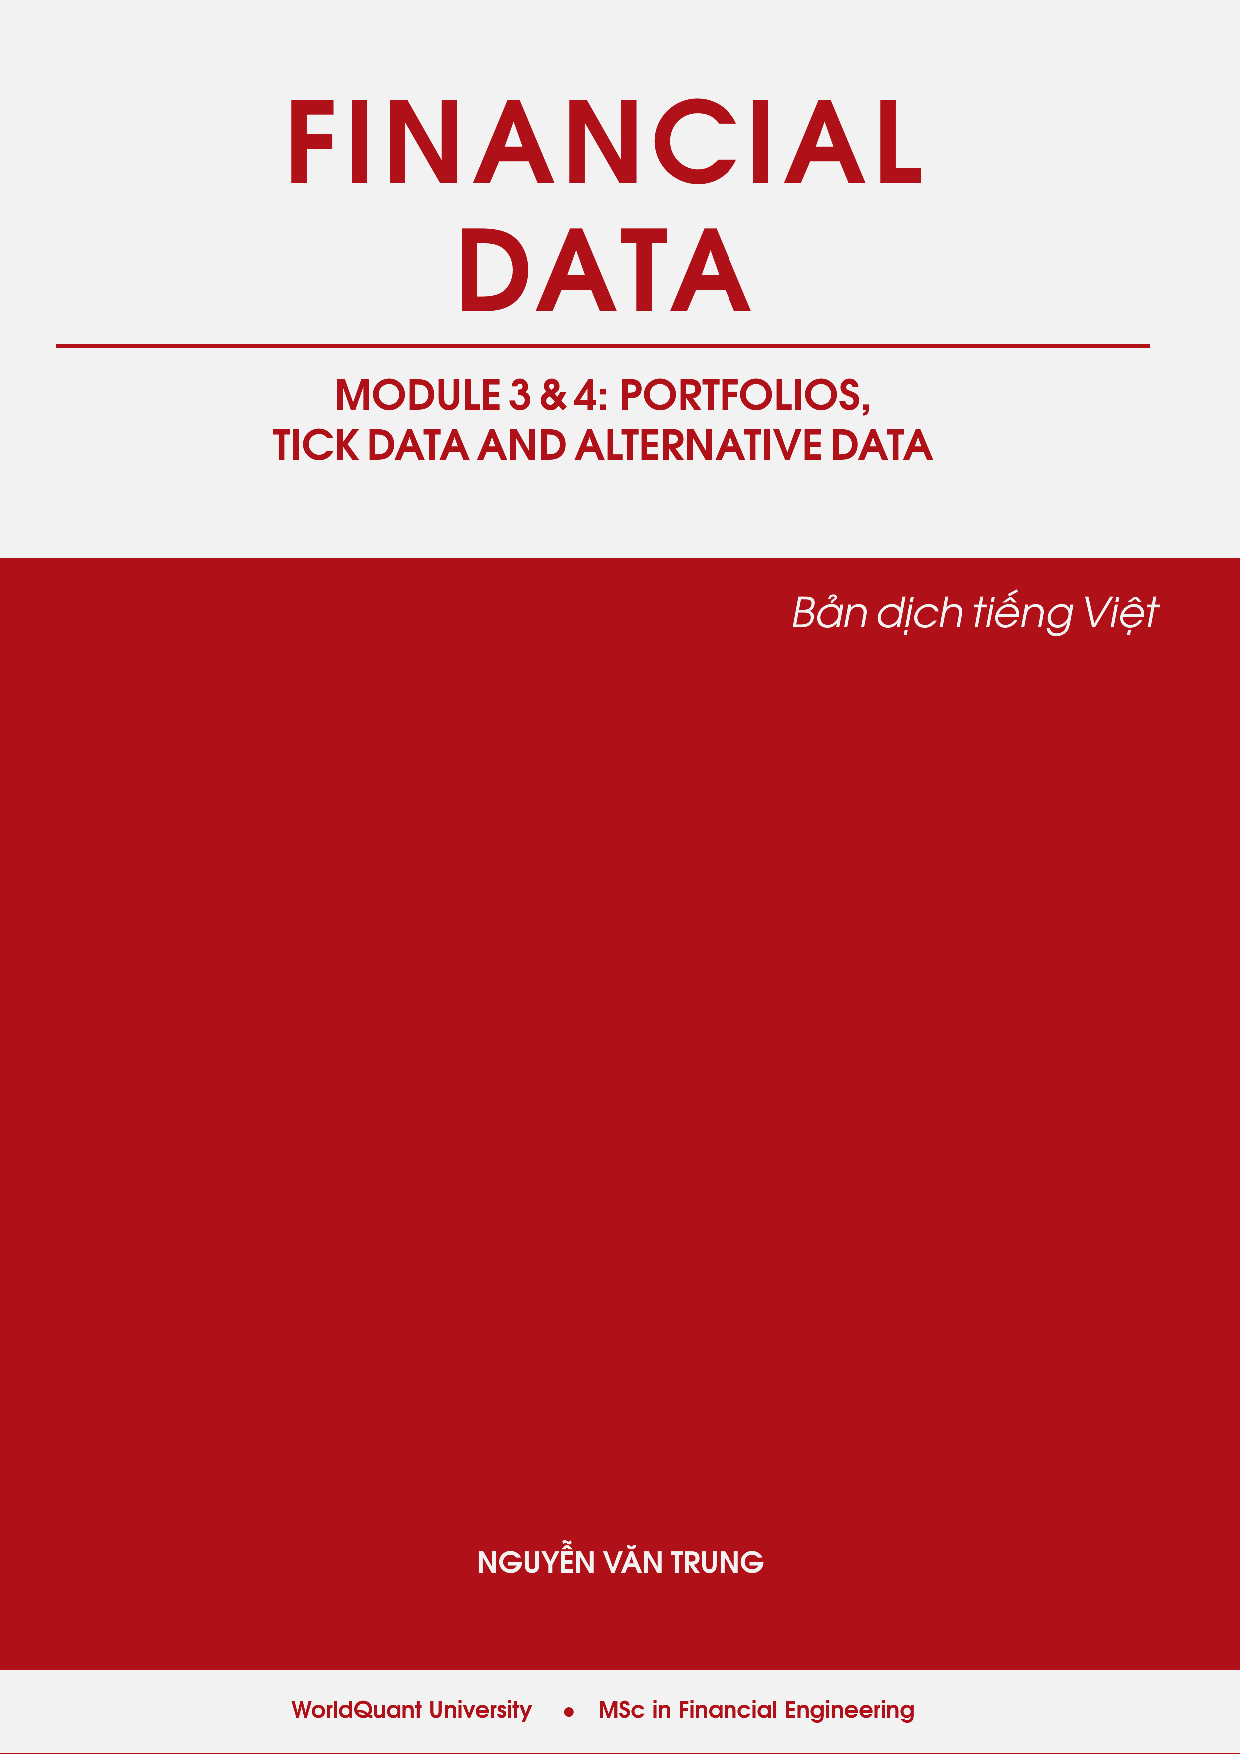
\includepdf[pages=-]{gfx/cover.pdf}}{}
%!TEX root = main-wqu-financial-data-module5-6-dich.tex
% ===================================================================
% DISCLAIMER — Nguồn tài liệu và giấy phép
% ===================================================================

\pdfbookmark[1]{\spacedallcaps{Disclaimer}}{disclaimer}

\thispagestyle{empty}

\section*{Mục đích tài liệu}

Tài liệu này là bản chuyển ngữ cá nhân, được biên soạn phục vụ \textbf{mục đích học tập và nghiên cứu cá nhân} của học viên chương trình Master of Science in Financial Engineering tại WorldQuant University, không nhằm mục đích thương mại và không được phân phối công khai.

Nội dung gồm hai phần:
\begin{itemize}
  \item \textbf{Lesson Notes} do WorldQuant University (WQU) biên soạn cho học viên của khóa học (Module 5 và Module 6).
  \item \textbf{Các bài đọc thêm (Required Readings)} là tài liệu của bên thứ ba. Chỉ phần WQU yêu cầu đọc được chuyển ngữ sang tiếng Việt dưới dạng \textbf{bản súc tích, bám cấu trúc nguồn} (giữ tiêu đề, công thức, số liệu, bảng, chú thích và tài liệu tham khảo); đây không phải bản dịch từng câu chữ.
\end{itemize}

Bản dịch là tác phẩm phái sinh: không phải bản chính thức và không được tác giả hay nhà xuất bản của các tài liệu gốc xác nhận. Khi cần trích dẫn hoặc đối chiếu, vui lòng dùng bản gốc tiếng Anh theo các đường dẫn bên dưới.

\section*{Giấy phép của từng tài liệu}

{\small
\renewcommand{\arraystretch}{1.25}
\begin{longtable}{>{\raggedright\arraybackslash}p{0.34\linewidth}>{\raggedright\arraybackslash}p{0.60\linewidth}}
\toprule
\textbf{Tài liệu} & \textbf{Giấy phép / bản quyền} \\
\midrule
\endhead
\textbf{Lesson Notes}, WorldQuant University (Module 5, Module 6). &
Bản quyền © 2024 WorldQuant University. Nội dung chỉ được cấp phép cho mục đích sử dụng cá nhân; nghiêm cấm phân phối lại hoặc xuất bản. \\
\addlinespace
Các bài đọc thêm (Required Readings) & Tài liệu của bên thứ ba (bài báo, trang web, ghi chú bài giảng); bản quyền thuộc tác giả và nhà xuất bản tương ứng. Bản chuyển ngữ chỉ phục vụ học tập cá nhân; xem nguồn gốc ở đầu mỗi chương \textit{Đọc thêm}. \\
\addlinespace
\bottomrule
\end{longtable}
}

\section*{Ghi chú}

Hình ảnh và biểu đồ trong các bài đọc thêm được trích trực tiếp từ tài liệu gốc, thuộc cùng phạm vi giấy phép của từng tài liệu; hình trong Lesson Notes là kết quả chạy mã của chính bài học.


\pagestyle{scrheadings}
\tableofcontents
\cleardoublepage
\pagenumbering{arabic}

% ============ MODULE 5 ============
% ---- Lesson 1 ----
\chapter{Phân rã ma trận không âm (Non-Negative Matrix Factorization)}
\label{ch:M5L1LessonNotes}

\section*{Lesson Notes}

MODULE 5 \textbar{} BÀI 1

\begin{center}\rule{0.5\linewidth}{0.5pt}\end{center}

{\small
\begin{longtable}[]{@{}
  >{\raggedright\arraybackslash}p{(\columnwidth - 2\tabcolsep) * \real{0.2182}}
  >{\raggedright\arraybackslash}p{(\columnwidth - 2\tabcolsep) * \real{0.7697}}@{}}
\toprule\noalign{}
\endhead
\bottomrule\noalign{}
\endlastfoot
\textbf{Thời gian đọc} & 50 phút \\
\textbf{Kiến thức nền tảng} & \begin{minipage}[t]{\linewidth}\raggedright
Hiểu biết cơ bản về đại số tuyến tính và thống kê: ma trận và vectơ; giá trị riêng và vectơ riêng; thống kê cơ bản;\\
Quen thuộc với lập trình Python: cú pháp Python cơ bản, xử lý dữ liệu và các phép toán số học;\\
Các khái niệm tài chính cơ bản: lợi suất tài sản và tương quan; đa dạng hóa danh mục đầu tư; phân tích cảm xúc\strut
\end{minipage} \\
\textbf{Từ khóa} & \begin{minipage}[t]{\linewidth}\raggedright
Phân rã ma trận không âm (NMF), giảm chiều dữ liệu, trích xuất đặc trưng, biểu diễn theo thành phần (parts-based representation),\\
tính thưa (sparsity), khả năng diễn giải, NMF thưa (Sparse NMF), NMF có ràng buộc (Constrained NMF), Semi-NMF, Convex NMF, NMF trực tuyến (Online NMF), phân tích cảm xúc,\\
Phân tích thành phần chính (PCA), Phân rã giá trị suy biến (SVD), Phân tích thành phần độc lập (ICA),\\
hệ số tải nhân tố (factor loadings), điểm số nhân tố (factor scores)\strut
\end{minipage} \\
\end{longtable}
}

\begin{center}\rule{0.5\linewidth}{0.5pt}\end{center}

\emph{Trong bài học này, chúng ta tìm hiểu phân rã ma trận không âm (NMF), một kỹ thuật phân rã một ma trận không âm thành hai ma trận không âm nhỏ hơn. Kỹ thuật này thường được dùng để giảm chiều dữ liệu, trích xuất đặc trưng và mô hình hóa chủ đề. Bài học cung cấp cái nhìn tổng quan toàn diện về NMF, các biến thể và ứng dụng của nó, với trọng tâm là kỹ thuật tài chính, đặc biệt là đa dạng hóa danh mục đầu tư.}

In {[}1{]}:

\begin{lstlisting}[escapeinside={(*@}{@*)}]
# Loading libraries
import pandas as pd
import yfinance as yf

from sklearn.decomposition import NMF
\end{lstlisting}

\section{Phân rã ma trận không âm là gì?}

Phân rã ma trận không âm (non-negative matrix factorization, NMF) là một kỹ thuật giảm chiều dữ liệu, trong đó một ma trận không âm được phân rã thành hai ma trận không âm nhỏ hơn. Kỹ thuật này thường được dùng trong phân tích dữ liệu, học máy và các hệ thống gợi ý. Hãy xem lại các tài liệu đọc bắt buộc rồi quay lại với phần còn lại của bài học này.

Định nghĩa toán học của phân rã ma trận không âm (NMF) như sau:

Cho một ma trận không âm \(V\) có kích thước \(m \times n\), NMF tìm hai ma trận không âm:

\begin{itemize}
\item
  \(W\) có kích thước \(m \times k\) (\(m\) hàng, \(k\) cột, trong đó \(k\) là số chiều sau khi giảm);
\item
  \(H\) có kích thước \(k \times n\);
\end{itemize}

sao cho: \[
V \approx W * H
\]

Trong đó:

\begin{itemize}
\item
  \(*\) ký hiệu phép nhân ma trận
\item
  Phép xấp xỉ \(\approx\) thường được đo bằng một hàm chi phí, chẳng hạn chuẩn Frobenius: \(\lVert V - W * H \rVert ^2\)
\end{itemize}

Ràng buộc: Mọi phần tử của \(W\) và \(H\) phải là số thực không âm, tức là \(W\) \ensuremath{\geq} 0, \(H\) \ensuremath{\geq} 0

Nói đơn giản, ta muốn tìm hai ma trận (\(W\) và \(H\)) sao cho khi nhân với nhau, kết quả xấp xỉ sát ma trận dữ liệu gốc (\(V\)). Các phần tử của \(W\) và \(H\) phải không âm (lớn hơn hoặc bằng không).

Hạng phân rã (factorization rank) trong NMF, thường ký hiệu là \(k\), biểu thị số lượng nhân tố hay thành phần mà ta muốn trích xuất từ dữ liệu. Về bản chất, nó quyết định số chiều của biểu diễn đã giảm chiều.

\textbf{Quy tắc cập nhật lặp:} Có nhiều cách để tìm \(W\) và \(H\). Các thuật toán NMF thường dùng quy tắc cập nhật lặp để tinh chỉnh các ma trận \(W\) và \(H\) cho đến khi hội tụ. Các quy tắc này nhằm cực tiểu hóa sự khác biệt giữa ma trận gốc \(V\) và tích \(W * H\). Một quy tắc cập nhật phổ biến là quy tắc cập nhật nhân (multiplicative update rule), được suy ra từ việc cực tiểu hóa chuẩn Frobenius:

\[
W_{ia} \leftarrow W_{ia} * \frac{(V * H^T)_{ia}}{(W * H * H^T)_{ia}}
\]

\[
H_{aj} \leftarrow H_{aj} * \frac{(W^T * V)_{aj}}{(W^T * W * H)_{aj}}
\]

Trong đó:

\begin{itemize}
\item
  \(W_{ia}\) biểu diễn phần tử ở hàng thứ \(i\) và cột thứ \(a\) của ma trận \(W\).
\item
  \(H_{aj}\) biểu diễn phần tử ở hàng thứ \(a\) và cột thứ \(j\) của ma trận \(H\).
\item
  \(V\), \(W\) và \(H\) là các ma trận như đã định nghĩa trong bài toán NMF.
\item
  \(H^T\) và \(W^T\) lần lượt là ma trận chuyển vị của \(H\) và \(W\).
\item
  \(*\) và phép chia lần lượt biểu thị phép nhân và phép chia theo từng phần tử.
\end{itemize}

Quá trình lặp tiếp tục cho đến khi thỏa mãn một tiêu chí hội tụ. Tiêu chí này có thể dựa trên:

\begin{itemize}
\item
  Sự chênh lệch của hàm chi phí: Thuật toán dừng khi mức thay đổi của hàm chi phí (ví dụ chuẩn Frobenius) giữa hai lần lặp liên tiếp nhỏ hơn một ngưỡng định trước.
\item
  Số lần lặp tối đa: Thuật toán kết thúc sau một số lần lặp cố định, ngay cả khi hàm chi phí chưa hội tụ hoàn toàn.
\end{itemize}

Về mặt toán học, sự hội tụ có thể được biểu diễn như sau:

\[
\lVert V - W^{(t+1)} * H^{(t+1)} \rVert ^2 - \lVert V - W^{(t)} * H^{(t)} \rVert ^2 < \varepsilon
\]

Trong đó:

\begin{itemize}
\item
  \(W^{(t)}\) và \(H^{(t)}\) biểu diễn các ma trận \(W\) và \(H\) tại lần lặp \(t\).
\item
  \(\varepsilon\) là một giá trị dương nhỏ biểu thị ngưỡng hội tụ.
\end{itemize}

Nói đơn giản, thuật toán dừng khi sai khác về sai số xấp xỉ giữa hai lần lặp liên tiếp trở nên đủ nhỏ.

\section{Ứng dụng của phân rã ma trận không âm (NMF) trong kỹ thuật tài chính}

NMF ngày càng phổ biến trong kỹ thuật tài chính nhờ khả năng trích xuất các đặc trưng có ý nghĩa và dễ diễn giải từ dữ liệu tài chính. Dưới đây là một số ứng dụng đáng chú ý:

\textbf{Đa dạng hóa danh mục đầu tư:} NMF có thể được dùng để xác định các nhóm tài sản có hành vi tương tự nhau, từ đó xây dựng các danh mục đầu tư đa dạng hóa với rủi ro thấp hơn. Bằng cách phân rã ma trận tương quan của lợi suất tài sản, NMF có thể làm lộ ra các nhân tố tiềm ẩn chi phối sự đồng biến động của các tài sản và giúp nhà đầu tư phân bổ vốn giữa các nhóm tài sản khác nhau.

\textbf{Quản trị rủi ro:} NMF có thể được dùng để nhận diện và định lượng các nhân tố rủi ro trên thị trường tài chính. Bằng cách phân rã dữ liệu thị trường lịch sử, NMF có thể phát hiện các nhân tố rủi ro ẩn mà các phương pháp truyền thống có thể không nhận ra. Thông tin này có thể được dùng để xây dựng các chiến lược quản trị rủi ro và cải thiện việc phòng ngừa rủi ro cho danh mục đầu tư.

\textbf{Định giá tài sản:} NMF có thể được áp dụng vào các mô hình định giá tài sản để xác định các nhân tố giải thích lợi suất tài sản. Bằng cách phân rã mặt cắt ngang của lợi suất tài sản, NMF có thể làm lộ ra các nhân tố tiềm ẩn chi phối giá tài sản và giúp nhà đầu tư hiểu các yếu tố quyết định hiệu quả của tài sản.

\textbf{Phân tích cảm xúc:} NMF có thể được dùng để phân tích dữ liệu văn bản, chẳng hạn các bài báo hoặc bài đăng trên mạng xã hội, nhằm trích xuất cảm xúc và đánh giá cảm xúc thị trường đối với các tài sản cụ thể hoặc toàn bộ thị trường. Thông tin này có thể được dùng để hỗ trợ các quyết định đầu tư và dự đoán biến động thị trường.

\textbf{Phát hiện gian lận:} NMF có thể được dùng để phát hiện các bất thường và mẫu hình trong các giao dịch tài chính có thể là dấu hiệu của hoạt động gian lận. Bằng cách phân rã dữ liệu giao dịch, NMF có thể nhận diện các mẫu hình bất thường và làm nổi bật những khu vực đáng lưu ý cần điều tra thêm.

\textbf{Giao dịch tần suất cao:} NMF có thể được dùng để phân tích dữ liệu tài chính tần suất cao và xác định các mẫu hình có thể khai thác cho các chiến lược giao dịch. Bằng cách phân rã dữ liệu giá và khối lượng, NMF có thể làm lộ ra các mối quan hệ ẩn và dự đoán biến động giá ngắn hạn.

\textbf{Giao dịch thuật toán:} NMF có thể được tích hợp vào các hệ thống giao dịch thuật toán để tự động hóa các quyết định giao dịch dựa trên các đặc trưng và mẫu hình được trích xuất từ dữ liệu tài chính. Điều này có thể giúp nâng cao hiệu quả và khả năng sinh lời của hoạt động giao dịch.

Đây chỉ là một vài ví dụ về cách NMF đang được áp dụng trong kỹ thuật tài chính. Khả năng trích xuất các đặc trưng có ý nghĩa và dễ diễn giải từ dữ liệu tài chính phức tạp khiến NMF trở thành công cụ có giá trị cho nhiều tác vụ, bao gồm quản lý danh mục đầu tư, quản trị rủi ro, định giá tài sản và giao dịch. Khi thị trường tài chính ngày càng phức tạp và dựa nhiều vào dữ liệu, các ứng dụng của NMF trong kỹ thuật tài chính nhiều khả năng sẽ tiếp tục mở rộng.

\section{Ví dụ minh họa đơn giản}

Hãy minh họa cách thủ tục NMF vận hành bằng một ví dụ đơn giản nhỏ này. Xét ma trận dữ liệu \(V\) kích thước 4x5 như sau:

\[V = \begin{pmatrix} 1 & 2 & 3 & 4 & 5 \\ 6 & 7 & 8 & 9 & 10 \\ 11 & 12 & 13 & 14 & 15 \\ 16 & 17 & 18 & 19 & 20 \\ \end{pmatrix}\]

Chúng ta muốn phân rã ma trận này thành hai ma trận nhỏ hơn, \(W\) (4x2) và \(H\) (2x5), sao cho \(V \ensuremath{\approx} W * H\). Chúng ta khởi tạo \(W^{(0)}\) (ma trận đặc trưng tại \(t=0\)) và \(H^{(0)}\) (ma trận hệ số tại \(t=0\)) bằng các giá trị không âm ngẫu nhiên:

\[W^{(0)} = \begin{pmatrix} 0.2 & 0.5 \\ 0.8 & 0.3 \\ 0.6 & 0.9 \\ 0.4 & 0.7 \\ \end{pmatrix}, \quad H^{(0)} = \begin{pmatrix} 0.7 & 0.1 & 0.4 & 0.6 & 0.2 \\ 0.3 & 0.6 & 0.2 & 0.4 & 0.8 \\ \end{pmatrix}\]

Bây giờ, chúng ta cập nhật lặp \(W^{(t)}\) và \(H^{(t)}\) bằng các quy tắc cập nhật nhân để cực tiểu hóa sự chênh lệch giữa \(V\) và \(W^{(t)} * H^{(t)}\). Sau một vài vòng lặp, chúng ta có thể thu được các ma trận đã cập nhật như sau:

\[W = \begin{pmatrix} 0.9618 & 0. \\ 1.9262 & 1.0167 \\ 2.8902 & 2.0347 \\ 3.8542 & 3.0527 \\ \end{pmatrix}, \quad H = \begin{pmatrix} 1.0413 & 2.0823 & 3.1232 & 4.1642 & 5.19 \\ 3.9269 & 2.9399 & 1.9529 & 0.966 & 0. \\ \end{pmatrix}\]

Giá trị cuối cùng của ma trận đặc trưng \(W\) và ma trận hệ số \(H\) biểu diễn các nhân tử phân rã của ma trận gốc \(V\). Lưu ý rằng các giá trị cụ thể trong các ma trận có thể khác đôi chút tùy thuộc vào phép tính thực tế. Bằng cách nhân \(W\) và \(H\), chúng ta thu được một xấp xỉ của \(V\):

\[W * H = \begin{pmatrix} 1.0015 & 2.0028 & 3.004 & 4.0052 & 4.9919 \\ 5.9983 & 6.9999 & 8.0017 & 9.0034 & 9.9972 \\ 10.9996 & 12. & 13.0004 & 14.0008 & 15.0002 \\ 16.0009 & 17. & 17.9992 & 18.9983 & 20.0032 \\ \end{pmatrix}\]

Ma trận kết quả này là một xấp xỉ của ma trận gốc \(V\). Sự chênh lệch giữa \(V\) và \(W * H\) biểu diễn sai số tái tạo.

\[V - W * H = \begin{pmatrix} -0.0015 & -0.0028 & -0.004 & -0.0052 & 0.0081 \\ 0.0017 & 0.0001 & -0.0017 & -0.0034 & 0.0028 \\ 0.0004 & 0. & -0.0004 & -0.0008 & -0.0002 \\ -0.0009 & -0. & 0.0008 & 0.0017 & -0.0032 \\ \end{pmatrix}\]

Mục tiêu của NMF là tìm \(W\) và \(H\) sao cho cực tiểu hóa sai số tái tạo này, đồng thời giữ cho mọi phần tử của \(W\) và \(H\) đều không âm.

Ví dụ số rất đơn giản này cho thấy NMF có thể phân rã một ma trận dữ liệu lớn hơn thành các ma trận nhỏ hơn, nắm bắt cấu trúc tiềm ẩn và các mối quan hệ của nó.

\section{Cơ bản về phân rã ma trận không âm (NMF)}

Nói ngắn gọn, NMF là việc tìm một cách biểu diễn đơn giản hơn của dữ liệu bằng cách tách nó thành hai phần nắm bắt các đặc trưng thiết yếu và mức độ quan trọng của chúng. NMF có ứng dụng trong nhiều lĩnh vực, bao gồm xử lý ảnh, phân tích văn bản và tin sinh học. Việc triển khai bao gồm các bước sau:

\begin{itemize}
\item
  \textbf{Khởi tạo:} Bắt đầu với một ma trận không âm, thường được ký hiệu là \(V\), biểu diễn dữ liệu. Đây là ma trận chứa thông tin về người dùng, sản phẩm hoặc bất kỳ loại dữ liệu nào khác.
\item
  \textbf{Phân rã:} Cốt lõi của NMF là tìm hai ma trận không âm, thường được gọi là \(W\) và \(H\), sao cho tích của \(W\) và \(H\) xấp xỉ sát ma trận gốc \(V\), tức là \(V \approx WH\). Nói đơn giản hơn, chúng ta đang cố gắng tách dữ liệu gốc thành hai phần mà khi kết hợp lại sẽ giống với dữ liệu ban đầu.
\item
  \textbf{Lặp:} Các thuật toán NMF sử dụng các quy trình lặp để tinh chỉnh \(W\) và \(H\), nhằm cực tiểu hóa sự chênh lệch giữa tích \(W H\) và ma trận gốc \(V\). Các vòng lặp này cập nhật \(W\) và \(H\) nhiều lần cho đến khi đạt được mức độ chính xác thỏa đáng. Quy trình này thường dựa trên hạ gradient (gradient descent) hoặc các phép cập nhật nhân tính.
\item
  \textbf{Hội tụ:} Quá trình lặp tiếp tục cho đến khi thỏa mãn một tiêu chí hội tụ. Điều này thường có nghĩa là sự chênh lệch giữa \(W H\) và \(V\) đã đủ nhỏ, hoặc thuật toán đã chạy đủ một số bước định trước.
\item
  \textbf{Diễn giải:} Sau khi hội tụ, các ma trận \(W\) và \(H\) thu được cung cấp một biểu diễn có chiều thấp hơn của dữ liệu gốc. Có thể xem \(W\) chứa các vectơ cơ sở hay các đặc trưng, còn \(H\) biểu diễn các hệ số hay trọng số của những đặc trưng này đối với từng điểm dữ liệu. Mỗi cột của \(W\) biểu diễn một đặc trưng, và hàng tương ứng của \(H\) cho biết đặc trưng này được thể hiện mạnh đến mức nào trong từng điểm dữ liệu.
\end{itemize}

\section{Các tính chất của phân rã ma trận không âm (NMF)}

Một số tính chất quan trọng của phân rã ma trận không âm (non-negative matrix factorization, NMF) là:

\textbf{Tính không âm:} Tính chất cơ bản nhất của NMF là nó tạo ra các ma trận không âm \(W\) và \(H\). Điều này có nghĩa là mọi phần tử của các ma trận này đều lớn hơn hoặc bằng không. Tính chất này rất quan trọng đối với khả năng diễn giải, vì nó cho phép ta hiểu các nhân tố thu được như những tổ hợp cộng tính của các đặc trưng ban đầu.

\textbf{Giảm chiều dữ liệu:} NMF giảm số chiều của dữ liệu bằng cách phân rã nó thành hai ma trận có hạng thấp hơn. Điều này hữu ích để đơn giản hóa dữ liệu, loại bỏ nhiễu và xác định các đặc trưng tiềm ẩn.

\textbf{Biểu diễn theo bộ phận:} NMF thường dẫn đến một biểu diễn dữ liệu theo bộ phận (parts-based representation). Điều này có nghĩa là các nhân tố thu được (các cột của \(W\)) có thể được diễn giải là đại diện cho từng bộ phận hoặc thành phần riêng lẻ của dữ liệu gốc. Chẳng hạn, trong phân tích ảnh, NMF có thể xác định các nhân tố tương ứng với cạnh, kết cấu hoặc đối tượng.

\textbf{Tính thưa:} NMF thường tạo ra các ma trận thưa, nghĩa là nhiều phần tử của \(W\) và \(H\) bằng không. Điều này có lợi cho khả năng diễn giải, vì nó làm nổi bật các đặc trưng quan trọng nhất và giảm độ phức tạp của mô hình.

\textbf{Khả năng diễn giải:} Nhờ tính không âm và biểu diễn theo bộ phận, NMF thường được coi là dễ diễn giải hơn các kỹ thuật giảm chiều dữ liệu khác như Phân tích thành phần chính (Principal Component Analysis, PCA). Các nhân tố thu được có thể được liên hệ dễ dàng hơn với các đặc trưng ban đầu, giúp việc hiểu cấu trúc tiềm ẩn của dữ liệu trở nên dễ dàng hơn.

\textbf{Tính linh hoạt:} NMF có thể được áp dụng cho nhiều loại dữ liệu khác nhau, bao gồm văn bản, hình ảnh, âm thanh và dữ liệu sinh học. Nó cũng có thể được điều chỉnh cho các ứng dụng khác nhau bằng cách sử dụng các hàm chi phí và ràng buộc khác nhau.

\textbf{Hiệu quả tính toán:} Các thuật toán NMF nhìn chung có hiệu quả về mặt tính toán, đặc biệt đối với dữ liệu thưa. Điều này khiến chúng phù hợp với các tập dữ liệu quy mô lớn.

\textbf{Tính không duy nhất:} Phép phân rã NMF không duy nhất, nghĩa là có thể tồn tại nhiều nghiệm cho \(W\) và \(H\) cùng xấp xỉ tốt \(V\). Vấn đề này có thể được giải quyết bằng cách sử dụng các kỹ thuật chính quy hóa hoặc áp đặt thêm các ràng buộc.

Trên đây là một số tính chất quan trọng của NMF. Chúng góp phần làm nên sự phổ biến và hiệu quả của NMF trong nhiều tác vụ phân tích dữ liệu và học máy.

\section{Thách thức và hạn chế của phân rã ma trận không âm (NMF)}

Phân rã ma trận không âm (NMF) có một số thách thức và hạn chế:

\textbf{Tính không duy nhất của nghiệm:} Phép phân rã NMF vốn không duy nhất, nghĩa là có thể tồn tại nhiều cặp ma trận nhân tử (\(W\) và \(H\)) mà khi nhân với nhau đều xấp xỉ ma trận dữ liệu gốc (\(V\)) tốt như nhau. Điều này xuất phát từ việc thường có nhiều cách biểu diễn cùng một dữ liệu bằng các tổ hợp nhân tử không âm khác nhau.

\begin{quote}
\begin{itemize}
\item
  Hệ quả: Tính không duy nhất này gây khó khăn cho việc diễn giải kết quả của NMF, vì các nghiệm khác nhau có thể dẫn đến những cách diễn giải khác nhau về các nhân tử tiềm ẩn. Nó cũng khiến việc so sánh kết quả giữa các lần chạy khác nhau của thuật toán, hoặc khi dùng các chiến lược khởi tạo khác nhau, trở nên khó khăn.
\item
  Giải pháp: Các kỹ thuật như chính quy hóa (regularization), vốn bổ sung ràng buộc hoặc hình phạt vào hàm mục tiêu, có thể giúp giảm bớt vấn đề không duy nhất bằng cách khuyến khích các nghiệm có những tính chất cụ thể, chẳng hạn như tính thưa hoặc tính trực giao.
\end{itemize}
\end{quote}

\textbf{Độ nhạy với khởi tạo:} Hiệu năng của các thuật toán NMF có thể nhạy với giá trị khởi tạo của các ma trận nhân tử (\(W\) và \(H\)). Các chiến lược khởi tạo khác nhau có thể khiến thuật toán hội tụ về các cực tiểu cục bộ khác nhau, dẫn đến các nghiệm khác nhau.

\begin{quote}
\begin{itemize}
\item
  Hệ quả: Độ nhạy với khởi tạo này làm cho kết quả của NMF kém khả năng tái lập hơn và có thể dẫn đến các nghiệm dưới tối ưu.
\item
  Giải pháp: Thử nhiều phương pháp khởi tạo khác nhau, chẳng hạn khởi tạo ngẫu nhiên, NNDSVD (phân rã giá trị suy biến kép không âm - Non-negative Double Singular Value Decomposition), hoặc tận dụng kiến thức có sẵn về dữ liệu, có thể giúp giảm nhẹ vấn đề này và có khả năng cải thiện chất lượng nghiệm.
\end{itemize}
\end{quote}

\textbf{Xác định số lượng nhân tử tối ưu:} Chọn đúng số lượng nhân tử (hay thành phần) là một bước then chốt trong NMF. Quá ít nhân tử có thể không nắm bắt được hết thông tin quan trọng trong dữ liệu, dẫn đến mất thông tin và giảm độ chính xác. Quá nhiều nhân tử có thể dẫn đến quá khớp (overfitting), khi đó mô hình nắm bắt nhiễu hoặc các mẫu không liên quan trong dữ liệu, làm giảm khả năng khái quát hóa sang dữ liệu mới.

\begin{quote}
\begin{itemize}
\item
  Hệ quả: Việc chọn số lượng nhân tử không phù hợp có thể ảnh hưởng đáng kể đến hiệu năng và khả năng diễn giải của mô hình NMF.
\item
  Giải pháp: Các kỹ thuật lựa chọn mô hình, chẳng hạn kiểm định chéo (cross-validation), phân tích silhouette, hoặc dùng chuyên môn lĩnh vực để đánh giá khả năng diễn giải của các nhân tử, có thể giúp định hướng việc chọn số lượng nhân tử tối ưu.
\end{itemize}
\end{quote}

\textbf{Yêu cầu dữ liệu không âm:} NMF về cơ bản được thiết kế để làm việc với dữ liệu không âm. Thuật toán giả định rằng ma trận dữ liệu đầu vào (\(V\)) và các ma trận nhân tử kết quả (\(W\) và \(H\)) chỉ có các phần tử không âm. Lý do là ràng buộc không âm đóng vai trò thiết yếu để bảo đảm các nhân tử có thể diễn giải được như những tổ hợp cộng tính của các đặc trưng ban đầu.

\begin{quote}
\begin{itemize}
\item
  Hệ quả: Hạn chế này giới hạn khả năng áp dụng NMF vào các tập dữ liệu mà giá trị âm không có ý nghĩa, hoặc có thể được chuyển thành biểu diễn không âm.
\item
  Giải pháp: Với dữ liệu có giá trị âm, có thể cân nhắc các kỹ thuật như dịch chuyển (cộng một hằng số vào mọi phần tử), co giãn (nhân với một hằng số dương), hoặc dùng các phương pháp phân rã ma trận khác có thể xử lý dữ liệu có dấu hỗn hợp.
\end{itemize}
\end{quote}

\textbf{Thách thức về khả năng diễn giải:} Mặc dù NMF thường được xem là dễ diễn giải hơn các kỹ thuật giảm chiều dữ liệu khác như PCA, việc diễn giải các nhân tử kết quả vẫn có thể mang tính chủ quan và đòi hỏi chuyên môn lĩnh vực. Các nhân tử biểu diễn những đặc trưng hoặc mẫu tiềm ẩn trong dữ liệu, và ý nghĩa của chúng không phải lúc nào cũng rõ ràng ngay lập tức.

\begin{quote}
\begin{itemize}
\item
  Hệ quả: Việc diễn giải các nhân tử NMF đòi hỏi phân tích cẩn thận và xem xét bối cảnh của dữ liệu cũng như ứng dụng cụ thể.
\item
  Giải pháp: Các kỹ thuật như trực quan hóa các hệ số tải của nhân tử (factor loadings), xem xét các đặc trưng đóng góp nhiều nhất cho từng nhân tử, và dùng kiến thức lĩnh vực để liên hệ các nhân tử với các khái niệm trong thế giới thực có thể hỗ trợ việc diễn giải.
\end{itemize}
\end{quote}

\textbf{Chi phí tính toán:} Các thuật toán NMF có thể tốn kém về mặt tính toán, đặc biệt với các tập dữ liệu lớn hoặc số lượng nhân tử cao. Bản chất lặp của thuật toán và nhu cầu cập nhật các ma trận nhân tử nhiều lần có thể dẫn đến thời gian tính toán đáng kể.

\begin{quote}
\begin{itemize}
\item
  Hệ quả: Chi phí tính toán của NMF có thể là một yếu tố hạn chế đối với các ứng dụng quy mô lớn hoặc khi cần phân tích theo thời gian thực.
\item
  Giải pháp: Sử dụng các thuật toán hiệu quả, chẳng hạn những thuật toán dựa trên các phép toán ma trận thưa, có thể giúp giảm gánh nặng tính toán. Ngoài ra, các kỹ thuật như NMF trực tuyến (online NMF), vốn cập nhật phép phân rã theo từng bước khi có dữ liệu mới đến, có thể dễ xử lý hơn về mặt tính toán đối với dữ liệu dòng (streaming).
\end{itemize}
\end{quote}

\section{So sánh NMF với các kỹ thuật phân rã ma trận khác}

\textbf{Phân tích thành phần chính (Principal component analysis -- PCA)} là một kỹ thuật giảm chiều dữ liệu, biến đổi dữ liệu nhiều chiều sang không gian có số chiều thấp hơn bằng cách xác định các hướng (thành phần chính) mà dữ liệu biến thiên nhiều nhất. Các thành phần chính này trực giao với nhau và nắm bắt phương sai tối đa của dữ liệu, cho phép đơn giản hóa dữ liệu, giảm nhiễu và trích xuất đặc trưng. PCA thường được dùng để trực quan hóa dữ liệu, giảm nhiễu và làm bước tiền xử lý cho học máy. Đây là kỹ thuật linh hoạt, áp dụng được cho nhiều loại dữ liệu, nhưng các thành phần thu được có thể khó diễn giải hơn. Tóm lại, PCA tìm ra các mẫu quan trọng nhất trong dữ liệu và biểu diễn chúng bằng một số ít biến (các thành phần chính) trực giao. Điều này giúp đơn giản hóa dữ liệu mà vẫn giữ được thông tin cốt lõi.

\textbf{Phân rã giá trị suy biến (Singular value decomposition -- SVD)} là một kỹ thuật phân rã ma trận đa dụng hơn, phân rã dữ liệu thành ba ma trận, nắm bắt các nhân tố ẩn và mối quan hệ giữa chúng. SVD là kỹ thuật phân rã ma trận thành ba ma trận thành phần: \(U\), \(\Sigma\) và \(V^T\). Các ma trận này nắm bắt các nhân tố ẩn và các mối quan hệ trong dữ liệu, cho phép giảm chiều dữ liệu, giảm nhiễu và nén dữ liệu. SVD được sử dụng rộng rãi trong nhiều ứng dụng, bao gồm hệ thống gợi ý, nén ảnh và giảm nhiễu. Tuy nhiên, giống như PCA, các thành phần của SVD có thể khó diễn giải hơn. Tóm lại, SVD tách một ma trận thành các thành phần đơn giản hơn, qua đó bộc lộ cấu trúc và các mối quan hệ tiềm ẩn của nó.

\textbf{Phân tích thành phần độc lập (Independent component analysis -- ICA)} là một kỹ thuật tính toán nhằm tách một tín hiệu đa biến thành các thành phần con cộng tính, độc lập về mặt thống kê và không tuân theo phân phối Gauss. Tóm lại, ICA nhằm khám phá các nguồn hoặc nhân tố ẩn đóng góp vào một tín hiệu hỗn hợp. Điều này giống như việc "tách" một ly cocktail để nhận ra từng nguyên liệu riêng lẻ.

\textbf{Phân rã ma trận không âm (Non-negative matrix factorization -- NMF)} chuyên phân rã dữ liệu không âm thành hai ma trận không âm, cho ra một biểu diễn theo bộ phận (parts-based). NMF phân rã dữ liệu không âm thành hai ma trận không âm, \(W\) và \(H\). Phép phân rã này cho ra biểu diễn theo bộ phận, trong đó các thành phần (các cột của \(W\)) đại diện cho từng bộ phận hay đặc trưng riêng của dữ liệu gốc, còn trọng số của chúng (các hàng của \(H\)) cho biết mức độ quan trọng của chúng trong từng điểm dữ liệu. Nhờ vậy, NMF đặc biệt hữu ích cho những tác vụ cần khả năng diễn giải và phân rã theo bộ phận, chẳng hạn xử lý ảnh, phân tích văn bản và mô hình hóa chủ đề. NMF thường cho kết quả thưa, làm tăng thêm khả năng diễn giải. Về bản chất, NMF tách dữ liệu thành các thành phần cộng tính, không âm, đại diện cho các bộ phận hay đặc trưng thiết yếu của dữ liệu.

PCA, SVD, ICA và NMF đều là các kỹ thuật dùng để giảm chiều dữ liệu và trích xuất đặc trưng, nhưng khác nhau về cách tiếp cận và tính chất. Những khác biệt chính là:

\begin{itemize}
\item
  \textbf{Ràng buộc:} PCA và SVD áp đặt tính trực giao lên các thành phần, ICA áp đặt tính độc lập, còn NMF áp đặt tính không âm.
\item
  \textbf{Diễn giải:} Các thành phần của PCA và SVD có thể khó diễn giải, trong khi các thành phần của ICA đại diện cho các nguồn ẩn và các thành phần của NMF thường dễ liên hệ với các đặc trưng gốc hơn.
\item
  \textbf{Tính thưa:} PCA và SVD thường cho kết quả dày đặc, trong khi ICA có thể thưa hoặc dày đặc và NMF thường dẫn đến các biểu diễn thưa.
\item
  \textbf{Kiểu dữ liệu:} PCA, SVD và ICA có thể áp dụng cho mọi kiểu dữ liệu, trong khi NMF chỉ giới hạn ở dữ liệu không âm.
\end{itemize}

Việc lựa chọn giữa PCA, SVD, ICA và NMF phụ thuộc vào ứng dụng cụ thể và các tính chất mong muốn. Nếu mục tiêu chính là nắm bắt phương sai tối đa, PCA có thể phù hợp hơn. Nếu cần một phép phân rã đa dụng hơn, SVD có thể thích hợp hơn. Nếu cần tách nguồn mù (blind source separation), ICA sẽ là kỹ thuật được ưu tiên. Nếu khả năng diễn giải và biểu diễn theo bộ phận là then chốt, NMF là lựa chọn tốt.

Trong một số trường hợp, việc kết hợp các kỹ thuật này có thể mang lại lợi ích. Ví dụ, có thể dùng PCA hoặc SVD để giảm chiều dữ liệu ban đầu, sau đó áp dụng ICA hoặc NMF để trích xuất các đặc trưng dễ diễn giải từ dữ liệu đã được giảm chiều.

\section{Các phần mở rộng của phân rã ma trận không âm (NMF)}

Mặc dù thuật toán NMF chuẩn được sử dụng rộng rãi, nhiều phần mở rộng và biến thể đã được phát triển để đáp ứng các nhu cầu cụ thể và cải thiện hiệu suất. Dưới đây là một vài biến thể đáng chú ý:

\subsection{NMF thưa (Sparse NMF)}

Phân rã ma trận không âm (NMF) thưa là một biến thể của thuật toán NMF chuẩn, trong đó áp đặt tính thưa lên các ma trận nhân tử \(W\) và \(H\). Điều này có nghĩa là thuật toán khuyến khích nhiều phần tử của các ma trận này bằng không.

\textbf{Lý do:} Tính thưa thường được mong muốn trong NMF vì một số lý do sau:

\begin{itemize}
\item
  Khả năng diễn giải: Các ma trận nhân tử thưa dễ diễn giải hơn vì chúng làm nổi bật các đặc trưng quan trọng nhất và giảm độ phức tạp của mô hình.
\item
  Lựa chọn đặc trưng: Tính thưa có thể đóng vai trò như một hình thức lựa chọn đặc trưng, xác định các đặc trưng phù hợp nhất để biểu diễn dữ liệu.
\item
  Giảm nhiễu: Bằng cách tập trung vào một tập đặc trưng nhỏ hơn, NMF thưa có thể giúp giảm ảnh hưởng của nhiễu trong dữ liệu.
\end{itemize}

\textbf{Phương pháp:} Tính thưa trong NMF thường đạt được bằng cách thêm các số hạng điều chuẩn (regularization) kích thích tính thưa vào hàm mục tiêu của NMF. Các số hạng này phạt các phần tử khác không trong các ma trận nhân tử, khuyến khích chúng tiến về không. Các kỹ thuật điều chuẩn phổ biến gồm:

\begin{itemize}
\item
  Điều chuẩn L1: Thêm một khoản phạt tỷ lệ với tổng giá trị tuyệt đối của các phần tử trong các ma trận nhân tử.
\item
  Điều chuẩn L2: Thêm một khoản phạt tỷ lệ với tổng bình phương giá trị của các phần tử trong các ma trận nhân tử.
\item
  Các ràng buộc thưa khác: Có thể dùng nhiều ràng buộc khác để thực thi tính thưa, chẳng hạn giới hạn số phần tử khác không trong mỗi hàng hoặc cột của các ma trận nhân tử.
\end{itemize}

\textbf{Lợi ích:} NMF thưa mang lại nhiều lợi ích so với NMF chuẩn:

\begin{itemize}
\item
  Cải thiện khả năng diễn giải: Các ma trận nhân tử thưa dễ hiểu hơn và dễ liên hệ với các đặc trưng gốc.
\item
  Lựa chọn đặc trưng tốt hơn: Tính thưa giúp xác định các đặc trưng phù hợp nhất để biểu diễn dữ liệu.
\item
  Giảm nhiễu: Bằng cách tập trung vào một tập đặc trưng nhỏ hơn, NMF thưa có thể giúp giảm ảnh hưởng của nhiễu.
\item
  Tăng khả năng khái quát hóa: Các mô hình thưa thường khái quát hóa tốt hơn trên dữ liệu mới vì ít bị quá khớp hơn.
\end{itemize}

\subsection{NMF có ràng buộc (Constrained NMF)}

Phân rã ma trận không âm (NMF) có ràng buộc là một biến thể của NMF chuẩn, trong đó các ràng buộc bổ sung được áp đặt lên các ma trận nhân tử (\(W\) và \(H\)) trong quá trình phân rã. Các ràng buộc này thường dựa trên kiến thức có sẵn về dữ liệu hoặc những tính chất cụ thể mong muốn ở các nhân tử thu được.

\textbf{Lý do:} Việc đưa các ràng buộc vào cho phép điều chỉnh NMF phù hợp với từng ứng dụng và đặc điểm dữ liệu. Điều này có thể cải thiện chất lượng của phép phân rã, tăng khả năng diễn giải và bảo đảm kết quả có ý nghĩa hơn trong bối cảnh của bài toán.

\textbf{Ví dụ về các ràng buộc:}

\begin{itemize}
\item
  Ràng buộc tổng bằng một: Ràng buộc này buộc các phần tử trong mỗi hàng của \(H\) (hoặc mỗi cột của \(W\)) có tổng bằng một. Ràng buộc này thường được dùng trong mô hình hóa chủ đề, khi mỗi hàng của \(H\) biểu diễn một tài liệu và các phần tử cho biết tỷ trọng của từng chủ đề trong tài liệu đó.
\item
  Ràng buộc trực giao: Ràng buộc này yêu cầu các cột của \(W\) (hoặc các hàng của \(H\)) trực giao với nhau. Nó khuyến khích các nhân tử độc lập và biểu diễn những khía cạnh khác nhau của dữ liệu.
\item
  Ràng buộc thưa: Tương tự NMF thưa, ràng buộc này thúc đẩy tính thưa trong các ma trận nhân tử, dẫn đến kết quả dễ diễn giải hơn và chống nhiễu tốt hơn.
\item
  Ràng buộc đặc thù theo lĩnh vực: Các ràng buộc dựa trên kiến thức chuyên môn có thể được đưa vào để định hướng phép phân rã. Ví dụ, trong xử lý ảnh, có thể dùng ràng buộc để bảo đảm các nhân tử biểu diễn những đặc trưng ảnh cụ thể như cạnh hoặc kết cấu bề mặt.
\end{itemize}

\textbf{Lợi ích:} NMF có ràng buộc mang lại một số ưu điểm:

\begin{itemize}
\item
  Phân rã được cải thiện: Các ràng buộc có thể định hướng quá trình phân rã tới những lời giải có ý nghĩa và phù hợp hơn.
\item
  Khả năng diễn giải được nâng cao: Các ràng buộc giúp các nhân tử thu được dễ diễn giải hơn và dễ liên hệ với dữ liệu gốc.
\item
  Lời giải được điều chỉnh theo nhu cầu: Các ràng buộc cho phép thích nghi NMF với từng ứng dụng và đặc điểm dữ liệu cụ thể.
\item
  Kiểm soát tính chất của nhân tử: Các ràng buộc có thể được dùng để áp đặt những tính chất mong muốn lên các nhân tử, chẳng hạn tính thưa, tính trực giao hoặc các mẫu cụ thể.
\end{itemize}

Về bản chất, NMF có ràng buộc cho phép bạn tùy biến thuật toán NMF theo nhu cầu cụ thể bằng cách đưa kiến thức có sẵn hoặc các tính chất mong muốn vào quá trình phân rã. Điều này có thể dẫn đến những kết quả sâu sắc và phù hợp hơn so với NMF chuẩn.

\subsection{Semi-NMF}

Semi-NMF, hay phân rã ma trận bán không âm (semi non-negative matrix factorization), là một biến thể của NMF trong đó ràng buộc không âm được nới lỏng đối với một trong hai ma trận nhân tử (\(W\) hoặc \(H\)). Điều này có nghĩa là một ma trận có thể chứa cả giá trị dương lẫn giá trị âm, trong khi ma trận còn lại vẫn không âm.

\textbf{Lý do:} Thuật toán NMF chuẩn yêu cầu mọi phần tử của các ma trận nhân tử đều không âm. Tuy nhiên, trong một số ứng dụng, các giá trị âm có thể mang ý nghĩa và cung cấp những hiểu biết giá trị. Chẳng hạn, trong phân tích dữ liệu tài chính, lợi suất âm là điều có thể xảy ra và cần được tính đến trong quá trình phân rã. Semi-NMF cho phép phân rã loại dữ liệu có dấu hỗn hợp như vậy, đồng thời vẫn giữ được các lợi ích của NMF về khả năng diễn giải và biểu diễn dựa trên các thành phần.

\textbf{Cách hoạt động:} Semi-NMF điều chỉnh hàm mục tiêu và các quy tắc cập nhật của NMF chuẩn để thích ứng với việc nới lỏng ràng buộc không âm. Thuật toán vẫn nhằm tìm hai ma trận (\(W\) và \(H\)) có tích xấp xỉ ma trận dữ liệu gốc (\(V\)), nhưng một trong hai ma trận giờ đây có thể có các phần tử âm.

\textbf{Lợi ích:}

\begin{itemize}
\item
  Xử lý dữ liệu có dấu hỗn hợp: Semi-NMF cho phép phân rã dữ liệu có cả giá trị dương và âm, điều này rất quan trọng đối với các ứng dụng mà giá trị âm có ý nghĩa.
\item
  Bảo toàn khả năng diễn giải: Dù cho phép giá trị âm, semi-NMF vẫn giữ được lợi ích của NMF về khả năng diễn giải và biểu diễn dựa trên các thành phần.
\item
  Tính linh hoạt: Phương pháp này linh hoạt hơn NMF chuẩn nhờ có thể đáp ứng nhiều loại dữ liệu hơn.
\end{itemize}

\textbf{Những điểm cần lưu ý:}

\begin{itemize}
\item
  Khi sử dụng semi-NMF, điều quan trọng là phải chọn ma trận nhân tử nào (\(W\) hay \(H\)) được phép có giá trị âm, dựa trên ứng dụng cụ thể và cách diễn giải các nhân tử.
\item
  Cách diễn giải các nhân tử có thể khác đôi chút so với NMF chuẩn do sự xuất hiện của các giá trị âm. Cần cân nhắc cẩn thận ý nghĩa của các giá trị âm trong bối cảnh của bài toán.
\end{itemize}

Tóm lại, semi-NMF là một mở rộng có giá trị của NMF, cho phép phân rã dữ liệu có dấu hỗn hợp mà vẫn giữ lại nhiều lợi ích của NMF chuẩn. Phương pháp này linh hoạt hơn và có thể mang lại hiểu biết sâu sắc về những dữ liệu mà giá trị âm có ý nghĩa.

\subsection{NMF lồi (Convex NMF)}

Phân rã ma trận không âm lồi (convex NMF) là một biến thể của NMF, trong đó các ràng buộc lồi được áp đặt lên phép phân rã. Điều này có nghĩa là các ma trận nhân tử (\(W\) và \(H\)) bị giới hạn nằm trong một tập lồi.

\textbf{Lập luận:} Việc đưa các ràng buộc lồi vào NMF có thể mang lại nhiều lợi ích:

\begin{itemize}
\item
  Tính duy nhất: NMF lồi có thể giúp giải quyết vấn đề không duy nhất vốn có của NMF chuẩn. Bằng cách giới hạn không gian nghiệm trong một tập lồi, phương pháp này có thể làm giảm số nghiệm khả dĩ và có khả năng dẫn đến một nghiệm duy nhất hoặc ổn định hơn.
\item
  Cải thiện hội tụ: Các ràng buộc lồi có thể cải thiện tính chất hội tụ của thuật toán NMF, giúp thuật toán nhiều khả năng tìm được nghiệm tốt một cách hiệu quả.
\item
  Khả năng diễn giải tốt hơn: Trong một số trường hợp, các ràng buộc lồi có thể dẫn đến các nhân tử dễ diễn giải hơn nhờ khuyến khích chúng biểu diễn những đặc trưng hoặc mẫu hình cụ thể trong dữ liệu.
\end{itemize}

\textbf{Phương pháp:} Các ràng buộc lồi trong NMF thường được áp đặt bằng cách giới hạn các ma trận nhân tử nằm trong một tập lồi. Điều này có thể thực hiện thông qua nhiều phương pháp khác nhau, chẳng hạn:

\begin{itemize}
\item
  Bao lồi (Convex Hull): Các ma trận nhân tử bị ràng buộc nằm trong bao lồi của một tập các điểm dữ liệu hoặc đặc trưng.
\item
  Ràng buộc đa diện (Polytope Constraints): Các ma trận nhân tử bị giới hạn nằm trong một đa diện cụ thể được xác định bởi một tập các bất đẳng thức tuyến tính.
\item
  Các ràng buộc lồi khác: Có thể sử dụng nhiều ràng buộc lồi khác, chẳng hạn giới hạn các ma trận nhân tử là nửa xác định dương hoặc có các cấu trúc thưa cụ thể.
\end{itemize}

\textbf{Lợi ích:} NMF lồi mang lại nhiều ưu điểm so với NMF chuẩn:

\begin{itemize}
\item
  Khả năng đạt tính duy nhất: Phương pháp này có thể giúp giải quyết vấn đề không duy nhất của NMF chuẩn, dẫn đến các nghiệm ổn định và đáng tin cậy hơn.
\item
  Cải thiện hội tụ: Các ràng buộc lồi có thể cải thiện tính chất hội tụ của thuật toán NMF.
\item
  Tăng khả năng diễn giải: Trong một số trường hợp, các ràng buộc lồi có thể dẫn đến các nhân tử dễ diễn giải hơn.
\end{itemize}

\textbf{Các lưu ý:}

\begin{itemize}
\item
  Việc lựa chọn các ràng buộc lồi phù hợp có vai trò then chốt đối với thành công của NMF lồi. Các ràng buộc cần phù hợp với ứng dụng cụ thể và đặc điểm của dữ liệu.
\item
  Việc áp đặt các ràng buộc lồi có thể làm tăng độ phức tạp tính toán của thuật toán NMF. Tuy nhiên, các thuật toán hiệu quả đã được phát triển để giải quyết thách thức này.
\end{itemize}

Tóm lại, NMF lồi là một biến thể có giá trị của NMF, kết hợp các ràng buộc lồi nhằm cải thiện tính duy nhất, khả năng hội tụ và khả năng diễn giải của phép phân rã. Đây là một công cụ mạnh mẽ cho nhiều tác vụ phân tích dữ liệu và học máy.

\subsection{Online-NMF:}

Phân rã ma trận không âm trực tuyến (Online NMF) là một biến thể của NMF được thiết kế để xử lý dữ liệu luồng, trong đó các điểm dữ liệu mới liên tục xuất hiện theo thời gian.

\textbf{Lý do:} NMF chuẩn giả định rằng toàn bộ ma trận dữ liệu có sẵn cùng một lúc. Tuy nhiên, trong nhiều tình huống thực tế, dữ liệu đến theo dạng luồng, và việc lưu trữ cũng như xử lý toàn bộ tập dữ liệu cùng lúc là không khả thi. Online NMF giải quyết thách thức này bằng cách cập nhật phép phân rã một cách tăng dần khi có thêm các điểm dữ liệu mới.

\textbf{Cách hoạt động:} Các thuật toán Online NMF thường sử dụng các quy tắc cập nhật tăng dần để đưa các điểm dữ liệu mới vào mà không cần tính toán lại toàn bộ phép phân rã. Các quy tắc cập nhật này điều chỉnh các ma trận nhân tử (\(W\) và \(H\)) dựa trên dữ liệu mới, từng bước tinh chỉnh phép phân rã theo thời gian.

\textbf{Lợi ích:}

\begin{itemize}
\item
  Xử lý dữ liệu luồng: Online NMF rất phù hợp để phân tích dữ liệu luồng, trong đó các điểm dữ liệu mới liên tục xuất hiện.
\item
  Khả năng thích ứng: Phương pháp này có thể thích ứng với sự thay đổi của phân phối dữ liệu theo thời gian, nên phù hợp với các môi trường động.
\item
  Hiệu quả: Phương pháp này không cần lưu trữ và xử lý toàn bộ tập dữ liệu, do đó tiết kiệm bộ nhớ hơn và khả thi hơn về mặt tính toán đối với các tập dữ liệu lớn.
\item
  Phân tích thời gian thực: Online NMF cho phép phân tích dữ liệu luồng theo thời gian thực, cung cấp những hiểu biết kịp thời khi có dữ liệu mới.
\end{itemize}

\textbf{Những lưu ý chính:}

\begin{itemize}
\item
  Việc lựa chọn quy tắc cập nhật phù hợp có vai trò then chốt đối với hiệu năng của Online NMF. Các quy tắc cập nhật khác nhau có những tính chất khác nhau và có thể phù hợp hơn với từng loại dữ liệu hoặc ứng dụng cụ thể.
\item
  Tốc độ học (learning rate), tham số điều khiển kích thước bước của các lần cập nhật, cần được điều chỉnh cẩn thận để cân bằng giữa tính ổn định và khả năng thích ứng.
\item
  Online NMF có thể cần nhiều vòng lặp hoặc nhiều điểm dữ liệu hơn để hội tụ so với NMF chuẩn, do phép phân rã được cập nhật một cách tăng dần.
\end{itemize}

Tóm lại, Online NMF là một biến thể có giá trị của NMF, được thiết kế để xử lý dữ liệu luồng. Phương pháp này mang lại khả năng thích ứng, hiệu quả và năng lực phân tích thời gian thực, nên phù hợp với nhiều môi trường dữ liệu động.

\section{Ứng dụng NMF để đa dạng hóa danh mục đầu tư}

Trong phần này, chúng ta sẽ khám phá một ví dụ đơn giản về đa dạng hóa danh mục đầu tư (portfolio diversification) bằng kỹ thuật NMF. Chúng ta tiếp cận bài toán này bằng cách tận dụng khả năng của NMF trong việc trích xuất các đặc trưng có ý nghĩa từ dữ liệu tài chính, đồng thời đưa ra một cách thức có hệ thống để đa dạng hóa danh mục đầu tư dựa trên các nhân tố tiềm ẩn. Việc này có thể thực hiện theo các bước sau:

\begin{itemize}
\item
  \textbf{Ma trận tương quan:} Chúng ta bắt đầu với ma trận tương quan của lợi suất tài sản, ma trận này nắm bắt mối quan hệ giữa các tài sản khác nhau.
\item
  \textbf{Phân rã NMF:} NMF phân rã ma trận tương quan thành các hệ số tải nhân tố (\(W\)) và điểm số nhân tố (\(H\)). Các hệ số tải nhân tố biểu diễn mức đóng góp của từng tài sản vào từng nhân tố, còn điểm số nhân tố biểu diễn mức độ quan trọng của từng nhân tố theo thời gian.
\item
  \textbf{Diễn giải nhân tố:} Bằng cách phân tích các hệ số tải nhân tố, chúng ta có thể xác định các nhóm tài sản có hành vi tương tự nhau và hiểu được các nhân tố tiềm ẩn chi phối sự đồng biến động của các tài sản.
\item
  \textbf{Đa dạng hóa:} Chúng ta có thể đa dạng hóa danh mục đầu tư bằng cách chọn các tài sản có hệ số tải cao trên các nhân tố khác nhau. Điều này làm giảm rủi ro chung của danh mục đầu tư nhờ phân tán khoản đầu tư vào các nguồn rủi ro khác nhau.
\item
  \textbf{Xây dựng danh mục đầu tư:} Dựa trên phân tích nhân tố, chúng ta có thể xác định tỷ trọng của từng tài sản trong danh mục đầu tư, bảo đảm các tỷ trọng không âm và có tổng bằng 1.
\end{itemize}

Trong đoạn mã sau, chúng ta xây dựng một danh mục dữ liệu đơn giản gồm năm cổ phiếu: AAPL, MSFT, GOOG, AMZN và TSLA. Sau đó, chúng ta tạo một DataFrame \texttt{returns\_df} chứa lợi suất hằng ngày của các tài sản đã chọn.

In {[}2{]}:

\begin{lstlisting}[escapeinside={(*@}{@*)}]
# (*@Tải@*) (*@dữ@*) (*@liệu@*) (*@lịch@*) (*@sử@*) cho (*@các@*) (*@mã@*) (*@cổ@*) (*@phiếu@*)
tickers = ['AAPL', 'MSFT', 'GOOG', 'AMZN', 'TSLA', 'NVDA', 'META', 'JPM']
data = yf.download(tickers, start='2022-01-01', end='2023-01-01')['Close']

# 1. (*@Nạp@*) (*@dữ@*) (*@liệu@*) (*@lợi@*) (*@suất@*) (*@tài@*) (*@sản@*)
returns_df = data.pct_change().dropna()
returns_df
\end{lstlisting}

Out{[}2{]}:

{\small
\begin{longtable}[]{@{}lllllllll@{}}
\toprule\noalign{}
Ticker & AAPL & AMZN & GOOG & JPM & META & MSFT & NVDA & TSLA \\
\midrule\noalign{}
\endhead
\bottomrule\noalign{}
\endlastfoot
Date & & & & & & & & \\
2022-01-04 & -0.012691 & -0.016916 & -0.004535 & 0.037910 & -0.005937 & -0.017147 & -0.027589 & -0.041833 \\
2022-01-05 & -0.026600 & -0.018893 & -0.046830 & -0.018282 & -0.036728 & -0.038388 & -0.057562 & -0.053471 \\
2022-01-06 & -0.016693 & -0.006711 & -0.000744 & 0.010624 & 0.025573 & -0.007902 & 0.020794 & -0.021523 \\
2022-01-07 & 0.000988 & -0.004288 & -0.003973 & 0.009908 & -0.002015 & 0.000510 & -0.033040 & -0.035447 \\
2022-01-10 & 0.000116 & -0.006570 & 0.011456 & 0.000957 & -0.011212 & 0.000732 & 0.005615 & 0.030342 \\
... & ... & ... & ... & ... & ... & ... & ... & ... \\
2022-12-23 & -0.002799 & 0.017425 & 0.017562 & 0.004745 & 0.007855 & 0.002267 & -0.008671 & -0.017551 \\
2022-12-27 & -0.013878 & -0.025924 & -0.020933 & 0.003504 & -0.009827 & -0.007414 & -0.071354 & -0.114089 \\
2022-12-28 & -0.030685 & -0.014692 & -0.016718 & 0.005465 & -0.010780 & -0.010255 & -0.006019 & 0.033089 \\
2022-12-29 & 0.028324 & 0.028844 & 0.028800 & 0.005738 & 0.040132 & 0.027630 & 0.040396 & 0.080827 \\
2022-12-30 & 0.002469 & -0.002138 & -0.002473 & 0.006606 & 0.000665 & -0.004938 & 0.000753 & 0.011164 \\
\end{longtable}
}

250 rows × 8 columns

Bây giờ, khi đã có DataFrame \texttt{returns\_df} chứa lợi suất hằng ngày của các tài sản đã chọn, chúng ta có thể sử dụng nó trong đoạn mã đa dạng hóa danh mục đầu tư bằng NMF:

In {[}3{]}:

\begin{lstlisting}[escapeinside={(*@}{@*)}]
# 2. (*@Tính@*) ma (*@trận@*) (*@tương@*) quan
correlation_matrix = returns_df.corr()
correlation_matrix
\end{lstlisting}

Out{[}3{]}:

{\small
\begin{longtable}[]{@{}lllllllll@{}}
\toprule\noalign{}
Ticker & AAPL & AMZN & GOOG & JPM & META & MSFT & NVDA & TSLA \\
\midrule\noalign{}
\endhead
\bottomrule\noalign{}
\endlastfoot
Ticker & & & & & & & & \\
AAPL & 1.000000 & 0.695905 & 0.790573 & 0.547907 & 0.592901 & 0.824902 & 0.763022 & 0.637218 \\
AMZN & 0.695905 & 1.000000 & 0.724022 & 0.501689 & 0.605782 & 0.741197 & 0.709077 & 0.591533 \\
GOOG & 0.790573 & 0.724022 & 1.000000 & 0.511192 & 0.681990 & 0.845283 & 0.767571 & 0.556652 \\
JPM & 0.547907 & 0.501689 & 0.511192 & 1.000000 & 0.393247 & 0.532507 & 0.528095 & 0.364935 \\
META & 0.592901 & 0.605782 & 0.681990 & 0.393247 & 1.000000 & 0.625860 & 0.607685 & 0.398646 \\
MSFT & 0.824902 & 0.741197 & 0.845283 & 0.532507 & 0.625860 & 1.000000 & 0.787883 & 0.563946 \\
NVDA & 0.763022 & 0.709077 & 0.767571 & 0.528095 & 0.607685 & 0.787883 & 1.000000 & 0.680243 \\
TSLA & 0.637218 & 0.591533 & 0.556652 & 0.364935 & 0.398646 & 0.563946 & 0.680243 & 1.000000 \\
\end{longtable}
}

Phân rã ma trận không âm (NMF) về bản chất được thiết kế để làm việc với các ma trận không âm. Điều này có nghĩa là ma trận đầu vào (\(V\)) và các ma trận nhân tố thu được (\(W\) và \(H\)) được kỳ vọng chỉ chứa các phần tử không âm. Tuy nhiên, trong bối cảnh cụ thể của việc đa dạng hóa danh mục đầu tư bằng NMF, ma trận đầu vào thường là ma trận tương quan của lợi suất tài sản, và ma trận này có thể chứa các giá trị âm biểu diễn mối quan hệ nghịch đảo giữa các tài sản.

Trong ví dụ của chúng ta, ma trận tương quan chỉ có các giá trị dương. Tuy nhiên, nếu cần, trong một số trường hợp chúng ta có thể xem xét các điều chỉnh sau:

\begin{itemize}
\item
  \textbf{Dịch chuyển (Shifting):} chúng ta có thể dịch chuyển ma trận tương quan bằng cách cộng 1 vào mọi phần tử, bảo đảm mọi giá trị nằm trong khoảng từ 0 đến 2. Cách này có thể làm thay đổi đôi chút việc diễn giải các hệ số tải nhân tố (factor loadings), nhưng sẽ không ảnh hưởng đáng kể đến chiến lược đa dạng hóa tổng thể.
\item
  \textbf{Giá trị tuyệt đối (Absolute Values):} Một lựa chọn khác là dùng giá trị tuyệt đối của các hệ số tương quan, tập trung vào độ mạnh của các mối quan hệ thay vì chiều hướng của chúng. Cách này có thể hữu ích khi chúng ta muốn xác định các nhóm tài sản có mức đồng biến động mạnh, bất kể mối quan hệ đó là dương hay âm.
\end{itemize}

Tiếp theo, chúng ta áp dụng NMF để phân rã ma trận tương quan thành hai ma trận nhỏ hơn:

In {[}4{]}:

\begin{lstlisting}[escapeinside={(*@}{@*)}]
# 3. Apply NMF
n_components = 5  # Number of factors to extract
model = NMF(n_components=n_components, init='random', random_state=0)
W = model.fit_transform(correlation_matrix)  # Factor loadings
H = model.components_  # Factor scores
\end{lstlisting}

Ở đây, chúng ta sử dụng hàm \texttt{NMF()} từ module \texttt{sklearn.decomposition} trong thư viện scikit-learn.

\begin{itemize}
\item
  \texttt{n\_components} chỉ định số lượng nhân tố (hoặc thành phần) cần trích xuất từ dữ liệu. Trong bối cảnh đa dạng hóa danh mục đầu tư, các nhân tố này đại diện cho những động lực tiềm ẩn đằng sau sự đồng biến động của các tài sản. Trong trường hợp cụ thể này, việc đặt n\_components = 5 giả định rằng có khoảng 5 nhân tố tiềm ẩn chính chi phối sự đồng biến động của các tài sản trong danh mục. Đây là một điểm khởi đầu hợp lý, nhưng chúng ta nên thử nghiệm với các giá trị khác nhau để tìm ra số lượng tối ưu cho dữ liệu và mục tiêu đầu tư cụ thể của mình. Việc chọn đúng số lượng thành phần thường là một quá trình lặp, đòi hỏi chuyên môn về lĩnh vực, thử nghiệm và đánh giá mô hình.
\item
  \texttt{init=\textquotesingle{}random\textquotesingle{}} chỉ định phương pháp khởi tạo cho các ma trận nhân tố (\(W\) và \(H\)). \texttt{\textquotesingle{}random\textquotesingle{}} khởi tạo chúng bằng các giá trị không âm ngẫu nhiên.
\item
  \texttt{random\_state=0} đặt hạt giống ngẫu nhiên (random seed) để bảo đảm khả năng tái lập kết quả.
\end{itemize}

Bước tiếp theo là phân tích các hệ số tải nhân tố (\(W\)) thu được từ phép phân rã NMF để hiểu các nhân tố tiềm ẩn chi phối sự đồng biến động của tài sản, và dùng thông tin này để đa dạng hóa danh mục đầu tư. Chúng ta có thể truy cập các hệ số tải nhân tố (\(W\)) thông qua biến \texttt{W} thu được ở bước này:

In {[}5{]}:

\begin{lstlisting}[escapeinside={(*@}{@*)}]
# Convert W to a pandas DataFrame for easier analysis
W_df = pd.DataFrame(W, index=returns_df.columns)
W_df
\end{lstlisting}

Out{[}5{]}:

{\small
\begin{longtable}[]{@{}llllll@{}}
\toprule\noalign{}
& 0 & 1 & 2 & 3 & 4 \\
\midrule\noalign{}
\endhead
\bottomrule\noalign{}
\endlastfoot
Ticker & & & & & \\
AAPL & 0.464388 & 0.268745 & 2.308214e-01 & 0.780431 & 0.083933 \\
AMZN & 0.667705 & 0.000000 & 1.201896e-01 & 0.276369 & 0.499711 \\
GOOG & 0.458127 & 0.178795 & 1.562598e-01 & 0.803559 & 0.246556 \\
JPM & 0.251893 & 0.864869 & 1.182338e-07 & 0.396028 & 0.208776 \\
META & 0.003509 & 0.265379 & 2.902255e-01 & 0.680854 & 0.639626 \\
MSFT & 0.550908 & 0.165173 & 1.144742e-01 & 0.780761 & 0.174299 \\
NVDA & 0.406847 & 0.266952 & 3.439407e-01 & 0.672617 & 0.173926 \\
TSLA & 0.310220 & 0.169135 & 6.282613e-01 & 0.296556 & 0.046811 \\
\end{longtable}
}

Ma trận hệ số tải nhân tố (\(W\)) cho biết mỗi tài sản đóng góp bao nhiêu vào từng nhân tố.

\begin{itemize}
\item
  Hàng: Đại diện cho các tài sản trong danh mục đầu tư của bạn.
\item
  Cột: Đại diện cho các nhân tố đã được trích xuất.
\item
  Giá trị: Cho biết độ mạnh của mối quan hệ giữa một tài sản và một nhân tố. Giá trị càng cao cho thấy tài sản đóng góp càng mạnh vào nhân tố đó.
\end{itemize}

Để diễn giải các nhân tố, chúng ta cần xem xét những tài sản có hệ số tải cao trên từng nhân tố. Với mỗi nhân tố, chúng ta cần xác định các tài sản có hệ số tải cao nhất. Những tài sản này gắn kết chặt chẽ nhất với nhân tố đó.

In {[}6{]}:

\begin{lstlisting}[escapeinside={(*@}{@*)}]
# Identify top contributing assets for each factor
n_top_assets = 3
for factor_num in range(W_df.shape[1]):
    print(f"\nFactor {factor_num + 1}:")
    top_assets = W_df.iloc[:, factor_num].nlargest(n_top_assets)
    print(top_assets)
\end{lstlisting}

\begin{lstlisting}[escapeinside={(*@}{@*)}]
Factor 1:
Ticker
AMZN    0.667705
MSFT    0.550908
AAPL    0.464388
Name: 0, dtype: float64

Factor 2:
Ticker
JPM     0.864869
AAPL    0.268745
NVDA    0.266952
Name: 1, dtype: float64

Factor 3:
Ticker
TSLA    0.628261
NVDA    0.343941
META    0.290226
Name: 2, dtype: float64

Factor 4:
Ticker
GOOG    0.803559
MSFT    0.780761
AAPL    0.780431
Name: 3, dtype: float64

Factor 5:
Ticker
META    0.639626
AMZN    0.499711
GOOG    0.246556
Name: 4, dtype: float64
\end{lstlisting}

Kết quả này cho thấy 3 tài sản đóng góp nhiều nhất cho mỗi nhân tố cùng các hệ số tải của chúng. Hãy nhớ rằng chúng ta có thể điều chỉnh \texttt{n\_top\_assets} và cách diễn giải các nhân tố dựa trên dữ liệu và mục tiêu đầu tư cụ thể của mình. Hiện tại, chúng ta giữ 3 tài sản đóng góp nhiều nhất. Giờ đây, chúng ta có thể dùng thông tin này để diễn giải các nhân tố và xây dựng chiến lược đa dạng hóa. Dựa trên các tài sản đóng góp nhiều nhất cho mỗi nhân tố, chúng ta có thể thử diễn giải ý nghĩa kinh tế hoặc tài chính của chúng:

\begin{itemize}
\item
  \textbf{Nhân tố 1:} Bị chi phối bởi AMZN, MSFT và AAPL. Nhân tố này có thể được diễn giải là đại diện cho \textbf{cổ phiếu công nghệ vốn hóa lớn hoặc cổ phiếu tăng trưởng}. Các công ty này thường gắn liền với đổi mới sáng tạo, tiến bộ công nghệ và tiềm năng tăng trưởng cao.
\item
  \textbf{Nhân tố 2:} Chủ yếu do JPM thúc đẩy, với đóng góp vừa phải từ AAPL và NVDA. Nhân tố này có thể đại diện cho \textbf{cổ phiếu tài chính hoặc cổ phiếu giá trị}. JPM là một định chế tài chính lớn, và nhân tố này có thể phản ánh hiệu suất của khu vực tài chính hoặc các công ty có đặc điểm giá trị lâu đời hơn.
\item
  \textbf{Nhân tố 3:} Dẫn dắt bởi TSLA và NVDA, với một số ảnh hưởng từ META. Nhân tố này có thể được diễn giải là \textbf{xe điện hoặc công nghệ đột phá}. TSLA là nhà sản xuất xe điện hàng đầu, còn NVDA là một công ty bán dẫn lớn, cả hai đều gắn liền với các công nghệ đột phá.
\item
  \textbf{Nhân tố 4:} Chịu ảnh hưởng mạnh từ GOOG, MSFT và AAPL. Nhân tố này dường như đại diện cho \textbf{các tập đoàn công nghệ lớn (Big Tech) hoặc những doanh nghiệp dẫn đầu thị trường}. Các công ty này là những chủ thể thống lĩnh trong lĩnh vực công nghệ và có tác động đáng kể đến toàn thị trường. Nhân tố này có thể phần nào trùng lặp với Nhân tố 1, nhưng tập trung rộng hơn vào vị thế dẫn đầu thị trường.
\item
  \textbf{Nhân tố 5:} Chủ yếu do META, AMZN và GOOG thúc đẩy. Nhân tố này có thể được diễn giải là \textbf{mạng xã hội và thương mại điện tử}. META là một công ty mạng xã hội lớn, AMZN là chủ thể thống lĩnh thương mại điện tử, còn GOOG có sự hiện diện mạnh ở cả hai lĩnh vực.
\end{itemize}

Chiến lược đa dạng hóa

Dựa trên cách diễn giải các nhân tố này, có thể xây dựng một danh mục đầu tư đa dạng hóa bằng cách chọn những tài sản có hệ số tải cao trên các nhân tố khác nhau. Ví dụ, chúng ta có thể cân nhắc:

\begin{itemize}
\item
  \textbf{Công nghệ vốn hóa lớn/Tăng trưởng:} AMZN hoặc MSFT (Nhân tố 1)
\item
  \textbf{Tài chính/Giá trị:} JPM (Nhân tố 2)
\item
  \textbf{Xe điện/Công nghệ đột phá:} TSLA hoặc NVDA (Nhân tố 3)
\item
  \textbf{Big Tech/Doanh nghiệp dẫn đầu thị trường:} GOOG hoặc AAPL (Nhân tố 4)
\item
  \textbf{Mạng xã hội/Thương mại điện tử:} META (Nhân tố 5)
\end{itemize}

Bằng cách đa dạng hóa trên các nhân tố này, chúng ta sẽ phân tán khoản đầu tư qua nhiều lĩnh vực và hồ sơ rủi ro khác nhau, từ đó có thể giảm rủi ro tổng thể của danh mục đầu tư và nâng cao lợi suất.

Đây chỉ là một cách diễn giải đơn giản hóa phục vụ cho phần minh họa này. Có thể cần phân tích sâu hơn để tinh chỉnh các định nghĩa nhân tố. Chúng ta cũng cần nhớ rằng chiến lược đa dạng hóa tối ưu phụ thuộc vào mục tiêu đầu tư, mức độ chấp nhận rủi ro và thời hạn đầu tư của từng cá nhân.

\section{Kết luận}

Trong bài học này, chúng ta đã tìm hiểu về phân rã ma trận không âm (Non-negative Matrix Factorization, NMF), một kỹ thuật giảm chiều dữ liệu có nhiều ứng dụng trong kỹ thuật tài chính. Chúng ta đã thảo luận về định nghĩa, các tính chất và các biến thể của NMF, đồng thời so sánh nó với các phương pháp khác như PCA, SVD và ICA. Sau đó, bài học tập trung vào các ứng dụng của NMF trong tài chính, bao gồm đa dạng hóa danh mục đầu tư, quản trị rủi ro và phân tích cảm xúc. Bài học cũng trình bày một ví dụ đơn giản hóa nhưng mang tính thực tiễn về việc sử dụng NMF để đa dạng hóa danh mục đầu tư với dữ liệu thị trường chứng khoán, qua đó cho thấy cách trích xuất và diễn giải các nhân tố để xây dựng một danh mục đầu tư đa dạng hóa. Nhìn chung, bài học đã làm nổi bật NMF như một công cụ mạnh mẽ và dễ diễn giải để phân tích dữ liệu tài chính và đưa ra các quyết định đầu tư sáng suốt.

\begin{center}\rule{0.5\linewidth}{0.5pt}\end{center}

Copyright 2024 WorldQuant University. This content is licensed solely for personal use. Redistribution or publication of this material is strictly prohibited.

\chapter{Đọc thêm 1: Học các bộ phận của đối tượng bằng phân rã ma trận không âm (Lee \& Seung)}
\label{ch:M5L1DocThem1}

\section{Thông tin nguồn}

\begin{itemize}
  \item \textbf{Nguồn:} Lee, D. D. \& Seung, H. S. ``Learning the parts of objects by non-negative matrix factorization.'' \emph{Nature}, 401, 1999.
  \item \textbf{Phần cần đọc:} Toàn bộ bài báo
  \item \textbf{Ghi chú:} bản chuyển ngữ tiếng Việt súc tích, bám cấu trúc nguồn (giữ nguyên tiêu đề, công thức, số liệu, bảng, chú thích và danh mục tài liệu tham khảo).
\end{itemize}

(Trang đầu của tệp PDF thuộc một bài báo khác trên tạp chí Nature, không phải phần cần đọc; bỏ qua. Nội dung bài của Lee \& Seung (1999) bắt đầu ở phần tiếp theo.)

Daniel D. Lee và H. Sebastian Seung (Bell Laboratories, Lucent Technologies; Massachusetts Institute of Technology)

Việc nhận thức tổng thể có dựa trên nhận thức các bộ phận của nó hay không? Đã có bằng chứng tâm lý học và sinh lý học về các biểu diễn theo bộ phận trong não, và một số lý thuyết tính toán về nhận dạng đối tượng cũng dựa trên các biểu diễn này. Tuy nhiên, người ta còn biết rất ít về cách não bộ hay máy tính học được các bộ phận của đối tượng. Bài báo trình bày một thuật toán phân rã ma trận không âm (NMF) có khả năng học các bộ phận của khuôn mặt và các đặc trưng ngữ nghĩa của văn bản. Điều này trái với các phương pháp khác như phân tích thành phần chính (PCA) và lượng tử hóa vectơ (VQ), vốn học các biểu diễn toàn thể chứ không theo bộ phận. NMF khác biệt ở chỗ sử dụng các ràng buộc không âm; các ràng buộc này chỉ cho phép tổ hợp cộng, không cho phép tổ hợp trừ, nên dẫn đến biểu diễn theo bộ phận. Khi NMF được cài đặt dưới dạng mạng nơ-ron, biểu diễn theo bộ phận xuất hiện nhờ hai tính chất: tốc độ phát xung của nơ-ron không bao giờ âm và cường độ synap không đổi dấu.

\subsection{Áp dụng NMF, PCA và VQ cho ảnh khuôn mặt}

Các tác giả áp dụng NMF, PCA và VQ cho một cơ sở dữ liệu ảnh khuôn mặt. Như Hình 1 cho thấy, cả ba phương pháp đều biểu diễn một khuôn mặt dưới dạng tổ hợp tuyến tính của các ảnh cơ sở, nhưng kết quả khác nhau về chất:

\begin{itemize}
\item
  VQ tìm ra một cơ sở gồm các nguyên mẫu, mỗi nguyên mẫu là một khuôn mặt hoàn chỉnh.
\item
  Các ảnh cơ sở của PCA là các "eigenface" (khuôn mặt riêng), một số trông như phiên bản méo của khuôn mặt nguyên vẹn.
\item
  Cơ sở NMF hoàn toàn khác: các ảnh là những đặc trưng cục bộ, phù hợp hơn với quan niệm trực giác về các bộ phận của khuôn mặt.
\end{itemize}

\subsection{Khung phân rã ma trận}

Để hiểu vì sao NMF học được biểu diễn khác với PCA và VQ, ta mô tả cả ba phương pháp trong khung phân rã ma trận. Cơ sở dữ liệu ảnh được coi là ma trận \(n \times m\) \(V\), mỗi cột chứa \(n\) giá trị điểm ảnh không âm của một trong \(m\) ảnh khuôn mặt. Cả ba phương pháp đều xây dựng phân rã xấp xỉ dạng \(V \approx WH\), tức là

\begin{equation*}V_{i\mu} \approx (WH)_{i\mu} = \sum_{a=1}^{r} W_{ia} H_{a\mu} \tag{1}\end{equation*}

\(r\) cột của \(W\) được gọi là các ảnh cơ sở. Mỗi cột của \(H\) được gọi là một mã hóa (encoding), tương ứng một-một với một khuôn mặt trong \(V\); mã hóa gồm các hệ số dùng để biểu diễn khuôn mặt đó như tổ hợp tuyến tính của các ảnh cơ sở. Kích thước của các thừa số \(W\) và \(H\) lần lượt là \(n \times r\) và \(r \times m\). Hạng \(r\) thường được chọn sao cho \((n+m)r < nm\), nhờ đó tích \(WH\) có thể xem là dạng nén của dữ liệu trong \(V\).

\subsection{Khác biệt giữa VQ, PCA và NMF}

Sự khác biệt giữa ba phương pháp bắt nguồn từ các ràng buộc khác nhau áp đặt lên \(W\) và \(H\):

\begin{itemize}
\item
  \textbf{VQ:} mỗi cột của \(H\) bị ràng buộc là vectơ đơn vị một phần tử (một phần tử bằng 1, các phần tử còn lại bằng 0). Nói cách khác, mỗi khuôn mặt (cột của \(V\)) được xấp xỉ bằng đúng một ảnh cơ sở (cột của \(W\)). Mã hóa đơn phân này (minh họa cạnh cơ sở VQ ở Hình 1) buộc VQ học các ảnh cơ sở là khuôn mặt nguyên mẫu.
\item
  \textbf{PCA:} các cột của \(W\) bị ràng buộc trực chuẩn và các hàng của \(H\) trực giao với nhau. Điều này nới lỏng ràng buộc đơn phân của VQ, cho phép biểu diễn phân tán, trong đó mỗi khuôn mặt được xấp xỉ bằng tổ hợp tuyến tính của mọi ảnh cơ sở (eigenface). Dù eigenface có ý nghĩa thống kê là các hướng có phương sai lớn nhất, nhiều eigenface không có cách diễn giải trực quan rõ ràng, vì PCA cho phép các phần tử của \(W\) và \(H\) mang dấu bất kỳ. Do các eigenface được dùng trong những tổ hợp thường có sự triệt tiêu phức tạp giữa số dương và số âm, nhiều eigenface riêng lẻ không có ý nghĩa trực quan.
\item
  \textbf{NMF:} không cho phép phần tử âm trong \(W\) và \(H\). Khác với ràng buộc đơn phân của VQ, ràng buộc không âm cho phép kết hợp nhiều ảnh cơ sở để biểu diễn một khuôn mặt, nhưng chỉ cho phép tổ hợp cộng vì các phần tử khác không của \(W\) và \(H\) đều dương. Khác với PCA, không có phép trừ nào xảy ra. Vì vậy, ràng buộc không âm phù hợp với quan niệm trực giác về việc ghép các bộ phận thành một tổng thể, và đó chính là cách NMF học biểu diễn theo bộ phận.
\end{itemize}

\subsection{Tính thưa của biểu diễn NMF}

Hình 1 cho thấy cơ sở và các mã hóa của NMF chứa tỷ lệ lớn các hệ số triệt tiêu, nên cả ảnh cơ sở lẫn mã hóa ảnh đều thưa. Các ảnh cơ sở thưa vì chúng không mang tính toàn cục và chứa nhiều phiên bản của miệng, mũi và các bộ phận khác của mặt, ở các vị trí hoặc hình dạng khác nhau; sự biến thiên của cả khuôn mặt được tạo ra bằng cách kết hợp các bộ phận khác nhau này. Mọi bộ phận đều được ít nhất một khuôn mặt sử dụng, nhưng một khuôn mặt bất kỳ không dùng hết các bộ phận sẵn có. Kết quả là mã hóa ảnh phân tán thưa, trái với mã hóa đơn phân của VQ và mã hóa phân tán hoàn toàn của PCA.

\subsection{Quy tắc cập nhật}

Các tác giả cài đặt NMF với các quy tắc cập nhật cho \(W\) và \(H\) nêu ở Hình 2. Việc lặp các quy tắc này hội tụ đến một cực đại cục bộ của hàm mục tiêu \(F\) (công thức được nêu tiếp ở phần sau).

\begin{equation*}F=\sum_{i=1}^{n}\sum_{\mu=1}^{m}\left[V_{i\mu}\log (WH)_{i\mu}-(WH)_{i\mu}\right] \tag{2}\end{equation*}

với các ràng buộc không âm đã nêu ở trên. Hàm mục tiêu này có thể suy ra bằng cách diễn giải NMF như một phương pháp xây dựng mô hình xác suất sinh ảnh: mỗi điểm ảnh \(V_{i\mu}\) được tạo ra bằng cách cộng nhiễu Poisson vào tích \((WH)_{i\mu}\). Khi đó, hàm trong phương trình (2) liên quan đến khả năng (likelihood) sinh ra các ảnh trong \(V\) từ cơ sở \(W\) và các mã hóa \(H\).

Dạng chính xác của hàm mục tiêu không quan trọng bằng các ràng buộc không âm đối với việc NMF học được các thành phần (parts). Hàm mục tiêu sai số bình phương cũng có thể được tối ưu bằng các quy tắc cập nhật \(W\) và \(H\) khác với quy tắc trong Hình 2 (tài liệu tham khảo 10, 11). Các quy tắc này cho kết quả tương tự Hình 1, nhưng có nhược điểm kỹ thuật là phải điều chỉnh một tham số kiểm soát tốc độ học, thường bằng thử và sai, rất tốn thời gian khi ma trận \(V\) lớn. Vì vậy, quy tắc cập nhật ở Hình 2 có lợi thế đối với các ứng dụng trên cơ sở dữ liệu lớn.

\textbf{Hình 1.} NMF học biểu diễn theo thành phần của khuôn mặt, trong khi lượng tử hóa vectơ (VQ) và phân tích thành phần chính (PCA) học các biểu diễn toàn thể. Ba phương pháp được áp dụng cho cơ sở dữ liệu \(m = 2.429\) ảnh khuôn mặt, mỗi ảnh gồm \(n = 19 \times 19\) điểm ảnh, tạo thành ma trận \(V\) cỡ \(n \times m\). Cả ba đều tìm phân rã xấp xỉ \(V \approx WH\) nhưng với ba loại ràng buộc khác nhau lên \(W\) và \(H\). Mỗi phương pháp học \(r = 49\) ảnh cơ sở, hiển thị dạng lưới \(7 \times 7\); giá trị dương là điểm ảnh đen, giá trị âm là điểm ảnh đỏ. Một khuôn mặt cụ thể (phía trên bên phải) được biểu diễn xấp xỉ bằng chồng chập tuyến tính của các ảnh cơ sở; các hệ số chồng chập hiển thị cạnh mỗi lưới, và kết quả chồng chập nằm ở phía bên kia dấu bằng. Khác với VQ và PCA, NMF học cách biểu diễn khuôn mặt bằng các ảnh cơ sở giống các bộ phận của khuôn mặt.

Có thể trực quan hóa mối phụ thuộc giữa điểm ảnh và biến mã hóa dưới dạng mạng ở Hình 3. Lớp trên là mã hóa \(h_1,\dots,h_r\) (một cột của \(H\)), lớp dưới là ảnh \(v_1,\dots,v_n\) (một cột của \(V\)). Phần tử ma trận \(W_{ia}\) cho biết mức ảnh hưởng của biến mã hóa \(h_a\) lên điểm ảnh \(v_i\). Một biến mã hóa ảnh hưởng nhiều điểm ảnh nhờ các kết nối tỏa ra từ nó; do \(W_{ia}\) không âm, ảnh hưởng này chỉ là đồng kích hoạt các điểm ảnh. Theo trực giác, biểu diễn theo thành phần có thể học được từ quan sát đồng kích hoạt trong \(V\), vì các điểm ảnh thuộc cùng một bộ phận khuôn mặt cùng được kích hoạt khi bộ phận đó xuất hiện. NMF học bằng cách điều chỉnh \(W_{ia}\) để tạo ra các đồng kích hoạt phù hợp.

Mô tả trên dành cho ảnh, nhưng thuật toán áp dụng được cho nhiều lĩnh vực. Tổng quát hơn, NMF là phương pháp mô hình hóa việc sinh các biến quan sát được \(V\) từ các biến ẩn \(H\) (tài liệu tham khảo 12, 13). Mỗi biến ẩn đồng kích hoạt một tập con biến quan sát, tức một "thành phần"; kích hoạt một tổ hợp biến ẩn sẽ cộng các thành phần để tạo thành tổng thể. Do đó NMF có phạm vi ứng dụng rất rộng. Tác giả minh họa bằng một bài toán hoàn toàn khác: phân tích ngữ nghĩa văn bản.

Ở đây, một kho ngữ liệu tài liệu được tóm tắt bằng ma trận \(V\), trong đó \(V_{i\mu}\) là số lần từ thứ \(i\) của từ vựng xuất hiện trong tài liệu thứ \(\mu\) (tài liệu 14). Các số đếm từ này được xem là biến quan sát, được mô hình hóa như sinh ra từ một tập biến ẩn. Áp dụng VQ, PCA hoặc NMF là tìm phân rã xấp xỉ \(V \approx WH\) thành tập đặc trưng \(W\) và biến ẩn \(H\), tương tự như với khuôn mặt.

Trong phân rã VQ, mỗi tài liệu chỉ có một biến ẩn hoạt động. Nếu cùng một biến ẩn hoạt động với một nhóm tài liệu thì các tài liệu đó liên quan về ngữ nghĩa vì có tần suất từ tương tự. Vì vậy các biến ẩn được gọi là biến ngữ nghĩa, và VQ được dùng để lập chỉ mục ngữ nghĩa tự động theo chủ đề (tài liệu 14). Mỗi cột của \(W\), hay đặc trưng ngữ nghĩa, gồm tần suất từ của biến ngữ nghĩa tương ứng.

VQ chỉ cho phép một biến ngữ nghĩa hoạt động nên không thể gán nhiều chủ đề cho một tài liệu. PCA có vẻ là giải pháp vì cho phép kích hoạt nhiều biến ngữ nghĩa. Tuy PCA đã thành công trong

Trong một số tác vụ ngôn ngữ nhất định\textsuperscript{15}, PCA nhìn chung cho ra các biến ngữ nghĩa khó diễn giải, với lý do tương tự như việc biểu diễn khuôn mặt bằng PCA không có ý nghĩa trực quan rõ ràng. Nguyên nhân là hai khía cạnh phi thực tế của mô hình: mọi biến ngữ nghĩa đều được dùng để biểu diễn mỗi tài liệu; và các biến ngữ nghĩa được phép nhận giá trị âm. Theo trực giác, hợp lý hơn là mỗi tài liệu gắn với một tập con nhỏ trong một mảng lớn các chủ đề, thay vì chỉ một chủ đề hoặc toàn bộ chủ đề. Vì biểu diễn phân bố thưa của NMF dường như rất phù hợp cho mục đích này, các tác giả đã áp dụng NMF vào phân tích ngữ nghĩa trên một kho ngữ liệu gồm các bài viết bách khoa toàn thư.

Một số đặc trưng ngữ nghĩa (r = 200, các cột của W) do NMF tìm ra được trình bày ở Hình 4. Trong mỗi đặc trưng ngữ nghĩa, thuật toán gom các từ có liên quan về ngữ nghĩa lại với nhau. Mỗi bài viết trong bách khoa toàn thư được biểu diễn bằng cách cộng gộp nhiều đặc trưng như vậy. Chẳng hạn, để biểu diễn bài viết về "Constitution of the United States" (Hiến pháp Hoa Kỳ), đặc trưng ngữ nghĩa chứa "supreme" và "court" cùng đặc trưng chứa "president" và "congress" được đồng kích hoạt.

Ngoài việc gom các từ liên quan về ngữ nghĩa vào cùng một đặc trưng ngữ nghĩa, thuật toán còn dùng ngữ cảnh để phân biệt các nghĩa khác nhau của cùng một từ. Ví dụ, từ "lead" xuất hiện với tần suất cao trong hai đặc trưng ngữ nghĩa ở Hình 4: ở đặc trưng thứ nhất nó đi cùng "metal", "copper" và "steel", còn ở đặc trưng kia nó đi cùng "person", "rules" và "law". Điều này cho thấy NMF xử lý được hiện tượng đa nghĩa của từ "lead" bằng cách phân biệt hai nghĩa của nó trong kho tài liệu.

Dù NMF thành công trong việc học các bộ phận khuôn mặt và các chủ đề ngữ nghĩa, thành công này không có nghĩa là phương pháp có thể học các bộ phận từ mọi cơ sở dữ liệu, chẳng hạn ảnh các vật thể nhìn từ những góc nhìn cực kỳ khác nhau, hay các vật thể có khớp nối phức tạp. Việc học các bộ phận trong những trường hợp phức tạp này nhiều khả năng đòi hỏi các mô hình phân cấp đầy đủ với nhiều tầng biến ẩn, thay vì chỉ một tầng như trong NMF. Dù các ràng buộc không âm có thể giúp các mô hình đó học được biểu diễn theo bộ phận\textsuperscript{13}, các tác giả không khẳng định rằng chúng tự thân là đủ. Ngoài ra, NMF không học được gì về các quan hệ "cú pháp" giữa các bộ phận. NMF giả định các biến ẩn không âm, nhưng không đặt thêm giả định nào về sự phụ thuộc thống kê giữa chúng.

Điều này trái với phân tích thành phần độc lập (ICA), một biến thể của PCA giả định các biến ẩn độc lập thống kê và không có phân phối Gauss\textsuperscript{16,12}. Áp dụng ICA lên ảnh khuôn mặt để làm cho các mã hóa độc lập sẽ cho ra các ảnh cơ sở mang tính tổng thể (holistic). Giả định độc lập của ICA không phù hợp để học biểu diễn theo bộ phận vì các bộ phận khác nhau có khả năng xuất hiện cùng nhau.

\textbf{Hình 2.} Thuật toán lặp cho phân rã ma trận không âm. Bắt đầu từ các điều kiện ban đầu không âm cho W và H, việc lặp các quy tắc cập nhật này với V không âm sẽ tìm ra một phân rã xấp xỉ V \ensuremath{\approx} WH bằng cách hội tụ đến một cực đại địa phương của hàm mục tiêu trong phương trình (2). Độ khớp của phép xấp xỉ đi vào các bước cập nhật thông qua thương số V\_i\ensuremath{\mu}/(WH)\_i\ensuremath{\mu}. Có thể chứng minh sự hội tụ đơn điệu bằng các kỹ thuật tương tự như khi chứng minh sự hội tụ của thuật toán EM\textsuperscript{22,23}. Các quy tắc cập nhật bảo toàn tính không âm của W và H, đồng thời ràng buộc tổng các cột của W bằng 1. Ràng buộc tổng này là cách thuận tiện để loại bỏ tính suy biến liên quan đến sự bất biến của WH dưới phép biến đổi W \ensuremath{\rightarrow} W\ensuremath{\Lambda}, H \ensuremath{\rightarrow} \ensuremath{\Lambda}\textsuperscript{-1}H, trong đó \ensuremath{\Lambda} là ma trận đường chéo.

\textbf{Hình 3.} Mô hình biến ẩn xác suất làm nền tảng cho phân rã ma trận không âm. Mô hình được vẽ dưới dạng mạng cho thấy các biến quan sát v1,\ldots,vn ở lớp nút dưới được sinh ra từ các biến ẩn h1,\ldots,hr ở lớp nút trên như thế nào. Theo mô hình, các biến quan sát v\_i được sinh từ một phân phối xác suất có trung bình \ensuremath{\Sigma}\_a W\_ia h\_a. Trong sơ đồ mạng, ảnh hưởng của h\_a lên v\_i được biểu diễn bằng một liên kết có cường độ W\_ia. Trong ứng dụng cho ảnh khuôn mặt, các biến quan sát là các điểm ảnh, còn các biến ẩn chứa mã hóa theo bộ phận. Với a cố định, các cường độ liên kết W\_1a,\ldots,W\_na tạo thành một ảnh cơ sở cụ thể (giữa bên phải), được kết hợp với các ảnh cơ sở khác để biểu diễn một ảnh khuôn mặt hoàn chỉnh (dưới bên phải).

các bộ phận thường xuất hiện cùng nhau. Điều này tạo ra các phụ thuộc phức tạp giữa các biến ẩn mà những thuật toán giả định tính độc lập trong phần mã hóa không thể nắm bắt được. Một ứng dụng khác của ICA là biến đổi các ảnh cơ sở của PCA để làm cho bản thân các ảnh, chứ không phải phần mã hóa, độc lập thống kê ở mức cao nhất có thể\^{}18. Cách này cho một cơ sở không toàn cục; tuy nhiên, trong biểu diễn đó mọi ảnh cơ sở đều được dùng theo các tổ hợp triệt tiêu lẫn nhau để biểu diễn một khuôn mặt, nên phần mã hóa không thưa. Ngược lại, biểu diễn NMF có cả cơ sở lẫn phần mã hóa đều thưa một cách tự nhiên, tức là nhiều thành phần bằng đúng 0. Tính thưa ở cả cơ sở lẫn phần mã hóa là điều then chốt cho biểu diễn theo bộ phận.

Thuật toán ở Hình 2 thực hiện đồng thời cả học và suy luận: vừa học một tập ảnh cơ sở, vừa suy ra giá trị của các biến ẩn từ các biến quan sát. Mặc dù mô hình sinh ở Hình 3 là tuyến tính, phép tính suy luận lại phi tuyến do các ràng buộc không âm. Phép tính này tương tự việc tái dựng hợp lý cực đại trong chụp cắt lớp phát xạ\^{}19 và khử nhòe (deconvolution) ảnh thiên văn bị mờ\^{}20,21.

Theo mô hình sinh ở Hình 3, các biến quan sát được sinh ra từ các biến ẩn bởi một mạng nơ-ron chứa các kết nối kích thích. Một mạng nơ-ron suy ra biến ẩn từ biến quan sát cần bổ sung các kết nối phản hồi ức chế. Khi đó, việc học NMF được hiện thực qua tính dẻo của các kết nối synapse. Thảo luận đầy đủ về một mạng như vậy nằm ngoài phạm vi của bức thư này; ở đây chỉ nêu một hệ quả của các ràng buộc không âm: synapse hoặc là kích thích hoặc là ức chế, nhưng không đổi dấu. Hơn nữa, tính không âm của các biến ẩn và biến quan sát tương ứng với thực tế sinh lý rằng tốc độ phát xung của nơ-ron không thể âm. Chúng tôi đề xuất rằng các ràng buộc một phía lên hoạt động nơ-ron và độ mạnh synapse trong não có thể quan trọng cho việc hình thành các biểu diễn thưa, phân tán, theo bộ phận phục vụ tri giác.

court government council culture supreme constitutional rights justice

president served governor secretary senate congress presidential elected

flowers leaves plant perennial flower plants growing annual

disease behaviour glands contact symptoms skin pain infection

Mục bách khoa toàn thư: \textquotesingle Constitution of the United States\textquotesingle{}

president (148), congress (124), power (120), united (104), constitution (81), amendment (71), government (57), law (49)

metal process method paper ... glass copper lead steel person example time people ... rules lead leads law

\textbf{Hình 4} Phân rã ma trận không âm (NMF) khám phá các đặc trưng ngữ nghĩa của m = 30.991 bài viết từ bách khoa toàn thư Grolier. Với mỗi từ trong bộ từ vựng cỡ n = 15.276, số lần xuất hiện được đếm trong từng bài và dùng để lập ma trận V cỡ 15.276 × 30.991. Mỗi cột của V chứa số lần xuất hiện của các từ trong một bài viết, còn mỗi hàng chứa số lần xuất hiện của một từ trong các bài khác nhau. Ma trận được phân rã xấp xỉ thành dạng WH bằng thuật toán mô tả ở Hình 2. Trên trái: bốn trong số r = 200 đặc trưng ngữ nghĩa (các cột của W). Vì là các vectơ số chiều rất cao, mỗi đặc trưng ngữ nghĩa được biểu diễn bằng danh sách tám từ có tần suất cao nhất trong đặc trưng đó; độ đậm của chữ thể hiện tần suất tương đối của từng từ trong đặc trưng. Phải: tám từ thường gặp nhất và số lần xuất hiện của chúng trong mục \textquotesingle Constitution of the United States\textquotesingle. Vectơ đếm từ này được xấp xỉ bằng một chồng chập cho trọng số cao với hai đặc trưng ngữ nghĩa phía trên và không có trọng số với hai đặc trưng phía dưới, như bốn ô tô bóng ở giữa biểu thị hoạt động của H. Phần dưới của hình cho thấy hai đặc trưng ngữ nghĩa chứa từ \textquotesingle lead\textquotesingle{} với tần suất cao. Xét theo các từ khác trong đặc trưng, NMF phân biệt được hai nghĩa khác nhau của \textquotesingle lead\textquotesingle.

\subsection{Phương pháp}

Các ảnh khuôn mặt dùng ở Hình 1 gồm các ảnh nhìn thẳng, được căn chỉnh thủ công trong lưới 19 × 19. Với mỗi ảnh, cường độ xám trước hết được co giãn tuyến tính sao cho trung bình và độ lệch chuẩn của điểm ảnh đều bằng 0,25, rồi cắt về khoảng {[}0,1{]}. NMF được thực hiện bằng thuật toán lặp mô tả ở Hình 2, bắt đầu từ các điều kiện ban đầu ngẫu nhiên cho W và H. Thuật toán hội tụ phần lớn sau chưa đến 50 vòng lặp; kết quả trình bày là sau 500 vòng lặp, mất vài giờ tính toán trên máy Pentium II. PCA được thực hiện bằng cách chéo hóa ma trận VV\^{}T; hiển thị 49 vectơ riêng ứng với các trị riêng lớn nhất. VQ được thực hiện bằng thuật toán k-means, bắt đầu từ các điều kiện ban đầu ngẫu nhiên cho W và H.

Trong ứng dụng phân tích ngữ nghĩa ở Hình 4, bộ từ vựng gồm 15.276 từ thường gặp nhất trong cơ sở dữ liệu các bài viết Grolier, sau khi loại 430 từ phổ biến nhất như \textquotesingle the\textquotesingle{} và \textquotesingle and\textquotesingle. Vì phần lớn các từ chỉ xuất hiện trong tương đối ít bài, ma trận đếm từ V cực kỳ thưa, giúp thuật toán chạy nhanh hơn. Kết quả trình bày là sau khi các quy tắc cập nhật ở Hình 2 được lặp 50 lần, bắt đầu từ các điều kiện ban đầu ngẫu nhiên cho W và H.

Nhận ngày 24 tháng 5; chấp nhận ngày 6 tháng 8 năm 1999.

\begin{enumerate}
\def\labelenumi{\arabic{enumi}.}
\item
  Palmer, S. E. Hierarchical structure in perceptual representation. Cogn. Psychol. 9, 441--474 (1977).
\item
  Wachsmuth, E., Oram, M. W. \& Perrett, D. I. Recognition of objects and their component parts: responses of single units in the temporal cortex of the macaque. Cereb. Cortex 4, 509--522 (1994).
\item
  Logothetis, N. K. \& Sheinberg, D. L. Visual object recognition. Annu. Rev. Neurosci. 19, 577--621 (1996).
\item
  Biederman, I. Recognition-by-components: a theory of human image understanding. Psychol. Rev. 94, 115--147 (1987).
\item
  Ullman, S. High-Level Vision: Object Recognition and Visual Cognition (MIT Press, Cambridge, MA, 1996).
\item
  Turk, M. \& Pentland, A. Eigenfaces for recognition. J. Cogn. Neurosci. 3, 71--86 (1991).
\item
  Field, D. J. What is the goal of sensory coding? Neural Comput. 6, 559--601 (1994).
\item
  Foldiak, P. \& Young, M. Sparse coding in the primate cortex. The Handbook of Brain Theory and Neural Networks 895--898 (MIT Press, Cambridge, MA, 1995).
\item
  Olshausen, B. A. \& Field, D. J. Emergence of simple-cell receptive field properties by learning a sparse code for natural images. Nature 381, 607--609 (1996).
\item
  Lee, D. D. \& Seung, H. S. Unsupervised learning by convex and conic coding. Adv. Neural Info. Proc. Syst. 9, 515--521 (1997).
\item
  Paatero, P. Least squares formulation of robust non-negative factor analysis. Chemometr. Intell. Lab. 37, 23--35 (1997).
\item
  Nakayama, K. \& Shimojo, S. Experiencing and perceiving visual surfaces. Science 257, 1357--1363 (1992).
\item
  Hinton, G. E., Dayan, P., Frey, B. J. \& Neal, R. M. The `\,`wake-sleep'\,' algorithm for unsupervised neural networks. Science 268, 1158--1161 (1995).
\item
  Salton, G. \& McGill, M. J. Introduction to Modern Information Retrieval (McGraw-Hill, New York, 1983).
\item
  Landauer, T. K. \& Dumais, S. T. The latent semantic analysis theory of knowledge. Psychol. Rev. 104, 211--240 (1997).
\item
  Jutten, C. \& Herault, J. Blind separation of sources, part I: An adaptive algorithm based on neuromimetic architecture. Signal Proc. 24, 1--10 (1991).
\item
  Bell, A. J. \& Sejnowski, T. J. An information maximization approach to blind separation and blind deconvolution. Neural Comput. 7, 1129--1159 (1995).
\item
  Bartlett, M. S., Lades, H. M. \& Sejnowski, T. J. Independent component representations for face recognition. Proc. SPIE 3299, 528--539 (1998).
\item
  Shepp, L. A. \& Vardi, Y. Maximum likelihood reconstruction for emission tomography. IEEE Trans. Med. Imaging. 2, 113--122 (1982).
\item
  Richardson, W. H. Bayesian-based iterative method of image restoration. J. Opt. Soc. Am. 62, 55--59 (1972).
\item
  Lucy, L. B. An iterative technique for the rectification of observed distributions. Astron. J. 74, 745--754 (1974).
\item
  Dempster, A. P., Laired, N. M. \& Rubin, D. B. Maximum likelihood from incomplete data via the EM algorithm. J. Royal Stat. Soc. 39, 1--38 (1977).
\item
  Saul, L. \& Pereira, F. Proceedings of the Second Conference on Empirical Methods n Natural Language Processing (eds Cardie, C. \& Weischedel, R.) 81--89 (Morgan Kaufmann, San Francisco, 1997).
\end{enumerate}

\subsection{Lời cảm ơn}

Chúng tôi ghi nhận sự hỗ trợ của Bell Laboratories và MIT. C. Papageorgiou và T. Poggio đã cung cấp cơ sở dữ liệu khuôn mặt, và R. Sproat cung cấp kho ngữ liệu bách khoa toàn thư Grolier. Chúng tôi cảm ơn L. Saul đã thuyết phục chúng tôi về ưu điểm của các thuật toán dạng EM. Chúng tôi đã được hưởng lợi từ các trao đổi với B. Anderson, K. Clarkson, R. Freund, L. Kaufman, E. Rietman, S. Roweis, N. Rubin, J. Tenenbaum, N. Tishby, M. Tsodyks, T. Tyson và M. Wright.

Thư từ và yêu cầu cung cấp tài liệu xin gửi tới H.S.S.

\chapter{Đọc thêm 2: Phân rã ma trận không âm (Ghi chú bài giảng, TU Dortmund)}
\label{ch:M5L1DocThem2}

\section{Thông tin nguồn}

\begin{itemize}
  \item \textbf{Nguồn:} ``Non-negative Matrix Factorization -- Lecture Notes.'' TU Dortmund.
  \item \textbf{Phần cần đọc:} Toàn bộ trang
  \item \textbf{Ghi chú:} bản chuyển ngữ tiếng Việt súc tích, bám cấu trúc nguồn (giữ nguyên tiêu đề, công thức, số liệu, bảng, chú thích và danh mục tài liệu tham khảo).
\end{itemize}

\subsubsection{Phân rã ma trận không âm (NMF, NNMF) {[}LeSe99{]}}

Cho ma trận dữ liệu \(X \in \mathbb{R}^{m \times n}_{\ge 0}\) và tham số \(k\) với \(1 \le k \le \min\{m, n\}\), hãy tìm hai ma trận

\[W \in \mathbb{R}^{m \times k}_{\ge 0}\]

\[H \in \mathbb{R}^{k \times n}_{\ge 0}\]

sao cho

\[X \approx WH\]

\textbf{Biến thể 1: Sai số bình phương} -- cực tiểu hóa

\[\|X - WH\|^2 = \sum_i \sum_j \left(X_{ij} - (WH)_{ij}\right)^2\]

\textbf{Biến thể 2: Độ phân kỳ (divergence)} -- cực tiểu hóa log-hợp lý của \(X_{ij} \sim \text{Poisson}\left((WH)_{ij}\right)\)

\[L(W, H) = -\sum_i \sum_j \left(X_{ij} \log (WH)_{ij} - (WH)_{ij}\right)\]

\subsubsection{NMF: Cập nhật nhân tính cho sai số bình phương}

Phương pháp hạ gradient cho sai số bình phương {[}LeSe00; LeSe99{]}:

\[\|X - WH\|^2 = \sum_i \sum_j \left(X_{ij} - (WH)_{ij}\right)^2\]

\begin{enumerate}
\def\labelenumi{\arabic{enumi}.}
\item
  Khởi tạo bằng các giá trị không âm ngẫu nhiên (về sau: dùng phương pháp heuristic tốt hơn).
\item
  Tối ưu \(W\):
\end{enumerate}

\[w_{ik} \leftarrow w_{ik}\,\frac{(XH^T)_{ik}}{(WHH^T)_{ik}}\]

\begin{enumerate}
\def\labelenumi{\arabic{enumi}.}
\setcounter{enumi}{2}
\item
  Tối ưu \(H\):
\end{enumerate}

\[h_{kj} \leftarrow h_{kj}\,\frac{(W^T X)_{kj}}{(W^T WH)_{kj}}\]

\begin{enumerate}
\def\labelenumi{\arabic{enumi}.}
\setcounter{enumi}{3}
\item
  Lặp lại bước 2-3 cho đến khi mức cải thiện của \(\|X - WH\|^2\) nhỏ hơn một ngưỡng.
\end{enumerate}

Thuật toán có thể mắc kẹt ở điểm bất động cục bộ hoặc điểm yên ngựa, nên không đảm bảo tìm được nghiệm tối ưu. Lưu ý: cần \(w_{ij} > 0\), \(h_{ij} > 0\), vì vậy thường cộng một hằng số nhỏ \(\varepsilon = 10^{-16}\) vào mọi giá trị.

\subsection{NMF: cập nhật nhân tính cho độ phân kỳ KL}

Phương pháp hạ gradient cho độ phân kỳ KL (KL-Divergence) {[}LeSe00; LeSe99{]}:

\[L(W,H) = \sum_i \sum_j \left( x_{ij} \log (WH)_{ij} - (WH)_{ij} \right)\]

\begin{enumerate}
\def\labelenumi{\arabic{enumi}.}
\item
  Khởi tạo ngẫu nhiên (hoặc bằng heuristic tốt hơn).
\item
  Tối ưu \(W\):
\end{enumerate}

\[w_{ik} \leftarrow w_{ik}\,\frac{\sum_{j=1}^{m} h_{kj}\,\dfrac{x_{ij}}{(WH)_{ij}}}{\sum_{j=1}^{m} h_{kj}}\]

\begin{enumerate}
\def\labelenumi{\arabic{enumi}.}
\setcounter{enumi}{2}
\item
  Tối ưu \(H\):
\end{enumerate}

\[h_{kj} \leftarrow h_{kj}\,\frac{\sum_{i=1}^{n} w_{ik}\,\dfrac{x_{ij}}{(WH)_{ij}}}{\sum_{i=1}^{n} w_{ik}}\]

\begin{enumerate}
\def\labelenumi{\arabic{enumi}.}
\setcounter{enumi}{3}
\item
  Lặp lại bước 2-3 cho đến khi mức cải thiện của \(L(W,H)\) nhỏ hơn một ngưỡng.
\end{enumerate}

Tương tự, thuật toán có thể mắc kẹt ở điểm bất động cục bộ hoặc điểm yên ngựa, không đảm bảo tìm được nghiệm tối ưu. Lưu ý: cần \(w_{ij} > 0\), \(h_{ij} > 0\), nên thường cộng hằng số nhỏ \(\varepsilon = 10^{-16}\) vào mọi giá trị.

\subsection{Các thuật toán khác cho NMF}

Khi cài đặt nguyên văn, các thuật toán trên chạy chậm do mỗi vòng lặp phải nhân ma trận dày đặc với độ phức tạp \(O(n^3)\). Nhiều biến thể đã được phát triển:

\begin{itemize}
\item
  Bình phương tối thiểu luân phiên (Alternating Least Squares) {[}PaTa94{]}
\item
  ALS với gradient chiếu (Projected-gradient ALS) {[}Lin07{]}
\item
  Tối ưu hóa tựa Newton (Quasi-Newton) {[}ZdCi06{]}
\item
  Bình phương tối thiểu luân phiên phân cấp (Hierarchical ALS) {[}CiPh09{]}
\item
  Khởi tạo bằng spherical-\(k\)-means
\item
  Khởi tạo bằng SVD {[}BBLP07{]}
\item
  Khảo sát các phương pháp khởi tạo: {[}LMAC14{]}
\item
  Độ phân kỳ beta (Beta divergence) {[}FéId11{]}
\item
  Phân rã tensor không âm {[}CiPh09{]}
\item
  ...
\end{itemize}

\subsection{pLSI {[}Hofm99{]} là phân rã ma trận không âm {[}GaGo05{]}}

Lập chỉ mục ngữ nghĩa ẩn xác suất (Probabilistic Latent Semantic Indexing, pLSI; xem Phần 4) là phiên bản xác suất của LSI/LSA. PLSI dùng mô hình hỗn hợp dạng đồ thị (ký hiệu mô hình hỗn hợp, khác với Phần 4):

\[P(w_i \mid d_j) = \sum_t P(t)\,P(d_j \mid t)\,P(w_i \mid t)\]

\begin{itemize}
\item
  \(W\): xác suất của từ trong mỗi chủ đề, \(P(w_i \mid t)P(t)\).
\item
  \(H\): xác suất của chủ đề trong mỗi tài liệu, \(P(d_j \mid t)\).
\item
  Các xác suất đều không âm.
\end{itemize}

"Mọi nghiệm cực đại hóa hợp lý (cục bộ) của PLSA đều là nghiệm của NMF với độ phân kỳ KL." {[}GaGo05{]}

\subsection{Lịch sử của phân rã ma trận không âm}

NMF được Daniel D. Lee và H. Sebastian Seung phổ biến qua công trình: Learning the parts of objects by non-negative matrix factorization. In: Nature 401, 4, 1999. DOI: 10.1038/44565.

Các cách tiếp cận tương tự đã xuất hiện trước đó:

\begin{itemize}
\item
  "Phân rã hạng không âm" (Non-negative Rank Factorization)

  \begin{itemize}
    \item
    M.W. Jeter, and W.C. Pye. A note on nonnegative rank factorizations. In: Linear Algebra and its Applications 38, 3, 1981. DOI: 10.1016/0024-3795(81)90018-5
  \item
    Ji-Cheng Chen. The nonnegative rank factorizations of nonnegative matrices. In: Linear Algebra and its Applications 62, 11, 1984. DOI: 10.1016/0024-3795(84)90096-X
  \end{itemize}
\item
  "Phân rã ma trận dương" (Positive Matrix Factorization)

  \begin{itemize}
    \item
    Pentti Paatero, and Unto Tapper. Positive matrix factorization: A non-negative factor
  \end{itemize}
\end{itemize}

model with optimal utilization of error estimates of data values. In: Environmetrics 5, 16, 1994. DOI: 10.1002/env.3170050203

\subsection{Các vấn đề của NMF}

Một phân tích lý thuyết đáng chú ý:

David L. Donoho, and Victoria Stodden. When Does Non-Negative Matrix Factorization Give a Correct Decomposition into Parts? In: NIPS, 8, 2003

Các quan sát:

\begin{itemize}
\item
  Phép phân rã không trực giao (khác với SVD, PCA).
\item
  Phép phân rã không duy nhất (kể cả khi đạt được \(X = WH\); không chỉ do hoán vị và thay đổi tỷ lệ các thành phần).
\item
  Đặc biệt, các vùng bất biến bị phân rã một cách tùy ý (từ dừng \ensuremath{\approx} các thành phần bất biến của dữ liệu).
\item
  Các giá trị 0 gây khó khăn cho chiến lược cập nhật nhân tính (multiplicative update).
\end{itemize}

Cần thêm các ràng buộc bổ sung, chẳng hạn điều chuẩn thưa (sparsity regularization) {[}EgKo04; Hoye04{]}.

\subsection{Tài liệu tham khảo}

{[}BBLP07{]} Berry, M.W., Browne, M., Langville, A.N., Pauca, V.P. and Plemmons, R.J. 2007. Algorithms and applications for approximate nonnegative matrix factorization. Comput. Stat. Data Anal. 52, 1 (2007), 155--173. DOI:10.1016/j.csda.2006.11.006

{[}CiPh09{]} Cichocki, A. and Phan, A.H. 2009. Fast local algorithms for large scale nonnegative matrix and tensor factorizations. IEICE Trans. Fundam. Electron. Commun. Comput. Sci. 92-A, 3 (2009), 708--721. DOI:10.1587/transfun.E92.A.708

{[}EgKo04{]} Eggert, J. and Korner, E. 2004. Sparse coding and NMF. IJCNN (2004), 2529--2533.

{[}FéId11{]} Févotte, C. and Idier, J. 2011. Algorithms for nonnegative matrix factorization with the \(\beta\)-divergence. Neural Computation. 23, 9 (2011), 2421--2456. DOI:10.1162/NECO\_a\_00168

{[}GaGo05{]} Gaussier, É. and Goutte, C. 2005. Relation between PLSA and NMF and implications. SIGIR (2005), 601--602.

{[}Hofm99{]} Hofmann, T. 1999. Learning the similarity of documents: An information-geometric approach to document retrieval and categorization. Neural information processing systems, NIPS (1999), 914--920.

{[}Hoye04{]} Hoyer, P.O. 2004. Non-negative matrix factorization with sparseness constraints. Journal of Machine Learning Research. 5, (2004), 1457--1469.

{[}LeSe00{]} Lee, D.D. and Seung, H.S. 2000. Algorithms for non-negative matrix factorization. NIPS (2000), 556--562.

{[}LeSe99{]} Lee, D.D. and Seung, H.S. 1999. Learning the parts of objects by non-negative matrix factorization. Nature. 401, 6755 (1999), 788--791. DOI:10.1038/44565

{[}Lin07{]} Lin, C.-J. 2007. Projected gradient methods for nonnegative matrix factorization. Neural Computation. 19, 10 (2007), 2756--2779. DOI:10.1162/neco.2007.19.10.2756

{[}LMAC14{]} Langville, A.N., Meyer, C.D., Albright, R., Cox, J. and Duling, D. 2014. Algorithms, initializations, and convergence for the nonnegative matrix factorization. CoRR. abs/1407.7299, (2014).

{[}PaTa94{]} Paatero, P. and Tapper, U. 1994. Positive matrix factorization: A non-negative factor model with optimal utilization of error estimates of data values. Environmetrics. 5, 2 (1994), 111--126. DOI:10.1002/env.3170050203

{[}ZdCi06{]} Zdunek, R. and Cichocki, A. 2006. Non-negative matrix factorization with quasi-newton optimization. Artificial intelligence and soft computing (ICAISC) (2006), 870--879.

% ---- Lesson 2 ----
\chapter{Dữ liệu tin tức}
\label{ch:M5L2LessonNotes}

\section*{Lesson Notes}

MODULE 5 \textbar{} BÀI 2

{\small
\begin{longtable}[]{@{}
  >{\raggedright\arraybackslash}p{(\columnwidth - 2\tabcolsep) * \real{0.5000}}
  >{\raggedright\arraybackslash}p{(\columnwidth - 2\tabcolsep) * \real{0.5000}}@{}}
\toprule\noalign{}
\endhead
\bottomrule\noalign{}
\endlastfoot
\textbf{Thời gian đọc} & 45 phút \\
\textbf{Kiến thức nền tảng} & Quen thuộc với lập trình Python: cú pháp Python cơ bản, xử lý dữ liệu, DataFrame, yfinance, sklearn; Các khái niệm tài chính cơ bản: cổ phiếu, cảm xúc thị trường, quản trị rủi ro, chiến lược giao dịch, phân tích cảm xúc \\
\textbf{Từ khóa} & Phân rã ma trận không âm (NMF), trích xuất đặc trưng, biểu diễn theo bộ phận (parts-based representation), phân tích cảm xúc, xử lý ngôn ngữ tự nhiên (NLP), phân tích cảm xúc, mô hình hóa chủ đề, FinBERT, NMF, TF-IDF \\
\end{longtable}
}

\begin{center}\rule{0.5\linewidth}{0.5pt}\end{center}

\emph{Trong bài học này, chúng ta trình bày cách sử dụng dữ liệu tin tức và các kỹ thuật xử lý ngôn ngữ tự nhiên (NLP) cho phân tích tài chính, cụ thể là đối với Microsoft. Chúng ta sẽ khám phá các nguồn tin tức khác nhau, thực hiện phân tích cảm xúc bằng FinBERT, và sử dụng mô hình hóa chủ đề (NMF) để khám phá các chủ đề ẩn trong tin tức. Mục tiêu là thu được những hiểu biết có thể giúp đưa ra các quyết định tài chính sáng suốt hơn.}

\begin{lstlisting}[language=Python,escapeinside={(*@}{@*)}]
import torch
\end{lstlisting}

\begin{lstlisting}[language=Python,escapeinside={(*@}{@*)}]
# Loading libraries

import datetime
import feedparser
import matplotlib.pyplot as plt
import numpy as np
import pandas as pd
import requests
import yfinance as yf

from datetime import datetime, timedelta
from scipy.special import softmax
from sklearn.feature_extraction.text import TfidfVectorizer
from sklearn.decomposition import NMF
from sklearn.preprocessing import MinMaxScaler
from transformers import AutoTokenizer, AutoModelForSequenceClassification

api_key = "YOUR_API_KEY"  # Replace with your actual News API key
\end{lstlisting}

\section{Mục đích của dữ liệu tin tức}

Khám phá dữ liệu tin tức là điều then chốt để đưa ra các quyết định tài chính và đầu tư sáng suốt. Việc phân tích tin tức kịp thời và chính xác giúp nhà đầu tư vượt qua các thị trường phức tạp một cách hiệu quả. Trong thế giới tài chính đầy biến động, nơi thị trường dao động theo vô số yếu tố, dữ liệu tin tức đóng vai trò then chốt. Dưới đây là một số lý do vì sao việc khám phá dữ liệu tin tức là cần thiết để đưa ra các quyết định tài chính và đầu tư sáng suốt:

\textbf{Phân tích cảm xúc thị trường:}

\begin{itemize}
\item
  \textbf{Động lực cảm xúc:} Các bài báo phản ánh cảm xúc, kỳ vọng và phản ứng của nhà đầu tư. Tin tốt có thể củng cố niềm tin, dẫn đến tăng đầu tư, trong khi tin xấu có thể gây ra tâm lý thận trọng hoặc thậm chí là bán tháo.
\item
  \textbf{Hiểu biết về hành vi:} Việc hiểu cảm xúc thị trường giúp nhà đầu tư dự đoán xu hướng và điều chỉnh chiến lược cho phù hợp.
\end{itemize}

\textbf{Đánh giá tác động của sự kiện:}

\begin{itemize}
\item
  \textbf{Biến động do tin tức:} Các sự kiện như báo cáo lợi nhuận, diễn biến địa chính trị hoặc thay đổi quy định có tác động đáng kể đến giá cổ phiếu. Phân tích tin tức cho phép chúng ta đánh giá những ảnh hưởng tiềm tàng của các sự kiện này đối với từng tài sản cụ thể hoặc toàn bộ ngành.
\item
  \textbf{Tính kịp thời rất quan trọng:} Những nhà đầu tư phản ứng nhanh với tin nóng sẽ có lợi thế cạnh tranh.
\end{itemize}

\textbf{Quản trị rủi ro:}

\begin{itemize}
\item
  \textbf{Cảnh báo sớm:} Tin tức cung cấp những cảnh báo sớm về rủi ro. Việc luôn cập nhật thông tin giúp giảm thiểu rủi ro, dù đó là suy thoái kinh tế đột ngột, một vụ bê bối doanh nghiệp hay một thay đổi về quy định.
\item
  \textbf{Điều chỉnh danh mục đầu tư:} Nhờ theo dõi tin tức, nhà đầu tư có thể chủ động điều chỉnh danh mục đầu tư, giảm thiểu mức độ chịu tác động của các sự kiện bất lợi.
\end{itemize}

\textbf{Thông tin chuyên sâu về ngành:}

\begin{itemize}
\item
  \textbf{Xu hướng ngành:} Tin tức làm nổi bật các xu hướng mới nổi, các thương vụ sáp nhập, mua lại và những biến động đột phá trong từng ngành cụ thể. Nhà đầu tư có thể phân bổ vốn dựa trên tin tức riêng của từng ngành.
\item
  \textbf{Luân chuyển ngành:} Việc hiểu ngành nào đang có đà tăng hoặc đang đối mặt với thách thức sẽ định hướng cho việc phân bổ tài sản chiến lược.
\end{itemize}

\textbf{Giao dịch thuật toán:}

\begin{itemize}
\item
  \textbf{Thuật toán dựa trên tin tức:} Các mô hình giao dịch thuật toán dựa vào nguồn tin thời gian thực. Những thuật toán này phản ứng nhanh với tin nóng, thực hiện giao dịch theo các quy tắc được xác định trước.
\item
  \textbf{Chiến lược định lượng:} Việc đưa điểm số cảm xúc từ tin tức vào các mô hình định lượng giúp nâng cao khả năng dự báo của chúng.
\end{itemize}

\textbf{Tài chính hành vi:}

\begin{itemize}
\item
  \textbf{Hành vi bầy đàn:} Tin tức ảnh hưởng đến hành vi của nhà đầu tư. Có thể hiểu rõ hơn hiện tượng bầy đàn (chạy theo đám đông) hoặc bán tháo hoảng loạn trong lúc thị trường đi xuống thông qua phân tích tin tức.
\item
  \textbf{Nỗi sợ bỏ lỡ (FOMO):} Các thiên kiến do tin tức gây ra ảnh hưởng đến việc ra quyết định. Nhận diện được những thiên kiến này giúp nhà đầu tư đưa ra lựa chọn lý trí hơn.
\end{itemize}

Tóm lại, dữ liệu tin tức không chỉ là thông tin; nó là chiếc la bàn dẫn đường cho các quyết định tài chính. Bằng việc phân tích tin tức một cách toàn diện, nhà đầu tư thu được những hiểu biết sâu sắc, quản lý rủi ro và thích nghi với bối cảnh thị trường toàn cầu luôn biến đổi.

\section{Các nguồn dữ liệu tin tức}

Không có một API dữ liệu tin tức duy nhất nào được tất cả các kỹ sư tài chính sử dụng phổ biến. Việc lựa chọn API thường phụ thuộc vào nhu cầu cụ thể, ngân sách và loại phân tích đang thực hiện. Tuy nhiên, dưới đây là một số API dữ liệu tin tức phổ biến và uy tín thường được sử dụng trong ngành tài chính:

\begin{enumerate}
\def\labelenumi{\arabic{enumi}.}
\item
  \textbf{Refinitiv (trước đây là Thomson Reuters)}:
\end{enumerate}

\begin{itemize}
\item
  Được các nhà đầu tư tổ chức và nhà giao dịch chuyên nghiệp sử dụng rộng rãi.
\item
  Cung cấp phạm vi tin tức toàn diện: thị trường toàn cầu, cổ phiếu, thu nhập cố định, hàng hóa, ngoại hối (FX), v.v.
\item
  Tính năng nâng cao: phân tích cảm xúc, nhận dạng thực thể, cảnh báo thời gian thực.
\item
  Tích hợp với nền tảng Refinitiv Eikon: cho phép truy cập vào một loạt dữ liệu tài chính và công cụ phân tích phong phú.
\end{itemize}

\begin{enumerate}
\def\labelenumi{\arabic{enumi}.}
\setcounter{enumi}{1}
\item
  \textbf{Bloomberg}:
\end{enumerate}

\begin{itemize}
\item
  Một chuẩn mực khác của ngành đối với các chuyên gia tài chính.
\item
  Phạm vi tin tức rộng: thị trường toàn cầu, tin tức kinh doanh, dữ liệu kinh tế, thông tin doanh nghiệp, các chương trình truyền hình phát sóng toàn thế giới
\item
  Công cụ phân tích và trực quan hóa dữ liệu mạnh mẽ. Tích hợp với Bloomberg Terminal: cung cấp một bộ dữ liệu tài chính và công cụ toàn diện.
\end{itemize}

\begin{enumerate}
\def\labelenumi{\arabic{enumi}.}
\setcounter{enumi}{2}
\item
  \textbf{FactSet}:
\end{enumerate}

\begin{itemize}
\item
  Phổ biến trong giới chuyên gia đầu tư và nhà quản lý tài sản.
\item
  Tập trung mạnh vào dữ liệu cơ bản và nghiên cứu doanh nghiệp.
\item
  Cung cấp tin tức: tin thị trường, thông báo của doanh nghiệp, dữ liệu kinh tế.
\item
  Tích hợp với FactSet workstation: cho phép truy cập vào nhiều loại dữ liệu tài chính và công cụ phân tích.
\end{itemize}

\begin{enumerate}
\def\labelenumi{\arabic{enumi}.}
\setcounter{enumi}{3}
\item
  \textbf{Dow Jones (Factiva)}:
\end{enumerate}

\begin{itemize}
\item
  Nổi tiếng với phạm vi tin tức kinh doanh và tài chính.
\item
  Kho lưu trữ lịch sử đồ sộ: truy cập các bài báo có từ nhiều thập kỷ trước.
\item
  Phạm vi toàn cầu: tin tức từ nhiều khu vực và ngôn ngữ.
\item
  Thường được dùng cho phân tích cảm xúc và khai phá văn bản.
\end{itemize}

Khi chọn API, những cân nhắc quan trọng nhất là:

\begin{itemize}
\item
  \textbf{Chi phí:} Các API này thường đòi hỏi phí đăng ký, có thể chênh lệch đáng kể tùy theo mức độ truy cập dữ liệu, tính năng và khối lượng sử dụng.
\item
  \textbf{Phạm vi dữ liệu:} Mỗi API có thế mạnh riêng về các loại tin tức và thị trường mà nó bao phủ. Hãy chọn API phù hợp với nhu cầu cụ thể của bạn.
\item
  \textbf{Tích hợp:} Hãy xem xét mức độ dễ dàng khi tích hợp API với các công cụ và quy trình làm việc hiện có của bạn.
\end{itemize}

Đáng tiếc là các API mà kỹ sư tài chính sử dụng nêu trên (Refinitiv, Bloomberg, FactSet, Dow Jones) thường không miễn phí. Đây là các sản phẩm thương mại hướng đến nhà đầu tư và tổ chức chuyên nghiệp, và thường kèm phí đăng ký có thể khá lớn. Tuy nhiên, vẫn có một vài lựa chọn thay thế khác để lấy dữ liệu tin tức miễn phí hoặc với quyền truy cập miễn phí có giới hạn, một số trong đó chúng ta sẽ xem xét chi tiết trong bài học này.

\textbf{Lưu ý quan trọng:} Khi sử dụng các lựa chọn miễn phí, hãy lưu ý đến giới hạn sử dụng và điều khoản dịch vụ để tránh vượt hạn mức hoặc vi phạm bất kỳ hạn chế nào.

Nếu bạn có ràng buộc cụ thể về ngân sách hoặc mới bắt đầu tìm hiểu phân tích dữ liệu tin tức, các lựa chọn miễn phí có thể là điểm khởi đầu tốt. Tuy nhiên, đối với phân tích tài chính ở cấp độ chuyên nghiệp, việc đầu tư vào một API thương mại nhiều khả năng là cần thiết để tiếp cận chiều sâu và bề rộng của dữ liệu cần có.

\subsection{Sử dụng \texttt{yfinance} để lấy dữ liệu tin tức}

Mặc dù \texttt{yfinance} chủ yếu được biết đến với dữ liệu giá cổ phiếu lịch sử, thư viện này cũng cho phép truy cập các tin tức tài chính liên quan đến từng cổ phiếu cụ thể.

Ví dụ, chúng ta có thể dùng thư viện \texttt{yfinance} để lấy thông tin cổ phiếu của Microsoft. Chúng ta có thể tận dụng việc dữ liệu tin tức thường là một danh sách các từ điển. Mỗi từ điển đại diện cho một bài báo và chứa các khóa như \texttt{title}, \texttt{publisher}, \texttt{link}, \texttt{published}, v.v.

Khi đã có tất cả các thông tin cần thiết, chúng ta có thể in dữ liệu tin tức, đồng thời cũng có thể tạo một DataFrame từ các thông tin cụ thể để lưu lại dữ liệu phục vụ cho các thao tác xử lý tiếp theo và phân tích dữ liệu khám phá.

\begin{lstlisting}[language=Python,escapeinside={(*@}{@*)}]
# Create a Ticker object for Microsoft and access the news data
msft = yf.Ticker("MSFT")
news_data = msft.news

# Print the desired information for each article
for article in news_data:
    content = article.get('content')
    if content:
        # Assuming title, publisher, link are now within 'content'
        print("Published Time:", content.get('pubDate'))
        print("Title:", content.get('title'))  
        print("Publisher:", content.get('provider').get('displayName'))  
        print("Link:", content.get('canonicalUrl').get('url'))
        print("Content Type:", content.get('contentType'))
        print("-" * 30)
\end{lstlisting}

Như bạn thấy, ở đây chúng ta chỉ có 8 bài báo. \texttt{yfinance} có một số hạn chế khi truy xuất các bài báo tin tức.

\begin{itemize}
\item
  \textbf{Số lượng bài báo bị giới hạn:} \texttt{yfinance} không cung cấp cách trực tiếp để kiểm soát số lượng bài báo được tải về. Số bài báo trả về có thể thay đổi và dường như bị giới hạn ở một mức tối đa, thường cho ra tập dữ liệu nhỏ hơn mong đợi. Giới hạn chính xác không được ghi rõ trong tài liệu và có thể phụ thuộc vào các yếu tố như mã cổ phiếu, mức độ sẵn có của tin tức và nguồn dữ liệu cơ sở mà \texttt{yfinance} sử dụng.
\item
  \textbf{Phụ thuộc vào các API bên ngoài:} \texttt{yfinance} không có cơ sở dữ liệu tin tức riêng. Thư viện này dựa vào việc tổng hợp tin tức từ nhiều nguồn và API bên ngoài. Điều này có nghĩa là mức độ sẵn có và số lượng dữ liệu tin tức có thể chịu ảnh hưởng bởi các hạn chế và những thay đổi tiềm ẩn của các nguồn bên ngoài đó.
\item
  \textbf{Thiếu khả năng kiểm soát chi tiết:} \texttt{yfinance} không có tùy chọn lọc bài báo theo các tiêu chí cụ thể như khoảng thời gian, nhà cung cấp tin tức hay từ khóa. Bạn chỉ nhận được một tập các bài báo gần đây liên quan đến mã cổ phiếu, nhưng không thể tùy chỉnh truy vấn sâu hơn.
\end{itemize}

Tóm lại: Mặc dù \texttt{yfinance} là công cụ tiện lợi để lấy thông tin cổ phiếu cơ bản và xem nhanh các tin tức gần đây, nó không lý tưởng cho phân tích tin tức toàn diện hoặc khi bạn cần một tập dữ liệu tin tức lớn và có thể tùy chỉnh. Tuy nhiên, bất chấp các hạn chế, \texttt{yfinance} vẫn có nhiều trường hợp sử dụng, đặc biệt khi bạn cần truy cập dữ liệu tài chính nhanh chóng và dễ dàng.

\begin{itemize}
\item
  \textbf{Theo dõi tin tức đơn giản:} Nắm bắt nhanh các tin tức gần đây liên quan đến một cổ phiếu. Dù còn hạn chế, tính năng tin tức của \texttt{yfinance} có thể hữu ích để cập nhật các diễn biến lớn hoặc tiêu đề ảnh hưởng đến một công ty.
\item
  \textbf{Tạo nguyên mẫu hoặc mục đích giáo dục:} Đây là công cụ tuyệt vời để học về phân tích dữ liệu tài chính hoặc để thử nhanh các ý tưởng mà không phải tốn công với các nguồn dữ liệu phức tạp hơn.
\end{itemize}

\subsection{Nguồn cấp RSS: Google News RSS}

Một cách khác để nhận cập nhật tin tức là đăng ký một nguồn cấp RSS (RSS feed). RSS là viết tắt của Really Simple Syndication hoặc Rich Site Summary. Đây là một định dạng nguồn cấp web chuẩn hóa, cho phép người dùng đăng ký nhận các cập nhật từ website hoặc blog. Các cập nhật này thường được gửi dưới dạng tiêu đề tin tức, tóm tắt bài viết hoặc các thay đổi nội dung khác. Nhiều nguồn tin tài chính nổi tiếng cung cấp nguồn cấp RSS, chẳng hạn \emph{Wall Street Journal}, Bloomberg, Reuters, \emph{Financial Times}, Seeking Alpha, The Motley Fool, Benzinga, v.v.

Trong bài học này, chúng ta khám phá việc dùng Google News RSS để truy cập các bài báo từ Google News ở dạng có cấu trúc, máy có thể xử lý dễ dàng. Dù không hẳn là một API, chúng ta có thể phân tích cú pháp (parse) nguồn cấp Google News RSS miễn phí bằng các thư viện như \texttt{feedparser}, một thư viện Python được thiết kế để phân tích các nguồn cấp phân phối nội dung, phổ biến nhất là RSS và Atom. Thư viện này xử lý được nhiều định dạng và biến thể nguồn cấp khác nhau, nên là công cụ linh hoạt để trích xuất thông tin từ nhiều nguồn.

Trong đoạn mã sau, chúng ta xác định URL nguồn cấp RSS và trích xuất thông tin bài viết (tiêu đề, liên kết, ngày đăng, v.v.) cho từ khóa truy vấn "Microsoft":

\begin{lstlisting}[language=Python,escapeinside={(*@}{@*)}]
# (*@Xác@*) (*@định@*) URL (*@nguồn@*) (*@cấp@*) RSS (*@và@*) truy (*@xuất@*) (*@nguồn@*) (*@cấp@*)
query = "Microsoft"
rss_url = f"https://news.google.com/rss/search?q={query}t&hl=en-US&gl=US&ceid=US:en"
feed = feedparser.parse(rss_url)

for entry in feed.entries:
    print("Published:", entry.published)
    print("Title:", entry.title)
    print("Link:", entry.link)
    print("-" * 30)
\end{lstlisting}

Output:

\begin{lstlisting}[escapeinside={(*@}{@*)}]
Published: Mon, 01 Dec 2025 08:00:00 GMT
Title: Tech Moves: Expedia names first AI chief; Textio founder joins Microsoft; T-Mobile exec departs - GeekWire
Link: https://news.google.com/rss/articles/CBMiwAFBVV95cUxNdnhialhuOVhIZzVGQWVnb2d1UmVNTEFTbWw3Z1RwVGNENnhCMThxc085Yl8zYVNmT20tWnRFb1pTTW5rV2lLOTBJVnpXRVVrRk51RDJXeFVIalFjeC01Mmt1NE45VlZGT3VlN1FFV3c1UHBZczdOLWZvSUxMajFpeUFNVmh6bjBVZUVKQkRvWUFmeC16ZC1IUzl5V05iYXlFYThBRnlQWHBOWkplbHRlWDZvMHZLVDJ3Yk5QdGVkbW8?oc=5
------------------------------
Published: Thu, 11 Sep 2025 07:00:00 GMT
Title: Innovation Leader at Microsoft to Direct New AI Institute - The Catholic University of America
Link: https://news.google.com/rss/articles/CBMikgFBVV95cUxNUGpua3hrcFdjLWpHT3RtTkNGc0hJZF96U3RMWFZLa0JjQ0wtVUV0QS1CZHpXdE1VVVM4MzIxd1ptVnNvd0lyeFRodjlkeHhTQ09ZQkZVV2x4c1NjZzZiQm14bUxQSm5pcVNhY2Q0ZWpLamd1ODhia0J5QWZFb0U2QjduTnJxOHk0SzhHd0RqdU93Zw?oc=5
------------------------------
Published: Tue, 13 Aug 2024 07:00:00 GMT
Title: Kudo adds AI speech translation for Microsoft Teams - Inavate
Link: https://news.google.com/rss/articles/CBMiogFBVV95cUxPNXpORnZlU0c5d08xOFBxQzFDRHRzeDVZQjVJTEdaX3BoVDhNMVBnZ0p1cnJRR1lydU9uVmhCc0RtbG51bHVWMzJoX051eHh6WHVNckMwa3lxZC1qdzBUb0xzbGhJS1NLSEtnbEw2bDRUNlp3VmFyQ3RtdlRmanBtVFZIY0lOZFVVTjZ5OTRXLWNqLTduWUxKNks4bGJpN0xOOEE?oc=5
------------------------------
Published: Mon, 11 Oct 2021 07:00:00 GMT
Title: Azure AI empowers organizations to serve users in more than 100 languages - Microsoft Source
Link: https://news.google.com/rss/articles/CBMilAFBVV95cUxQSk9JVDhKQTM1cDB5Sm5XdTg4NVhpejB6a0NJdkVoYzBFaFJlRmM5QXdkZ0pJZVBJNUhSc3pTczNENGlJUXdhTXgyTlJ6eER5a2w3czlKMXBlUGNOOUpFalJrLVhnTHNLd3ZyMVl0cmUtdWlfdG82enVCanMtQTQ4cFZqT3FkSklLQU1wWmxjR0YzNnZ3?oc=5
------------------------------
Published: Wed, 06 May 2015 07:00:00 GMT
Title: Secret T-shirt message explains why Microsoft skipped Windows 9 - businessinsider.com
Link: https://news.google.com/rss/articles/CBMihAFBVV95cUxPMHJGREdockM1d3J0R1hoMnByMDM5MmJGWm1MWV9MXzVJc1Y5QjBqRU1Vb3BrNHlHbk0xUjUxM3I2U3lRS1JfcktrbjZ3bXJZVU9LNkc2UkZlTkhNbGlNZWZNSTNtQm45bVd5SzhJWVJkaFFwbFFrWFRzSXRFUHZyQ2ZWN2s?oc=5
------------------------------
\end{lstlisting}

Như bạn thấy, chúng ta có nhiều tiêu đề tin tức hơn so với khi dùng \texttt{yfinance}. Tuy nhiên, Google News RSS cũng có ưu điểm và hạn chế riêng:

\textbf{Ưu điểm của Google News RSS:}

\begin{itemize}
\item
  Truy cập miễn phí: Bạn có thể truy cập và phân tích nguồn cấp Google News RSS mà không cần khóa API hay phí đăng ký.
\item
  Phạm vi chủ đề rộng: Google News bao phủ nhiều danh mục và chủ đề tin tức.
\item
  Nội dung mới: Nguồn cấp RSS được cập nhật thường xuyên, nên bạn tiếp cận được các bài báo mới nhất.
\end{itemize}

\textbf{Hạn chế:}

\begin{itemize}
\item
  Không kiểm soát chi tiết: Bạn không thể lọc bài viết theo các tiêu chí cụ thể như khoảng thời gian hoặc nguồn tin ngay trong nguồn cấp RSS.
\item
  Khả năng bị giới hạn tần suất: Google có thể áp đặt giới hạn tần suất truy cập nguồn cấp RSS của họ.
\item
  Không có dữ liệu lịch sử: Nguồn cấp RSS thường chỉ cung cấp các bài viết gần đây, không phải kho lưu trữ lịch sử.
\end{itemize}

\textbf{Các trường hợp sử dụng:}

\begin{itemize}
\item
  Cập nhật về các chủ đề cụ thể: Đăng ký nguồn cấp RSS về các chủ đề liên quan đến sở thích hoặc khoản đầu tư của bạn.
\item
  Xây dựng trình tổng hợp tin tức đơn giản: Tạo một trình tổng hợp tin tức cơ bản hiển thị bài viết từ nhiều nguồn cấp Google News RSS.
\item
  Phân tích cảm xúc và khai phá văn bản: Trích xuất văn bản từ các bài báo để phân tích cảm xúc hoặc các nghiên cứu dựa trên văn bản khác.
\end{itemize}

Nhìn chung, Google News RSS là nguồn tài nguyên hữu ích để truy cập dữ liệu tin tức miễn phí, đặc biệt cho các dự án nhỏ, mục đích cá nhân, hoặc khi bạn cần một cái nhìn tổng quan nhanh về tin tức gần đây theo chủ đề cụ thể.

\subsection{News API}

Mặc dù không phải là một gói Python, News API cung cấp một cách đơn giản để lấy dữ liệu tin tức. Dịch vụ này có gói miễn phí với số yêu cầu giới hạn mỗi ngày, có thể đủ cho các dự án quy mô nhỏ hoặc mục đích học tập. Bạn cần đăng ký khóa API miễn phí trên trang web NewsAPI trước khi sử dụng.

News API là một REST API dựa trên đám mây, cho phép truy cập theo cách lập trình vào một bộ sưu tập lớn các bài báo từ hàng nghìn nguồn trên khắp thế giới. Dịch vụ này tổng hợp tin tức từ các nhà xuất bản uy tín, hãng thông tấn, blog và các phương tiện truyền thông trực tuyến khác.

\textbf{So với \texttt{yfinance} và Google News RSS:}

\begin{itemize}
\item
  Nhiều bài báo hơn: Với News API, bạn có thể lấy được số lượng bài báo lớn hơn nhiều.
\item
  Khả năng tùy biến: Bạn kiểm soát chi tiết hơn nhiều dữ liệu tin tức cần lấy thông qua các tùy chọn tìm kiếm và lọc.
\item
  Tính năng bổ sung: Phân tích cảm xúc và nhiều điểm cuối (endpoint) API khác nhau bổ sung thêm khả năng phân tích.
\end{itemize}

\textbf{Hạn chế:}

\begin{itemize}
\item
  Chi phí: Dù có gói miễn phí với số yêu cầu giới hạn, bạn sẽ cần đăng ký gói trả phí nếu sử dụng ở quy mô lớn hơn hoặc muốn dùng mọi tính năng.
\item
  Giới hạn tốc độ: Ngay cả với các gói trả phí vẫn có giới hạn về số yêu cầu bạn có thể gửi trong một khoảng thời gian nhất định.
\end{itemize}

\textbf{Các trường hợp sử dụng:}

\begin{itemize}
\item
  Theo dõi và phân tích tin tức: Theo dõi xu hướng tin tức, nhận diện các chủ đề mới nổi và phân tích mức độ đưa tin về các công ty, ngành hoặc sự kiện cụ thể.
\item
  Phân tích cảm xúc: Đánh giá cảm xúc của công chúng đối với thương hiệu, sản phẩm hoặc các nhân vật chính trị.
\item
  Nghiên cứu thị trường: Thu thập thông tin chi tiết về hành vi người tiêu dùng, hoạt động của đối thủ cạnh tranh và xu hướng ngành.
\item
  Tuyển chọn nội dung: Xây dựng các trình tổng hợp tin tức hoặc nguồn cấp tin được cá nhân hóa.
\item
  Giao dịch thuật toán: Đưa cảm xúc và các sự kiện từ tin tức vào các chiến lược giao dịch.
\end{itemize}

Nhìn chung, News API là một công cụ mạnh mẽ và linh hoạt hơn để phân tích dữ liệu tin tức so với \texttt{yfinance} và Google News RSS. Đây là lựa chọn rất tốt nếu bạn cần tập dữ liệu lớn hơn, khả năng tùy biến cao hơn và các tính năng bổ sung như phân tích cảm xúc. Tuy nhiên, việc sử dụng ở quy mô rộng hơn sẽ phát sinh chi phí.

Trong phần còn lại của bài học này, chúng ta sẽ khám phá một số tính năng của News API. Trước tiên, chúng ta cần đăng ký và lấy khóa API.

\begin{itemize}
\item
  Đăng ký: Tạo tài khoản miễn phí trên trang web News API: https://newsapi.org/pricing, chọn gói giá Developer miễn phí. Hãy đăng ký với tư cách cá nhân. Gói miễn phí cho phép một số yêu cầu giới hạn mỗi ngày và cho phép tìm kiếm các bài báo (với độ trễ 24 giờ) trong vòng một tháng trở lại, nhưng như vậy là đủ cho mục đích học tập.
\item
  Lấy khóa API: Ngay sau khi đăng ký, bạn sẽ thấy khóa API riêng của mình, khóa này cần được đưa vào các yêu cầu của bạn.
\item
  Trên trang chào mừng, bạn cũng sẽ thấy liên kết đến "Getting Started Guide". Hãy dành thời gian khám phá tài liệu API để biết thông tin chi tiết về các endpoint, tham số và định dạng phản hồi.
\end{itemize}

Trong bài học này, chúng ta sẽ khám phá một số chức năng cơ bản và thử nghiệm các truy vấn và bộ lọc khác nhau để điều chỉnh kết quả cho phù hợp với nhu cầu cụ thể.

Sau đây là đoạn mã ví dụ lấy các bài báo liên quan đến "Microsoft" từ News API, lưu chúng vào DataFrame và xử lý các lỗi có thể xảy ra trong quá trình này. Đừng quên lấy khóa API của riêng bạn. Sau đó, hãy quay lại đầu bài học này và thay \texttt{API\_KEY} bằng khóa API thực của bạn trong ô mã ở đầu notebook. Hãy chạy lại ô mã đó rồi tiếp tục với ô mã bên dưới:

\begin{lstlisting}[language=Python,escapeinside={(*@}{@*)}]
# Define News API variables
query = "Microsoft"
url = f"https://newsapi.org/v2/everything?q={query}&apiKey={api_key}&language=en"
response = requests.get(url)

# Get news data
results = []
if response.status_code == 200:
    news_data = response.json()
    for article in news_data['articles']:
        results.append({
            'Date': article['publishedAt'][:10],  # Extract date
            'URL': article['url'],
            'Source': article['source']['name'],
            'Author': article['author'],
            'Title': article['title'],
            'Description': article['description'],
            'Content': article['content']
        })
else:
    print("Error fetching news:", response.status_code)

# Create DataFrame
df = pd.DataFrame(results)
df
\end{lstlisting}

Chúng ta cũng có thể lưu tập dữ liệu cục bộ vào tệp news\_data.csv. Việc lưu dữ liệu News API vào tệp CSV là hữu ích do những hạn chế về khả năng truy cập dữ liệu ở một số khoảng thời gian, đặc biệt là với gói miễn phí. Rất có thể phần mã còn lại trong bài học này sẽ cho ra kết quả khác khi bạn chạy. Vì vậy, tham chiếu đến news\_data.csv có thể hữu ích.

\begin{lstlisting}[language=Python,escapeinside={(*@}{@*)}]
# Save News dataset
df.to_csv('news_data.csv', index=False)
\end{lstlisting}

\texttt{if\ response.status\_code\ ==\ 200:} Dòng này kiểm tra xem giá trị của \texttt{response.status\_code} có bằng 200 hay không. Trong ngữ cảnh các yêu cầu HTTP, mã trạng thái 200 thường biểu thị yêu cầu thành công.

Nếu điều kiện trong câu lệnh if đúng (tức là mã trạng thái là 200), dòng này được thực thi và việc chạy mã sẽ chuyển sang dòng tiếp theo. \texttt{response.json()} ở dòng tiếp theo là một phương thức cố gắng phân tích nội dung phản hồi dưới dạng JSON (JavaScript Object Notation). JSON là một định dạng dữ liệu phổ biến dùng để trao đổi dữ liệu trên web. Dữ liệu JSON đã được phân tích sau đó được gán cho biến \texttt{news\_data}.

Kết quả của mã lưu siêu dữ liệu bài báo cho từng tin: các thông tin như ngày xuất bản (publishedAt), nguồn (source), tác giả (author), tiêu đề (title), mô tả (description), nội dung (content) và URL (url) cung cấp ngữ cảnh cho phân tích cảm xúc.

Lưu ý "{[}Removed{]}" trong cột Content của dataframe. Điều này có thể là do các hạn chế về nội dung do nguồn tin hoặc chính News API áp đặt. Lý do như sau:

\begin{itemize}
\item
  Hạn chế từ nhà xuất bản: Một số nhà xuất bản tin tức có thể chọn giới hạn việc phân phối toàn bộ nội dung bài viết qua API. Họ có thể chỉ cung cấp tiêu đề, bản tóm tắt hoặc nội dung một phần. Trong những trường hợp đó, News API có thể thay phần nội dung không khả dụng bằng "{[}Removed{]}".
\item
  Chính sách của News API: Bản thân News API có thể có các chính sách nhằm ngăn việc thu thập (scraping) hoặc phân phối lại toàn văn bài viết. Họ có thể chủ ý xóa hoặc cắt bớt nội dung để tuân thủ quy định về bản quyền hoặc thỏa thuận với nhà xuất bản.
\item
  Lọc nội dung: Trong một số trường hợp, News API có thể áp dụng bộ lọc nội dung để loại bỏ nội dung nhạy cảm hoặc không phù hợp. Điều này cũng có thể khiến "{[}Removed{]}" xuất hiện thay cho nội dung bị lọc.
\end{itemize}

Đáng tiếc là không có cách trực tiếp nào để lấy lại nội dung đã bị xóa thông qua News API. Chúng ta cần truy cập toàn văn bài viết trên website của nguồn gốc, nếu có.

News API cho phép \textbf{lọc các bài viết tin tức theo danh mục (category)}. Chúng ta có thể chỉ định tham số category trong yêu cầu API để lấy tin từ một danh mục cụ thể, chẳng hạn business, entertainment, general, health, science, sports và technology.

Những lưu ý quan trọng:

\begin{itemize}
\item
  Mức độ khả dụng của danh mục: Việc một số danh mục có khả dụng hay không có thể thay đổi tùy theo gói News API và khu vực địa lý mà chúng ta nhắm tới.
\item
  Mức độ liên quan: Danh mục business là điểm khởi đầu tốt cho tin tức tài chính, nhưng cũng có thể bao gồm các bài viết không thực sự liên quan đến tài chính. Chúng ta có thể cần lọc thêm kết quả theo từ khóa hoặc các tiêu chí khác để tinh chỉnh phần lựa chọn.
\item
  Ngôn ngữ và quốc gia: Chúng ta có thể tinh chỉnh thêm việc tìm kiếm bằng cách chỉ định các tham số language và country để lấy tin từ một khu vực cụ thể và bằng một ngôn ngữ cụ thể.
\end{itemize}

Đáng tiếc là News API không hỗ trợ trực tiếp việc tìm kiếm đồng thời nhiều danh mục bằng tham số category. Chúng ta chỉ có thể chỉ định một danh mục mỗi lần. Tuy nhiên, có thể đạt kết quả tương tự bằng cách gửi các yêu cầu API riêng cho từng danh mục rồi kết hợp các kết quả lại.

Một hạn chế đáng kể của việc tìm kiếm theo danh mục là NEWS API hiện không hỗ trợ tham số category trên endpoint \texttt{https://newsapi.org/v2/everything}. Thay vào đó, chúng ta nên dùng endpoint \texttt{https://newsapi.org/v2/top-headlines}. Endpoint này cho phép lọc theo danh mục. Tuy nhiên, endpoint này có một số hạn chế so với \texttt{/everything}:

\begin{itemize}
\item
  Số bài viết giới hạn: Endpoint trả về một số lượng bài viết giới hạn (thường là 20-30 tiêu đề hàng đầu) cho một truy vấn và danh mục nhất định. Nó không nhằm mục đích truy xuất tin tức toàn diện.
\item
  Tập trung vào tin mới: Endpoint chủ yếu tập trung vào tin tức gần đây và có thể không bao gồm các bài viết cũ hơn.
\item
  Hạn chế về nguồn: Endpoint chỉ lấy bài viết từ một tập hợp giới hạn các nguồn tin phổ biến và nổi tiếng, do đó có thể bỏ sót các ấn phẩm nhỏ hơn.
\end{itemize}

\section{Phân tích cảm xúc}

Các nhà giao dịch tài chính có thể tận dụng (leverage) dữ liệu tin tức và phân tích cảm xúc theo nhiều cách để nâng cao quá trình ra quyết định. Dữ liệu tin tức và phân tích cảm xúc giúp nhà giao dịch đưa ra quyết định có cơ sở, quản lý rủi ro và thích ứng với biến động của thị trường. Bằng cách kết hợp các mô hình định lượng với những nhận định định tính, nhà giao dịch có được lợi thế cạnh tranh.

\textbf{Cách các nhà giao dịch tài chính có thể sử dụng phân tích cảm xúc:}

\begin{itemize}
\item
  Xác định cảm xúc thị trường: Phân tích cảm xúc tổng thể của các bài báo liên quan đến một cổ phiếu, một ngành cụ thể hoặc toàn thị trường để đánh giá tâm lý nhà đầu tư và dự báo các biến động giá có thể xảy ra.
\item
  Giao dịch theo sự kiện: Phát hiện các sự kiện tin tức (như công bố lợi nhuận, ra mắt sản phẩm, thay đổi quy định) và phân tích cảm xúc của chúng để nhận diện cơ hội giao dịch.
\item
  Chỉ báo cảm xúc dựa trên tin tức: Xây dựng các chỉ báo tùy chỉnh dựa trên cảm xúc của tin tức để bổ sung cho phân tích kỹ thuật và hỗ trợ quyết định giao dịch.
\item
  Quản lý rủi ro: Theo dõi cảm xúc của tin tức để đánh giá các rủi ro tiềm ẩn và điều chỉnh các vị thế trong danh mục đầu tư cho phù hợp.
\end{itemize}

\textbf{Những lưu ý quan trọng:}

\begin{itemize}
\item
  Độ chính xác của phân tích cảm xúc: Phân tích cảm xúc không phải lúc nào cũng hoàn hảo, đặc biệt đối với tin tức tài chính vốn có thể chứa ngôn ngữ phức tạp và nhiều thuật ngữ chuyên ngành. Việc kiểm chứng độ chính xác của các mô hình phân tích cảm xúc là rất quan trọng.
\item
  Tính kịp thời: Cảm xúc của tin tức có thể thay đổi nhanh chóng. Với mục đích giao dịch, thường cần các nguồn tin và phân tích cảm xúc theo thời gian thực hoặc gần thời gian thực.
\item
  Tích hợp với hệ thống giao dịch: Bạn cần tích hợp dữ liệu cảm xúc của tin tức vào nền tảng giao dịch hoặc các thuật toán của mình để tự động hóa các quyết định giao dịch dựa trên kết quả phân tích.
\end{itemize}

Hãy nhớ rằng phân tích cảm xúc chỉ là một công cụ trong bộ công cụ của nhà giao dịch tài chính. Nó nên được sử dụng kết hợp với các hình thức phân tích và chiến lược quản lý rủi ro khác.

\subsection{Phân tích cảm xúc bằng FinBERT}

Thật không may cho chúng ta, tính năng Sentiment Analysis của News API là tính năng trả phí. Nếu bạn có quyền truy cập gói trả phí đó, phản hồi của API sẽ bao gồm sẵn các điểm cảm xúc (tích cực, tiêu cực, trung lập) cho từng bài báo. Khi đó, bạn có thể sử dụng trực tiếp các điểm này trong các chiến lược giao dịch của mình.

Trong bài học này, chúng ta sẽ dùng một phương pháp thay thế là tự xây dựng thủ công hàm chấm điểm cảm xúc. Để làm việc này, chúng ta sẽ sử dụng \textbf{FinBERT}, một mô hình NLP được huấn luyện trước, thiết kế riêng cho văn bản tài chính. Mô hình này dựa trên kiến trúc BERT (Bidirectional Encoder Representations from Transformers), một loại mô hình Transformer, và đã được tinh chỉnh trên một kho ngữ liệu tài chính lớn.

\textbf{Transformer} là một loại mô hình học sâu đã đạt được nhiều thành công trong các tác vụ xử lý ngôn ngữ tự nhiên (NLP). Chúng đặc biệt giỏi trong việc hiểu mối quan hệ giữa các từ khác nhau trong một câu, điều quan trọng đối với các tác vụ như phân tích cảm xúc. FinBERT là một loại mô hình Transformer cụ thể đã được huấn luyện trước trên một kho ngữ liệu văn bản tài chính lớn. Điều này có nghĩa là nó đã học được rất nhiều về ngôn ngữ được dùng trong các tài liệu tài chính. Nhờ đó, nó đặc biệt giỏi trong việc hiểu các sắc thái của ngôn ngữ tài chính, bao gồm thuật ngữ chuyên ngành, cảm xúc và các khái niệm tài chính cụ thể, và điều này làm cho nó rất phù hợp với các tác vụ như phân tích cảm xúc của các bài báo tin tức tài chính.

Trong đoạn mã sau, chúng ta sử dụng mô hình FinBERT để gán điểm cảm xúc cho từng bài báo. Để làm điều này, trước tiên chúng ta cần tiền xử lý nội dung của mỗi bài báo bằng hàm \texttt{preprocess}. Sau đó, chúng ta áp dụng \texttt{get\_sentiment()} để thực hiện phân tích cảm xúc trên một văn bản đã tiền xử lý bằng mô hình FinBERT. Cách hoạt động như sau:

\begin{itemize}
\item
  \textbf{Tách token (Tokenization):} Văn bản đã tiền xử lý được tách token bằng đối tượng tokenizer. Tách token là quá trình chia nhỏ văn bản thành các đơn vị riêng lẻ (token) - từ hoặc từ con - mà mô hình có thể hiểu được. Tham số \texttt{return\_tensors=\textquotesingle{}pt\textquotesingle{}} chỉ định rằng các token phải được trả về dưới dạng tensor PyTorch. Tensor PyTorch là các mảng đa chiều, một cấu trúc dữ liệu nền tảng trong thư viện PyTorch. Chúng tương tự như mảng NumPy nhưng có một số ưu điểm chính. Để hình dung, hãy coi tensor PyTorch như những chiếc hộp chứa dữ liệu số có thể có nhiều chiều khác nhau (ví dụ: 1 chiều cho vector, 2 chiều cho ma trận, 3 chiều trở lên cho dữ liệu phức tạp hơn).
\item
  \textbf{Suy luận mô hình và trích xuất điểm bằng Softmax:} Đầu vào đã tách token được đưa vào mô hình FinBERT để suy luận. Các điểm liên quan được trích xuất từ đầu ra của mô hình và chuyển thành mảng NumPy bằng \texttt{detach().numpy()}. Sau đó các điểm được đưa qua hàm \texttt{softmax}. Softmax chuyển các điểm thành xác suất, đảm bảo tổng của chúng bằng 1.
\end{itemize}

Hàm \texttt{get\_sentiment()} trả về một từ điển chứa các xác suất cho cảm xúc tiêu cực, trung lập và tích cực, với xác suất cao nhất đứng đầu.

Đoạn mã sau xử lý phản hồi từ News API và thực hiện phân tích cảm xúc (bằng cách lần lượt thực hiện tiền xử lý văn bản, tách token, suy luận mô hình và lấy cảm xúc) trên trường \textquotesingle Description\textquotesingle{} của từng bài báo đã truy xuất. Chúng ta cũng loại bỏ các hàng có \textquotesingle Description\textquotesingle{} đã bị gỡ và bài báo không còn khả dụng:

\begin{lstlisting}[language=Python,escapeinside={(*@}{@*)}]
# Specify the FinBERT model
MODEL = f"ProsusAI/finbert"
tokenizer = AutoTokenizer.from_pretrained(MODEL)
model = AutoModelForSequenceClassification.from_pretrained(MODEL)

# Text processing function
def preprocess(text):
    if text is None: # Handle None values by returning an empty string if text is None
        return ""
    new_text = []
    for t in text.split(" "):
        t = '' if t.startswith('#') and len(t) > 1 else t  # remove hashtags
        t = '' if t.startswith('@') and len(t) > 1 else t  # remove usernames
        t = '' if t.startswith('http') else t  # remove URLs
        new_text.append(t)
    return " ".join(new_text)

# Sentiment scoring function
def get_sentiment(text):
    text = preprocess(text)
    encoded_input = tokenizer(text, return_tensors='pt')
    output = model(**encoded_input)
    scores = output[0][0].detach().numpy()
    scores = softmax(scores)
    return {
        'positive': scores[0],
        'negative': scores[1],
        'neutral': scores[2]
    }
\end{lstlisting}

Bây giờ chúng ta đã khởi tạo mô hình FinBERT và xây dựng các hàm hỗ trợ, chúng ta có thể áp dụng các kỹ thuật này lên DataFrame dữ liệu tin tức \texttt{df}. Xin lưu ý rằng vào thời điểm bạn chạy mã trong bài học này, dữ liệu tin tức khả dụng qua gói miễn phí của News API sẽ đã thay đổi vì gói này chỉ cho phép truy xuất lịch sử một tháng. Chúng tôi đã lưu dữ liệu tin tức gốc khi viết bài học này. Bạn sẽ cần tải tệp \textquotesingle WQU\_FD\_news\_data.csv\textquotesingle{} để có được kết quả giống như trong bài học này. Nếu không, hãy tiếp tục khám phá dữ liệu mới.

\begin{lstlisting}[language=Python,escapeinside={(*@}{@*)}]
# Open saved DataFrame - OPTIONAL
df = pd.read_csv('WQU_FD_news_data.csv')
df.head()
\end{lstlisting}

Kết quả:

\begin{lstlisting}[escapeinside={(*@}{@*)}]
         Date                                                URL     Source  \
0  2024-09-27                                https://removed.com  [Removed]   
1  2024-10-09                                https://removed.com  [Removed]   
2  2024-10-10  https://www.theverge.com/2024/10/10/24266333/a...  The Verge   
3  2024-10-01  https://www.theverge.com/2024/10/1/24258337/mi...  The Verge   
4  2024-10-01  https://www.wired.com/story/mustafa-suleyman-i...      Wired   

          Author                                              Title  \
0            NaN                                          [Removed]   
1            NaN                                          [Removed]   
2  Kylie Robison  Agents are the future AI companies promise (*@—@*) a...   
3     Tom Warren    Microsoft is using AI to improve Windows search   
4    Will Knight  (*@Microsoft’s@*) AI Boss Wants to Bring (*@‘Emotional@*) ...   

                                         Description  \
0                                          [Removed]   
1                                          [Removed]   
2  OpenAI, Google, and Microsoft believe autonomo...   
3  Microsoft is improving its Windows search acro...   
4  Microsoft AI CEO Mustafa Suleyman is overseein...   

                                             Content  
0                                          [Removed]  
1                                          [Removed]  
2  Illustration by Cath Virginia / The Verge | Ph...  
3  Illustration by Alex Castro / The Verge\r\n\n ...  
4  We don't save any of the material with Copilot...
\end{lstlisting}

\begin{lstlisting}[language=Python,escapeinside={(*@}{@*)}]
# Remove rows with "[Removed]" or None in Description
df = df[df['Description'] != '[Removed]']
df = df.dropna(subset=['Description'])

# Apply sentiment scoring to the 'description' column and create new columns
df.loc[:, 'Sent_positive'] = df['Description'].apply(lambda x: get_sentiment(x)['positive'])
df.loc[:, 'Sent_negative'] = df['Description'].apply(lambda x: get_sentiment(x)['negative'])
df.loc[:, 'Sent_neutral'] = df['Description'].apply(lambda x: get_sentiment(x)['neutral'])
df
\end{lstlisting}

Kết quả của đoạn code chứa các điểm số cảm xúc. Cách diễn giải cảm xúc như sau:

\begin{itemize}
\item
  Xác suất càng cao thì cảm xúc càng mạnh. Ví dụ, nếu \texttt{positive:\ 0.85}, điều đó cho thấy bài báo thể hiện cảm xúc tích cực mạnh.
\item
  Hãy tìm cảm xúc chiếm ưu thế. Nhóm có xác suất cao nhất thường đại diện cho cảm xúc tổng thể của bài báo.
\item
  Hãy xem xét ngữ cảnh. Ngay cả khi điểm số cảm xúc cao, vẫn cần đọc nội dung bài báo để hiểu các sắc thái và những khía cạnh cụ thể tạo nên cảm xúc đó.
\end{itemize}

Bằng cách phân tích điểm số cảm xúc cùng với nội dung bài báo, chúng ta có thể rút ra những hiểu biết về cảm xúc chung đối với Microsoft như được phản ánh trong tin tức. Thông tin này có thể hữu ích để hiểu nhận thức của thị trường, xác định các xu hướng tiềm năng và đưa ra các quyết định có cơ sở.

\subsection{Trực quan hóa điểm cảm xúc}

Bây giờ chúng ta có thể trực quan hóa các điểm cảm xúc. Tuy nhiên, trước khi thực hiện, cần lưu ý rằng có những ngày xuất hiện nhiều bài báo. Nếu cộng trực tiếp các điểm cảm xúc khi có nhiều bài báo trong cùng một ngày, giá trị sẽ bị thổi phồng và tạo ra các đỉnh nhọn (spike) trên biểu đồ. Để khắc phục, chúng ta nên chuẩn hóa các điểm cảm xúc theo số lượng bài báo của mỗi ngày trước khi vẽ biểu đồ. Nhờ chuẩn hóa, biểu đồ sẽ phản ánh chính xác hơn xu hướng cảm xúc chung mà không bị ảnh hưởng bởi số lượng bài báo mỗi ngày. Các đỉnh nhọn sẽ giảm đi và biểu đồ sẽ dễ diễn giải hơn.

Trong đoạn mã sau, chúng ta nhóm các bài báo theo ngày và tổng hợp để có được cả tổng lẫn số lượng bài báo của mỗi ngày. Sau đó, chúng ta chia tổng của từng điểm cảm xúc cho số lượng bài báo của ngày đó để thu được cảm xúc trung bình trong ngày. Cách này chuẩn hóa các điểm số và ngăn việc bị thổi phồng do số lượng bài báo khác nhau. Tiếp theo, chúng ta dùng các điểm cảm xúc đã chuẩn hóa để trực quan hóa.

\begin{lstlisting}[language=Python,escapeinside={(*@}{@*)}]
# Group by date and calculate average sentiment scores
df_grouped = df.groupby('Date').agg(['sum', 'count'])  # Get sum and count

# Create new columns for normalized sentiment scores
df_grouped['avg_positive'] = df_grouped['Sent_positive']['sum'] / df_grouped['Sent_positive']['count']  # Normalize positive
df_grouped['avg_negative'] = df_grouped['Sent_negative']['sum'] / df_grouped['Sent_negative']['count']  # Normalize negative
df_grouped['avg_neutral'] = df_grouped['Sent_neutral']['sum'] / df_grouped['Sent_neutral']['count']  # Normalize neutral

# Convert df_grouped.index to DatetimeIndex
df_grouped.index = pd.to_datetime(df_grouped.index)

# Plot the sentiment data
fig, ax = plt.subplots(figsize=(16, 6))
width = 0.2
ax.bar(df_grouped.index - pd.DateOffset(days=width), df_grouped['avg_positive'], width=width, label='Positive', color='green')
ax.bar(df_grouped.index, df_grouped['avg_neutral'], width=width, label='Neutral', color='orange')
ax.bar(df_grouped.index + pd.DateOffset(days=width), df_grouped['avg_negative'], width=width, label='Negative', color='red')

# Set plot attributes (labels, ticks, title, legend, gridlines)
ax.set_xlabel('Date')
ax.set_ylabel('Average Sentiment')
ax.set_title('Sentiment Analysis of News Articles')
ax.legend()
ax.grid(True, axis='y', linestyle='--')
plt.show()
\end{lstlisting}

\begin{figure}[H]
\centering
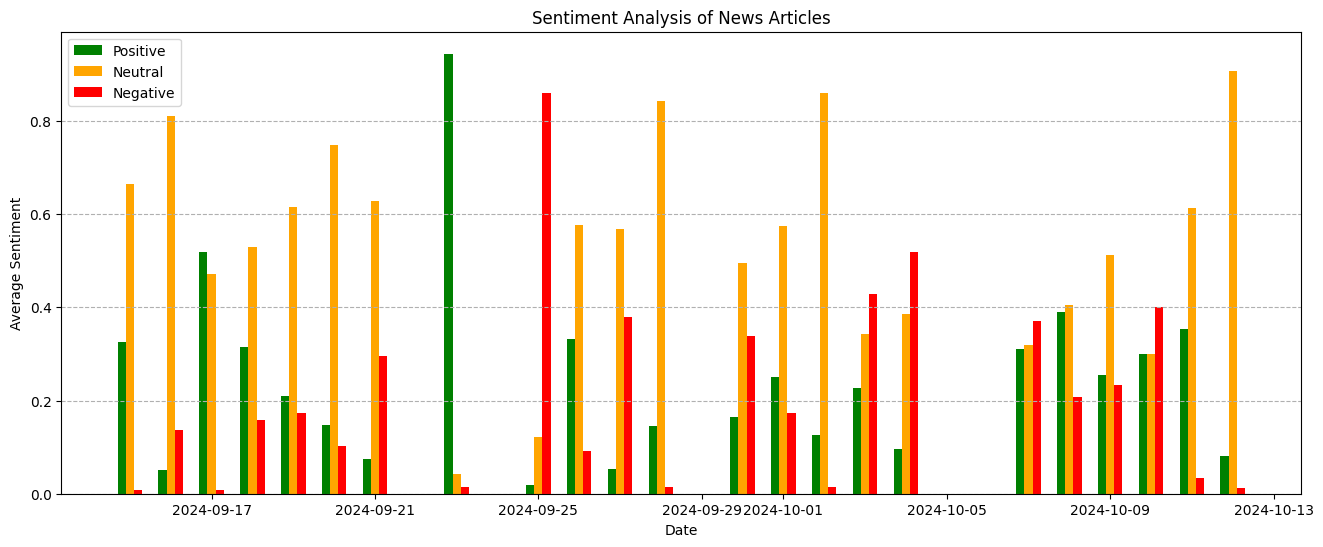
\includegraphics[width=0.85\linewidth]{gfx/m5l2_img001.png}
\par\smallskip{\small \textbf{Hình:} Cảm xúc trung bình của các bài báo theo ngày (tích cực, tiêu cực, trung lập).}
\end{figure}

Biểu đồ thu được là biểu đồ cột thể hiện cảm xúc trung bình của các bài báo theo thời gian. Mỗi ngày có ba cột, đại diện cho ba loại cảm xúc: tích cực (xanh lá), tiêu cực (đỏ) và trung lập (cam). Chiều cao của mỗi cột cho biết độ lớn của điểm cảm xúc trung bình thuộc loại đó vào ngày tương ứng. Cột càng cao thì cảm xúc càng mạnh.

Biểu đồ cho phép chúng ta quan sát xu hướng cảm xúc theo thời gian. Chúng ta có thể thấy cảm xúc trung bình thay đổi như thế nào qua các ngày, tức là đang trở nên tích cực hơn, tiêu cực hơn hay giữ ở mức trung lập. Bằng cách so sánh chiều cao các cột của từng loại, chúng ta có thể xác định những giai đoạn có cảm xúc tích cực hoặc tiêu cực mạnh hơn. Chẳng hạn, nếu vào một ngày nào đó cột đỏ (tiêu cực) cao hơn nhiều so với cột xanh lá (tích cực), điều này cho thấy các bài báo của ngày đó nhìn chung mang cảm xúc tiêu cực hơn. Ngược lại, cột xanh lá cao hơn sẽ cho thấy cảm xúc tích cực hơn.

\subsection{Điểm phân tích cảm xúc kết hợp với giá cổ phiếu}

Hãy xem xét ví dụ sau để thấy cách sử dụng điểm phân tích cảm xúc kết hợp với giá cổ phiếu của Microsoft, đồng thời lưu ý các hạn chế về độ chính xác của phân tích cảm xúc và nhu cầu sử dụng thêm các công cụ phân tích khác.

Trong ví dụ này, chúng ta sẽ trực quan hóa xu hướng của cảm xúc và giá. Chúng ta sẽ vẽ điểm cảm xúc cùng với giá cổ phiếu lịch sử. Điều này có thể giúp nhận diện bằng mắt thường những tương quan tiềm năng giữa các thay đổi về cảm xúc và biến động giá.

\begin{lstlisting}[language=Python,escapeinside={(*@}{@*)}]
# Fetch Microsoft stock data for the same date range
msft = yf.download("MSFT", start=df_grouped.index.min(), end=df_grouped.index.max())

# Scale the Microsoft price data
scaler = MinMaxScaler()
scaled_stock_price = scaler.fit_transform(msft[['Close']])

# Plot scaled price plot
fig, ax = plt.subplots(figsize=(16, 6))
ax.plot(msft.index, scaled_stock_price, color='blue', label='MSFT Adj Close Price (Scaled)')

# Plot the sentiment data
width = 0.2  # Adjust the width as needed
ax.bar(df_grouped.index - pd.DateOffset(days=width), df_grouped['avg_negative'], width=width, label='Negative', color='red')
ax.bar(df_grouped.index, df_grouped['avg_neutral'], width=width, label='Neutral', color='orange')
ax.bar(df_grouped.index + pd.DateOffset(days=width), df_grouped['avg_positive'], width=width, label='Positive', color='green')

# Set plot attributes (labels, ticks, title, legend, gridlines)
ax.set_xlabel('Date')
ax.set_title('Sentiment Analysis and Stock Price of Microsoft (scaled)')
ax.set_ylabel('Value (Sentiment and Stock Price)')
ax.legend()
ax.grid(True, axis='y', linestyle='--')
plt.show()
\end{lstlisting}

Giờ đây biểu đồ cũng hiển thị giá cổ phiếu của Microsoft cùng với các cột điểm cảm xúc. Lưu ý rằng giá cổ phiếu đã được chuẩn hóa tỷ lệ, và chúng ta thực hiện việc này bằng MinMaxScaler. MinMaxScaler từ \texttt{sklearn.preprocessing} đưa dữ liệu về một khoảng giá trị xác định, thường là từ 0 đến 1. Nó thực hiện điều này bằng cách áp dụng công thức sau:

\[X_{\text{scaled}} = \frac{(X - X_{min})}{(X_{max} - X_{min})}\]

Trong đó:

\begin{itemize}
\item
  \(X\) là dữ liệu gốc;
\item
  \(X_{\text{scaled}}\) là dữ liệu đã chuẩn hóa tỷ lệ;
\item
  \(X_{min}\) là giá trị nhỏ nhất của mỗi đặc trưng (cột) trong \(X\);
\item
  \(X_{max}\) là giá trị lớn nhất của mỗi đặc trưng (cột) trong \(X\);
\end{itemize}

Điều này có nghĩa là điểm dữ liệu có giá trị lớn nhất trong dữ liệu gốc sẽ được chuẩn hóa thành 1. Điểm dữ liệu có giá trị nhỏ nhất trong dữ liệu gốc sẽ được chuẩn hóa thành 0. Và tất cả các điểm dữ liệu còn lại sẽ được chuẩn hóa theo tỷ lệ giữa 0 và 1 dựa trên vị trí tương đối của chúng trong khoảng giá trị của dữ liệu gốc.

Mặc dù giá cổ phiếu đã chuẩn hóa không cho thấy các giá trị giá thực tế, nó vẫn biểu diễn biến động giá cổ phiếu theo cách đã được chuẩn hóa, cho phép chúng ta tập trung vào các xu hướng và mô hình, đồng thời so sánh chúng với các đặc trưng đã chuẩn hóa khác. Khi vẽ giá cổ phiếu đã chuẩn hóa cùng với điểm cảm xúc, về bản chất chúng ta đang so sánh các xu hướng và mô hình của cả hai đặc trưng theo thời gian. Chúng ta có thể quan sát xem cảm xúc tích cực có xu hướng trùng với các biến động giá tăng hay không, cảm xúc tiêu cực có trùng với các biến động giảm hay không, hoặc liệu có bất kỳ mối quan hệ thú vị nào khác.

\section{Kịch bản: Mô hình hóa chủ đề của tin tức tài chính}

Giờ đây, chúng ta sẽ sử dụng dữ liệu từ News API để khám phá các chủ đề tiềm ẩn trong các bài báo tài chính liên quan đến Microsoft và phân tích cảm xúc gắn với từng chủ đề.

\textbf{Mô hình hóa chủ đề} (topic modeling) là một kỹ thuật học máy không giám sát dùng để khám phá các cấu trúc chủ đề hay các chủ đề tiềm ẩn trong một tập hợp văn bản (còn gọi là \textbf{kho ngữ liệu}, corpus). Kỹ thuật này nhằm tự động nhận diện các nhóm từ thường xuyên xuất hiện cùng nhau trong các văn bản, đại diện cho những chủ đề hoặc nội dung nền tảng. Các thuật toán mô hình hóa chủ đề thường hoạt động dựa trên giả định rằng mỗi văn bản là sự pha trộn của một số ít chủ đề, và mỗi chủ đề được đặc trưng bởi một phân phối của các từ. Mục tiêu là học các phân phối chủ đề này cùng với việc gán chủ đề cho từng văn bản.

Các thuật ngữ chính:

\begin{itemize}
\item
  \textbf{Văn bản (Document):} Một đơn vị văn bản đơn lẻ, chẳng hạn như một bài báo, một bài đăng blog hoặc một tweet.
\item
  \textbf{Kho ngữ liệu (Corpus):} Một tập hợp các văn bản.
\item
  \textbf{Chủ đề (Topic):} Một cấu trúc chủ đề tiềm ẩn trong kho ngữ liệu, được biểu diễn bằng một phân phối của các từ.
\item
  \textbf{Phân phối văn bản-chủ đề (Document-Topic Distribution):} Xác suất hoặc trọng số của từng chủ đề trong mỗi văn bản.
\item
  \textbf{Phân phối chủ đề-từ (Topic-Word Distribution):} Xác suất hoặc trọng số của từng từ trong mỗi chủ đề.
\end{itemize}

Phân rã ma trận không âm (NMF) là một kỹ thuật mạnh mẽ để khám phá các chủ đề tiềm ẩn trong dữ liệu văn bản. Khi áp dụng vào tin tức tài chính, chúng ta có thể phát hiện các chủ đề chính đang được thảo luận về Microsoft. Việc kết hợp mô hình hóa chủ đề với phân tích cảm xúc giúp hiểu sâu hơn về cảm xúc gắn với các chủ đề khác nhau. Điều này có thể giúp xác định những lĩnh vực mà công ty nhận được nhận định tích cực hoặc tiêu cực. Những hiểu biết thu được từ phân tích này có thể hỗ trợ các quyết định đầu tư, quản trị rủi ro và chiến lược quan hệ công chúng.

\textbf{Các bước triển khai:}

\begin{itemize}
\item
  \textbf{Chuẩn bị dữ liệu:} Chúng ta sẽ sử dụng DataFrame \texttt{df} hiện có chứa dữ liệu News API, chọn cột \textquotesingle Description\textquotesingle{} làm dữ liệu văn bản để phân tích. Chúng ta sẽ tiền xử lý dữ liệu văn bản (loại bỏ từ dừng, dấu câu, rút gọn gốc từ/chuẩn hóa từ vựng).
\item
  \textbf{Tạo ma trận văn bản-thuật ngữ (TDM):} Sau đó, chúng ta sẽ tạo ma trận văn bản-thuật ngữ bằng TF-IDF (Term Frequency-Inverse Document Frequency). Ma trận này biểu diễn tần suất hoặc mức độ quan trọng của từng từ trong mỗi văn bản.
\item
  \textbf{Áp dụng NMF:} Chúng ta áp dụng NMF lên ma trận văn bản-thuật ngữ để phân rã thành hai ma trận: ma trận \(W\) biểu diễn mức độ quan trọng của từng chủ đề trong mỗi văn bản và ma trận \(H\) biểu diễn mức độ quan trọng của từng từ trong mỗi chủ đề.
\item
  \textbf{Trích xuất và diễn giải chủ đề:} Truy cập ma trận chủ đề-từ (\(H\)) để xem xét các từ hàng đầu của từng chủ đề. Xác định các từ có trọng số cao nhất trong mỗi hàng của \(H\) để hiểu nội dung của từng chủ đề. Dựa trên các từ hàng đầu, chúng ta đặt tên có ý nghĩa cho các chủ đề để dễ diễn giải.
\item
  \textbf{Gán chủ đề cho văn bản:} Lấy ma trận văn bản-chủ đề (\(W\)) để gán chủ đề chiếm ưu thế cho các văn bản. Với mỗi văn bản, chúng ta tìm chủ đề có trọng số cao nhất trong hàng tương ứng của \(W\). Cách này gán chủ đề nổi bật nhất cho mỗi văn bản.
\end{itemize}

\subsection{Chuẩn bị dữ liệu}

Chúng ta bắt đầu với bước chuẩn bị dữ liệu. Chúng ta tiền xử lý cột \textquotesingle Description\textquotesingle{} bằng hàm \texttt{preprocess()} đã giới thiệu ở trên và lưu mỗi mô tả đã xử lý vào một cột mới có tên \textquotesingle Processed\_Description\textquotesingle:

\begin{lstlisting}[language=Python,escapeinside={(*@}{@*)}]
# Preprocessing 'Description' column in df
df.loc[:, 'Processed_Description'] = df['Description'].apply(lambda x: preprocess(x))
\end{lstlisting}

Sau đó, chúng ta sẵn sàng áp dụng kỹ thuật Tần suất từ - Nghịch đảo tần suất văn bản (Term Frequency-Inverse Document Frequency, TF-IDF).

\subsection{Trích xuất đặc trưng - Ma trận tài liệu-thuật ngữ (TDM)}

Trong đoạn mã sau, chúng ta khớp (fit) bộ vector hóa \texttt{TfidfVectorizer} với dữ liệu trong cột \textquotesingle Processed\_Description\textquotesingle. Chúng ta áp dụng \texttt{TfidfVectorizer} với tham số \texttt{max\_features=250}, giới hạn kích thước từ vựng ở 250 từ xuất hiện thường xuyên nhất. Điều này giúp giảm số chiều của ma trận tài liệu-thuật ngữ (DTM) và có thể cải thiện hiệu năng. Chúng ta cũng dùng tham số \texttt{stop\_words=\textquotesingle{}english\textquotesingle{}} để loại bỏ các từ tiếng Anh thông dụng (như "the," "a," "is") khỏi từ vựng, vì chúng thường không mang nhiều thông tin có ý nghĩa. Thao tác này sẽ chuyển dữ liệu văn bản trong \textquotesingle Processed\_Description\textquotesingle{} thành ma trận tài liệu-thuật ngữ (DTM), được biểu diễn bằng biến \texttt{dtm}:

\begin{lstlisting}[language=Python,escapeinside={(*@}{@*)}]
# TF-IDF Vectorization
vectorizer = TfidfVectorizer(max_features=250, stop_words='english')
dtm = vectorizer.fit_transform(df['Processed_Description'])
dtm.shape
\end{lstlisting}

Biến \texttt{dtm} lúc này chứa một ma trận thưa, trong đó:

\begin{itemize}
\item
  Mỗi hàng đại diện cho một tài liệu (trong trường hợp của chúng ta là một bài báo tin tức).
\item
  Mỗi cột đại diện cho một từ (hay đặc trưng) trong từ vựng.
\item
  Các giá trị trong ma trận biểu thị điểm TF-IDF của từng từ trong từng tài liệu.
\item
  \texttt{dtm} thường được lưu dưới dạng ma trận thưa để tiết kiệm bộ nhớ vì nó thường chứa nhiều giá trị bằng không.
\end{itemize}

Phạm vi thông thường của \texttt{max\_features} là từ 1000 đến 5000, nhưng có thể thay đổi rất nhiều tùy theo tập dữ liệu và tác vụ, dựa trên các yếu tố như kích thước tập dữ liệu, độ phức tạp của tác vụ, tài nguyên tính toán, thực nghiệm, v.v. Với một tập dữ liệu như của chúng ta chỉ có khoảng 90 hàng, giá trị \texttt{max\_features} từ 100 đến 500 có lẽ là điểm khởi đầu phù hợp để cân bằng giữa số chiều và lượng thông tin.

\subsection{Áp dụng NMF}

Sau khi tạo \texttt{dtm}, giờ đây chúng ta có thể áp dụng NMF lên ma trận này để khám phá các chủ đề tiềm ẩn trong các bài báo tin tức tài chính. Chúng ta sẽ thực hiện việc này với tham số \texttt{n\_components=5}, tham số quy định số lượng chủ đề (hay thành phần) mà ta muốn trích xuất từ dữ liệu. Trong trường hợp này, ta nhắm đến năm chủ đề. \texttt{random\_state=42} đặt một hạt giống ngẫu nhiên (random seed) để đảm bảo khả năng tái lập kết quả. Việc dùng cùng một hạt giống bảo đảm ta thu được cùng một kết quả mỗi lần chạy mã:

\begin{lstlisting}[language=Python,escapeinside={(*@}{@*)}]
# NMF
nmf_model = NMF(n_components=5, random_state=42) # 5 topics
W = nmf_model.fit_transform(dtm)
H = nmf_model.components_
\end{lstlisting}

NMF được dùng để khám phá các chủ đề tiềm ẩn trong dữ liệu văn bản. Phương pháp này phân rã ma trận tài liệu-thuật ngữ thành hai ma trận có số chiều thấp hơn, biểu diễn mối quan hệ giữa từ và chủ đề, cũng như giữa chủ đề và tài liệu. Giờ đây chúng ta đã thu được:

\begin{itemize}
\item
  \(W\) (Ma trận Tài liệu-Chủ đề) biểu diễn phân phối của các chủ đề trong từng tài liệu. Mỗi hàng của \(W\) tương ứng với một tài liệu trong kho ngữ liệu, và mỗi cột tương ứng với một chủ đề do NMF khám phá. Các giá trị trong \(W\) cho biết trọng số hay xác suất xuất hiện của từng chủ đề trong mỗi tài liệu.
\item
  \(H\) (Ma trận Chủ đề-Từ) biểu diễn phân phối của các từ trong từng chủ đề. Mỗi hàng của \(H\) tương ứng với một chủ đề, và mỗi cột tương ứng với một từ trong từ vựng. Các giá trị trong \(H\) cho biết trọng số hay mức độ quan trọng của từng từ trong mỗi chủ đề.
\end{itemize}

Tham số \texttt{n\_components=5} xác định số lượng chủ đề (hay thành phần) mà ta muốn trích xuất từ dữ liệu. Trong trường hợp của chúng ta, ta nhắm đến việc khám phá năm chủ đề riêng biệt trong các bài báo tin tức tài chính liên quan đến Microsoft. Số lượng chủ đề nhỏ (như năm) thường cho kết quả dễ diễn giải hơn. Việc hiểu và gán nhãn có ý nghĩa cho năm chủ đề dễ dàng hơn so với, chẳng hạn, 20 hay 50 chủ đề. Khi mới bắt đầu với mô hình hóa chủ đề, thông thường nên bắt đầu với số lượng chủ đề nhỏ rồi tăng dần nếu cần. Cách này giúp nắm được bức tranh tổng quát về các chủ đề chính trong dữ liệu trước khi đi vào phân tích chi tiết hơn. Số lượng chủ đề nhỏ cũng làm giảm chi phí tính toán của NMF, giúp quá trình nhanh hơn, đặc biệt với các tập dữ liệu lớn hơn.

\subsection{Trích xuất và diễn giải chủ đề}

Bây giờ, chúng ta hãy xem xét các từ hàng đầu trong mỗi chủ đề để hiểu nội dung của chủ đề đó. Mục tiêu là hiểu các nội dung hay đối tượng mà năm chủ đề do NMF trích xuất đại diện.

Hãy nhớ rằng ma trận \(H\) lưu trữ trọng số của mỗi từ trong mỗi chủ đề. Chúng ta muốn xác định các từ có trọng số cao nhất cho từng chủ đề, vì những từ này đại diện tốt nhất cho nội dung của chủ đề. Với mỗi chủ đề, chúng ta sẽ hiển thị \(n\) từ hàng đầu có trọng số cao nhất. Điều này cho ta một cái nhìn sơ lược về đề tài của chủ đề. Dựa trên các từ hàng đầu, chúng ta sẽ cố gắng gán một nhãn hoặc cách diễn giải có ý nghĩa cho từng chủ đề. Việc này đòi hỏi kiến thức chuyên ngành và sự cân nhắc kỹ lưỡng về bối cảnh của các bài báo tin tức tài chính.

\begin{lstlisting}[language=Python,escapeinside={(*@}{@*)}]
# Retrieves the names of the features (words)
feature_names = vectorizer.get_feature_names_out()

# Extract top words
n_top_words = 10  # Top 10 words
for topic_idx, topic in enumerate(H):
    print(f"\nTopic {topic_idx + 1}:")
    print(" ".join([feature_names[i]
                    for i in topic.argsort()[:-n_top_words - 1:-1]]))
\end{lstlisting}

Chúng ta cũng có thể vẽ biểu đồ các từ hàng đầu của từng chủ đề để trực quan hóa tốt hơn. Trong đoạn mã sau, chúng ta vẽ 10 từ hàng đầu của mỗi chủ đề dưới dạng các biểu đồ cột con:

\begin{lstlisting}[language=Python,escapeinside={(*@}{@*)}]
# Set figure size
fig, axes = plt.subplots(1, nmf_model.n_components, figsize=(16, 6), sharex=True)
axes = axes.flatten()  # Convert to 1D array for easier indexing

# Plot bar subplots for each topic
for topic_idx, topic in enumerate(H):
    top_features_ind = topic.argsort()[:-n_top_words - 1:-1]
    top_features = [feature_names[i] for i in top_features_ind]
    weights = topic[top_features_ind]

    ax = axes[topic_idx]
    ax.barh(top_features, weights, height=0.5, fill='blue')
    ax.set_title(f'Topic {topic_idx + 1}', fontdict={'fontsize': 14})
    ax.invert_yaxis()
    ax.tick_params(axis='both', which='major', labelsize=12)

# Set figure attributes (title)
fig.suptitle('Top words in topics in NMF model', fontsize=20, y=0.98)
fig.tight_layout(h_pad=2.0)
plt.show()
\end{lstlisting}

Mục đích chính của đoạn mã này là hiển thị các từ hàng đầu của từng chủ đề do NMF trích xuất. Điều này giúp diễn giải các chủ đề và hiểu những nội dung hay đối tượng mà chúng đại diện.

Tại thời điểm viết bài, chúng tôi thu được các từ hàng đầu sau cho từng chủ đề (bạn có thể nhận được kết quả khác vì News API sẽ có một tập bài báo khác vào lúc bạn chạy đoạn mã này):

\begin{itemize}
\item
  \textbf{Chủ đề 1: Microsoft Windows và các tính năng AI}

  \begin{itemize}
    \item
    Từ hàng đầu: \texttt{copilot,\ plus,\ feature,\ new,\ pcs,\ features,\ search,\ voice,\ ai,\ windows}
  \item
    Diễn giải: Chủ đề này dường như liên quan đến các tính năng và cải tiến mới trong Microsoft Windows, đặc biệt là những tính năng liên quan đến AI và khả năng tìm kiếm bằng giọng nói. Copilot, một trợ lý AI mới có thể xuất hiện, cũng là một nội dung nổi bật.
  \end{itemize}
\item
  \textbf{Chủ đề 2: Các trung tâm dữ liệu và sáng kiến năng lượng của Microsoft}

  \begin{itemize}
    \item
    Từ hàng đầu: \texttt{data,\ energy,\ centers,\ power,\ nuclear,\ ai,\ tech,\ run,\ microsoft,\ carbon}
  \item
    Diễn giải: Chủ đề này dường như tập trung vào các trung tâm dữ liệu của Microsoft và mức tiêu thụ năng lượng của chúng. Chủ đề có thể bao gồm các thảo luận về nguồn điện, trong đó có năng lượng hạt nhân, và các sáng kiến nhằm giảm phát thải carbon. Việc sử dụng công nghệ AI trong các trung tâm dữ liệu cũng có thể là một nội dung đáng chú ý.
  \end{itemize}
\item
  \textbf{Chủ đề 3: Các nỗ lực AR/VR của Microsoft (Hololens)}

  \begin{itemize}
    \item
    Từ hàng đầu: \texttt{microsoft,\ windows,\ hololens,\ headsets,\ according,\ vr,\ update,\ production,\ uploadvr,\ 11}
  \item
    Diễn giải: Chủ đề này có khả năng xoay quanh các nỗ lực về thực tế tăng cường và thực tế ảo của Microsoft, đặc biệt tập trung vào kính Hololens. Chủ đề có thể bao gồm các cập nhật về sản xuất Hololens, các tính năng mới, hoặc quan hệ hợp tác với các nền tảng liên quan đến VR như UploadVR.
  \end{itemize}
\item
  \textbf{Chủ đề 4: Cạnh tranh trong lĩnh vực AI (Microsoft, OpenAI, Google)}

  \begin{itemize}
    \item
    Từ hàng đầu: \texttt{openai,\ google,\ ai,\ microsoft,\ stay,\ date,\ financial,\ way,\ competition,\ amid}
  \item
    Diễn giải: Chủ đề này xoay quanh sự cạnh tranh trong lĩnh vực trí tuệ nhân tạo, chủ yếu liên quan đến Microsoft, OpenAI và Google. Chủ đề có thể thảo luận về các khía cạnh tài chính, quan hệ đối tác chiến lược và bức tranh tổng thể của cuộc đua AI.
  \end{itemize}
\item
  \textbf{Chủ đề 5: Microsoft Flight Simulator và trò chơi điện tử}

  \begin{itemize}
    \item
    Từ hàng đầu: \texttt{flight,\ game,\ simulator,\ microsoft,\ 2024,\ test,\ based,\ reboot,\ 2020,\ office}
  \item
    Diễn giải: Chủ đề này dường như liên quan đến Microsoft Flight Simulator, một trò chơi mô phỏng bay phổ biến. Chủ đề có thể bao gồm các thảo luận về bản cập nhật, tính năng mới, các giai đoạn thử nghiệm hoặc những bản phát hành tiềm năng trong tương lai. Việc xuất hiện từ "office" hơi bất thường và có thể cần thêm ngữ cảnh để hiểu mức độ liên quan của nó.
  \end{itemize}
\end{itemize}

Dựa trên các diễn giải này, dưới đây là một bộ nhãn được đề xuất cho các chủ đề:

\begin{enumerate}
\def\labelenumi{\arabic{enumi}.}
\item
  Cải tiến AI trong Windows
\item
  Tính bền vững của trung tâm dữ liệu
\item
  Hololens và AR/VR
\item
  Cạnh tranh trong ngành AI
\item
  Flight Simulator và trò chơi điện tử
\end{enumerate}

Các nhãn này thể hiện ngắn gọn và đầy đủ thông tin các nội dung mà từng chủ đề nắm bắt được. Hãy nhớ rằng việc diễn giải chủ đề có thể mang tính chủ quan, vì vậy các nhãn có thể được điều chỉnh dựa trên cách hiểu của riêng bạn về dữ liệu và bối cảnh.

Bằng cách phân tích cẩn thận các từ hàng đầu và xem xét bối cảnh rộng hơn, chúng ta có thể thu được những hiểu biết giá trị về các nội dung chính được thảo luận trong các bài báo tin tức tài chính liên quan đến Microsoft.

\subsection{Gán chủ đề cho tài liệu}

Bây giờ, chúng ta sẽ dùng \texttt{W} để gán chủ đề nổi bật nhất cho từng tài liệu. Ta có thể thực hiện bằng cách tìm chủ đề (cột) có trọng số cao nhất đối với mỗi tài liệu (hàng) trong \texttt{W}:

\begin{lstlisting}[language=Python,escapeinside={(*@}{@*)}]
# Assigns the dominant topic for each document
df['Dominant_Topic'] = W.argmax(axis=1) + 1  # +1 to start topic numbering from 1
\end{lstlisting}

Ở đây, \texttt{W.argmax(axis=1)} tìm chỉ số của giá trị lớn nhất (trọng số cao nhất) trong mỗi hàng của \(W\). Chỉ số này tương ứng với chủ đề chiếm ưu thế của tài liệu đó. Còn \texttt{+\ 1} cộng thêm 1 vào chỉ số chủ đề để việc đánh số chủ đề bắt đầu từ 1 thay vì 0 (mặc định trong cách đánh chỉ số của Python).

Biểu đồ cột có thể được dùng để trực quan hóa phân phối các chủ đề trong từng tài liệu riêng lẻ hoặc trên toàn bộ kho ngữ liệu. Biểu đồ cột sau đây thể hiện phân phối chủ đề trung bình trên tất cả các tài liệu:

\begin{lstlisting}[language=Python,escapeinside={(*@}{@*)}]
# Visualize average topic distribution across all documents
avg_topic_distribution = W.mean(axis=0)

# Define topic labels
topic_labels = ["Windows AI Enhancements", "Data Center Sustainability",
                "Hololens and AR/VR", "AI Industry Competition",
                "Flight Simulator and Gaming"]

# Create bar plot
bars = plt.bar(np.arange(nmf_model.n_components) + 1, avg_topic_distribution, color='skyblue')

# Add bar labels inside bars
for bar, label in zip(bars, topic_labels):
    plt.text(bar.get_x() + bar.get_width() / 2, bar.get_height() / 2, label,
             ha='center', va='center', rotation=90, color='black', fontsize=8)

plt.xticks(np.arange(nmf_model.n_components) + 1)
plt.xlabel("Topic")
plt.ylabel("Average Weight")
plt.title("Average Topic Distribution Across All Documents")
plt.show()
\end{lstlisting}

Biểu đồ cột này minh họa mức độ phổ biến trung bình của từng chủ đề trên tất cả các tài liệu trong tập dữ liệu. Chiều cao của mỗi cột biểu thị trọng số trung bình, hay mức độ quan trọng, của chủ đề đó trên toàn bộ các tài liệu được phân tích. Cột càng cao cho thấy chủ đề đó càng nổi bật hoặc được đề cập thường xuyên hơn xét trên tổng thể.

Dựa vào chiều cao của các cột tương ứng, ta có thể thấy "AI Industry Competition" là chủ đề phổ biến nhất, tiếp theo là "Hololens and AR/VR".

Thông qua việc xem xét trực quan hóa này, chúng ta có thể hiểu rõ hơn về phân bố chủ đề tổng thể trong tập dữ liệu. Thông tin này sẽ định hướng cho các phân tích tiếp theo, chẳng hạn tập trung vào các tài liệu liên quan đến "AI Industry Competition" và "Hololens and AR/VR" để hiểu sâu hơn về những chủ đề chủ đạo này.

\section{Kết luận}

Trong bài học này, chúng ta đã khảo sát các nguồn dữ liệu tin tức khác nhau. Chúng ta đã so sánh và đối chiếu các nguồn như yfinance, Google News RSS và News API. Cuối cùng, News API được lựa chọn nhờ tính linh hoạt và các tính năng của nó.

Sau đó, chúng ta thực hiện phân tích cảm xúc bằng FinBERT, một mô hình NLP được huấn luyện trước dành cho văn bản tài chính. Điểm số cảm xúc (tích cực, tiêu cực và trung lập) được tính cho các bài báo về Microsoft. Các điểm số cảm xúc được vẽ theo thời gian để quan sát xu hướng và các mối tương quan tiềm năng với giá cổ phiếu của Microsoft.

Cuối cùng, chúng ta áp dụng mô hình hóa chủ đề, sử dụng phân rã ma trận không âm (NMF) để khám phá các chủ đề hoặc nội dung chính tiềm ẩn trong dữ liệu tin tức. Quá trình này bao gồm tiền xử lý văn bản, tạo ma trận tài liệu-thuật ngữ bằng TF-IDF và áp dụng thuật toán NMF.

\begin{center}\rule{0.5\linewidth}{0.5pt}\end{center}

Bản quyền 2024 WorldQuant University. Nội dung này chỉ được cấp phép cho mục đích sử dụng cá nhân. Nghiêm cấm phân phối lại hoặc công bố tài liệu này.

\begin{lstlisting}[language=Python,escapeinside={(*@}{@*)}]

\end{lstlisting}

\chapter{Đọc thêm 1: FinBERT -- Phân tích cảm xúc tài chính bằng mô hình ngôn ngữ tiền huấn luyện (Araci)}
\label{ch:M5L2DocThem1}

\section{Thông tin nguồn}

\begin{itemize}
  \item \textbf{Nguồn:} Araci, D. ``FinBERT: Financial Sentiment Analysis with Pre-trained Language Models.'' arXiv:1908.10063, 2019.
  \item \textbf{Phần cần đọc:} Toàn bộ bài báo (11 trang)
  \item \textbf{Ghi chú:} bản chuyển ngữ tiếng Việt súc tích, bám cấu trúc nguồn (giữ nguyên tiêu đề, công thức, số liệu, bảng, chú thích và danh mục tài liệu tham khảo).
\end{itemize}

FinBERT: Phân tích cảm xúc tài chính bằng các mô hình ngôn ngữ tiền huấn luyện

arXiv:1908.10063v1 {[}cs.CL{]} 27 Aug 2019

Luận văn nộp một phần yêu cầu để lấy bằng thạc sĩ khoa học --- Dogu Araci (12255068), ngành Nghiên cứu thông tin, chuyên ngành Khoa học dữ liệu, Khoa Khoa học, Đại học Amsterdam, 2019-06-25.

{\small
\begin{longtable}[]{@{}
  >{\raggedright\arraybackslash}p{(\columnwidth - 6\tabcolsep) * \real{0.2500}}
  >{\raggedright\arraybackslash}p{(\columnwidth - 6\tabcolsep) * \real{0.2500}}
  >{\raggedright\arraybackslash}p{(\columnwidth - 6\tabcolsep) * \real{0.2500}}
  >{\raggedright\arraybackslash}p{(\columnwidth - 6\tabcolsep) * \real{0.2500}}@{}}
\toprule\noalign{}
\begin{minipage}[b]{\linewidth}\raggedright
Vai trò
\end{minipage} & \begin{minipage}[b]{\linewidth}\raggedright
Họ tên
\end{minipage} & \begin{minipage}[b]{\linewidth}\raggedright
Đơn vị
\end{minipage} & \begin{minipage}[b]{\linewidth}\raggedright
Email
\end{minipage} \\
\midrule\noalign{}
\endhead
\bottomrule\noalign{}
\endlastfoot
Người hướng dẫn nội bộ & Dr Pengjie Ren & UvA, ILPS & p.ren@uva.nl \\
Người hướng dẫn bên ngoài & Dr Zulkuf Genc & Naspers Group & zulkuf.genc@naspers.com \\
\end{longtable}
}

FinBERT: Phân tích cảm xúc tài chính bằng các mô hình ngôn ngữ tiền huấn luyện

Dogu Tan Araci, dogu.araci@student.uva.nl, University of Amsterdam, Amsterdam, Hà Lan

\subsection{TÓM TẮT}

Các phương pháp học chuyển giao (transfer learning) trong xử lý ngôn ngữ tự nhiên (NLP) là giải pháp đầy triển vọng cho cả hai thách thức nêu trên và là trọng tâm của luận văn. Ý tưởng cốt lõi: huấn luyện mô hình ngôn ngữ trên các kho ngữ liệu rất lớn, rồi khởi tạo các mô hình tác vụ hạ nguồn bằng trọng số học được từ tác vụ mô hình hóa ngôn ngữ, nhờ đó đạt hiệu năng tốt hơn nhiều. Phần được khởi tạo có thể chỉ là một lớp nhúng từ (word embedding) {[}23{]} hoặc toàn bộ mô hình {[}5{]}. Về lý thuyết, cách này giải quyết bài toán khan hiếm dữ liệu có nhãn: mô hình ngôn ngữ không cần nhãn vì tác vụ là dự đoán từ tiếp theo, và vẫn học được cách biểu diễn thông tin ngữ nghĩa. Khi đó, bước tinh chỉnh (fine-tune) trên dữ liệu có nhãn chỉ còn phải học cách dùng thông tin ngữ nghĩa này để dự đoán nhãn.

Một thành phần đặc thù của học chuyển giao là khả năng tiếp tục tiền huấn luyện mô hình ngôn ngữ trên kho ngữ liệu không nhãn thuộc lĩnh vực cụ thể. Nhờ vậy mô hình học được các quan hệ ngữ nghĩa trong văn bản của lĩnh vực đích, vốn có khả năng phân phối khác với kho ngữ liệu tổng quát. Cách tiếp cận này đặc biệt hứa hẹn với lĩnh vực ngách như tài chính, nơi ngôn ngữ và từ vựng khác biệt rất lớn so với ngôn ngữ thông thường.

Mục tiêu của luận văn là kiểm chứng các ưu thế được giả định của việc sử dụng và tinh chỉnh mô hình ngôn ngữ tiền huấn luyện cho lĩnh vực tài chính. Để làm vậy, luận văn dự đoán cảm xúc của một câu trong bài báo tài chính đối với chủ thể tài chính được nhắc đến trong câu, sử dụng Financial PhraseBank do Malo et al. (2014) {[}17{]} xây dựng và tập dữ liệu chấm điểm cảm xúc FiQA Task 1 {[}15{]}.

Các đóng góp chính của luận văn như sau:

Phân tích cảm xúc tài chính là tác vụ khó do ngôn ngữ chuyên biệt và thiếu dữ liệu có nhãn trong lĩnh vực này. Các mô hình đa dụng kém hiệu quả vì ngôn ngữ tài chính chuyên biệt. Giả thuyết của chúng tôi là mô hình ngôn ngữ tiền huấn luyện giúp giải quyết vấn đề, vì cần ít ví dụ có nhãn hơn và có thể huấn luyện thêm trên kho ngữ liệu chuyên ngành. Chúng tôi giới thiệu FinBERT, mô hình ngôn ngữ dựa trên BERT, cho các tác vụ NLP tài chính. Kết quả cho thấy cải thiện ở mọi chỉ số đo được so với kết quả tốt nhất hiện nay (state-of-the-art) trên hai tập dữ liệu phân tích cảm xúc tài chính. Ngay cả với tập huấn luyện nhỏ hơn và chỉ tinh chỉnh một phần mô hình, FinBERT vẫn vượt các phương pháp học máy tốt nhất hiện có.

\section{1 GIỚI THIỆU}

Giá trong thị trường mở phản ánh toàn bộ thông tin sẵn có về các tài sản được giao dịch trong nền kinh tế {[}16{]}. Khi có thông tin mới, mọi chủ thể cập nhật vị thế và giá điều chỉnh theo, khiến việc liên tục đánh bại thị trường là bất khả thi. Tuy nhiên, định nghĩa "thông tin mới" có thể thay đổi khi xuất hiện các công nghệ truy xuất thông tin mới, và việc sớm áp dụng chúng có thể mang lại lợi thế ngắn hạn.

Phân tích văn bản tài chính (tin tức, báo cáo phân tích, thông báo chính thức của công ty) là một nguồn thông tin mới tiềm năng. Lượng văn bản như vậy được tạo ra mỗi ngày chưa từng có, nên không một đơn vị nào đủ sức phân tích thủ công và rút ra thông tin khả dụng. Vì thế, phân tích cảm xúc hay độ phân cực (polarity) tự động của văn bản do các chủ thể tài chính tạo ra bằng các phương pháp NLP đã trở nên phổ biến trong thập kỷ qua {[}4{]}.

Mối quan tâm nghiên cứu chính của luận văn là phân tích độ phân cực, tức phân loại văn bản thành tích cực, tiêu cực hoặc trung lập trong một lĩnh vực cụ thể. Việc này phải giải quyết hai thách thức: 1) Các phương pháp phân loại tinh vi nhất dùng mạng nơ-ron cần lượng dữ liệu có nhãn rất lớn, mà gán nhãn văn bản tài chính đòi hỏi chuyên môn tốn kém. 2) Các mô hình phân tích cảm xúc huấn luyện trên kho ngữ liệu tổng quát không phù hợp, vì văn bản tài chính có ngôn ngữ chuyên biệt với từ vựng riêng và thường dùng cách diễn đạt mơ hồ thay vì các từ tích cực/tiêu cực dễ nhận biết.

Dùng các từ điển cảm xúc tài chính được xây dựng kỹ như Loughran và McDonald (2011) {[}11{]} có vẻ là giải pháp vì chúng đưa kiến thức tài chính sẵn có vào phân tích văn bản. Tuy nhiên, chúng dựa trên phương pháp "đếm từ", không đủ khả năng phân tích ý nghĩa ngữ nghĩa sâu hơn của văn bản.

\begin{itemize}
\item
  Giới thiệu FinBERT, một mô hình ngôn ngữ dựa trên BERT cho các tác vụ NLP tài chính, được đánh giá trên hai bộ dữ liệu phân tích cảm xúc tài chính.
\item
  Đạt kết quả tốt nhất hiện nay (state-of-the-art) trên FiQA sentiment scoring và Financial PhraseBank.
\item
  Triển khai thêm hai mô hình ngôn ngữ tiền huấn luyện khác là ULMFit và ELMo cho phân tích cảm xúc tài chính và so sánh với FinBERT.
\item
  Thực hiện các thí nghiệm khảo sát nhiều khía cạnh của mô hình: tác động của việc tiền huấn luyện thêm trên kho ngữ liệu tài chính, các chiến lược huấn luyện nhằm tránh quên thảm khốc (catastrophic forgetting), và chỉ tinh chỉnh một tập con nhỏ các lớp của mô hình để giảm thời gian huấn luyện mà hiệu năng không giảm đáng kể.
\end{itemize}

Phần còn lại của luận văn được cấu trúc như sau: trước hết, các nghiên cứu liên quan về phân tích phân cực (polarity) trong tài chính và về các mô hình ngôn ngữ tiền huấn luyện được thảo luận (Mục 2). Tiếp theo, các mô hình được đánh giá được mô tả (Mục 3), rồi đến thiết lập thí nghiệm (Mục 4). Mục 5 trình bày kết quả thí nghiệm trên các bộ dữ liệu cảm xúc tài chính. Mục 6 phân tích sâu hơn FinBERT từ nhiều góc độ. Cuối cùng, Mục 7 là kết luận.

\section{2 TÀI LIỆU LIÊN QUAN}

Phần này mô tả các nghiên cứu trước đây về phân tích cảm xúc trong tài chính (2.1) và phân loại văn bản bằng mô hình ngôn ngữ tiền huấn luyện (2.2).

\subsection{2.1 Phân tích cảm xúc trong tài chính}

Phân tích cảm xúc là tác vụ trích xuất cảm xúc hay quan điểm của con người từ ngôn ngữ viết {[}10{]}. Các nỗ lực gần đây chia làm hai nhóm: 1) phương pháp học máy với đặc trưng trích từ văn bản bằng "đếm từ" (word counting) {[}1, 19, 28, 30{]}; 2) phương pháp học sâu, trong đó văn bản được biểu diễn bằng chuỗi embedding {[}2, 25, 32{]}. Nhóm đầu không biểu diễn được thông tin ngữ nghĩa phát sinh từ một chuỗi từ cụ thể, còn nhóm sau thường bị coi là quá "khát dữ liệu" vì phải học số tham số lớn hơn nhiều {[}18{]}.

Phân tích cảm xúc tài chính khác phân tích cảm xúc thông thường không chỉ về lĩnh vực mà còn về mục đích: thường là đoán thị trường sẽ phản ứng thế nào với thông tin trong văn bản {[}9{]}. Loughran và McDonald (2016) tổng quan kỹ các công trình phân tích văn bản tài chính dùng học máy với cách tiếp cận "túi từ" (bag-of-words) hoặc phương pháp dựa trên từ điển {[}12{]}. Chẳng hạn, Loughran và McDonald (2011) xây dựng từ điển thuật ngữ tài chính gán các giá trị như "tích cực" hay "không chắc chắn" và đo sắc thái của tài liệu bằng cách đếm các từ có giá trị từ điển cụ thể {[}11{]}. Một ví dụ khác là Pagolu và cộng sự (2016), trong đó các n-gram từ tweet chứa thông tin tài chính được đưa vào các thuật toán học máy có giám sát để phát hiện cảm xúc đối với thực thể tài chính được nhắc đến.

Một trong những bài báo đầu tiên dùng học sâu cho phân tích phân cực văn bản tài chính là Kraus và Feuerriegel (2017) {[}7{]}. Họ áp dụng mạng nơ-ron LSTM lên các thông báo ad-hoc của công ty để dự đoán biến động thị trường chứng khoán và cho thấy phương pháp này chính xác hơn các phương pháp học máy truyền thống. Họ nhận thấy tiền huấn luyện mô hình trên kho ngữ liệu lớn hơn cải thiện kết quả; tuy nhiên việc tiền huấn luyện đó dùng tập dữ liệu có nhãn, là cách tiếp cận hạn chế hơn của chúng tôi, vì chúng tôi tiền huấn luyện mô hình ngôn ngữ như một tác vụ không giám sát.

Có nhiều công trình khác dùng các kiến trúc mạng nơ-ron khác nhau cho phân tích cảm xúc tài chính. Sohangir và cộng sự (2018) {[}26{]} áp dụng một số kiến trúc mạng nơ-ron thông dụng lên tập dữ liệu StockTwits và thấy CNN có hiệu quả nhất. Lutz và cộng sự (2018) {[}13{]} dùng doc2vec để tạo embedding câu trong thông báo ad-hoc của một công ty và dùng học đa thể hiện (multi-instance learning) để dự đoán kết quả thị trường chứng khoán. Maia và cộng sự (2018) {[}14{]} kết hợp đơn giản hóa văn bản và mạng LSTM để phân loại một tập câu từ tin tức tài chính theo cảm xúc, đạt kết quả state-of-the-art trên Financial PhraseBank, bộ dữ liệu cũng được dùng trong luận văn này.

Do thiếu các bộ dữ liệu tài chính có nhãn quy mô lớn, rất khó khai thác hết tiềm năng của mạng nơ-ron cho phân tích cảm xúc. Ngay cả khi các lớp đầu tiên (lớp nhúng từ) được khởi tạo bằng giá trị tiền huấn luyện, phần còn lại của mô hình vẫn phải học các quan hệ phức tạp từ lượng dữ liệu có nhãn tương đối nhỏ. Một giải pháp triển vọng hơn là khởi tạo gần như toàn bộ mô hình bằng giá trị tiền huấn luyện và tinh chỉnh các giá trị đó theo tác vụ phân loại.

\subsection{2.2 Phân loại văn bản bằng mô hình ngôn ngữ tiền huấn luyện}

Mô hình hóa ngôn ngữ là nhiệm vụ dự đoán từ tiếp theo trong một đoạn văn bản. Một bước tiến quan trọng gần đây của xử lý ngôn ngữ tự nhiên (NLP) là nhận ra rằng mô hình được huấn luyện cho bài toán mô hình hóa ngôn ngữ có thể được tinh chỉnh (fine-tune) thành công cho hầu hết các tác vụ NLP hạ nguồn chỉ với những sửa đổi nhỏ. Các mô hình này thường được huấn luyện trên kho ngữ liệu rất lớn, sau đó được bổ sung các lớp đặc thù cho tác vụ và tinh chỉnh trên tập dữ liệu mục tiêu {[}6{]}. Phân loại văn bản, trọng tâm của luận văn này, là một trường hợp ứng dụng hiển nhiên của cách tiếp cận đó.

ELMo (Embeddings from Language Models) {[}23{]} là một trong những ứng dụng thành công đầu tiên của cách tiếp cận này. Với ELMo, một mô hình ngôn ngữ hai chiều sâu được tiền huấn luyện trên kho ngữ liệu lớn; với mỗi từ, các trạng thái ẩn của mô hình được dùng để tính biểu diễn theo ngữ cảnh. Nhờ trọng số tiền huấn luyện của ELMo, có thể tính nhúng từ (word embeddings) theo ngữ cảnh cho bất kỳ đoạn văn bản nào. Việc khởi tạo embedding cho các tác vụ hạ nguồn bằng các nhúng này được chứng minh là cải thiện hiệu suất ở hầu hết tác vụ so với nhúng từ tĩnh như word2vec hay GloVe. Với các tác vụ phân loại văn bản như SST-5, ELMo đạt hiệu suất tiên tiến nhất (state-of-the-art) khi kết hợp với mạng phân loại bi-attentive {[}20{]}.

Dù ELMo tận dụng mô hình ngôn ngữ tiền huấn luyện để ngữ cảnh hóa biểu diễn, thông tin trích xuất từ mô hình ngôn ngữ vẫn chỉ hiện diện ở lớp đầu tiên của mô hình sử dụng nó. ULMFit (Universal Language Model Fine-tuning) {[}5{]} là công trình đầu tiên đạt được học chuyển giao (transfer learning) đúng nghĩa cho NLP, nhờ các kỹ thuật mới như tinh chỉnh phân biệt theo lớp (discriminative fine-tuning), tốc độ học tam giác nghiêng (slanted triangular learning rates) và rã đông dần (gradual unfreezing). Nhóm tác giả đã tinh chỉnh hiệu quả toàn bộ mô hình ngôn ngữ tiền huấn luyện cho phân loại văn bản. Họ cũng đề xuất tiền huấn luyện thêm mô hình ngôn ngữ trên kho ngữ liệu đặc thù lĩnh vực, với giả định dữ liệu của tác vụ đích có phân phối khác với kho ngữ liệu tổng quát mà mô hình ban đầu được huấn luyện.

Ý tưởng chính của ULMFit, tức tinh chỉnh hiệu quả mô hình ngôn ngữ tiền huấn luyện cho các tác vụ hạ nguồn, được nâng lên một tầm mới với Bidirectional Encoder Representations from Transformers (BERT) {[}3{]}, cũng là trọng tâm của bài báo này. BERT có hai điểm khác biệt quan trọng so với các mô hình trước: 1) BERT định nghĩa nhiệm vụ mô hình hóa ngôn ngữ là dự đoán các token bị che ngẫu nhiên trong chuỗi thay vì token tiếp theo, đồng thời thêm nhiệm vụ phân loại xem hai câu có nối tiếp nhau hay không. 2) BERT là mạng rất lớn, được huấn luyện trên kho ngữ liệu lớn chưa từng có. Hai yếu tố này giúp BERT đạt kết quả tiên tiến nhất trên nhiều tác vụ NLP như suy luận ngôn ngữ tự nhiên hay hỏi đáp.

Các chi tiết về tinh chỉnh BERT cho phân loại văn bản chưa được nghiên cứu kỹ. Một công trình gần đây là Sun et al. (2019) {[}27{]}, trong đó họ tiến hành chuỗi thí nghiệm về các cấu hình BERT khác nhau cho phân loại văn bản. Một số kết quả của họ sẽ được dẫn lại trong phần còn lại của luận văn để xác định cấu hình mô hình của chúng tôi.

3.1.4 Transformer. Transformer là kiến trúc dựa trên cơ chế chú ý (attention) để mô hình hóa thông tin tuần tự, là phương án thay thế cho mạng nơ-ron hồi quy (recurrent neural network) {[}29{]}. Nó được đề xuất như mô hình chuỗi-sang-chuỗi (sequence-to-sequence), nên gồm cơ chế bộ mã hóa (encoder) và bộ giải mã (decoder). Ở đây chỉ tập trung vào phần encoder (decoder khá tương tự). Encoder gồm nhiều lớp Transformer giống hệt nhau. Mỗi lớp có một lớp tự chú ý nhiều đầu (multi-headed self-attention) và một mạng truyền thẳng kết nối đầy đủ. Với mỗi lớp tự chú ý, ba ánh xạ từ embedding (key, query và value) được học. Từ key của mỗi token và các vector query của mọi token, điểm tương đồng được tính bằng tích vô hướng. Các điểm này được dùng để đặt trọng số cho các vector value nhằm thu được biểu diễn mới của token. Với tự chú ý nhiều đầu, các lớp này được nối lại với nhau để chuỗi được đánh giá từ nhiều "góc nhìn" khác nhau. Sau đó, các vector thu được đi qua các mạng kết nối đầy đủ với tham số dùng chung.

Như Vaswani 2017 {[}29{]} đã lập luận, kiến trúc Transformer có nhiều ưu điểm so với các cách tiếp cận dựa trên RNN. Do bản chất tuần tự, RNN khó song song hóa trên GPU hơn nhiều, và quá nhiều bước giữa các phần tử ở xa nhau trong chuỗi khiến thông tin khó được duy trì.

PHƯƠNG PHÁP

Trong phần này, chúng tôi trình bày bản triển khai BERT cho lĩnh vực tài chính có tên FinBERT, sau khi điểm qua nền tảng ngắn gọn về các kiến trúc mạng nơ-ron liên quan.

3.1 Kiến thức nền tảng

3.1.1 LSTM. Bộ nhớ dài-ngắn hạn (LSTM) là một loại mạng nơ-ron hồi quy cho phép các phụ thuộc dài hạn trong chuỗi được duy trì trong mạng nhờ các cổng "quên" và "cập nhật". Đây là một trong những kiến trúc chủ đạo để mô hình hóa mọi quá trình sinh dữ liệu tuần tự, từ giá cổ phiếu đến ngôn ngữ tự nhiên. Vì văn bản là chuỗi các token, lựa chọn đầu tiên của mọi mô hình NLP dựa trên LSTM là xác định cách biểu diễn ban đầu cho một token. Dùng trọng số tiền huấn luyện để biểu diễn token ban đầu là thông lệ phổ biến. Một thuật toán tiền huấn luyện như vậy là GloVe (Global Vectors for Word Representation) {[}22{]}. GloVe là mô hình tính biểu diễn từ bằng tác vụ không giám sát: huấn luyện mô hình hồi quy song tuyến tính log (log-bilinear) trên ma trận đồng xuất hiện từ-từ từ một kho ngữ liệu lớn. Đây là mô hình hiệu quả để biểu diễn từ trong không gian vector, tuy nhiên nó không ngữ cảnh hóa các biểu diễn này theo chuỗi mà từ thực sự được sử dụng¹.

3.1.5 BERT. BERT {[}3{]} về bản chất là một mô hình ngôn ngữ gồm nhiều bộ mã hóa Transformer (Transformer encoder) xếp chồng lên nhau. Tuy nhiên, BERT định nghĩa tác vụ mô hình hóa ngôn ngữ khác với ELMo và AWD-LSTM: thay vì dự đoán từ kế tiếp dựa trên các từ trước đó, BERT "che" (mask) ngẫu nhiên 15\% số token. Một lớp softmax trên toàn bộ từ vựng, đặt phía trên lớp mã hóa cuối cùng, được dùng để dự đoán các token bị che. Tác vụ thứ hai mà BERT được huấn luyện là "dự đoán câu kế tiếp": với hai câu cho trước, mô hình dự đoán xem hai câu đó có thực sự nối tiếp nhau hay không. Chuỗi đầu vào được biểu diễn bằng embedding của token và embedding vị trí. Hai token đặc biệt {[}CLS{]} và {[}SEP{]} lần lượt được thêm vào đầu và cuối chuỗi. Với mọi tác vụ phân loại, kể cả dự đoán câu kế tiếp, token {[}CLS{]} được sử dụng.

BERT có hai phiên bản: BERT-base với 12 lớp mã hóa, kích thước ẩn 768, 12 đầu chú ý đa đầu (multi-head attention) và tổng cộng 110M tham số; BERT-large với 24 lớp mã hóa, kích thước ẩn 1024, 16 đầu chú ý và 340M tham số. Cả hai mô hình đều được huấn luyện trên BookCorpus {[}33{]} và Wikipedia tiếng Anh, với tổng cộng hơn 3.500M từ (chú thích 3).

3.1.2 ELMo. Embedding ELMo {[}23{]} là biểu diễn từ có ngữ cảnh, theo nghĩa các từ xung quanh ảnh hưởng đến biểu diễn của một từ. Cốt lõi của ELMo là một mô hình ngôn ngữ hai chiều với nhiều lớp LSTM. Mục tiêu của mô hình ngôn ngữ là học phân phối xác suất trên các chuỗi token trong một từ vựng cho trước. ELMo mô hình hóa xác suất của một token dựa trên các token đứng trước (và riêng biệt, các token đứng sau) trong chuỗi. Sau đó mô hình còn học cách gán trọng số cho các biểu diễn từ những lớp LSTM khác nhau để tính ra một vector có ngữ cảnh cho mỗi token. Khi các biểu diễn có ngữ cảnh đã được trích xuất, chúng có thể dùng để khởi tạo bất kỳ tác vụ NLP hạ nguồn nào (chú thích 2).

3.1.3 ULMFit. ULMFit là mô hình học chuyển giao (transfer learning) cho các tác vụ NLP hạ nguồn, tận dụng việc tiền huấn luyện mô hình ngôn ngữ {[}5{]}. Khác với ELMo, ở ULMFit toàn bộ mô hình ngôn ngữ được tinh chỉnh (fine-tune) cùng với các lớp riêng cho tác vụ. Mô hình ngôn ngữ nền tảng của ULMFit là AWD-LSTM, sử dụng các chiến lược điều chỉnh dropout tinh vi để chính quy hóa tốt hơn mô hình LSTM {[}21{]}. Để phân loại bằng ULMFit, hai lớp tuyến tính được thêm vào AWD-LSTM đã tiền huấn luyện, trong đó lớp thứ nhất nhận đầu vào là các trạng thái ẩn cuối cùng được gộp (pooled).

ULMFit đi kèm các chiến lược huấn luyện mới để tiếp tục tiền huấn luyện mô hình ngôn ngữ trên kho ngữ liệu thuộc lĩnh vực chuyên biệt và để tinh chỉnh trên tác vụ hạ nguồn. Các chiến lược này được triển khai cùng FinBERT như giải thích ở mục 3.2.

Chú thích:

\begin{enumerate}
\def\labelenumi{\arabic{enumi}.}
\item
  Trọng số tiền huấn luyện của GloVe có tại https://nlp.stanford.edu/projects/glove/
\item
  Các mô hình ELMo tiền huấn luyện có tại: https://allennlp.org/elmo
\item
  Trọng số tiền huấn luyện do các tác giả của BERT công bố. Mã nguồn và trọng số có tại: https://github.com/google-research/bert
\end{enumerate}

\subsection{3.2 BERT cho lĩnh vực tài chính: FinBERT}

Trong tiểu mục này, các tác giả mô tả cách triển khai BERT: 1) cách tiếp tục tiền huấn luyện trên kho ngữ liệu của lĩnh vực; 2-3) cách triển khai BERT cho tác vụ phân loại và hồi quy; 4) các chiến lược huấn luyện dùng trong lúc tinh chỉnh để tránh quên thảm khốc (catastrophic forgetting).

3.2.1 Tiếp tục tiền huấn luyện. Howard và Ruder (2018) {[}5{]} cho thấy việc tiếp tục tiền huấn luyện mô hình ngôn ngữ trên kho ngữ liệu của lĩnh vực đích giúp cải thiện hiệu quả phân loại cuối cùng. Với BERT, chưa có nghiên cứu mang tính quyết định chứng minh điều tương tự. Dù vậy, các tác giả vẫn thực hiện bước tiếp tục tiền huấn luyện để quan sát xem sự thích nghi này có lợi cho lĩnh vực tài chính hay không. Có hai cách tiếp cận được thử nghiệm. Cách thứ nhất là tiền huấn luyện mô hình trên một kho ngữ liệu tương đối lớn của lĩnh vực đích: một mô hình ngôn ngữ BERT được tiền huấn luyện thêm trên kho ngữ liệu tài chính (chi tiết ở mục 4.2.1). Cách thứ hai là chỉ tiền huấn luyện trên các câu thuộc tập huấn luyện của bài toán phân loại. Dù kho ngữ liệu thứ hai nhỏ hơn nhiều, dữ liệu lấy trực tiếp từ đích có thể giúp thích nghi lĩnh vực đích tốt hơn.

3.2.2 FinBERT cho phân loại văn bản. Phân loại cảm xúc được thực hiện bằng cách thêm một lớp dày đặc (dense layer) sau trạng thái ẩn cuối cùng của token {[}CLS{]}. Đây là cách làm được khuyến nghị khi dùng BERT cho mọi tác vụ phân loại {[}3{]}. Sau đó, mạng bộ phân loại được huấn luyện trên tập dữ liệu cảm xúc có gán nhãn. Tổng quan các bước của quy trình được trình bày ở hình 1.

Bảng 1: Phân bố nhãn cảm xúc và mức độ đồng thuận trong Financial PhraseBank

{\small
\begin{longtable}[]{@{}lllll@{}}
\toprule\noalign{}
Mức đồng thuận & Tích cực & Tiêu cực & Trung lập & Số lượng \\
\midrule\noalign{}
\endhead
\bottomrule\noalign{}
\endlastfoot
100\% & 25,2\% & 13,4\% & 61,4\% & 2262 \\
75\% - 99\% & 26,6\% & 9,8\% & 63,6\% & 1191 \\
66\% - 74\% & 36,7\% & 12,3\% & 50,9\% & 765 \\
50\% - 65\% & 31,1\% & 14,4\% & 54,5\% & 627 \\
Tất cả & 28,1\% & 12,4\% & 59,4\% & 4845 \\
\end{longtable}
}

Các câu hỏi nghiên cứu (RQ):

\begin{itemize}
\item
  (RQ2) FinBERT so với các phương pháp tốt nhất hiện nay (state-of-the-art) trong phân tích cảm xúc tài chính như thế nào, với mục tiêu rời rạc hoặc liên tục?
\item
  (RQ3) Việc tiếp tục tiền huấn luyện BERT trên lĩnh vực tài chính, hoặc trên kho ngữ liệu đích, ảnh hưởng thế nào đến hiệu quả phân loại?
\item
  (RQ4) Các chiến lược huấn luyện như tốc độ học tam giác nghiêng (slanted triangular learning rates), tinh chỉnh phân biệt theo lớp (discriminative fine-tuning) và rã đông dần (gradual unfreezing) ảnh hưởng thế nào đến hiệu quả phân loại? Chúng có ngăn được hiện tượng quên thảm khốc không?
\item
  (RQ5) Lớp mã hóa nào cho kết quả tốt nhất (hoặc kém nhất) khi phân loại câu?
\item
  (RQ6) Tinh chỉnh bao nhiêu là đủ? Tức là sau tiền huấn luyện, cần tinh chỉnh bao nhiêu lớp để đạt hiệu quả tương đương với tinh chỉnh toàn bộ mô hình?
\end{itemize}

3.2.3 FinBERT cho hồi quy. Dù trọng tâm của bài báo là phân loại, nhóm tác giả cũng triển khai hồi quy với kiến trúc gần như giống hệt trên một bộ dữ liệu khác có mục tiêu liên tục. Khác biệt duy nhất là hàm mất mát được dùng là sai số bình phương trung bình thay cho hàm mất mát entropy chéo.

3.2.4 Chiến lược huấn luyện để tránh quên thảm khốc (catastrophic forgetting). Như Howard và Ruder (2018) {[}5{]} đã chỉ ra, quên thảm khốc là nguy cơ đáng kể của cách tinh chỉnh này, vì quá trình tinh chỉnh có thể nhanh chóng khiến mô hình "quên" thông tin từ tác vụ mô hình hóa ngôn ngữ khi cố thích nghi với tác vụ mới. Để xử lý hiện tượng này, nhóm áp dụng ba kỹ thuật do Howard và Ruder (2018) đề xuất: tốc độ học tam giác xiên (slanted triangular learning rates), tinh chỉnh phân biệt (discriminative fine-tuning) và rã đông dần (gradual unfreezing).

\begin{itemize}
\item
  Tốc độ học tam giác xiên: áp dụng lịch tốc độ học có dạng tam giác xiên, tức là tốc độ học tăng tuyến tính đến một điểm nào đó rồi giảm tuyến tính sau điểm đó.
\item
  Tinh chỉnh phân biệt: dùng tốc độ học thấp hơn cho các lớp thấp hơn của mạng. Giả sử tốc độ học ở lớp l là \ensuremath{\alpha}; với hệ số phân biệt \ensuremath{\theta}, tốc độ học của lớp l \ensuremath{-} 1 được tính là \ensuremath{\alpha}l \ensuremath{-}1 = \ensuremath{\theta}\ensuremath{\alpha}l. Giả định đằng sau phương pháp là các lớp thấp biểu diễn thông tin ngôn ngữ ở mức sâu, còn các lớp trên chứa thông tin cho tác vụ phân loại thực tế, nên cần tinh chỉnh chúng khác nhau.
\item
  Rã đông dần: bắt đầu huấn luyện với mọi lớp bị đóng băng trừ lớp bộ phân loại. Trong quá trình huấn luyện, các lớp được rã đông dần, bắt đầu từ lớp cao nhất, sao cho các đặc trưng mức thấp được tinh chỉnh ít nhất. Nhờ vậy, ở các giai đoạn đầu, mô hình không "quên" thông tin ngôn ngữ mức thấp đã học từ tiền huấn luyện.
\end{itemize}

4.2

Bộ dữ liệu

4.2.1 TRC2-financial. Để tiền huấn luyện thêm cho BERT, nhóm dùng một kho ngữ liệu tài chính gọi là TRC2-financial. Đây là tập con của TRC2 của Reuters (chú thích 4), gồm 1,8 triệu bài báo do Reuters đăng từ 2008 đến 2010. Nhóm lọc theo một số từ khóa tài chính để kho ngữ liệu sát chủ đề hơn và phù hợp với năng lực tính toán sẵn có. Kết quả, TRC2-financial gồm 46.143 tài liệu với hơn 29 triệu từ và gần 400 nghìn câu.

4.2.2 Financial PhraseBank. Bộ dữ liệu phân tích cảm xúc chính của bài báo là Financial PhraseBank (chú thích 5) của Malo và cs. 2014 {[}17{]}. Bộ này gồm 4845 câu tiếng Anh được chọn ngẫu nhiên từ tin tức tài chính trên cơ sở dữ liệu LexisNexis, sau đó được 16 người có nền tảng tài chính và kinh doanh gán nhãn. Người gán nhãn được yêu cầu đánh nhãn theo việc họ cho rằng thông tin trong câu có thể ảnh hưởng thế nào đến giá cổ phiếu của công ty được nhắc đến. Bộ dữ liệu cũng có thông tin về mức độ đồng thuận giữa những người gán nhãn đối với từng câu; phân bố các mức đồng thuận và nhãn cảm xúc xem ở bảng 1. Nhóm để riêng 20\% tổng số câu làm tập kiểm tra và 20\% phần còn lại làm tập xác thực; cuối cùng tập huấn luyện gồm 3101 mẫu. Với một số thí nghiệm, nhóm còn dùng kiểm định chéo 10 lần (10-fold cross validation).

Chú thích:

\begin{enumerate}
\def\labelenumi{\arabic{enumi}.}
\setcounter{enumi}{3}
\item
  Kho ngữ liệu có thể xin dùng cho mục đích nghiên cứu tại: https://trec.nist.gov/data/reuters/reuters.html
\item
  Bộ dữ liệu có tại: https://www.researchgate.net/publication/251231364\_FinancialPhraseBank-v10
\end{enumerate}

4 THIẾT LẬP THÍ NGHIỆM

4.1 Câu hỏi nghiên cứu

Nhóm tìm cách trả lời các câu hỏi nghiên cứu sau:

(RQ1) Hiệu năng của FinBERT trong phân loại câu ngắn là bao nhiêu so với các phương pháp học chuyển giao khác như ELMo và ULMFit?

Hình 1: Tổng quan về tiền huấn luyện, tiền huấn luyện thêm và tinh chỉnh phân loại. Ba giai đoạn gồm: mô hình ngôn ngữ trên kho ngữ liệu tổng quát (BookCorpus + Wikipedia); mô hình ngôn ngữ trên kho ngữ liệu tài chính (Reuters TRC2-financial); mô hình phân loại trên bộ dữ liệu cảm xúc tài chính (Financial PhraseBank). Mỗi giai đoạn dùng cùng kiến trúc gồm lớp Embeddings, 12 bộ mã hóa (Encoder 1 đến Encoder 12) trên các token {[}CLS{]}, Token 1, Token 2, ..., {[}MASK{]}/Token k, {[}SEP{]}; hai giai đoạn đầu có đầu dự đoán câu kế tiếp ({[}is next sentence{]}) và dự đoán Masked LM, còn giai đoạn cuối có đầu dự đoán cảm xúc (Sentiment prediction).

4.2.3 FiQA Sentiment. FiQA {[}15{]} là bộ dữ liệu được tạo cho thử thách khai phá ý kiến và hỏi đáp tài chính của hội nghị WWW \textquotesingle18 (chú thích 6). Nhóm dùng dữ liệu của Tác vụ 1, gồm 1.174 tiêu đề tin tài chính và tweet kèm điểm cảm xúc tương ứng. Khác với Financial PhraseBank, mục tiêu của bộ dữ liệu này là liên tục trong khoảng {[}\ensuremath{-}1, 1{]}, với 1 là tích cực nhất. Mỗi mẫu cũng có thông tin về thực thể tài chính được nhắm tới trong câu. Nhóm dùng kiểm định chéo 10 lần để đánh giá mô hình trên bộ dữ liệu này.

4.3

Mô hình phân loại được xây trên bộ PhraseBank bằng cách thêm một lớp kết nối đầy đủ vào đầu ra của mô hình ngôn ngữ tiền huấn luyện.

4.4 Các chỉ số đánh giá

Với các mô hình phân loại, nhóm dùng ba chỉ số: độ chính xác (Accuracy), hàm mất mát entropy chéo và trung bình macro F1. Hàm mất mát entropy chéo được đánh trọng số bằng căn bậc hai của nghịch đảo tần suất; ví dụ, nếu một nhãn chiếm 25\% tổng số mẫu thì mất mát của nhãn đó được nhân trọng số 2. Trung bình macro F1 tính điểm F1 cho từng lớp rồi lấy trung bình. Vì dữ liệu Financial PhraseBank bị mất cân bằng nhãn (gần 60\% số câu là trung tính), chỉ số này là thước đo bổ sung tốt cho chất lượng phân loại. Với mô hình hồi quy, nhóm báo cáo sai số bình phương trung bình và R², vì cả hai đều là chuẩn và cũng được các bài báo tiên tiến nhất trên bộ dữ liệu FiQA báo cáo.

\subsection{4.3 Các phương pháp cơ sở (Baseline)}

Để so sánh đối chứng, chúng tôi xét ba phương pháp cơ sở: bộ phân loại LSTM với embedding GLoVe, bộ phân loại LSTM với embedding ELMo và bộ phân loại ULMFit. Lưu ý rằng các phương pháp này không được thử nghiệm kỹ như BERT, nên kết quả không nên được diễn giải như kết luận dứt khoát rằng phương pháp nào tốt hơn.

\subsubsection{4.3.1 Bộ phân loại LSTM}

Chúng tôi cài đặt hai bộ phân loại dùng LSTM hai chiều. Cả hai đều có kích thước ẩn 128, nên trạng thái ẩn cuối có kích thước 256 do tính hai chiều. Một lớp truyền thẳng kết nối đầy đủ ánh xạ trạng thái ẩn cuối thành vectơ ba chiều, biểu diễn khả năng của ba nhãn. Hai mô hình chỉ khác nhau ở chỗ một dùng embedding GLoVe, còn một dùng embedding ELMo. Cả hai dùng xác suất dropout 0,3 và tốc độ học 3e-5; huấn luyện đến khi hàm mất mát trên tập xác thực không cải thiện sau 10 epoch.

\subsection{4.4 Chi tiết cài đặt}

Với BERT, chúng tôi dùng xác suất dropout p = 0,1, tỷ lệ warm-up 0,2, độ dài chuỗi tối đa 64 token, tốc độ học 2e-5 và mini-batch 64. Mô hình được huấn luyện 6 epoch, đánh giá trên tập xác thực và chọn phiên bản tốt nhất. Với tinh chỉnh phân biệt (discriminative fine-tuning), tỷ lệ phân biệt đặt là 0,85. Quá trình bắt đầu chỉ với lớp phân loại được mở khóa; sau mỗi một phần ba epoch thì mở khóa lớp kế tiếp. Máy chủ Amazon p2.xlarge EC2 với một GPU NVIDIA K80, 4 vCPU và 64 GiB bộ nhớ chủ được dùng để huấn luyện.

\subsubsection{4.3.2 ULMFit}

Như đã giải thích ở mục 3.1.3, phân loại bằng ULMFit gồm ba bước. Bước đầu, tiền huấn luyện mô hình ngôn ngữ, đã hoàn tất và trọng số tiền huấn luyện do Howard và Ruder (2018) công bố. Chúng tôi tiền huấn luyện thêm mô hình ngôn ngữ AWD-LSTM trên kho ngữ liệu TRC2-financial trong 3 epoch, sau đó tinh chỉnh mô hình cho phân loại trên Financial PhraseBank.

\section{5. Kết quả thực nghiệm (RQ1 và RQ2)}

Kết quả của FinBERT, các phương pháp cơ sở và các mô hình tiên tiến nhất (state-of-the-art) trên tác vụ phân loại bộ dữ liệu Financial PhraseBank được trình bày ở bảng 2, cho cả toàn bộ dữ liệu lẫn tập con có 100\% người chú thích đồng thuận.

Bảng 2: Kết quả thực nghiệm trên bộ dữ liệu Financial PhraseBank

{\small
\begin{longtable}[]{@{}
  >{\raggedright\arraybackslash}p{(\columnwidth - 12\tabcolsep) * \real{0.1429}}
  >{\raggedright\arraybackslash}p{(\columnwidth - 12\tabcolsep) * \real{0.1429}}
  >{\raggedright\arraybackslash}p{(\columnwidth - 12\tabcolsep) * \real{0.1429}}
  >{\raggedright\arraybackslash}p{(\columnwidth - 12\tabcolsep) * \real{0.1429}}
  >{\raggedright\arraybackslash}p{(\columnwidth - 12\tabcolsep) * \real{0.1429}}
  >{\raggedright\arraybackslash}p{(\columnwidth - 12\tabcolsep) * \real{0.1429}}
  >{\raggedright\arraybackslash}p{(\columnwidth - 12\tabcolsep) * \real{0.1429}}@{}}
\toprule\noalign{}
\begin{minipage}[b]{\linewidth}\raggedright
Mô hình
\end{minipage} & \begin{minipage}[b]{\linewidth}\raggedright
Toàn bộ: Loss
\end{minipage} & \begin{minipage}[b]{\linewidth}\raggedright
Toàn bộ: Accuracy
\end{minipage} & \begin{minipage}[b]{\linewidth}\raggedright
Toàn bộ: F1
\end{minipage} & \begin{minipage}[b]{\linewidth}\raggedright
100\% đồng thuận: Loss
\end{minipage} & \begin{minipage}[b]{\linewidth}\raggedright
100\% đồng thuận: Accuracy
\end{minipage} & \begin{minipage}[b]{\linewidth}\raggedright
100\% đồng thuận: F1
\end{minipage} \\
\midrule\noalign{}
\endhead
\bottomrule\noalign{}
\endlastfoot
LSTM & 0.81 & 0.71 & 0.64 & 0.57 & 0.81 & 0.74 \\
LSTM with ELMo & 0.72 & 0.75 & 0.7 & 0.50 & 0.84 & 0.77 \\
ULMFit & 0.41 & 0.83 & 0.79 & 0.20 & 0.93 & 0.91 \\
LPS & - & 0.71 & 0.71 & - & 0.79 & 0.80 \\
HSC & - & 0.71 & 0.76 & - & 0.83 & 0.86 \\
FinSSLX & - & - & - & - & 0.91 & 0.88 \\
FinBERT & 0.37 & 0.86 & 0.84 & 0.13 & 0.97 & 0.95 \\
\end{longtable}
}

Chú thích: chữ đậm là kết quả tốt nhất theo từng chỉ số. Kết quả của LPS {[}17{]}, HSC {[}8{]} và FinSSLX {[}15{]} lấy từ các bài báo gốc; với LPS và HSC, độ chính xác tổng thể không được báo cáo nên chúng tôi tính lại từ độ bao phủ (recall) của từng lớp. Với các mô hình tự cài đặt, chúng tôi báo cáo kết quả kiểm định chéo 10 lần.

Trên mọi chỉ số, FinBERT rõ ràng tốt nhất, hơn cả các mô hình tự cài đặt (LSTM, ULMFit) lẫn các mô hình trong bài báo khác (LPS {[}17{]}, HSC {[}8{]}, FinSSLX {[}14{]}).

\begin{itemize}
\item
  LSTM không có thông tin mô hình ngôn ngữ kém nhất. Về độ chính xác nó gần LPS và HSC (thậm chí hơn LPS với các mẫu đồng thuận hoàn toàn) nhưng F1 thấp, do nó hoạt động tốt hơn hẳn ở lớp trung lập.
\item
  LSTM với embedding ELMo cải thiện so với LSTM dùng embedding tĩnh trên mọi chỉ số, nhưng F1 trung bình vẫn thấp do kém ở các nhãn ít xuất hiện. Hiệu năng tương đương LPS và HSC, vượt chúng về độ chính xác. Như vậy nhúng từ theo ngữ cảnh cho hiệu năng gần với các phương pháp dựa trên học máy ở bộ dữ liệu cỡ này.
\item
  ULMFit cải thiện đáng kể mọi chỉ số, không bị lệch giữa các lớp, và vượt rõ LPS, HSC, cho thấy hiệu quả của tiền huấn luyện mô hình ngôn ngữ. AWD-LSTM là mô hình rất lớn nên có thể bị quá khớp với bộ dữ liệu nhỏ, nhưng nhờ tiền huấn luyện và chiến lược huấn luyện hiệu quả, nó vượt qua vấn đề dữ liệu nhỏ. ULMFit cũng vượt FinSSLX, vốn có bước đơn giản hóa văn bản và tiền huấn luyện nhúng từ trên kho ngữ liệu tài chính lớn có nhãn cảm xúc.
\item
  FinBERT vượt ULMFit và do đó vượt mọi phương pháp khác trên mọi chỉ số.
\end{itemize}

Để đo hiệu năng với các kích thước tập huấn luyện có nhãn khác nhau, chúng tôi chạy LSTM, ULMFit và FinBERT trên 5 cấu hình; hình 2 vẽ hàm mất mát cross entropy trên tập kiểm tra của từng mô hình. 100 mẫu huấn luyện là quá ít cho mọi mô hình. Từ 250 mẫu, ULMFit và FinBERT bắt đầu phân biệt nhãn thành công, FinBERT đạt độ chính xác tới 80\%. Mọi phương pháp đều tốt dần khi có thêm dữ liệu, nhưng với 250 mẫu ULMFit và FinBERT đã tốt hơn các bộ phân loại LSTM dùng toàn bộ dữ liệu, cho thấy hiệu quả của tiền huấn luyện mô hình ngôn ngữ.

Hình 2: Hàm mất mát trên tập kiểm tra theo các kích thước tập huấn luyện khác nhau

Kết quả trên bộ dữ liệu cảm xúc FiQA được trình bày ở Bảng 3. Mô hình của chúng tôi vượt các mô hình tiên tiến nhất (state-of-the-art) cả về MSE lẫn R². Cần lưu ý rằng hai bài báo {[}31{]} {[}24{]} dùng tập kiểm tra chính thức của FiQA Task 1; vì không có quyền truy cập tập này, chúng tôi báo cáo kết quả theo kiểm định chéo 10 lần (10-fold cross validation). Không có dấu hiệu nào ở {[}15{]} cho thấy tập huấn luyện và tập kiểm tra được công bố có phân phối khác nhau, và mô hình của chúng tôi có thể bị coi là chịu bất lợi do phải tách một phần tập huấn luyện làm tập kiểm tra, trong khi các bài báo tiên tiến được dùng toàn bộ tập huấn luyện.

\section{6 PHÂN TÍCH THỰC NGHIỆM}

\subsection{6.1 Ảnh hưởng của việc tiền huấn luyện bổ sung (RQ3)}

Trước hết đo ảnh hưởng của tiền huấn luyện bổ sung (further pre-training) lên hiệu năng của bộ phân loại. So sánh ba mô hình: 1) không tiền huấn luyện bổ sung (Vanilla BERT); 2) tiền huấn luyện bổ sung trên tập huấn luyện của bài toán phân loại (FinBERT-task); 3) tiền huấn luyện bổ sung trên kho ngữ liệu miền tài chính TRC2-financial (FinBERT-domain). Các mô hình được đánh giá bằng loss, độ chính xác và F1 trung bình macro trên tập kiểm tra; kết quả ở Bảng 4.

\textbf{Bảng 3: Kết quả thực nghiệm trên bộ dữ liệu cảm xúc FiQA}

{\small
\begin{longtable}[]{@{}lll@{}}
\toprule\noalign{}
Mô hình & MSE & R² \\
\midrule\noalign{}
\endhead
\bottomrule\noalign{}
\endlastfoot
Yang et. al. (2018) & 0.08 & 0.40 \\
Piao and Breslin (2018) & 0.09 & 0.41 \\
FinBERT & 0.07 & 0.55 \\
\end{longtable}
}

In đậm là kết quả tốt nhất theo từng chỉ số. Yang et. al. (2018) {[}31{]} và Piao and Breslin (2018) {[}24{]} báo cáo trên tập kiểm tra chính thức; do không có tập này, MSE và R² của chúng tôi được tính bằng kiểm định chéo 10 lần.

\textbf{Bảng 4: Hiệu năng với các chiến lược tiền huấn luyện khác nhau}

{\small
\begin{longtable}[]{@{}llll@{}}
\toprule\noalign{}
Mô hình & Loss & Accuracy & F1 Score \\
\midrule\noalign{}
\endhead
\bottomrule\noalign{}
\endlastfoot
Vanilla BERT & 0.38 & 0.85 & 0.84 \\
FinBERT-task & 0.39 & 0.86 & 0.85 \\
FinBERT-domain & 0.37 & 0.86 & 0.84 \\
\end{longtable}
}

\textbf{Hình 3: Quỹ đạo hàm mất mát trên tập xác thực với các chiến lược huấn luyện khác nhau}

Bộ phân loại được tiền huấn luyện bổ sung trên kho ngữ liệu miền tài chính cho kết quả tốt nhất trong ba mô hình, dù chênh lệch không lớn. Có thể có bốn nguyên nhân: 1) kho ngữ liệu có thể có phân phối khác với tập của bài toán; 2) bộ phân loại BERT có thể không cải thiện đáng kể nhờ tiền huấn luyện bổ sung; 3) phân loại câu ngắn có thể không hưởng lợi nhiều từ tiền huấn luyện bổ sung; 4) hiệu năng vốn đã rất cao nên còn ít dư địa cải thiện. Nhóm tác giả cho rằng nguyên nhân cuối là khả dĩ nhất, vì trên tập con của Financial Phrasebank mà mọi người gán nhãn đều đồng thuận, độ chính xác của Vanilla BERT đã đạt 0.96. Hiệu năng ở các mức đồng thuận khác hẳn thấp hơn vì ngay cả con người cũng không hoàn toàn thống nhất. Cần thêm thực nghiệm trên một bộ dữ liệu tài chính có nhãn khác để kết luận rằng ảnh hưởng của tiền huấn luyện bổ sung trên kho ngữ liệu miền là không đáng kể.

\subsection{6.2 Quên thảm khốc (RQ4)}

Để đo hiệu quả của các kỹ thuật chống quên thảm khốc (catastrophic forgetting), thử bốn thiết lập: không điều chỉnh (NA); chỉ dùng tốc độ học tam giác nghiêng (STL); STL kết hợp giải đóng băng dần (GU); và các kỹ thuật trước đó cùng với tinh chỉnh phân biệt (DFT). Hiệu năng của bốn thiết lập được báo cáo qua hàm mất mát trên tập kiểm tra và quỹ đạo hàm mất mát xác thực qua các epoch huấn luyện; kết quả ở Bảng 5 và Hình 3.

\textbf{Bảng 5: Hiệu năng với các chiến lược tinh chỉnh khác nhau}

{\small
\begin{longtable}[]{@{}llll@{}}
\toprule\noalign{}
Chiến lược & Loss & Accuracy & F1 Score \\
\midrule\noalign{}
\endhead
\bottomrule\noalign{}
\endlastfoot
None & 0.48 & 0.83 & 0.83 \\
STL & 0.40 & 0.81 & 0.82 \\
STL + GU & 0.40 & 0.86 & 0.86 \\
STL + DFT & 0.42 & 0.79 & 0.79 \\
All three & 0.37 & 0.86 & 0.84 \\
\end{longtable}
}

In đậm là kết quả tốt nhất theo từng chỉ số; kết quả theo kiểm định chéo 10 lần. STL: tốc độ học tam giác nghiêng (slanted triangular learning rates); GU: giải đóng băng dần (gradual unfreezing); DFT: tinh chỉnh phân biệt (discriminative fine-tuning).

Áp dụng cả ba chiến lược cho hiệu năng tốt nhất xét theo loss và độ chính xác trên tập kiểm tra. Giải đóng băng dần và tinh chỉnh phân biệt có chung lập luận: các đặc trưng ở tầng cao cần được tinh chỉnh nhiều hơn tầng thấp, vì thông tin học được từ mô hình hóa ngôn ngữ chủ yếu nằm ở các tầng thấp. Bảng 5 cho thấy chỉ dùng tinh chỉnh phân biệt cùng tốc độ học tam giác nghiêng kém hơn chỉ dùng tốc độ học tam giác nghiêng; điều này cho thấy giải đóng băng dần là kỹ thuật quan trọng nhất trong trường hợp này.

Quên thảm khốc có thể biểu hiện qua việc loss xác thực tăng đột ngột sau vài epoch. Khi huấn luyện, mô hình nhanh chóng quá khớp (overfit) nếu không có biện pháp phòng ngừa. Hình 3 cho thấy đúng như vậy khi không áp dụng kỹ thuật nào ở trên: mô hình đạt hiệu năng tốt nhất trên tập xác thực sau epoch đầu rồi bắt đầu quá khớp; còn khi áp dụng cả ba, mô hình ổn định hơn nhiều. Các tổ hợp còn lại nằm giữa hai trường hợp này.

\subsection{6.3 Chọn tầng tốt nhất để phân loại (RQ5)}

BERT có 12 tầng bộ mã hóa Transformer. Không nhất thiết tầng cuối nắm giữ thông tin liên quan nhất đến bài toán phân loại trong quá trình huấn luyện mô hình ngôn ngữ.

\textbf{Bảng 6: Hiệu năng khi dùng các tầng bộ mã hóa khác nhau để phân loại}

{\small
\begin{longtable}[]{@{}llll@{}}
\toprule\noalign{}
Tầng dùng để phân loại & Loss & Accuracy & F1 Score \\
\midrule\noalign{}
\endhead
\bottomrule\noalign{}
\endlastfoot
Layer-1 & 0.65 & 0.76 & 0.77 \\
Layer-2 & 0.54 & 0.78 & 0.78 \\
Layer-3 & 0.52 & 0.76 & 0.77 \\
Layer-4 & 0.48 & 0.80 & 0.77 \\
Layer-5 & 0.52 & 0.80 & 0.80 \\
Layer-6 & 0.45 & 0.82 & 0.82 \\
Layer-7 & 0.43 & 0.82 & 0.83 \\
Layer-8 & 0.44 & 0.83 & 0.81 \\
Layer-9 & 0.41 & 0.84 & 0.82 \\
Layer-10 & 0.42 & 0.83 & 0.82 \\
Layer-11 & 0.38 & 0.84 & 0.83 \\
Layer-12 & 0.37 & 0.86 & 0.84 \\
Trung bình tất cả các tầng & 0.41 & 0.84 & 0.84 \\
\end{longtable}
}

\textbf{Bảng 7: Hiệu năng khi bắt đầu huấn luyện từ các tầng khác nhau} (cột thời gian huấn luyện - Training time - tiếp tục ở phần sau)

{\small
\begin{longtable}[]{@{}lll@{}}
\toprule\noalign{}
Tầng đầu tiên được giải đóng băng & Loss & Accuracy \\
\midrule\noalign{}
\endhead
\bottomrule\noalign{}
\endlastfoot
Embeddings layer & 0.37 & 0.86 \\
Layer-1 & 0.39 & 0.83 \\
Layer-2 & 0.39 & 0.83 \\
Layer-3 & 0.38 & 0.83 \\
Layer-4 & 0.38 & 0.82 \\
Layer-5 & 0.40 & 0.83 \\
Layer-6 & 0.40 & 0.81 \\
Layer-7 & 0.39 & 0.82 \\
Layer-8 & 0.39 & 0.84 \\
Layer-9 & 0.39 & 0.84 \\
Layer-10 & 0.41 & 0.84 \\
Layer-11 & 0.45 & 0.82 \\
Layer-12 & 0.47 & 0.81 \\
Classification layer & 1.04 & 0.52 \\
\end{longtable}
}

Theo Malo và cộng sự (2014) {[}17{]}, phần lớn bất đồng giữa các người gán nhãn nằm ở cặp nhãn tích cực và trung lập (mức đồng thuận khi phân tách tích cực-tiêu cực, tiêu cực-trung lập và tích cực-trung lập lần lượt là 98,7\%, 94,2\% và 75,2\%). Các tác giả cho rằng nguyên nhân là khó phân biệt "lối nói hoa mỹ thường dùng của doanh nghiệp" với "các phát biểu tích cực thực sự". Bài báo trình bày ma trận nhầm lẫn để kiểm tra xem FinBERT có gặp tình trạng tương tự hay không.

Trong thí nghiệm về lớp, bài báo khảo sát lớp nào trong 12 lớp bộ mã hóa Transformer cho kết quả phân loại tốt nhất, bằng cách đặt lớp phân loại lên các biểu diễn token {[}CLS{]} của từng lớp; đồng thời thử lấy trung bình của tất cả các lớp. Như bảng 6 cho thấy, lớp cuối cùng đóng góp nhiều nhất vào hiệu năng mô hình ở mọi chỉ số đo. Điều này có thể phản ánh hai yếu tố: 1) khi dùng các lớp cao hơn, mô hình được huấn luyện lớn hơn nên có thể mạnh hơn; 2) các lớp thấp nắm bắt thông tin ngữ nghĩa sâu hơn nên khó tinh chỉnh (fine-tune) thông tin đó cho bài toán phân loại.

\subsection{6.4. Chỉ huấn luyện một tập con các lớp (RQ6)}

BERT là mô hình rất lớn. Ngay cả trên tập dữ liệu nhỏ, tinh chỉnh toàn bộ mô hình cũng đòi hỏi nhiều thời gian và sức mạnh tính toán. Vì vậy, nếu chỉ tinh chỉnh một tập con tham số mà hiệu năng giảm nhẹ thì có thể là lựa chọn đáng ưu tiên trong một số bối cảnh, nhất là khi tập huấn luyện rất lớn. Ở đây, bài báo thử nghiệm chỉ tinh chỉnh k lớp bộ mã hóa cuối cùng.

Kết quả được trình bày ở bảng 7. Chỉ tinh chỉnh lớp phân loại thì không đạt hiệu năng gần với việc tinh chỉnh các lớp khác. Tuy nhiên, chỉ tinh chỉnh lớp cuối cùng đã vượt dễ dàng các phương pháp học máy hiện đại như HSC. Từ Layer-9 trở đi, hiệu năng gần như không đổi và chỉ bị việc tinh chỉnh toàn bộ mô hình vượt qua. Kết quả này cho thấy để tận dụng BERT, không bắt buộc phải huấn luyện toàn bộ mô hình tốn kém; có thể đánh đổi hợp lý để giảm mạnh thời gian huấn luyện với mức giảm hiệu năng nhỏ.

\subsection{6.5. Mô hình sai ở đâu?}

Với độ chính xác 97\% trên tập con của Financial PhraseBank có 100\% đồng thuận giữa người gán nhãn, bài báo cho rằng việc xem xét các trường hợp mô hình dự đoán sai nhãn thật là một bài tập thú vị. Do đó, phần này trình bày một số ví dụ mô hình dự đoán sai.

Ví dụ 1: Pre-tax loss totaled euro 0.3 million , compared to a loss of euro 2.2 million in the first quarter of 2005 . Giá trị thật: Tích cực; Dự đoán: Tiêu cực

Ví dụ 2: This implementation is very important to the operator , since it is about to launch its Fixed to Mobile convergence service in Brazil Giá trị thật: Trung lập; Dự đoán: Tích cực

Ví dụ 3: The situation of coated magazine printing paper will continue to be weak . Giá trị thật: Tiêu cực; Dự đoán: Trung lập

Ví dụ đầu tiên thực ra là kiểu lỗi phổ biến nhất. Mô hình không thực hiện được phép so sánh con số nào lớn hơn, và khi thiếu các từ chỉ hướng như "increased" thì có thể dự đoán trung lập. Tuy vậy, cũng có nhiều trường hợp tương tự mà mô hình dự đoán đúng. Ví dụ 2 và 3 là các biến thể của cùng một kiểu lỗi: mô hình không phân biệt được phát biểu trung lập về một tình huống với phát biểu mang phân cực (polarity) đối với công ty. Ở ví dụ thứ ba, thông tin về hoạt động kinh doanh của công ty có lẽ sẽ giúp ích.

Ma trận nhầm lẫn được trình bày ở hình 4. 73\% số lỗi xảy ra giữa nhãn tích cực và trung lập, trong khi con số này là 5\% giữa tiêu cực và tích cực. Điều này nhất quán với cả mức đồng thuận giữa người gán nhãn lẫn lẽ thường: phân biệt tích cực với tiêu cực dễ hơn, còn xác định một phát biểu thể hiện triển vọng tích cực hay chỉ là quan sát khách quan thì khó hơn.

Hình 4: Ma trận nhầm lẫn

\section{7. Kết luận (đoạn cuối)}

... dữ liệu lợi suất thị trường (cả về hướng lẫn biến động) trên tin tức tài chính. FinBERT đủ tốt để trích xuất các cảm xúc tường minh, nhưng mô hình hóa thông tin ẩn, vốn không nhất thiết hiển nhiên ngay cả với người viết văn bản, sẽ là nhiệm vụ đầy thách thức. Một hướng mở rộng khác là dùng FinBERT cho các tác vụ xử lý ngôn ngữ tự nhiên (NLP) khác như nhận dạng thực thể có tên hoặc hỏi đáp trong lĩnh vực tài chính.

\section{8. Lời cảm ơn}

Tác giả xin bày tỏ lòng biết ơn tới Pengjie Ren và Zulkuf Genc vì sự hướng dẫn xuất sắc: họ vừa để tác giả tự chủ định hướng nghiên cứu, vừa đưa ra những góp ý quý giá khi cần. Tác giả cũng cảm ơn nhóm Naspers AI đã tin tưởng giao dự án này và luôn khuyến khích chia sẻ công trình; biết ơn NIST đã chia sẻ kho ngữ liệu Reuters TRC-2, và Malo và cộng sự đã công bố công khai Financial PhraseBank xuất sắc.


KẾT LUẬN VÀ HƯỚNG PHÁT TRIỂN

Trong bài báo này, nhóm tác giả triển khai BERT cho lĩnh vực tài chính bằng cách tiếp tục tiền huấn luyện trên một kho ngữ liệu tài chính, rồi tinh chỉnh (fine-tune) cho phân tích cảm xúc (FinBERT). Theo hiểu biết của nhóm, đây là ứng dụng đầu tiên của BERT trong tài chính và là một trong số ít nghiên cứu thử nghiệm việc tiếp tục tiền huấn luyện trên kho ngữ liệu chuyên ngành. Trên cả hai bộ dữ liệu được sử dụng, mô hình đạt kết quả tốt nhất hiện nay (state-of-the-art) với biên độ đáng kể. Ở tác vụ phân loại, độ chính xác vượt mức tốt nhất trước đó 15\%.

Ngoài BERT, nhóm còn triển khai các mô hình ngôn ngữ tiền huấn luyện khác như ELMo và ULMFit để so sánh. ULMFit, được tiếp tục tiền huấn luyện trên kho ngữ liệu tài chính, cũng vượt kết quả tốt nhất trước đó ở tác vụ phân loại, nhưng mức cải thiện nhỏ hơn BERT. Các kết quả này cho thấy hiệu quả của mô hình ngôn ngữ tiền huấn luyện đối với tác vụ hạ nguồn như phân tích cảm xúc, nhất là khi tập dữ liệu có nhãn nhỏ. Toàn bộ bộ dữ liệu có hơn 3000 mẫu, nhưng FinBERT vẫn vượt kết quả tốt nhất trước đó chỉ với tập huấn luyện 500 mẫu. Đây là kết quả quan trọng, vì các kỹ thuật học sâu cho NLP vốn bị coi là quá "khát dữ liệu", điều dường như không còn đúng nữa.

Nhóm đã tiến hành nhiều thí nghiệm với BERT, khảo sát tác động của việc tiếp tục tiền huấn luyện và một số chiến lược huấn luyện. Chưa thể kết luận rằng tiếp tục tiền huấn luyện trên kho ngữ liệu chuyên ngành tốt hơn đáng kể so với không làm như vậy trong trường hợp này. Giả thuyết của nhóm là BERT vốn đã hoạt động đủ tốt trên bộ dữ liệu này nên không còn nhiều dư địa để tiếp tục tiền huấn luyện cải thiện thêm. Nhóm cũng thấy rằng các chế độ tốc độ học (learning rate) tinh chỉnh các tầng trên mạnh hơn các tầng dưới cho kết quả tốt hơn và hiệu quả hơn trong việc ngăn hiện tượng quên thảm khốc (catastrophic forgetting). Một kết luận khác: có thể đạt hiệu năng tương đương với thời gian huấn luyện ít hơn nhiều bằng cách chỉ tinh chỉnh 2 tầng cuối của BERT.

Phân tích cảm xúc tài chính không phải là mục tiêu tự thân; giá trị của nó nằm ở mức độ hỗ trợ được các quyết định tài chính. Một hướng mở rộng khả dĩ của nghiên cứu là sử dụng trực tiếp FinBERT với thị trường chứng khoán

ACM SIGIR Conference on Research and Development in Information Retrieval SIGIR \textquotesingle15. ACM Press. https://doi.org/10.1145/2766462.2767830 {[}26{]} Sahar Sohangir, Dingding Wang, Anna Pomeranets, and Taghi M Khoshgoftaar.

\begin{enumerate}
\def\labelenumi{\arabic{enumi}.}
\setcounter{enumi}{2017}
\item
  Big Data: Deep Learning for financial sentiment analysis. Journal of Big Data 5, 1 (2018). https://doi.org/10.1186/s40537-017-0111-6 {[}27{]} Chi Sun, Xipeng Qiu, Yige Xu, and Xuanjing Huang. 2019. How to Fine-Tune BERT for Text Classification? (2019). arXiv:1905.05583 https://arxiv.org/pdf/ 1905.05583v1.pdfhttp://arxiv.org/abs/1905.05583 {[}28{]} Abinash Tripathy, Ankit Agrawal, and Santanu Kumar Rath. 2016. Classification of sentiment reviews using n-gram machine learning approach. Expert Systems with Applications 57 (sep 2016), 117--126. https://doi.org/10.1016/j.eswa.2016.03. 028 {[}29{]} Ashish Vaswani, Noam Shazeer, Niki Parmar, Jakob Uszkoreit, Llion Jones, Aidan N. Gomez, Lukasz Kaiser, and Illia Polosukhin. 2017. Attention Is All You Need. Nips (2017). arXiv:1706.03762 http://arxiv.org/abs/1706.03762 {[}30{]} Casey Whitelaw, Navendu Garg, and Shlomo Argamon. 2005. Using appraisal groups for sentiment analysis. In Proceedings of the 14th ACM international conference on Information and knowledge management - CIKM \textquotesingle05. ACM Press. https://doi.org/10.1145/1099554.1099714 {[}31{]} Steve Yang, Jason Rosenfeld, and Jacques Makutonin. 2018. Financial AspectBased Sentiment Analysis using Deep Representations. (2018). arXiv:1808.07931 https://arxiv.org/pdf/1808.07931v1.pdfhttp://arxiv.org/abs/1808.07931 {[}32{]} Lei Zhang, Shuai Wang, and Bing Liu. 2018. Deep learning for sentiment analysis: A survey. Wiley Interdisciplinary Reviews: Data Mining and Knowledge Discovery 8, 4 (mar 2018), e1253. https://doi.org/10.1002/widm.1253 {[}33{]} Yukun Zhu, Ryan Kiros, Richard Zemel, Ruslan Salakhutdinov, Raquel Urtasun, Antonio Torralba, and Sanja Fidler. 2015. Aligning Books and Movies: Towards Story-like Visual Explanations by Watching Movies and Reading Books. (jun 2015). arXiv:1506.06724 http://arxiv.org/abs/1506.06724
\end{enumerate}

{[}17{]} Pekka Malo, Ankur Sinha, Pekka Korhonen, Jyrki Wallenius, and Pyry Takala.

\begin{enumerate}
\def\labelenumi{\arabic{enumi}.}
\setcounter{enumi}{2013}
\item
  Good debt or bad debt: Detecting semantic orientations in economic texts. Journal of the Association for Information Science and Technology 65, 4 (2014), 782--796. https://doi.org/10.1002/asi.23062 arXiv:arXiv:1307.5336v2 {[}18{]} G. Marcus. 2018. Deep Learning: A Critical Appraisal. arXiv e-prints (Jan. 2018). arXiv:cs.AI/1801.00631 {[}19{]} Justin Martineau and Tim Finin. 2009. Delta TFIDF: An Improved Feature Space for Sentiment Analysis.. In ICWSM, Eytan Adar, Matthew Hurst, Tim Finin, Natalie S. Glance, Nicolas Nicolov, and Belle L. Tseng (Eds.). The AAAI Press. http://dblp.uni-trier.de/db/conf/icwsm/icwsm2009.html\#MartineauF09 {[}20{]} Bryan McCann, James Bradbury, Caiming Xiong, and Richard Socher. 2017. Learned in Translation: Contextualized Word Vectors. Nips (2017), 1--12. arXiv:1708.00107 http://arxiv.org/abs/1708.00107 {[}21{]} Stephen Merity, Nitish Shirish Keskar, and Richard Socher. 2017. Regularizing and Optimizing LSTM Language Models. CoRR abs/1708.02182 (2017). arXiv:1708.02182 http://arxiv.org/abs/1708.02182 {[}22{]} Jeffrey Pennington, Richard Socher, and Christopher Manning. 2014. Glove: Global Vectors for Word Representation. In Proceedings of the 2014 Conference on Empirical Methods in Natural Language Processing (EMNLP). Association for Computational Linguistics, Doha, Qatar, 1532--1543. https://doi.org/10.3115/v1/ D14-1162 {[}23{]} Matthew E Peters, Mark Neumann, Mohit Iyyer, Matt Gardner, Christopher Clark, Kenton Lee, and Luke Zettlemoyer. 2018. Deep contextualized word representations. (2018). https://doi.org/10.18653/v1/N18-1202 arXiv:1802.05365 {[}24{]} Guangyuan Piao and John G Breslin. 2018. Financial Aspect and Sentiment Predictions with Deep Neural Networks. 1973--1977. https://doi.org/10.1145/ 3184558.3191829 {[}25{]} Aliaksei Severyn and Alessandro Moschitti. 2015. Twitter Sentiment Analysis with Deep Convolutional Neural Networks. In Proceedings of the 38th International
\end{enumerate}

\chapter{Đọc thêm 2: FinBERT -- Mô hình ngôn ngữ tiền huấn luyện cho truyền thông tài chính (Yang và cộng sự)}
\label{ch:M5L2DocThem2}

\section{Thông tin nguồn}

\begin{itemize}
  \item \textbf{Nguồn:} Yang, Y., Uy, M. C. S. \& Huang, A. ``FinBERT: A Pretrained Language Model for Financial Communications.'' arXiv:2006.08097, 2020.
  \item \textbf{Phần cần đọc:} Toàn bộ bài báo (5 trang)
  \item \textbf{Ghi chú:} bản chuyển ngữ tiếng Việt súc tích, bám cấu trúc nguồn (giữ nguyên tiêu đề, công thức, số liệu, bảng, chú thích và danh mục tài liệu tham khảo).
\end{itemize}

FinBERT: Mô hình ngôn ngữ tiền huấn luyện cho truyền thông tài chính

Yi Yang, Mark Christopher Siy UY, Allen Huang School of Business and Management, Hong Kong University of Science and Technology \{imyiyang,acahuang\}@ust.hk, mcsuy@connect.ust.hk

arXiv:2006.08097v2 {[}cs.CL{]} 9 Jul 2020

\subsection{Tóm tắt}

Các mô hình ngôn ngữ tiền huấn luyện theo ngữ cảnh, như BERT (Devlin et al., 2019), đã tạo bước đột phá trong nhiều tác vụ NLP nhờ huấn luyện trên lượng lớn văn bản chưa gán nhãn. Lĩnh vực tài chính cũng tích lũy nhiều văn bản truyền thông tài chính, nhưng chưa có mô hình ngôn ngữ tiền huấn luyện chuyên biệt cho tài chính. Nhóm tác giả đáp ứng nhu cầu này bằng cách tiền huấn luyện FinBERT, một mô hình BERT chuyên biệt cho miền tài chính, trên kho ngữ liệu truyền thông tài chính quy mô lớn. Thực nghiệm trên ba tác vụ phân loại cảm xúc tài chính cho thấy FinBERT vượt trội so với BERT miền tổng quát. Mã nguồn và mô hình tiền huấn luyện có tại https://github.com/yya518/FinBERT, hy vọng hữu ích cho các nhà thực hành và nghiên cứu về NLP tài chính.

\section{1 Giới thiệu}

Sự trưởng thành của kỹ thuật và tài nguyên NLP đang thay đổi mạnh mẽ lĩnh vực tài chính. Các nhà thực hành và nghiên cứu thị trường vốn rất quan tâm đến việc dùng NLP để theo dõi cảm xúc thị trường theo thời gian thực từ tin tức trực tuyến hoặc mạng xã hội, vì cảm xúc có thể là tín hiệu định hướng cho giao dịch. Theo trực giác, nếu có thông tin tích cực về một công ty thì giá cổ phiếu của công ty đó được kỳ vọng tăng, và ngược lại. Chẳng hạn, Bloomberg báo cáo rằng các danh mục giao dịch theo cảm xúc vượt trội đáng kể so với chỉ số chuẩn (Cui et al., 2016). Nghiên cứu kinh tế tài chính trước đây cũng cho thấy cảm xúc từ tin tức và mạng xã hội có thể dùng để dự báo lợi suất thị trường và hiệu quả hoạt động của doanh nghiệp (Tetlock, 2007; Tetlock et al., 2008).

Gần đây, tiền huấn luyện không giám sát các mô hình ngôn ngữ trên kho ngữ liệu lớn đã cải thiện đáng kể hiệu năng của nhiều tác vụ NLP. Tuy nhiên, các mô hình này được tiền huấn luyện trên kho ngữ liệu tổng quát như Wikipedia, trong khi phân tích cảm xúc là tác vụ phụ thuộc mạnh vào miền. Lĩnh vực tài chính đã tích lũy lượng lớn văn bản truyền thông tài chính và kinh doanh, nên kết hợp tiền huấn luyện không giám sát với nguồn văn bản này có thể mang lại lợi ích cho nhiều ứng dụng tài chính.

Để lấp khoảng trống đó, nhóm tác giả tiền huấn luyện FinBERT, mô hình BERT chuyên biệt cho tài chính, trên kho ngữ liệu truyền thông tài chính gồm 4,9 tỷ token, bao gồm báo cáo doanh nghiệp, bản ghi cuộc họp báo cáo thu nhập (earnings call) và báo cáo của nhà phân tích. Bài viết mô tả kho ngữ liệu và chi tiết tiền huấn luyện FinBERT. Thực nghiệm trên ba tác vụ phân loại cảm xúc tài chính cho thấy FinBERT vượt trội các mô hình BERT tổng quát. Đóng góp của nhóm khá rõ ràng: tổng hợp kho ngữ liệu quy mô lớn, mang tính đại diện nhất cho truyền thông tài chính và kinh doanh; tiền huấn luyện và công bố FinBERT, một tài nguyên mới đã được chứng minh cải thiện hiệu năng phân tích cảm xúc tài chính.

\section{2 Các nghiên cứu liên quan}

Gần đây, tiền huấn luyện không giám sát trên kho ngữ liệu lớn, như BERT (Devlin et al., 2019), ELMo (Peters et al., 2018), ULM-Fit (Howard và Ruder, 2018), XLNet và GPT (Radford et al., 2019), đã cải thiện đáng kể hiệu năng nhiều tác vụ xử lý ngôn ngữ tự nhiên, từ phân loại câu đến hỏi đáp. Khác với nhúng từ (word embeddings) truyền thống (Mikolov et al., 2013; Pennington et al., 2014), trong đó mỗi từ chỉ có một vector biểu diễn, các mô hình ngôn ngữ này trả về embedding theo ngữ cảnh cho từng token để đưa vào các tác vụ hạ nguồn.

Các mô hình đã công bố được huấn luyện trên kho ngữ liệu miền tổng quát như tin tức và Wikipedia. Dù có thể dễ dàng tinh chỉnh (fine-tune) mô hình cho tác vụ hạ nguồn, đã có bằng chứng rằng tiền huấn luyện trên kho ngữ liệu miền quy mô lớn còn cải thiện hiệu năng hơn so với chỉ tinh chỉnh mô hình tổng quát. Vì vậy, nhiều mô hình BERT chuyên biệt theo miền đã được huấn luyện và công bố: BioBERT (Lee et al., 2019) tiền huấn luyện mô hình biểu diễn ngôn ngữ cho miền y sinh trên kho ngữ liệu y sinh lớn; ClinicalBERT (Huang et al., 2019) áp dụng BERT vào ghi chú lâm sàng cho bài toán dự đoán tái nhập viện, và Alsentzer et al. (2019) áp dụng BERT vào ghi chú lâm sàng và tóm tắt xuất viện; SciBERT (Beltagy et al., 2019) huấn luyện BERT cho miền khoa học trên kho ấn phẩm khoa học đa lĩnh vực lớn nhằm cải thiện các tác vụ NLP khoa học hạ nguồn. Nhóm tác giả là những người đầu tiên tiền huấn luyện và công bố mô hình BERT chuyên biệt cho tài chính.

\section{3 Kho ngữ liệu tài chính}

Nhóm tác giả tổng hợp kho ngữ liệu miền tài chính lớn, mang tính đại diện nhất cho truyền thông tài chính và kinh doanh.

\textbf{Báo cáo doanh nghiệp 10-K và 10-Q.} Dữ liệu văn bản quan trọng nhất trong truyền thông tài chính và kinh doanh là báo cáo doanh nghiệp. Tại Hoa Kỳ, Ủy ban Chứng khoán và Giao dịch (SEC) bắt buộc mọi công ty niêm yết nộp báo cáo năm (Form 10-K) và báo cáo quý (Form 10-Q). Các tài liệu này cung cấp cái nhìn toàn diện về hoạt động kinh doanh và tình hình tài chính của công ty; luật và quy định cấm công ty đưa ra phát biểu sai lệch trọng yếu trong 10-K. Form 10-K và 10-Q được công khai và truy cập được trên website của SEC.¹

Nhóm thu thập từ website SEC 60.490 Form 10-K và 142.622 Form 10-Q của các công ty thuộc Russell 3000 trong giai đoạn 1994-2019, chỉ giữ các phần văn bản như Mục 1 (Business) trong 10-K, Mục 1A (Risk Factors) trong cả 10-K và 10-Q, và Mục 7 (Management\textquotesingle s Discussion and Analysis) trong 10-K.

¹ http://www.sec.gov/edgar.shtml

\textbf{Bản ghi cuộc gọi báo cáo thu nhập (Earnings Call Transcripts).} Cuộc gọi báo cáo thu nhập là cuộc họp qua điện thoại hằng quý giữa lãnh đạo công ty với nhà đầu tư và nhà phân tích để thảo luận về kết quả hoạt động chung của doanh nghiệp. Trong cuộc gọi, các giám đốc điều hành như CEO và CFO đọc các phát biểu hướng tới tương lai, đồng thời cung cấp thông tin và diễn giải về kết quả kinh doanh của công ty trong quý. Các nhà phân tích cũng có cơ hội yêu cầu ban lãnh đạo làm rõ thông tin. Nhà đầu tư tổ chức và cá nhân nghe cuộc gọi và nhận ra giọng điệu của lãnh đạo, vốn báo hiệu tin tốt hoặc xấu cho công ty. Nhóm tác giả thu thập 136.578 bản ghi cuộc gọi báo cáo thu nhập của 7.740 công ty đại chúng trong giai đoạn 2004-2019, lấy từ trang web Seeking Alpha.

\textbf{Báo cáo phân tích (Analyst Reports).} Báo cáo của nhà phân tích là một nguồn thông tin hữu ích khác cho nhà đầu tư tổ chức và cá nhân (sri International, 1987). Một báo cáo thường gồm một số thước đo định lượng tóm tắt, như khuyến nghị cổ phiếu, dự báo thu nhập và đôi khi là giá mục tiêu, cùng phần phân tích chi tiết về công ty, chủ yếu dưới dạng văn bản. Các nhà đầu tư tổ chức chi hàng triệu đô la mỗi năm để mua toàn văn báo cáo nhằm đọc phần phân tích này. Nhóm tác giả thu thập các báo cáo trong cơ sở dữ liệu Investext phát hành cho các công ty thuộc S\&P trong giai đoạn 1995-2008, thu được 488.494 báo cáo.

\textbf{Thống kê chung về các kho ngữ liệu.} Tổng quy mô của cả 4 kho ngữ liệu xấp xỉ 4,9 tỷ token. Thống kê kho ngữ liệu tiền huấn luyện tài chính được trình bày ở Bảng 1. Để so sánh, kho ngữ liệu tiền huấn luyện của BERT gồm hai kho văn bản với tổng cộng 3,3 tỷ token.

Kho ngữ liệu:

\begin{itemize}
\item
  Báo cáo doanh nghiệp 10-K \& 10-Q
\item
  Bản ghi cuộc gọi báo cáo thu nhập
\item
  Báo cáo phân tích
\end{itemize}

{\small
\begin{longtable}[]{@{}ll@{}}
\toprule\noalign{}
Kho ngữ liệu & Số token \\
\midrule\noalign{}
\endhead
\bottomrule\noalign{}
\endlastfoot
Báo cáo doanh nghiệp 10-K \& 10-Q & 2,5 tỷ \\
Bản ghi cuộc họp công bố kết quả kinh doanh (Earnings Call) & 1,3 tỷ \\
Báo cáo của nhà phân tích & 1,1 tỷ \\
\end{longtable}
}

Bảng 1: Quy mô các kho ngữ liệu tài chính dùng để tiền huấn luyện.

\section{4 Huấn luyện FinBERT}

\textbf{Từ vựng.} Nhóm tác giả xây dựng FinVocab, một bộ từ vựng WordPiece mới trên các kho ngữ liệu tài chính bằng thư viện SentencePiece. Có cả hai phiên bản phân biệt hoa thường (cased) và không phân biệt (uncased), với kích thước lần lượt là 28.573 và 30.873 token, rất gần với 28.996 và 30.522 token của BaseVocab gốc của BERT. Mức trùng lặp giữa BaseVocab của BERT và FinVocab là 41\% cho cả hai phiên bản.

\textbf{Các biến thể FinBERT.} Dùng mã BERT gốc (github.com/google-research/bert) để huấn luyện FinBERT trên kho ngữ liệu tài chính với cấu hình như BERT-Base. Theo cách huấn luyện BERT gốc, độ dài câu tối đa ban đầu là 128 token, huấn luyện đến khi hàm mất mát huấn luyện bắt đầu hội tụ, sau đó tiếp tục với câu dài tới 512 token. Có bốn phiên bản FinBERT: cased hoặc uncased; BaseVocab hoặc FinVocab.

\begin{itemize}
\item
  FinBERT-BaseVocab (uncased/cased): khởi tạo từ mô hình BERT-Base uncased/cased gốc, tiếp tục tiền huấn luyện trên kho ngữ liệu tài chính 250 nghìn vòng lặp với tốc độ học nhỏ hơn là 2e\ensuremath{-}5, theo khuyến nghị của mã BERT.
\item
  FinBERT-FinVocab (uncased/cased): huấn luyện từ đầu với bộ từ vựng tài chính FinVocab mới (uncased/cased) trong 1 triệu vòng lặp.
\end{itemize}

\textbf{Huấn luyện.} Toàn bộ huấn luyện dùng máy NVIDIA DGX-1 với 4 GPU Tesla P100, tổng bộ nhớ GPU 128 GB, cho phép dùng kích thước batch 128. Khung Horovod (Sergeev và Del Balso, 2018) được dùng cho huấn luyện đa GPU. Tổng thời gian tiền huấn luyện một mô hình khoảng 2 ngày. Khi phát hành FinBERT, nhóm tác giả hy vọng giới thực hành và nghiên cứu tài chính có thể dùng FinBERT mà không cần nguồn lực tính toán lớn để huấn luyện.

\section{5 Thực nghiệm phân tích cảm xúc tài chính}

Do tầm quan trọng của phân tích cảm xúc trong các tác vụ NLP tài chính, nhóm tác giả thực nghiệm trên các bộ dữ liệu phân loại cảm xúc tài chính.

\subsection{5.1 Dữ liệu}

\begin{itemize}
\item
  \textbf{Financial Phrase Bank}: bộ dữ liệu công khai về phân loại cảm xúc tài chính (Malo và cs., 2014), gồm 4.840 câu chọn từ tin tức tài chính, được 16 nhà nghiên cứu có đủ kiến thức nền về thị trường tài chính gán nhãn thủ công. Nhãn cảm xúc là tích cực, trung lập hoặc tiêu cực.
\item
  \textbf{AnalystTone}: bộ dữ liệu đo quan điểm trong báo cáo của nhà phân tích, thường dùng trong văn liệu kế toán và tài chính (Huang và cs., 2014). Gồm 10.000 câu chọn ngẫu nhiên từ cơ sở dữ liệu Investext, gán nhãn thủ công thành tích cực, tiêu cực hoặc trung lập: 3.580 câu tích cực, 1.830 tiêu cực và 4.590 trung lập.
\item
  \textbf{FiQA}: bộ dữ liệu thử thách mở về phân tích cảm xúc tài chính (sites.google.com/view/fiqa/home), gồm 1.111 câu. Với câu tiếng Anh thuộc lĩnh vực tài chính (tin nhắn microblog, phát biểu tin tức), nhiệm vụ là dự đoán điểm cảm xúc số trong khoảng từ \ensuremath{-}1 đến 1. Bài toán hồi quy gốc được chuyển thành phân loại nhị phân để so sánh nhất quán với hai bộ trên.
\end{itemize}

Mỗi bộ dữ liệu được chia ngẫu nhiên 90\% huấn luyện và 10\% kiểm tra, lặp 10 lần và lấy trung bình. Vì đều là phân loại cảm xúc, thước đo báo cáo là độ chính xác.

\subsection{5.2 Chiến lược tinh chỉnh}

Dùng kiến trúc tinh chỉnh và lựa chọn tối ưu hóa như Devlin và cs. (2019): một tầng tuyến tính đơn giản làm tầng phân loại với hàm kích hoạt softmax, và hàm mất mát cross-entropy. Một phương án khác là đưa embedding ngữ cảnh của từng token vào kiến trúc học sâu như Bi-LSTM đặt trên embedding BERT đã đóng băng; nhóm không chọn vì cách này cho kết quả kém hơn đáng kể so với tinh chỉnh BERT (Beltagy và cs., 2019).

\subsection{5.3 Kết quả thực nghiệm}

FinBERT được so sánh với BERT-Base gốc (Devlin và cs., 2019), đánh giá cả phiên bản cased và uncased. Kết quả chính ở Bảng 2.

\textbf{FinBERT so với BERT.} FinBERT cải thiện đáng kể so với BERT tổng quát. Trên PhraseBank, mô hình tốt nhất là FinBERT-FinVocab uncased đạt độ chính xác 0,872, tăng 4,4\% so với BERT uncased và 15,4\% so với BERT cased. Trên FiQA, FinBERT-FinVocab uncased đạt 0,844, tăng 15,6\% so với BERT uncased và 29,2\% so với BERT cased.

{\small
\begin{longtable}[]{@{}
  >{\raggedright\arraybackslash}p{(\columnwidth - 12\tabcolsep) * \real{0.1429}}
  >{\raggedright\arraybackslash}p{(\columnwidth - 12\tabcolsep) * \real{0.1429}}
  >{\raggedright\arraybackslash}p{(\columnwidth - 12\tabcolsep) * \real{0.1429}}
  >{\raggedright\arraybackslash}p{(\columnwidth - 12\tabcolsep) * \real{0.1429}}
  >{\raggedright\arraybackslash}p{(\columnwidth - 12\tabcolsep) * \real{0.1429}}
  >{\raggedright\arraybackslash}p{(\columnwidth - 12\tabcolsep) * \real{0.1429}}
  >{\raggedright\arraybackslash}p{(\columnwidth - 12\tabcolsep) * \real{0.1429}}@{}}
\toprule\noalign{}
\begin{minipage}[b]{\linewidth}\raggedright
Bộ dữ liệu
\end{minipage} & \begin{minipage}[b]{\linewidth}\raggedright
BERT cased
\end{minipage} & \begin{minipage}[b]{\linewidth}\raggedright
BERT uncased
\end{minipage} & \begin{minipage}[b]{\linewidth}\raggedright
FinBERT-BaseVocab cased
\end{minipage} & \begin{minipage}[b]{\linewidth}\raggedright
FinBERT-BaseVocab uncased
\end{minipage} & \begin{minipage}[b]{\linewidth}\raggedright
FinBERT-FinVocab cased
\end{minipage} & \begin{minipage}[b]{\linewidth}\raggedright
FinBERT-FinVocab uncased
\end{minipage} \\
\midrule\noalign{}
\endhead
\bottomrule\noalign{}
\endlastfoot
PhraseBank & 0.755 & 0.835 & 0.856 & 0.870 & 0.864 & 0.872 \\
FiQA & 0.653 & 0.730 & 0.767 & 0.796 & 0.814 & 0.844 \\
AnalystTone & 0.840 & 0.850 & 0.872 & 0.880 & 0.876 & 0.887 \\
\end{longtable}
}

Bảng 2: Hiệu năng của các mô hình BERT khác nhau trên ba tác vụ phân tích cảm xúc tài chính.

{\small
\begin{longtable}[]{@{}
  >{\raggedright\arraybackslash}p{(\columnwidth - 10\tabcolsep) * \real{0.1667}}
  >{\raggedright\arraybackslash}p{(\columnwidth - 10\tabcolsep) * \real{0.1667}}
  >{\raggedright\arraybackslash}p{(\columnwidth - 10\tabcolsep) * \real{0.1667}}
  >{\raggedright\arraybackslash}p{(\columnwidth - 10\tabcolsep) * \real{0.1667}}
  >{\raggedright\arraybackslash}p{(\columnwidth - 10\tabcolsep) * \real{0.1667}}
  >{\raggedright\arraybackslash}p{(\columnwidth - 10\tabcolsep) * \real{0.1667}}@{}}
\toprule\noalign{}
\begin{minipage}[b]{\linewidth}\raggedright
Từ vựng
\end{minipage} & \begin{minipage}[b]{\linewidth}\raggedright
Bộ dữ liệu
\end{minipage} & \begin{minipage}[b]{\linewidth}\raggedright
10-Ks/10-Qs
\end{minipage} & \begin{minipage}[b]{\linewidth}\raggedright
Earnings Call
\end{minipage} & \begin{minipage}[b]{\linewidth}\raggedright
Báo cáo nhà phân tích
\end{minipage} & \begin{minipage}[b]{\linewidth}\raggedright
Tất cả
\end{minipage} \\
\midrule\noalign{}
\endhead
\bottomrule\noalign{}
\endlastfoot
BaseVocab & PhraseBank & 0.835 & 0.843 & 0.845 & 0.856 \\
BaseVocab & FiQA & 0.707 & 0.731 & 0.744 & 0.767 \\
BaseVocab & AnalystTone & 0.845 & 0.862 & 0.871 & 0.872 \\
FinVocab & PhraseBank & 0.847 & 0.860 & 0.861 & 0.864 \\
FinVocab & FiQA & 0.766 & 0.778 & 0.796 & 0.814 \\
FinVocab & AnalystTone & 0.858 & 0.870 & 0.872 & 0.876 \\
\end{longtable}
}

Bảng 3: Hiệu năng khi tiền huấn luyện trên các kho ngữ liệu tài chính khác nhau.

độ chính xác 0,872, cải thiện 4,4\% so với mô hình BERT uncased và 15,4\% so với mô hình BERT cased. Trên bộ dữ liệu FiQA, mô hình tốt nhất là FinBERT-FinVocab uncased đạt độ chính xác 0,844, cải thiện 15,6\% so với BERT uncased và 29,2\% so với BERT cased. Cuối cùng, trên bộ dữ liệu AnalystTone, FinBERT-FinVocab uncased tốt nhất cải thiện lần lượt 4,3\% và 5,5\% so với BERT uncased và cased. Nhìn chung, như kỳ vọng, việc tiền huấn luyện (pretraining) trên kho ngữ liệu tài chính là hiệu quả và nâng cao các tác vụ phân loại cảm xúc tài chính ở khâu sau. Trong thị trường tài chính, nơi việc nắm bắt chính xác tín hiệu cảm xúc có tầm quan trọng hàng đầu, nhóm tác giả cho rằng mức cải thiện chung của FinBERT chứng tỏ tính hữu dụng thực tiễn của mô hình.

\textbf{FinVocab so với BaseVocab.} Nhóm đánh giá tầm quan trọng của bộ từ vựng chuyên ngành tài chính bằng cách tiền huấn luyện các mô hình FinBERT với BaseVocab và FinVocab. Với cả mô hình uncased và cased, FinBERT-FinVocab đều vượt trội so với phiên bản BaseVocab tương ứng. Tuy nhiên, mức cải thiện khá nhỏ trên các tác vụ PhraseBank và AnalystTone; chỉ trên FiQA mới thấy cải thiện đáng kể (0,844 so với 0,796). Dựa trên độ lớn của mức cải thiện, nhóm cho rằng dù bộ từ vựng chuyên ngành có ích, FinBERT được lợi nhiều nhất từ việc tiền huấn luyện trên kho ngữ liệu truyền thông tài chính.

\textbf{Cased so với Uncased.} Theo Devlin et al. (2019), nhóm dùng cả mô hình cased và uncased cho mọi tác vụ. Kết quả thực nghiệm cho thấy mô hình uncased tốt hơn mô hình cased ở mọi tác vụ, nhất quán với các nghiên cứu trước về mô hình BERT cho lĩnh vực khoa học và y sinh.

\textbf{Đóng góp của từng kho ngữ liệu.} Nhóm cũng huấn luyện các mô hình FinBERT riêng trên từng kho ngữ liệu trong ba kho tài chính. Kết quả của các mô hình FinBERT (phiên bản cased) trên các tác vụ được trình bày ở Bảng 3. FinBERT huấn luyện trên toàn bộ kho ngữ liệu đạt hiệu năng tổng thể tốt nhất, cho thấy việc kết hợp thêm các kho ngữ liệu truyền thông tài chính có thể nâng cao chất lượng mô hình ngôn ngữ. Trong ba bộ dữ liệu, bộ Analyst Reports có hiệu năng tốt trên cả ba tác vụ dù chỉ có 1,1 tỷ token từ. Nghiên cứu trước cho thấy báo cáo doanh nghiệp như 10-K và 10-Q chứa nội dung dư thừa, và một phần lớn khối lượng văn bản trong báo cáo 10-K là do quyền tự quyết của ban quản lý trong cách đáp ứng các yêu cầu công bố thông tin bắt buộc (Cazier and Pfeiffer, 2016). Điều này có gợi ý rằng dữ liệu Analyst Reports chứa nhiều thông tin hơn báo cáo doanh nghiệp và bản ghi các cuộc họp công bố kết quả kinh doanh (earnings call) hay không? Nhóm để dành câu hỏi này cho nghiên cứu tương lai.

\section{6 Kết luận}

Trong công trình này, nhóm tiền huấn luyện một mô hình BERT hướng đến tác vụ tài chính, FinBERT. FinBERT được huấn luyện trên kho ngữ liệu tài chính lớn, đại diện cho truyền thông tài chính bằng tiếng Anh. Nhóm chỉ ra rằng FinBERT vượt trội so với các mô hình BERT tổng quát trên ba tác vụ phân loại cảm xúc tài chính. Với việc phát hành FinBERT, nhóm hy vọng các nhà thực hành và nhà nghiên cứu có thể dùng FinBERT cho nhiều ứng dụng rộng hơn, nơi mục tiêu dự đoán vượt ra ngoài cảm xúc, chẳng hạn các kết quả liên quan đến tài chính như lợi suất cổ phiếu, biến động cổ phiếu, gian lận doanh nghiệp, v.v.

\subsection{Lời cảm ơn}

Công trình này được hỗ trợ bởi Theme-based Research Scheme (số T31-604/18-N) của Research Grants Council tại Hong Kong.

\subsection{References}

Tomas Mikolov, Ilya Sutskever, Kai Chen, Greg Corrado, and Jeffrey Dean. 2013. Distributed representations of words and phrases and their compositionality. In Proceedings of NIPS, pages 3111--3119.

Jeffrey Pennington, Richard Socher, and Christopher D Manning. 2014. Glove: Global vectors for word representation. In Proceedings of EMNLP, pages 1532--1543.

Matthew E. Peters, Mark Neumann, Mohit Iyyer, Matt Gardner, Christopher Clark, Kenton Lee, and Luke Zettlemoyer. 2018. Deep contextualized word representations. In Proc. of NAACL.

Emily Alsentzer, John Murphy, William Boag, Wei-Hung Weng, Di Jindi, Tristan Naumann, and Matthew McDermott. 2019. Publicly available clinical bert embeddings. In Proceedings of the 2nd Clinical Natural Language Processing Workshop, pages 72--78.

Iz Beltagy, Kyle Lo, and Arman Cohan. 2019. Scibert: Pretrained language model for scientific text. In Proceedings of EMNLP.

Richard A Cazier and Ray J Pfeiffer. 2016. Why are 10-k filings so long? Accounting Horizons, 30(1):1--21.

X Cui, D Lam, and A Verma. 2016. Embedded value in bloomberg news and social sentiment data. Bloomberg LP.

Jacob Devlin, Ming-Wei Chang, Kenton Lee, and Kristina Toutanova. 2019. Bert: Pre-training of deep bidirectional transformers for language understanding. In Proceedings of NAACL, pages 4171--4186.

Jeremy Howard and Sebastian Ruder. 2018. Universal language model fine-tuning for text classification. In Proceedings ACL, pages 328--339.

Allen H Huang, Amy Y Zang, and Rong Zheng. 2014. Evidence on the information content of text in analyst reports. The Accounting Review, 89(6):2151--2180.

Kexin Huang, Jaan Altosaar, and Rajesh Ranganath. 2019. Clinicalbert: Modeling clinical notes and predicting hospital readmission. arXiv:1904.05342.

sri International. 1987. Investor information needs and the annual report. Financial Executives Research Foundation.

Jinhyuk Lee, Wonjin Yoon, Sungdong Kim, Donghyeon Kim, Sunkyu Kim, Chan Ho So, and Jaewoo Kang. 2019. BioBERT: a pre-trained biomedical language representation model for biomedical text mining. Bioinformatics.

Pekka Malo, Ankur Sinha, Pekka Korhonen, Jyrki Wallenius, and Pyry Takala. 2014. Good debt or bad debt: Detecting semantic orientations in economic texts. Journal of the Association for Information Science and Technology, 65(4):782--796.

Alec Radford, Jeff Wu, Rewon Child, David Luan, Dario Amodei, and Ilya Sutskever. 2019. Language models are unsupervised multitask learners. Alexander Sergeev and Mike Del Balso. 2018. Horovod: fast and easy distributed deep learning in tensorflow. arXiv preprint arXiv:1802.05799. Paul C Tetlock. 2007. Giving content to investor sentiment: The role of media in the stock market. The Journal of finance, 62(3):1139--1168. Paul C Tetlock, Maytal Saar-Tsechansky, and Sofus Macskassy. 2008. More than words: Quantifying language to measure firms' fundamentals. The Journal of Finance, 63(3):1437--1467.

% ---- Lesson 3 ----
\chapter{Các bộ sưu tập dữ liệu tin tức quy mô lớn}
\label{ch:M5L3LessonNotes}

\section*{Lesson Notes}

MODULE 5 \textbar{} BÀI 3

\begin{center}\rule{0.5\linewidth}{0.5pt}\end{center}

{\small
\begin{longtable}[]{@{}
  >{\raggedright\arraybackslash}p{(\columnwidth - 2\tabcolsep) * \real{0.2022}}
  >{\raggedright\arraybackslash}p{(\columnwidth - 2\tabcolsep) * \real{0.7865}}@{}}
\toprule\noalign{}
\endhead
\bottomrule\noalign{}
\endlastfoot
\textbf{Thời gian đọc} & 60 phút \\
\textbf{Kiến thức nền tảng} & \begin{minipage}[t]{\linewidth}\raggedright
Lập trình Python cơ bản: cấu trúc dữ liệu, luồng điều khiển, hàm, xử lý tệp, biểu thức chính quy, HTML cơ bản;\\
Kỹ thuật tài chính: hiểu biết cơ bản về các khái niệm và ứng dụng của kỹ thuật tài chính để đặt việc sử dụng dữ liệu tin tức vào đúng bối cảnh.\strut
\end{minipage} \\
\textbf{Từ khóa} & \begin{minipage}[t]{\linewidth}\raggedright
WARC (Web ARChive), GDELT (Global Database of Events, Language, and Tone), GKG (Global Knowledge Graph), CSV, Warcio,\\
Newspaper3k, Tqdm, Biểu thức chính quy (Regex), Xử lý ngôn ngữ tự nhiên (NLP), Dữ liệu quy mô lớn, Dữ liệu lớn (Big Data)\strut
\end{minipage} \\
\end{longtable}
}

\begin{center}\rule{0.5\linewidth}{0.5pt}\end{center}

\emph{Trong bài học này, chúng ta tìm hiểu cách tận dụng (leverage) hai bộ dữ liệu tin tức quy mô lớn là Common Crawl News Crawl và GDELT cho các ứng dụng kỹ thuật tài chính. Chúng ta học cách truy cập và xử lý các bài báo thô từ các tệp WARC của Common Crawl, trích xuất những thông tin chính như tiêu đề và nội dung, đồng thời lọc theo ngôn ngữ và từ khóa. Bên cạnh đó, chúng ta học cách làm việc với dữ liệu GKG của GDELT để phân tích các sự kiện tin tức, các thực thể và cảm xúc, bao gồm việc tải xuống, lọc và phân tích điểm Tone của GDELT nhằm thu được những hiểu biết tinh tế về cảm xúc. Chúng ta khám phá mã nguồn và các kỹ thuật cần thiết để khai thác sức mạnh của các bộ dữ liệu này phục vụ nghiên cứu và phân tích tài chính.}

In {[}14{]}:

\begin{lstlisting}[escapeinside={(*@}{@*)}]
# Loading libraries
import gc
import gzip
import io
import nltk
import pandas as pd
import plotly.graph_objects as go
import re
import requests
import time
import tqdm
import warcio
import yfinance as yf
import zipfile

from datetime import datetime, timedelta
from newspaper import Article
from nltk.corpus import stopwords
from sklearn.decomposition import NMF
from sklearn.feature_extraction.text import TfidfVectorizer
\end{lstlisting}

Thu thập dữ liệu quy mô lớn là quá trình tập hợp và lưu trữ một lượng dữ liệu khổng lồ từ nhiều nguồn khác nhau. Trong bài học này, chúng ta xem xét hai nguồn: Common Crawl và GDELT. Cả hai sáng kiến đều thu thập dữ liệu quy mô lớn từ một số lượng rất lớn các nguồn tin tức trực tuyến. Chúng sử dụng các kỹ thuật thu thập dữ liệu web (web crawling) cùng các phương pháp khác để thu thập các bài báo từ nhiều trang web và ấn phẩm đa dạng trên toàn thế giới. Việc thu thập dữ liệu rộng khắp này cho phép phân tích toàn diện và đem lại những hiểu biết sâu sắc về mức độ đưa tin toàn cầu. Mặc dù việc thu thập dữ liệu quy mô lớn có những thách thức đi kèm, nhưng những lợi ích về phân tích toàn diện, độ chính xác được cải thiện và khả năng khám phá tri thức mới khiến đây trở thành một cách tiếp cận có giá trị cho phân tích và nghiên cứu tin tức, bao gồm cả các ứng dụng trong kỹ thuật tài chính.

\section{Common Crawl}

Common Crawl là một tổ chức phi lợi nhuận thu thập dữ liệu web và cung cấp một bộ dữ liệu mã nguồn mở gồm các trang web. Common Crawl sử dụng các trình thu thập dữ liệu web (web crawler) để thu thập các trang web và lưu trữ chúng trong một kho lưu trữ công khai gọi là kho ngữ liệu Common Crawl.

Tổ chức này cũng có một bộ dữ liệu riêng gọi là News Crawl, sử dụng các nguồn cấp RSS và sơ đồ trang web (sitemap) để thu thập riêng các bài báo tin tức. Bộ dữ liệu này có khoảng 600.000 bài báo mỗi ngày bằng nhiều ngôn ngữ, trải dài trong vài năm trở lại đây, và bao gồm toàn bộ mã HTML của các trang.

Common Crawl sử dụng nhiều kỹ thuật khác nhau như đi theo các liên kết, dùng sơ đồ trang web và tuân thủ các quy tắc robots.txt để tìm các trang mới và cập nhật các trang hiện có. Dữ liệu được lưu trữ ở định dạng gọi là tệp WARC (Web ARChive). Các tệp này không chỉ chứa nội dung HTML của các trang web mà còn chứa siêu dữ liệu như dấu thời gian, URL và loại nội dung. Bất kỳ ai cũng có thể truy cập và phân tích dữ liệu này bằng nhiều công cụ và kỹ thuật khác nhau.

Kho ngữ liệu Common Crawl ước tính có hơn 250 TiB dữ liệu thô đã nén. Dữ liệu này bao gồm hàng petabyte dữ liệu văn bản, hình ảnh và siêu dữ liệu. Xét trên khối lượng khổng lồ, tốc độ cao, sự đa dạng về định dạng và giá trị tiềm năng, dữ liệu Common Crawl được coi là dữ liệu lớn (big data) một cách không thể chối cãi. Để xử lý dữ liệu hiệu quả và rút ra những hiểu biết có ý nghĩa, cần có các công cụ và hạ tầng chuyên dụng, chẳng hạn như các khung tính toán phân tán và lưu trữ trên nền tảng đám mây. Mặc dù cần giải quyết các thách thức liên quan đến tính xác thực và chất lượng dữ liệu, quy mô và phạm vi của bộ dữ liệu Common Crawl vẫn khẳng định rõ vị trí của nó trong lĩnh vực dữ liệu lớn dành cho phân tích tin tức và thông tin.

Điều thú vị là Common Crawl là một nguồn tài nguyên quan trọng để xây dựng các mô hình ngôn ngữ lớn. Điều này cho phép các mô hình tận dụng nguồn thông tin rộng lớn và đa dạng trên web, cải thiện khả năng tạo ra văn bản giống con người và hiểu nhiều chủ đề khác nhau. Kho ngữ liệu Common Crawl, hoặc một phiên bản đã lọc của nó, đã đóng vai trò trong việc huấn luyện các mô hình GPT. GPT-3, hay Generative Pre-trained Transformer thế hệ thứ ba, là một mô hình học máy dạng mạng nơ-ron do OpenAI phát triển, được huấn luyện trên hỗn hợp gồm Common Crawl đã lọc (chiếm 60\% dữ liệu của GPT-3) và các kho ngữ liệu khác như WEBTEXT2, BOOKS1 và BOOKS2, cùng Wikipedia tiếng Anh (Brown et al.).

\subsection{Thu thập dữ liệu News Crawl}

Điều quan trọng là phải hiểu cấu trúc của dữ liệu News Crawl và cách truy cập dữ liệu này. Các tệp dữ liệu của Common Crawl chủ yếu được lưu trữ ở \textbf{định dạng WARC (Web ARChive)}. WARC là một chuẩn được sử dụng rộng rãi để lưu trữ nội dung web, rất phù hợp để lưu trữ lượng dữ liệu lớn, bao gồm các trang web, siêu dữ liệu (metadata) và các tài nguyên đi kèm. Các tệp này chứa các trang web thô đã được thu thập, cùng với siêu dữ liệu như URL, dấu thời gian, loại nội dung và tiêu đề HTTP. Đây là nguồn dữ liệu chính trong Common Crawl.

Common Crawl cũng cung cấp các tập dữ liệu chính ở dạng \textbf{tệp WAT (Web Annotation Text)}, nơi lưu trữ siêu dữ liệu quan trọng về các bản ghi, cung cấp thêm ngữ cảnh và thông tin, và ở dạng \textbf{tệp WET (Web Extracted Text)} chứa nội dung văn bản thuần được trích xuất từ các trang web, giúp việc tìm kiếm và phân tích văn bản dễ dàng hơn mà không cần phân tích cú pháp HTML. Bạn có thể xem ví dụ về từng định dạng tệp trên trang web của Common Crawl tại đây: \url{https://commoncrawl.org/get-started}.

Khác với các tập dữ liệu chính của Common Crawl, các tập dữ liệu News Crawl chỉ được cung cấp ở định dạng WARC. Các tập dữ liệu News của Common Crawl được tổ chức thành các phân đoạn theo tháng, gọi là \textbf{Danh sách đường dẫn tệp WARC (WARC File Path Listings)}, và dữ liệu trong mỗi phân đoạn được lưu trong các tệp WARC. Các tệp này tiếp tục được nhóm thành các đợt thu thập theo ngày. Danh sách đường dẫn tệp WARC có sẵn trên AWS (Amazon Web Services) và có thể truy cập theo mẫu \texttt{s3://commoncrawl/CC-NEWS/yyyy/mm/warc.paths.gz} (việc truy cập đám mây AWS có thể phát sinh phí truyền dữ liệu giữa các vùng tùy theo vị trí của bạn). Ngoài ra, dữ liệu cũng có thể truy cập qua lược đồ URL \texttt{https://data.commoncrawl.org/CC-NEWS/yyyy/mm/warc.paths.gz}. Chúng ta chỉ cần thay \texttt{yyyy} và \texttt{mm} lần lượt bằng giá trị số của năm và tháng.

Bên trong mỗi danh sách đường dẫn WARC có một danh sách tất cả các đợt thu thập đã được lưu trong các tệp WARC của phân đoạn này trong tháng. Các tệp WARC được phát hành hằng ngày, và tên tệp WARC tuân theo mẫu: \texttt{crawl-data/CC-NEWS/yyyy/mm/CC-NEWS-yyyymmddHHMMSS-nnnnn.warc.gz}. Dấu thời gian (yyyymmddHHMMSS) cho biết thời điểm bản ghi đầu tiên trong tệp WARC được tạo, trong đó:

{\small
\begin{longtable}[]{@{}
  >{\raggedright\arraybackslash}p{(\columnwidth - 2\tabcolsep) * \real{0.4865}}
  >{\raggedright\arraybackslash}p{(\columnwidth - 2\tabcolsep) * \real{0.4865}}@{}}
\toprule\noalign{}
\endhead
\bottomrule\noalign{}
\endlastfoot
yyyy & năm \\
mm & tháng (01..12) \\
dd & ngày trong tháng (01, v.v.) \\
HH & giờ (00..23) \\
MM & phút (00..59) \\
SS & giây (00..59) \\
nnnnn & số thứ tự của tệp WARC. Số thứ tự được đặt lại khi quá trình thu thập được tiếp tục. \\
\end{longtable}
}

Bây giờ chúng ta hãy thử lấy dữ liệu News Crawl bằng Danh sách đường dẫn tệp WARC của Common Crawl. Đoạn mã sau nhằm tải xuống và hiển thị danh sách các đường dẫn tệp WARC của tập dữ liệu Common Crawl News cho tháng 9 năm 2024. Mã này tải xuống một tệp nén chứa danh sách đường dẫn tệp WARC của tập dữ liệu Common Crawl News, giải nén tệp, rồi in từng đường dẫn ra console:

In {[}15{]}:

\begin{lstlisting}[escapeinside={(*@}{@*)}]
# Get September 2024 WARC paths list
url = "https://data.commoncrawl.org/crawl-data/CC-NEWS/2024/09/warc.paths.gz"

# Fetch the file
response = requests.get(url, stream=True)
response.raise_for_status()  # Raise an exception for bad responses (4xx or 5xx)

# Decompress and print content
with gzip.GzipFile(fileobj=io.BytesIO(response.content)) as gz:
    for line in gz:
        print(line.decode('utf-8').strip()) # Print each line, removing leading/trailing spaces
\end{lstlisting}

\begin{lstlisting}[escapeinside={(*@}{@*)}]
crawl-data/CC-NEWS/2024/09/CC-NEWS-20240901011006-05863.warc.gz
crawl-data/CC-NEWS/2024/09/CC-NEWS-20240901040313-05864.warc.gz
crawl-data/CC-NEWS/2024/09/CC-NEWS-20240901061815-05865.warc.gz
crawl-data/CC-NEWS/2024/09/CC-NEWS-20240901082058-05866.warc.gz
crawl-data/CC-NEWS/2024/09/CC-NEWS-20240901100849-05867.warc.gz
crawl-data/CC-NEWS/2024/09/CC-NEWS-20240901115147-05868.warc.gz
crawl-data/CC-NEWS/2024/09/CC-NEWS-20240901132402-05869.warc.gz
crawl-data/CC-NEWS/2024/09/CC-NEWS-20240901145127-05870.warc.gz
crawl-data/CC-NEWS/2024/09/CC-NEWS-20240901161309-05871.warc.gz
crawl-data/CC-NEWS/2024/09/CC-NEWS-20240901174029-05872.warc.gz
crawl-data/CC-NEWS/2024/09/CC-NEWS-20240901191613-05873.warc.gz
crawl-data/CC-NEWS/2024/09/CC-NEWS-20240901210159-05874.warc.gz
crawl-data/CC-NEWS/2024/09/CC-NEWS-20240901230057-05875.warc.gz
crawl-data/CC-NEWS/2024/09/CC-NEWS-20240902013240-05876.warc.gz
crawl-data/CC-NEWS/2024/09/CC-NEWS-20240902035909-05877.warc.gz
crawl-data/CC-NEWS/2024/09/CC-NEWS-20240902060627-05878.warc.gz
crawl-data/CC-NEWS/2024/09/CC-NEWS-20240902073934-05879.warc.gz
crawl-data/CC-NEWS/2024/09/CC-NEWS-20240902090600-05880.warc.gz
crawl-data/CC-NEWS/2024/09/CC-NEWS-20240902102119-05881.warc.gz
crawl-data/CC-NEWS/2024/09/CC-NEWS-20240902113551-05882.warc.gz
crawl-data/CC-NEWS/2024/09/CC-NEWS-20240902124845-05883.warc.gz
crawl-data/CC-NEWS/2024/09/CC-NEWS-20240902140154-05884.warc.gz
crawl-data/CC-NEWS/2024/09/CC-NEWS-20240902151007-05885.warc.gz
crawl-data/CC-NEWS/2024/09/CC-NEWS-20240902161834-05886.warc.gz
crawl-data/CC-NEWS/2024/09/CC-NEWS-20240902172503-05887.warc.gz
crawl-data/CC-NEWS/2024/09/CC-NEWS-20240902184143-05888.warc.gz
crawl-data/CC-NEWS/2024/09/CC-NEWS-20240902200726-05889.warc.gz
crawl-data/CC-NEWS/2024/09/CC-NEWS-20240902214146-05890.warc.gz
crawl-data/CC-NEWS/2024/09/CC-NEWS-20240902231517-05891.warc.gz
crawl-data/CC-NEWS/2024/09/CC-NEWS-20240903010221-05892.warc.gz
crawl-data/CC-NEWS/2024/09/CC-NEWS-20240903031847-05893.warc.gz
crawl-data/CC-NEWS/2024/09/CC-NEWS-20240903052128-05894.warc.gz
crawl-data/CC-NEWS/2024/09/CC-NEWS-20240903065755-05895.warc.gz
crawl-data/CC-NEWS/2024/09/CC-NEWS-20240903082335-05896.warc.gz
crawl-data/CC-NEWS/2024/09/CC-NEWS-20240903093529-05897.warc.gz
crawl-data/CC-NEWS/2024/09/CC-NEWS-20240903104052-05898.warc.gz
crawl-data/CC-NEWS/2024/09/CC-NEWS-20240903114456-05899.warc.gz
crawl-data/CC-NEWS/2024/09/CC-NEWS-20240903125242-05900.warc.gz
crawl-data/CC-NEWS/2024/09/CC-NEWS-20240903135605-05901.warc.gz
crawl-data/CC-NEWS/2024/09/CC-NEWS-20240903145856-05902.warc.gz
crawl-data/CC-NEWS/2024/09/CC-NEWS-20240903155837-05903.warc.gz
crawl-data/CC-NEWS/2024/09/CC-NEWS-20240903170339-05904.warc.gz
crawl-data/CC-NEWS/2024/09/CC-NEWS-20240903180601-05905.warc.gz
crawl-data/CC-NEWS/2024/09/CC-NEWS-20240903191349-05906.warc.gz
crawl-data/CC-NEWS/2024/09/CC-NEWS-20240903203539-05907.warc.gz
crawl-data/CC-NEWS/2024/09/CC-NEWS-20240903215955-05908.warc.gz
crawl-data/CC-NEWS/2024/09/CC-NEWS-20240903233704-05909.warc.gz
crawl-data/CC-NEWS/2024/09/CC-NEWS-20240904013100-05910.warc.gz
crawl-data/CC-NEWS/2024/09/CC-NEWS-20240904032710-05911.warc.gz
crawl-data/CC-NEWS/2024/09/CC-NEWS-20240904051857-05912.warc.gz
crawl-data/CC-NEWS/2024/09/CC-NEWS-20240904065038-05913.warc.gz
crawl-data/CC-NEWS/2024/09/CC-NEWS-20240904081044-05914.warc.gz
crawl-data/CC-NEWS/2024/09/CC-NEWS-20240904092642-05915.warc.gz
crawl-data/CC-NEWS/2024/09/CC-NEWS-20240904103523-05916.warc.gz
crawl-data/CC-NEWS/2024/09/CC-NEWS-20240904113931-05917.warc.gz
crawl-data/CC-NEWS/2024/09/CC-NEWS-20240904123755-05918.warc.gz
crawl-data/CC-NEWS/2024/09/CC-NEWS-20240904133441-05919.warc.gz
crawl-data/CC-NEWS/2024/09/CC-NEWS-20240904143625-05920.warc.gz
crawl-data/CC-NEWS/2024/09/CC-NEWS-20240904153623-05921.warc.gz
crawl-data/CC-NEWS/2024/09/CC-NEWS-20240904163717-05922.warc.gz
crawl-data/CC-NEWS/2024/09/CC-NEWS-20240904174006-05923.warc.gz
crawl-data/CC-NEWS/2024/09/CC-NEWS-20240904184511-05924.warc.gz
crawl-data/CC-NEWS/2024/09/CC-NEWS-20240904195249-05925.warc.gz
crawl-data/CC-NEWS/2024/09/CC-NEWS-20240904210940-05926.warc.gz
crawl-data/CC-NEWS/2024/09/CC-NEWS-20240904223752-05927.warc.gz
crawl-data/CC-NEWS/2024/09/CC-NEWS-20240905002041-05928.warc.gz
crawl-data/CC-NEWS/2024/09/CC-NEWS-20240905022237-05929.warc.gz
crawl-data/CC-NEWS/2024/09/CC-NEWS-20240905042413-05930.warc.gz
crawl-data/CC-NEWS/2024/09/CC-NEWS-20240905060522-05931.warc.gz
crawl-data/CC-NEWS/2024/09/CC-NEWS-20240905073724-05932.warc.gz
crawl-data/CC-NEWS/2024/09/CC-NEWS-20240905085710-05933.warc.gz
crawl-data/CC-NEWS/2024/09/CC-NEWS-20240905101445-05934.warc.gz
crawl-data/CC-NEWS/2024/09/CC-NEWS-20240905112031-05935.warc.gz
crawl-data/CC-NEWS/2024/09/CC-NEWS-20240905122602-05936.warc.gz
crawl-data/CC-NEWS/2024/09/CC-NEWS-20240905133109-05937.warc.gz
crawl-data/CC-NEWS/2024/09/CC-NEWS-20240905143153-05938.warc.gz
crawl-data/CC-NEWS/2024/09/CC-NEWS-20240905153656-05939.warc.gz
crawl-data/CC-NEWS/2024/09/CC-NEWS-20240905164601-05940.warc.gz
crawl-data/CC-NEWS/2024/09/CC-NEWS-20240905175318-05941.warc.gz
crawl-data/CC-NEWS/2024/09/CC-NEWS-20240905190722-05942.warc.gz
crawl-data/CC-NEWS/2024/09/CC-NEWS-20240905202310-05943.warc.gz
crawl-data/CC-NEWS/2024/09/CC-NEWS-20240905214353-05944.warc.gz
crawl-data/CC-NEWS/2024/09/CC-NEWS-20240905231222-05945.warc.gz
crawl-data/CC-NEWS/2024/09/CC-NEWS-20240906010900-05946.warc.gz
crawl-data/CC-NEWS/2024/09/CC-NEWS-20240906030941-05947.warc.gz
crawl-data/CC-NEWS/2024/09/CC-NEWS-20240906050807-05948.warc.gz
crawl-data/CC-NEWS/2024/09/CC-NEWS-20240906065107-05949.warc.gz
crawl-data/CC-NEWS/2024/09/CC-NEWS-20240906082009-05950.warc.gz
crawl-data/CC-NEWS/2024/09/CC-NEWS-20240906094326-05951.warc.gz
crawl-data/CC-NEWS/2024/09/CC-NEWS-20240906105841-05952.warc.gz
crawl-data/CC-NEWS/2024/09/CC-NEWS-20240906120732-05953.warc.gz
crawl-data/CC-NEWS/2024/09/CC-NEWS-20240906131638-05954.warc.gz
crawl-data/CC-NEWS/2024/09/CC-NEWS-20240906142320-05955.warc.gz
\end{lstlisting}

\begin{lstlisting}[escapeinside={(*@}{@*)}]
crawl-data/CC-NEWS/2024/09/CC-NEWS-20240906152619-05956.warc.gz
crawl-data/CC-NEWS/2024/09/CC-NEWS-20240906163110-05957.warc.gz
crawl-data/CC-NEWS/2024/09/CC-NEWS-20240906173354-05958.warc.gz
crawl-data/CC-NEWS/2024/09/CC-NEWS-20240906184712-05959.warc.gz
crawl-data/CC-NEWS/2024/09/CC-NEWS-20240906200553-05960.warc.gz
crawl-data/CC-NEWS/2024/09/CC-NEWS-20240906213748-05961.warc.gz
crawl-data/CC-NEWS/2024/09/CC-NEWS-20240906233021-05962.warc.gz
crawl-data/CC-NEWS/2024/09/CC-NEWS-20240907013152-05963.warc.gz
crawl-data/CC-NEWS/2024/09/CC-NEWS-20240907035007-05964.warc.gz
crawl-data/CC-NEWS/2024/09/CC-NEWS-20240907054419-05965.warc.gz
crawl-data/CC-NEWS/2024/09/CC-NEWS-20240907074026-05966.warc.gz
crawl-data/CC-NEWS/2024/09/CC-NEWS-20240907092730-05967.warc.gz
crawl-data/CC-NEWS/2024/09/CC-NEWS-20240907110444-05968.warc.gz
crawl-data/CC-NEWS/2024/09/CC-NEWS-20240907124603-05969.warc.gz
crawl-data/CC-NEWS/2024/09/CC-NEWS-20240907142103-05970.warc.gz
crawl-data/CC-NEWS/2024/09/CC-NEWS-20240907155542-05971.warc.gz
crawl-data/CC-NEWS/2024/09/CC-NEWS-20240907173455-05972.warc.gz
crawl-data/CC-NEWS/2024/09/CC-NEWS-20240907191153-05973.warc.gz
crawl-data/CC-NEWS/2024/09/CC-NEWS-20240907205831-05974.warc.gz
crawl-data/CC-NEWS/2024/09/CC-NEWS-20240907231853-05975.warc.gz
crawl-data/CC-NEWS/2024/09/CC-NEWS-20240908015357-05976.warc.gz
crawl-data/CC-NEWS/2024/09/CC-NEWS-20240908040656-05977.warc.gz
crawl-data/CC-NEWS/2024/09/CC-NEWS-20240908060718-05978.warc.gz
crawl-data/CC-NEWS/2024/09/CC-NEWS-20240908081344-05979.warc.gz
crawl-data/CC-NEWS/2024/09/CC-NEWS-20240908101336-05980.warc.gz
crawl-data/CC-NEWS/2024/09/CC-NEWS-20240908120649-05981.warc.gz
crawl-data/CC-NEWS/2024/09/CC-NEWS-20240908134929-05982.warc.gz
crawl-data/CC-NEWS/2024/09/CC-NEWS-20240908153540-05983.warc.gz
crawl-data/CC-NEWS/2024/09/CC-NEWS-20240908171204-05984.warc.gz
crawl-data/CC-NEWS/2024/09/CC-NEWS-20240908190054-05985.warc.gz
crawl-data/CC-NEWS/2024/09/CC-NEWS-20240908205832-05986.warc.gz
crawl-data/CC-NEWS/2024/09/CC-NEWS-20240908230926-05987.warc.gz
crawl-data/CC-NEWS/2024/09/CC-NEWS-20240909014132-05988.warc.gz
crawl-data/CC-NEWS/2024/09/CC-NEWS-20240909041252-05989.warc.gz
crawl-data/CC-NEWS/2024/09/CC-NEWS-20240909061255-05990.warc.gz
crawl-data/CC-NEWS/2024/09/CC-NEWS-20240909074938-05991.warc.gz
crawl-data/CC-NEWS/2024/09/CC-NEWS-20240909090924-05992.warc.gz
crawl-data/CC-NEWS/2024/09/CC-NEWS-20240909102430-05993.warc.gz
crawl-data/CC-NEWS/2024/09/CC-NEWS-20240909114056-05994.warc.gz
crawl-data/CC-NEWS/2024/09/CC-NEWS-20240909124837-05995.warc.gz
crawl-data/CC-NEWS/2024/09/CC-NEWS-20240909135659-05996.warc.gz
crawl-data/CC-NEWS/2024/09/CC-NEWS-20240909150113-05997.warc.gz
crawl-data/CC-NEWS/2024/09/CC-NEWS-20240909160420-05998.warc.gz
crawl-data/CC-NEWS/2024/09/CC-NEWS-20240909171132-05999.warc.gz
crawl-data/CC-NEWS/2024/09/CC-NEWS-20240909182110-06000.warc.gz
crawl-data/CC-NEWS/2024/09/CC-NEWS-20240909194226-06001.warc.gz
crawl-data/CC-NEWS/2024/09/CC-NEWS-20240909210954-06002.warc.gz
crawl-data/CC-NEWS/2024/09/CC-NEWS-20240909223948-06003.warc.gz
crawl-data/CC-NEWS/2024/09/CC-NEWS-20240910000938-06004.warc.gz
crawl-data/CC-NEWS/2024/09/CC-NEWS-20240910015530-06005.warc.gz
crawl-data/CC-NEWS/2024/09/CC-NEWS-20240910035916-06006.warc.gz
crawl-data/CC-NEWS/2024/09/CC-NEWS-20240910054350-06007.warc.gz
crawl-data/CC-NEWS/2024/09/CC-NEWS-20240910071415-06008.warc.gz
crawl-data/CC-NEWS/2024/09/CC-NEWS-20240910083555-06009.warc.gz
crawl-data/CC-NEWS/2024/09/CC-NEWS-20240910095403-06010.warc.gz
crawl-data/CC-NEWS/2024/09/CC-NEWS-20240910110544-06011.warc.gz
crawl-data/CC-NEWS/2024/09/CC-NEWS-20240910120950-06012.warc.gz
crawl-data/CC-NEWS/2024/09/CC-NEWS-20240910131713-06013.warc.gz
crawl-data/CC-NEWS/2024/09/CC-NEWS-20240910142142-06014.warc.gz
crawl-data/CC-NEWS/2024/09/CC-NEWS-20240910152401-06015.warc.gz
crawl-data/CC-NEWS/2024/09/CC-NEWS-20240910162737-06016.warc.gz
crawl-data/CC-NEWS/2024/09/CC-NEWS-20240910173605-06017.warc.gz
crawl-data/CC-NEWS/2024/09/CC-NEWS-20240910184728-06018.warc.gz
crawl-data/CC-NEWS/2024/09/CC-NEWS-20240910200614-06019.warc.gz
crawl-data/CC-NEWS/2024/09/CC-NEWS-20240910212959-06020.warc.gz
crawl-data/CC-NEWS/2024/09/CC-NEWS-20240910230702-06021.warc.gz
crawl-data/CC-NEWS/2024/09/CC-NEWS-20240911004909-06022.warc.gz
crawl-data/CC-NEWS/2024/09/CC-NEWS-20240911025351-06023.warc.gz
crawl-data/CC-NEWS/2024/09/CC-NEWS-20240911044419-06024.warc.gz
crawl-data/CC-NEWS/2024/09/CC-NEWS-20240911061740-06025.warc.gz
crawl-data/CC-NEWS/2024/09/CC-NEWS-20240911074400-06026.warc.gz
crawl-data/CC-NEWS/2024/09/CC-NEWS-20240911090014-06027.warc.gz
crawl-data/CC-NEWS/2024/09/CC-NEWS-20240911101042-06028.warc.gz
crawl-data/CC-NEWS/2024/09/CC-NEWS-20240911111607-06029.warc.gz
crawl-data/CC-NEWS/2024/09/CC-NEWS-20240911122232-06030.warc.gz
crawl-data/CC-NEWS/2024/09/CC-NEWS-20240911132256-06031.warc.gz
crawl-data/CC-NEWS/2024/09/CC-NEWS-20240911142629-06032.warc.gz
crawl-data/CC-NEWS/2024/09/CC-NEWS-20240911153142-06033.warc.gz
crawl-data/CC-NEWS/2024/09/CC-NEWS-20240911163901-06034.warc.gz
crawl-data/CC-NEWS/2024/09/CC-NEWS-20240911174737-06035.warc.gz
crawl-data/CC-NEWS/2024/09/CC-NEWS-20240911190449-06036.warc.gz
crawl-data/CC-NEWS/2024/09/CC-NEWS-20240911202531-06037.warc.gz
crawl-data/CC-NEWS/2024/09/CC-NEWS-20240911214957-06038.warc.gz
crawl-data/CC-NEWS/2024/09/CC-NEWS-20240911233233-06039.warc.gz
crawl-data/CC-NEWS/2024/09/CC-NEWS-20240912012239-06040.warc.gz
crawl-data/CC-NEWS/2024/09/CC-NEWS-20240912031012-06041.warc.gz
crawl-data/CC-NEWS/2024/09/CC-NEWS-20240912044405-06042.warc.gz
crawl-data/CC-NEWS/2024/09/CC-NEWS-20240912062239-06043.warc.gz
crawl-data/CC-NEWS/2024/09/CC-NEWS-20240912075437-06044.warc.gz
crawl-data/CC-NEWS/2024/09/CC-NEWS-20240912091943-06045.warc.gz
crawl-data/CC-NEWS/2024/09/CC-NEWS-20240912103138-06046.warc.gz
crawl-data/CC-NEWS/2024/09/CC-NEWS-20240912113652-06047.warc.gz
crawl-data/CC-NEWS/2024/09/CC-NEWS-20240912123923-06048.warc.gz
\end{lstlisting}

\begin{lstlisting}[escapeinside={(*@}{@*)}]
crawl-data/CC-NEWS/2024/09/CC-NEWS-20240912134337-06049.warc.gz
crawl-data/CC-NEWS/2024/09/CC-NEWS-20240912144443-06050.warc.gz
crawl-data/CC-NEWS/2024/09/CC-NEWS-20240912154503-06051.warc.gz
crawl-data/CC-NEWS/2024/09/CC-NEWS-20240912164409-06052.warc.gz
crawl-data/CC-NEWS/2024/09/CC-NEWS-20240912174934-06053.warc.gz
crawl-data/CC-NEWS/2024/09/CC-NEWS-20240912185646-06054.warc.gz
crawl-data/CC-NEWS/2024/09/CC-NEWS-20240912200556-06055.warc.gz
crawl-data/CC-NEWS/2024/09/CC-NEWS-20240912213446-06056.warc.gz
crawl-data/CC-NEWS/2024/09/CC-NEWS-20240912231854-06057.warc.gz
crawl-data/CC-NEWS/2024/09/CC-NEWS-20240913011714-06058.warc.gz
crawl-data/CC-NEWS/2024/09/CC-NEWS-20240913032512-06059.warc.gz
crawl-data/CC-NEWS/2024/09/CC-NEWS-20240913052116-06060.warc.gz
crawl-data/CC-NEWS/2024/09/CC-NEWS-20240913065603-06061.warc.gz
crawl-data/CC-NEWS/2024/09/CC-NEWS-20240913082219-06062.warc.gz
crawl-data/CC-NEWS/2024/09/CC-NEWS-20240913094238-06063.warc.gz
crawl-data/CC-NEWS/2024/09/CC-NEWS-20240913105733-06064.warc.gz
crawl-data/CC-NEWS/2024/09/CC-NEWS-20240913120238-06065.warc.gz
crawl-data/CC-NEWS/2024/09/CC-NEWS-20240913130937-06066.warc.gz
crawl-data/CC-NEWS/2024/09/CC-NEWS-20240913141442-06067.warc.gz
crawl-data/CC-NEWS/2024/09/CC-NEWS-20240913152009-06068.warc.gz
crawl-data/CC-NEWS/2024/09/CC-NEWS-20240913162723-06069.warc.gz
crawl-data/CC-NEWS/2024/09/CC-NEWS-20240913174056-06070.warc.gz
crawl-data/CC-NEWS/2024/09/CC-NEWS-20240913185347-06071.warc.gz
crawl-data/CC-NEWS/2024/09/CC-NEWS-20240913201437-06072.warc.gz
crawl-data/CC-NEWS/2024/09/CC-NEWS-20240913214808-06073.warc.gz
crawl-data/CC-NEWS/2024/09/CC-NEWS-20240913233605-06074.warc.gz
crawl-data/CC-NEWS/2024/09/CC-NEWS-20240914013311-06075.warc.gz
crawl-data/CC-NEWS/2024/09/CC-NEWS-20240914040042-06076.warc.gz
crawl-data/CC-NEWS/2024/09/CC-NEWS-20240914060224-06077.warc.gz
crawl-data/CC-NEWS/2024/09/CC-NEWS-20240914074631-06078.warc.gz
crawl-data/CC-NEWS/2024/09/CC-NEWS-20240914091726-06079.warc.gz
crawl-data/CC-NEWS/2024/09/CC-NEWS-20240914103658-06080.warc.gz
crawl-data/CC-NEWS/2024/09/CC-NEWS-20240914115721-06081.warc.gz
crawl-data/CC-NEWS/2024/09/CC-NEWS-20240914132005-06082.warc.gz
crawl-data/CC-NEWS/2024/09/CC-NEWS-20240914144751-06083.warc.gz
crawl-data/CC-NEWS/2024/09/CC-NEWS-20240914161308-06084.warc.gz
crawl-data/CC-NEWS/2024/09/CC-NEWS-20240914174100-06085.warc.gz
crawl-data/CC-NEWS/2024/09/CC-NEWS-20240914191457-06086.warc.gz
crawl-data/CC-NEWS/2024/09/CC-NEWS-20240914205527-06087.warc.gz
crawl-data/CC-NEWS/2024/09/CC-NEWS-20240914224724-06088.warc.gz
crawl-data/CC-NEWS/2024/09/CC-NEWS-20240915004740-06089.warc.gz
crawl-data/CC-NEWS/2024/09/CC-NEWS-20240915031133-06090.warc.gz
crawl-data/CC-NEWS/2024/09/CC-NEWS-20240915051611-06091.warc.gz
crawl-data/CC-NEWS/2024/09/CC-NEWS-20240915072156-06092.warc.gz
crawl-data/CC-NEWS/2024/09/CC-NEWS-20240915092328-06093.warc.gz
crawl-data/CC-NEWS/2024/09/CC-NEWS-20240915111559-06094.warc.gz
crawl-data/CC-NEWS/2024/09/CC-NEWS-20240915124839-06095.warc.gz
crawl-data/CC-NEWS/2024/09/CC-NEWS-20240915142355-06096.warc.gz
crawl-data/CC-NEWS/2024/09/CC-NEWS-20240915160017-06097.warc.gz
crawl-data/CC-NEWS/2024/09/CC-NEWS-20240915174929-06098.warc.gz
crawl-data/CC-NEWS/2024/09/CC-NEWS-20240915193916-06099.warc.gz
crawl-data/CC-NEWS/2024/09/CC-NEWS-20240915212838-06100.warc.gz
crawl-data/CC-NEWS/2024/09/CC-NEWS-20240915233029-06101.warc.gz
crawl-data/CC-NEWS/2024/09/CC-NEWS-20240916014123-06102.warc.gz
crawl-data/CC-NEWS/2024/09/CC-NEWS-20240916040938-06103.warc.gz
crawl-data/CC-NEWS/2024/09/CC-NEWS-20240916061055-06104.warc.gz
crawl-data/CC-NEWS/2024/09/CC-NEWS-20240916074937-06105.warc.gz
crawl-data/CC-NEWS/2024/09/CC-NEWS-20240916091433-06106.warc.gz
crawl-data/CC-NEWS/2024/09/CC-NEWS-20240916103506-06107.warc.gz
crawl-data/CC-NEWS/2024/09/CC-NEWS-20240916114119-06108.warc.gz
crawl-data/CC-NEWS/2024/09/CC-NEWS-20240916125644-06109.warc.gz
crawl-data/CC-NEWS/2024/09/CC-NEWS-20240916140523-06110.warc.gz
crawl-data/CC-NEWS/2024/09/CC-NEWS-20240916150937-06111.warc.gz
crawl-data/CC-NEWS/2024/09/CC-NEWS-20240916161444-06112.warc.gz
crawl-data/CC-NEWS/2024/09/CC-NEWS-20240916172802-06113.warc.gz
crawl-data/CC-NEWS/2024/09/CC-NEWS-20240916183845-06114.warc.gz
crawl-data/CC-NEWS/2024/09/CC-NEWS-20240916200049-06115.warc.gz
crawl-data/CC-NEWS/2024/09/CC-NEWS-20240916212716-06116.warc.gz
crawl-data/CC-NEWS/2024/09/CC-NEWS-20240916230457-06117.warc.gz
crawl-data/CC-NEWS/2024/09/CC-NEWS-20240917005553-06118.warc.gz
crawl-data/CC-NEWS/2024/09/CC-NEWS-20240917031218-06119.warc.gz
crawl-data/CC-NEWS/2024/09/CC-NEWS-20240917051457-06120.warc.gz
crawl-data/CC-NEWS/2024/09/CC-NEWS-20240917065017-06121.warc.gz
crawl-data/CC-NEWS/2024/09/CC-NEWS-20240917082326-06122.warc.gz
crawl-data/CC-NEWS/2024/09/CC-NEWS-20240917094327-06123.warc.gz
crawl-data/CC-NEWS/2024/09/CC-NEWS-20240917105219-06124.warc.gz
crawl-data/CC-NEWS/2024/09/CC-NEWS-20240917115844-06125.warc.gz
crawl-data/CC-NEWS/2024/09/CC-NEWS-20240917130526-06126.warc.gz
crawl-data/CC-NEWS/2024/09/CC-NEWS-20240917140709-06127.warc.gz
crawl-data/CC-NEWS/2024/09/CC-NEWS-20240917150805-06128.warc.gz
crawl-data/CC-NEWS/2024/09/CC-NEWS-20240917160524-06129.warc.gz
crawl-data/CC-NEWS/2024/09/CC-NEWS-20240917170833-06130.warc.gz
crawl-data/CC-NEWS/2024/09/CC-NEWS-20240917181932-06131.warc.gz
crawl-data/CC-NEWS/2024/09/CC-NEWS-20240917192405-06132.warc.gz
crawl-data/CC-NEWS/2024/09/CC-NEWS-20240917203807-06133.warc.gz
crawl-data/CC-NEWS/2024/09/CC-NEWS-20240917220124-06134.warc.gz
crawl-data/CC-NEWS/2024/09/CC-NEWS-20240917233423-06135.warc.gz
crawl-data/CC-NEWS/2024/09/CC-NEWS-20240918011508-06136.warc.gz
crawl-data/CC-NEWS/2024/09/CC-NEWS-20240918031201-06137.warc.gz
crawl-data/CC-NEWS/2024/09/CC-NEWS-20240918045945-06138.warc.gz
crawl-data/CC-NEWS/2024/09/CC-NEWS-20240918063321-06139.warc.gz
crawl-data/CC-NEWS/2024/09/CC-NEWS-20240918075834-06140.warc.gz
crawl-data/CC-NEWS/2024/09/CC-NEWS-20240918091314-06141.warc.gz
\end{lstlisting}

\begin{lstlisting}[escapeinside={(*@}{@*)}]
crawl-data/CC-NEWS/2024/09/CC-NEWS-20240918102024-06142.warc.gz
crawl-data/CC-NEWS/2024/09/CC-NEWS-20240918112351-06143.warc.gz
crawl-data/CC-NEWS/2024/09/CC-NEWS-20240918122715-06144.warc.gz
crawl-data/CC-NEWS/2024/09/CC-NEWS-20240918133029-06145.warc.gz
crawl-data/CC-NEWS/2024/09/CC-NEWS-20240918143146-06146.warc.gz
crawl-data/CC-NEWS/2024/09/CC-NEWS-20240918153745-06147.warc.gz
crawl-data/CC-NEWS/2024/09/CC-NEWS-20240918164120-06148.warc.gz
crawl-data/CC-NEWS/2024/09/CC-NEWS-20240918174658-06149.warc.gz
crawl-data/CC-NEWS/2024/09/CC-NEWS-20240918185703-06150.warc.gz
crawl-data/CC-NEWS/2024/09/CC-NEWS-20240918200612-06151.warc.gz
crawl-data/CC-NEWS/2024/09/CC-NEWS-20240918212045-06152.warc.gz
crawl-data/CC-NEWS/2024/09/CC-NEWS-20240918224056-06153.warc.gz
crawl-data/CC-NEWS/2024/09/CC-NEWS-20240919002201-06154.warc.gz
crawl-data/CC-NEWS/2024/09/CC-NEWS-20240919021231-06155.warc.gz
crawl-data/CC-NEWS/2024/09/CC-NEWS-20240919042052-06156.warc.gz
crawl-data/CC-NEWS/2024/09/CC-NEWS-20240919055224-06157.warc.gz
crawl-data/CC-NEWS/2024/09/CC-NEWS-20240919072441-06158.warc.gz
crawl-data/CC-NEWS/2024/09/CC-NEWS-20240919084249-06159.warc.gz
crawl-data/CC-NEWS/2024/09/CC-NEWS-20240919100223-06160.warc.gz
crawl-data/CC-NEWS/2024/09/CC-NEWS-20240919110946-06161.warc.gz
crawl-data/CC-NEWS/2024/09/CC-NEWS-20240919121417-06162.warc.gz
crawl-data/CC-NEWS/2024/09/CC-NEWS-20240919131839-06163.warc.gz
crawl-data/CC-NEWS/2024/09/CC-NEWS-20240919142514-06164.warc.gz
crawl-data/CC-NEWS/2024/09/CC-NEWS-20240919153241-06165.warc.gz
crawl-data/CC-NEWS/2024/09/CC-NEWS-20240919163900-06166.warc.gz
crawl-data/CC-NEWS/2024/09/CC-NEWS-20240919174744-06167.warc.gz
crawl-data/CC-NEWS/2024/09/CC-NEWS-20240919190057-06168.warc.gz
crawl-data/CC-NEWS/2024/09/CC-NEWS-20240919201919-06169.warc.gz
crawl-data/CC-NEWS/2024/09/CC-NEWS-20240919214621-06170.warc.gz
crawl-data/CC-NEWS/2024/09/CC-NEWS-20240919232308-06171.warc.gz
crawl-data/CC-NEWS/2024/09/CC-NEWS-20240920011440-06172.warc.gz
crawl-data/CC-NEWS/2024/09/CC-NEWS-20240920033848-06173.warc.gz
crawl-data/CC-NEWS/2024/09/CC-NEWS-20240920054029-06174.warc.gz
crawl-data/CC-NEWS/2024/09/CC-NEWS-20240920072903-06175.warc.gz
crawl-data/CC-NEWS/2024/09/CC-NEWS-20240920085438-06176.warc.gz
crawl-data/CC-NEWS/2024/09/CC-NEWS-20240920101150-06177.warc.gz
crawl-data/CC-NEWS/2024/09/CC-NEWS-20240920112400-06178.warc.gz
crawl-data/CC-NEWS/2024/09/CC-NEWS-20240920122830-06179.warc.gz
crawl-data/CC-NEWS/2024/09/CC-NEWS-20240920133425-06180.warc.gz
crawl-data/CC-NEWS/2024/09/CC-NEWS-20240920144308-06181.warc.gz
crawl-data/CC-NEWS/2024/09/CC-NEWS-20240920154658-06182.warc.gz
crawl-data/CC-NEWS/2024/09/CC-NEWS-20240920165443-06183.warc.gz
crawl-data/CC-NEWS/2024/09/CC-NEWS-20240920181129-06184.warc.gz
crawl-data/CC-NEWS/2024/09/CC-NEWS-20240920193432-06185.warc.gz
crawl-data/CC-NEWS/2024/09/CC-NEWS-20240920210356-06186.warc.gz
crawl-data/CC-NEWS/2024/09/CC-NEWS-20240920224850-06187.warc.gz
crawl-data/CC-NEWS/2024/09/CC-NEWS-20240921010627-06188.warc.gz
crawl-data/CC-NEWS/2024/09/CC-NEWS-20240921034714-06189.warc.gz
crawl-data/CC-NEWS/2024/09/CC-NEWS-20240921055059-06190.warc.gz
crawl-data/CC-NEWS/2024/09/CC-NEWS-20240921075106-06191.warc.gz
crawl-data/CC-NEWS/2024/09/CC-NEWS-20240921094007-06192.warc.gz
crawl-data/CC-NEWS/2024/09/CC-NEWS-20240921111859-06193.warc.gz
crawl-data/CC-NEWS/2024/09/CC-NEWS-20240921125154-06194.warc.gz
crawl-data/CC-NEWS/2024/09/CC-NEWS-20240921142152-06195.warc.gz
crawl-data/CC-NEWS/2024/09/CC-NEWS-20240921155205-06196.warc.gz
crawl-data/CC-NEWS/2024/09/CC-NEWS-20240921173232-06197.warc.gz
crawl-data/CC-NEWS/2024/09/CC-NEWS-20240921192053-06198.warc.gz
crawl-data/CC-NEWS/2024/09/CC-NEWS-20240921211915-06199.warc.gz
crawl-data/CC-NEWS/2024/09/CC-NEWS-20240921234040-06200.warc.gz
crawl-data/CC-NEWS/2024/09/CC-NEWS-20240922022211-06201.warc.gz
crawl-data/CC-NEWS/2024/09/CC-NEWS-20240922045224-06202.warc.gz
crawl-data/CC-NEWS/2024/09/CC-NEWS-20240922063525-06203.warc.gz
crawl-data/CC-NEWS/2024/09/CC-NEWS-20240922083214-06204.warc.gz
crawl-data/CC-NEWS/2024/09/CC-NEWS-20240922102909-06205.warc.gz
crawl-data/CC-NEWS/2024/09/CC-NEWS-20240922121527-06206.warc.gz
crawl-data/CC-NEWS/2024/09/CC-NEWS-20240922135525-06207.warc.gz
crawl-data/CC-NEWS/2024/09/CC-NEWS-20240922152907-06208.warc.gz
crawl-data/CC-NEWS/2024/09/CC-NEWS-20240922170439-06209.warc.gz
crawl-data/CC-NEWS/2024/09/CC-NEWS-20240922184410-06210.warc.gz
crawl-data/CC-NEWS/2024/09/CC-NEWS-20240922202709-06211.warc.gz
crawl-data/CC-NEWS/2024/09/CC-NEWS-20240922222303-06212.warc.gz
crawl-data/CC-NEWS/2024/09/CC-NEWS-20240923005822-06213.warc.gz
crawl-data/CC-NEWS/2024/09/CC-NEWS-20240923035139-06214.warc.gz
crawl-data/CC-NEWS/2024/09/CC-NEWS-20240923060350-06215.warc.gz
crawl-data/CC-NEWS/2024/09/CC-NEWS-20240923074837-06216.warc.gz
crawl-data/CC-NEWS/2024/09/CC-NEWS-20240923091340-06217.warc.gz
crawl-data/CC-NEWS/2024/09/CC-NEWS-20240923102329-06218.warc.gz
crawl-data/CC-NEWS/2024/09/CC-NEWS-20240923112657-06219.warc.gz
crawl-data/CC-NEWS/2024/09/CC-NEWS-20240923123101-06220.warc.gz
crawl-data/CC-NEWS/2024/09/CC-NEWS-20240923133940-06221.warc.gz
crawl-data/CC-NEWS/2024/09/CC-NEWS-20240923143733-06222.warc.gz
crawl-data/CC-NEWS/2024/09/CC-NEWS-20240923154058-06223.warc.gz
crawl-data/CC-NEWS/2024/09/CC-NEWS-20240923164018-06224.warc.gz
crawl-data/CC-NEWS/2024/09/CC-NEWS-20240923174201-06225.warc.gz
crawl-data/CC-NEWS/2024/09/CC-NEWS-20240923190106-06226.warc.gz
crawl-data/CC-NEWS/2024/09/CC-NEWS-20240923202615-06227.warc.gz
crawl-data/CC-NEWS/2024/09/CC-NEWS-20240923220036-06228.warc.gz
crawl-data/CC-NEWS/2024/09/CC-NEWS-20240923235105-06229.warc.gz
crawl-data/CC-NEWS/2024/09/CC-NEWS-20240924015653-06230.warc.gz
crawl-data/CC-NEWS/2024/09/CC-NEWS-20240924041710-06231.warc.gz
crawl-data/CC-NEWS/2024/09/CC-NEWS-20240924055946-06232.warc.gz
crawl-data/CC-NEWS/2024/09/CC-NEWS-20240924073735-06233.warc.gz
crawl-data/CC-NEWS/2024/09/CC-NEWS-20240924090019-06234.warc.gz
\end{lstlisting}

\begin{lstlisting}[escapeinside={(*@}{@*)}]
crawl-data/CC-NEWS/2024/09/CC-NEWS-20240924101831-06235.warc.gz
crawl-data/CC-NEWS/2024/09/CC-NEWS-20240924112743-06236.warc.gz
crawl-data/CC-NEWS/2024/09/CC-NEWS-20240924123324-06237.warc.gz
crawl-data/CC-NEWS/2024/09/CC-NEWS-20240924134506-06238.warc.gz
crawl-data/CC-NEWS/2024/09/CC-NEWS-20240924144607-06239.warc.gz
crawl-data/CC-NEWS/2024/09/CC-NEWS-20240924154631-06240.warc.gz
crawl-data/CC-NEWS/2024/09/CC-NEWS-20240924164911-06241.warc.gz
crawl-data/CC-NEWS/2024/09/CC-NEWS-20240924180107-06242.warc.gz
crawl-data/CC-NEWS/2024/09/CC-NEWS-20240924191818-06243.warc.gz
crawl-data/CC-NEWS/2024/09/CC-NEWS-20240924204810-06244.warc.gz
crawl-data/CC-NEWS/2024/09/CC-NEWS-20240924222818-06245.warc.gz
crawl-data/CC-NEWS/2024/09/CC-NEWS-20240925001051-06246.warc.gz
crawl-data/CC-NEWS/2024/09/CC-NEWS-20240925020605-06247.warc.gz
crawl-data/CC-NEWS/2024/09/CC-NEWS-20240925041112-06248.warc.gz
crawl-data/CC-NEWS/2024/09/CC-NEWS-20240925054624-06249.warc.gz
crawl-data/CC-NEWS/2024/09/CC-NEWS-20240925071505-06250.warc.gz
crawl-data/CC-NEWS/2024/09/CC-NEWS-20240925083918-06251.warc.gz
crawl-data/CC-NEWS/2024/09/CC-NEWS-20240925095325-06252.warc.gz
crawl-data/CC-NEWS/2024/09/CC-NEWS-20240925110445-06253.warc.gz
crawl-data/CC-NEWS/2024/09/CC-NEWS-20240925121530-06254.warc.gz
crawl-data/CC-NEWS/2024/09/CC-NEWS-20240925132202-06255.warc.gz
crawl-data/CC-NEWS/2024/09/CC-NEWS-20240925142612-06256.warc.gz
crawl-data/CC-NEWS/2024/09/CC-NEWS-20240925153828-06257.warc.gz
crawl-data/CC-NEWS/2024/09/CC-NEWS-20240925164632-06258.warc.gz
crawl-data/CC-NEWS/2024/09/CC-NEWS-20240925175152-06259.warc.gz
crawl-data/CC-NEWS/2024/09/CC-NEWS-20240925190432-06260.warc.gz
crawl-data/CC-NEWS/2024/09/CC-NEWS-20240925203004-06261.warc.gz
crawl-data/CC-NEWS/2024/09/CC-NEWS-20240925220746-06262.warc.gz
crawl-data/CC-NEWS/2024/09/CC-NEWS-20240926000455-06263.warc.gz
crawl-data/CC-NEWS/2024/09/CC-NEWS-20240926021249-06264.warc.gz
crawl-data/CC-NEWS/2024/09/CC-NEWS-20240926042219-06265.warc.gz
crawl-data/CC-NEWS/2024/09/CC-NEWS-20240926060949-06266.warc.gz
crawl-data/CC-NEWS/2024/09/CC-NEWS-20240926074542-06267.warc.gz
crawl-data/CC-NEWS/2024/09/CC-NEWS-20240926091134-06268.warc.gz
crawl-data/CC-NEWS/2024/09/CC-NEWS-20240926102611-06269.warc.gz
crawl-data/CC-NEWS/2024/09/CC-NEWS-20240926113551-06270.warc.gz
crawl-data/CC-NEWS/2024/09/CC-NEWS-20240926124341-06271.warc.gz
crawl-data/CC-NEWS/2024/09/CC-NEWS-20240926135053-06272.warc.gz
crawl-data/CC-NEWS/2024/09/CC-NEWS-20240926144744-06273.warc.gz
crawl-data/CC-NEWS/2024/09/CC-NEWS-20240926155114-06274.warc.gz
crawl-data/CC-NEWS/2024/09/CC-NEWS-20240926164717-06275.warc.gz
crawl-data/CC-NEWS/2024/09/CC-NEWS-20240926174829-06276.warc.gz
crawl-data/CC-NEWS/2024/09/CC-NEWS-20240926190018-06277.warc.gz
crawl-data/CC-NEWS/2024/09/CC-NEWS-20240926201130-06278.warc.gz
crawl-data/CC-NEWS/2024/09/CC-NEWS-20240926212823-06279.warc.gz
crawl-data/CC-NEWS/2024/09/CC-NEWS-20240926225648-06280.warc.gz
crawl-data/CC-NEWS/2024/09/CC-NEWS-20240927004505-06281.warc.gz
crawl-data/CC-NEWS/2024/09/CC-NEWS-20240927024051-06282.warc.gz
crawl-data/CC-NEWS/2024/09/CC-NEWS-20240927044057-06283.warc.gz
crawl-data/CC-NEWS/2024/09/CC-NEWS-20240927063703-06284.warc.gz
crawl-data/CC-NEWS/2024/09/CC-NEWS-20240927081602-06285.warc.gz
crawl-data/CC-NEWS/2024/09/CC-NEWS-20240927093514-06286.warc.gz
crawl-data/CC-NEWS/2024/09/CC-NEWS-20240927105445-06287.warc.gz
crawl-data/CC-NEWS/2024/09/CC-NEWS-20240927120902-06288.warc.gz
crawl-data/CC-NEWS/2024/09/CC-NEWS-20240927132212-06289.warc.gz
crawl-data/CC-NEWS/2024/09/CC-NEWS-20240927143355-06290.warc.gz
crawl-data/CC-NEWS/2024/09/CC-NEWS-20240927154732-06291.warc.gz
crawl-data/CC-NEWS/2024/09/CC-NEWS-20240927165808-06292.warc.gz
crawl-data/CC-NEWS/2024/09/CC-NEWS-20240927181445-06293.warc.gz
crawl-data/CC-NEWS/2024/09/CC-NEWS-20240927193612-06294.warc.gz
crawl-data/CC-NEWS/2024/09/CC-NEWS-20240927211106-06295.warc.gz
crawl-data/CC-NEWS/2024/09/CC-NEWS-20240927225219-06296.warc.gz
crawl-data/CC-NEWS/2024/09/CC-NEWS-20240928011132-06297.warc.gz
crawl-data/CC-NEWS/2024/09/CC-NEWS-20240928040334-06298.warc.gz
crawl-data/CC-NEWS/2024/09/CC-NEWS-20240928061306-06299.warc.gz
crawl-data/CC-NEWS/2024/09/CC-NEWS-20240928081118-06300.warc.gz
crawl-data/CC-NEWS/2024/09/CC-NEWS-20240928100319-06301.warc.gz
crawl-data/CC-NEWS/2024/09/CC-NEWS-20240928115144-06302.warc.gz
crawl-data/CC-NEWS/2024/09/CC-NEWS-20240928133641-06303.warc.gz
crawl-data/CC-NEWS/2024/09/CC-NEWS-20240928152459-06304.warc.gz
crawl-data/CC-NEWS/2024/09/CC-NEWS-20240928170532-06305.warc.gz
crawl-data/CC-NEWS/2024/09/CC-NEWS-20240928184547-06306.warc.gz
crawl-data/CC-NEWS/2024/09/CC-NEWS-20240928203900-06307.warc.gz
crawl-data/CC-NEWS/2024/09/CC-NEWS-20240928225518-06308.warc.gz
crawl-data/CC-NEWS/2024/09/CC-NEWS-20240929011801-06309.warc.gz
crawl-data/CC-NEWS/2024/09/CC-NEWS-20240929035219-06310.warc.gz
crawl-data/CC-NEWS/2024/09/CC-NEWS-20240929061044-06311.warc.gz
crawl-data/CC-NEWS/2024/09/CC-NEWS-20240929082310-06312.warc.gz
crawl-data/CC-NEWS/2024/09/CC-NEWS-20240929102111-06313.warc.gz
crawl-data/CC-NEWS/2024/09/CC-NEWS-20240929120854-06314.warc.gz
crawl-data/CC-NEWS/2024/09/CC-NEWS-20240929135520-06315.warc.gz
crawl-data/CC-NEWS/2024/09/CC-NEWS-20240929154117-06316.warc.gz
crawl-data/CC-NEWS/2024/09/CC-NEWS-20240929171839-06317.warc.gz
crawl-data/CC-NEWS/2024/09/CC-NEWS-20240929190454-06318.warc.gz
crawl-data/CC-NEWS/2024/09/CC-NEWS-20240929204551-06319.warc.gz
crawl-data/CC-NEWS/2024/09/CC-NEWS-20240929225111-06320.warc.gz
crawl-data/CC-NEWS/2024/09/CC-NEWS-20240930012849-06321.warc.gz
crawl-data/CC-NEWS/2024/09/CC-NEWS-20240930041208-06322.warc.gz
crawl-data/CC-NEWS/2024/09/CC-NEWS-20240930061854-06323.warc.gz
crawl-data/CC-NEWS/2024/09/CC-NEWS-20240930074933-06324.warc.gz
crawl-data/CC-NEWS/2024/09/CC-NEWS-20240930091334-06325.warc.gz
crawl-data/CC-NEWS/2024/09/CC-NEWS-20240930103308-06326.warc.gz
crawl-data/CC-NEWS/2024/09/CC-NEWS-20240930114624-06327.warc.gz
\end{lstlisting}

\begin{lstlisting}[escapeinside={(*@}{@*)}]
crawl-data/CC-NEWS/2024/09/CC-NEWS-20240930125257-06328.warc.gz
crawl-data/CC-NEWS/2024/09/CC-NEWS-20240930135959-06329.warc.gz
crawl-data/CC-NEWS/2024/09/CC-NEWS-20240930151334-06330.warc.gz
crawl-data/CC-NEWS/2024/09/CC-NEWS-20240930162313-06331.warc.gz
crawl-data/CC-NEWS/2024/09/CC-NEWS-20240930173229-06332.warc.gz
crawl-data/CC-NEWS/2024/09/CC-NEWS-20240930183901-06333.warc.gz
crawl-data/CC-NEWS/2024/09/CC-NEWS-20240930195256-06334.warc.gz
crawl-data/CC-NEWS/2024/09/CC-NEWS-20240930212123-06335.warc.gz
crawl-data/CC-NEWS/2024/09/CC-NEWS-20240930230449-06336.warc.gz
\end{lstlisting}

Mỗi dòng là đường dẫn đến một tệp WARC. Các tệp này là kho lưu trữ nén chứa các trang web cùng siêu dữ liệu (metadata) đi kèm, cụ thể trong trường hợp này là các bài báo tin tức. Những đường dẫn này rất cần thiết để truy cập dữ liệu tin tức thực sự trong bộ dữ liệu Common Crawl. Thông thường, chúng ta sẽ dùng các đường dẫn này cùng với các công cụ hoặc thư viện có thể đọc và xử lý tệp WARC.

Bây giờ hãy xác định kích thước của một tệp WARC cụ thể trong bộ dữ liệu Common Crawl News. Ta chọn tệp \texttt{crawl-data/CC-NEWS/2024/09/CC-NEWS-20240923074837-06216.warc.gz}, tương ứng với dữ liệu được thu thập vào ngày 23 tháng 9 năm 2024 lúc khoảng 7:48 sáng:

In {[}16{]}:

\begin{lstlisting}[escapeinside={(*@}{@*)}]
# (*@Chỉ@*) (*@định@*) (*@đường@*) (*@dẫn@*) (*@tệp@*) WARC
warc_file_url = "https://data.commoncrawl.org/crawl-data/CC-NEWS/2024/09/CC-NEWS-20240923074837-06216.warc.gz"

# (*@Dùng@*) (*@yêu@*) (*@cầu@*) HEAD (*@để@*) (*@chỉ@*) (*@lấy@*) (*@phần@*) (*@tiêu@*) (*@đề@*) (headers)
response = requests.get(warc_file_url, stream=True)
response.raise_for_status()

# (*@Lấy@*) (*@kích@*) (*@thước@*) (*@tệp@*) (*@từ@*) headers (*@và@*) in ra
file_size = int(response.headers.get('content-length', 0))
print(f"File size: {file_size} bytes")
print(f"File size: {file_size / (1024 * 1024):.2f} MB")  # (*@Đổi@*) sang MB
\end{lstlisting}

\begin{lstlisting}[escapeinside={(*@}{@*)}]
File size: 1072759398 bytes
File size: 1023.06 MB
\end{lstlisting}

Đoạn mã này lấy kích thước của một tệp WARC cụ thể từ bộ dữ liệu Common Crawl News một cách hiệu quả mà không cần tải xuống toàn bộ tệp. Như ta thấy, tệp WARC này có kích thước xấp xỉ 1,02 GB (1023,06 MB). Hiểu rõ kích thước của các tệp WARC giúp ta lập kế hoạch tốt hơn cho quy trình thu thập và xử lý dữ liệu. Trong trường hợp của chúng ta, cần lưu ý rằng một tệp 1 GB có thể mất khá nhiều thời gian để tải xuống, đặc biệt khi kết nối internet chậm.

\subsection{Xử lý các bản ghi của tệp WARC}

Với các tệp WARC lớn như thế này, chúng ta có thể xử lý chúng theo từng phần nhỏ để tránh các vấn đề về bộ nhớ. Dòng \texttt{requests.get(...,\ stream=True)} trong đoạn mã ở trên khởi tạo một lần tải xuống theo luồng (streaming), nghĩa là nó không nạp toàn bộ tệp WARC vào bộ nhớ cùng một lúc. Thay vào đó, nó tải từng khối dữ liệu khi cần. Cách này giúp giảm thiểu mức sử dụng bộ nhớ, đặc biệt đối với các tệp WARC lớn. Hàm \texttt{requests.get()} trả về một đối tượng Response, được gán cho biến \texttt{response}. Đối tượng này chứa thông tin về phản hồi của máy chủ, bao gồm mã trạng thái, tiêu đề (header) và nội dung của phản hồi (trong trường hợp này là dữ liệu của tệp WARC). Tuy nhiên, cần hiểu rằng đối tượng \texttt{response} không chứa toàn bộ tệp WARC. Hãy hình dung \texttt{response} như một chiếc hộp có nhiều ngăn. Một ngăn chứa thông tin về phản hồi (header, mã trạng thái), còn một ngăn khác là đường ống nối với máy chủ, nơi dữ liệu của tệp WARC chảy qua theo từng khối. Có thể ví nó như một ống nước nối với một hồ chứa. Chiếc ống (đối tượng \texttt{response}) tồn tại, nhưng toàn bộ hồ chứa (dữ liệu tệp WARC) không chảy qua ống cùng một lúc. Thay vào đó, nước chảy qua với lượng được kiểm soát khi cần.

Sau này, chúng ta có thể tận dụng hiệu quả tính năng truyền luồng này để giữ mức chiếm dụng bộ nhớ ở mức tương đối thấp. May mắn là các thư viện như \texttt{warcio,} một thư viện Python để đọc và ghi tệp WARC, cho phép lặp qua các bản ghi trong tệp WARC mà không cần nạp toàn bộ tệp vào bộ nhớ. Khi truy cập nội dung bằng \texttt{response.raw}, chúng ta không nhận được một tệp hoàn chỉnh trong bộ nhớ; chúng ta đang truy cập đường ống mà dữ liệu truyền qua. \texttt{warcio.ArchiveIterator} được thiết kế để làm việc với đường ống này. Nó đọc từng khối dữ liệu khi chúng đi qua đường ống và xử lý lần lượt từng khối. Ví dụ, đoạn mã sau lặp qua tất cả các bản ghi và tạo một DataFrame với URL, ngày và độ dài nội dung của mỗi bản ghi trong tệp WARC đã chọn. Đoạn mã chỉ tập trung vào các bản ghi \texttt{"response"}, vốn thường chứa nội dung trang web thực tế:

In {[} {]}:

\begin{lstlisting}[escapeinside={(*@}{@*)}]
# Function to process the WARC file and extract data
def process_warc_file(warc_file_url):
    data = []
    with requests.get(warc_file_url, stream=True) as response:
        response.raise_for_status()

        # Process WARC records
        for record in warcio.ArchiveIterator(response.raw):
            if record.rec_type == 'response':

                # Extract URL, date and content length
                url = record.rec_headers.get_header('WARC-Target-URI')
                date = record.rec_headers.get_header('WARC-Date')
                content_length = record.rec_headers.get_header('Content-Length')

                # Store extracted info in 'data' list
                data.append([url, date, content_length])

    # Create DataFrame
    df = pd.DataFrame(data, columns=['URL', 'Date', 'Content-Length'])
    return df

# Process the WARC file and get the DataFrame
df = process_warc_file(warc_file_url)
df
\end{lstlisting}

Ở đây, chúng ta thấy có 25.498 bản ghi tin tức trong tệp WARC đã chọn này, được thu thập vào khoảng 7:48 sáng ngày 23 tháng 9 năm 2024. Số lượng này lớn, nhưng đoạn mã mất chưa đến một phút để lặp qua toàn bộ các bản ghi. Việc xử lý đoạn mã trên cũng tương đối nhanh vì tất cả các thuộc tính của bản ghi (URL, ngày thu thập và độ dài nội dung) đều được lưu trong phần header của bản ghi.

Tuy nhiên, chúng ta vẫn chưa có bất kỳ thông tin nào về nội dung của các bài báo. Để làm việc với nội dung bài báo, chúng ta cần truy cập nội dung HTML từ phần thân của bản ghi tin tức, rồi dùng một thư viện phân tích cú pháp HTML để trích xuất các thành phần cụ thể từ HTML, chẳng hạn như tiêu đề bài báo, nội dung chính, tác giả và/hoặc ngày xuất bản. Việc xử lý HTML, đặc biệt là các tệp HTML lớn hoặc số lượng lớn tệp HTML, có thể tốn nhiều thời gian tùy thuộc vào độ phức tạp của HTML và các thao tác được thực hiện. Có những kỹ thuật nâng cao như xử lý song song hoặc tính toán phân tán để tối ưu hóa thêm thời gian xử lý. Tuy nhiên, để đơn giản, chúng ta sẽ chỉ giới hạn số bài báo cần xử lý ở vài nghìn bản ghi đầu tiên. Như vậy là đủ để hiểu cách trích xuất các thuộc tính của bản ghi tin tức từ các tệp WARC của News Crawl.

Bây giờ, hãy bổ sung thêm chức năng cho hàm \texttt{process\_warc\_file()} trong đoạn mã ở trên. Lần này, chúng ta sẽ triển khai một hàm có thể tái sử dụng, được thiết kế để trích xuất các bài báo liên quan đến Netflix từ một tệp WARC. Hàm này xử lý việc lọc ngôn ngữ, lọc từ khóa, trích xuất dữ liệu, xử lý lỗi và tổ chức dữ liệu, cung cấp một cách gọn gàng để xử lý các tệp WARC nhằm truy xuất thông tin cụ thể:

In {[} {]}:

\begin{lstlisting}[escapeinside={(*@}{@*)}]
# (*@Hàm@*) (*@hỗ@*) (*@trợ@*) (*@xử@*) (*@lý@*) (*@tệp@*) WARC
def process_warc_file(warc_file_url, limit=1000):
    data = []
    count = 0

    with requests.get(warc_file_url, stream=True) as response:
        response.raise_for_status()

        # (*@Bọc@*) iterator (*@bằng@*) tqdm (*@để@*) (*@xử@*) (*@lý@*) (*@các@*) (*@bản@*) ghi (*@kèm@*) thanh (*@tiến@*) (*@trình@*) (*@đến@*) (*@giới@*) (*@hạn@*)
        for record in tqdm.tqdm(warcio.ArchiveIterator(response.raw), total=limit, desc="Processing records"):
            if record.rec_type == 'response':

                # (*@Tiến@*) (*@hành@*) (*@trích@*) (*@xuất@*) (*@và@*) (*@lọc@*) (*@dữ@*) (*@liệu@*)
                url = record.rec_headers.get_header('WARC-Target-URI')
                date = record.rec_headers.get_header('WARC-Date')
                content_length = record.rec_headers.get_header('Content-Length')

                try:
                    html_content = record.content_stream().read().decode('utf-8', 'ignore')

                    # (*@Kiểm@*) tra lang="en" (*@trước@*) <head> ((*@xử@*) (*@lý@*) (*@cả@*) (*@xuống@*) (*@dòng@*))
                    if re.search(r'lang\s*=\s*[\'"]?en[\'"]?[\s\S]*?<head>', html_content, re.IGNORECASE):

                        # (*@Trích@*) (*@xuất@*) (*@tiêu@*) (*@đề@*) (*@và@*) (*@nội@*) dung (*@bài@*) (*@viết@*) (*@bằng@*) newspaper3k
                        article = Article(url, language='en')
                        article.download(input_html=html_content)
                        article.parse()
                        title = article.title
                        news_article = article.text

                        # (*@Lọc@*) (*@các@*) (*@văn@*) (*@bản@*) tin (*@tức@*) (*@chứa@*) "netflix" ((*@không@*) (*@phân@*) (*@biệt@*) hoa (*@thường@*))
                        if news_article and re.search(r'netflix', news_article, re.IGNORECASE):
                            data.append([url, date, content_length, title, news_article])

                # (*@Xử@*) (*@lý@*) (*@lỗi@*)
                except UnicodeDecodeError as e:
                    print(f"Error decoding HTML content from {url}: {e}")
                except Exception as e:
                    print(f"Error extracting article from {url}: {e}")

            # (*@Tăng@*) (*@biến@*) (*@đếm@*) (*@và@*) (*@kiểm@*) tra (*@giới@*) (*@hạn@*) sau khi (*@xử@*) (*@lý@*) (*@mỗi@*) (*@bản@*) ghi
            count += 1
            if count > limit:
                break # (*@Thoát@*) (*@vòng@*) (*@lặp@*) (*@nếu@*) (*@đạt@*) (*@giới@*) (*@hạn@*)

    # (*@Tạo@*) DataFrame
    df = pd.DataFrame(data, columns=['URL', 'Date', 'Content-Length', 'Title', 'News_Article'])
    return df
\end{lstlisting}

Ở đây chúng ta dùng regex (biểu thức chính quy) \texttt{lang\textbackslash{}s*=\textbackslash{}s*{[}\textbackslash{}\textquotesingle{}"{]}?en{[}\textbackslash{}\textquotesingle{}"{]}?{[}\textbackslash{}s\textbackslash{}S{]}*?\textless{}head\textgreater{}}. Biểu thức này tìm thuộc tính \texttt{lang} trong nội dung HTML, kiểm tra cụ thể xem nó có được đặt là \texttt{"en"} hay không, rồi lấy mọi thứ từ vị trí đó đến thẻ \texttt{\textless{}head\textgreater{}}, kể cả khi giữa chúng có xuống dòng. Biểu thức này cho phép linh hoạt trong cách viết thuộc tính, ví dụ \texttt{lang="en"}, \texttt{lang\ =\ \textquotesingle{}en\textquotesingle{}}, \texttt{lang=en}.

Tiếp theo, chúng ta tiến hành trích xuất chi tiết bài báo. Mã thực hiện việc này bằng thư viện \texttt{newspaper3k} để lấy tiêu đề và phần nội dung chính của bài báo từ HTML. \texttt{newspaper3k} là một thư viện Python dùng để trích xuất và phân tích các bài viết từ các trang tin tức và blog, được thiết kế để việc thu thập (web scraping) tin tức dễ dàng và hiệu quả hơn. Sau đó, mã lọc các văn bản tin tức có chứa "netflix" và thêm thông tin đã trích xuất vào danh sách \texttt{data}, danh sách này được dùng để tạo \texttt{df} (pandas DataFrame) cuối cùng do hàm trả về.

Cũng lưu ý rằng lần này \texttt{warcio.ArchiveIterator} được bọc trong \texttt{tqdm.tqdm(...)} để tạo thanh tiến trình cập nhật khi vòng lặp duyệt qua các bản ghi WARC. Thanh tiến trình cho biết số thứ tự bản ghi hiện tại, phần trăm hoàn thành và thời gian còn lại ước tính, giúp bạn hình dung trực quan tiến độ xử lý.

Bây giờ khi đã có hàm \texttt{process\_warc\_file()} hoàn chỉnh hơn, hãy gọi nó:

In {[} {]}:

\begin{lstlisting}[escapeinside={(*@}{@*)}]
# Ghi (*@lại@*) (*@thời@*) (*@điểm@*) (*@bắt@*) (*@đầu@*)
start_time = time.time()

# (*@Xử@*) (*@lý@*) 5000 (*@bản@*) ghi (*@tiếng@*) Anh (*@đầu@*) (*@tiên@*) (*@có@*) "netflix" trong (*@tiêu@*) (*@đề@*)
df = process_warc_file(warc_file_url, limit=5000)

# (*@Tính@*) (*@và@*) in (*@tổng@*) (*@thời@*) gian (*@xử@*) (*@lý@*)
end_time = time.time()
processing_time = end_time - start_time
print(f"\nTotal processing time: {processing_time:.2f} seconds")

# (*@Hiển@*) (*@thị@*) DataFrame
df
\end{lstlisting}

Đây chỉ là một ví dụ đơn giản hóa để minh họa cách lấy bộ dữ liệu tin tức từ tệp WARC của News Crawl. Kết quả là chúng ta có dữ liệu tin tức đã lọc trong DataFrame \texttt{df}, mà trong trường hợp này chỉ có một số ít bài viết liên quan đến Netflix. Chúng ta có thể dùng DataFrame này để xử lý tiếp theo cách tương tự như với các bộ dữ liệu tin tức thu được bằng những cách khác.

\section{GDELT (Cơ sở dữ liệu toàn cầu về Sự kiện, Ngôn ngữ và Sắc thái)}

\subsection{Giới thiệu về GDELT}

\textbf{GDELT} (Global Database of Events, Language, and Tone) là một cơ sở dữ liệu mã nguồn mở khổng lồ khác, theo dõi truyền thông tin tức trên toàn thế giới bằng hơn 65 ngôn ngữ. Cơ sở dữ liệu này sử dụng các kỹ thuật tinh vi để nhận diện và phân loại sự kiện, phân tích giọng điệu và cảm xúc của các bản tin, đồng thời cung cấp những hiểu biết sâu sắc về các xu hướng và mô thức toàn cầu. Dữ liệu của GDELT được cung cấp miễn phí cho các nhà nghiên cứu, nhà báo và công chúng, giúp hiểu sâu hơn về xã hội loài người và các sự kiện toàn cầu.

Dữ liệu GDELT có sẵn ở nhiều định dạng khác nhau, bao gồm CSV, JSON và một định dạng chuyên biệt gọi là GKG (Global Knowledge Graph). Cơ sở dữ liệu được cập nhật theo thời gian thực hoặc gần thời gian thực, với dữ liệu mới được bổ sung liên tục. Dự án GDELT tuyên bố sở hữu "cơ sở dữ liệu mở về xã hội loài người lớn nhất, toàn diện nhất và có độ phân giải cao nhất từng được tạo ra". Họ xử lý 100 triệu bài báo và bài đăng mạng xã hội mỗi ngày, với khoảng 65 ngôn ngữ có mặt trong tập dữ liệu. Dữ liệu có sẵn từ năm 1979 đến nay.

Mặc dù không phải mọi khía cạnh của dữ liệu lớn đều thể hiện rõ như nhau trong GDELT, sự kết hợp giữa khối lượng, tốc độ, sự đa dạng và giá trị tiềm năng của nó đặt GDELT vững chắc trong phạm vi của dữ liệu lớn. Quy mô và độ phức tạp khổng lồ của dữ liệu GDELT đòi hỏi các công cụ và kỹ thuật chuyên biệt để xử lý, phân tích và lưu trữ hiệu quả. Điều này thường liên quan đến việc sử dụng các nền tảng đám mây, các khung tính toán phân tán và các phương pháp xử lý trong bộ nhớ để xử lý dữ liệu một cách hiệu quả. Tuy nhiên, cần lưu ý rằng định nghĩa "dữ liệu lớn" có thể mang tính chủ quan và phụ thuộc vào ngữ cảnh. Dù GDELT chắc chắn đặt ra những thách thức gắn với dữ liệu lớn, tập dữ liệu này vẫn có thể được xem là tương đối nhỏ so với các tập dữ liệu từ các nền tảng mạng xã hội hoặc các ứng dụng quy mô web. Dù vậy, khối lượng, tốc độ và sự đa dạng của dữ liệu GDELT đủ lớn để coi đây là dữ liệu lớn trong bối cảnh phân tích sự kiện và tin tức toàn cầu.

\subsection{GDELT so với News Crawl}

Cả GDELT và News Crawl đều là các bộ dữ liệu mã nguồn mở tập trung vào phân tích tin tức. Cả hai đều cung cấp lượng lớn dữ liệu tin tức từ nhiều nguồn khác nhau. Cả hai đều cho phép phân tích các xu hướng và mẫu hình của tin tức. Cả hai đều được công khai và có thể dùng cho nghiên cứu và phân tích. Tuy nhiên, giữa chúng có một số khác biệt quan trọng:

{\small
\begin{longtable}[]{@{}
  >{\raggedright\arraybackslash}p{(\columnwidth - 4\tabcolsep) * \real{0.1633}}
  >{\raggedright\arraybackslash}p{(\columnwidth - 4\tabcolsep) * \real{0.4014}}
  >{\raggedright\arraybackslash}p{(\columnwidth - 4\tabcolsep) * \real{0.4218}}@{}}
\toprule\noalign{}
\begin{minipage}[b]{\linewidth}\raggedright
Đặc trưng
\end{minipage} & \begin{minipage}[b]{\linewidth}\raggedright
News Crawl
\end{minipage} & \begin{minipage}[b]{\linewidth}\raggedright
GDELT
\end{minipage} \\
\midrule\noalign{}
\endhead
\bottomrule\noalign{}
\endlastfoot
Nguồn dữ liệu & \begin{minipage}[t]{\linewidth}\raggedright
Chủ yếu là các bài báo được thu thập qua\\
nguồn cấp RSS và sơ đồ trang web (sitemap).\strut
\end{minipage} & \begin{minipage}[t]{\linewidth}\raggedright
Các bài báo, bài đăng trên mạng xã hội\\
và các phương tiện truyền thông trực tuyến khác.\strut
\end{minipage} \\
Định dạng dữ liệu & HTML thô của các trang web (tệp WARC) & CSV, JSON, GKG (Global Knowledge Graph) \\
Trọng tâm & Cung cấp toàn bộ nội dung của các bài báo để phân tích. & Trích xuất sự kiện, thực thể và cảm xúc từ dữ liệu tin tức. \\
Loại phân tích hỗ trợ & \begin{minipage}[t]{\linewidth}\raggedright
Khai phá văn bản, xử lý ngôn ngữ tự nhiên (NLP),\\
mô hình hóa chủ đề.\strut
\end{minipage} & \begin{minipage}[t]{\linewidth}\raggedright
Phát hiện sự kiện, phân tích cảm xúc,\\
phân tích không gian địa lý và phân tích mạng lưới.\strut
\end{minipage} \\
Tần suất cập nhật & Cập nhật nhiều lần mỗi ngày. & \begin{minipage}[t]{\linewidth}\raggedright
Cập nhật theo thời gian thực hoặc gần thời gian thực\\
(mỗi 15 phút đối với GKG).\strut
\end{minipage} \\
Quy mô dữ liệu & Lớn (khoảng 600.000 bài báo mỗi ngày). & Rất lớn (xử lý 100 triệu bài báo và bài đăng mỗi ngày). \\
Khung thời gian & Dữ liệu có sẵn trong vài năm gần đây. & Dữ liệu có sẵn từ năm 1979 đến nay. \\
Ngôn ngữ & Hỗ trợ nhiều ngôn ngữ. & Hỗ trợ hơn 65 ngôn ngữ. \\
Điểm mạnh & \begin{minipage}[t]{\linewidth}\raggedright
Truy cập được toàn bộ nội dung bài báo,\\
linh hoạt cho các phân tích tùy chỉnh.\strut
\end{minipage} & \begin{minipage}[t]{\linewidth}\raggedright
Dữ liệu đã được tiền xử lý, hiệu quả cho các tác vụ phân tích cụ thể,\\
phân tích toàn diện về sự kiện và cảm xúc.\strut
\end{minipage} \\
Điểm yếu & \begin{minipage}[t]{\linewidth}\raggedright
Cần tiền xử lý nhiều hơn,\\
dữ liệu ít có cấu trúc hơn.\strut
\end{minipage} & \begin{minipage}[t]{\linewidth}\raggedright
Hạn chế trong việc truy cập nội dung gốc của bài báo,\\
có khả năng tồn tại thiên lệch trong thu thập dữ liệu.\strut
\end{minipage} \\
\end{longtable}
}

Những khác biệt chính giữa dữ liệu News Crawl và GDELT có thể được tóm tắt như sau:

\begin{itemize}
\item
  Định dạng dữ liệu: News Crawl chủ yếu cung cấp toàn bộ nội dung HTML của các bài báo. Điều này có nghĩa là bạn nhận được trọn vẹn trang web như nó hiển thị trực tuyến. GDELT cung cấp dữ liệu ở nhiều định dạng như CSV, JSON và GKG. Việc lựa chọn định dạng phụ thuộc vào nhu cầu cụ thể và các công cụ dùng để phân tích. Nhiều định dạng của GDELT mang lại sự linh hoạt cho các kiểu phân tích khác nhau, trong khi HTML thô của News Crawl đòi hỏi xử lý nhiều hơn nhưng cho phép truy cập toàn bộ nội dung trang web.
\item
  Phân tích: GDELT cung cấp phân tích về sự kiện, sắc thái (tone) và cảm xúc. News Crawl cung cấp dữ liệu thô để bạn tự thực hiện phân tích của mình.
\item
  Tần suất cập nhật: GDELT được cập nhật theo thời gian thực hoặc gần thời gian thực. News Crawl cập nhật ít thường xuyên hơn, chỉ nhiều lần mỗi ngày.
\end{itemize}

Các bộ dữ liệu GDELT được công khai và chủ yếu lưu trữ trên Google Cloud Storage. Vị trí cụ thể và phương thức truy cập có thể khác nhau tùy theo bộ dữ liệu và định dạng. GDELT cung cấp nhiều bộ dữ liệu khác nhau. Global Knowledge Graph (GKG), Events và Mentions là các bộ dữ liệu chính của GDELT. Các bộ dữ liệu và công cụ bổ sung có thể được sử dụng kết hợp với các bộ dữ liệu chính để hiểu toàn diện hơn về các sự kiện toàn cầu, mức độ đưa tin và diễn ngôn công chúng. Nên khám phá toàn bộ các sản phẩm của GDELT trên trang web của họ để xem bộ dữ liệu và công cụ nào phù hợp nhất với nhu cầu của chúng ta \url{https://www.gdeltproject.org/data.html\#rawdatafiles}. Trang web của GDELT cung cấp hướng dẫn và tài liệu chi tiết về cách truy cập dữ liệu.

\subsection{Các bộ dữ liệu có sẵn từ GDELT}

Dưới đây là tóm tắt một số bộ dữ liệu của GDELT và khả năng ứng dụng của chúng trong kỹ thuật tài chính:

\begin{itemize}
\item
  \textbf{GKG 2.0:} Global Knowledge Graph (Đồ thị tri thức toàn cầu), trích xuất nhiều loại thông tin từ các bài báo trực tuyến và các nguồn truyền thông trực tuyến khác trên toàn cầu, bao gồm thực thể, chủ đề, sự kiện, địa điểm, cảm xúc, v.v.

  \begin{itemize}
  \item
    Ứng dụng trong kỹ thuật tài chính:

    \begin{itemize}
        \item
      Phân tích cảm xúc: Phân tích giọng điệu và cảm xúc của các bài báo liên quan đến từng công ty, ngành hoặc chỉ báo kinh tế cụ thể để đánh giá tâm lý thị trường và dự báo các biến động giá tiềm ẩn.
    \item
      Phát hiện sự kiện: Nhận diện các sự kiện liên quan có thể tác động đến thị trường tài chính, chẳng hạn như sáp nhập công ty, thay đổi quy định hoặc diễn biến địa chính trị.
    \item
      Trích xuất chủ đề: Trích xuất các chủ đề chính từ các bài báo để hiểu các xu hướng mới nổi và ảnh hưởng tiềm tàng của chúng đối với các quyết định đầu tư.
    \end{itemize}
  \item
    Độ chi tiết: Cập nhật theo giờ, cung cấp cái nhìn gần như theo thời gian thực về tin tức và thông tin toàn cầu. Dữ liệu có sẵn từ tháng 2 năm 2015 đến nay.
  \end{itemize}
\item
  \textbf{Events 2.0:} Tập trung vào các sự kiện và mối quan hệ giữa chúng, cung cấp các chi tiết như vai trò của các tác nhân, mã sự kiện và vị trí địa lý.

  \begin{itemize}
  \item
    Ứng dụng trong kỹ thuật tài chính:

    \begin{itemize}
        \item
      Đánh giá rủi ro: Đánh giá các rủi ro tiềm ẩn gắn với từng khoản đầu tư cụ thể bằng cách phân tích các sự kiện liên quan đến công ty, quốc gia hoặc ngành.
    \item
      Tối ưu hóa danh mục đầu tư: Sử dụng dữ liệu sự kiện để tối ưu hóa danh mục đầu tư bằng cách nhận diện các cơ hội hoặc mối đe dọa tiềm ẩn dựa trên các sự kiện toàn cầu và tác động có thể có của chúng.
    \item
      Giao dịch định lượng: Xây dựng các chiến lược giao dịch định lượng dựa trên các tín hiệu trích xuất từ dữ liệu sự kiện, chẳng hạn như những thay đổi trong quan hệ giữa các công ty hoặc quốc gia.
    \end{itemize}
  \item
    Độ chi tiết: Dữ liệu ở cấp độ sự kiện, ghi nhận từng sự việc riêng lẻ cùng các chi tiết cụ thể. Dữ liệu có sẵn từ ngày 1 tháng 1 năm 1979 đến nay.
  \end{itemize}
\item
  \textbf{Mentions 2.0:} Theo dõi các lượt đề cập đến con người, tổ chức và địa điểm trong toàn bộ bộ dữ liệu GDELT.

  \begin{itemize}
    \item
    Ứng dụng trong kỹ thuật tài chính:

    \begin{itemize}
        \item
      Theo dõi mức độ đưa tin và nhận diện các thực thể liên quan đến từng công ty cụ thể.
    \item
      Đánh giá cảm xúc và nhận thức của công chúng đối với các công ty.
    \end{itemize}
  \item
    Độ chi tiết: Dữ liệu ở cấp độ lượt đề cập, cung cấp thông tin về tần suất và ngữ cảnh của các lượt đề cập thực thể. Dữ liệu có sẵn từ tháng 2 năm 2015 đến nay.
  \end{itemize}
\item
  \textbf{Global Frontpage Graph (GFG):} Ghi lại các tiêu đề nổi bật nhất từ các trang web tin tức trên khắp thế giới, cung cấp thông tin về những tin tức nổi bật nhất.

  \begin{itemize}
    \item
    Ứng dụng trong kỹ thuật tài chính: Nhanh chóng nhận diện tin nóng và các sự kiện có khả năng tác động đến thị trường.
  \item
    Độ chi tiết: Ảnh chụp nhanh theo giờ về các tin tức nổi bật nhất. Dữ liệu có sẵn từ tháng 4 năm 2017 đến nay.
  \end{itemize}
\item
  \textbf{Television Explorer:} Phân tích các chương trình tin tức truyền hình và trích xuất thông tin về các chủ đề được đề cập, những người được nhắc đến và nội dung hình ảnh.

  \begin{itemize}
    \item
    Ứng dụng trong kỹ thuật tài chính: Theo dõi cảm xúc và các luồng diễn ngôn trên các chương trình tin tức tài chính.
  \item
    Độ chi tiết: Dữ liệu gắn với từng chương trình và đoạn phát sóng truyền hình cụ thể. Mức độ sẵn có của dữ liệu phụ thuộc vào các kênh và chương trình tin tức truyền hình cụ thể được phân tích. Xem tài liệu GDELT Television Explorer để biết chi tiết.
  \end{itemize}
\item
  \textbf{Geo 2.0:} Bộ dữ liệu không gian địa lý liên kết các sự kiện và lượt đề cập của GDELT với các vị trí địa lý và vùng hành chính cụ thể.

  \begin{itemize}
    \item
    Ứng dụng trong kỹ thuật tài chính: Phân tích tác động địa lý của các sự kiện đối với đầu tư và thị trường.
  \item
    Độ chi tiết: Dữ liệu theo vị trí gắn với các sự kiện và lượt đề cập. Dữ liệu có sẵn từ ngày 1 tháng 1 năm 1979 đến nay (đồng bộ với Events 2.0).
  \end{itemize}
\item
  \textbf{WEB NGrams 3.0:} Theo dõi tần suất của các cụm từ và thuật ngữ trên một tập hợp khổng lồ các bài báo trực tuyến và trang web.

  \begin{itemize}
    \item
    Ứng dụng trong kỹ thuật tài chính: Nhận diện các xu hướng và chủ đề mới nổi trong diễn ngôn tài chính.
  \item
    Độ chi tiết: Dữ liệu về tần suất sử dụng từ và cụm từ theo thời gian. Dữ liệu có sẵn từ ngày 1 tháng 1 năm 2010 đến nay.
  \end{itemize}
\end{itemize}

Bằng cách hiểu rõ điểm mạnh và độ chi tiết của từng bộ dữ liệu, các kỹ sư tài chính có thể tận dụng (leverage) nguồn thông tin đồ sộ của GDELT để tạo lợi thế cạnh tranh trong phân tích và ra quyết định.

\section{Dữ liệu GDELT}

\subsection{Nhập dữ liệu GDELT GKG}

Trong bài học này, chúng ta tập trung sử dụng GDELT để phân tích dữ liệu. Trước khi chạy mã, chúng ta cần hiểu một vài chi tiết quan trọng:

\begin{itemize}
\item
  Quy ước đặt tên: Dữ liệu GKG được cập nhật mỗi 15 phút và được lưu trong các tệp nén riêng biệt. Tên tệp tuân theo một mẫu cụ thể: \texttt{YYYYMMDDHHMMSS.gkg.csv.zip}, trong đó:

  \begin{itemize}
    \item
    YYYY: Năm
  \item
    MM: Tháng
  \item
    DD: Ngày
  \item
    HH: Giờ
  \item
    MM: Phút
  \item
    SS: Giây
  \end{itemize}
\item
  Không có hàng tiêu đề: Các tệp GKG thường không có hàng tiêu đề chứa tên cột. Bạn cần tham khảo Sổ mã GDELT GKG (GDELT GKG Codebook) để xác định ý nghĩa của từng cột. GKG có 27 cột biểu diễn các khía cạnh khác nhau của các bài báo. Vui lòng tham khảo \href{http://data.gdeltproject.org/documentation/GDELT-Global_Knowledge_Graph_Codebook-V2.1.pdf}{GDELT 2.0 Global Knowledge Graph Codebook (V2.1)} để biết hướng dẫn đầy đủ.
\item
  Dữ liệu phức tạp: Dữ liệu trong mỗi cột có thể phức tạp, với nhiều giá trị được phân tách bằng dấu phân cách (ví dụ: dấu chấm phẩy, dấu phẩy) hoặc thông tin được mã hóa.
\end{itemize}

Khi hiểu được cách tổ chức của dữ liệu GDELT GKG, chúng ta có thể truy cập, xử lý và phân tích thông tin một cách hiệu quả để rút ra những hiểu biết từ tin tức và sự kiện toàn cầu. Hãy nhớ tham khảo Sổ mã GDELT GKG để biết thông tin chi tiết về định dạng dữ liệu và mô tả các cột.

Bây giờ chúng ta hãy chạy mã. Đoạn mã sau tải xuống dữ liệu GDELT GKG được chỉ định - \texttt{20240930081500.gkg.csv.zip} - tương ứng với dữ liệu GDELT được ghi nhận lúc 8:15 sáng ngày 30 tháng 9 năm 2024. Sau đó chúng ta sẽ giải nén, đọc vào một DataFrame của pandas, thêm tên cột, và lọc DataFrame để chỉ giữ lại các hàng mà cột "Organizations" chứa từ "netflix":

In {[} {]}:

\begin{lstlisting}[escapeinside={(*@}{@*)}]
# URL for GDELT GKG data
url = "http://data.gdeltproject.org/gdeltv2/20240930081500.gkg.csv.zip"

# Download and save the zipped file
response = requests.get(url, stream=True)
with open("gdelt_data.csv.zip", "wb") as file:
  for chunk in response.iter_content(chunk_size=1024):
    if chunk:
      file.write(chunk)

# Unzip the file
!unzip gdelt_data.csv.zip -d gdelt_data

# Read the CSV file into a pandas DataFrame
file_path = "gdelt_data/20240930081500.gkg.csv"
df = pd.read_csv(file_path, sep='\t', header=None)

# Add column names (replace with actual column names from GDELT documentation)
gkg_columns = [
    "GKGRECORDID", "DATE", "SourceCollectionIdentifier", "SourceCommonName",
    "DocumentIdentifier", "Counts", "V2Counts", "Themes", "V2Themes",
    "Locations", "V2Locations", "Persons", "V2Persons", "Organizations",
    "V2Organizations", "V2Tone", "Dates", "GCAM", "SharingImage",
    "RelatedImages", "SocialImageEmbeds", "SocialVideoEmbeds", "Quotations",
    "AllNames", "Amounts", "TranslationInfo", "Extras"
]
df.columns = gkg_columns

# Filter for news related to netflix (adjust column and keyword as needed)
netflix_news = df[df['Organizations'].str.contains("netflix", na=False)].copy()
netflix_news
\end{lstlisting}

Trước hết, xin lưu ý rằng các tệp GDELT GKG 2.0 (Global Knowledge Graph) thường có dung lượng khoảng 15-25 MB. Điều này có nghĩa là chúng ta thực sự không cần lo lắng về việc lập kế hoạch cho quy trình thu thập và phân tích dữ liệu, vì kích thước này tương đối nhỏ và không gây ra vấn đề đáng kể về bộ nhớ.

Dữ liệu GDELT GKG 2.0 có 27 cột. Các cột chứa thông tin về:

\begin{itemize}
\item
  Siêu dữ liệu bài báo: ID duy nhất, ngày/giờ, nguồn, URL.
\item
  Thực thể: Các đề cập đến chủ đề, địa điểm, con người và tổ chức, kèm số lần xuất hiện và mức độ liên quan.
\item
  Cảm xúc: Sắc thái tổng thể, điểm tích cực/tiêu cực, phân cực (polarity), v.v.
\item
  Sự kiện và bối cảnh: Các ngày được đề cập, phân tích nội dung, hình ảnh/video liên quan, trích dẫn.
\item
  Bổ sung: Tất cả tên gọi, số lượng, thông tin dịch thuật và siêu dữ liệu mở rộng.
\end{itemize}

Về cơ bản, các cột này cung cấp một bức tranh toàn diện về nội dung, bối cảnh và cảm xúc của một bài báo.

Xin lưu ý rằng chúng ta chỉ lọc một tập dữ liệu GDELT nhỏ, vì dữ liệu GKG của nó được cập nhật mỗi 15 phút. Các tập dữ liệu trong khung thời gian ngắn như vậy, hoặc một chuỗi các tập dữ liệu liên tiếp, có thể hữu ích trong một số tình huống kỹ thuật tài chính như phân tích cấu trúc vi mô thị trường, quản lý rủi ro thời gian thực, thực thi thuật toán và phân tích cảm xúc tin tức.

Những lưu ý quan trọng: Mặc dù các tập dữ liệu trong khung thời gian ngắn có thể hữu ích trong các tình huống này, cần nhận thức rõ những hạn chế của chúng. Kết quả thu được từ các tập dữ liệu khung thời gian ngắn có thể không vững chắc hoặc không có ý nghĩa thống kê bằng kết quả từ các tập dữ liệu khung thời gian dài hơn. Điều cần thiết là phải kiểm chứng kỹ lưỡng kết quả và bảo đảm khoảng thời gian được chọn phù hợp với ứng dụng cụ thể. Việc kết hợp dữ liệu từ nhiều nguồn và sử dụng các kỹ thuật thống kê mạnh có thể giúp nâng cao độ tin cậy của phân tích dựa trên các tập dữ liệu khung thời gian ngắn.

\subsection{Cảm xúc (Tone) trong dữ liệu GDELT}

GDELT sử dụng một quy trình tinh vi để xác định sắc thái cảm xúc và cảm xúc được thể hiện trong các bài báo tin tức và phương tiện truyền thông trực tuyến. GDELT kết hợp phân tích ngôn ngữ (xem xét từ ngữ và ngữ pháp) với thông tin ngữ cảnh (sự kiện, thực thể, địa điểm, thời gian) để chấm điểm sắc thái của các bài báo. GDELT tận dụng sự kết hợp tinh vi giữa NLP, học máy, các phương pháp thống kê, phân tích ngữ cảnh và các hệ thống dựa trên quy tắc để tính điểm Tone. GDELT kết hợp sự hiểu biết sâu sắc về ngôn ngữ với nhận thức rộng về ngữ cảnh để suy ra các điểm cảm xúc tinh tế cho các bài báo. Điều này mang lại những hiểu biết giá trị về bức tranh cảm xúc của các sự kiện toàn cầu và diễn ngôn trực tuyến.

\textbf{Ưu điểm} của điểm Tone trong GDELT gồm:

\begin{itemize}
\item
  \textbf{Quy mô và phạm vi rộng lớn:} GDELT xử lý lượng khổng lồ dữ liệu tin tức toàn cầu bằng nhiều ngôn ngữ, cung cấp góc nhìn rộng về cảm xúc và sắc thái trên nhiều nguồn đa dạng. Quy mô này vượt trội so với hầu hết các công cụ phân tích cảm xúc khác.
\item
  \textbf{Phân tích theo thời gian thực và lịch sử:} GDELT cung cấp cả cập nhật thời gian thực lẫn kho lưu trữ lịch sử, cho phép bạn phân tích xu hướng cảm xúc theo thời gian và nhận diện các mẫu hình mới nổi. Bối cảnh lịch sử này vô giá để hiểu sự tiến triển của cảm xúc đối với các chủ đề hoặc thực thể cụ thể.
\item
  \textbf{Phân rã cảm xúc chi tiết:} Cột \texttt{V2Tone} cung cấp bảng phân rã chi tiết các thành phần cảm xúc, gồm Tone, Positive Score, Negative Score, Polarity, Activity, Self Direction và Word Count. Mức độ chi tiết này giúp hiểu cảm xúc tinh tế hơn so với cách phân loại tích cực/tiêu cực đơn giản.
\item
  \textbf{Mở và dễ tiếp cận:} GDELT là nguồn tài nguyên miễn phí và mã nguồn mở, sẵn sàng cho các nhà nghiên cứu, nhà phân tích và nhà phát triển. Khả năng tiếp cận này loại bỏ rào cản gia nhập và thúc đẩy việc sử dụng rộng rãi hơn phân tích cảm xúc cho nhiều ứng dụng.
\item
  \textbf{Tích hợp với dữ liệu GDELT khác:} Điểm Tone của GDELT có thể được kết hợp với các bộ dữ liệu GDELT khác, chẳng hạn dữ liệu sự kiện hoặc thông tin địa lý, để hiểu toàn diện hơn về các sự kiện và bối cảnh cảm xúc của chúng. Phân tích tích hợp này có thể mang lại những hiểu biết sâu hơn về các xu hướng và mẫu hình toàn cầu.
\end{itemize}

\textbf{Hạn chế:} Dù tinh vi, độ chính xác của việc chấm điểm Tone trong GDELT có thể bị ảnh hưởng bởi nhiều yếu tố như sự mơ hồ của ngôn ngữ, sắc thái văn hóa và độ phức tạp của nội dung tin tức. Cũng cần hiểu các hạn chế của phân tích cảm xúc tự động:

\begin{itemize}
\item
  \textbf{Thách thức về độ chính xác:} Phân tích cảm xúc tự động vốn phức tạp, và điểm Tone của GDELT không tránh khỏi sai sót. Sự mơ hồ của ngôn ngữ, sắc thái văn hóa và sự châm biếm đôi khi có thể dẫn đến hiểu sai cảm xúc.
\item
  \textbf{Phụ thuộc ngữ cảnh:} Cảm xúc có thể phụ thuộc rất nhiều vào ngữ cảnh, và phân tích của GDELT không phải lúc nào cũng nắm bắt đầy đủ các sắc thái ý nghĩa của văn bản. Cần xem xét ngữ cảnh xung quanh và các thiên lệch tiềm ẩn khi diễn giải điểm Tone.
\item
  \textbf{Giới hạn ở tin tức và phương tiện truyền thông trực tuyến:} GDELT chủ yếu tập trung vào các bài báo và nguồn truyền thông trực tuyến. Cảm xúc thể hiện trong các hình thức giao tiếp khác, như bài đăng mạng xã hội hay hội thoại cá nhân, có thể không được phản ánh chính xác trong điểm Tone.
\item
  \textbf{Khả năng thiên lệch:} Các nguồn và nội dung có trong bộ dữ liệu của GDELT có thể đưa thiên lệch vào điểm Tone. Cần nhận thức được các thiên lệch tiềm ẩn này và xem xét hệ quả của chúng khi diễn giải kết quả.
\end{itemize}

Nhìn chung, điểm Tone của GDELT là công cụ giá trị để hiểu cảm xúc và sắc thái trong tin tức toàn cầu và phương tiện truyền thông trực tuyến. Nó mang lại quy mô lớn, bối cảnh lịch sử và phân tích chi tiết. Tuy nhiên, cần nhận thức rõ các hạn chế của nó, đặc biệt về độ chính xác và sự phụ thuộc ngữ cảnh. Bằng cách cân nhắc cẩn thận các ưu điểm và hạn chế, chúng ta có thể tận dụng hiệu quả điểm Tone của GDELT để thu được những hiểu biết giá trị về các sự kiện toàn cầu và diễn ngôn trực tuyến.

\subsection{Lấy các thành phần Tone trong dữ liệu GDELT}

Chúng ta có thể dùng cột \texttt{V2Tone} để lọc các bài báo theo cảm xúc, nhận diện xu hướng sắc thái tin tức theo thời gian, hoặc phân tích bối cảnh cảm xúc xung quanh các sự kiện hay thực thể cụ thể. Cột này chứa một tập giá trị biểu diễn cảm xúc và sắc thái cảm xúc của bài báo hoặc nguồn truyền thông trực tuyến tương ứng. Các giá trị trong cột \texttt{V2Tone} thường được phân tách bằng dấu phẩy và bao gồm:

\begin{itemize}
\item
  Tone: Biểu diễn sắc thái tổng thể, giá trị càng cao thì càng tích cực. Được biểu diễn dưới dạng số thực dấu phẩy động. Giá trị này được tính bằng Positive Score trừ Negative Score.
\item
  Positive Score: Cung cấp thông tin chi tiết hơn về cảm xúc. Có thể dùng để nhận diện các bài báo có cảm xúc tích cực mạnh. Đây là thước đo cảm xúc tích cực được thể hiện, là một số thực dấu phẩy động nằm trong khoảng từ 0 đến 100. Điểm 0 cho biết không có cảm xúc tích cực. Giá trị càng cao thì cảm xúc tích cực càng mạnh, trong đó 100 là mức cảm xúc tích cực mạnh nhất có thể có trong bài báo.
\item
  Negative Score: Cung cấp thông tin chi tiết hơn về cảm xúc. Có thể dùng để nhận diện các bài báo có cảm xúc tiêu cực mạnh. Đây là thước đo cảm xúc tiêu cực được thể hiện, là một số thực dấu phẩy động nằm trong khoảng từ 0 đến 100. Điểm 0 cho biết bài báo không có cảm xúc tiêu cực. Giá trị càng cao thì cảm xúc tiêu cực càng mạnh, trong đó 100 là mức cảm xúc tiêu cực mạnh nhất trong bài báo.
\item
  Polarity: Chỉ báo cho biết văn bản phân cực hay mang tính cảm xúc mạnh đến mức nào. Được suy ra từ một thuật toán phức tạp có xét đến nhiều đặc trưng ngôn ngữ và yếu tố ngữ cảnh.
\item
  Activity Reference Density: Thước đo mật độ các từ liên quan đến hoạt động hoặc hành động trong văn bản.
\item
  Self Direction: Thước đo mức độ văn bản tập trung vào tác giả hay vào chủ thể được nói đến.
\item
  WordCount: Số từ được phân tích sắc thái trong bài báo (giá trị số nguyên).
\end{itemize}

Đoạn mã sau chuyển dữ liệu GDELT sang định dạng dễ sử dụng hơn cho phân tích cảm xúc. Chúng ta lấy cột \texttt{V2Tone}, sau đó tách và chuyển đổi các thành phần cảm xúc liên quan từ cột này. Nhờ vậy bạn có thể dễ dàng làm việc với dữ liệu Tone và phân tích chúng ở các bước tiếp theo.

In {[} {]}:

\begin{lstlisting}[escapeinside={(*@}{@*)}]
# Split V2Tone into separate columns
netflix_news[['Tone', 'Positive Score', 'Negative Score', 'Polarity', 'Activity', 'Self Direction', 'WordCount']] = netflix_news['V2Tone'].str.split(',', expand=True)

# Convert numeric columns to appropriate data types
numeric_columns = ['Tone', 'Positive Score', 'Negative Score', 'Polarity', 'Activity', 'Self Direction']
netflix_news[numeric_columns] = netflix_news[numeric_columns].astype(float).round(3)
netflix_news[['Tone', 'Positive Score', 'Negative Score', 'Polarity', 'Activity', 'Self Direction', 'WordCount']]
\end{lstlisting}

Từ kết quả của đoạn mã này, chúng ta có thể rút ra các nhận xét sau:

\begin{itemize}
\item
  Tone tiêu cực chiếm ưu thế: Nhiều bài báo có giá trị "Tone" âm hơn, cho thấy văn bản nhìn chung có khuynh hướng tiêu cực hoặc phê phán.
\item
  Cảm xúc tinh tế: Các giá trị "Positive Score" và "Negative Score" vẫn tương đối thấp, cho thấy cảm xúc được thể hiện có thể mang tính sắc thái hoặc gián tiếp hơn là tích cực hay tiêu cực một cách mạnh mẽ.
\item
  Mối quan hệ giữa Polarity và Tone: Có vẻ như trong tập dữ liệu cụ thể này, ngay cả những bài báo có Tone âm vẫn có thể mang hướng cảm xúc tổng thể tích cực, được phản ánh qua Polarity. Điều này nhấn mạnh tầm quan trọng của việc xem xét đồng thời cả Tone và Polarity để có bức tranh đầy đủ về cảm xúc được thể hiện trong văn bản. Trong khi Tone có thể cho thấy sắc thái nhìn chung tiêu cực hoặc phê phán, Polarity dương gợi ý rằng có thể tồn tại những yếu tố tích cực tiềm ẩn hoặc một cảm xúc tinh tế hơn được truyền tải trong các bài báo đó.
\item
  Activity cao hơn ở các bài báo ngắn hơn: Có vẻ tồn tại xu hướng "Activity Reference Density" cao hơn ở các bài báo có "WordCount" nhỏ. Điều này có thể cho thấy các bài báo ngắn thường dùng ngôn ngữ thiên về hành động hơn hoặc mô tả nhiều sự kiện hơn.
\item
  Self Direction đa dạng: Các giá trị "Self Direction" biến thiên, cho thấy một số bài báo tập trung nhiều hơn vào góc nhìn của tác giả, trong khi những bài khác khách quan hơn hoặc tập trung vào các sự kiện bên ngoài.
\end{itemize}

\textbf{Thông tin này có thể giúp ích như thế nào:} Bằng cách phân tích cẩn thận kết quả này kết hợp với các thông tin khác và chuyên môn lĩnh vực, các kỹ sư tài chính có thể thu được hiểu biết về cảm xúc thị trường đối với Netflix và xây dựng các chiến lược đầu tư và quản trị rủi ro. Một số cách diễn giải khả dĩ của các kết quả trên là:

\begin{itemize}
\item
  Thay đổi và thích ứng chủ động: Kết quả có thể phản ánh một giai đoạn thay đổi hoặc chuyển đổi đáng kể của Netflix. Tin tức có thể phê phán những quyết định hoặc thách thức cụ thể (Tone âm) nhưng cũng ghi nhận những nỗ lực chủ động của công ty trong việc thích ứng, đổi mới hoặc phản ứng với diễn biến thị trường (Polarity và Activity dương).
\item
  Bối cảnh cạnh tranh: Cảm xúc trái chiều có thể phản ánh bối cảnh cạnh tranh của ngành phát trực tuyến. Các bài báo có thể thảo luận về Netflix trong mối quan hệ với các đối thủ cạnh tranh, làm nổi bật cả thách thức lẫn cơ hội.
\item
  Sự thận trọng của nhà đầu tư: Tone âm có thể cho thấy mức độ thận trọng hoặc hoài nghi nhất định của nhà đầu tư, ngay cả khi có những diễn biến tích cực. Điều này có thể gợi ý rằng Netflix cần giải quyết các mối lo ngại hoặc cải thiện tính minh bạch để duy trì niềm tin của nhà đầu tư.
\end{itemize}

Tập trung vào các khía cạnh Tone và Polarity, sau đây là một số kết luận tiềm năng từ góc độ kỹ thuật tài chính:

\begin{itemize}
\item
  Chiến lược giao dịch dựa trên cảm xúc: Dữ liệu Tone và Polarity có thể được dùng để xây dựng các chiến lược giao dịch tận dụng những thay đổi trong cảm xúc thị trường đối với Netflix. Chẳng hạn, một chiến lược có thể là mua cổ phiếu Netflix khi Polarity dương mạnh, ngay cả khi Tone hơi âm, vì điều này cho thấy cổ phiếu có thể đang bị định giá thấp.
\item
  Quản trị rủi ro: Dữ liệu Tone có thể được dùng để đánh giá các rủi ro tiềm ẩn khi đầu tư vào Netflix. Tone âm có thể cho thấy sự bất định gia tăng hoặc mức độ đưa tin tiêu cực, từ đó cần điều tra thêm hoặc áp dụng các chiến lược giảm thiểu rủi ro.
\item
  Mô hình dự báo: Dữ liệu Tone và Polarity có thể được đưa vào các mô hình dự báo giá cổ phiếu Netflix hoặc các chỉ số tài chính khác. Sự kết hợp giữa Tone và Polarity có thể mang lại những hiểu biết giá trị về cảm xúc thị trường, giúp cải thiện độ chính xác của các mô hình này.
\end{itemize}

Nhìn chung, dữ liệu cho thấy một giai đoạn biến động và có khả năng nhiều biến động đối với Netflix, với việc đưa tin phản ánh cả thách thức lẫn cơ hội. Bằng cách xem xét cẩn thận tất cả các thành phần của V2Tone và kết hợp chúng với các dữ liệu GDELT khác cùng phân tích cơ bản, các kỹ sư tài chính có thể hiểu toàn diện hơn về cảm xúc thị trường và tác động tiềm tàng của nó đối với kết quả tài chính của Netflix.

Tuy nhiên, chúng ta cũng cần lưu ý các điểm quan trọng sau:

\begin{itemize}
\item
  Dữ liệu hạn chế: Phân tích này dựa trên một tập con nhỏ của dữ liệu. Cần có tập dữ liệu lớn hơn và phân tích toàn diện hơn để rút ra các kết luận vững chắc hơn.
\item
  Các yếu tố bên ngoài: Cần xem xét các yếu tố khác có thể đang ảnh hưởng đến cảm xúc thị trường đối với Netflix, chẳng hạn như xu hướng ngành, hành động của đối thủ cạnh tranh hoặc điều kiện kinh tế chung.
\item
  Nội dung tin tức: Hãy phân tích nội dung thực tế của các bài báo để hiểu các yếu tố cụ thể tác động đến điểm số Tone và Polarity. Phân tích định tính này có thể cung cấp bối cảnh giá trị cho dữ liệu số.
\end{itemize}

\subsection{Cách nâng cao phân tích cảm xúc}

Bên cạnh cột \texttt{V2Tone}, bộ dữ liệu GDELT GKG 2.0 còn có các cột khác mà ta có thể tận dụng để nâng cao phân tích cảm xúc (sentiment analysis):

\textbf{Themes và V2Themes:} Các cột này chứa danh sách các chủ đề được nhận diện trong bài báo. Ta có thể dùng chúng để xác định các chủ đề liên quan đến cảm xúc tích cực hoặc tiêu cực (ví dụ: "ECON\_INFLATION" có thể gắn với cảm xúc tiêu cực). Ta có thể xây dựng một từ điển ánh xạ các chủ đề sang điểm cảm xúc và dùng nó để phân tích cảm xúc gắn với các chủ đề xuất hiện trong các bài báo.

Ta có thể dùng các cột này để tạo một từ điển cảm xúc hoặc bộ từ vựng (lexicon) dựa trên sự đồng xuất hiện của các chủ đề cụ thể với những từ khóa tích cực hoặc tiêu cực. Sau đó, ta có thể dùng bộ từ vựng này để chấm điểm cảm xúc của các bài báo dựa trên sự hiện diện của các chủ đề hoặc tên riêng đó.

\textbf{Quotations:} Cột này chứa các trích dẫn trực tiếp từ bài báo. Việc phân tích cảm xúc của các trích dẫn này có thể mang lại sự hiểu biết sắc thái hơn về cảm xúc được thể hiện trong bài báo. Ta có thể áp dụng trực tiếp các kỹ thuật phân tích cảm xúc lên văn bản của các trích dẫn để hiểu chi tiết hơn về cảm xúc được thể hiện.

\textbf{GCAM:} GCAM là viết tắt của Global Content Analysis Measures (các thước đo phân tích nội dung toàn cầu). Cột này trong bộ dữ liệu GKG cung cấp một tập hợp toàn diện các thước đo phân tích nội dung, được suy ra từ việc áp dụng Google Cloud Vision API lên các hình ảnh và video đi kèm một bài báo. Cột này chứa kết quả đầu ra của Google Cloud Vision API, có thể bao gồm các nhãn và mô tả của hình ảnh gắn với bài báo. Đôi khi, các nhãn và mô tả này gợi ra manh mối về cảm xúc của bài báo. Ta có thể áp dụng phân tích cảm xúc lên văn bản trích xuất từ dữ liệu GCAM để suy ra cảm xúc liên quan đến nội dung trực quan của bài báo.

Ta có thể trích xuất văn bản từ dữ liệu GCAM và áp dụng các mô hình phân tích cảm xúc lên văn bản này để suy ra cảm xúc gắn với nội dung trực quan.

\textbf{AllNames:} Cột này chứa danh sách tất cả các tên được nhắc đến trong bài báo. Cột này có thể được dùng để xác định các cá nhân hoặc tổ chức thường xuyên gắn với cảm xúc tích cực hoặc tiêu cực. Bằng cách phân tích cảm xúc gắn với các tên được nhắc đến, ta có thể xác định những tác nhân có ảnh hưởng hoặc các bên liên quan then chốt đang chi phối cảm xúc chung.

Những lưu ý quan trọng: So với cột \texttt{V2Tone}, các cột này có thể đòi hỏi nhiều bước tiền xử lý và phân tích hơn. Ngoài ra, độ chính xác của phân tích cảm xúc dựa trên các cột này có thể thấp hơn so với dùng \texttt{V2Tone}, vốn được thiết kế riêng cho phân tích cảm xúc. Việc kết hợp những hiểu biết từ các cột này với dữ liệu \texttt{V2Tone} có thể mang lại cái nhìn toàn diện hơn về cảm xúc chung.

\section{Động lực thay đổi của sắc thái}

\subsection{Xem xét hai phương pháp}

Bây giờ, hãy xem xét các phương pháp để quan sát động thái thay đổi của sắc thái (tone) đối với Netflix. Có thể có nhiều cách tiếp cận, nhưng chúng ta sẽ đi sâu vào hai phương pháp đơn giản và rất cơ bản để quan sát động thái thay đổi của sắc thái:

\textbf{Phương pháp 1: Lấy trung bình Tone cho từng tệp 15 phút và so sánh các điểm số trung bình}

Phương pháp này ưu tiên quan sát xu hướng cảm xúc tổng thể đối với Netflix theo thời gian bằng cách phân tích điểm Tone trung bình trong các khoảng 15 phút liên tiếp. Sau đây là phân tích chi tiết quy trình:

\begin{itemize}
\item
  Thu thập và lọc dữ liệu: Quy trình bắt đầu bằng việc thu thập các tệp dữ liệu GDELT GKG liên quan cho giai đoạn mong muốn, thường bao gồm một chuỗi các khoảng 15 phút. Mỗi tệp chứa thông tin về nhiều bài báo và sự kiện được ghi nhận trong khung 15 phút cụ thể đó. Bước tiếp theo là lọc các tệp này để tách riêng các bài báo liên quan cụ thể đến Netflix, bằng cách dùng từ khóa, các lần nhắc đến thực thể hoặc các tiêu chí liên quan khác.
\item
  Trích xuất và tổng hợp Tone: Sau khi xác định được các bài báo liên quan đến Netflix trong từng tệp, cột "V2Tone" được trích xuất. Cột này chứa một chuỗi giá trị phân tách bằng dấu phẩy, biểu diễn các thành phần cảm xúc khác nhau, bao gồm điểm Tone tổng thể. Chuỗi "V2Tone" sau đó được phân tách để tách riêng giá trị Tone, thường là một điểm số bằng số cho biết cảm xúc được thể hiện trong bài báo. Điểm Tone thường được chuẩn hóa về một khoảng nhất định, chẳng hạn từ -100 đến +100, trong đó giá trị càng cao biểu thị cảm xúc càng tích cực. Với mỗi tệp 15 phút, điểm Tone của tất cả các bài báo liên quan đến Netflix được tổng hợp bằng cách tính trung bình. Điểm Tone trung bình này đại diện cho cảm xúc tổng thể đối với Netflix trong khoảng 15 phút cụ thể đó.
\item
  Xây dựng và phân tích chuỗi thời gian: Các điểm Tone trung bình, cùng với dấu thời gian tương ứng (thường là thời điểm bắt đầu của mỗi khoảng 15 phút), sau đó được dùng để xây dựng một chuỗi thời gian. Chuỗi thời gian này cho thấy cái nhìn theo trình tự thời gian về việc cảm xúc đối với Netflix đã diễn biến như thế nào trong khoảng thời gian dài. Có thể kiểm tra trực quan chuỗi thời gian để tìm các mẫu hình, xu hướng và những thay đổi đáng kể của cảm xúc. Ngoài ra, có thể áp dụng nhiều kỹ thuật phân tích khác nhau, bao gồm: trung bình trượt, để làm mượt các dao động ngắn hạn và nhận diện các xu hướng dài hạn; phân tích biến động, để định lượng mức độ biến thiên của cảm xúc theo thời gian; và tương quan với các dữ liệu khác, chẳng hạn giá cổ phiếu hoặc các sự kiện tin tức, để khám phá các mối quan hệ tiềm năng.
\item
  Ưu điểm: Ưu điểm chính của phương pháp này nằm ở sự tập trung rõ ràng vào việc quan sát thay đổi tổng thể của cảm xúc, cũng như tính tương đối đơn giản khi triển khai và diễn giải. Phương pháp này cũng hiệu quả về mặt tính toán, phù hợp với các ứng dụng thời gian thực hoặc các tập dữ liệu lớn. Tuy nhiên, cần lưu ý rằng phương pháp này đánh đổi một phần mức độ chi tiết do lấy trung bình cảm xúc của từng bài báo, và có thể nhạy cảm với các giá trị ngoại lai. Ngoài ra, phương pháp này cung cấp ít hiểu biết về các câu chuyện hay sự kiện tin tức cụ thể làm thay đổi cảm xúc.
\end{itemize}

\textbf{Phương pháp 2: Gộp tất cả các mẫu và phân tích các thành phần Tone của từng bài báo}

Phương pháp này tập trung phân tích cảm xúc được thể hiện trong từng bài báo riêng lẻ và mối quan hệ tiềm năng của nó với các sự kiện hoặc câu chuyện tin tức cụ thể. Phương pháp này cung cấp góc nhìn chi tiết hơn và lấy sự kiện làm trung tâm so với Phương pháp 1. Sau đây là mô tả chi tiết:

\begin{itemize}
\item
  Hợp nhất dữ liệu và trích xuất Tone: Tất cả các tệp dữ liệu GDELT GKG của giai đoạn mong muốn được gộp thành một tập dữ liệu duy nhất. Tập dữ liệu hợp nhất này bao gồm tất cả các bài báo liên quan đến Netflix và thông tin đi kèm, gồm dấu thời gian, điểm Tone và các đặc trưng liên quan khác. Cột "V2Tone" được trích xuất cho từng bài báo, và điểm Tone được phân tách và tách riêng, tương tự Phương pháp 1.
\item
  Phân tích cảm xúc ở cấp độ bài báo: Điểm Tone của từng bài báo sau đó được phân tích, có xét đến dấu thời gian và các đặc trưng liên quan khác như chủ đề, các thực thể được nhắc đến hoặc các trích dẫn. Phân tích này nhằm hiểu cảm xúc chi tiết được thể hiện trong từng câu chuyện tin tức cụ thể và cảm xúc đó có thể liên hệ ra sao với bối cảnh hoặc nội dung của bài báo.
\item
  Phát hiện sự kiện và tương quan: Phương pháp này cho phép xác định các sự kiện hoặc câu chuyện tin tức cụ thể trùng với những thay đổi đáng kể về cảm xúc của từng bài báo. Bằng cách xem xét dấu thời gian của các bài báo có điểm Tone đáng chú ý, các nhà nghiên cứu có thể xác định những nguyên nhân tiềm năng gây ra sự dịch chuyển cảm xúc. Hơn nữa, điểm Tone có thể được đối chiếu tương quan với các nguồn dữ liệu khác, chẳng hạn giá cổ phiếu hoặc cơ sở dữ liệu sự kiện tin tức, để khám phá các mối quan hệ và hiểu tác động của các sự kiện cụ thể lên cảm xúc đối với Netflix.
\item
  Ưu điểm: Ưu điểm của phương pháp này nằm ở thông tin cảm xúc chi tiết và tiềm năng phân tích sâu hơn, bao gồm khám phá mối quan hệ giữa Tone và các đặc trưng khác của bài báo. Phương pháp này cũng cho phép hiểu tác động của các sự kiện cụ thể lên cảm xúc. Tuy nhiên, cách tiếp cận này có thể đòi hỏi nhiều tính toán hơn và phức tạp hơn, có khả năng làm mất thông tin thời gian rõ ràng vì tập trung vào từng bài báo riêng lẻ thay vì các xu hướng tổng hợp. Việc diễn giải kết quả cũng có thể đòi hỏi nhiều công sức hơn do khối lượng lớn cảm xúc của từng bài báo.
\end{itemize}

\subsection{Ứng dụng Phương pháp 1: Lấy trung bình Tone cho từng tệp 15 phút và so sánh các điểm số trung bình}

Trong phần này, chúng ta sẽ sử dụng Phương pháp 1. Đoạn mã dưới đây tải dữ liệu GDELT cho các khoảng 15 phút từ 8 giờ sáng đến 11:45 tối ngày 23 tháng 9 năm 2024, lọc các tin tức liên quan đến Netflix, trích xuất thông tin cảm xúc (điểm Tone) và tính cảm xúc trung bình cho từng khoảng. Mã thực hiện việc này một cách hiệu quả bằng cách xử lý từng tệp dữ liệu trong bộ nhớ mà không lưu xuống đĩa, nên phù hợp để phân tích các tập dữ liệu lớn hơn:

\begin{lstlisting}[language=Python,escapeinside={(*@}{@*)}]
# Generate timestamps from 8 AM to 11:45 PM on September 23, 2024
start_time = datetime(2024, 9, 23, 8, 0, 0)
end_time = datetime(2024, 9, 23, 23, 45, 0)
timestamps = []
current_time = start_time
while current_time <= end_time:
    timestamps.append(current_time.strftime("%Y%m%d%H%M%S"))
    current_time += timedelta(minutes=15)

# Create a dictionary to store average Tone for each timestamp
avg_tones = {}

# Loop through timestamps, download, process, and discard each file
for timestamp in timestamps:
    url = f"http://data.gdeltproject.org/gdeltv2/{timestamp}.gkg.csv.zip"
    response = requests.get(url, stream=True)

    # Process the zip file in memory without extracting to disk
    with zipfile.ZipFile(io.BytesIO(response.content)) as zip_ref:
        for file_name in zip_ref.namelist():
            if file_name.endswith(".gkg.csv"):
                with zip_ref.open(file_name) as file:
                    # Specify the encoding as 'latin-1' to handle potential encoding issues
                    df = pd.read_csv(file, sep='\t', header=None,
                                     on_bad_lines='skip', # Skip lines with errors
                                     engine='python', # Use Python engine to handle large files
                                     encoding='latin-1') # Explicitly set encoding to 'latin-1'

                # Add column names (refer to GDELT documentation)
                gkg_columns = [
                    "GKGRECORDID", "DATE", "SourceCollectionIdentifier", "SourceCommonName",
                    "DocumentIdentifier", "Counts", "V2Counts", "Themes", "V2Themes",
                    "Locations", "V2Locations", "Persons", "V2Persons", "Organizations",
                    "V2Organizations", "V2Tone", "Dates", "GCAM", "SharingImage",
                    "RelatedImages", "SocialImageEmbeds", "SocialVideoEmbeds", "Quotations",
                    "AllNames", "Amounts", "TranslationInfo", "Extras"
                ]
                df.columns = gkg_columns

                # Filter for news related to Netflix
                netflix_news = df[df['Organizations'].str.contains("netflix", na=False)].copy()

                # Extract Tone components (similar to previous code)
                netflix_news[['Tone', 'Positive Score', 'Negative Score', 'Polarity', 'Activity', 'Self Direction', 'WordCount']] = netflix_news['V2Tone'].str.split(',', expand=True)
                numeric_columns = ['Tone', 'Positive Score', 'Negative Score', 'Polarity', 'Activity', 'Self Direction']
                netflix_news[numeric_columns] = netflix_news[numeric_columns].astype(float, errors='ignore').round(3) #ignore errors

                # Calculate and store average Tone
                avg_tone = netflix_news['Tone'].mean()
                avg_tones[timestamp] = avg_tone

    # File is automatically discarded when exiting the 'with' block

# Create a DataFrame from the avg_tones dictionary converting 'Timestamp' column to datetime objects
tone_df = pd.DataFrame(list(avg_tones.items()), columns=['Timestamp', 'AvgTone'])
tone_df['Timestamp'] = pd.to_datetime(tone_df['Timestamp'], format='%Y%m%d%H%M%S')
tone_df
\end{lstlisting}

Ở đây, trước hết chúng ta tạo một danh sách các mốc thời gian (timestamps) biểu diễn các khoảng 15 phút từ 4 giờ sáng đến 8 giờ tối ngày 23 tháng 9 năm 2024. Các mốc thời gian này sẽ được dùng để truy cập các tệp dữ liệu GDELT.

Sau đó, chúng ta lặp qua từng mốc thời gian để tải dữ liệu GDELT, xử lý dữ liệu, tính Tone trung bình và loại bỏ tệp. Mã này sử dụng xử lý trong bộ nhớ (in-memory processing). Xử lý trong bộ nhớ là yếu tố thiết yếu đối với phân tích dữ liệu GDELT nhờ khả năng xử lý hiệu quả khối lượng dữ liệu lớn, tăng tốc độ và khả năng phản hồi, cải thiện khả năng mở rộng, tối ưu việc sử dụng tài nguyên và mang lại sự linh hoạt cao hơn cho phân tích. Bằng cách xử lý từng tệp riêng lẻ và loại bỏ nó trước khi chuyển sang tệp kế tiếp, các phương pháp xử lý trong bộ nhớ cho phép các nhà nghiên cứu rút ra những hiểu biết có ý nghĩa từ dữ liệu GDELT mà không bị giới hạn bởi dung lượng lưu trữ hay các nút thắt hiệu năng.

Cuối cùng, chúng ta tạo một DataFrame pandas có tên \texttt{avg\_tones}, chứa các mốc thời gian và điểm Tone trung bình tương ứng của Netflix. Điều này cho phép chúng ta tiếp tục phân tích và trực quan hóa diễn biến cảm xúc theo thời gian.

\subsubsection{Lấy dữ liệu trong ngày của Netflix}

Bây giờ hãy lấy dữ liệu giá cổ phiếu trong ngày (intraday) của Netflix (NFLX) cho ngày 23 tháng 9 năm 2024 bằng thư viện \texttt{yfinance}. Đoạn mã sau tải dữ liệu cổ phiếu trong ngày của Netflix với khoảng thời gian 15 phút cho ngày 23 tháng 9 năm 2024 (bao gồm cả phiên trước và sau giờ giao dịch chính thức), lưu vào tệp CSV, rồi hiển thị dữ liệu:

\begin{lstlisting}[escapeinside={(*@}{@*)}]
# (*@Tải@*) (*@dữ@*) (*@liệu@*) trong (*@ngày@*) (*@bằng@*) yfinance
nflx_intraday = yf.download(
    tickers='NFLX',
    start='2024-09-23',
    end='2024-09-24',
    interval='15m',
    prepost=True, auto_adjust = False)

# (*@Lưu@*) (*@dữ@*) (*@liệu@*) (*@vào@*) (*@tệp@*) CSV
nflx_intraday.to_csv("netflix_intraday_20240923.csv")

# (*@Hiển@*) (*@thị@*) DataFrame
nflx_intraday
\end{lstlisting}

\textbf{Lưu ý quan trọng về tính khả dụng của dữ liệu:} Dữ liệu trong ngày thường chỉ có sẵn từ Yahoo Finance trong vòng 60 ngày gần nhất. Tại thời điểm viết bài, dữ liệu khả dụng cũng đã được tải xuống và lưu thành tệp \textquotesingle WQUnetflix\_intraday\_20240923.csv\textquotesingle{} để truy xuất sau này. Trong trường hợp bạn chạy notebook này khi dữ liệu trong ngày không còn khả dụng, hãy nạp dữ liệu từ tệp \textquotesingle WQUnetflix\_intraday\_20240923.csv\textquotesingle{} đã lưu cục bộ cho phần còn lại của bài học này.

\begin{lstlisting}[escapeinside={(*@}{@*)}]
# (*@Mở@*) DataFrame (*@đã@*) (*@lưu@*) - (*@TÙY@*) (*@CHỌN@*)
nflx_intraday = pd.read_csv('WQU netflix_intraday_20240923.csv')
nflx_intraday.set_index('Datetime', inplace=True)
nflx_intraday
\end{lstlisting}

\subsubsection{Dữ liệu trong ngày của Netflix kết hợp với Tone trung bình trong tin tức}

Trong đoạn mã trước, chúng ta đã lấy dữ liệu giá cổ phiếu trong ngày (intraday) của Netflix. Lưu ý tham số \texttt{prepost=True}, cho biết có bao gồm dữ liệu trước giờ mở cửa và sau giờ đóng cửa thị trường hay không. Trong trường hợp này, chúng ta bao gồm cả dữ liệu trước và sau phiên giao dịch. Như bạn có thể thấy, cột Volume hiển thị giá trị bằng không trước 9:30 sáng (thị trường mở cửa) và sau 4:00 chiều (thị trường đóng cửa). Yahoo sử dụng múi giờ gốc của sàn giao dịch. Với Netflix, đó là NASDAQ đặt tại thành phố New York. Vào ngày 23 tháng 9 tại New York, thời gian áp dụng là Giờ mùa hè miền Đông (EDT), chậm hơn múi giờ UTC 4 giờ. Hãy chuyển đổi các giá trị của cột Datetime trong DataFrame \texttt{nflx\_intraday} sang múi giờ UTC:

In {[} {]}:

\begin{lstlisting}[escapeinside={(*@}{@*)}]
# (*@Chuyển@*) (*@đổi@*) Datetime sang (*@múi@*) (*@giờ@*) UTC
nflx_intraday.index = pd.to_datetime(nflx_intraday.index).tz_localize('America/New_York').tz_convert('UTC')
nflx_intraday
\end{lstlisting}

Bây giờ hãy vẽ biểu đồ nến. Biểu đồ nến được xem là công cụ hữu ích trong phân tích kỹ thuật tài chính vì nhiều lý do. Khả năng minh họa rõ ràng diễn biến giá, khả năng báo hiệu đảo chiều và mức độ được chấp nhận rộng rãi khiến chúng trở thành công cụ có giá trị cho phân tích kỹ thuật tài chính và các quyết định giao dịch có cơ sở. Đoạn mã sau tạo cả biểu đồ nến cho \texttt{nflx\_intraday} lẫn dữ liệu \texttt{tone\_df} trên cùng một biểu đồ tương tác. Mã sử dụng thư viện đồ họa Plotly, cho phép chúng ta khám phá trực quan hóa một cách tương tác. Chúng ta có thể phóng to một phần của biểu đồ hoặc di chuột qua từng cây nến/thanh để xem chính xác giá trị giá cổ phiếu/khối lượng tại một thời điểm cụ thể:

In {[} {]}:

\begin{lstlisting}[escapeinside={(*@}{@*)}]
# (*@Tạo@*) trace (*@biểu@*) (*@đồ@*) (*@nến@*)
candlestick_trace = go.Candlestick(x=nflx_intraday.index,
                                 open=nflx_intraday['Open'],
                                 high=nflx_intraday['High'],
                                 low=nflx_intraday['Low'],
                                 close=nflx_intraday['Close'],
                                 name='Netflix Price')

# (*@Tạo@*) trace tone
tone_trace = go.Scatter(x=tone_df['Timestamp'],
                        y=tone_df['AvgTone'],
                        mode='lines',
                        name='Average Tone',
                        line=dict(color='blue', width=1),
                        yaxis='y2')  # (*@Gán@*) cho (*@trục@*) y (*@thứ@*) (*@cấp@*)

# (*@Tạo@*) figure (*@với@*) (*@cả@*) hai trace
fig = go.Figure(data=[candlestick_trace, tone_trace])

# (*@Cập@*) (*@nhật@*) (*@bố@*) (*@cục@*) (*@với@*) (*@trục@*) y (*@thứ@*) (*@cấp@*)
fig.update_layout(title_text='Netflix Price and Average Tone',
                  yaxis_title='Price (USD)',
                  yaxis2=dict(title='Average Tone',
                              overlaying='y',
                              side='right'))
fig.show()
\end{lstlisting}

Đoạn mã này tạo ra một biểu đồ gồm cả biểu đồ nến trong ngày của Netflix và dữ liệu tone trung bình được vẽ cùng nhau, cho phép chúng ta phân tích trực quan mối quan hệ giữa biến động giá và sự thay đổi của cảm xúc.

Mỗi cây nến biểu diễn biến động giá cổ phiếu Netflix trong một khoảng thời gian cụ thể. Nến xanh cho biết giá tăng trong khoảng thời gian đó. Đáy của thân nến xanh là giá mở cửa, đỉnh là giá đóng cửa, và các đường (bấc nến) kéo dài từ thân nến biểu diễn giá cao nhất và thấp nhất trong khoảng thời gian đó. Nến đỏ cho biết giá giảm trong khoảng thời gian đó. Đỉnh của thân nến đỏ là giá mở cửa, đáy là giá đóng cửa, và các bấc nến biểu diễn giá cao nhất và thấp nhất.

Bố cục được cập nhật để thêm một trục y thứ cấp ở bên phải (\texttt{yaxis2}) và đặt tiêu đề cho cả hai trục y. Trục y chính bên trái biểu diễn giá (USD) của cổ phiếu Netflix, còn trục y thứ cấp biểu diễn các giá trị tone trung bình. Việc dùng các trục y riêng biệt cho phép biểu diễn rõ ràng và có ý nghĩa cả hai tập dữ liệu mà không làm sai lệch giá trị của từng tập. Giờ đây chúng ta có thể so sánh trực quan biến động giá cổ phiếu Netflix với sự thay đổi của cảm xúc trung bình theo thời gian. Điều này có thể giúp xác định các mối quan hệ hoặc tương quan tiềm năng giữa giá và cảm xúc.

Bằng cách quan sát các mô hình và xu hướng trong giá nến và đường tone, chúng ta có thể khám phá các tương quan và hiểu biết tiềm năng:

\begin{itemize}
\item
  Tone tích cực và giá: Khi đường Tone ở mức cao (cảm xúc tích cực) và các cây nến có màu xanh (giá tăng), điều đó có thể cho thấy mức độ đưa tin tích cực đang tác động thuận lợi đến giá cổ phiếu Netflix. Chúng ta có thể quan sát thấy lượng tin tức có tone chủ yếu tích cực xuất hiện dồi dào vài giờ trước khi thị trường mở cửa, từ khoảng 10 giờ sáng. Điều này có thể giải thích cho các cây nến xanh tại thời điểm mở cửa lúc 13:30.
\item
  Tone tiêu cực và giá: Ngược lại, đường Tone thấp (cảm xúc tiêu cực) trùng với các cây nến đỏ (giá giảm) có thể cho thấy tin tức tiêu cực đang tác động bất lợi đến cổ phiếu.
\item
  Phân kỳ: Chúng ta cũng có thể quan sát thấy có những trường hợp đường Tone và mô hình nến phân kỳ. Điều này có thể đáng để điều tra thêm. Ví dụ, cảm xúc tin tức tích cực (Tone cao) nhưng giá cổ phiếu giảm (nến đỏ) có thể đặt ra câu hỏi về các yếu tố thị trường khác đang tác động.
\end{itemize}

Nhìn chung, biểu đồ cung cấp một công cụ trực quan để khám phá mối liên hệ tiềm năng giữa cảm xúc (Tone) rút ra từ dữ liệu GDELT và biến động giá cổ phiếu Netflix. Biểu đồ giúp các nhà phân tích và nhà giao dịch quan sát các tương quan, phát hiện các xu hướng tiềm năng và đưa ra quyết định có cơ sở hơn. Hãy lưu ý rằng đây chỉ là một khía cạnh của phân tích, và còn nhiều yếu tố khác ảnh hưởng đến giá cổ phiếu. Biểu đồ cho thấy các tương quan tiềm năng, nhưng cần điều tra thêm để xác lập bất kỳ mối quan hệ nhân quả nào giữa cảm xúc và biến động giá. Nhiều yếu tố khác, như xu hướng thị trường, tin tức kinh tế và các diễn biến riêng của công ty, có thể tác động đến giá cổ phiếu. Chúng ta cũng cần lưu ý rằng điểm Tone chỉ là một thước đo cảm xúc và có thể không nắm bắt được mọi sắc thái của tin tức.

\subsection{Các kịch bản kỹ thuật tài chính khả dĩ}

Chúng ta đã khám phá một ứng dụng của Phương pháp 1 trong ví dụ trước. Bằng cách lựa chọn và áp dụng các phương pháp này một cách có chiến lược, các kỹ sư tài chính có thể tận dụng phân tích cảm xúc để thu được những hiểu biết giá trị, hỗ trợ việc ra quyết định và nâng cao các chiến lược của mình trong nhiều ứng dụng khác nhau. Dưới đây là một số kịch bản kỹ thuật tài chính khả dĩ, trong đó có thể áp dụng việc quan sát động thái thay đổi của tông điệu (tone) đối với Netflix:

\textbf{Phương pháp 1: Lấy trung bình Tone cho mỗi tệp 15 phút và so sánh các điểm số trung bình}

Phương pháp này, tập trung vào xu hướng cảm xúc tổng thể, đặc biệt hữu ích cho các kịch bản đòi hỏi phân tích và ra quyết định theo thời gian thực hoặc gần thời gian thực, nhờ hiệu quả của nó trong việc nắm bắt các dịch chuyển cảm xúc trên diện rộng. Sau đây là cái nhìn chi tiết hơn về một số ứng dụng chính:

\begin{itemize}
\item
  \textbf{Giao dịch dựa trên cảm xúc theo thời gian thực:} Kịch bản này liên quan đến việc tận dụng dữ liệu cảm xúc theo thời gian thực để hỗ trợ các quyết định giao dịch. Bằng cách theo dõi điểm Tone trung bình đối với Netflix qua các khoảng 15 phút liên tiếp, các nhà giao dịch có thể nhận diện các xu hướng đang hình thành trong cảm xúc thị trường. Chẳng hạn, nếu điểm Tone trung bình liên tục vượt một ngưỡng dương định trước, điều đó có thể báo hiệu cảm xúc tích cực đối với Netflix đang gia tăng, từ đó có khả năng dẫn đến giá tăng. Điều này có thể kích hoạt tín hiệu mua cho các hệ thống giao dịch tự động hoặc hỗ trợ quyết định của nhà giao dịch trong việc mở vị thế mua (long). Ngược lại, nếu điểm Tone trung bình sụt giảm kéo dài xuống dưới một ngưỡng âm, điều đó có thể cho thấy cảm xúc tiêu cực đang gia tăng và giá có khả năng giảm, thúc đẩy tín hiệu bán hoặc vị thế bán khống (short).
\item
  \textbf{Quản trị rủi ro và phân bổ danh mục đầu tư:} Quản trị rủi ro đóng vai trò then chốt trong kỹ thuật tài chính, và phân tích cảm xúc có thể đóng góp đáng kể vào việc đánh giá và giảm thiểu rủi ro gắn với các khoản đầu tư. Bằng cách theo dõi điểm Tone trung bình đối với Netflix, các nhà quản lý danh mục đầu tư có thể nắm được mức độ bất định hoặc tiêu cực xung quanh công ty. Sự sụt giảm đáng kể và kéo dài của cảm xúc có thể cho thấy rủi ro gia tăng, thúc đẩy việc đánh giá lại mức độ phơi nhiễm của danh mục. Trong những trường hợp như vậy, các nhà quản trị rủi ro có thể cân nhắc giảm tỷ trọng phân bổ vào Netflix hoặc triển khai các chiến lược phòng hộ (hedging) để bảo vệ trước các khoản lỗ tiềm tàng. Ngược lại, một giai đoạn cảm xúc tích cực nhất quán có thể báo hiệu rủi ro thấp hơn và có thể biện minh cho việc tăng mức độ phơi nhiễm với Netflix trong danh mục.
\item
  \textbf{Phân tích cấu trúc vi mô thị trường:} Kịch bản này đi sâu vào các động lực phức tạp về cách tin tức và cảm xúc tác động đến biến động giá ngắn hạn của cổ phiếu Netflix. Bằng cách tìm tương quan giữa điểm Tone trung bình với dữ liệu giá tần suất cao, các nhà nghiên cứu có thể nhận diện các mẫu hình và mối quan hệ giữa thay đổi cảm xúc và dao động giá. Ví dụ, một đợt tăng vọt đột ngột của cảm xúc tích cực có thể được theo sau bởi mức tăng nhanh của giá cổ phiếu Netflix, cho thấy mối tương quan mạnh giữa cảm xúc và phản ứng của thị trường. Hiểu được những mối quan hệ này có thể giúp các nhà giao dịch dự đoán biến động giá và có khả năng nhận diện các cơ hội kinh doanh chênh lệch giá (arbitrage).
\item
  \textbf{Phát hiện sự kiện dựa trên cảm xúc:} Kịch bản này liên quan đến việc sử dụng phân tích cảm xúc để phát hiện các sự kiện hoặc bản tin quan trọng gây ra những dịch chuyển đáng kể về cảm xúc đối với Netflix. Bằng cách phân tích chuỗi thời gian của điểm Tone trung bình để tìm các đợt tăng vọt hoặc sụt giảm đột ngột, các nhà nghiên cứu có thể xác định các tác nhân tiềm tàng gây ra thay đổi cảm xúc. Chẳng hạn, một đợt sụt giảm cảm xúc đột ngột có thể trùng với một bản tin tiêu cực hoặc một thông báo của cơ quan quản lý ảnh hưởng đến Netflix. Việc nhận diện các sự kiện này theo thời gian thực cho phép phản ứng chủ động và ra quyết định có cơ sở, giúp các nhà giao dịch và nhà đầu tư điều chỉnh chiến lược của mình cho phù hợp.
\end{itemize}

\textbf{Phương pháp 2: Gộp tất cả các mẫu và phân tích các thành phần Tone cho từng bài báo}

Phương pháp này, cung cấp thông tin cảm xúc chi tiết cho từng bài báo, phù hợp hơn với các kịch bản đòi hỏi phân tích chuyên sâu và hiểu rõ bối cảnh đằng sau các thay đổi cảm xúc. Sau đây là cái nhìn chi tiết hơn về một số ứng dụng chính:

\begin{itemize}
\item
  \textbf{Chiến lược giao dịch theo sự kiện (Event-Driven Trading Strategies):} Kịch bản này liên quan đến việc xây dựng các chiến lược giao dịch dựa trên cảm xúc được thể hiện trong các bài báo hoặc sự kiện cụ thể liên quan đến Netflix. Bằng cách phân tích điểm Tone của từng bài báo, nhà giao dịch có thể xác định những bài có cảm xúc tích cực hoặc tiêu cực mạnh. Chẳng hạn, một bài báo rất tích cực về một bộ phim gốc mới thành công của Netflix có thể kích hoạt tín hiệu mua, trong khi một bài báo tiêu cực nêu bật tình trạng thuê bao rời bỏ dịch vụ có thể dẫn đến tín hiệu bán. Cách tiếp cận này cho phép nhà giao dịch tận dụng phản ứng của thị trường đối với các thông tin và sự kiện cụ thể.
\item
  \textbf{Phân tích cơ bản (Fundamental Analysis):} Phân tích cơ bản đóng vai trò then chốt trong việc ra quyết định đầu tư, và việc kết hợp phân tích cảm xúc có thể mang lại những hiểu biết giá trị. Bằng cách phân tích điểm Tone của các bài báo liên quan đến báo cáo thu nhập, các lần ra mắt sản phẩm hoặc những sự kiện quan trọng khác của Netflix, các nhà phân tích có thể đánh giá nhận thức của thị trường và ước lượng tác động tiềm tàng đến hiệu quả tài chính. Ví dụ, nếu các bài báo về báo cáo thu nhập mới nhất của Netflix thể hiện cảm xúc tích cực áp đảo, điều đó có thể củng cố triển vọng tích cực về tương lai của công ty. Ngược lại, cảm xúc tiêu cực xoay quanh một sản phẩm mới ra mắt có thể làm dấy lên lo ngại về mức độ thị trường chấp nhận và tác động tiềm tàng đến doanh thu.
\item
  \textbf{Phân tích cạnh tranh (Competitive Analysis):} Hiểu rõ bối cảnh cạnh tranh là điều thiết yếu đối với việc ra quyết định chiến lược trong kỹ thuật tài chính. Phân tích cảm xúc có thể giúp theo dõi cảm xúc đối với Netflix và các đối thủ cạnh tranh, từ đó cung cấp hiểu biết về động lực thị trường cũng như các cơ hội hoặc mối đe dọa tiềm tàng. Bằng cách phân tích điểm Tone của các bài báo đề cập đến Netflix và các đối thủ, các nhà phân tích có thể nhận diện những thay đổi trong vị thế cạnh tranh và nhận thức của thị trường. Ví dụ, cảm xúc tích cực tăng vọt đối với dịch vụ phát trực tuyến mới của một đối thủ có thể báo hiệu mối đe dọa tiềm tàng đối với thị phần của Netflix, trong khi cảm xúc tiêu cực đối với Netflix giảm xuống có thể cho thấy triển vọng cạnh tranh đang cải thiện.
\end{itemize}

Về bản chất, mặc dù cả hai phương pháp đều cung cấp những hiểu biết giá trị cho các ứng dụng kỹ thuật tài chính, chúng đáp ứng những nhu cầu và kịch bản khác nhau:

\begin{itemize}
\item
  Phương pháp 1 (lấy trung bình điểm Tone) lý tưởng cho việc phân tích theo thời gian thực hoặc gần thời gian thực đối với các xu hướng cảm xúc tổng thể, cho phép ra quyết định nhanh chóng trong giao dịch, quản trị rủi ro và phân tích cấu trúc vi mô thị trường. Việc tập trung vào cảm xúc tổng hợp giúp phương pháp này phù hợp để nắm bắt những chuyển dịch cảm xúc rộng của thị trường.
\item
  Phương pháp 2 (phân tích từng thành phần Tone riêng lẻ) phù hợp hơn cho việc phân tích chuyên sâu từng bài báo và tác động của chúng lên cảm xúc, mang lại sự hiểu biết tinh tế hơn về các sự kiện cụ thể và hệ quả tiềm tàng của chúng. Phương pháp này thường được dùng cho phân tích cơ bản và tình báo cạnh tranh, nơi việc hiểu bối cảnh đằng sau những thay đổi cảm xúc là rất quan trọng.
\end{itemize}

\section{Kết luận}

Trong bài học này, chúng ta đã thực hành khám phá hai bộ dữ liệu tin tức quy mô lớn là Common Crawl News Crawl và GDELT, tập trung vào các ứng dụng trong kỹ thuật tài chính. Chúng ta đã tìm hiểu cách truy cập và xử lý các bài báo thô từ các tệp WARC của Common Crawl, học cách trích xuất thông tin chính, lọc theo ngôn ngữ và từ khóa, đồng thời sử dụng các thư viện Python để trích xuất nội dung bài báo một cách hiệu quả. Hơn nữa, chúng ta đã khám phá dữ liệu GKG của GDELT, tìm hiểu các kỹ thuật phân tích sự kiện tin tức, thực thể và cảm xúc. Chúng ta đã học cách tải xuống, lọc và phân tích các điểm Tone của GDELT để thu được những hiểu biết giá trị về cảm xúc. Qua bài học này, chúng ta đã biết cách tận dụng (leverage) các bộ dữ liệu này cho nghiên cứu và phân tích tài chính.

\chapter{Đọc thêm 1: Dữ liệu GDELT và niềm tin đối với chính sách năng lượng (Bodas-Sagi \& Labeaga)}
\label{ch:M5L3DocThem1}

\section{Thông tin nguồn}

\begin{itemize}
  \item \textbf{Nguồn:} Bodas-Sagi, D. J. \& Labeaga, J. M. ``Using GDELT Data to Evaluate the Confidence on the Spanish Government Energy Policy.'' \emph{IJIMAI}, 3(6), 2016.
  \item \textbf{Phần cần đọc:} tr. 38--43
  \item \textbf{Ghi chú:} bản chuyển ngữ tiếng Việt súc tích, bám cấu trúc nguồn (giữ nguyên tiêu đề, công thức, số liệu, bảng, chú thích và danh mục tài liệu tham khảo).
\end{itemize}

International Journal of Interactive Multimedia and Artificial Intelligence, Vol. 3, Nº6

Diego J. Bodas-Sagi, José M. Labeaga Universidad Francisco de Vitoria, Universidad Nacional de Educación a Distancia (UNED), Tây Ban Nha

\textbf{Tóm tắt} --- Nhu cầu ngày càng tăng đối với điện năng giá phải chăng, đáng tin cậy, có nguồn cung trong nước và ít phát thải carbon là một mối quan tâm lớn, chịu tác động của nhiều nguyên nhân, trong đó có các ưu tiên chính sách công. Các mục tiêu chính sách và công nghệ mới đang thay đổi thiết kế thị trường điện bán buôn. Việc phân tích các khía cạnh khác nhau của thị trường năng lượng ngày càng được giới học thuật, nhà quản lý doanh nghiệp và nhà hoạch định chính sách chú ý. Một số mối quan tâm mang tính toàn cầu, gắn với diễn biến của biến đổi khí hậu; những mối quan tâm khác mang tính khu vực hoặc quốc gia và thể hiện rõ ở các nước như Tây Ban Nha, nơi phụ thuộc nhiều vào nguồn năng lượng nhập khẩu nhưng có tiềm năng lớn về năng lượng tái tạo trong nước. Một trường hợp điển hình là chính sách năng lượng mặt trời của Tây Ban Nha: chuỗi cải cách quy định từ năm 2010 đã cắt giảm doanh thu của các nhà máy phát điện tái tạo hiện hữu và chấm dứt hệ thống hỗ trợ trước đây dành cho các nguồn tái tạo mới. Thay đổi chính sách này đã làm biến đổi cơ cấu thị trường năng lượng và ảnh hưởng đến các quyết định đầu tư. Trong bài báo này, nhóm tác giả phân tích dư luận về chính sách năng lượng của Chính phủ Tây Ban Nha bằng Global Database of Events, Language, and Tone (GDELT). Dự án GDELT gồm hơn một phần tư tỷ bản ghi sự kiện thuộc hơn 300 danh mục, bao phủ toàn thế giới từ năm 1979 đến nay, cùng một mạng lưới khổng lồ kết nối mọi cá nhân, tổ chức, địa điểm và chủ đề với cơ sở dữ liệu sự kiện này. Mục tiêu là xây dựng các chỉ báo cảm xúc từ nguồn thông tin này và cuối cùng đánh giá xem các chỉ số tích cực và tiêu cực có ảnh hưởng đến diễn biến của các biến số thị trường chủ chốt như giá và nhu cầu hay không.

thiết kế thị trường. Một trường hợp điển hình là chính sách năng lượng mặt trời của Tây Ban Nha. Chuỗi cải cách quy định từ năm 2010 đã cắt giảm doanh thu của các nhà máy phát điện tái tạo hiện hữu và chấm dứt hệ thống hỗ trợ trước đây cho các nguồn tái tạo mới. Thay đổi này đã gây ra nhiều khiếu nại từ các tổ chức khác nhau và làm biến đổi cơ cấu thị trường năng lượng. Cuối cùng, Sắc lệnh Hoàng gia tháng 10/2015 đã tác động mạnh đến thị trường năng lượng mặt trời.

\textbf{Từ khóa} --- Big Query, GDELT, dư luận, năng lượng, điện.

Phần còn lại của bài báo được cấu trúc như sau: trước hết là tóm lược về Dự án GDELT và mối liên hệ với mô hình dữ liệu lớn (Big Data). Mục 3 trình bày các công cụ, phương pháp và kỹ thuật được sử dụng. Kết quả được thảo luận ở mục 4. Bài báo kết thúc bằng một số hàm ý chính sách và hướng nghiên cứu tiếp theo.

\subsection{I. Giới thiệu}

Chính sách công đóng vai trò then chốt trong việc điều tiết mối quan hệ giữa doanh nghiệp, nhà đầu tư và xã hội. Tầm quan trọng của chính sách công đối với nhà đầu tư dài hạn đã tăng trong những năm gần đây do {[}1{]}:

\begin{itemize}
\item
  Cải cách pháp luật khu vực tài chính sau khủng hoảng tài chính toàn cầu.
\item
  Nhu cầu của chính phủ đối với nhà đầu tư như một nguồn tăng trưởng dài hạn.
\item
  Tác động ngày càng lớn của các yếu tố môi trường, xã hội và quản trị đến khả năng mang lại lợi nhuận dài hạn của nhà đầu tư.
\end{itemize}

Thị trường năng lượng là một trường hợp then chốt để nghiên cứu tác động của chính sách công. Nhu cầu về điện năng giá phải chăng, đáng tin cậy, có nguồn cung trong nước và ít phát thải carbon đang tăng lên. Nhu cầu này "một phần do các ưu tiên chính sách công đang thay đổi, đặc biệt là giảm tác động của dịch vụ điện đến sức khỏe và môi trường\ldots{} Các thị trường được thiết kế tốt khuyến khích những giải pháp hiệu quả về kinh tế, thúc đẩy đổi mới và giảm thiểu hệ quả ngoài ý muốn" {[}2{]}. Các mục tiêu chính sách và công nghệ mới đang thay đổi thiết kế thị trường bán buôn.

Phân tích dư luận về các biện pháp cụ thể của chính phủ có thể là một thành phần hữu ích cho các quyết định dài hạn của các tác nhân. Dư luận có thể ảnh hưởng đến nhà hoạch định chính sách ở nhiều giai đoạn của quá trình ra quyết định, và nhận thức của công chúng có thể tác động đến thiết kế các chương trình hay biện pháp chính sách. Các tác nhân trong mọi thị trường cũng có thể chịu ảnh hưởng bởi nhận thức tích cực và tiêu cực về doanh nghiệp. Trong mọi trường hợp, đại diện công quyền có thể quan tâm đến tình hình dư luận khi áp dụng các biện pháp có thể làm méo mó thị trường.

Trong bài báo này, nhóm tác giả phân tích dư luận về chính sách năng lượng của Chính phủ Tây Ban Nha bằng Global Database of Events, Language, and Tone (GDELT). Dự án GDELT {[}3{]} gồm hơn một phần tư tỷ bản ghi sự kiện thuộc hơn 300 danh mục, bao phủ toàn thế giới từ năm 1979 đến nay. Mục tiêu là xây dựng các chỉ báo cảm xúc từ nguồn thông tin này và cuối cùng đánh giá xem các chỉ số tích cực và tiêu cực có ảnh hưởng đến diễn biến của các biến số thị trường chủ chốt như giá và nhu cầu hay không. Nhóm tác giả không cố đánh giá quan hệ nhân quả từ các chỉ báo cảm xúc đến các biến số thị trường, mà chỉ nhằm phát hiện sự tồn tại của tương quan giữa các biến số đó.

\subsection{II. Dự án GDELT}

Dự án GDELT, được Google Ideas hỗ trợ, chia sẻ thông tin và siêu dữ liệu theo thời gian thực với toàn thế giới. Siêu dữ liệu đã mã hóa này (không kèm văn bản bài báo) được phát hành dưới dạng luồng dữ liệu mở, cập nhật mỗi 15 phút, cung cấp một chỉ mục có chú giải đa ngôn ngữ về thông tin, bao gồm các nguồn tin phát thanh truyền hình, báo in và báo mạng. Dự án chia sẻ một cơ sở dữ liệu với hàng nghìn tỷ điểm dữ liệu. Dù dữ liệu có sẵn dưới dạng tệp CSV tải về, rất ít người dùng đủ dung lượng lưu trữ và sức mạnh xử lý để tải hàng terabyte dữ liệu rồi truy vấn, phân tích hiệu quả. Nền tảng BigQuery của Google cung cấp cách tương tác với nguồn thông tin khổng lồ này. GDELT là ví dụ điển hình của Dữ liệu lớn (Big Data), còn BigQuery của Google là ví dụ về công nghệ Hạ tầng như một dịch vụ (Infrastructure As a Service, IaaS).

Theo {[}4{]}, Dữ liệu lớn là dữ liệu vượt quá năng lực xử lý của các hệ thống cơ sở dữ liệu thông thường: quá lớn, thay đổi quá nhanh, hoặc không phù hợp với cấu trúc kiến trúc cơ sở dữ liệu hiện có. Để khai thác giá trị từ dữ liệu này, cần chọn một cách xử lý thay thế. Các công nghệ Dữ liệu lớn có nguồn rất đa dạng và khối lượng thông tin rất lớn, nhưng thời gian xử lý giảm đáng kể nhờ xử lý song song và hạ tầng phân cụm.

GDELT duy trì Cơ sở dữ liệu Sự kiện GDELT (GDELT Event Database) và Đồ thị Tri thức Toàn cầu GDELT (Global Knowledge Graph, GKG). GKG bắt đầu từ ngày 1/4/2013 và "\ldots{} nỗ lực kết nối mọi con người, tổ chức, địa điểm, số liệu đếm, chủ đề, nguồn tin và sự kiện trên khắp hành tinh thành một mạng lưới khổng lồ duy nhất, nắm bắt điều đang diễn ra trên thế giới, bối cảnh của nó, ai có liên quan, và thế giới cảm nhận về nó ra sao, mỗi ngày" {[}3{]}. Các tệp dữ liệu dùng bộ mã CAMEO (Conflict and Mediation Event Observations) {[}5{]} để ghi nhận sự kiện. GKG cũng cung cấp mã định danh sự kiện (EventIDs) của từng sự kiện xuất hiện trong cùng một bài báo với thông tin được trích xuất, cho phép đặt sự kiện vào bối cảnh phong phú.

\subsection{III. Phương pháp}

Trong nghiên cứu này, chúng tôi dùng bảng GKG trên nền tảng BigQuery của Google. Bảng GKG có thuộc tính "Themes", liệt kê mọi chủ đề tìm thấy trong tài liệu. Chúng tôi muốn lọc các tài liệu liên quan đến ít nhất một trong hai chủ đề: "ENV\_SOLAR" (năng lượng mặt trời nói chung) và "FUELPRICES" (chi phí nhiên liệu, năng lượng và sưởi ấm). Thuộc tính chủ đề không có trong bảng Event. Đồng thời, chúng tôi tìm các sự kiện có nhắc đến Tây Ban Nha ở một mức nào đó qua thuộc tính "Locations" (chứa danh sách mọi địa điểm tìm thấy trong văn bản). Tóm lại, chúng tôi dùng bảng GKG để lọc thông tin về năng lượng mặt trời hoặc chi phí nhiên liệu, năng lượng và sưởi ấm, có liên quan (theo cách nào đó) đến Tây Ban Nha. Thuộc tính "V2Tone" cho phép phân tích "sắc thái" (tone) trung bình của toàn bộ tài liệu. Điểm số nằm trong khoảng từ -100 (cực kỳ tiêu cực) đến +100 (cực kỳ tích cực); giá trị thường gặp từ -10 đến +10, với 0 là trung tính. Điểm này được tính bằng Điểm tích cực trừ Điểm tiêu cực. Điểm tích cực là tỷ lệ phần trăm số từ trong bài báo mang hàm ý cảm xúc tích cực; Điểm tiêu cực là tỷ lệ phần trăm số từ mang hàm ý cảm xúc tiêu cực. BigQuery cho phép tương tác với toàn bộ bộ dữ liệu GDELT bằng Ngôn ngữ truy vấn có cấu trúc (SQL). Cần có tài khoản Google Cloud Services và kích hoạt Google Cloud Storage để xuất và tải dữ liệu.

Ngôn ngữ R {[}6{]} được dùng để phân tích và xử lý dữ liệu. Dữ liệu tải từ Google Cloud Storage được nhập vào R, sau đó chúng tôi thực hiện phân tích khám phá cơ bản trên dữ liệu đã tải. Kết quả cho thấy một số tham chiếu, tài liệu hoặc URL không liên quan đến chính sách năng lượng; chẳng hạn, một số mục đề cập đến tin khoa học của Viện Vật lý Thiên văn Canarias (chủ đề "ENV\_SOLAR"). Vì vậy, và để đo lường hiệu quả hơn, chúng tôi thấy cần phân tích văn bản tin tức và tìm các nhắc đến Chính phủ Tây Ban Nha, hội đồng, bộ hoặc bộ trưởng. Đây là tác vụ tốn nhiều tính toán vì phải xử lý các thẻ HTML và trích xuất văn bản của tài liệu. Ở phần sau, chúng tôi trình bày chi tiết quy trình này và các phương án cải thiện thời gian thực thi.

Tiếp theo, với mỗi chủ đề, chúng tôi nhóm mọi lượt nhắc đến theo ngày và tính sắc thái trung bình cùng độ lệch chuẩn của sắc thái mỗi ngày. Ở giai đoạn này, chúng tôi chỉ đánh giá các tài liệu viết bằng tiếng Tây Ban Nha hoặc tiếng Anh vì cần tìm các nhắc đến Chính phủ Tây Ban Nha (hai ngôn ngữ này được chọn để xử lý, các ngôn ngữ khác sẽ được đưa vào các phiên bản sau). Kết quả được đặt trong bối cảnh các chính sách mà chính phủ Tây Ban Nha đã thực thi.

Cuối cùng, chúng tôi áp dụng thuật toán Mô hình chủ đề tương quan (Correlated Topics Models, CTM) {[}7{]}, dựa trên thuật toán Phân bổ Dirichlet ẩn (Latent Dirichlet Allocation, LDA) {[}8{]}, lên các từ trong các đề cập, tin tức hoặc tài liệu viết bằng tiếng Tây Ban Nha. Phần còn lại của tập dữ liệu không được đưa vào phần nghiên cứu này. Chúng tôi không trộn lẫn các ngôn ngữ, vì những từ có nghĩa tương tự nhưng thuộc các ngôn ngữ khác nhau có thể rơi vào các chủ đề khác nhau do cách viết khác nhau. Việc đánh giá các ngôn ngữ khác được để lại cho nghiên cứu tương lai. Gói R "topicmodels" {[}9{]} cho phép chạy các thuật toán LDA và CTM.

LDA cho phép khám phá các chủ đề trong các tập dữ liệu lớn được mô tả thông qua chủ đề. LDA không cần dữ liệu có nhãn (học không giám sát) và dùng một thủ tục ngẫu nhiên để sinh vectơ trọng số chủ đề. LDA biểu diễn tài liệu như hỗn hợp của các chủ đề, mỗi chủ đề sinh ra các từ với những xác suất nhất định; đây là mô hình túi từ (bag-of-words). Vì vậy, LDA có thể dùng cho mô hình hóa và phân loại tài liệu. Tuy nhiên, LDA không mô hình hóa trực tiếp được tương quan giữa sự xuất hiện của các chủ đề, trong khi đôi khi sự hiện diện của một chủ đề có tương quan với chủ đề khác (ví dụ: "kinh tế" và "kinh doanh"). CTM rất giống LDA, ngoại trừ việc tỷ trọng chủ đề được rút từ phân phối chuẩn logistic thay vì phân phối Dirichlet. Áp dụng gói R "topicmodels" lên tập dữ liệu, chúng tôi thu được danh sách từ cho mỗi chủ đề và đồng thời kiểm tra tương quan giữa các chủ đề thu được.

A. Lấy văn bản của các tài liệu

Như đã nêu, lấy văn bản của tài liệu là giai đoạn tốn nhiều tính toán vì phải xử lý các thẻ HTML và trích xuất văn bản. Công việc gồm các bước sau:

\begin{enumerate}
\def\labelenumi{\arabic{enumi}.}
\item
  Trước hết, truy cập tài liệu qua URL của nó.
\item
  Phát hiện ngôn ngữ văn bản bằng gói R "textcat" {[}10{]}. Nếu tài liệu viết bằng tiếng Tây Ban Nha hoặc tiếng Anh thì tải văn bản về và xác nhận văn bản chứa một trong các từ sau: "gobierno", "government", "council", "ministers", "ministry", "ministro", "ministerio". Nếu không, coi như văn bản không đề cập đến Chính phủ Tây Ban Nha. Lưu ý rằng vị trí Tây Ban Nha được tham chiếu trong văn bản theo siêu dữ liệu GKG.
\item
  Với mọi văn bản đã tải, làm sạch bằng cách loại bỏ thẻ HTML và từ dừng (stop-words, tiếng Tây Ban Nha và tiếng Anh) để cải thiện độ chính xác và hiệu năng; bước này làm giảm kích thước văn bản. Từ dừng là những từ phổ biến nhất trong một ngôn ngữ, nhưng với mục tiêu của nghiên cứu thì chúng không bổ sung giá trị cho phân tích chủ đề.
\end{enumerate}

Nghiên cứu đã thử cả chế độ thực thi tuần tự và song song. Thuật toán song song, trái với thuật toán tuần tự truyền thống, là thuật toán có thể thực thi từng phần trên nhiều thiết bị xử lý hay bộ xử lý khác nhau, rồi ghép lại ở cuối để có kết quả đúng.

Lợi ích của kiểu song song hóa này là một khi đã biết cấu trúc chương trình, chỉ cần thay đổi đôi chút để chương trình chạy trên nhiều bộ xử lý, khác với thuật toán phân tán vốn phải thiết lập trước cấu trúc truyền thông tối ưu, thường kéo theo những thay đổi lớn đối với chương trình.

Hai sơ đồ song song hóa được đánh giá. Sơ đồ thứ nhất tận dụng nhiều lõi trong một máy tính. Sơ đồ thứ hai dùng kiến trúc chủ-tớ (master-slave) {[}11{]}: một bộ xử lý duy nhất chạy thuật toán chính (master) và giao nhiệm vụ lấy văn bản cho một nhóm bộ xử lý (slave). Các slave chịu trách nhiệm xử lý URL, lấy văn bản và gửi kết quả về tiến trình trung tâm.

Trong mọi trường hợp, nếu có \(p\) bộ xử lý thì tập dữ liệu gốc được chia thành \(p\) phần, mỗi bộ xử lý chỉ xử lý một phần. Trong mọi thí nghiệm, chúng tôi dùng máy tính Pentium V bốn lõi, RAM 8 GB, hệ điều hành Centos 6.4. Tốc độ băng thông Internet khoảng 20 Mbps (tốc độ tải xuống). Hiệu năng thường được đo bằng hệ số tăng tốc (Speedup, Sp) và hiệu suất (Efficiency, Ep):

\begin{equation*}S_p = T_1 / T_p \tag{1}\end{equation*}

\begin{equation*}E_p = S_p / p \tag{2}\end{equation*}

trong đó \(p\) là số bộ xử lý, \(T_1\) là thời gian thực thi của thuật toán tuần tự và \(T_p\) là thời gian thực thi của bản cài đặt song song trên \(p\) bộ xử lý.

Gói Simple Network of Workstations (snow) {[}12{]} cho phép thực thi mã song song trong R. Gói yêu cầu tải mã, tải thư viện snow, tạo cụm snow (hoặc chạy ở chế độ cục bộ bằng CPU đa lõi) và chạy mã, theo đúng thứ tự này. Thư viện snow có thể dùng để khởi chạy các tiến trình R mới (worker) trên máy. Gói snow theo mô hình phân tán/thu thập (scatter/gather), hoạt động như sau:

\begin{enumerate}
\def\labelenumi{\arabic{enumi}.}
\item
  Manager chia dữ liệu thành các phần và phân phát cho các worker (giai đoạn scatter).
\end{enumerate}

{[}Kết quả{]} ... cho thấy cảm xúc của các tin tức liên quan đến chính sách năng lượng mặt trời là tiêu cực trong giai đoạn này. Cần nhớ rằng vào tháng 10/2015 chính phủ ban hành cái gọi là "thuế mặt trời" ("impuesto al sol"), điều chỉnh việc tiêu thụ của những người tiêu dùng tự sản xuất điện bằng hệ thống quang điện. Các thảo luận trên truyền thông không bắt đầu vào thời điểm công bố Sắc lệnh Hoàng gia ngày 9/10/2015 mà đã diễn ra trước đó vài tháng, ngay khi các tác nhân biết ý định của chính phủ. Vì vậy không lạ khi cảm xúc của các tác nhân sản xuất tin tức là tiêu cực.

Mặt khác, khi đưa từ "government" vào làm biến kiểm soát để xây dựng chỉ số cảm xúc, giá trị trung bình như trình bày ở các hình 2 và 4 còn tiêu cực hơn. Như vậy, các tác nhân (nhà sản xuất, người tiêu dùng, v.v.) thể hiện rõ phản ứng tiêu cực đối với giá nhiên liệu và năng lượng, và chúng tôi gắn điều này với các quy định trên thị trường năng lượng liên quan đến các biến đó. Ý kiến của các nước châu Âu xung quanh và của các cơ quan có thẩm quyền của EU cũng tiêu cực đối với quy định này.

\begin{enumerate}
\def\labelenumi{\arabic{enumi}.}
\setcounter{enumi}{1}
\item
  Các worker xử lý phần dữ liệu của mình.
\item
  Các worker xử lý phần dữ liệu của mình.
\item
  Manager thu thập kết quả từ các worker (giai đoạn gather) và kết hợp chúng theo yêu cầu của ứng dụng.
\end{enumerate}

Snow có thể dùng với kết nối socket, Message Passing Interface (MPI), Parallel Virtual Machine (PVM) hoặc NetWorkSpaces {[}12, 13{]}. Truyền tải qua socket không cần gói bổ sung nào và có tính di động cao; nhóm tác giả dùng kết nối socket. Snow là ví dụ về hệ thống không chia sẻ bộ nhớ: với mạng các máy trạm, mỗi máy có bộ nhớ riêng, độc lập. Ngược lại, với trường hợp đa lõi trên một máy, bộ nhớ được chia sẻ giữa mọi tiến trình đang chạy. Ở cả hai trường hợp đều phải lưu ý chi phí truyền thông, vốn phụ thuộc vào nhiều yếu tố như ngữ nghĩa của mô hình lập trình, cấu trúc liên kết mạng, cách xử lý và định tuyến dữ liệu, cùng các giao thức phần mềm liên quan. Việc thêm bộ xử lý để giảm thời gian tính toán chỉ cải thiện được thời gian thực thi tổng thể ở mức hạn chế vì chi phí truyền thông không đổi.

Hình 1. Toàn bộ các lượt đề cập đến chủ đề "FUELPRICES" tại Tây Ban Nha.

\subsection{IV. Kết quả}

\subsubsection{A. Kết quả từ dữ liệu GDELT GKG}

Nhóm tác giả phân tích sắc thái (tone) của các lượt đề cập trong cơ sở dữ liệu GKG. Mọi lượt đề cập đều có chung các đặc điểm: tại một thời điểm có nhắc đến Tây Ban Nha như địa điểm; chủ đề "ENV\_SOLAR" hoặc "FUELPRICES" được phát hiện trong văn bản; và dòng văn bản chứa một trong các từ: "gobierno", "government", "council", "ministers", "ministry", "ministro", "ministerio" (được hiểu là văn bản đề cập đến Chính phủ Tây Ban Nha). GDELT 2.0 và phiên bản GKG mới còn tương đối mới, nên dữ liệu thỏa các điều kiện này chỉ có từ ngày 18/02/2015 đến 28/10/2015. Do đây là dự án được cập nhật liên tục, để khép lại nghiên cứu, bài viết dùng dữ liệu thu được ở lần truy vấn Google BigQuery cuối cùng vào ngày 28/10/2015.

Các hình dưới đây thể hiện trung bình và độ lệch chuẩn của sắc thái các lượt đề cập. Hai nhóm được hiển thị và so sánh: toàn bộ lượt đề cập (không lọc từ khóa hay ngôn ngữ) và chỉ các lượt đề cập về chính phủ. Cột xanh biểu diễn giá trị trung bình của sắc thái, cột đen biểu diễn thanh sai số. Theo Hình 1 và biểu đồ tần suất ở Hình 3, chỉ số trung bình của các lượt đề cập về giá nhiên liệu và năng lượng gần với 0 khi chưa lọc theo chính phủ. Tuy nhiên, khi lọc theo các từ liên quan đến chính phủ, sắc thái tiêu cực xuất hiện rõ hơn nhiều.

Hình 2. Các lượt đề cập đến chủ đề "FUELPRICES" tại Tây Ban Nha, lọc theo từ khóa (đề cập về chính phủ).

Hình 3. Biểu đồ tần suất - Toàn bộ lượt đề cập đến chủ đề "FUELPRICES" tại Tây Ban Nha.

Hình 4. Biểu đồ tần suất - Các lượt đề cập đến chủ đề "FUELPRICES" tại Tây Ban Nha, lọc theo từ khóa (đề cập về chính phủ).

Để dùng dữ liệu này cho các kiểm định, trước hết cần kiểm tra các chỉ số có phân phối chuẩn hay không. Hình 5 và 6 trình bày biểu đồ Q-Q, tức biểu đồ xác suất, là phương pháp đồ thị so sánh hai phân phối xác suất bằng cách vẽ các phân vị của chúng theo nhau. Ở đây, biểu đồ Q-Q được dùng để so sánh dữ liệu với phân phối chuẩn có trung bình và độ lệch chuẩn theo mẫu. Về mặt hình thức, kiểm định Shapiro-Wilk {[}14{]} cho phép bác bỏ tính chuẩn. Ở mọi mẫu dữ liệu, giá trị trung bình gần 0 còn độ lệch chuẩn nằm trong khoảng 0,7 đến 1,7. Phân phối chuẩn đối xứng quanh trung bình, nhưng ở đây không như vậy: theo các hình, có một số giá trị dương cực đoan cân bằng với các giá trị âm xuất hiện thường xuyên hơn, nên sắc thái trung bình gần bằng 0.

Hình 5. Biểu đồ Q-Q - Toàn bộ lượt đề cập đến chủ đề "FUELPRICES" tại Tây Ban Nha.

Hình 6. Biểu đồ Q-Q - Các lượt đề cập đến chủ đề "FUELPRICES" tại Tây Ban Nha, lọc theo từ khóa.

Tiếp theo, nhóm thực hiện bài tập tương tự nhưng lọc trong GDELT một chủ đề khác là môi trường và năng lượng mặt trời (chủ đề "ENV\_SOLAR") và phân tích sắc thái theo cách tương tự. Chỉ số cảm xúc cho thấy một số thông điệp có sắc thái tiêu cực khi không lọc theo các từ liên quan đến chính phủ; tuy nhiên, khi lọc theo các từ này, sắc thái tiêu cực xuất hiện rõ hơn.

Hình 7. Toàn bộ lượt đề cập đến chủ đề "ENV\_SOLAR" tại Tây Ban Nha.

Hình 8. Các lượt đề cập đến chủ đề "ENV\_SOLAR" tại Tây Ban Nha, lọc theo từ khóa (đề cập về chính phủ).

Hình 9. Biểu đồ tần suất - Toàn bộ lượt đề cập đến chủ đề "ENV\_SOLAR" tại Tây Ban Nha.

Hình 10. Biểu đồ tần suất - Các lượt đề cập đến chủ đề "ENV\_SOLAR" tại Tây Ban Nha, lọc theo từ khóa (đề cập về chính phủ).

Hình 11. Biểu đồ Q-Q - Toàn bộ lượt đề cập đến chủ đề "ENV\_SOLAR" tại Tây Ban Nha.

Hình 12. Biểu đồ Q-Q - Các lượt đề cập đến chủ đề "ENV\_SOLAR" tại Tây Ban Nha, lọc theo từ khóa.

Dù biểu đồ cho thấy khác biệt, kiểm định chuẩn Shapiro-Wilk không đưa ra nghi ngờ nào về tính chuẩn. Tuy nhiên, sắc thái trung bình tuy gần 0 nhưng mang dấu âm.

\subsubsection{B. Phân tích tương quan: giá và nhu cầu}

Sắc thái do MeanALLFuel thu thập không khác 0 một cách có ý nghĩa ở các mức chuẩn. Dư luận có thể ảnh hưởng yếu, ở một mức độ nào đó, đến giá nhiên liệu và gián tiếp đến nhu cầu nhiên liệu trong ngắn hạn.

\subsubsection{C. Kết quả của thuật toán CTM}

Phần này trình bày kết quả khi dùng thuật toán CTM để khám phá và tương quan hóa các chủ đề. Cần lưu ý thuật toán chỉ được áp dụng cho văn bản tiếng Tây Ban Nha. Gói R "topicmodels" cho phép hiển thị các đồ thị trong Hình 14. Với chủ đề "FUELPRICES" và văn bản tiếng Tây Ban Nha, cụm Group 1 tương ứng với các thẻ HTML hoặc những từ chưa được loại bỏ đúng cách, hoặc từ tiếng Anh xuất hiện trong các văn bản mà gói R "textcat" đã phân loại là tiếng Tây Ban Nha. Mặt khác, các cụm Group 3 và 6 liên quan đến các từ như (dịch từ tiếng Tây Ban Nha) "sàn chứng khoán", "thị trường", "chính phủ", "thu nhập", "châu Âu", "nhà nước", "quốc hội"..., còn "khí đốt", "giá", "tăng trưởng" và các địa danh Tây Ban Nha như "Madrid" hay "Barcelona" là những từ nằm trong các nhóm còn lại.

Hình 14. Dùng gói R "topicmodels". Chủ đề "FUELPRICES", văn bản tiếng Tây Ban Nha.

Với chủ đề "ENV\_SOLAR" và văn bản tiếng Tây Ban Nha, Nhóm 1 tương tự trường hợp trước. Các Nhóm 5, 12 và 15 gồm những từ như "solar" (mặt trời), "system" (hệ thống), "electricity" (điện), "law" (luật), "change" (thay đổi), "tax" (thuế) và các tháng (viết bằng tiếng Tây Ban Nha).

Fig. 15. Dùng gói R "topicmodels". Chủ đề "ENV\_SOLAR", văn bản tiếng Tây Ban Nha.

Dữ liệu lịch sử về giá điện và nhu cầu điện được lấy từ OMIE {[}15{]}. OMIE vận hành thị trường điện của Tây Ban Nha và Bồ Đào Nha (thị trường MIBEL). Dữ liệu dùng trong giai đoạn từ 18/02/2015 đến 28/10/2015 (tương ứng với dữ liệu GDELT). Mục tiêu là đánh giá xem có tồn tại tương quan nào giữa giá hoặc nhu cầu trên thị trường MIBEL với sắc thái trung bình của dư luận, được đánh giá từ dữ liệu GKG. Với giá và nhu cầu, nhóm tác giả lấy logarit tự nhiên. Các biến trong Fig. 13 được hiểu như sau: MeanALLSolar (chủ đề ENV\_SOLAR của Tây Ban Nha) không bao gồm các đề cập đến Chính phủ Tây Ban Nha, còn MeanGovSolar thì có. MeanALLFuel và MeanGovFuel được hiểu tương tự (với chủ đề FUELPRICES). LogPrices và LogDemand là logarit của giá trị trung bình theo ngày của giá và nhu cầu (tương ứng) từ dữ liệu lịch sử MIBEL trong cùng giai đoạn.

Fig. 13. Kết quả tương quan.

Mô hình CTM cho phép phân loại tài liệu hoặc tin tức trên truyền thông. Nhóm tác giả cũng cho rằng trong tương lai có thể dùng nó để phân tích tương quan sâu hơn. Mục tiêu cuối cùng là dùng kỹ thuật này trong nghiên cứu sau để phân tích nhân quả giữa thông tin thu thập được (các chỉ số xây dựng từ đó) và biến động của các biến then chốt trên thị trường năng lượng.

Có bằng chứng yếu về tương quan giữa LogPrices và sắc thái trung bình của MeanALLFuel. Kiểm định giả thuyết không rằng hệ số (-0,0708) bằng 0 cho giá trị chuẩn là -1,65, khác 0 có ý nghĩa ở mức 9,9\%. Hệ số tương quan âm giữa LogPrices và sắc thái trung bình của MeanGovSolar có p-value là 0,32 khi kiểm định cùng giả thuyết đó.

D. Phân tích tăng tốc (Speedup) và hiệu suất (Efficiency) (khâu lấy văn bản)

Như đã giải thích ở phần phương pháp, việc lấy văn bản từ các URL là giai đoạn tốn nhiều tính toán. Hai hình trình bày so sánh chế độ thực thi tuần tự và song song, tóm tắt hiệu năng theo Speedup và Efficiency dựa trên phương trình (1) và (2). Fig. 16 cho thấy speedup được cải thiện khi dùng mạng các máy trạm. Dù hiệu suất (xét theo mức giảm thời gian thực thi) tăng khi chạy đa nhân, mạng các máy trạm vẫn được ưu tiên hơn.

Fig. 16. So sánh Speedup.

Mã nguồn không đòi hỏi truyền dữ liệu thường xuyên giữa các tiến trình. Vì vậy, khi dùng mạng các máy trạm, chi phí truyền thông không quá lớn và hiệu suất có thể duy trì ở mức ổn định. Ngược lại, với đa nhân, bộ nhớ máy tính phải dùng chung nên ảnh hưởng đến giá trị hiệu suất.

Fig. 17. Phân tích hiệu suất.

Chạy đa nhân có thể giảm thời gian thực thi, tuy nhiên mạng các máy trạm vẫn được ưu tiên.

V. Kết luận và hướng phát triển

Bài báo đã dùng nguồn dữ liệu lớn từ nhiều nơi để phân tích hai vấn đề của thị trường năng lượng. Thứ nhất, phân tích dư luận về chính sách năng lượng của chính phủ Tây Ban Nha bằng GDELT. Thứ hai, phân tích tương quan giữa các biến cảm xúc về chính sách công với giá và nhu cầu thực tế của thị trường năng lượng MIBEL trong cùng giai đoạn. Có hai kết quả đáng nhấn mạnh. Một mặt, phát hiện cảm xúc tiêu cực đối với chính sách năng lượng mặt trời do chính phủ Tây Ban Nha ban hành năm 2015. Mặt khác, tìm thấy tương quan yếu giữa các chỉ số (sắc thái) trong các đề cập từ cơ sở dữ liệu GKG và logarit giá năng lượng trung bình theo ngày. Không tìm thấy tương quan nào với nhu cầu năng lượng trung bình theo ngày.

Còn nhiều hướng mở rộng dùng các cơ sở dữ liệu lớn như trong bài hoặc tương tự. Ở đây chỉ nêu hai khả năng gần với nghiên cứu này. Thứ nhất, mới chỉ xét tiếng Tây Ban Nha và tiếng Anh, trong khi các ngôn ngữ khác có thể quan trọng để xây dựng chỉ số cảm xúc. Thứ hai, mới chỉ trình bày phân tích tương quan giữa các chỉ số với giá và nhu cầu trung bình, nhưng cần một mô hình nhu cầu chính thức có đưa các chỉ số này vào làm biến giải thích để đo chính xác tiềm năng của chúng trong việc giải thích diễn biến của các biến then chốt của thị trường năng lượng.

Lời cảm ơn

Chúng tôi cảm ơn những góp ý rất hữu ích từ một biên tập viên của tạp chí.


Diego J. Bodas-Sagi là Phó giáo sư tại Đại học Francisco de Vitoria (Trường Bách khoa). Ông có bằng tiến sĩ khoa học máy tính của Đại học Complutense Madrid. Lĩnh vực nghiên cứu gồm Dữ liệu lớn (Big Data), Khoa học dữ liệu, Kinh tế học tính toán, mô hình hóa và y tế điện tử (e-Health). Địa chỉ liên hệ: Universidad Francisco de Vitoria. Carretera Pozuelo a Majadahonda, Km 1.800, 28223 Pozuelo de Alarcón, Madrid (Tây Ban Nha).

José M. Labeaga là Giáo sư Kinh tế tại Đại học Mở ở Madrid, đồng thời là nghiên cứu viên liên kết tại UNU-MERIT (Đại học Maastricht) và Economics for Energy. Ông có bằng thạc sĩ và tiến sĩ kinh tế của Universitat Autónoma de Barcelona, từng giữ chức Tổng giám đốc Viện Nghiên cứu Tài khóa thuộc Chính phủ Tây Ban Nha giai đoạn 2008-2012. Ông nghiên cứu chủ yếu về các mô hình vi kinh tế lượng ứng dụng, mô phỏng vi mô, đánh giá trước (ex-ante) các chương trình cũng như đánh giá sau (ex-post) hay đánh giá tác động của chính sách công trong nhiều lĩnh vực như y tế, năng lượng, thuế. Địa chỉ liên hệ: Universidad Nacional de Educación a Distancia. Departamento de Análisis Económico II. C/ Senda del Rey, 11 28040, Madrid (Tây Ban Nha).

\chapter{Đọc thêm 2: Trích xuất thông tin từ GDELT để phân tích thị trường trái phiếu chính phủ EU (Consoli và cộng sự)}
\label{ch:M5L3DocThem2}

\section{Thông tin nguồn}

\begin{itemize}
  \item \textbf{Nguồn:} Consoli, S., Tiozzo Pezzoli, L. \& Tosetti, E. ``Extracting Information from GDELT for EU Sovereign Bond Market Analysis.'' Springer, 2021.
  \item \textbf{Phần cần đọc:} tr. 55--67
  \item \textbf{Ghi chú:} bản chuyển ngữ tiếng Việt súc tích, bám cấu trúc nguồn (giữ nguyên tiêu đề, công thức, số liệu, bảng, chú thích và danh mục tài liệu tham khảo).
\end{itemize}

Sergio Consoli, Luca Tiozzo Pezzoli và Elisa Tosetti

Joint Research Centre, Directorate A - Strategy, Work Programme and Resources, Scientific Development Unit, European Commission, Via E. Fermi 2749, 21027 Ispra, VA, Italy; Department of Management, Università Ca\textquotesingle{} Foscari Venezia, Venice, Italy.

\textbf{Tóm tắt.} Bài viết giới thiệu tổng quan một dự án đang triển khai nhằm xây dựng phương pháp tạo các chỉ báo kinh tế - tài chính phản ánh cảm xúc của nhà đầu tư và mức độ phổ biến của các chủ đề, hữu ích cho việc phân tích thị trường trái phiếu chính phủ của các nước EU. Các chỉ báo thay thế này được lấy từ cơ sở dữ liệu Global Data on Events, Location, and Tone (GDELT), một kho dữ liệu mở, thời gian thực, quy mô lớn về xã hội loài người phục vụ nghiên cứu mở, theo dõi tin tức truyền hình, báo in và web trên toàn thế giới, tạo nên một nền tảng mở miễn phí để tính toán trên toàn bộ truyền thông thế giới. Sau phần tổng quan về phương pháp đang phát triển, bài trình bày một số kết quả sơ bộ cho trường hợp Ý. Kết quả cho thấy phương pháp ban đầu đạt hiệu quả tốt trong dự báo thị trường trái phiếu chính phủ Ý, sử dụng thông tin trích từ GDELT cùng mạng bộ nhớ dài-ngắn hạn sâu (Long Short-Term Memory) được huấn luyện và kiểm định theo cách tiếp cận cửa sổ trượt để phản ánh tốt nhất tính phi tuyến của dữ liệu.

\textbf{Từ khóa:} dữ liệu lớn · chênh lệch lợi suất trái phiếu chính phủ · GDELT · học máy · xây dựng đặc trưng

\section{1. Giới thiệu và kiến thức nền}

Các chính sách kinh tế và tài khóa do tổ chức quốc tế, chính phủ và ngân hàng trung ương hoạch định phụ thuộc nhiều vào dự báo kinh tế, đặc biệt trong thời kỳ bất ổn như đại dịch COVID-19 gần đây {[}30{]}. Tuy nhiên, độ chính xác của các mô hình dự báo và dự báo nhanh (nowcasting) vẫn còn nhiều vấn đề, vì các nền kinh tế hiện đại chịu nhiều cú sốc khiến việc dự báo, cả ngắn hạn lẫn trung-dài hạn, cực kỳ khó khăn.

Trong bối cảnh đó, các công nghệ dữ liệu lớn (Big Data) gần đây có tiềm năng cao trong việc cải thiện dự báo và dự báo nhanh cho nhiều ứng dụng kinh tế - tài chính. Trong dự án đang triển khai, nhóm tác giả thiết kế phương pháp trích xuất các chỉ báo kinh tế - tài chính thay thế, phản ánh cảm xúc nhà đầu tư, mức độ phổ biến của chủ đề và các sự kiện kinh tế, chính trị, từ Global Database of Events, Language and Tone (GDELT) {[}17{]}, một cơ sở dữ liệu tin tức lớn mới. GDELT là kho dữ liệu mở, thời gian thực, quy mô lớn về xã hội loài người phục vụ nghiên cứu mở, theo dõi tin tức truyền hình, báo in và web toàn cầu. Các chỉ báo dựa trên tin tức trích từ GDELT có thể dùng làm đặc trưng thay thế để bổ sung cho các mô hình dự báo và dự báo nhanh trong phân tích thị trường trái phiếu chính phủ của các nước EU.

Quy mô rất lớn của GDELT khiến không thể dùng cơ sở dữ liệu quan hệ và đòi hỏi các giải pháp quản lý dữ liệu lớn chuyên biệt để phân tích trong thời gian hợp lý. Trong nghiên cứu này, sau khi dữ liệu GDELT được thu thập từ Web bằng các REST API tùy biến, nhóm dùng Elasticsearch {[}13,24{]} để lưu trữ và truy vấn dữ liệu. Elasticsearch là hệ quản trị dữ liệu lớn NoSQL phổ biến và hiệu quả, có công cụ tìm kiếm dựa trên thư viện Lucene để biến đổi, lưu trữ và truy vấn dữ liệu hiệu quả.

Sau khi dữ liệu GDELT được lưu vào hạ tầng Elasticsearch, một quy trình chọn đặc trưng sẽ chọn các biến có tiềm năng dự báo cao hơn để phân tích thị trường trái phiếu chính phủ của nước EU đang nghiên cứu. Các biến được chọn phản ánh, ngoài ra, cảm xúc nhà đầu tư, các sự kiện kinh tế - chính trị và mức độ phổ biến của các chủ đề tin tức của nước đó. Những biến bổ sung này được đưa vào các mô hình dự báo và dự báo nhanh kinh tế nhằm cải thiện hiệu quả. Trong nghiên cứu hiện tại, nhóm thử nghiệm nhiều mô hình, từ mô hình kinh tế truyền thống đến các phương pháp học máy mới như Gradient Boosting Machines và mạng nơ-ron hồi quy (RNN), vốn đã tỏ ra thành công trong nhiều bài toán dự báo kinh tế và tài chính (xem {[}4,6-8,16,18,29{]} và các tài liệu khác).

\section{2. Các nghiên cứu liên quan}

Sự gia tăng gần đây của chênh lệch lợi suất trái phiếu chính phủ tại các nước khu vực đồng euro đã làm dấy lên tranh luận sôi nổi về các yếu tố quyết định và nguồn rủi ro của chênh lệch lợi suất trái phiếu chính phủ. Theo truyền thống, các yếu tố như mức độ tín nhiệm, rủi ro thanh khoản của trái phiếu chính phủ và mức ngại rủi ro toàn cầu được xem là các nhân tố chính tác động đến chênh lệch lợi suất {[}3,22{]}. Tuy nhiên, văn liệu gần đây chỉ ra vai trò quan trọng của cảm xúc nhà đầu tư tài chính trong việc dự đoán động lực lãi suất {[}19,26{]}. Một bài báo sớm dùng biến cảm xúc tính từ các bài báo của Wall Street Journal là {[}26{]}. Công trình này cho thấy mức bi quan cao là yếu tố dự báo đáng kể cho sự hội tụ của giá cổ phiếu về giá trị cơ bản

giá trị cơ bản của chúng. Trong tài chính còn có các nghiên cứu gần đây khác sử dụng cảm xúc trích xuất từ mạng xã hội, các blog vi mô tài chính và tin tức để cải thiện dự báo thị trường chứng khoán (ví dụ {[}1,9{]}). Trong các tài liệu kinh tế vĩ mô, {[}14{]} đã xem xét nội dung thông tin của các tuyên bố của Cục Dự trữ Liên bang và định hướng mà các tuyên bố này đưa ra về diễn biến tương lai của chính sách tiền tệ. Một số nghiên cứu khác ({[}27,28{]} và {[}25{]}, cùng các công trình khác) đã dùng phân bổ Dirichlet tiềm ẩn (Latent Dirichlet allocation, LDA) để phân loại bài báo theo chủ đề và trích xuất tín hiệu có khả năng dự báo các thước đo hoạt động kinh tế như GDP, thất nghiệp và lạm phát {[}12{]}. Những kết quả này cho thấy tiềm năng lớn của thông tin trích từ các biến tin tức trong việc theo dõi và cải thiện dự báo chu kỳ kinh doanh {[}9{]}.

Các phương pháp học máy trong tài liệu hiện có nhằm kiểm soát các chỉ số tài chính đo lường rủi ro tín dụng, rủi ro thanh khoản và mức ngại rủi ro gồm các công trình {[}3,5,10,11,20{]}, cùng nhiều công trình khác. Các nỗ lực đưa mô hình học máy vào lĩnh vực mô hình hóa kinh tế đã tăng theo cấp số nhân trong những năm gần đây (xem ví dụ {[}4,6--8,16,18,29{]} và các công trình khác).

\section{3. Dữ liệu GDELT}

GDELT phân tích hơn 88 triệu bài báo mỗi năm từ hơn 150.000 hãng tin. Dung lượng khoảng 8 TB, tăng thêm 2 TB mỗi năm {[}17{]}. Trong nghiên cứu này, chúng tôi dựa vào kho "Global Knowledge Graph (GKG)" của GDELT, nơi ghi nhận con người, tổ chức, trích dẫn, địa điểm, chủ đề và cảm xúc gắn với các sự kiện trên báo in và báo mạng toàn cầu bằng hơn 65 ngôn ngữ và được dịch sang tiếng Anh. Các chủ đề được ánh xạ vào các phân loại chủ đề thường dùng trong thực tiễn, như "World Bank (WB) Topical Ontology"\^{}4. GDELT cũng đo hàng nghìn chiều cảm xúc được biểu đạt thông qua, chẳng hạn, "Harvard IV-4 Psychosocial Dictionary"\^{}5, "WordNet-Affect dictionary"\^{}6 và "Loughran and McDonald Sentiment Word Lists dictionary"\^{}7, cùng các từ điển khác. Với ứng dụng này, chúng tôi dùng các trường GKG của GDELT thuộc World Bank Topical Ontology (tức các chủ đề WB), toàn bộ các chiều cảm xúc (GCAM) và tên các tờ báo.

Lượng lớn tài liệu phi cấu trúc từ GDELT được tái cấu trúc và lưu trữ trên hạ tầng Elasticsearch chuyên biệt {[}13,24{]}. Elasticsearch là kho tài liệu phổ biến và hiệu quả, xây dựng trên thư viện tìm kiếm Apache Lucene\^{}8, cung cấp khả năng tìm kiếm và phân tích theo thời gian thực cho nhiều loại cấu trúc dữ liệu phức tạp như văn bản, dữ liệu số hoặc dữ liệu không gian địa lý đã được tuần tự hóa thành tài liệu JSON. Elasticsearch có thể lưu trữ và lập chỉ mục dữ liệu hiệu quả theo cách hỗ trợ tìm kiếm nhanh, cho phép truy xuất dữ liệu và tổng hợp thông tin qua các REST API đơn giản để phát hiện xu hướng và quy luật trong dữ liệu được lưu.

\^{}4 https://vocabulary.worldbank.org/taxonomy.html. \^{}5 Harvard IV-4 Psychosocial Dictionary: http://www.wjh.harvard.edu/\ensuremath{\sim}inquirer/homecat.htm. \^{}6 WordNet-Affect dictionary: http://wndomains.fbk.eu/wnaffect.html. \^{}7 Loughran and McDonald Sentiment Word Lists: https://sraf.nd.edu/textualanalysis/resources/. \^{}8 https://lucene.apache.org/.

\section{4. Lựa chọn đặc trưng}

Chúng tôi dùng World Bank Topical Ontology sẵn có để xác định trọng tâm chính (chủ đề) của mỗi bài báo và chọn các tin có chủ đề chính liên quan đến các sự kiện mà nhà đầu tư thị trường trái phiếu quan tâm. Do đó, chúng tôi chỉ chọn các bài báo có chủ đề do GDELT trích xuất thuộc một trong các chủ đề WB sau: Macroeconomic Vulnerability and Debt (Tính dễ tổn thương vĩ mô và nợ) và Macroeconomic and Structural Policies (Chính sách vĩ mô và cơ cấu). Để bảo đảm trọng tâm chính của bài báo là một trong các chủ đề WB đã chọn, chúng tôi chỉ giữ các tin có trong văn bản ít nhất ba từ khóa thuộc các chủ đề này. Mục đích là chọn các tin tập trung vào chủ đề liên quan đến thị trường trái phiếu, đồng thời loại các tin chỉ đề cập sơ lược đến vấn đề kinh tế vĩ mô, nợ và chính sách cơ cấu. Chúng tôi chỉ xét các bài báo dài ít nhất 100 từ. Từ lượng thông tin lớn đã chọn, chúng tôi xây dựng các đặc trưng đếm tổng số từ thuộc mọi chủ đề WB và GCAM được phát hiện mỗi ngày. Chúng tôi cũng tạo các biến "Number of mentions" (số lần đề cập) biểu thị số từ của từng địa điểm được nhắc đến trong các tin đã chọn. Tiếp theo, chúng tôi lọc dữ liệu bằng kiến thức chuyên ngành để giữ lại một tập con các từ điển GCAM có khả năng đóng góp về mặt định tính cho phân tích. Sau đó, chúng tôi chỉ giữ các biến có độ lệch chuẩn tính trên toàn mẫu lớn hơn 5 từ và cho phép thiếu 10\% tổng số ngày. Cuối cùng, chúng tôi phân tích tương quan giữa các biến đã chọn, chuẩn hóa theo số bài báo hằng ngày. Nếu tương quan giữa hai đặc trưng bất kỳ trên 80\%, chúng tôi ưu tiên biến có ít giá trị thiếu hơn; nếu số giá trị thiếu bằng nhau và hai biến thuộc cùng một nhóm (cùng là chủ đề hoặc cùng là GCAM), chúng tôi chọn ngẫu nhiên một biến. Cuối cùng, nếu số giá trị thiếu bằng nhau nhưng hai biến thuộc các nhóm khác nhau, chúng tôi xét thứ tự ưu tiên sau: GCAM, chủ đề WB, chủ đề GDELT, địa điểm.

\section{5. Kết quả sơ bộ}

Phần này trình bày một số kết quả sơ bộ khi áp dụng phương pháp đã mô tả cho trường hợp Ý. Mục tiêu chính của bài thực nghiệm là đánh giá khả năng dự báo của các đặc trưng GDELT đã chọn đối với thị trường trái phiếu chính phủ Ý.

Chúng tôi đã trích xuất từ Bloomberg dữ liệu cấu trúc kỳ hạn của lợi suất trái phiếu chính phủ Ý trong giai đoạn từ 2/3/2015 đến 31/8/2019. Chúng tôi tính chênh lệch lợi suất (spread) trái phiếu chính phủ Ý so với Đức bằng hiệu giữa lợi suất trái phiếu kỳ hạn 10 năm của Ý và của Đức. Chúng tôi cũng trích xuất các nhân tố mức, độ dốc và độ cong chuẩn của cấu trúc kỳ hạn bằng quy trình Nelson và Siegel {[}23{]} và đưa các nhân tố này

các yếu tố cổ điển vào mô hình. Do lợi suất trái phiếu chính phủ là quá trình có tính dai dẳng cao và không dừng, nhóm tác giả dùng sai phân logarit để thu được chuỗi dừng gồm các thay đổi hằng ngày, đóng vai trò biến mục tiêu dự báo (Hình 1). Bài toán dự báo này cực kỳ khó vì chuỗi mục tiêu hành xử gần giống bước ngẫu nhiên (random walk). Dữ liệu thiếu do cuối tuần và ngày lễ được loại bỏ khỏi chuỗi thời gian mục tiêu, còn lại 468 điểm dữ liệu.

Hình 1. Sai phân logarit của chênh lệch lợi suất trái phiếu chính phủ Ý so với Đức, tức lợi suất trái phiếu Ý kỳ hạn 10 năm trừ lợi suất trái phiếu Đức tương ứng.

Với nghiên cứu tình huống Ý, nhóm tác giả cũng trích xuất thông tin tin tức từ GKG trong GDELT, lấy từ khoảng 20 tờ báo của Ý xuất bản trong giai đoạn phân tích. Sau bước chọn lọc, thu được tổng cộng 18.986 bài báo, với 2.978 GCAM, 1.996 chủ đề (Themes) và 155 địa điểm. Áp dụng quy trình chọn đặc trưng nêu trên, nhóm trích xuất được 31 chiều từ từ điển tâm lý xã hội General Inquirer Harvard IV, 61 chiều từ Roget\textquotesingle s Thesaurus, 7 chiều từ Martindale Regressive Imagery và 3 chiều từ từ điển Affective Norms for English Words (ANEW). Sau khâu xây dựng đặc trưng, còn lại tổng cộng 45 biến, gồm 9 chủ đề, 34 GCAM và 2 địa điểm. Các chủ đề được chọn gồm những chủ đề WB như Lạm phát, Chính phủ, Ngân hàng trung ương, Thuế và Chính sách, vốn là những vấn đề quan trọng được báo chí thảo luận khi đề cập đến lãi suất. Ngoài ra, các đặc trưng GCAM được chọn gồm sự lạc quan, bi quan hay mức độ kích thích (arousal), phản ánh trạng thái cảm xúc của thị trường. Hình 2 cho thấy các biến đồng biến có tương quan cao nhất với mục tiêu.

Hình 2. Sai phân logarit của chênh lệch lợi suất trái phiếu chính phủ Ý so với Đức, tức lợi suất trái phiếu Ý kỳ hạn 10 năm trừ lợi suất trái phiếu Đức tương ứng.

Nhiều nghiên cứu cho thấy trong các giai đoạn căng thẳng, quan hệ phi tuyến phức tạp giữa các biến giải thích ảnh hưởng đến hành vi của biến mục tiêu mà các mô hình tuyến tính đơn giản không nắm bắt được. Vì vậy, trong thực nghiệm này nhóm dùng mạng bộ nhớ dài-ngắn hạn sâu (LSTM) {[}15{]} để mô hình hóa tốt tính phi tuyến và đánh giá sức dự báo của các biến GDELT được chọn. LSTM được triển khai dựa trên mô hình DeepAR trong Gluon Time Series (GluonTS) {[}2{]}\^{}9, một thư viện mã nguồn mở cho mô hình hóa chuỗi thời gian xác suất, tập trung vào các phương pháp học sâu và giao tiếp với Apache MXNet\^{}10. DeepAR là mô hình LSTM hoạt động trong khuôn khổ xác suất: dự báo không chỉ giới hạn ở dự báo điểm mà là dự báo xác suất theo phân phối dự báo do người dùng định nghĩa (ở đây phân phối t-Student được chọn bằng thực nghiệm). Thực nghiệm dùng 2 lớp RNN, mỗi lớp 40 ô LSTM, tốc độ học 0,001. Số epoch huấn luyện là 500, với hàm mất mát huấn luyện là log-hợp lý âm.

\^{}9 Xem tại: https://gluon-ts.mxnet.io/\#gluonts-probabilistic-time-series-modeling. \^{}10 Xem tại: https://mxnet.apache.org/.

Các biến huấn luyện được co giãn bền vững (robust scaling) bằng các thống kê ít nhạy với ngoại lai: trừ trung vị khỏi mỗi chuỗi thời gian rồi co giãn theo khoảng tứ phân vị. Ngoài ra, nhóm dùng kỹ thuật ước lượng cửa sổ trượt, với mẫu ước lượng đầu tiên bắt đầu từ đầu tháng 3 đến tháng 5/2017. Với mỗi cửa sổ, dự báo trước một bước được tính toán. Toàn bộ thực nghiệm chạy song song vài giờ trên 40 lõi 2,10 GHz của máy chủ Intel(R) Xeon(R) E7 64-bit có tổng cộng 1 TB RAM dùng chung.

Hình 3. Dự báo trung vị (xanh lá) và quan sát của chuỗi mục tiêu (xanh dương) trong toàn bộ giai đoạn dự báo.

Hình 3 thể hiện quan sát của chuỗi thời gian mục tiêu (đường xanh dương) cùng dự báo trung vị (đường xanh lá đậm) và khoảng tin cậy (xanh lá nhạt). Để dễ thấy chênh lệch giữa chuỗi quan sát và chuỗi dự báo, Hình 4 vẽ lại cùng đồ thị trên khoảng thời gian ngắn hơn (50 ngày). Phân tích định tính cho thấy mô hình dự báo nắm bắt khá tốt mức dao động và biến động của chuỗi thời gian.

Nhóm cũng tính một số thước đo đánh giá thông dụng {[}21{]}: sai số tỷ lệ tuyệt đối trung bình (MASE), sai số phần trăm tuyệt đối trung bình đối xứng (sMAPE), căn sai số bình phương trung bình (RMSE) và các hàm mất mát phân vị có trọng số (wQuantileLoss), tức mất mát log-hợp lý âm theo phân vị có trọng số theo mật độ. Kết quả trong mẫu và ngoài mẫu được trình bày ở Bảng 1. Đúng như kỳ vọng, kết quả xấu đi khi chuyển

Hình 4. Dự báo xác suất (xanh lá) và quan sát của chuỗi mục tiêu (xanh dương) cho 50 ngày đầu của giai đoạn kiểm tra. Đường xanh lá liền là trung vị của các dự báo xác suất, còn các vùng xanh lá nhạt hơn biểu thị khoảng tin cậy cao hơn.

Bảng 1. Kết quả dự báo của mô hình LSTM theo các thước đo sai số MASE, sMAPE, RMSE và wQuantileLoss.

{\small
\begin{longtable}[]{@{}lll@{}}
\toprule\noalign{}
Thước đo & LSTM: Trong mẫu & LSTM: Ngoài mẫu \\
\midrule\noalign{}
\endhead
\bottomrule\noalign{}
\endlastfoot
MASE & 0.112 & 0.682 \\
sMAPE & 0.130 & 1.148 \\
RMSE & 0.493 & 0.885 \\
wQuantileLoss{[}0.1{]} & 0.050 & 0.869 \\
wQuantileLoss{[}0.3{]} & 0.115 & 0.899 \\
wQuantileLoss{[}0.5{]} & 0.151 & 0.914 \\
wQuantileLoss{[}0.7{]} & 0.121 & 0.923 \\
wQuantileLoss{[}0.9{]} & 0.047 & 0.907 \\
\end{longtable}
}

từ mẫu trong mẫu (in-sample) sang ngoài mẫu (out-of-sample), nhưng khoảng chênh lệch này hoàn toàn chấp nhận được, xác nhận khả năng khái quát hóa tốt của mô hình LSTM đã huấn luyện. Mô hình đạt hiệu suất cao hơn ở các phân vị cao (0,9) và thấp (0,1) với tổn thất phân vị có trọng số thấp hơn. Hình 5 minh họa sai số dự báo tuyệt đối trung vị (MAFE, màu cam) so với các quan sát thực của chuỗi thời gian (màu xanh).

\begin{figure}[H]
\centering
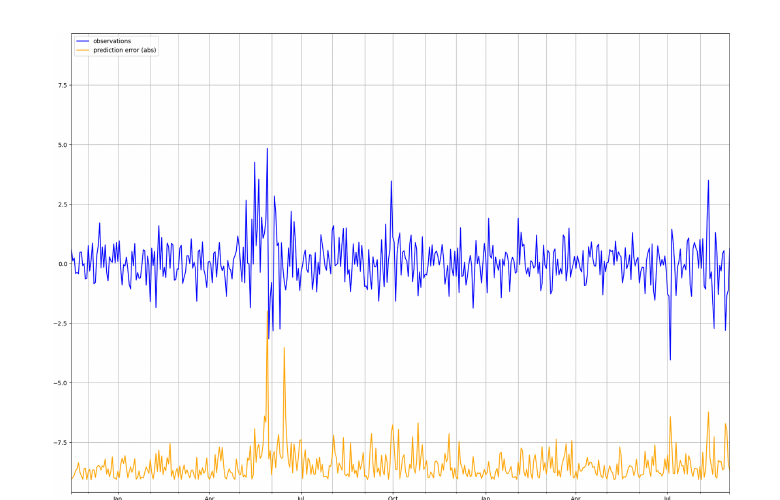
\includegraphics[width=0.85\linewidth]{gfx/m5l3_consoli_fig5.png}
\par\smallskip{\small \textbf{Hình 5.} Sai số dự báo tuyệt đối (MAFE) (màu cam) so với quan sát thực (màu xanh). (Nguồn: Consoli và cộng sự (2021), Hình 5)}
\end{figure}


Hiệu suất của mô hình giảm nhẹ từ cuối tháng 5 đến tháng 7/2018, tương ứng với giai đoạn bất ổn chính trị tại Ý. Thật vậy, ngày 29/5, chênh lệch lợi suất của Ý tăng mạnh, lên tới 250 điểm cơ bản. Nhà đầu tư đặc biệt lo ngại khả năng hình thành chính phủ chống đồng euro và thiếu niềm tin vào việc lập được một chính phủ ổn định. Từ tháng 6 đến tháng 11/2018, hàng loạt tranh luận về các cam kết chi tiêu thâm hụt và khả năng xung đột với các quy tắc tài khóa châu Âu tiếp tục khiến thị trường lo lắng. Chênh lệch lợi suất tăng mạnh vào tháng 10 và 11 với mức khoảng 300 điểm cơ bản. Điều này cũng thể hiện qua hiệu suất của mô hình, vốn giảm đôi chút trong giai đoạn căng thẳng này, nhưng nhìn chung mô hình vẫn xử lý khá tốt. Từ năm 2019, tình hình chính trị Ý bắt đầu cải thiện và chênh lệch lợi suất giảm dần, nhất là sau thỏa thuận với Brussels về thâm hụt ngân sách vào tháng 12/2018. Tuy nhiên, sau đó một số sự kiện đã tác động đến kinh tế Ý, như triển vọng tiêu cực của EU và cuộc bầu cử Nghị viện châu Âu, góp phần làm lãi suất tăng tạm thời. Trong giai đoạn này mô hình hoạt động khá tốt xét theo các tỷ lệ sai số tuyệt đối, cho thấy độ vững (robustness) tốt.

Hình 6 là biểu đồ phân tán giữa các điểm dự báo trung vị ngoài mẫu và các quan sát thực. Ở mức độ nào đó, các điểm trên biểu đồ bám khá sát đường chéo, cho thấy tương quan tốt giữa giá trị dự báo và quan sát thực, hàm ý chất lượng dự báo tốt. Điều này cũng được xác nhận bởi giá trị R-squared chấp nhận được là 0,23 trên các dự báo trung vị ngoài mẫu, đối với một bài toán dự báo nhiều thách thức như vậy. Giá trị R-squared này cho thấy mô hình LSTM giải thích được khá nhiều biến thiên của dữ liệu phản hồi quanh trung vị, gợi ý mức độ gần nhau nhất định giữa dữ liệu dự báo và quan sát thực.

\begin{figure}[H]
\centering
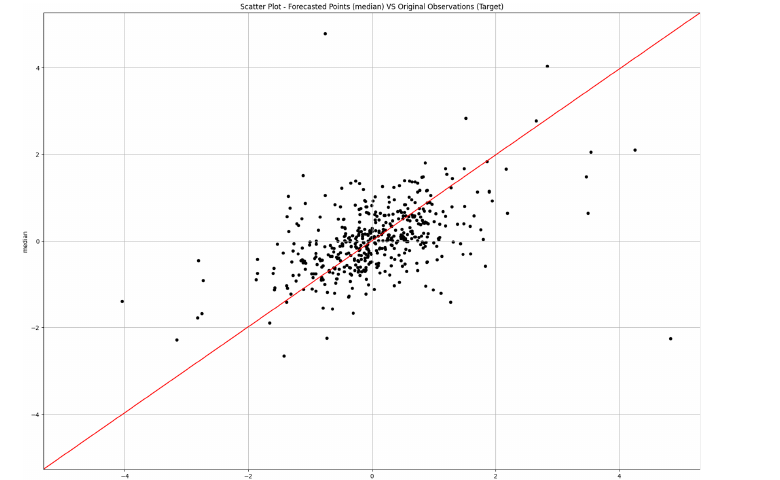
\includegraphics[width=0.85\linewidth]{gfx/m5l3_consoli_fig6.png}
\par\smallskip{\small \textbf{Hình 6.} Biểu đồ phân tán giữa các điểm dự báo trung vị ngoài mẫu và các quan sát thực. (Nguồn: Consoli và cộng sự (2021), Hình 6)}
\end{figure}


\section{6. Kết luận và triển vọng}

Bài báo trình bày công việc đang thực hiện về phương pháp xây dựng các chỉ báo kinh tế và tài chính thay thế, nắm bắt cảm xúc của nhà đầu tư và mức độ phổ biến của các chủ đề từ GDELT (Global Data on Events, Location, and Tone), một cơ sở dữ liệu nền tảng mở miễn phí chứa tin tức phát thanh, báo in và web toàn cầu theo thời gian thực. Dự án đang triển khai nhằm tạo ra các phương pháp dự báo cải tiến để phân tích thị trường trái phiếu chính phủ của các nước EU. Chúng tôi đã báo cáo một số kết quả sơ bộ khi áp dụng phương pháp này để dự báo thị trường trái phiếu chính phủ Ý. Trường hợp này cho thấy hiệu suất ban đầu tốt, gợi ý tính hợp lệ của cách tiếp cận. Nhờ sử dụng thông tin trích xuất từ truyền thông tin tức Ý trong GDELT kết hợp với mạng học sâu Long Short-Term Memory được huấn luyện và kiểm định phù hợp theo phương pháp cửa sổ trượt (rolling window), chúng tôi đã thu được kết quả dự báo khá tốt.

Đây là một trong những công trình đầu tiên nghiên cứu hành vi của chênh lệch lợi suất trái phiếu chính phủ và các quyết định danh mục đầu tư tài chính khi có mặt các nhân tố đường cong lợi suất cổ điển và thông tin trích xuất từ tin tức. Chúng tôi tin rằng các thước đo mới này có thể nắm bắt và dự báo các thay đổi trong động lực lãi suất, đặc biệt trong giai đoạn bất ổn. Nhìn chung, bài báo cho thấy cách dùng một cơ sở dữ liệu quy mô lớn như GDELT để xây dựng các chỉ báo tài chính nhằm nắm bắt ý định tương lai của các tác nhân trên thị trường trái phiếu chính phủ.

Chắc chắn cần nghiên cứu thêm theo các hướng đã nêu. Trước hết, chúng tôi sẽ cố gắng cải thiện hiệu suất của mô hình DeepAR đã triển khai bằng cách tinh chỉnh kiến trúc và tối ưu siêu tham số của mô hình LSTM. Ngoài ra, trong nghiên cứu hiện tại chúng tôi đang thử nghiệm các mô hình dự báo khác, từ phương pháp kinh tế truyền thống đến các phương pháp học máy mới, gồm Gradient Boosting Machines và các phương pháp dự báo bằng mạng nơ-ron. Trong phiên bản mở rộng sau này, chúng tôi sẽ so sánh và phân tích kỹ hiệu suất các phương pháp này để khai thác tốt hơn các tác động phi tuyến của các biến phụ thuộc. Khả năng diễn giải của các mô hình học máy, chẳng hạn bằng giá trị Shapley, sẽ là đối tượng nghiên cứu quan trọng trong tương lai nhằm đánh giá chính xác đóng góp của các biến đồng hành khác nhau vào dự báo của mô hình.

\textbf{Lời cảm ơn.} Các tác giả cảm ơn các đồng nghiệp tại Centre for Advanced Studies thuộc Joint Research Centre của Ủy ban châu Âu vì sự hướng dẫn và hỗ trợ hữu ích trong quá trình thực hiện nghiên cứu này.

\subsection{Tài liệu tham khảo}

\begin{enumerate}
\def\labelenumi{\arabic{enumi}.}
\item
  Agrawal, S., Azar, P., Lo, A.W., Singh, T.: Momentum, mean-reversion and social media: evidence from StockTwits and Twitter. J. Portfolio Manag. 44, 85--95
\end{enumerate}

\begin{enumerate}
\def\labelenumi{(\arabic{enumi})}
\setcounter{enumi}{2017}
\item
\end{enumerate}

\begin{enumerate}
\def\labelenumi{\arabic{enumi}.}
\setcounter{enumi}{1}
\item
  Alexandrov, A., et al.: GluonTS: probabilistic time series models in Python. CoRR, abs/1906.05264 (2019). http://arxiv.org/abs/1906.05264
\item
  Beber, A., Brandt, M.W., Kavajecz, K.A.: Flight-to-quality or flight-to-liquidity? Evidence from the Euro-area bond market. Rev. Financ. Stud. 22(3), 925--957
\end{enumerate}

\begin{enumerate}
\def\labelenumi{(\arabic{enumi})}
\setcounter{enumi}{2008}
\item
\end{enumerate}

\begin{enumerate}
\def\labelenumi{\arabic{enumi}.}
\setcounter{enumi}{3}
\item
  Benidis, K., et al.: Neural forecasting: introduction and literature overview. CoRR,
\end{enumerate}

abs/2004.10240 (2020). https://arxiv.org/abs/2004.10240

\begin{enumerate}
\def\labelenumi{\arabic{enumi}.}
\setcounter{enumi}{4}
\item
  Bernal, O., Gnabo, J.-Y., Guilmin, G.: Economic policy uncertainty and risk spillover in the Eurozone. J. Int. Money Finance 65(C), 24--45 (2016)
\item
  Borovykh, A., Bohte, S., Oosterlee, C.W.: Conditional time series forecasting with convolutional neural networks. Lecture Notes in Computer Science (including subseries Lecture Notes in Artificial Intelligence and Lecture Notes in Bioinformatics), vol. 10614, pp. 729--730 (2017)
\item
  Chang, Y.-C., Chang, K.-H., Wu, G.-J.: Application of eXtreme gradient boosting trees in the construction of credit risk assessment models for financial institutions. Appl. Soft Comput. J. 73, 914--920 (2018)
\item
  Deng, S., Wang, C., Wang, M., Sun, Z.: A gradient boosting decision tree approach for insider trading identification: an empirical model evaluation of china stock market. Appl. Soft Comput. J. 83 (2019)
\item
  Dridi, A., Atzeni, M., Reforgiato Recupero, D.: FineNews: fine-grained semantic sentiment analysis on financial microblogs and news. Int. J. Mach. Learn. Cybern., 1--9 (2018)
\item
  Favero, C., Pagano, M., von Thadden, E.-L.: How does liquidity affect government bond yields? J. Financ. Quant. Anal. 45(1), 107--134 (2010)
\item
  Garcia, A.J., Gimeno, R.: Flight-to-liquidity flows in the Euro area sovereign debt crisis. Technical report, Banco de Espana Working Papers (2014)
\item
  Gentzkow, M., Kelly, B., Taddy, M.: Text as data. J. Econ. Lit. (2019, to appear)
\item
  Gormley, C., Tong, Z.: Elasticsearch: The Definitive Guide. O' Reilly Media, Sebastopol (2015)
\item
  Hansen, S., McMahon, M.: Shocking language: understanding the macroeconomic effects of central bank communication. J. Int. Econ. 99, S114--S133 (2016)
\item
  Hochreiter, S., Schmidhuber, J.: Long short-term memory. Neural Comput. 9, 1735--1780 (1997)
\item
  Koenecke, A., Gajewar, A.: Curriculum learning in deep neural networks for financial forecasting. In: Bitetta, V., Bordino, I., Ferretti, A., Gullo, F., Pascolutti, S., Ponti, G. (eds.) MIDAS 2019. LNCS (LNAI), vol. 11985, pp. 16--31. Springer, Cham (2020). https://doi.org/10.1007/978-3-030-37720-5 2
\item
  Leetaru, K., Schrodt, P.A.: GDELT: global data on events, location and tone, 1979--2012. Technical report, KOF Working Papers (2013)
\item
  Liu, J., Wu, C., Li, Y.: Improving financial distress prediction using financial network-based information and GA-based gradient boosting method. Comput. Econ. 53(2), 851--872 (2019). https://doi.org/10.1007/s10614-017-9768-3
\item
  Loughran, T., McDonald, B.: When is a liability not a liability? Textual analysis, dictionaries and 10-ks. J. Finance 66(1), 35--65 (2011)
\item
  Manganelli, S., Wolswijk, G.: What drives spreads in the Euro area government bond markets? Econ. Policy 24(58), 191--240 (2009)
\item
  Mehdiyev, N., Enke, D., Fettke, P., Loos, P.: Evaluating forecasting methods by considering different accuracy measures. Procedia Comput. Sci. 95, 264--271 (2016)
\item
  Monfort, A., Renne, J.-P.: Decomposing Euro-area sovereign spreads: credit and liquidity risks. Rev. Finance 18(6), 2103--2151 (2013)
\item
  Nelson, C., Siegel, A.F.: Parsimonious modeling of yield curves. J. Bus. 60(4), 473--489 (1987)
\item
  Shah, N., Willick, D., Mago, V.: A framework for social media data analytics using Elasticsearch and Kibana. Wireless Networks (2018, in press)
\item
  Shapiro, A.H., Sudhof, M., Wilson, D.: Measuring news sentiment. Federal Reserve Bank of San Francisco Working Paper (2018)
\item
  Tetlock, P.C.: Giving content to investor sentiment: the role of media in the stock market. J. Finance 62(3), 1139--1168 (2007)
\item
  Thorsrud, L.A.: Nowcasting using news topics. big data versus big bank. Norges Bank Working Paper (2016)
\item
  Thorsrud, L.A.: Words are the new numbers: a newsy coincident index of the business cycle. J. Bus. Econ. Stat., 1--17 (2018)
\item
  Yang, X., He, J., Lin, H., Zhang, Y.: Boosting exponential gradient strategy for online portfolio selection: an aggregating experts' advice method. Comput. Econ. 55(1), 231--251 (2020). https://doi.org/10.1007/s10614-019-09890-2
\item
  Zhang, D., Hu, M., Ji, Q.: Financial markets under the global pandemic of COVID19. Finance Res. Lett., 101528 (2020)
\end{enumerate}

Giấy phép truy cập mở: Chương này được cấp phép theo Giấy phép Quốc tế Creative Commons Attribution 4.0 (http://creativecommons.org/licenses/by/4.0/), cho phép sử dụng, chia sẻ, phóng tác, phân phối và sao chép dưới mọi phương tiện hay định dạng, miễn là ghi nhận đúng tác giả gốc và nguồn, cung cấp liên kết tới giấy phép Creative Commons và nêu rõ các thay đổi (nếu có).

Hình ảnh hoặc tư liệu của bên thứ ba trong chương này thuộc giấy phép Creative Commons của chương, trừ khi có ghi chú khác trong phần ghi nguồn. Nếu tư liệu không thuộc giấy phép của chương và mục đích sử dụng của bạn không được quy định pháp luật cho phép hoặc vượt quá phạm vi cho phép, bạn cần xin phép trực tiếp chủ sở hữu bản quyền.

\chapter{Đọc thêm 3: Bộ dữ liệu GDELT và thị trường trái phiếu chính phủ Ý (Consoli và cộng sự)}
\label{ch:M5L3DocThem3}

\section{Thông tin nguồn}

\begin{itemize}
  \item \textbf{Nguồn:} Consoli, S., Tiozzo Pezzoli, L. \& Tosetti, E. ``Using the GDELT Dataset to Analyse the Italian Sovereign Bond Market.'' Springer, 2020.
  \item \textbf{Phần cần đọc:} tr. 190--202
  \item \textbf{Ghi chú:} bản chuyển ngữ tiếng Việt súc tích, bám cấu trúc nguồn (giữ nguyên tiêu đề, công thức, số liệu, bảng, chú thích và danh mục tài liệu tham khảo).
\end{itemize}

Sergio Consoli, Luca Tiozzo Pezzoli và Elisa Tosetti European Commission, Joint Research Centre, Directorate A-Strategy, Work Programme and Resources, Scientific Development Unit, Via E. Fermi 2749, 21027 Ispra, VA, Italy sergio.consoli@ec.europa.eu

\textbf{Tóm tắt.} GDELT (Global Data on Events, Location, and Tone) là cơ sở dữ liệu quy mô lớn, thời gian thực về xã hội loài người toàn cầu, phục vụ nghiên cứu mở; nó theo dõi tin tức phát thanh, báo in và báo mạng trên thế giới, tạo thành một nền tảng mở miễn phí để tính toán trên toàn bộ truyền thông thế giới. Trước hết, nhóm tác giả mô tả một trình thu thập dữ liệu (crawler) lấy siêu dữ liệu của GDELT theo thời gian thực và lưu vào hệ thống quản lý dữ liệu lớn dựa trên Elasticsearch, một công cụ tìm kiếm phổ biến và hiệu quả dựa trên thư viện Lucene. Sau đó, bằng cách khai thác và xử lý thông tin chi tiết của từng bản tin được mã hóa trong GDELT, nhóm xây dựng các chỉ báo phản ánh cảm xúc của nhà đầu tư, hữu ích cho việc phân tích thị trường trái phiếu chính phủ Ý. Dùng phân tích hồi quy và mô hình Gradient Boosting của học máy, nhóm nhận thấy các đặc trưng trích xuất từ GDELT cải thiện dự báo chênh lệch lợi suất trái phiếu chính phủ so với hồi quy cơ sở chỉ gồm các biến hồi quy truyền thống. Mức cải thiện về độ khớp đặc biệt rõ trong giai đoạn khủng hoảng chính phủ từ tháng 5 đến tháng 12/2018.

\textbf{Từ khóa:} chênh lệch lợi suất trái phiếu chính phủ · học máy · quản lý dữ liệu lớn · hồi quy phân vị · xây dựng đặc trưng (feature engineering) · GDELT

\section{1. Giới thiệu}

Sự bùng nổ của công nghệ tính toán và thông tin trong thập kỷ qua đã tạo ra lượng dữ liệu khổng lồ ở nhiều lĩnh vực, gọi là dữ liệu lớn (Big Data). Trong kinh tế và tài chính, việc khai thác các dữ liệu này đưa nghiên cứu và thực tiễn kinh doanh lại gần nhau, vì dữ liệu sinh ra từ hoạt động kinh tế thường ngày có thể dùng cho các hệ thống kinh tế học nhanh, liên tục cải thiện và cá nhân hóa mô hình. Việc ứng dụng công nghệ khoa học dữ liệu vào kinh tế và tài chính mang lại lợi ích cho cả nhà khoa học lẫn người làm nghề, cải thiện dự báo và dự báo tức thời (nowcasting) trong nhiều loại ứng dụng.

Cụ thể, đợt tăng mạnh gần đây của chênh lệch lợi suất trái phiếu chính phủ ở các nước khu vực đồng Euro đã làm dấy lên tranh luận sôi nổi về các yếu tố quyết định và nguồn rủi ro của chênh lệch lợi suất trái phiếu chính phủ. Theo truyền thống, các yếu tố như mức độ tín nhiệm, rủi ro thanh khoản của trái phiếu chính phủ và mức ngại rủi ro toàn cầu được xem là nhân tố chính tác động đến chênh lệch lợi suất {[}2,20{]}. Tuy nhiên, văn liệu gần đây chỉ ra vai trò quan trọng của cảm xúc nhà đầu tư tài chính trong việc dự đoán diễn biến lãi suất {[}17,25{]}.

Bài báo khai thác một cơ sở dữ liệu tin tức mã nguồn mở mới là Global Database of Events, Language and Tone (GDELT)¹ {[}15{]} để xây dựng các chỉ báo tài chính dựa trên tin tức, liên quan đến các sự kiện kinh tế và chính trị của một nhóm nước khu vực đồng Euro. Như mô tả ở Mục 3.1, do quy mô của GDELT khiến việc dùng cơ sở dữ liệu quan hệ để phân tích trong thời gian hợp lý là không khả thi, Mục 4.1 trình bày hạ tầng quản lý dữ liệu lớn dùng để lưu trữ và tương tác với dữ liệu. Sau khi dữ liệu GDELT được thu thập từ Web bằng các REST API² tùy biến, nhóm biến đổi và lưu chúng một cách hiệu quả vào hệ thống quản lý dữ liệu lớn dựa trên Elasticsearch, một công cụ tìm kiếm NoSQL phổ biến và hiệu quả (Mục 4.1).

Tiếp theo, quy trình xây dựng đặc trưng được áp dụng lên thông tin chi tiết mã hóa trong GDELT (Mục 4.2) nhằm chọn các biến hữu ích nhất, phản ánh, trong số khác, cảm xúc của nhà đầu tư và mức độ phổ biến của các chủ đề tin tức, phục vụ phân tích thị trường trái phiếu chính phủ Ý. Mục 4.3 mô tả mô hình Gradient Boosting được dùng để phân tích thị trường này. Phân tích thực nghiệm ở Mục 4.4 cho thấy mô hình học máy sử dụng các chỉ báo GDELT đã xây dựng có ích trong dự báo chênh lệch lợi suất trái phiếu chính phủ và bất ổn tài chính, phù hợp với các nghiên cứu trước.

\section{2. Các nghiên cứu liên quan}

Các bài báo tin tức là nguồn thông tin mới được bổ sung vào dữ liệu chuẩn dùng để mô hình hóa các biến kinh tế và tài chính. Một nghiên cứu sớm là {[}25{]}, dùng cảm xúc từ một chuyên mục của Wall Street Journal để chỉ ra rằng mức bi quan cao là yếu tố dự báo đáng kể cho sự hội tụ của giá cổ phiếu về giá trị cơ bản. Tiếp sau đó, nhiều bài báo khác tìm hiểu vai trò của tin tức trong dự báo, chẳng hạn các thông báo của doanh nghiệp, lợi suất cổ phiếu và biến động. Ví dụ, trong tài chính có các công trình gần đây áp dụng phân tích cảm xúc ngữ nghĩa từ mạng xã hội, vi blog tài chính và tin tức để cải thiện dự đoán thị trường chứng khoán (ví dụ {[}1,7{]}). Tuy nhiên, các cách tiếp cận này thường bị hạn chế do phạm vi nguồn tài chính lịch sử sẵn có hẹp. Gần đây tin tức cũng được dùng trong kinh tế vĩ mô. Chẳng hạn, {[}13{]} xem xét nội dung thông tin trong các tuyên bố của Cục Dự trữ Liên bang Mỹ và định hướng mà chúng cung cấp về diễn biến chính sách tiền tệ trong tương lai. Các bài báo khác ({[}26,27{]} và {[}23{]}, trong số

¹ Trang web GDELT: https://blog.gdeltproject.org/. ² Xem https://blog.gdeltproject.org/gdelt-2-0-our-global-world-in-realtime/.

(tiếp theo) ... và {[}23{]}, trong số những nghiên cứu khác, sử dụng phân bổ Dirichlet tiềm ẩn (Latent Dirichlet allocation, LDA) để phân loại bài báo theo chủ đề và tính các thước đo cảm xúc đơn giản dựa trên phân loại chủ đề đó. Mục tiêu là trích xuất tín hiệu có thể có giá trị dự báo đối với các thước đo hoạt động kinh tế như GDP, thất nghiệp và lạm phát {[}11{]}. Kết quả cho thấy cảm xúc kinh tế là bổ sung hữu ích cho các biến dự báo thường dùng để theo dõi và dự báo chu kỳ kinh doanh {[}7{]}.

Các phương pháp học máy trong tài liệu hiện có nhằm kiểm soát các chỉ số tài chính đo lường rủi ro tín dụng, rủi ro thanh khoản và mức ngại rủi ro gồm các công trình {[}2,4,8,9,18{]}, cùng nhiều công trình khác. Nỗ lực đưa các mô hình học máy vào lĩnh vực mô hình hóa kinh tế đã tăng nhanh theo cấp số nhân trong những năm gần đây {[}19,24{]}. Trong các phương pháp học máy phổ biến, Gradient Boosting machines đã tỏ ra thành công trong nhiều bài toán dự báo thuộc kinh tế và tài chính (xem {[}5,6,16,28{]}, cùng nhiều công trình khác).

\section{3. Dữ liệu}

\subsection{3.1. Về GDELT}

GDELT là cơ sở dữ liệu toàn cầu về sự kiện, địa điểm và sắc thái do Google duy trì {[}15{]}. Đây là nền tảng Dữ liệu lớn (Big Data) mở về tin tức thu thập trên toàn thế giới, chứa dữ liệu có cấu trúc khai thác từ nguồn tin truyền hình, báo in và web bằng hơn 65 ngôn ngữ. GDELT liên kết con người, tổ chức, trích dẫn, địa điểm, chủ đề và cảm xúc gắn với các sự kiện trên thế giới; mô tả hành vi xã hội qua lăng kính truyền thông, nên là nguồn dữ liệu lý tưởng để đo các yếu tố xã hội và kiểm định giả thuyết. Về quy mô, GDELT phân tích hơn 88 triệu bài báo mỗi năm từ hơn 150.000 cơ quan báo chí; dung lượng khoảng 8 TB, tăng thêm 2 TB mỗi năm. GDELT gồm hai bộ dữ liệu chính: "Global Knowledge Graph (GKG)" và "Events Table"; nghiên cứu này dùng bộ thứ nhất. GKG ghi nhận điều đang diễn ra trên thế giới, bối cảnh, những ai liên quan và thế giới cảm nhận ra sao, mỗi ngày; đồng thời cung cấp bản dịch tiếng Anh của thông tin đã mã hóa từ các ngôn ngữ được hỗ trợ. Ngoài ra, các chủ đề được ánh xạ sang các hệ phân loại chủ đề thông dụng trong thực tiễn, như "World Bank (WB) Topical Ontology" (3), hoặc hệ phân loại chủ đề tích hợp của GDELT. GDELT cũng đo hàng nghìn chiều cảm xúc dựa trên các từ điển phổ biến như "Harvard IV-4 Psychosocial Dictionary" (4), "WordNet-Affect dictionary" (5) và "Loughran and McDonald Sentiment Word Lists dictionary" (6), cùng các từ điển khác. Trong ứng dụng này, chúng tôi dùng các trường GKG của GDELT gồm World Bank Topical Ontology (tức các chủ đề WB), toàn bộ chiều cảm xúc (GCAM) và tên cơ quan báo chí.

Chú thích:

\begin{itemize}
\item
  \begin{enumerate}
  \def\labelenumi{(\arabic{enumi})}
  \setcounter{enumi}{2}
    \item
    https://vocabulary.worldbank.org/taxonomy.html
  \end{enumerate}
\item
  \begin{enumerate}
  \def\labelenumi{(\arabic{enumi})}
  \setcounter{enumi}{3}
    \item
    http://www.wjh.harvard.edu/\textasciitilde inquirer/homecat.htm
  \end{enumerate}
\item
  \begin{enumerate}
  \def\labelenumi{(\arabic{enumi})}
  \setcounter{enumi}{4}
    \item
    http://wndomains.fbk.eu/wnaffect.html
  \end{enumerate}
\item
  \begin{enumerate}
  \def\labelenumi{(\arabic{enumi})}
  \setcounter{enumi}{5}
    \item
    https://sraf.nd.edu/textualanalysis/resources/
  \end{enumerate}
\end{itemize}

\subsection{3.2. Chênh lệch lợi suất}

Chúng tôi trích dữ liệu từ Bloomberg về cấu trúc kỳ hạn của lợi suất trái phiếu chính phủ Ý trong giai đoạn 2/3/2015 đến 31/8/2019. Chênh lệch lợi suất trái phiếu chính phủ (sovereign spread) của Ý so với Đức được tính bằng lợi suất trái phiếu kỳ hạn 10 năm của Ý trừ lợi suất tương ứng của Đức. Chúng tôi cũng trích các nhân tố chuẩn về mức (level), độ dốc (slope) và độ cong (curvature) của cấu trúc kỳ hạn bằng phương pháp Nelson và Siegel {[}21{]}.

Chúng tôi ước lượng mô hình dự báo chênh lệch tín dụng dùng các nhân tố đường cong lợi suất thông thường cùng các đặc trưng GDELT được chọn, và so sánh với mô hình dự báo cổ điển chỉ dùng mức, độ dốc và độ cong làm biến hồi quy.

\section{4. Phương pháp}

\subsection{4.1. Quản lý Dữ liệu lớn}

Các bộ dữ liệu phi cấu trúc khổng lồ như GDELT cần được lưu trong hệ thống tệp phân tán (DFS) chuyên dụng, kết nối nhiều nút tính toán qua mạng, vốn thiết yếu để xây dựng các đường ống dữ liệu phân lớp và tổng hợp lượng thông tin lớn này. Trong các nền tảng DFS phổ biến, do lượng tài liệu phi cấu trúc khổng lồ từ GDELT, chúng tôi dùng Elasticsearch {[}12,22{]} để lưu trữ và tương tác với dữ liệu. Elasticsearch là kho tài liệu phổ biến và hiệu quả; thay vì lưu thông tin thành các hàng dữ liệu dạng cột như cơ sở dữ liệu quan hệ cổ điển, nó lưu các cấu trúc dữ liệu phức tạp được tuần tự hóa thành tài liệu JSON. Được xây dựng trên thư viện tìm kiếm Apache Lucene (7), nó cung cấp tìm kiếm và phân tích thời gian thực cho nhiều loại dữ liệu có cấu trúc hoặc phi cấu trúc.

Elasticsearch có kiến trúc phân tán, cho phép nối nhiều nút Elasticsearch thành một cụm duy nhất. Ngay khi tài liệu được lưu, nó được lập chỉ mục và có thể tìm kiếm đầy đủ gần như theo thời gian thực. Một chỉ mục (index) Elasticsearch có thể xem là tập hợp tài liệu được tối ưu hóa, mỗi tài liệu là tập hợp các trường (field), tức các cặp khóa-giá trị chứa dữ liệu. Chỉ mục thực chất chỉ là nhóm logic gồm một hoặc nhiều phân mảnh (shard) vật lý, mỗi phân mảnh là một chỉ mục tự chứa.

Elasticsearch cũng không cần lược đồ (schema-less): tài liệu có thể được lập chỉ mục mà không cần chỉ định rõ cách xử lý từng trường có thể xuất hiện. Elasticsearch cung cấp REST API đơn giản để quản lý cụm và tương tác với tài liệu đã lưu; có thể gửi yêu cầu API trực tiếp từ dòng lệnh hoặc qua Developer Console trong giao diện web người dùng, gọi là Kibana (8). Các REST API của Elasticsearch hỗ trợ truy vấn có cấu trúc, truy vấn toàn văn và truy vấn phức hợp kết hợp cả hai, dùng ngôn ngữ truy vấn kiểu JSON của Elasticsearch, gọi là Query DSL (9).

Chú thích:

\begin{itemize}
\item
  \begin{enumerate}
  \def\labelenumi{(\arabic{enumi})}
  \setcounter{enumi}{6}
    \item
    https://lucene.apache.org/
  \end{enumerate}
\item
  \begin{enumerate}
  \def\labelenumi{(\arabic{enumi})}
  \setcounter{enumi}{7}
    \item
    Kibana, phiên bản 7.4: https://www.elastic.co/guide/en/kibana/7.4/
  \end{enumerate}
\end{itemize}

Kỹ thuật đặc trưng (Feature Engineering)

GDELT bổ sung bài báo mới mỗi mười lăm phút, mỗi bài được biểu diễn gọn thành một hàng của bảng GDELT ở định dạng .csv. Bảng GKG chứa khoảng 10 TB dữ liệu, cần được tích hợp và nạp dưới dạng các tài liệu JSON tuần tự hóa vào khung Elasticsearch. Việc này gồm ba bước ETL thông thường (Extract, Transform, Load), phải nhận diện và khắc phục sự không đồng nhất về cấu trúc, cú pháp và ngữ nghĩa của dữ liệu. Vì vậy nhóm tác giả dùng World Bank Topical Ontology để xác định trọng tâm (chủ đề) của từng bài báo và chọn những tin có chủ đề chính liên quan đến các sự kiện mà nhà đầu tư thị trường trái phiếu quan tâm. Bảng phân loại này là lược đồ mô tả các lĩnh vực chuyên môn và tri thức của Ngân hàng Thế giới, phản ánh ngôn ngữ của các chuyên gia trong từng lĩnh vực. GDELT ghi toàn bộ các chủ đề được thảo luận trong một bài báo vào một hàng duy nhất; nhóm tách các chủ đề này thành những mục riêng.

Nhóm trích xuất tin tức từ GKG của khoảng 20 tờ báo Ý, xuất bản từ tháng 3/2015 đến cuối tháng 8/2019. Nhóm dựa vào tệp Geographic Source Lookup trên blog GDELT\^{}10 để chọn cả các báo quốc gia tổng hợp có lượng phát hành lớn nhất lẫn các báo chuyên về tài chính và kinh tế. Sau khi thu thập, tin được ánh xạ vào ngày giao dịch tương ứng: các bài đăng trong giờ mở cửa thị trường trái phiếu (9h00-17h30) được gán cho ngày giao dịch đó; bài đăng sau giờ đóng cửa hoặc qua đêm được gán cho ngày giao dịch kế tiếp.\^{}11 Theo {[}10{]}, tin đăng vào cuối tuần được gán cho thứ Hai; bài đăng trong ngày lễ hoặc cuối tuần liền trước ngày lễ bị loại.

Tiếp theo, chỉ giữ các bài có chủ đề do GDELT trích xuất thuộc một trong các chủ đề WB quan tâm: Macroeconomic Vulnerability and Debt (Tính dễ tổn thương kinh tế vĩ mô và nợ) và Macroeconomic and Structural Policies (Chính sách kinh tế vĩ mô và cơ cấu). Có bài chỉ nhắc thoáng một chủ đề được chọn rồi chuyển sang chủ đề hoàn toàn khác. Để bảo đảm trọng tâm của bài là một chủ đề WB đã chọn, nhóm chỉ giữ tin có ít nhất ba từ khóa thuộc các chủ đề này trong nội dung, nhằm chọn tin tập trung vào các vấn đề liên quan đến thị trường trái phiếu và loại tin chỉ lướt qua các vấn đề kinh tế vĩ mô, nợ và chính sách cơ cấu. Cuối cùng, để tập tin không quá chênh lệch về độ dài, chỉ giữ các bài dài tối thiểu 100 từ. Sau quy trình chọn lọc này còn tổng cộng 18.986 bài báo.

Từ lượng thông tin này, nhóm xây dựng các đặc trưng bằng cách đếm tổng số từ thuộc mọi chủ đề WB và GCAM được phát hiện mỗi ngày. Nhóm cũng tạo biến "Number of mentions" (số lần được nhắc đến), là số từ của mỗi địa điểm xuất hiện trong các tin được chọn. Kết quả thu được 2.978 GCAM, 1.996 chủ đề và 155 địa điểm. Lưu ý mọi đặc trưng đều tính theo số từ mỗi ngày, trừ từ điển ANEW (v19) và thước đo hạnh phúc Hedonometer (v21) vốn đã là điểm số.

Sau khi trích xuất dữ liệu từ GKG, nhóm áp dụng quy trình năm bước để lọc các đặc trưng từ tin tức:

\begin{itemize}
\item
  Bước 1: dùng tiêu chí tri thức chuyên môn, giữ lại tập con gồm 413 từ điển GCAM có khả năng liên quan, cụ thể là 31 chiều của từ điển tâm lý xã hội General Inquirer Harvard IV, 61 chiều của Roget\textquotesingle s Thesaurus, 7 chiều của Martindale Regressive Imagery và 3 chiều của từ điển Affective Norms for English Words (ANEW).
\item
  Bước 2: xét mức biến thiên của đặc trưng; giữ các biến có độ lệch chuẩn trên toàn mẫu lớn hơn 5 từ và cho phép tối đa 10\% giá trị thiếu trên tổng số ngày. Ngoài ra loại các đặc trưng thiếu dữ liệu ở đầu mẫu (hơn 33\% mẫu).
\item
  Bước cuối: phân tích tương quan giữa các biến đã chọn. Trước hết chuẩn hóa mọi đặc trưng theo số bài báo mỗi ngày. Nếu tương quan giữa hai đặc trưng bất kỳ vượt 80\%, ưu tiên biến ít giá trị thiếu hơn; nếu số giá trị thiếu bằng nhau và hai biến cùng loại (cùng là chủ đề hoặc cùng là GCAM) thì chọn ngẫu nhiên một biến; nếu số giá trị thiếu bằng nhau nhưng khác loại thì theo thứ tự ưu tiên: GCAM, chủ đề WB, chủ đề GDELT, địa điểm.
\end{itemize}

Sau quy trình kỹ thuật đặc trưng này còn lại 45 biến: 9 chủ đề, 34 GCAM và 2 địa điểm. Xem xét các chủ đề được chọn cho thấy các chủ đề WB như Inflation (lạm phát), Government (chính phủ), Central Banks (ngân hàng trung ương), Taxation (thuế) và Policy (chính sách) đã được chọn; đây là những chủ đề quan trọng trong tin tức khi xét các vấn đề lãi suất. Ngoài ra, các đặc trưng xây dựng từ chiều GCAM như lạc quan, bi quan hoặc mức độ kích động (arousal) cũng được đưa vào, cho phép khảo sát trạng thái cảm xúc của thị trường.

Chú thích:

\begin{enumerate}
\def\labelenumi{\arabic{enumi}.}
\setcounter{enumi}{9}
\item
  https://blog.gdeltproject.org/mapping-the-media-a-geographic-lookup-pf-gdelts-sources/
\item
  Vì GKG dùng giờ UTC (https://blog.gdeltproject.org/new-gkg-20-article-metadata-fields/), nhóm đã hiệu chỉnh lệch một giờ theo múi giờ Ý.
\end{enumerate}

4.3 Phân tích dữ liệu lớn (Big Data Analytics)

Các mô hình kinh tế cổ điển không thể mở rộng linh hoạt để xử lý và duy trì các cấu trúc dữ liệu lớn (Big Data) như GDELT mà nghiên cứu này sử dụng. Cần có một bộ mô hình và công cụ phân tích dữ liệu lớn mới, vững chắc trong không gian nhiều chiều, như các phương pháp của học máy {[}19,24{]}. Cụ thể, trong nghiên cứu tính toán này, nhóm tác giả chọn Gradient Boosting (GB) {[}14{]}, một phương pháp học máy nổi tiếng đã chứng tỏ hiệu quả trong nhiều bài toán mô hình hóa thuộc kinh tế và tài chính {[}5,6,16,28{]}. Gradient boosting là kỹ thuật học máy cho các bài toán hồi quy và phân loại, tạo ra mô hình dự báo dưới dạng một tập hợp (ensemble) các mô hình dự báo yếu, thường là cây quyết định. Mô hình được xây dựng theo từng giai đoạn như các phương pháp boosting khác, và tổng quát hóa chúng bằng cách cho phép tối ưu hóa một hàm mất mát khả vi tùy ý. Nói cách khác, đây là thuật toán tối ưu một hàm chi phí trên không gian hàm bằng cách lặp lại việc chọn một hàm (giả thuyết yếu) theo hướng gradient âm.

Về triển khai, nghiên cứu dùng thư viện H2O {[}12{]} cho ngôn ngữ lập trình R. H2O là nền tảng học máy mã nguồn mở, có khả năng mở rộng, cung cấp các triển khai song song của nhiều thuật toán học máy có giám sát và không giám sát, trong đó có Gradient Boosting Machines.

Để xác định giá trị tối ưu cho các tham số của mô hình GB, nghiên cứu dùng kiểm định chéo 10 lần (10-fold cross-validation) kết hợp thủ tục tìm kiếm lưới (grid search, hay quét tham số) {[}3{]}. Tìm kiếm lưới là việc duyệt vét cạn một tập con do người dùng chỉ định của không gian siêu tham số của thuật toán học, được dẫn dắt bởi một thước đo hiệu năng (ở đây là cực tiểu hóa sai số bình phương trung bình). Hai tham số chính cần tối ưu trong mô hình GB là:

\begin{itemize}
\item
  độ sâu tối đa của cây, cho biết độ sâu lớn nhất có thể của một cây trong mô hình và dùng để kiểm soát quá khớp (over-fitting), vì độ sâu lớn hơn cho phép mô hình học những quan hệ rất đặc thù của một mẫu cụ thể;
\item
  tốc độ học (learning rate), xác định mức ảnh hưởng của mỗi cây lên kết quả cuối cùng của mô hình GB. GB bắt đầu từ một ước lượng ban đầu, được cập nhật bằng đầu ra của từng cây; tốc độ học điều khiển độ lớn của thay đổi này. Vì vậy, giá trị thấp thường được ưu tiên do giúp mô hình vững trước các đặc điểm riêng của từng cây và nhờ đó khái quát hóa tốt. Tuy nhiên, giá trị thấp đòi hỏi nhiều cây hơn để mô hình hóa mọi quan hệ và tốn kém về tính toán.
\end{itemize}

Để khám phá không gian siêu tham số nhằm tìm giá trị tối ưu, thủ tục tìm kiếm lưới kiểm thử mô hình GB với độ sâu tối đa của cây từ 1 đến 10 (bước 1) và tốc độ học từ 0,01 đến 0,99 (bước 0,10); các giá trị tham số tốt nhất theo sai số bình phương trung bình được xuất ra. Nếu một giá trị tham số đạt đến cận trên hoặc cận dưới của khoảng tìm kiếm (tức nghiệm biên, corner solution), một cách tiếp cận tham lam (greedy) được lặp lại: biên tìm kiếm của tham số đó được dịch chuyển, và tìm kiếm lưới được khởi động lại từ các tham số dưới tối ưu của lần ước lượng trước. Thủ tục dừng khi cả hai giá trị tham số nằm trong biên tìm kiếm tương ứng, và các giá trị này là kết quả đầu ra. Tuy tìm kiếm lưới không đảm bảo tuyệt đối sẽ tìm được giá trị tham số tối ưu toàn cục, thực tế nhóm tác giả thấy nó hoạt động khá tốt, dù tốn kém về tính toán. Nhìn chung, tìm kiếm lưới là thủ tục được áp dụng và chấp nhận rộng rãi cho loại tác vụ tinh chỉnh này {[}3{]}.

{[}12{]} Giao diện R cho nền tảng học máy mở rộng "H2O": https://cran.rproject.org/web/packages/h2o/index.html.

\subsection{4.4 Phân tích thực nghiệm}

Mục tiêu chính của thực nghiệm là đánh giá sức dự báo của các đặc trưng GDELT được chọn, bên cạnh các yếu tố quyết định cổ điển của chênh lệch lợi suất (credit spread) trái phiếu chính phủ trong các giai đoạn căng thẳng. Nhóm tác giả xét khả năng dự báo ở phân vị thứ 90 của phân phối credit spread, vì mức này thường được xem là tình trạng khủng hoảng tài chính (xem {[}4{]}). Nhiều nghiên cứu cho thấy trong các giai đoạn này, các quan hệ phi tuyến phức tạp giữa các biến giải thích tác động đến biến mục tiêu mà các mô hình tuyến tính đơn giản không nắm bắt được. Do đó nhóm dùng mô hình GB (Gradient Boosting) với phân phối phân vị và kỹ thuật ước lượng cửa sổ trượt, với mẫu ước lượng đầu tiên bắt đầu từ đầu tháng 3 đến tháng 5/2017. Hiệu quả dự báo của mô hình GB gồm cả các yếu tố cổ điển lẫn các đặc trưng GDELT được chọn được so sánh với mô hình GB chỉ gồm các yếu tố cổ điển. Hiệu quả dự báo được đo bằng sai số tuyệt đối của từng dự báo. Sức giải thích của các đặc trưng GDELT theo thời gian được đánh giá qua độ quan trọng của biến ở mỗi lần ước lượng, và xét năm biến quan trọng nhất ở mỗi cửa sổ trượt, phù hợp với văn liệu cấu trúc kỳ hạn chuẩn: ba đến năm nhân tố là đủ để giải thích động thái của chênh lệch lợi suất. Mô hình được ước lượng trên nửa mẫu và dùng cửa sổ trượt để tạo dự báo trước một bước. Mỗi cửa sổ ước lượng dùng kiểm định chéo 10 lớp (10-fold cross-validation) và thủ tục tìm kiếm lưới (grid search) mô tả ở Mục 4.3 để chọn siêu tham số tối ưu cho mô hình GB.

Hình 1 trình bày chuỗi thời gian của chênh lệch lợi suất Ý và tỷ số giữa sai số dự báo tuyệt đối của mô hình bổ sung đặc trưng GDELT với mô hình chỉ có các biến hồi quy cổ điển. Khi tỷ số này nhỏ hơn 1, mô hình bổ sung tốt hơn chuẩn so sánh (benchmark). Hiệu quả của mô hình bổ sung cải thiện đáng kể từ cuối tháng 5/2018, khi khủng hoảng chính trị bắt đầu ở Ý. Ngày 29/5, chênh lệch lợi suất của Ý tăng mạnh lên 250 điểm cơ bản; nhà đầu tư lo ngại về khả năng có chính phủ chống đồng euro và thiếu tin tưởng vào việc lập một chính phủ ổn định. Trong các sự kiện căng thẳng này, mô hình bổ sung đặc trưng GDELT vượt trội rõ rệt so với benchmark, với tỷ số tuyệt đối thấp hơn nhiều so với 1, thấp nhất là 0,93 vào ngày 24/5 (giá trị nhỏ nhất trong toàn mẫu). Kết quả này nhấn mạnh giá trị gia tăng của tin tức báo chí trong dự báo động thái chênh lệch lợi suất ở giai đoạn khủng hoảng tài chính. Từ tháng 6 đến tháng 11/2018, các tranh luận về cam kết chi tiêu thâm hụt và khả năng xung đột với quy tắc tài khóa châu Âu tiếp tục khiến thị trường lo ngại. Chênh lệch lợi suất tăng mạnh vào tháng 10 và tháng 11, quanh mức 300 điểm cơ bản.

\textbf{Hình 1.} Tỷ số sai số tuyệt đối và chênh lệch lợi suất

Trong giai đoạn này, mô hình bổ sung lại hoạt động đặc biệt tốt, tỷ số quanh 0,95, thấp nhất 0,94 vào ngày 9/11. Từ năm 2019, tình hình chính trị Ý cải thiện và chênh lệch lợi suất giảm êm, nhất là sau thỏa thuận với Brussels về thâm hụt ngân sách vào tháng 12/2018. Tuy nhiên, sau đó một số sự kiện tác động đến kinh tế Ý, như triển vọng tiêu cực của EU và bầu cử Nghị viện châu Âu, làm lãi suất tăng tạm thời. Dù năm 2019 mô hình bổ sung không tốt bằng năm 2018 xét theo tỷ số sai số tuyệt đối, nó vẫn luôn vượt benchmark. Từ phân tích trên có thể thấy ba giai đoạn con: giai đoạn trước khủng hoảng từ 7/2017 đến 5/2018; giai đoạn khủng hoảng từ tháng 6 đến tháng 12/2018; và giai đoạn từ tháng 1/2019 đến hết mẫu. Tiếp theo, đóng góp của từng đặc trưng GDELT được chọn trong dự báo chênh lệch lãi suất ở giai đoạn căng thẳng chính trị được phân tích theo ba giai đoạn con này.

Hình 2 cho thấy tần suất mỗi biến xuất hiện trong năm vị trí đầu theo độ quan trọng biến của Gradient Boosting Machine trong (a) giai đoạn trước khủng hoảng, (b) giai đoạn khủng hoảng và (c) giai đoạn sau khủng hoảng. Trong giai đoạn trước khủng hoảng, các yếu tố cổ điển như độ dốc và độ cong của đường cong chênh lệch lợi suất là các biến quan trọng nhất. Tuy nhiên, trong các biến hồi quy cổ điển, nhân tố mức (level), vốn được văn liệu xem là biến quan trọng nhất giải thích động thái lãi suất, lại kém quan trọng hơn hai thước đo cảm xúc GCAM, cụ thể là arousal từ từ điển ANEW và Hate từ Thesaurus. Hình 2(b) cho thấy trong giai đoạn khủng hoảng, đóng góp dự báo của các yếu tố chênh lệch lợi suất cổ điển giảm đáng kể. Biến quan trọng nhất là Arousal.

Hình 2. Mức độ quan trọng của biến: phần trăm số lần các biến nằm trong top 5 (các bảng: (a) giai đoạn trước khủng hoảng chính phủ; (b) giai đoạn khủng hoảng chính phủ; (c) giai đoạn sau khủng hoảng chính phủ).

Chỉ số của từ điển ANEW đứng đầu. Đáng chú ý, các đề cập đến địa danh Đức và "Government" (chính phủ) chiếm vị trí thứ hai và thứ ba. Nhân tố độ dốc (slope) kinh điển chỉ xếp thứ năm. Cuối cùng, Hình 2(c) cho thấy năm 2019, tầm quan trọng của nhân tố mức (level) tăng mạnh, cùng với các đề cập đến các vấn đề chính sách tiền tệ. ANEW Arousal và các đề cập đến chính phủ vẫn nằm trong danh sách top 5, nghĩa là các thảo luận mang nhiều cảm xúc về các vấn đề của chính phủ vẫn quan trọng trong giai đoạn hậu căng thẳng. Cần nhấn mạnh rằng, giống như giai đoạn hậu khủng hoảng, chỉ có một trong ba biến dự báo kinh điển nằm ngoài danh sách top 5.

\section{5 Kết luận}

Phân tích của chúng tôi là một trong những nghiên cứu đầu tiên về hành vi của chênh lệch lợi suất trái phiếu chính phủ và các quyết định danh mục đầu tư tài chính khi có mặt cả các nhân tố đường cong lợi suất kinh điển lẫn các thước đo cảm xúc tài chính trích xuất từ tin tức. Chúng tôi tin rằng các thước đo mới này có thể nắm bắt và dự báo những thay đổi trong động lực lãi suất, đặc biệt trong thời kỳ biến động mạnh. Thực nghiệm cho thấy đóng góp của các chiều cảm xúc là đáng kể trong những giai đoạn như vậy, thậm chí lớn hơn các nhân tố lãi suất kinh điển. Đáng chú ý, tầm quan trọng của các thước đo này còn kéo dài sang giai đoạn hậu khủng hoảng, nghĩa là các đặc trưng của chúng tôi nắm bắt được những câu chuyện giàu cảm xúc về các vấn đề chính phủ và chính sách tiền tệ vốn vẫn là tâm điểm của tin tức sau khủng hoảng. Nhìn chung, bài báo cho thấy cách dùng một cơ sở dữ liệu quy mô lớn như GDELT để rút ra các chỉ báo tài chính nhằm nắm bắt ý định tương lai của các tác nhân trên thị trường trái phiếu. Trong nghiên cứu tiếp theo, chúng tôi sẽ áp dụng thêm các kỹ thuật học máy để khai thác tốt hơn các hiệu ứng phi tuyến lên các biến phụ thuộc.

% ---- Lesson 4 ----
\chapter{TƯ DUY PHẢN BIỆN ĐỂ ĐÁNH GIÁ ĐỘ XÁC THỰC CỦA DỮ LIỆU}
\label{ch:M5L4LessonNotes}

\section*{Lesson Notes}

MODULE 5 \textbar{} LESSON 4

Thời gian đọc: 15 phút

Kiến thức nền: Toàn bộ nội dung Financial Data, nội dung Financial Markets Module 7

Từ khóa: Năng lực thông tin (Information Literacy), Tin giả (Fake News)

Trong bài học này, chúng ta xem xét các đặc điểm của tư duy phản biện (critical thinking). Chúng ta sẽ tìm hiểu một bài tổng quan tài liệu có hệ thống, trong đó đề cập đến việc các kỹ năng tư duy phản biện được sử dụng như thế nào để xác định một tin tức có phải là "tin giả" hay không.

\section{Tư duy phản biện}

Tư duy phản biện không chỉ là điều chúng ta bàn một lần rồi thôi. Như Ismail viết: "Tư duy phản biện bao gồm tư duy có chủ đích, hướng đến mục tiêu trong quá trình đưa ra quyết định dựa trên bằng chứng trong quá trình giải quyết vấn đề khoa học" (1). Trong suốt chương trình này, bạn sẽ được kỳ vọng vận dụng các kỹ năng tư duy phản biện cho nhiều mục đích khác nhau, nhưng ở đây, chúng ta sẽ tập trung vào việc dùng tư duy phản biện để xác định một nguồn tin có đáng tin cậy hay không.

Bài báo của Ismail đề cập tầm quan trọng của các kỹ năng tư duy phản biện đối với việc được tuyển dụng và làm việc hiệu quả sau khi đã có việc làm. Bài báo nêu bật một nghiên cứu được thực hiện trên những nhân viên có năm năm kinh nghiệm trong công việc kỹ thuật, đặc biệt là kỹ thuật cơ khí. Khoảng thời gian năm năm được xem là điểm khởi đầu để hình thành sự trưởng thành trong sự nghiệp của một người.

Theo nghiên cứu này, bảng câu hỏi sau đã được gửi cho các kỹ sư cơ khí có 5 năm kinh nghiệm làm việc. Các câu hỏi liên quan đến:

\begin{itemize}
\item
  Xác định vấn đề trong một hệ thống phức tạp
\item
  Cải thiện kỹ năng giải thích, phân tích và đánh giá
\item
  Tìm kiếm các giải pháp thay thế
\item
  Tìm kiếm các giải pháp sáng tạo
\item
  Biện minh cho các quyết định dựa trên bằng chứng vững chắc
\item
  Khả năng kiên trì hoàn thành các trách nhiệm được giao
\item
  Khả năng hiểu và thích nghi với văn hóa của cộng đồng
\end{itemize}

Các kỹ năng tư duy phản biện rất được ưa chuộng trong môi trường làm việc vì chúng cần thiết để làm việc hiệu quả trong nhóm, phân tích dữ liệu, xây dựng lập luận, ra quyết định và giải quyết vấn đề. Do đó, điều quan trọng là bạn nên củng cố kỹ năng này hết mức có thể trong suốt chương trình.

Kỹ năng tư duy phản biện của bạn sẽ được đánh giá theo nhiều cách khác nhau, từ các bài đăng trên diễn đàn, các dự án làm việc nhóm cho đến dự án tốt nghiệp (capstone). Một kỹ năng tư duy phản biện mà chúng ta tập trung ở đây là năng lực thông tin (information literacy), vốn rất cần thiết khi bạn tìm kiếm các nguồn hợp lệ và đáng tin cậy để tìm dữ liệu cần dùng, để củng cố và phát triển ý tưởng của mình, v.v. Những kỹ năng này vô cùng quan trọng trong các công việc kỹ thuật tài chính cũng như các ngành nghề liên quan đến STEM khác. Ở phần sau của bài học này, chúng ta sẽ vận dụng kỹ năng tư duy phản biện để xác định một tin tức là tin giả hay đáng tin cậy.

\begin{enumerate}
\def\labelenumi{\arabic{enumi}.}
\setcounter{enumi}{1}
\item
  Năng lực thông tin
\end{enumerate}

Hiệp hội Thư viện Hoa Kỳ (American Library Association) định nghĩa năng lực thông tin là "một tập hợp các khả năng đòi hỏi mỗi cá nhân phải nhận biết khi nào cần thông tin và có khả năng tìm kiếm, đánh giá và sử dụng hiệu quả thông tin cần thiết." Như vậy, năng lực thông tin nghĩa là trước hết bạn biết cách nghiên cứu và tìm các nguồn mình cần, đồng thời biết cách đánh giá xem một nguồn có phải là nguồn thông tin đáng tin cậy và xác thực hay không. Tuy nghe có vẻ đơn giản, nhưng đây đã trở thành một nhiệm vụ ngày càng khó khăn khi tin giả, thông tin do cộng đồng đóng góp (crowdsourced) và các tác giả ẩn danh trên internet xuất hiện.

Vì vậy, việc đầu tiên chúng tôi yêu cầu bạn làm là hoàn thành hai mô-đun trong hướng dẫn Năng lực thông tin (Information Literacy), như nêu trong phần Tài liệu đọc bắt buộc của bài học này. Hãy đảm bảo hoàn thành các mô-đun sau:

\begin{itemize}
\item
  TU2: Xác định các nguồn tài liệu cần thiết
\item
  TU5: Đánh giá các nguồn tài liệu
\end{itemize}

Với khối lượng và sự đa dạng khổng lồ của thông tin trên internet, việc đánh giá các nguồn trực tuyến quan trọng hơn bao giờ hết. Bạn có thể tin thông tin từ một blog không? Còn thông tin được đăng như một câu trả lời cho câu hỏi của ai đó thì sao?

Khi chuẩn bị thu thập dữ liệu và tài liệu nghiên cứu cho các nghiên cứu thực nghiệm của mình, bạn có thể gặp các bài báo và tiêu đề tin tức mà bạn dùng trong phân tích cảm xúc hoặc phân tích văn bản. Hãy lưu ý rằng có rất nhiều tin giả trên internet.

\begin{enumerate}
\def\labelenumi{\arabic{enumi}.}
\setcounter{enumi}{2}
\item
  Các nguồn không đáng tin cậy
\end{enumerate}

Báo chí đã thay đổi mạnh mẽ trong vài thập kỷ qua cùng với sự trỗi dậy của internet, điện thoại thông minh và mạng xã hội. Sự phát triển của các kênh tin tức phát sóng 24 giờ đã khuyến khích các kênh tin tức truyền hình cáp áp dụng những tiêu đề giật gân, đồng thời đề cao quan điểm thiên về đảng phái của chủ sở hữu và cân bằng nhu cầu cũng như yêu cầu của các nhà quảng cáo. Truyền hình và mạng xã hội đã vượt qua báo in để trở thành nguồn tin tức, nên báo chí và báo chí địa phương phải vật lộn để tồn tại. Kết quả là mọi người phải tìm đến các nguồn khác để có tin tức, và những nguồn này thường có thể có xung đột lợi ích cần được xem xét khi đánh giá liệu nội dung đưa tin có đáng tin cậy và uy tín hay không. Báo chí chịu rất nhiều áp lực phải đưa tin trước, bất kể phóng viên đã nắm đủ các sự kiện hay chưa. Do đó, các bản tin ban đầu thường sai, và các kênh truyền hình hoặc ấn phẩm có thể phải đăng đính chính hoặc rút lại tin sau đó.

Đây đều là những thực tế quan trọng cần ghi nhớ khi tìm kiếm nguồn trên internet. Điều này không có nghĩa là mọi kênh tin tức truyền hình cáp đều không đáng tin hay bạn không bao giờ nên tin một blog. Thay vào đó, điều cần rút ra là hãy tự tìm hiểu kỹ. Khi quyết định một nguồn có đáng tin cậy hay không, hãy đặt một vài câu hỏi then chốt:

Ai là người viết văn bản này? Họ có danh tiếng là học giả hoặc chuyên gia đáng tin cậy trong lĩnh vực hoặc chủ đề này không? Đây có phải là một tổ chức đáng tin cậy, đã chứng tỏ cam kết đưa tin chính xác các sự kiện không? Có thiên lệch (bias) chính trị hoặc xung đột lợi ích tiềm ẩn nào mà bạn cần lưu ý không?

-Văn bản này được viết khi nào? Nguồn này có lỗi thời hoặc không còn phù hợp với chủ đề bạn đang nghiên cứu không? Nguồn này phản hồi hoặc tiếp nhận những diễn biến hiện đại liên quan đến chủ đề như thế nào?

-Lập luận, logic và cách suy luận của văn bản có vững vàng không? Thông tin trong văn bản có dễ bị bác bỏ không? Phần lớn các sự kiện hoặc số liệu thống kê có thể được chứng minh bằng một nguồn khác không? Tác giả có trích dẫn các nguồn đáng tin cậy làm bằng chứng không?

-Phong cách hoặc giọng điệu của văn bản là gì? Văn bản mang tính học thuật và khách quan hơn, hay mang tính cảm xúc và kích động? Văn bản có đang cố thuyết phục bạn mua/sử dụng/đọc/xem/làm điều gì đó không?

Khi hoàn thành phần hướng dẫn về năng lực thông tin, bạn sẽ học được các kỹ năng và chiến lược cần thiết để đánh giá một nguồn và trả lời những câu hỏi này.

Giả sử bạn đang xây dựng một chiến lược giao dịch bằng các thuật toán học máy thực hiện phân tích cảm xúc. Các phương pháp này đòi hỏi tiêu đề, bài báo tin tức và thậm chí cả các bài đăng trên mạng xã hội. Sự tồn tại của tin giả có thể biến những mô hình này thành những chiếc hộp "garbage in, garbage out" (đầu vào rác, đầu ra rác). Hoặc có thể, khi thực hiện dự án capstone, bạn quyết định dùng một nguồn mà hóa ra là giả. Điều này có thể gây ra những hệ quả tai hại cho kết quả nghiên cứu của bạn. Trong thời đại thông tin sai lệch, khả năng nhận diện (và tránh) các nguồn không đáng tin cậy quan trọng hơn bao giờ hết.

\begin{enumerate}
\def\labelenumi{\arabic{enumi}.}
\setcounter{enumi}{3}
\item
  Tư duy phản biện về tin giả
\end{enumerate}

Vui lòng đọc bài ``The Use of Critical Thinking to Identify Fake News: A Systematic Literature Review'' của Machete và Turpin. Bài viết tổng quan các nghiên cứu về cách tư duy phản biện có thể được dùng để nhận diện tin giả. Những bài báo thảo luận rõ ràng về tư duy phản biện cho thấy phần lớn sinh viên không có đủ kỹ năng tư duy phản biện để nhận diện tin tức giả.

Sau khi đọc xong bài viết, hãy áp dụng những gì bạn đã học từ khóa học về năng lực thông tin để xác định một nội dung có phải là tin giả hay không.

\begin{enumerate}
\def\labelenumi{\arabic{enumi}.}
\item
  Thông tin có chính xác không, xét theo việc đối chiếu với các nguồn khác?
\item
  Bài viết có do một người có thẩm quyền viết không? Người đó có được giới đồng nghiệp công nhận không?
\item
  Thông tin có đầy đủ không? Cần lưu ý những câu chuyện bỏ sót thông tin quan trọng.
\item
  Câu chuyện có kịp thời không? Có bản cập nhật hoặc tin tức nào khác cho thấy thông tin có thể đã lỗi thời không?
\item
  Thông tin được trình bày như tiêu đề câu khách (clickbait), chỉ nhằm thu hút người đọc, hay là một bản tin thực sự?
\end{enumerate}

Giả sử trong quá trình thẩm định, bạn trả lời "không" cho một số câu hỏi trên. Khi đó, câu hỏi cần đặt ra là "câu chuyện này có được lặp lại ở nơi khác không, và đã được các nguồn đáng tin cậy xác nhận hoặc kiểm chứng chưa?" Bất kỳ nghi ngờ nào của bạn đều có thể khiến bài viết đó không trở thành một phần dữ liệu cho phân tích cảm xúc của bạn.

\begin{enumerate}
\def\labelenumi{\arabic{enumi}.}
\setcounter{enumi}{4}
\item
  Kết luận
\end{enumerate}

Rõ ràng, việc tạo ra tin giả là vi phạm thực hành đạo đức tốt. Là một FE, bạn có thể nâng cao năng lực thông tin bằng cách học cách đánh giá chất lượng, thẩm quyền, tính toàn diện và tính kịp thời của thông tin bạn tìm thấy trên web. Thông tin này có thể trở thành dữ liệu mà bạn dùng để xây dựng và huấn luyện các mô hình cho FE. Xây dựng năng lực thông tin thực ra cũng sẽ giúp thúc đẩy thực hành đạo đức tốt.

Khi kết thúc học phần này, hãy nhớ trung thực và cảnh giác để tránh tạo ra, lan truyền hoặc đưa tin giả vào các nghiên cứu của bạn. Ngay cả khi bạn dùng AI để xác định đâu là tin giả, hãy chắc chắn rằng bạn xác nhận lại những gì được sử dụng. Câu nói "rác vào, rác ra" (garbage in, garbage out) vẫn đúng, nhưng tình huống có thể tệ hơn nếu chúng ta cho rằng các câu chuyện giả là thật và đưa ra những quyết định quan trọng dựa trên thông tin sai.

\chapter{Đọc thêm 1: Giáo dục kỹ thuật gắn với tư duy phản biện và giải quyết vấn đề (Ismail)}
\label{ch:M5L4DocThem1}

\section{Thông tin nguồn}

\begin{itemize}
  \item \textbf{Nguồn:} Ismail, M. \emph{IOP Conf. Ser.: Mater. Sci. Eng.}, 697, 012017, 2019.
  \item \textbf{Phần cần đọc:} Toàn bộ bài báo
  \item \textbf{Ghi chú:} bản chuyển ngữ tiếng Việt súc tích, bám cấu trúc nguồn (giữ nguyên tiêu đề, công thức, số liệu, bảng, chú thích và danh mục tài liệu tham khảo).
\end{itemize}

IOP Conference Series: Materials Science and Engineering, 697 (2019) 012017, ICE\&ICIE 2019. Bài báo truy cập mở (PAPER • OPEN ACCESS). doi:10.1088/1757-899X/697/1/012017

W Omar Ali Saifuddin Wan Ismail (1*), Noraini Hamzah (2), Ireana Yusra Abdul Fatah (1) và Azry Khoiry Muhammad (2)

\begin{enumerate}
\def\labelenumi{\arabic{enumi}.}
\item
  Faculty of Innovative Design and Technology, Universiti Sultan Zainal Abidin, Gong Badak Campus, 21300 Kuala Terengganu, Malaysia
\item
  Faculty of Engineering and Built Environment, Universiti Kebangsaan Malaysia, 43600 Bangi, Malaysia
\end{enumerate}

Email: woasaifuddin@unisza.edu.my

\textbf{Tóm tắt.} Giáo dục kỹ thuật là học phần nhấn mạnh các kỹ năng mềm liên quan đến tư duy phản biện (critical thinking) và khả năng giải quyết vấn đề. Kỹ năng tư duy sáng tạo và phản biện (CCTS) đã được đưa vào và đặc biệt chú trọng trong hệ thống giáo dục từ bậc tiểu học. Gần đây, toàn bộ đề thi ở tiểu học, trung học và đại học công lập đều định hướng theo nguyên tắc Kỹ năng tư duy bậc cao (HOTS) trong khuôn khổ RMK 11 (Chuyển đổi hệ thống giáo dục). Mục tiêu của chương trình là đào tạo sinh viên có năng lực giải quyết vấn đề tốt hơn nhờ vận dụng hiệu quả nhiều dạng kiến thức đã học về lý thuyết. Nghiên cứu này xem xét mức độ cần thiết của các yếu tố tư duy phản biện và kỹ năng giải quyết vấn đề để đào tạo ra những kỹ sư có sức cạnh tranh, từ góc nhìn của ngành công nghiệp. Phản hồi được thu thập bằng phương pháp định lượng thông qua bộ bảng hỏi, với tổng cộng 300 người tham gia. Nghiên cứu được kỳ vọng sẽ là tài liệu định hướng cho các kỹ sư cơ khí tương lai trước những yêu cầu của ngành công nghiệp chủ đạo.

\section{1. Giới thiệu}

Ở thế kỷ 19, tư duy phản biện được hiểu là khả năng phân tích thông tin, xác định mức độ liên quan của dữ liệu thu thập và diễn giải để giải quyết vấn đề {[}1-5{]}. Đến thế kỷ 20, tư duy phản biện được xem là sự thể hiện suy nghĩ của con người qua việc tư duy về các hoạt động mình thực hiện {[}6{]}, ở cấp độ cao hơn (kỹ năng tư duy bậc cao), bao gồm quá trình phân tích, đánh giá, công bằng và phản tư {[}7,8{]}. Tư duy phản biện cũng hỗ trợ sự phát triển nhận thức của sinh viên khi họ cố gắng thu thập càng nhiều thông tin càng tốt để giải quyết vấn đề, tổ chức thông tin và nhìn nhận vấn đề từ nhiều góc độ khác nhau {[}9,10{]}. Tư duy phản biện là kiểu tư duy có chủ đích, hướng đến mục tiêu, trong quá trình ra quyết định dựa trên bằng chứng của việc giải quyết vấn đề khoa học, chứ không phải chỉ phỏng đoán {[}11,12{]}. Từ đó, tư duy phản biện và phương pháp phán đoán là yêu cầu đối với kỹ sư ở cấp độ chuyên nghiệp để giải quyết phần lớn các vấn đề trong công việc {[}13{]}, và là một trong những điều kiện để có được việc làm tốt, đặc biệt trong lĩnh vực kỹ thuật {[}14-16{]}.

Quá trình giải quyết vấn đề là yêu cầu thiết yếu đối với mọi kỹ sư {[}17{]} và cũng quan trọng với mọi vị trí chuyên môn khác {[}18{]}. Do đó, cần nuôi dưỡng xu hướng tư duy phản biện, xem đó là thành phần thiết yếu trong sự phát triển quá trình tư duy và cách tiếp cận giải quyết vấn đề, từ đó hình thành chuyên môn {[}19{]}. Việc tập trung vào kỹ năng giải quyết vấn đề đã được nêu ở mọi cấp học, nhất là ở các cơ sở giáo dục đại học, nhưng kết quả nghiên cứu cho thấy khả năng giải quyết vấn đề của sinh viên kỹ thuật vẫn ở mức thấp, bất chấp nhiều nỗ lực của giảng viên trong chương trình cử nhân bốn năm {[}20{]}. Sinh viên kỹ thuật là những người cần tư duy phản biện nhiều hơn sinh viên các ngành khoa học xã hội, khoa học cơ bản và nhân văn {[}21-23{]}.

Nhu cầu về tư duy phản biện và kỹ năng giải quyết vấn đề sẽ tiếp tục tăng trong những năm tới, do nhu cầu cấp thiết về những hiểu biết mới về cách con người xử lý sự phức tạp và bất định {[}24{]}. Chương trình i-think bắt đầu được triển khai năm 2014 như một công cụ tư duy nhằm thúc đẩy tư duy bậc cao, nâng cao và bồi dưỡng kỹ năng tư duy cho sinh viên {[}25{]}. Mọi nhà tuyển dụng và tổ chức trong ngành đều đang cố gắng tuyển dụng và đào tạo kỹ sư thuộc mọi chuyên ngành dựa trên kỹ năng giải quyết vấn đề và tư duy phản biện, kết hợp với kỹ năng giao tiếp {[}26, 27{]}.

\section{2. Thực nghiệm (Experimental)}

Phương pháp phân tích phân biệt (Discriminant Analysis) được dùng để xử lý dữ liệu. Có tổng cộng 300 người tham gia trả lời khảo sát, đều đến từ doanh nghiệp, gồm nhóm quản lý và hành chính, kỹ sư cao cấp, kỹ thuật viên cao cấp và kỹ sư. Các mục hỏi phản ánh mức độ đáp ứng yêu cầu đối với kỹ năng tư duy phản biện và giải quyết vấn đề theo nhu cầu hiện nay của doanh nghiệp. Từ tổng điểm các mục này, nghiên cứu tính tỷ lệ phần trăm và giá trị trung bình cho kỹ năng tư duy phản biện và giải quyết vấn đề, được trình bày trong các bảng.

\subsection{2.1 Mô hình kỹ năng mềm của cơ sở giáo dục đại học}

Theo hình 1, Mô hình các yếu tố kỹ năng mềm do Bộ Giáo dục (MoE) Malaysia đưa ra, là nguồn chính tạo nên thành công và kết quả học tập của sinh viên ở một cấp độ nhất định.

Các yếu tố trong mô hình: Giao tiếp; Làm việc nhóm; Lãnh đạo; Học tập liên tục và quản lý thông tin; Tư duy phản biện và kỹ năng giải quyết vấn đề; Tinh thần khởi nghiệp; Đạo đức và chuẩn mực nghề nghiệp.

Hình 1. Mô hình kỹ năng mềm (MoHE).

Trong nghiên cứu này, các tác giả sử dụng mô hình gồm bảy yếu tố nêu trên, trong đó một yếu tố quan trọng là tư duy phản biện và kỹ năng giải quyết vấn đề. Phần sau sẽ trình bày tầm quan trọng của việc rèn luyện kỹ năng tư duy cho sinh viên ở cả đại học công lập và tư thục, bên cạnh giáo dục trước đó. Vì cải cách giáo dục đang tập trung vào quá trình tư duy phản biện, gồm cả việc giải quyết vấn đề {[}28-30{]} như điểm khởi đầu về nhận thức {[}31{]}, quá trình phát triển tiếp tục tạo tác động tích cực đối với môi trường việc làm.

Mô hình Hình thành Tư duy Hạng nhất (Model of Formation of First Class Mentality) do Bộ Giáo dục (MOE) Malaysia xây dựng, như hình 2.

Ba cấp độ của mô hình (hình 2):

\begin{itemize}
\item
  Cấp 1: Tiềm năng thay đổi; Bắt đầu suy nghĩ nghiêm túc; Có thể chấp nhận thách thức; Bắt đầu đánh giá năng lực bản thân.
\item
  Cấp 2: Tư duy phản biện; Chấp nhận thay đổi; Cởi mở; Khả năng tư duy.
\item
  Cấp 3: Think tank (tập hợp trí tuệ); Nhà lãnh đạo có tầm nhìn; Có trí tuệ và tận tâm; Niềm tin; Dám chấp nhận rủi ro.
\end{itemize}

Hình 2. Mô hình hình thành tư duy hạng nhất.

Tầm quan trọng và nhu cầu đối với kỹ năng tư duy được thể hiện rõ trong mô hình năng lực tư duy. Yếu tố Tư duy (Think) được xem là phần nền tảng của mọi giai đoạn trong quá trình gọi là tư duy sáng tạo và phản biện, nhằm đạt mục tiêu cuối cùng của giáo dục kỹ thuật ở đại học. Các tiêu chí của mô hình được chi tiết hóa khi xây dựng bảng hỏi. Mỗi cấp độ nhấn mạnh tầm quan trọng của kỹ năng tư duy theo những cách khác nhau trong giải quyết vấn đề và ra quyết định.

Hiện nay, khả năng nhận diện và giải quyết vấn đề ở sinh viên kỹ thuật tại Malaysia được đòi hỏi rất cao. Yếu tố thiết yếu của thực hành tư duy phản biện là phản tư (reflection) {[}32{]}, giúp cá nhân tư duy sắc bén, phân tích khi giải quyết mọi vấn đề, đồng thời hình thành thái độ tích cực khi đối mặt với các vấn đề {[}33{]}. Khi áp dụng tư duy phản biện, sinh viên cần khai thác tính sáng tạo bằng cách xác định vấn đề bằng một công cụ sáng tạo phổ biến (5W+1H: cái gì, ai, ở đâu, khi nào, tại sao và như thế nào) để nhận diện và giải quyết vấn đề {[}34{]} với nhiều phương án đa dạng.

Trong bối cảnh hiện nay, sinh viên tốt nghiệp gặp khó khăn khi tìm việc do thiếu khả năng tư duy phản biện, ngoài kiến thức và kỹ năng mềm {[}35{]}. Một biện pháp tốt là xây dựng mô hình giảng dạy và đánh giá theo tiêu chí Kỹ năng tư duy bậc cao (HOTS), công khai khuyến khích sinh viên dùng tư duy sáng tạo và phản biện khi giải quyết vấn đề {[}36, 37{]}. Sinh viên kỹ thuật không chỉ cần trình độ và kỹ năng chuyên môn để đảm nhiệm công việc hằng ngày; nếu thiếu kỹ năng mềm, nhà tuyển dụng ít có khả năng nhận họ vào vị trí chuyên nghiệp, quản lý hay thậm chí đối tác kinh doanh {[}38{]}. Với sinh viên kỹ thuật hiện đại, kỹ năng mềm hay kỹ năng chung là yếu tố phải được thành thạo và lồng ghép vào mọi khía cạnh kỹ năng nếu muốn hoàn thành công việc thành công, đồng thời góp phần nâng cao năng lực và sự phát triển của công ty {[}39, 40{]}.

\section{3. Kết quả và thảo luận}

\subsection{3.1 Phân tích thống kê mô tả nhân khẩu học}

Bảng 1 cho thấy biểu đồ tần suất về vị trí hiện tại của người trả lời và thống kê mô tả nhân khẩu học: họ có hơn năm năm kinh nghiệm trong ngành, đặc biệt trong lĩnh vực kỹ thuật cơ khí và các phòng ban kỹ thuật. Năm năm kinh nghiệm được xem là mốc khởi đầu của giai đoạn trưởng thành trong con đường nghề nghiệp.

Bảng 1. Thống kê mô tả nhân khẩu học.

{\small
\begin{longtable}[]{@{}llll@{}}
\toprule\noalign{}
STT & Vị trí hiện tại & Tần suất & Tỷ lệ phần trăm \\
\midrule\noalign{}
\endhead
\bottomrule\noalign{}
\endlastfoot
1 & Quản lý và hành chính & 100 & 33.33 \\
2 & Kỹ sư cao cấp & 72 & 24.00 \\
3 & Kỹ thuật viên cao cấp & 38 & 12.67 \\
4 & Kỹ sư & 90 & 30.00 \\
\end{longtable}
}

Bảng 2 cho thấy biểu đồ tần suất về giới tính và thống kê mô tả nhân khẩu học: trong số người trả lời có 240 nam và 60 nữ. Mẫu gồm nhân viên các ngành công nghiệp nặng (HICOM), vừa và nhỏ (SME) trên khắp bán đảo Malaysia. Nhìn chung, nhân sự ngành kỹ thuật cơ khí chủ yếu là nam giới.

Bảng 2. Thống kê mô tả nhân khẩu học.

{\small
\begin{longtable}[]{@{}llll@{}}
\toprule\noalign{}
STT & Giới tính & Tần suất & Tỷ lệ phần trăm \\
\midrule\noalign{}
\endhead
\bottomrule\noalign{}
\endlastfoot
1 & Nam & 240 & 80.00 \\
2 & Nữ & 60 & 20.00 \\
\end{longtable}
}

\subsection{3.2 Kết quả của bảy mục hỏi trong bảng hỏi}

Bảng hỏi được phát cho người trả lời để thu thập câu trả lời có tính xây dựng. Các câu hỏi được chọn trong bảng hỏi như bảng 3.

Bảng 3. Các mục của bảng hỏi.

{\small
\begin{longtable}[]{@{}
  >{\raggedright\arraybackslash}p{(\columnwidth - 2\tabcolsep) * \real{0.5000}}
  >{\raggedright\arraybackslash}p{(\columnwidth - 2\tabcolsep) * \real{0.5000}}@{}}
\toprule\noalign{}
\begin{minipage}[b]{\linewidth}\raggedright
Câu
\end{minipage} & \begin{minipage}[b]{\linewidth}\raggedright
Nội dung câu hỏi
\end{minipage} \\
\midrule\noalign{}
\endhead
\bottomrule\noalign{}
\endlastfoot
Q1 & Khả năng nhận diện và phân tích vấn đề trong tình huống phức tạp, mơ hồ và đưa ra đánh giá có căn cứ. \\
\end{longtable}
}

{\small
\begin{longtable}[]{@{}
  >{\raggedright\arraybackslash}p{(\columnwidth - 2\tabcolsep) * \real{0.1818}}
  >{\raggedright\arraybackslash}p{(\columnwidth - 2\tabcolsep) * \real{0.8182}}@{}}
\toprule\noalign{}
\begin{minipage}[b]{\linewidth}\raggedright
Mã
\end{minipage} & \begin{minipage}[b]{\linewidth}\raggedright
Nội dung câu hỏi
\end{minipage} \\
\midrule\noalign{}
\endhead
\bottomrule\noalign{}
\endlastfoot
Q2 & Khả năng mở rộng và cải thiện các kỹ năng tư duy như giải thích, phân tích và đánh giá trong thảo luận. \\
Q3 & Khả năng tìm kiếm ý tưởng và tìm các giải pháp thay thế. \\
Q4 & Khả năng tư duy sáng tạo, vượt ra ngoài lối mòn. \\
Q5 & Khả năng ra quyết định dựa trên bằng chứng vững chắc. \\
Q6 & Khả năng kiên trì và hoàn thành đầy đủ trách nhiệm được giao. \\
Q7 & Khả năng hiểu và thích nghi với văn hóa cộng đồng và môi trường làm việc mới. \\
\end{longtable}
}

Bảng 4 trình bày kết quả của bảng hỏi bảy mục trong nghiên cứu này. Theo kết quả, tất cả các câu hỏi đều ở mức nhu cầu rất cao. Đáng chú ý, ở Q6, 100\% người trả lời đồng ý rằng sinh viên cơ khí phải có khả năng chống chịu cao để đối mặt với nhiều tình huống có thể xảy ra, đồng thời phải có trách nhiệm với sự tin cậy được giao phó. Ở Q5, 96\% người trả lời đồng ý rằng sinh viên ngành này cần có khả năng đưa ra quyết định dựa trên bằng chứng xác thực. Trong khi đó, 94\% cho rằng sinh viên cơ khí cần có khả năng nhận diện và phân tích mọi vấn đề trong mọi tình huống, và phát triển kỹ năng tư duy (lần lượt ứng với Q1 và Q2). Sinh viên phải khéo léo trong việc diễn giải kết quả đánh giá và trình bày rõ ràng lời giải thích hoặc ý tưởng. Khả năng này có thể được rèn luyện và áp dụng trong các bài đánh giá và thảo luận nhóm.

\textbf{Bảng 4.} Kết quả của bảng hỏi bảy mục.

{\small
\begin{longtable}[]{@{}lll@{}}
\toprule\noalign{}
Câu hỏi & Mức nhu cầu & Tỷ lệ phần trăm \\
\midrule\noalign{}
\endhead
\bottomrule\noalign{}
\endlastfoot
Q1 & Rất cao & 94,00 \\
Q2 & Rất cao & 94,00 \\
Q3 & Rất cao & 93,66 \\
Q4 & Rất cao & 86,33 \\
Q5 & Rất cao & 95,66 \\
Q6 & Rất cao & 100,00 \\
Q7 & Rất cao & 91,33 \\
\end{longtable}
}

Kết quả của Q3 cũng cho thấy gần 94\% kỹ sư cơ khí cần khéo léo trong việc tạo ra ý tưởng mới. Họ cần sáng tạo hơn và nắm bắt các vấn đề/công nghệ hiện tại để tạo ý tưởng thay thế nhằm hoàn thành nhiệm vụ. Kết quả 91\% ở Q7 cho thấy sinh viên ngành cơ khí phải linh hoạt đối mặt và thích nghi với mọi tình huống để hiểu văn hóa làm việc dù ở một nơi mới. Cuối cùng, ở Q4, 86\% người trả lời đồng ý rằng tư duy vượt ra ngoài lối mòn là quan trọng đối với mọi sinh viên cơ khí để bảo đảm mọi hành động được thực hiện chín chắn hơn và vượt ngoài kỳ vọng.

\subsection{3.3 Đánh giá phản hồi từ bảng hỏi}

Bảng 5 trình bày cách phân mức theo điểm trung bình được dùng trong nghiên cứu. Nhà nghiên cứu dùng các ngưỡng điểm trung bình: i. 3,68 - 5,00 (nhu cầu cao); ii. 2,34 - 3,67 (nhu cầu trung bình); iii. 1,00 - 2,33 (nhu cầu thấp). Phương pháp này giúp đơn giản hóa việc phân loại kết quả.

\textbf{Bảng 5.} Phân loại mức yêu cầu theo điểm trung bình.

Công thức: (5 - 1) / 3 = 1,33

{\small
\begin{longtable}[]{@{}lll@{}}
\toprule\noalign{}
Điểm trung bình & Mức & Diễn giải \\
\midrule\noalign{}
\endhead
\bottomrule\noalign{}
\endlastfoot
3,68 - 5,00 & Ba & Cao \\
2,34 - 3,67 & Hai & Trung bình \\
1,00 - 2,33 & Một & Thấp \\
\end{longtable}
}

(Nguồn: điều chỉnh từ thang đo Likert, 1932)

Hình 3 thể hiện biểu đồ hộp (box plot) của điểm trung bình Kỹ năng Tư duy phản biện và Giải quyết vấn đề, được tạo từ các câu hỏi mà người trả lời đã trả lời. Thông tin từ hình 3 được chuyển vào Bảng 6 và toàn bộ kết quả được thể hiện rõ.

\textbf{Hình 3.} Biểu đồ hộp điểm trung bình Kỹ năng Tư duy phản biện và Giải quyết vấn đề.

Bảng 6 trình bày điểm trung bình và thống kê tóm tắt của Kỹ năng Tư duy phản biện và Giải quyết vấn đề. Theo kết quả, mỗi người trả lời đều trả lời toàn bộ bảng hỏi với điểm tối thiểu 3,00 và tối đa 5,00. Tương tự, không người trả lời nào chọn mức 1,00 và 2,00 cho bất kỳ mục nào. Mục có điểm trung bình cao nhất là Q3 (4,57), tiếp theo là Q6 (4,56), Q1 (4,52), Q7 (4,48), Q2 (4,47), Q5 (4,43), và thấp nhất là Q4 (4,28). Kết quả đáp ứng yêu cầu và phù hợp với Bảng 4, trong đó điểm trung bình 3,68 - 5,00 thuộc mức cao. Do đó, điểm trung bình cho thấy cả bảy mục đều ở mức nhu cầu cao, và điều này cũng được Bảng 6 và các tài liệu tham khảo {[}28-31{]} củng cố.

\textbf{Bảng 6.} Thống kê tóm tắt Kỹ năng Tư duy phản biện và Giải quyết vấn đề.

{\small
\begin{longtable}[]{@{}
  >{\raggedright\arraybackslash}p{(\columnwidth - 8\tabcolsep) * \real{0.1940}}
  >{\raggedright\arraybackslash}p{(\columnwidth - 8\tabcolsep) * \real{0.2687}}
  >{\raggedright\arraybackslash}p{(\columnwidth - 8\tabcolsep) * \real{0.1642}}
  >{\raggedright\arraybackslash}p{(\columnwidth - 8\tabcolsep) * \real{0.1194}}
  >{\raggedright\arraybackslash}p{(\columnwidth - 8\tabcolsep) * \real{0.2537}}@{}}
\toprule\noalign{}
\begin{minipage}[b]{\linewidth}\raggedright
Mục câu hỏi
\end{minipage} & \begin{minipage}[b]{\linewidth}\raggedright
Số người trả lời
\end{minipage} & \begin{minipage}[b]{\linewidth}\raggedright
Tối thiểu
\end{minipage} & \begin{minipage}[b]{\linewidth}\raggedright
Tối đa
\end{minipage} & \begin{minipage}[b]{\linewidth}\raggedright
Điểm trung bình
\end{minipage} \\
\midrule\noalign{}
\endhead
\bottomrule\noalign{}
\endlastfoot
Q1 & 300 & 3,00 & 5,00 & 4,52 \\
Q2 & 300 & 3,00 & 5,00 & 4,47 \\
Q3 & 300 & 3,00 & 5,00 & 4,57 \\
Q4 & 300 & 3,00 & 5,00 & 4,28 \\
Q5 & 300 & 3,00 & 5,00 & 4,43 \\
Q6 & 300 & 4,00 & 5,00 & 4,56 \\
Q7 & 300 & 3,00 & 5,00 & 4,48 \\
\end{longtable}
}

Dựa trên Phân tích mô tả (DA), tỷ lệ phần trăm của toàn bộ kết quả được xét theo mức "cần" và "rất cần". Chỉ có hai mục cho thấy nhu cầu, dù là yêu cầu cao hay thấp của ngành công nghiệp trong việc đào tạo kỹ sư cơ khí có năng lực cạnh tranh; tỷ lệ phần trăm được thể hiện ở Bảng 7.

\textbf{Bảng 7.} Phân loại tỷ lệ phần trăm theo mức yêu cầu.

Công thức: (100 - 1) / 5 = 19,8

{\small
\begin{longtable}[]{@{}lll@{}}
\toprule\noalign{}
Tỷ lệ phần trăm & Mức & Diễn giải \\
\midrule\noalign{}
\endhead
\bottomrule\noalign{}
\endlastfoot
80,6 - 100 & Năm & Rất cao \\
60,7 - 80,5 & Bốn & Cao \\
40,8 - 60,6 & Ba & Trung bình \\
20,9 - 40,7 & Hai & Thấp \\
1,00 - 20,8 & Một & Rất thấp \\
\end{longtable}
}

(Nguồn: điều chỉnh từ thang đo Likert, 1932)

Hình 4 biểu diễn các câu hỏi ở mức yêu cầu cao. Trục hoành biểu diễn câu hỏi mà người trả lời đã trả lời, trục tung cho biết tỷ lệ phần trăm kết quả của từng mục. Cả bảy mục đều ở mức yêu cầu cao và cũng thỏa điều kiện ở Bảng 7, tức giá trị phần trăm 80,6 - 100,00 là mức rất cao. Điều này cho thấy các yếu tố của Kỹ năng Tư duy phản biện và Giải quyết vấn đề là cần thiết đối với sinh viên kỹ thuật, như đã nêu trong tài liệu tham khảo {[}18{]} và {[}33{]}.

Hình 4. Biểu đồ các câu hỏi khảo sát về Tư duy phản biện và Kỹ năng giải quyết vấn đề.

Bảng 8 trình bày tỷ lệ phần trăm tổng hợp của toàn bộ các câu hỏi về Tư duy phản biện và Kỹ năng giải quyết vấn đề. Mức 94\% cho thấy nhu cầu rất cao đối với các kỹ sư cơ khí có năng lực cạnh tranh theo nhu cầu hiện tại của ngành; các kỹ năng này cần được nắm vững hoàn toàn trước khi bước vào thực tế, theo tài liệu {[}39{]}.

Bảng 8. Tổng hợp tỷ lệ phần trăm chung.

{\small
\begin{longtable}[]{@{}lll@{}}
\toprule\noalign{}
Hạng mục & Mức nhu cầu & Giá trị \\
\midrule\noalign{}
\endhead
\bottomrule\noalign{}
\endlastfoot
Phần trăm & Rất cao & 93,57 \\
\end{longtable}
}

Theo các tài liệu {[}38,40{]}, các kỹ năng chung là kim chỉ nam giúp mỗi kỹ sư tự đánh giá mức độ kiến thức, kỹ năng và thái độ đối với nghề; hơn thế nữa, ngày nay ngành công nghiệp còn cần thêm các kỹ năng bổ sung, trong đó có tư duy phản biện và khả năng giải quyết vấn đề của kỹ sư Malaysia để cạnh tranh với các nước khác trên thế giới.

\subsection{3.4 Củng cố thành phần tư duy phản biện}

Để đào tạo kỹ sư chuyên nghiệp vững vàng, nhiều cách tiếp cận và phương pháp được áp dụng trong các học phần kỹ thuật ở bậc đại học có liên quan đến các thành phần của tư duy phản biện. Có năm thành phần cơ bản của tư duy phản biện cần thiết có thể đưa vào các môn học của sinh viên ngành Kỹ thuật cơ khí: kiến thức chuyên môn, kinh nghiệm, năng lực, thái độ và chuẩn mực nghề nghiệp. Sự kết hợp năm thành phần này tạo ra đầu ra kỹ sư có năng lực, như đề xuất ở {[}41,42{]}. Nội dung của chương trình đào tạo kỹ thuật có liên quan đến văn bản và thang chấm điểm (rubric) cần được rà soát theo phạm vi tư duy phản biện và giải quyết vấn đề. Trong thời gian học đại học, sinh viên kỹ thuật phải biết trình bày mạch lạc, sáng tạo và hợp lý với mức độ tư duy phản biện cao; đồng thời, khi giải quyết bất kỳ vấn đề nào, phải biết cân nhắc đồng thời nhiều khái niệm để đi đến giải pháp khả thi.

Theo Kế hoạch Malaysia lần thứ 11 giai đoạn 2016 - 2020: Lộ trình (10.77), mọi cơ sở giáo dục đại học phải thường xuyên rà soát các chương trình đang mở, loại bỏ chương trình trùng lặp, không còn phù hợp với ngành và không mang lại lợi ích. Nỗ lực liên tục nâng cao chất lượng và mở chương trình mới sẽ thông qua rà soát và sàng lọc nghiêm ngặt nhằm bảo đảm chương trình có giáo trình tốt hơn, giá trị gia tăng phù hợp và đáp ứng nhu cầu của ngành. Theo nghiên cứu của {[}42{]}, cách tiếp cận tư duy phản biện và giải quyết vấn đề cần được giảng dạy tại nhiều cơ sở học thuật, không chỉ ở đại học công lập mà cả đại học tư thục có đào tạo kỹ thuật.

Nghiên cứu này nhấn mạnh tổng quan về các yếu tố quan trọng của kỹ năng tư duy và giải quyết vấn đề được áp dụng trong chương trình giáo dục kỹ thuật. Theo trang JobStreet.com, thiếu kỹ năng tư duy phản biện và giải quyết vấn đề được báo cáo phổ biến là thiếu hụt kỹ năng thiết yếu ở 45\% ứng viên, một tình trạng đáng lo ngại đối với thế hệ kỹ sư tương lai.

\section{4. Kết luận}

Để đào tạo những sinh viên cơ khí có tiềm năng cao, đáp ứng khoảng trống của thị trường lao động hiện nay, cần nhấn mạnh các yếu tố của tư duy phản biện và kỹ năng giải quyết vấn đề. Các kỹ năng này nay đã trở thành mối quan tâm thực sự chứ không còn chỉ là một yêu cầu. Sinh viên ngành này được khuyên không nên chỉ dựa vào giáo trình học thuật, vì điều đó sẽ hạn chế mức độ tư duy sáng tạo. Vì vậy, giảng viên và các nhà học thuật cũng phải đóng vai trò người hỗ trợ, hướng dẫn và thực hành quá trình tự phản tư (self-reflection) vốn là yếu tố thiết yếu của tư duy phản biện, đồng thời từ bỏ lối dạy "thầy đọc trò chép" (chalk and talk). Nghiên cứu cũng chứng minh rằng đây là yếu tố kỹ năng mềm mà ngành công nghiệp cần để có được những kỹ sư chất lượng cao và tích cực.

Môi trường ngành Kỹ thuật Cơ khí luôn vận động và tiến lên theo sự phát triển nhanh chóng của công nghệ, nên không quá lời khi nói rằng sinh viên tốt nghiệp và kỹ sư cơ khí cần chú ý hơn đến việc vận dụng và khám phá tư duy phản biện trong sự nghiệp tương lai. Do đó, năng lực kỹ năng mềm là tiêu chí chính mà doanh nghiệp yêu cầu khi tuyển dụng những nhân viên thành thạo chuyên môn và những kỹ sư toàn diện.

References {[}1{]} Gagne R 1988 Instructional Science. 17(4) 387-390 {[}2{]} Halpern DF 1989 Thought and knowledge: An introduction to critical thinking (Hillsdale, NJ: Lawrence Erlbaum) {[}3{]} Ennis RH 1991 Goals for a critical thinking curriculum ed AL Costa {[}4{]} Snyder LG and Snyder MJ 2008 Delta Pi Epsilon Journal L(2) 90-99 {[}5{]} Halpern DF 1998 American Psychologist 53(4) 449-455 {[}6{]} Dantas-Whitney M 2002 System 30(4) 543-555 {[}7{]} Jeevanantham LS 2005 Why teach critical thinking? Africa Education Review 2(1) 118-129 {[}8{]} William D, Hendricson MA, Sandra MS, Andrieu C, Chadwick DG, Jacqueline E, Chmar BA, James R, Cole, Mary C, George RDH, Gerald N, Glickman, Joel FJD, Glover, Jerold S, Goldberg, Haden NK, Cyril Meyerowitz, Neumann L, Pyle M, Lisa A, Tedesco, Richard W, Valachovic MPH, Richard G, Weaver, Ronald L, Winder, Young SK, Kenneth L and Kalkwarf 2006 J. Dental Education 70(9) 925-936 {[}9{]} Kathpalia SS and Heah C 2008 RELC J. 39 300-317 {[}10{]} Reinstein-Staton R 2008 The rights and wrongs of strategic planning', security: for buyers of products, systems \& services. 45(7) 34-36 {[}11{]} Nugent PM and Vitale BA 2008 Fundamental success: a course review applying critical thinking to test taking, USA: F. A. Davis Company {[}12{]} Lau J 2012 A Mini Guide to Critical Thinking {[}13{]} Stevens R, Johri A and O'Connor K 2014 Professional engineering work ed Johri A and Olds BM (Chapter 7: Cambridge handbook of engineering education research, Cambridge University Press, New York) {[}14{]} Mohamad S, Rasul R, Amnah AR and Mohd YH 2014 Kemahiran kebolehdapatan kerja suatu keperluan pekerjaan (Penerbit Universiti Kebangsaan Malaysia, Bangi) {[}15{]} Kamarudin MT, Ruhizan MY and Ramlee M 2014 Pemangkin kebolehpasaran graduan, status pekerjaan graduan, 30 (Penerbit Universiti Kebangsaan Malaysia, Bangi) {[}16{]} Mohd Huzairi J, Yuzainee MY, Mohd Zaidi O and Azami Z 2014 Kemahiran kebolehgajian graduan kejuruteraan (Penerbit Universiti Kebangsaan Malaysia, Bangi) {[}17{]} Aldridge MD 1994 J. Eng. Education 83(3) 231-236 {[}18{]} Eraut M 1994 Developing professional knowledge and competence (Falmer Press, London) {[}19{]} Walker SE 2003 J. Athletic Training 38(3) 263-267 {[}20{]} Nickerson RS 1994 The teaching of thinking and problem-solving ed Sternberg RJ Thinking and problem-solving (2nd ed. San Diego: Academic Press) {[}21{]} Leach BT and Good DW 2011 Int. J. Humanities and Social Science 1(21) 100-106 {[}22{]} Aliakbari M and Sadeghdaghighi A 2011 Investigation of the relationship between gender, field of study, and critical thinking skill: the case of Iranian students. Paper Presented at The 16th Conference of Pan-Pacific Association of Applied Linguistics, The Chinese University of Hong Kong 301-310 {[}23{]} Mahdyeh N and Arefi MA 2014 Indian J. Fundamental and Applied Life Sciences 4(1) 153-162 {[}24{]} Funke J 2013 J. Problem Solving 6(1) 2-19 {[}25{]} Hasnah I and Jamaludin B 2017 Malay Language Education J. 7(1) 56-65 {[}26{]} Vanderbilt University School of Engineering {[}27{]} Rosdiadee N 2013 Technical communication skills among recent electrical and electronics engineering graduates in job industries 164 (Universiti Kebangsaan Malaysia, Bangi, Selangor, Malaysia) {[}28{]} Pusat Perkembangan Kurikulum 2002 Kemahiran berfikir dalam pengajaran dan pembelajaran (Pusat Perkembangan Kurikulum, Kementerian Pendidikan Malaysia) {[}29{]} Bahagian Jaminan Kualiti 2004 Panduan kriteria dan standard bagi program bidang pendidikan (Jabatan Pendidikan Tinggi, Kementerian Pendidikan Malaysia) {[}30{]} Roselainy AR, Yudariah MY, Hamidreza K and Sabariah B 2012 Developing mathematical communication skills of engineering students (Procedia-Social and Behavioral Science) {[}31{]} Collins JP 2008 Modern approaches to teaching and learning anatomy. Student BMJ 337:a1753 {[}32{[} Colley BM, Bilics AR and Lerch CM 2012 The Canadian J. for the Scholarship of Teaching and Learning 3(1) 1-19 {[}33{]} Jake M and Laguador 2013 Developing students' attitude leading towards a life-changing Career (Educational research international) {[}34{]} Infor Resources System Sdn. Bhd. 2001 Creativity and creative problem-solving (IRSSB Selangor) {[}35{]} Ili Atiqah Md D and Ruslin A 2016 J. Psikologi Malaysia 30(1) 16,

http://www.wolcottlynch.com {[}36{]} Campos HM, Rubio AM, Atondo GH, Palma YM and Chorres 2015 Relationship between creativity, personality, and entrepreneurship: An exploratory study (Mexico) {[}37{]} Mishra DS 2016 Int. Research J. Eng. and Tech. 3(2) {[}38{]} Inayatullah K, Noor Abidah MO, Yusuf B and Zafar Iqbal SM 2012 Int. J. Applied Linguistics \& English Literature 1(5) 176-183 {[}39{]} Anderson C and John FG 2013 Skills requirement for tomorrow's best jobs helping educators provide students with skills and tools they need (IDC Analyse the Future) {[}40{]} Desmond A and Martin J 2016 Int. J. Higher Education 5(2) 23-59 {[}41{]} Hairuzila I, Hazadiah MD and Normah A 2010 2nd Int. Congress on Engineering Education, Kuala Lumpur, Malaysia 258-263 Lời cảm ơn Nghiên cứu được tài trợ toàn bộ bởi Khoa Thiết kế và Công nghệ Đổi mới, Universiti Sultan Zainal Abidin (UniSZA), Trung tâm Nghiên cứu Giáo dục Kỹ thuật, Khoa Kỹ thuật và Môi trường Xây dựng, Đại học Quốc gia Malaysia (UKM), và Bộ Giáo dục Đại học (MoHE).

\chapter{Đọc thêm 2: Sử dụng tư duy phản biện để nhận diện tin giả (Machete \& Turpin)}
\label{ch:M5L4DocThem2}

\section{Thông tin nguồn}

\begin{itemize}
  \item \textbf{Nguồn:} Machete, P. \& Turpin, M. ``The Use of Critical Thinking to Identify Fake News: A Systematic Literature Review.'' Springer, 2020.
  \item \textbf{Phần cần đọc:} Toàn bộ bài báo
  \item \textbf{Ghi chú:} bản chuyển ngữ tiếng Việt súc tích, bám cấu trúc nguồn (giữ nguyên tiêu đề, công thức, số liệu, bảng, chú thích và danh mục tài liệu tham khảo).
\end{itemize}

Việc sử dụng tư duy phản biện để nhận diện tin giả: Một tổng quan tài liệu có hệ thống

Paul Machete và Marita Turpin Khoa Tin học, Đại học Pretoria, Pretoria 0001, Nam Phi marita.turpin@up.ac.za

\textbf{Tóm tắt.} Với lượng tin tức khổng lồ được đăng tải trực tuyến hiện nay, khả năng đánh giá độ tin cậy của tin tức trực tuyến đã trở nên thiết yếu. Dù đã có nhiều nghiên cứu về tin giả và các công cụ phát hiện nó, số công trình tập trung vào việc dùng năng lực thông tin (information literacy) để giúp con người tiếp cận thông tin và tin tức trực tuyến một cách phản biện vẫn còn hạn chế. Tư duy phản biện (critical thinking), với tư cách một dạng năng lực thông tin, cung cấp phương thức tiếp cận nội dung trực tuyến có phê phán, chẳng hạn tìm bằng chứng cho các luận điểm và đánh giá tính hợp lý của lập luận. Mục đích của nghiên cứu này là khảo sát hiện trạng tri thức về việc dùng tư duy phản biện để nhận diện tin giả. Nhóm tác giả thực hiện một tổng quan tài liệu có hệ thống (SLR) nhằm xác định các nghiên cứu trước đây về đánh giá độ tin cậy của tin tức, đặc biệt là việc sử dụng tư duy phản biện để đánh giá tin tức trực tuyến. Qua quá trình sàng lọc của SLR, 22 nghiên cứu phù hợp được xác định. Mặc dù một số nghiên cứu có đề cập năng lực thông tin, chỉ ba nghiên cứu bàn trực tiếp về tư duy phản biện như một phương tiện nhận diện tin giả. Các nghiên cứu này coi tư duy phản biện là kỹ năng thiết yếu để nhận diện tin giả và khuyến nghị đưa giáo dục năng lực thông tin vào các cơ sở học thuật, đặc biệt nhằm khuyến khích tư duy phản biện.

\textbf{Từ khóa:} Tư duy phản biện, Tin giả, Năng lực thông tin, Tổng quan tài liệu có hệ thống

\section{1 Giới thiệu}

Thời đại thông tin đã làm tăng đáng kể các nguồn thông tin sẵn có, song hành với sự gia tăng chưa từng có của khả năng truy cập và kết nối internet cùng mức độ phổ biến của các thiết bị công nghệ {[}1{]}. Con người không còn chỉ dựa vào truyền hình và báo in để theo dõi tin tức mà ngày càng dùng mạng xã hội và ứng dụng tin tức. Sự đa dạng của các nguồn thông tin hiện nay đã góp phần làm lan truyền những "sự thật thay thế" (alternative facts) {[}1{]}. Với hơn 1,8 tỷ người dùng hoạt động mỗi tháng vào năm 2016 {[}2{]}, Facebook chiếm 20\% tổng lưu lượng truy cập vào các trang web đáng tin cậy và tới 50\% tổng lưu lượng truy cập vào các trang tin giả {[}3{]}. Twitter đứng thứ hai sau Facebook, với hơn 400 triệu người dùng hoạt động mỗi tháng {[}2{]}. Các bài đăng trên mạng xã hội như Facebook và Twitter lan truyền nhanh vì chúng tìm cách thu hút sự chú ý của người đọc càng nhanh càng tốt, với rất ít thông tin thực chất, nhờ đó tạo mảnh đất màu mỡ cho việc phát tán tin giả {[}4{]}.

Mạng xã hội là cách tiện lợi để tiếp cận tin tức và giữ liên lạc với bạn bè, gia đình, nhưng không dễ phân biệt tin thật với tin giả trên đó {[}5{]}. Mạng xã hội tiếp tục góp phần làm gia tăng việc phân phối thông tin do người dùng tạo ra, bao gồm tin lừa bịa, các tuyên bố sai sự thật, tin bịa đặt và thuyết âm mưu, với nguồn chính là các nền tảng như Facebook và Twitter {[}6{]}. Điều này có nghĩa là bất kỳ ai sở hữu thiết bị kết nối internet đều có thể là người tiêu thụ hoặc người phát tán tin giả. Các nền tảng mạng xã hội và công cụ tìm kiếm tuy không khuyến khích người dùng tin vào thông tin lưu hành, nhưng vẫn là đồng lõa trong xu hướng người dùng tin vào thông tin gặp phải trên các nền tảng này mà không xác minh tính xác thực {[}6{]}. Sự lan truyền của tin giả có thể gây nhiều thiệt hại cho đối tượng bị nhắm tới, từ tổn hại danh tiếng của một cá nhân đến ảnh hưởng tới giá trị cảm nhận của một công ty {[}7{]}.

Mục đích của nghiên cứu này là khảo sát việc sử dụng các phương pháp tư duy phản biện để phát hiện các tin không đúng sự thật, hoặc giúp hình thành thái độ phản biện đối với tin tức trực tuyến. Công trình được thực hiện bằng tổng quan tài liệu có hệ thống (SLR). Bài báo được bố cục như sau. Phần tiếp theo cung cấp thông tin nền về tin giả, tầm quan trọng của nó trong đời sống hằng ngày của người dùng mạng xã hội, và cách năng lực thông tin cùng tư duy phản biện có thể được dùng để nhận diện tin giả. Sau đó, phương pháp nghiên cứu SLR được trình bày. Tiếp theo, các kết quả của tổng quan được báo cáo, trước hết theo thống kê mô tả và sau đó theo phân tích chủ đề của các nghiên cứu đã xác định. Bài báo kết thúc bằng phần Kết luận và các khuyến nghị.

\section{2 Bối cảnh: Tin giả, năng lực thông tin và tư duy phản biện}

Phần này bàn về lịch sử của tin giả, tin giả như chúng ta biết ngày nay, và vai trò của năng lực thông tin trong việc hỗ trợ nhận diện tin giả. Phần này cũng nêu ngắn gọn định nghĩa về tư duy phản biện.

\subsection{2.1 Lịch sử của tin giả}

Dù tin giả (fake news) mới được chú ý nhiều gần đây, thuật ngữ này đã được giới học thuật sử dụng từ lâu {[}4{]}. Tin giả bắt nguồn từ truyền thống báo chí giật gân (yellow journalism) của thập niên 1890, vốn dựa vào các yếu tố quen thuộc của chủ nghĩa giật gân: tin tội phạm, bê bối và đồn đại, ly hôn và tình dục, nhấn mạnh việc đưa tin thảm họa, thể thao giật gân, và có thể cả tin châm biếm {[}5{]}. Sự xuất hiện của tin tức trực tuyến đầu những năm 2000 làm dấy lên lo ngại, trong đó có việc những người cùng quan điểm có thể hình thành các "buồng vang" (echo chambers) để lọc bỏ những ý kiến khác {[}2{]}. Đó là hệ quả của việc truyền thông chuyển từ mô hình do báo in của các nhà báo chính danh, đáng tin cậy chi phối sang mô hình trong đó nhiều người tin vào tin tức trực tuyến từ nguồn thiếu tin cậy {[}5{]}. Về sau, thuật ngữ này còn dùng để chỉ các "chương trình tin tức châm biếm", "chương trình tin tức nhại" hay "chương trình hài tin giả", tức các chương trình truyền hình hoặc một phần của chương trình dành cho châm biếm chính trị {[}4{]}. Có thể kể đến The Daily Show (nay do Trevor Noah dẫn), mục "The Weekend Update" của Saturday Night Live, cùng các chương trình tương tự như Last Week Tonight with John Oliver và The Colbert Report của Stephen Colbert {[}4{]}. Các bản tin trong những chương trình này bị gọi là "giả" không phải vì nội dung, mà vì chúng nhại lại tin tức của các đài truyền hình bằng giọng mỉa mai và dùng hài kịch làm công cụ tiếp cận các vấn đề công chúng có thật {[}4{]}. Cụm từ "Fake News" càng trở nên nổi bật trong cuộc bầu cử tổng thống Mỹ năm 2016, khi các thành viên của các đảng đối lập đăng tiêu đề tin sai sự thật nhằm tác động đến quyết định của cử tri {[}6{]}.

\subsection{2.2 Tin giả ngày nay}

Ngày nay thuật ngữ tin giả mang nghĩa đen rõ hơn {[}4{]}. Từ điển Macquarie chọn "fake news" là từ của năm 2016 {[}8{]}; theo từ điển này, đó là từ phản ánh một bước tiến đáng chú ý trong việc tạo ra nội dung lừa dối, đồng thời cho phép mỗi người tin vào điều mình cho là hợp lý. Có nhiều định nghĩa cho cụm từ này, nhưng một mô tả ngắn gọn là của Paskin {[}4{]}: những bài báo xuất phát từ mạng xã hội hoặc các nền tảng chính thống (trực tuyến hay ngoại tuyến), không dựa trên sự thật nhưng được trình bày như thật và không mang tính châm biếm, được xem là tin giả. Trong một số trường hợp, bài xã luận, phóng sự và bài phanh phui có thể cố ý lan truyền thông tin nhằm lừa dối vì lợi ích tài chính hoặc chính trị {[}4{]}.

Ở cấp độ khái niệm, có thể phân biệt ba loại tin giả {[}3{]}: bịa đặt nghiêm trọng (serious fabrications), tin lừa bịp (hoaxes) và châm biếm (satire). Bịa đặt nghiêm trọng là các bản tin viết dựa trên thông tin sai, kể cả tin đồn về người nổi tiếng. Tin lừa bịp là thông tin sai đưa qua mạng xã hội với mục đích được các nền tảng tin tức truyền thống đăng lại. Châm biếm là dùng hài hước trong tin tức để bắt chước tin thật, nhưng bằng sự mỉa mai và phi lý. Một số nền tảng tin châm biếm nổi tiếng hiện nay là The Onion và The Beaverton, đối lập với các nhà xuất bản tin thật như The New York Times {[}3{]}.

Dù có nhiều nghiên cứu và công cụ phát hiện tin giả, rất ít công trình học thuật tập trung vào nhu cầu thúc đẩy năng lực thông tin (information literacy) để mọi người có thể đánh giá có phản biện thông tin được cung cấp và ra quyết định sáng suốt hơn {[}9{]}.

Stein-Smith {[}5{]} nhấn mạnh rằng năng lực thông tin/truyền thông đã trở thành kỹ năng quan trọng hơn kể từ khi khái niệm tin giả đi vào thảo luận công chúng. Năng lực thông tin không còn là kỹ năng "có thì tốt" mà là yêu cầu để hiểu các tiêu đề tin tức và tham gia thảo luận công cộng. Các cơ sở giáo dục đại học cần mở các khóa học về năng lực thông tin để trang bị cho sinh viên và nhân viên những công cụ cần thiết nhằm nhận diện, chọn lọc, hiểu và sử dụng thông tin đáng tin cậy {[}1{]}. Ngoài môi trường học thuật, năng lực thông tin còn là kỹ năng suốt đời với nhiều ứng dụng trong đời sống hằng ngày {[}5{]}. Các lựa chọn và quan điểm của mỗi người cần dựa trên việc diễn giải đúng thông tin chính xác, kịp thời và có ý nghĩa {[}5{]}.

\subsection{2.3 Tư duy phản biện}

Tư duy phản biện (critical thinking) bao gồm nhiều kỹ năng: suy luận bằng lời, phân tích lập luận, tư duy như kiểm định giả thuyết, xử lý khả năng xảy ra và tính bất định, cùng kỹ năng ra quyết định và giải quyết vấn đề {[}10{]}. Trong nghiên cứu này, vì quan tâm đến việc đánh giá độ tin cậy của tin tức trực tuyến, định nghĩa sau được sử dụng: tư duy phản biện là "khả năng phân tích và đánh giá các lập luận dựa trên tính vững chắc và độ tin cậy của chúng, phản hồi lập luận và rút ra kết luận bằng suy diễn từ thông tin đã cho" {[}11{]}. Nghiên cứu này muốn xem xét cách các kỹ năng nêu trong {[}11{]} có thể được dùng như một phần của năng lực thông tin để nhận diện tin giả tốt hơn.

Phần tiếp theo trình bày phương pháp nghiên cứu được dùng để thực hiện SLR (tổng quan tài liệu có hệ thống).

\section{3 Phương pháp nghiên cứu}

Mục này nêu câu hỏi nghiên cứu, các từ khóa tìm kiếm áp dụng trên cơ sở dữ liệu và các tiêu chí lọc kết quả. Câu hỏi nghiên cứu của SLR (tổng quan hệ thống tài liệu) là:

\begin{itemize}
\item
  Theo các nghiên cứu trước, tư duy phản biện đóng vai trò gì trong việc nhận diện tin giả?
\end{itemize}

Câu hỏi được xác định dựa trên chủ đề nghiên cứu, nhằm xem các nghiên cứu được chọn có cung cấp hiểu biết về việc dùng tư duy phản biện để đánh giá độ tin cậy của tin tức trực tuyến, đặc biệt là nhận diện tin giả hay không.

\textbf{Phạm vi loại trừ.} Theo gợi ý của {[}2{]}, SLR loại các khái niệm tin giả và thuật ngữ liên quan sau:

\begin{itemize}
\item
  Lỗi đưa tin không cố ý;
\item
  Tin đồn không bắt nguồn từ một bài báo cụ thể;
\item
  Thuyết âm mưu;
\item
  Châm biếm ít có khả năng bị hiểu nhầm là sự thật;
\item
  Phát ngôn sai của chính trị gia; và
\item
  Bản tin thiên lệch hoặc gây hiểu lầm nhưng không hoàn toàn sai.
\end{itemize}

\textbf{Từ khóa tìm kiếm.} Nguồn tài liệu được lấy từ Google Scholar (https://scholar.google.com). Chuỗi tìm kiếm được chạy trên Google Scholar, rồi các bài báo và siêu dữ liệu được nạp vào Mendeley để quản lý tài liệu tham khảo. Chuỗi tìm kiếm là:

(``critical think\emph{'' OR ``critically (NEAR/2) reason}'' OR ``critical (NEAR/2) thought\emph{'' OR ``critical (NEAR/2) judge}'' AND ``fake news'' AND (identify* OR analyse* OR find* OR describe* OR review).

Chuỗi này được xây dựng từ chủ đề nghiên cứu (các từ khóa tạo thành tiêu chí cơ sở), sau đó điều chỉnh theo yêu cầu cú pháp của Google Scholar.

\textbf{Tiêu chí chọn lọc.} Các tiêu chí này đặt quy tắc xác định nguồn, thu hẹp tìm kiếm và tập trung vào một chủ đề cụ thể. Tiêu chí đưa vào và loại ra được trình bày ở Bảng 1.

Bảng 1. Tiêu chí đưa vào và loại ra khi chọn bài

{\small
\begin{longtable}[]{@{}
  >{\raggedright\arraybackslash}p{(\columnwidth - 2\tabcolsep) * \real{0.5000}}
  >{\raggedright\arraybackslash}p{(\columnwidth - 2\tabcolsep) * \real{0.5000}}@{}}
\toprule\noalign{}
\begin{minipage}[b]{\linewidth}\raggedright
Tiêu chí đưa vào
\end{minipage} & \begin{minipage}[b]{\linewidth}\raggedright
Tiêu chí loại ra
\end{minipage} \\
\midrule\noalign{}
\endhead
\bottomrule\noalign{}
\endlastfoot
Ấn phẩm liên quan đến "sự thật thay thế", tin giả và thông tin bịa đặt & Ấn phẩm liên quan đến "sự thật thay thế", tin giả và thông tin bịa đặt \\
Tạp chí học thuật về công nghệ thông tin và các lĩnh vực liên quan & Tạp chí học thuật về công nghệ thông tin và các lĩnh vực liên quan \\
Tạp chí học thuật phải nêu tư duy phản biện, kỹ thuật nhận diện tin giả hoặc xem xét tin giả bằng tư duy phản biện & Tạp chí học thuật phải nêu tư duy phản biện, kỹ thuật nhận diện tin giả hoặc xem xét tin giả bằng tư duy phản biện \\
Tạp chí học thuật phải có tóm tắt (abstract) & Tạp chí học thuật phải có tóm tắt (abstract) \\
& Ấn phẩm liên quan đến "sự thật thay thế", tin giả và thông tin bịa đặt \\
\end{longtable}
}

\textbf{Chọn nguồn.} Áp dụng tiêu chí tìm kiếm trên cơ sở dữ liệu trực tuyến thu được 91 bài; các tiêu chí ở Bảng 1 được dùng để thu hẹp còn các bài phù hợp.

\textbf{Lưu đồ PRISMA.} Quá trình chọn lọc gồm bốn giai đoạn (Hình 1). Giai đoạn nhận diện: Google Scholar trả về 91 kết quả, thêm 3 nguồn suy ra từ các nguồn đã xác định, tổng cộng 94 nguồn. Giai đoạn sàng lọc: không có bản trùng; sau khi sàng kỹ, gồm cả xét khả năng tiếp cận bài (dùng miễn phí), còn 39 bản ghi, loại 55 bài. Giai đoạn đủ điều kiện: trong 39 bài, 9 bài bị loại do tiêu đề và tóm tắt không liên quan chủ đề. Danh sách cuối gồm 22 bài đưa vào SLR. Để chuẩn bị phân tích dữ liệu, một bảng trích xuất dữ liệu được lập, phân loại mỗi bài theo: tác giả; tiêu đề; chủ đề (tóm tắt ngắn); năm; quốc gia; và loại ấn phẩm. Bảng này hỗ trợ phân tích các phát hiện ở mục sau.

Hình 1. Lưu đồ PRISMA

\section{4 Phân tích các phát hiện}

\subsection{4.1 Thống kê mô tả}

Do số nghiên cứu liên quan còn ít, việc tìm kiếm không đặt ngày bắt đầu; các bài được đưa vào đến hết 31/8/2019. Phần lớn các bài xuất bản năm 2017 (8 bài) và 2018 (9 bài), phù hợp với việc "fake news" được chọn là từ của năm 2016 {[}8{]}.

Hình 2. Biểu đồ Venn thể hiện mức chồng lấn của các bài theo trọng tâm chính

Các bài báo được chọn được phân loại theo chủ đề. Hình 2 là biểu đồ Venn thể hiện mức độ chồng lấn của các bài báo theo chủ đề trong toàn bộ tổng quan. Nhóm chủ đề "tin giả" có số lần xuất hiện cao nhất, tổng cộng 11 bài. Ba bài tập trung chủ yếu vào "tư duy phản biện", và "năng lực thông tin" là trọng tâm chính của bốn bài. Hai bài kết hợp cả ba chủ đề: tư duy phản biện, năng lực thông tin và tin giả.

Phân tích số bài theo quốc gia cho thấy Hoa Kỳ chiếm ưu thế rõ rệt với 17 bài, tương đương 74\% số bài được chọn. Các quốc gia còn lại có bài đăng gồm Úc, Đức, Ireland, Lebanon, Ả Rập Xê Út và Thụy Điển, mỗi nước một bài.

Xét theo loại ấn phẩm, 15 bài là bài báo tạp chí khoa học, bốn bài là báo cáo, một bài là luận văn, một bài là bài trên tạp chí phổ thông và một bài là trang web.

\textbf{4.2 Thảo luận về các chủ đề}

Các nội dung sau xuất hiện từ phân tích chủ đề (thematic analysis) của các bài báo.

\textbf{Tin giả}

\textbf{Tin giả và trách nhiệm giải trình.} Với ảnh hưởng của mạng xã hội đối với sự lan truyền tin giả {[}2{]}, ai phải chịu trách nhiệm về việc phát tán và tiếp nhận tin giả trong công chúng? Giả định đầu tiên là trong thời đại số, các nền tảng mạng xã hội như Facebook và Twitter nên biên tập thông tin hoặc kiểm chứng sự thật khi bài đăng được tải lên {[}12{]}, nhưng điều này gần với việc xâm phạm quyền tự do ngôn luận. Dù các tác giả đều đồng ý cần có biện pháp hạn chế sự lan truyền của tin giả {[}12, 13{]}, họ khác nhau về việc trách nhiệm thuộc về ai. Metaxas và Mustafaraj {[}13{]} hướng tới phát triển thuật toán hoặc plug-in hỗ trợ xây dựng niềm tin và cho rằng người dùng phải có khả năng nhận diện thông tin sai lệch để tự quyết định có chia sẻ thông tin đó hay không. Ngược lại, Lazer và cộng sự {[}12{]} cho rằng trách nhiệm thuộc về chủ sở hữu nền tảng, phải đặt ra giới hạn đối với loại dữ liệu được phát tán. Do công trình của Metaxas và Mustafaraj {[}13{]} đã thực hiện cách đây bảy năm, có thể kết luận rằng việc dùng thuật toán/plug-in kiểm chứng sự thật chưa thành công trong việc kiềm chế đà lan truyền của tin giả.

\textbf{Tin giả và nghiên cứu của sinh viên.} Có tổng cộng bốn bài tập trung vào nghiên cứu của sinh viên liên quan đến tin giả. Harris, Paskin và Stein-Smith {[}4, 5, 14{]} đều đồng ý rằng sinh viên không có khả năng phân biệt tin thật và tin giả. Một nghiên cứu của Stanford History Education Group cho thấy sinh viên chưa được trang bị để phân biệt tin thật với tin giả {[}4{]}. Phần lớn sinh viên có thể tìm kiếm thông tin đơn giản bằng Google, nhưng không xác định được tác giả của nguồn trực tuyến, hay thông tin đó có gây hiểu lầm hay không {[}14{]}. Hơn nữa, sinh viên không nhận thức được lợi ích của việc học năng lực thông tin ở trường trong việc trang bị kỹ năng cần thiết để nhận diện chính xác tin giả {[}5{]}. Tại Metropolitan Campus của Đại học Fairleigh Dickson, các thủ thư đã đảm nhận vai trò đào tạo kỹ năng năng lực thông tin để nhận diện tin giả {[}5{]}.

\textbf{Tin giả và mạng xã hội.} Một số tác giả {[}6, 15{]} đồng thuận rằng mạng xã hội, nguồn tin hàng đầu, là động lực lớn nhất của tin giả. Mạng xã hội mang lại lợi thế đáng kể để phát tán thông tin bị thao túng; đây là nền tảng mở, không có biên tập viên kiểm duyệt và ai cũng có thể đóng góp nội dung. Theo Nielsen và Graves cũng như Janetzko {[}6, 15{]}, mọi người không nhận diện đúng tin giả; họ có xu hướng gắn tin giả với báo chí kém chất lượng hơn là với thông tin sai được thiết kế để đánh lừa. Hai bài, {[}15{]} và {[}6{]}, bàn về vai trò của tư duy phản biện khi tương tác trên mạng xã hội. Mạng xã hội đưa đến cho ta thông tin đã được lọc theo những gì ta vốn tiêu thụ, khiến người dùng khó tư duy phản biện. Nghiên cứu của Nielsen và Graves {[}6{]} xác nhận rằng việc sinh viên không kiểm chứng được các nguồn trực tuyến sai cần được quan tâm khẩn cấp, vì điều này có thể cho thấy sinh viên là mục tiêu dễ dàng của thông tin bị thao túng.

\textbf{Tin giả chi phối chính trị.} Hai nghiên cứu đề cập tác động của mạng xã hội và sự lan truyền tin giả, cũng như việc chúng có thể đã giúp Donald Trump thắng cử tổng thống Hoa Kỳ năm 2016 {[}2, 16{]}. Ngoài ra, {[}8{]} và {[}2{]} nhắc đến câu chuyện Giáo hoàng ủng hộ Trump trong chiến dịch tranh cử, được chia sẻ rộng rãi (hơn một triệu lần) trên Facebook năm 2016. Các bài này cũng chỉ ra rằng trong thời đại thông tin, việc kiểm chứng sự thật trở nên tương đối dễ, nhưng mọi người có xu hướng tin vào trực giác về các tin tức họ đọc hơn là kiểm tra độ tin cậy của câu chuyện. Việc dùng troll được trả tiền và bot của Nga để tràn ngập nguồn cấp mạng xã hội bằng thông tin sai lệch nhằm xoay chuyển cuộc bầu cử tổng thống Hoa Kỳ theo hướng có lợi cho Donald Trump cũng được nêu rõ {[}16{]}. Việc tạo tin giả với các tiêu đề giật gân ("click bait") tạo ra lượng truy cập khổng lồ vào các trang web gốc, qua đó làm tăng doanh thu quảng cáo {[}2{]}. Điều này có nghĩa là người tạo nội dung bị thúc ép tạo tin giả để tăng doanh thu quảng cáo cho trang web của mình, dù bản thân họ có thể không tin vào tin giả đó {[}2{]}.

\textbf{Năng lực thông tin.} Năng lực thông tin là khi một người có quyền truy cập thông tin, từ đó có thể xử lý những phần mình cần và tạo ra cách sử dụng thông tin tốt nhất {[}1{]}. Dạy sinh viên tầm quan trọng của kỹ năng năng lực thông tin là then chốt, không chỉ để nhận diện tin giả mà còn để định hướng các khía cạnh của cuộc sống đòi hỏi

việc quản lý và thẩm định thông tin, như được bàn trong {[}1, 17{]} và {[}9{]}. Courtney {[}17{]} nhấn mạnh rằng sinh viên báo chí, hơn sinh viên các ngành khác, có thể cần được lồng ghép năng lực thông tin vào chương trình học để nâng cao nhận thức về các câu chuyện tin giả, qua đó hình thành vai trò của người làm tin khách quan và đáng tin cậy. Courtney khảo sát nhiều trường đại học đào tạo báo chí và truyền thông, và xác định rằng sinh viên nhìn chung thiếu nhận thức về mức độ hữu ích của các dịch vụ thư viện trong việc hỗ trợ năng lực thông tin. Courtney {[}17{]} và Rose-Wiles {[}9{]} cho rằng việc sử dụng tài nguyên thư viện cần được bình thường hóa đối với sinh viên. Vì thế hệ millennials và thế hệ Z coi mạng xã hội là điểm tiếp xúc đầu tiên, Rose-Wiles {[}9{]} kêu gọi các trường đại học, cao đẳng và viện nghiên cứu khuyến khích dùng tài nguyên thư viện nhiều hơn tài nguyên trên internet, để sinh viên dựa vào các nguồn đáng tin cậy. Nhìn chung điều này có thể khó thực hiện, nên Rose-Wiles {[}9{]} đề xuất dạy năng lực thông tin và tư duy phản biện để sinh viên vận dụng các kỹ năng này trong mọi tình huống hoặc nguồn thông tin.

Hiện tượng được gọi là "suy thoái sự thật" (truth decay) khiến con người đến mức không còn cần đồng ý với các sự kiện {[}18{]}. Do phân cực chính trị, công chúng cho rằng mình thuộc một nhóm người bị áp bức, nên sẽ tin một nhà lãnh đạo chính trị đánh vào câu chuyện đó {[}18{]}. Cần có hành động cụ thể nhằm thúc đẩy sự tham gia của công dân, khuyến khích mọi người suy nghĩ phản biện, phân tích thông tin và không tin mọi điều mình đọc.

Tư duy phản biện. Chỉ ba bài báo lấy tư duy phản biện làm chủ đề chính. Bronstein và cộng sự {[}19{]} cho rằng một số niềm tin giáo điều và tôn giáo khiến cá nhân có xu hướng tin mọi thông tin được đưa ra mà không cần xem xét kỹ thêm rồi mới quyết định tính xác thực. Bài báo nói rõ thêm rằng những người này cũng dễ tin thuyết âm mưu hơn và có xu hướng hợp lý hóa các sự kiện vô lý. Nghiên cứu của Bronstein và cộng sự {[}19{]} kết luận rằng chủ nghĩa giáo điều và chủ nghĩa chính thống tôn giáo có tương quan cao với việc tin tin giả. Nghiên cứu {[}19{]} đề xuất các biện pháp can thiệp nhằm tăng tư duy cởi mở và tư duy phân tích, như một cách giúp hạn chế niềm tin vào tin giả ở người theo tôn giáo. Howlett {[}20{]} mô tả tư duy phản biện là thực hành dựa trên bằng chứng, tức là đưa lý thuyết về các kỹ năng và khái niệm của tư duy phản biện vào ứng dụng hằng ngày. Jackson {[}21{]} giải thích rằng internet cố ý tự hào là nền tảng của "nội dung chưa qua kiểm duyệt", vì người ta có thể không xem lại nội dung đó, nên nó cần thu hút chú ý ngay lúc này chứ không nhất thiết chính xác. Jackson {[}21{]} nói thêm rằng mạng xã hội ảnh hưởng đến tư duy phản biện khi thay đổi cách nhìn về thông tin đã xuất bản, vốn nay bị xem là các dạng truyền thông thông tin cũ. Điều này đặt ra thách thức cho tư duy phản biện, vì phần lớn thông tin trên internet không chỉ thiếu tin cậy mà còn có thể sai. Jackson {[}21{]} cho rằng một trong những nguy cơ lớn nhất đối với tư duy phản biện có thể là việc mọi người có cảm giác quyền lực khi chỉ cần một tìm kiếm web đơn giản là tìm được những gì mình muốn. Con người không còn quan tâm đến việc đánh giá độ tin cậy của thông tin mình nhận và chia sẻ, từ đó dẫn đến sự lan truyền tin giả {[}21{]}.

\section{5 Thảo luận kết quả}

Dữ liệu tổng hợp trong bài tổng quan này cho thấy tin giả được nhìn nhận ra sao, mức độ quan tâm dành cho nó và những hạn chế của con người khi nhận diện tin giả. Kể từ khi nhận thức về tin giả tăng lên vào năm 2016, mức độ quan tâm của giới học thuật đối với chủ đề này cũng tăng, với phần lớn bài báo được công bố trong giai đoạn 2017-2018. Năm mươi phần trăm số bài tập trung vào tin giả, 18\% bàn về năng lực thông tin và chỉ 13\% bàn về tư duy phản biện.

Phần thảo luận theo chủ đề nhóm và tổng hợp các bài báo theo ba chủ đề chính: tin giả, năng lực thông tin và tư duy phản biện.

\begin{itemize}
\item
  \textbf{Tin giả và trách nhiệm giải trình:} đặt câu hỏi ai phải chịu trách nhiệm về việc lan truyền tin giả, mạng xã hội hay người dùng. Các bài báo kết luận rằng thuật toán kiểm chứng thông tin chưa thành công trong việc hạn chế sự lan truyền tin giả. Phần này cũng đề cập đến tin giả trong nghiên cứu của sinh viên: một nghiên cứu của Stanford History Education Group cho thấy sinh viên chưa được rèn luyện tốt về tư duy phản biện và việc phân biệt tin thật với tin giả {[}4{]}.
\item
  \textbf{Tin giả và mạng xã hội:} cho thấy mạng xã hội vừa là nguồn tin hàng đầu vừa là yếu tố góp phần tạo ra tin giả. Điều này gây khó khăn cho người dùng không có khả năng tư duy phản biện về tin tức trực tuyến hoặc thiếu các kỹ năng cơ bản về năng lực thông tin để nhận diện tin giả.
\item
  \textbf{Tin giả chi phối chính trị:} nhấn mạnh vai trò của tin giả trong chính trị, đặc biệt là cuộc bầu cử tổng thống Mỹ năm 2016 và ảnh hưởng của nó đến cử tri {[}22{]}.
\end{itemize}

Các công bố về năng lực thông tin nhấn mạnh sự cần thiết phải giáo dục công chúng biết nhận diện tin giả, cũng như lợi ích của việc coi năng lực thông tin là một kỹ năng sống {[}1, 9, 17{]}. Nghiên cứu cho thấy sinh viên thường hiểu sai về lợi ích tiềm năng của dịch vụ thư viện. Các tác giả đề xuất thư viện đại học cần được biết đến nhiều hơn và tham gia tích cực hơn với vai trò hỗ trợ, trang bị kỹ năng năng lực thông tin.

Các bài báo về tư duy phản biện chỉ ra hai khía cạnh mà sự thiếu tư duy phản biện khiến người đọc không phân biệt được thông tin đúng và sai. Thứ nhất, sự tự tin vào khả năng tìm kiếm thông tin trực tuyến khiến người ta quá tin vào độ chính xác của thông tin đó {[}21{]}. Thứ hai, thái độ giáo điều và chủ nghĩa cực đoan tôn giáo, vốn khiến người ta tin vào một số tin giả nhất định, gắn với việc thiếu tư duy phản biện và thiếu tinh thần hoài nghi {[}21{]}.

Các bài báo về năng lực thông tin và tư duy phản biện đều thống nhất về giá trị của việc thúc đẩy và giảng dạy các kỹ năng này, đặc biệt cho sinh viên đại học, đối tượng thường là chủ thể của các nghiên cứu được thực hiện.

\section{6 Kết luận}

Bài tổng quan đã xác định 22 bài báo, được tổng hợp và dùng làm bằng chứng để xác định vai trò của tư duy phản biện trong việc nhận diện tin giả. Các bài báo được phân loại theo năm công bố, quốc gia công bố, loại hình công bố và chủ đề. Theo thống kê mô tả, tin giả là xu hướng ngày càng tăng trong những năm gần đây, chủ yếu tại Mỹ kể từ cuộc bầu cử tổng thống năm 2016. Nghiên cứu trong phần lớn các bài báo nhằm đánh giá khả năng nhận diện tin giả của sinh viên. Các nghiên cứu nhất quán trong phát hiện rằng đối tượng nghiên cứu thiếu khả năng phân biệt tin thật và tin giả.

Năng lực thông tin nổi lên như một chủ đề mới từ các nghiên cứu, trong đó Rose-Wiles {[}9{]} khuyến nghị các cơ sở học thuật dạy năng lực thông tin và khuyến khích sinh viên tư duy phản biện khi tiếp cận tin tức trực tuyến. Vai trò tiềm năng của thư viện đại học không chỉ trong việc dạy năng lực thông tin mà còn trong việc hỗ trợ sinh viên đánh giá độ tin cậy của thông tin trực tuyến cũng được nhấn mạnh. Cả ba bài báo đề cập trực tiếp đến tư duy phản biện đều thấy đối tượng nghiên cứu thiếu kỹ năng này, và chỉ ra rằng sự thiếu hụt đó có thể liên quan đến việc con người không nhận diện được tin giả.

Bài tổng quan chỉ ra rằng con người nói chung không có khả năng nhận diện tin giả, đồng thời nhấn mạnh tầm quan trọng của năng lực thông tin và tư duy phản biện như những kỹ năng thiết yếu để đánh giá độ tin cậy của thông tin trực tuyến.

Hạn chế của bài tổng quan là phần lớn nghiên cứu dùng sinh viên làm đối tượng tham gia chính, cho thấy cần chuyển trọng tâm học thuật sang công chúng nói chung. Điều này là cấp thiết vì bất kỳ ai sở hữu thiết bị di động đều có thể là người tạo ra hoặc phát tán tin giả.

Đối với nghiên cứu trong tương lai, đề xuất tiếp tục khảo sát giá trị của việc giảng dạy chính thức về năng lực thông tin tại đại học như một biện pháp giúp sinh viên đánh giá độ tin cậy của tin tức trực tuyến. Do số nghiên cứu về vai trò của tư duy phản biện trong nhận diện tin giả còn rất ít, đây cũng là hướng nghiên cứu quan trọng.

% ============ MODULE 6 ============
% ---- Lesson 1 ----
\chapter{Dữ liệu không gian địa lý}
\label{ch:M6L1LessonNotes}

\section*{Lesson Notes}

MODULE 6 \textbar{} BÀI 1

{\small
\begin{longtable}[]{@{}
  >{\raggedright\arraybackslash}p{(\columnwidth - 2\tabcolsep) * \real{0.5000}}
  >{\raggedright\arraybackslash}p{(\columnwidth - 2\tabcolsep) * \real{0.5000}}@{}}
\toprule\noalign{}
\endhead
\bottomrule\noalign{}
\endlastfoot
\textbf{Thời gian đọc} & 60 phút \\
\textbf{Kiến thức nền} & Python cơ bản \\
\textbf{Từ khóa} & Dữ liệu không gian địa lý, dữ liệu raster, dữ liệu vector, GIS, CRS \\
& \\
& \\
\end{longtable}
}

\section{Giới thiệu}

Trong bài học này, chúng ta sẽ làm quen với dữ liệu không gian địa lý (geospatial data). Loại dữ liệu này được gắn thông tin vị trí dưới dạng một hệ tọa độ. Chúng ta sẽ đi qua các khái niệm cơ bản về dữ liệu không gian địa lý, sau đó minh họa cách dùng Python để xử lý loại dữ liệu này phục vụ cho phân tích tiếp theo. Kiến thức học được từ bài học này cũng sẽ giúp ích cho các bài học sắp tới của module về ảnh vệ tinh và dữ liệu khí hậu.

\section{Dữ liệu không gian địa lý}

\subsection{Dữ liệu không gian địa lý là gì?}

\textbf{Dữ liệu không gian địa lý} (Geospatial Data) là một loại tập dữ liệu chứa thông tin về các đặc trưng (feature) trên bề mặt Trái Đất. Đặc trưng là gì? Những sự vật hoặc sự kiện mà chúng ta có thể quan sát được trên bề mặt Trái Đất được gọi là các đặc trưng. Ví dụ, một cái cây, một tòa nhà, một con đường và một dòng sông là những ví dụ về đặc trưng. Đây là các đặc trưng tĩnh, không di chuyển hoặc thay đổi quá nhanh. Đặc trưng cũng có thể mang tính động, chẳng hạn như lộ trình di chuyển của một chiếc xe hoặc đường đi của một cơn bão.

Thông tin về đặc trưng trong một tập dữ liệu không gian địa lý gồm hai thành phần: \textbf{vị trí của đặc trưng} và \textbf{thuộc tính của đặc trưng}.

~~~~~~\textbf{Vị trí của đặc trưng} cho biết đặc trưng này nằm ở đâu trong một hệ tọa độ trên bề mặt Trái Đất. Tùy thuộc vào kiểu dữ liệu trong tập dữ liệu không gian địa lý, có nhiều phương pháp khác nhau để biểu diễn thông tin về vị trí của đặc trưng. Chúng ta sẽ thảo luận thêm về vấn đề này ở phần sau của bài học.

~~~~~~\textbf{Thuộc tính của đặc trưng} cho biết các thông tin khác không liên quan đến định vị, chẳng hạn như chiều cao của một tòa nhà, năm xây dựng, v.v. Một ví dụ khác là tốc độ và áp suất của một cơn bão tại một thời điểm nhất định.

Khi thảo luận về vị trí của đặc trưng, chúng ta đã nói đến việc biểu diễn một vị trí trong hệ tọa độ của bề mặt Trái Đất. Trong phần tiếp theo, chúng ta sẽ tìm hiểu thêm về các hệ tọa độ được sử dụng trong dữ liệu không gian địa lý.

\subsection{Dữ liệu không gian địa lý trong phân tích tài chính}

Trong những năm gần đây, việc áp dụng dữ liệu không gian địa lý (geospatial data) vào phân tích tài chính ngày càng phổ biến. Dữ liệu không gian địa lý có thể cung cấp nhiều khía cạnh thông tin về các hoạt động tài chính mà dữ liệu tài chính truyền thống không thể cung cấp. Dữ liệu không gian địa lý liên kết các kết quả kinh tế, sự di chuyển của con người hoặc vật thể, và sự thay đổi của môi trường tự nhiên với nhau. Dưới đây là một số ví dụ về cách áp dụng dữ liệu không gian địa lý trong phân tích tài chính.

~~~~~~\textbf{Hiểu rõ hơn về sự di chuyển của con người và vật thể}

~~~~~~Dữ liệu không gian địa lý giúp hiểu sâu hơn về sự di chuyển của cả con người lẫn vật thể. Chẳng hạn, bằng cách nắm được tần suất và thời điểm khách hàng đi bộ ghé qua một cửa hàng bán lẻ, các nhà phân tích tài chính có thể dự báo doanh số và đưa ra các quyết định sáng suốt về hiệu quả hoạt động của công ty.

~~~~~~\textbf{Đánh giá rủi ro tín dụng} Các tổ chức tài chính có thể sử dụng dữ liệu không gian địa lý để đánh giá rủi ro khi bảo lãnh một khoản vay bất động sản thương mại. Dữ liệu này có thể phân tích lịch sử trả nợ của các bất động sản thương mại lân cận.

~~~~~~\textbf{Lựa chọn vị trí chi nhánh ngân hàng} Bằng cách phân tích sự di chuyển và các tuyến đường mua sắm của cư dân trong một cộng đồng, ngân hàng có thể xác định vị trí tối ưu cho chi nhánh, sao cho giao cắt với tuyến đường đi lại của đa số cư dân.

\section{Hệ tham chiếu tọa độ}

\textbf{Hệ tham chiếu tọa độ (coordinate reference system, CRS)} là một hệ tọa độ dùng để mô tả thông tin vị trí trên bề mặt Trái Đất (Awati, 2022). Có nhiều khung hệ thống CRS có thể sử dụng, nhưng cách tiếp cận phổ biến nhất là dùng vĩ độ và kinh độ để tạo thành một hệ lưới trên bề mặt Trái Đất.

~~~~~~Các đường \textbf{vĩ độ (latitude)} là những đường ngang vắt qua Trái Đất, cho biết một vị trí cách xích đạo bao xa theo hướng bắc và nam. Đường vĩ độ 0 độ nằm tại xích đạo. Nó chia Trái Đất thành Bắc bán cầu phía trên xích đạo và Nam bán cầu phía dưới xích đạo.

~~~~~~Các đường \textbf{kinh độ (longitude)} là những đường dọc vắt qua Trái Đất, cho biết một vị trí cách kinh tuyến gốc bao xa theo hướng tây và đông. Đường kinh độ 0 độ nằm tại kinh tuyến gốc. Nó chia Trái Đất thành Đông bán cầu và Tây bán cầu. Hình 1 minh họa hệ tọa độ này.

\textbf{Hình 1. Hệ tọa độ vĩ độ và kinh độ của Trái Đất}

\begin{figure}[H]
\centering
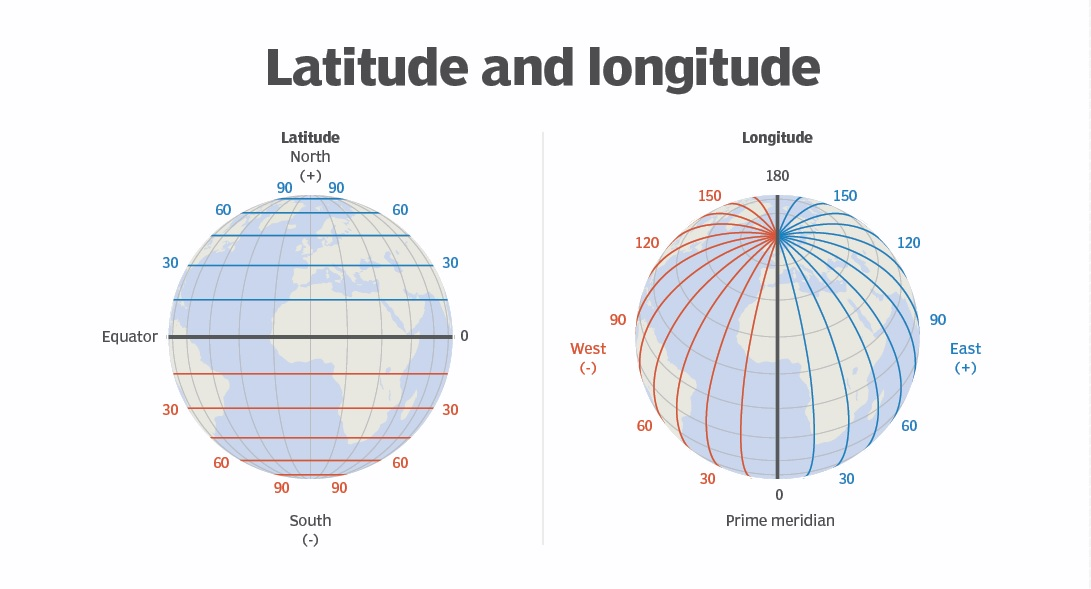
\includegraphics[width=0.85\linewidth]{gfx/m6l1_img002.jpeg}
\par\smallskip{\small \textbf{Hình:} Hệ tham chiếu tọa độ vĩ độ -- kinh độ. Nguồn: TechTarget.}
\end{figure}

\emph{Nguồn: TechTarget}

Khi xác định một vị trí trên CRS, quy ước chung là ghi vĩ độ trước, rồi đến kinh độ, theo dạng (vĩ độ, kinh độ). Có hai cách biểu diễn thông tin vĩ độ-kinh độ. Cách thứ nhất là độ, phút, giây (DMS). Ví dụ, tọa độ của New York theo DMS là (40° 43\textquotesingle{} 50.1960\textquotesingle\textquotesingle{} N, 73° 56\textquotesingle{} 6.8712\textquotesingle\textquotesingle{} W). Ký hiệu ° biểu thị độ, \textquotesingle{} biểu thị phút và \textquotesingle\textquotesingle{} biểu thị giây. Cách thứ hai là độ thập phân (DD). Tọa độ của New York theo DD là (40.730610, -73.935242).

DMS và DD có hai khác biệt chính. Khác biệt thứ nhất là DMS và DD dùng các ký hiệu khác nhau để biểu thị thông tin hướng của một vị trí. DMS dùng chữ cái để mô tả vị trí nằm ở bán cầu nào (N so với S; W so với E), còn DD dùng dấu + và - để mô tả bán cầu. Trong phương pháp DMS, tọa độ hướng của New York là (N, W). Trong phương pháp DD, tọa độ hướng của New York là (+,-). Chúng ta có thể dùng Hình 1 để hiểu cách phương pháp DD gán dấu +/-. Ở phần bên trái của hình, ta thấy nếu một vị trí nằm ở Bắc bán cầu thì dấu của vĩ độ là +; nếu vị trí nằm ở phía nam thì dấu của vĩ độ là -. Khái niệm này cũng áp dụng tương tự cho kinh độ.

Khác biệt thứ hai là DMS tính bằng độ, phút, giây còn DD tính bằng số thập phân. Chúng ta có thể dễ dàng chuyển đổi giữa hai phương pháp. Để chuyển từ DMS sang DD, trước tiên ta giữ nguyên số độ. Sau đó, ta chia số phút cho 60 và chia số giây cho 3600. Tiếp theo, ta cộng kết quả của hai phép chia này rồi cộng vào số độ. Con số cuối cùng chính là giá trị theo DD. Đôi khi, bán cầu của dữ liệu được chỉ ra bởi tên biến hoặc tiêu đề cột, và giá trị của các điểm dữ liệu trong bảng đều là số dương. Trong trường hợp này, chúng ta cần điều chỉnh thủ công giá trị của các điểm dữ liệu để biểu diễn đúng vị trí bán cầu theo phương pháp DD.

Trong Python, chúng ta sẽ dùng phương pháp DD để biểu diễn thông tin tọa độ. Bạn có thể dễ dàng tìm tọa độ DD của một địa điểm trên Google Maps.

\section{Các loại dữ liệu không gian địa lý}

Ở phần trước, chúng ta đã giới thiệu hệ tham chiếu tọa độ (CRS) kinh độ - vĩ độ. Trong phần về vị trí của đặc trưng, chúng ta đã nói rằng các loại dữ liệu địa lý khác nhau sẽ dùng những phương pháp khác nhau để biểu diễn thông tin vị trí. Có hai loại dữ liệu địa lý chính: dữ liệu raster và dữ liệu vector.

~~~~~~\textbf{Dữ liệu raster} chia một đặc trưng thành một hệ thống lưới. Mỗi ô lưới được gọi là một điểm ảnh (pixel) hoặc một ô (cell). Dữ liệu raster lưu trữ các thuộc tính của đặc trưng dựa trên từng điểm ảnh. Trong bài học về ảnh vệ tinh, chúng ta sẽ bàn kỹ hơn về dữ liệu raster.

~~~~~~\textbf{Dữ liệu vector} lưu trữ các thuộc tính của đặc trưng dựa trên hình dạng của đặc trưng. Một đặc trưng có thể có dạng điểm, dạng đường hoặc dạng đa giác. Trong bài học này, chúng ta sẽ tập trung vào dữ liệu vector.

Trước khi chuyển sang chủ đề tiếp theo về dữ liệu vector, hãy xem Hình 2 để hình dung trực quan sự khác biệt giữa hai loại dữ liệu địa lý này.

\textbf{Hình 2. Dữ liệu vector và dữ liệu raster}

\begin{figure}[H]
\centering
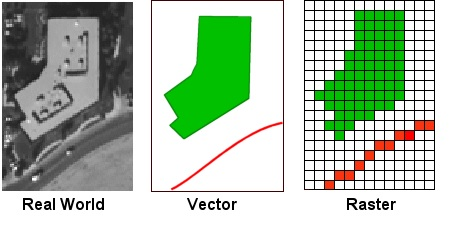
\includegraphics[width=0.85\linewidth]{gfx/m6l1_img003.jpeg}
\par\smallskip{\small \textbf{Hình:} Dữ liệu vector và dữ liệu raster biểu diễn thế giới thực. Nguồn: CUNY Hunter.}
\end{figure}

\emph{Nguồn: CUNY Hunter}

\section{Dữ liệu vector}

Ở phần trước, chúng ta đã trình bày cách biểu diễn một vị trí bằng CRS. Cho đến nay, ta mới chỉ đề cập đến vị trí điểm, tức là một chấm trên hệ tọa độ vĩ độ - kinh độ. Ngoài hình dạng điểm, chúng ta còn có thể đưa vào các hình dạng đường và hình dạng đa giác cùng với CRS. Hình 3 minh họa ví dụ về hình dạng điểm, hình dạng đường và hình dạng đa giác.

\textbf{Hình 3. Các hình dạng điểm, đường và đa giác}

\begin{figure}[H]
\centering
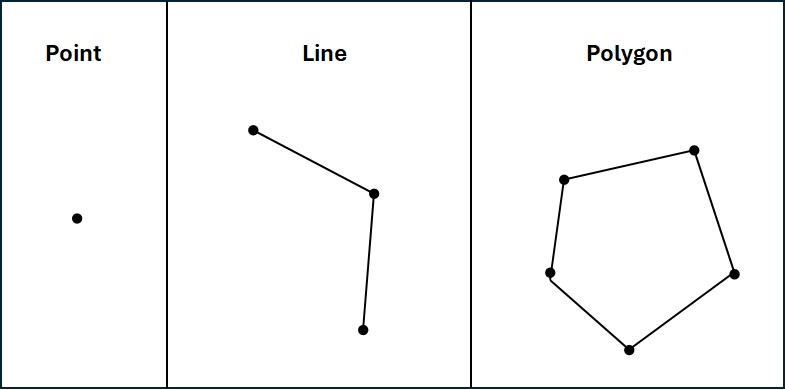
\includegraphics[width=0.85\linewidth]{gfx/m6l1_img001.jpeg}
\par\smallskip{\small \textbf{Hình:} Dữ liệu vector: điểm, đường và đa giác.}
\end{figure}

Ba hình dạng trên trong Hình 3 đều được cấu thành từ các điểm và các đường. Các điểm này được gọi là đỉnh (vertex). Vị trí của mỗi đỉnh có thể được biểu diễn bằng một cặp tọa độ vĩ độ - kinh độ. Nhờ có thông tin về hình dạng và thông tin về tọa độ của các đỉnh, chúng ta có thể xác định vị trí không gian địa lý của một đặc trưng trên hệ tọa độ vĩ độ - kinh độ. Trong dữ liệu vector, chúng ta lưu trữ thông tin hình dạng và thông tin tọa độ trong một biến gọi là \textbf{geometry}. Chính biến geometry này làm cho dữ liệu không gian địa lý khác biệt với dữ liệu dạng bảng truyền thống. Về định dạng dữ liệu không gian địa lý vector, có hai định dạng phổ biến: \textbf{GeoJSON} và \textbf{Shapefile}. Các tài liệu đọc bắt buộc sẽ giới thiệu rất ngắn gọn về hai định dạng dữ liệu này.

\section{Nguồn dữ liệu không gian địa lý và phần mềm phân tích}

Có nhiều cách để thu thập dữ liệu không gian địa lý. Một số nguồn thu thập dữ liệu gồm Hệ thống định vị toàn cầu (GPS), thiết bị đeo, điện thoại di động, viễn thám (vệ tinh) và Internet vạn vật (IoT), cùng nhiều nguồn khác.

Sau khi có dữ liệu không gian địa lý, các nhà nghiên cứu thường dùng \textbf{hệ thống thông tin địa lý (GIS)} để đọc và phân tích dữ liệu. Có nhiều GIS phổ biến, trả phí hoặc miễn phí, như ArcGIS hoặc QGIS. Các phần mềm này thường có sẵn các hàm đọc nhiều loại dữ liệu không gian địa lý khác nhau và các hàm trực quan hóa để trình bày dữ liệu.

\section{Ứng dụng của dữ liệu không gian địa lý}

Trong phần này, chúng ta sẽ sử dụng Python để minh họa cách lấy dữ liệu không gian địa lý từ nguồn dữ liệu trực tuyến, làm sạch dữ liệu để sẵn sàng cho phân tích và trực quan hóa dữ liệu.

Chúng ta sẽ lấy đường đi của bão Irene dọc theo bờ biển phía đông Hoa Kỳ làm ví dụ. Vào cuối tháng 8 năm 2011, bão Irene đã gây thiệt hại nghiêm trọng cho khu vực này của Hoa Kỳ. Chẳng hạn, khu vực hạ Manhattan của thành phố New York bị mất điện trong một tuần do cơn bão.

Trong ứng dụng này, chúng ta sẽ lấy dữ liệu về đường đi và sức gió của cơn bão từ Trung tâm Bão Quốc gia (National Hurricane Center - NHC) thuộc Cơ quan Quản lý Khí quyển và Đại dương Quốc gia Hoa Kỳ (National Oceanic and Atmospheric Administration - NOAA). Chúng ta sẽ lấy dữ liệu và vẽ đường đi của cơn bão lên bản đồ. Trong phần minh họa này, chúng ta cũng sẽ trình bày cách chồng các thông tin khác nhau lên bản đồ. Chúng ta sẽ chồng ranh giới các bang của Hoa Kỳ lên bản đồ để cho thấy những bang nào chịu ảnh hưởng của cơn bão này.

Gói Python chính dùng để phân tích dữ liệu không gian địa lý là geopandas. Geopandas là phiên bản dữ liệu không gian địa lý của pandas. Gói này có thể xử lý nhiều loại dữ liệu không gian địa lý mà chúng ta đã đề cập ở các phần trước. Sau đó, chúng ta sẽ dùng gói folium để trực quan hóa đường đi của cơn bão. Chúng ta bắt đầu thôi.

\subsection{Tải các gói Python}

Chúng ta sẽ cần một số gói cho phần minh họa này.

\begin{lstlisting}[language=Python,escapeinside={(*@}{@*)}]
!pip install fiona
\end{lstlisting}

\begin{lstlisting}[language=Python,escapeinside={(*@}{@*)}]
!pip install geopandas
\end{lstlisting}

\begin{lstlisting}[language=Python,escapeinside={(*@}{@*)}]
pip install install-jdk
\end{lstlisting}

\begin{lstlisting}[language=Python,escapeinside={(*@}{@*)}]
import jdk
from jdk.enums import OperatingSystem, Architecture

jdk.install('11', operating_system=OperatingSystem.LINUX)
\end{lstlisting}

Output:

\begin{lstlisting}[escapeinside={(*@}{@*)}]
'/root/.jdk/jdk-11.0.25+9'
\end{lstlisting}

\begin{lstlisting}[language=Python,escapeinside={(*@}{@*)}]
import os
jdk_version = 'jdk-11.0.25+9' #change with your version 
os.environ['JAVA_HOME'] = '/root/.jdk/jdk-11.0.25+9'
os.environ['PATH'] = f"{os.environ.get('PATH')}:{os.environ.get('JAVA_HOME')}/bin"
\end{lstlisting}

\begin{lstlisting}[language=Python,escapeinside={(*@}{@*)}]
# (*@Nhập@*) (*@các@*) (*@gói@*) cho (*@ứng@*) (*@dụng@*) (*@này@*)
# pandas (*@dùng@*) (*@để@*) (*@xử@*) (*@lý@*) dataframe (*@và@*) geopandas (*@dùng@*) (*@để@*) (*@xử@*) (*@lý@*) geodataframe
# fiona (*@dùng@*) (*@để@*) (*@đọc@*) (*@hoặc@*) ghi (*@nhiều@*) (*@định@*) (*@dạng@*) (*@dữ@*) (*@liệu@*) (*@không@*) gian (*@địa@*) (*@lý@*)
# urllib (*@dùng@*) (*@để@*) (*@lấy@*) (*@dữ@*) (*@liệu@*) (*@trên@*) internet (*@bằng@*) url
# zipfile (*@dùng@*) (*@để@*) (*@giải@*) (*@nén@*) (*@tệp@*) zip
import os
import pandas as pd
import geopandas as gpd
import fiona
import urllib.request
import zipfile
\end{lstlisting}

\subsection{Dữ liệu về cơn bão Irene}

Dữ liệu về đường đi của cơn bão nằm trong một tệp PDF. Do đó, chúng ta cần cài đặt gói tabula để xử lý các tệp PDF.

\begin{lstlisting}[language=Python,escapeinside={(*@}{@*)}]
pip install tabula-py
\end{lstlisting}

\begin{lstlisting}[language=Python,escapeinside={(*@}{@*)}]
# Import tabula package for PDF handling
import tabula
\end{lstlisting}

Tiếp theo, hãy lấy tệp PDF từ trang web của Trung tâm Bão Quốc gia Hoa Kỳ (National Hurricane Center, NHC).

\begin{lstlisting}[language=Python,escapeinside={(*@}{@*)}]
# Retrieve PDF file from NHC website
url = "https://www.nhc.noaa.gov/data/tcr/AL092011_Irene.pdf"

irene_pdf, _ = urllib.request.urlretrieve(url)
\end{lstlisting}

Sau đó, chúng ta sẽ dùng một phương thức của gói tabula để chuyển tệp PDF thành tệp csv.

\begin{lstlisting}[language=Python,escapeinside={(*@}{@*)}]
# Convert PDF file to csv file, and then a pandas dataframe
tabula.convert_into(irene_pdf, "irene.csv", output_format="csv", stream=True, pages = 9)
irene_1 = pd.read_csv("irene.csv")
irene_1
\end{lstlisting}

Từ kết quả của đoạn mã trước, ta thấy hàng thứ hai không chứa giá trị dữ liệu. Đó là các đơn vị đo lường/thông tin của từng biến. Ví dụ, đơn vị đo của tốc độ gió là hải lý/giờ (knot, kt). Ngoài ra, hàng cuối cùng cũng không có giá trị dữ liệu nào. Chúng ta sẽ loại bỏ hai hàng này.

\begin{lstlisting}[language=Python,escapeinside={(*@}{@*)}]
# Drop rows with measurement units or no data values
irene_1.drop([0,40], inplace = True)
irene_1
\end{lstlisting}

Tiếp theo, hãy chuyển các biến số sang kiểu số thực (float).

\begin{lstlisting}[language=Python,escapeinside={(*@}{@*)}]
# Correct data types for numeric variables
convert_dict = {'Date/Time': str,
                'Latitude': float,
                'Longitude': float,
                'Pressure': float,
                'Wind Speed': float
                }

irene_1 = irene_1.astype(convert_dict)
print(irene_1.dtypes)
\end{lstlisting}

Kết quả:

\begin{lstlisting}[escapeinside={(*@}{@*)}]
Date/Time      object
Latitude      float64
Longitude     float64
Pressure      float64
Wind Speed    float64
Unnamed: 5     object
dtype: object
\end{lstlisting}

\subsection{Tạo biến ngày-giờ}

Tiếp theo, ta thấy biến ngày/giờ không chứa thông tin về tháng và năm. Do đó, chúng ta sẽ tạo một biến ngày/giờ mới để cung cấp thông tin ngày/giờ đầy đủ.

\begin{lstlisting}[language=Python,escapeinside={(*@}{@*)}]
# Create a new Date Time variable to contain month and year information
irene_1[["Date","Time"]] = irene_1["Date/Time"].str.split(" / ", expand = True)
irene_1["Date_Time"] = "08/" + irene_1["Date"] + "/2011/" + irene_1["Time"]
irene_1.set_index("Date_Time")
irene_1
\end{lstlisting}

\subsection{Đảm bảo dữ liệu không gian địa lý chính xác}

Chúng ta cũng nhận thấy rằng các giá trị kinh độ trong bộ dữ liệu đều là số dương. Tuy nhiên, hướng của kinh độ là "W" (Tây). Dựa trên Hình 1 ở mục 3, các số liệu kinh độ lẽ ra phải là số âm. Do đó, chúng ta cần thêm dấu âm vào trước tất cả các giá trị của biến kinh độ để phản ánh đúng vị trí.

\begin{lstlisting}[language=Python,escapeinside={(*@}{@*)}]
# Adjust Longitude value to correctly reflect the geolocation
irene_1['Longitude'] = 0 - irene_1['Longitude']
\end{lstlisting}

\begin{lstlisting}[language=Python,escapeinside={(*@}{@*)}]
# Select the variables we are interest for next steps
irene_2 = irene_1[["Date_Time","Longitude","Latitude","Wind Speed"]]
\end{lstlisting}

\subsection{Chuyển đổi sang Geodataframe}

Bây giờ chúng ta đã có một dataframe hoàn chỉnh cho đường đi của bão Irene. Để chuyển dataframe này thành dataframe không gian địa lý, chúng ta cần tạo một biến hình học (geometry), như đã giải thích ở phần trước. Chúng ta sẽ dùng một phương thức của geopandas để tạo biến này. Một trong các tham số trong đoạn mã dưới đây là "EPSG:4326", là mã định danh của hệ kinh độ - vĩ độ mà chúng ta đã quen thuộc. Hãy nhớ rằng có nhiều hệ tham chiếu tọa độ (CRS) khác nhau, nhưng chúng ta sẽ tiếp tục với hệ được sử dụng phổ biến này.

\begin{lstlisting}[language=Python,escapeinside={(*@}{@*)}]
# (*@Tạo@*) (*@biến@*) (*@vị@*) (*@trí@*) (*@địa@*) (*@lý@*)
geometry = gpd.points_from_xy(irene_2.Longitude, irene_2.Latitude, crs="EPSG:4326")
\end{lstlisting}

Bây giờ hãy chuyển pandas dataframe hiện tại thành geodataframe.

\begin{lstlisting}[language=Python,escapeinside={(*@}{@*)}]
# (*@Chuyển@*) dataframe (*@hiện@*) (*@tại@*) (*@thành@*) geodataframe (*@với@*) (*@biến@*) geometry
irene_3 = gpd.GeoDataFrame(
    irene_2, geometry=geometry, crs="EPSG:4326"
)
\end{lstlisting}

Tuyệt vời! Bây giờ chúng ta đã có một geodataframe. Hãy xem năm dòng đầu tiên của dataframe này.

\begin{lstlisting}[language=Python,escapeinside={(*@}{@*)}]
irene_3.head()
\end{lstlisting}

Output:

\begin{lstlisting}[escapeinside={(*@}{@*)}]
         Date_Time  Longitude  Latitude  Wind Speed            geometry
1  08/21/2011/0000      -59.0      15.0        45.0      POINT (-59 15)
2  08/21/2011/0600      -60.6      16.0        45.0    POINT (-60.6 16)
3  08/21/2011/1200      -62.2      16.8        45.0  POINT (-62.2 16.8)
4  08/21/2011/1800      -63.7      17.5        50.0  POINT (-63.7 17.5)
5  08/22/2011/0000      -65.0      17.9        60.0    POINT (-65 17.9)
\end{lstlisting}

Trong biến geometry của geodataframe ở trên, chúng ta có các hình dạng điểm và cặp tọa độ của chúng trên bản đồ. Hãy xác nhận kiểu của dataframe mới này.

\begin{lstlisting}[language=Python,escapeinside={(*@}{@*)}]
type(irene_3)
\end{lstlisting}

Output:

\begin{lstlisting}[escapeinside={(*@}{@*)}]
geopandas.geodataframe.GeoDataFrame
\end{lstlisting}

Và hãy kiểm tra biến geometry của chúng ta.

\begin{lstlisting}[language=Python,escapeinside={(*@}{@*)}]
type(irene_3['geometry'])
\end{lstlisting}

Output:

\begin{lstlisting}[escapeinside={(*@}{@*)}]
geopandas.geoseries.GeoSeries
\end{lstlisting}

Về cơ bản, geodataframe hoạt động giống như pandas dataframe. Do đó, chúng ta có thể áp dụng các phương thức và phân tích tương tự của pandas cho geopandas. Sau đây là một ví dụ.

\begin{lstlisting}[language=Python,escapeinside={(*@}{@*)}]
print("Mean wind speed of Hurricane Irene is {} knots and it can go up to {} knots maximum".format(round(irene_2['Wind Speed'].mean(),4),
                                                                                         irene_2['Wind Speed'].max())+".")
\end{lstlisting}

Output:

\begin{lstlisting}[escapeinside={(*@}{@*)}]
Mean wind speed of Hurricane Irene is 69.6154 knots and it can go up to 105.0 knots maximum.
\end{lstlisting}

\subsection{Dữ liệu ranh giới các bang của Hoa Kỳ}

Trước khi vẽ đường đi của bão Irene lên bản đồ, chúng ta muốn thêm một lớp ranh giới các bang của Hoa Kỳ vào bản đồ. Khi trực quan hóa ranh giới các bang cùng với đường đi của bão Irene, chúng ta có thể biết những bang nào bị ảnh hưởng bởi cơn bão này. Chúng ta sẽ lấy tệp ranh giới các bang từ trang web của Cục Điều tra Dân số Hoa Kỳ (United States Census Bureau). Đây là một shapefile được nén dạng zip. Trước tiên, chúng ta cần nhập một gói để giải nén tệp.

\begin{lstlisting}[language=Python,escapeinside={(*@}{@*)}]
# (*@Nhập@*) (*@gói@*) (*@giải@*) (*@nén@*) (*@tệp@*)
from zipfile import ZipFile
\end{lstlisting}

\begin{lstlisting}[language=Python,escapeinside={(*@}{@*)}]
# (*@Lấy@*) shapefile (*@các@*) bang (*@của@*) Hoa (*@Kỳ@*) (*@từ@*) United States Census Bureau
us_state_url = "	http://www2.census.gov/geo/tiger/TIGER2012/STATE/tl_2012_us_state.zip"

us_state_shape_zip, _ = urllib.request.urlretrieve(us_state_url)
\end{lstlisting}

\begin{lstlisting}[language=Python,escapeinside={(*@}{@*)}]
# (*@Giải@*) (*@nén@*) shapefile (*@và@*) (*@đặt@*) (*@tên@*) (*@mới@*) (*@là@*) "us_state_shape"
with ZipFile(us_state_shape_zip, 'r') as zObject:

    zObject.extractall("us_state_shape")
\end{lstlisting}

Sau khi giải nén tệp, chúng ta sẽ dùng phương thức read\_file của geopandas để đọc tệp này thành một geodataframe nhằm xử lý dữ liệu tiếp theo.

\begin{lstlisting}[language=Python,escapeinside={(*@}{@*)}]
# (*@Đọc@*) shapefile (*@vào@*) (*@một@*) geodataframe
us_state_shape_g = gpd.read_file("us_state_shape")
\end{lstlisting}

\begin{lstlisting}[language=Python,escapeinside={(*@}{@*)}]
# (*@Kiểm@*) tra (*@siêu@*) (*@dữ@*) (*@liệu@*) (*@của@*) geodataframe (*@mới@*)
us_state_shape_g.info()
\end{lstlisting}

Output:

\begin{lstlisting}[escapeinside={(*@}{@*)}]
<class 'geopandas.geodataframe.GeoDataFrame'>
RangeIndex: 56 entries, 0 to 55
Data columns (total 15 columns):
 #   Column    Non-Null Count  Dtype   
---  ------    --------------  -----   
 0   REGION    56 non-null     object  
 1   DIVISION  56 non-null     object  
 2   STATEFP   56 non-null     object  
 3   STATENS   56 non-null     object  
 4   GEOID     56 non-null     object  
 5   STUSPS    56 non-null     object  
 6   NAME      56 non-null     object  
 7   LSAD      56 non-null     object  
 8   MTFCC     56 non-null     object  
 9   FUNCSTAT  56 non-null     object  
 10  ALAND     56 non-null     int64   
 11  AWATER    56 non-null     int64   
 12  INTPTLAT  56 non-null     object  
 13  INTPTLON  56 non-null     object  
 14  geometry  56 non-null     geometry
dtypes: geometry(1), int64(2), object(12)
memory usage: 6.7+ KB
\end{lstlisting}

\begin{lstlisting}[language=Python,escapeinside={(*@}{@*)}]
# (*@Kiểm@*) tra (*@vài@*) (*@dòng@*) (*@đầu@*) (*@của@*) geodataframe (*@mới@*)
us_state_shape_g.head()
\end{lstlisting}

Output:

\begin{lstlisting}[escapeinside={(*@}{@*)}]
  REGION DIVISION STATEFP   STATENS GEOID STUSPS        NAME LSAD  MTFCC   
0      4        9      15  01779782    15     HI      Hawaii   00  G4000  \
1      3        7      05  00068085    05     AR    Arkansas   00  G4000   
2      4        8      35  00897535    35     NM  New Mexico   00  G4000   
3      4        8      30  00767982    30     MT     Montana   00  G4000   
4      1        2      36  01779796    36     NY    New York   00  G4000   

  FUNCSTAT         ALAND       AWATER     INTPTLAT      INTPTLON   
0        A   16634247483  11678744699  +19.8097670  -155.5061027  \
1        A  134772564356   2959210006  +34.8955256  -092.4446262   
2        A  314161109357    756438507  +34.4346843  -106.1316181   
3        A  376963571188   3868564895  +47.0511771  -109.6348174   
4        A  122057936950  19238848209  +42.9133974  -075.5962723   

                                            geometry  
0  MULTIPOLYGON (((-155.96333 19.08159, -155.9634...  
1  POLYGON ((-94.46025 34.53838, -94.46026 34.543...  
2  POLYGON ((-109.04616 34.57929, -109.04616 34.5...  
3  POLYGON ((-114.33289 46.66076, -114.33367 46.6...  
4  MULTIPOLYGON (((-79.64546 41.99886, -79.6498 4...
\end{lstlisting}

\subsection{Trực quan hóa dữ liệu không gian địa lý}

Bây giờ chúng ta đã có tệp về đường đi của bão Irene và tệp về ranh giới các bang của Hoa Kỳ. Cả hai đều ở dạng geodataframe. Chúng ta có thể đưa toàn bộ thông tin vào một bản đồ để trực quan hóa. Chúng ta sẽ dùng gói folium để vẽ bản đồ, rồi thêm ranh giới các bang của Hoa Kỳ và đường đi của cơn bão vào bản đồ.

\begin{lstlisting}[language=Python,escapeinside={(*@}{@*)}]
pip install folium
\end{lstlisting}

\begin{lstlisting}[language=Python,escapeinside={(*@}{@*)}]
# Import a mapping library
import folium
\end{lstlisting}

Tuyệt vời! Bây giờ là lúc đưa thông tin lên bản đồ.

\begin{lstlisting}[language=Python,escapeinside={(*@}{@*)}]
# (*@Vẽ@*) (*@đường@*) (*@đi@*) (*@của@*) (*@bão@*) Irene (*@và@*) (*@các@*) (*@thông@*) tin (*@khác@*) (*@lên@*) (*@bản@*) (*@đồ@*)

# (*@Đầu@*) (*@tiên@*), (*@tạo@*) (*@bản@*) (*@đồ@*) (*@nền@*)
map = folium.Map(location=[30,-102], zoom_start=4, control_scale=True)

# Sau (*@đó@*) (*@thêm@*) (*@lớp@*) (*@đầu@*) (*@tiên@*) (*@là@*) ranh (*@giới@*) (*@các@*) bang (*@của@*) Hoa (*@Kỳ@*) (*@vào@*) (*@bản@*) (*@đồ@*)
folium.GeoJson(us_state_shape_g).add_to(map)

# (*@Tiếp@*) theo (*@thêm@*) (*@đường@*) di (*@chuyển@*) (*@của@*) (*@cơn@*) (*@bão@*) (*@vào@*) (*@bản@*) (*@đồ@*). (*@Chúng@*) ta (*@dùng@*) (*@một@*) (*@chấm@*) (*@đỏ@*) (*@để@*) (*@biểu@*) (*@diễn@*) (*@vị@*) (*@trí@*) (*@của@*) (*@cơn@*) (*@bão@*) (*@tại@*) (*@một@*) (*@ngày@*)/(*@giờ@*) (*@cụ@*) (*@thể@*). Sau (*@đó@*) (*@thêm@*) (*@một@*) (*@hộp@*) (*@thông@*) tin (*@và@*) (*@một@*) (*@hộp@*) popup. (*@Nếu@*) di (*@chuột@*) (*@đến@*) (*@chấm@*) (*@đỏ@*), (*@bản@*) (*@đồ@*) (*@sẽ@*) (*@hiển@*) (*@thị@*) (*@ngày@*)/(*@giờ@*) (*@gắn@*) (*@với@*) (*@vị@*) (*@trí@*) (*@đó@*) (*@và@*) (*@tốc@*) (*@độ@*) (*@gió@*).
folium.GeoJson(irene_3,
               marker=folium.Circle(radius=2000, fill_color="red", fill_opacity=0.4, color="red", weight=5),
              tooltip=folium.GeoJsonTooltip(fields=["Date_Time","Wind Speed"]),
              popup=folium.GeoJsonPopup(fields=["Date_Time","Wind Speed"]),).add_to(map)

map
\end{lstlisting}

Output:

\begin{lstlisting}[escapeinside={(*@}{@*)}]
<folium.folium.Map at 0x73b5d8373dd0>
\end{lstlisting}

Xong rồi! Chúng ta vừa tạo một bản đồ chồng lớp ranh giới các bang của Hoa Kỳ và đường đi của bão Irene. Ở góc trên bên trái của bản đồ có một biểu tượng để phóng to và thu nhỏ. Ranh giới các bang của Hoa Kỳ được thể hiện bằng các đường liền màu xanh lam trên bản đồ. Đường đi của bão Irene được biểu diễn bằng một chuỗi các chấm đỏ. Khi di chuột qua một chấm đỏ, một hộp thông tin sẽ hiện ra, cung cấp thông tin về ngày/giờ và tốc độ gió. Với bản đồ này, chúng ta thấy bão Irene đi qua hầu hết các bang phía bắc dọc bờ biển phía đông Hoa Kỳ. Tốc độ gió đạt mạnh nhất khi cơn bão đi qua khu vực giữa Cộng hòa Dominica và Bahamas. Tốc độ gió giảm đáng kể sau khi bão đổ bộ vào đất liền.

\section{Kết luận}

Trong bài học này, trước hết chúng ta đã giải thích dữ liệu không gian địa lý là gì. Chúng ta đã giới thiệu khái niệm sử dụng hệ tham chiếu tọa độ (CRS) để cung cấp thông tin định vị địa lý trên bề mặt Trái Đất. Chúng ta cũng đã giải thích dữ liệu vector và các định dạng dữ liệu phổ biến của nó. Sau đó, chúng ta đã trình bày một ứng dụng dữ liệu không gian địa lý đơn giản bằng Python. Thông qua ứng dụng này, chúng ta đã học cách xử lý các loại dữ liệu không gian địa lý khác nhau. Chúng ta cũng đã học cách phủ dữ liệu đã xử lý lên bản đồ để trực quan hóa dữ liệu.

\section{Tài liệu tham khảo}

\begin{enumerate}
\def\labelenumi{\arabic{enumi}.}
\item
  Awati, Rahul. "Latitude and Longitude." Informa TechTarget, August 2022. https://www.techtarget.com/whatis/definition/latitude-and-longitude.
\end{enumerate}

\begin{lstlisting}[language=Python,escapeinside={(*@}{@*)}]

\end{lstlisting}

\chapter{Đọc thêm 1: GeoJSON}
\label{ch:M6L1DocThem1}

\section{Thông tin nguồn}

\begin{itemize}
  \item \textbf{Nguồn:} GeoJSON. \url{https://geojson.org}
  \item \textbf{Phần cần đọc:} Toàn bộ trang
  \item \textbf{Ghi chú:} bản chuyển ngữ tiếng Việt súc tích, bám cấu trúc nguồn (giữ nguyên tiêu đề, công thức, số liệu, bảng, chú thích và danh mục tài liệu tham khảo).
\end{itemize}

GeoJSON là một định dạng dùng để mã hóa nhiều loại cấu trúc dữ liệu địa lý.

\begin{lstlisting}[escapeinside={(*@}{@*)}]
{
    "type": "Feature",
    "geometry": {
      "type": "Point",
      "coordinates": [125.6, 10.1]
    },
    "properties": {
      "name": "Dinagat Islands"
    }
}
\end{lstlisting}

GeoJSON hỗ trợ các kiểu hình học sau: Point, LineString, Polygon, MultiPoint, MultiLineString và MultiPolygon. Đối tượng hình học kèm thuộc tính bổ sung là đối tượng Feature. Tập hợp các feature được chứa trong đối tượng FeatureCollection.

\subsection{Đặc tả GeoJSON (RFC 7946)}

Năm 2015, Internet Engineering Task Force (IETF) phối hợp với các tác giả đặc tả gốc đã thành lập một nhóm làm việc (WG) về GeoJSON nhằm chuẩn hóa định dạng này. RFC 7946 được công bố vào tháng 8 năm 2016 và là đặc tả chuẩn mới của định dạng GeoJSON, thay thế đặc tả GeoJSON năm 2008.

\chapter{Đọc thêm 2: Shapefile là gì? (Temple University)}
\label{ch:M6L1DocThem2}

\section{Thông tin nguồn}

\begin{itemize}
  \item \textbf{Nguồn:} Temple University Libraries. ``What are Shapefiles?''
  \item \textbf{Phần cần đọc:} Toàn bộ trang
  \item \textbf{Ghi chú:} bản chuyển ngữ tiếng Việt súc tích, bám cấu trúc nguồn (giữ nguyên tiêu đề, công thức, số liệu, bảng, chú thích và danh mục tài liệu tham khảo).
\end{itemize}

Hướng dẫn tìm hiểu, tìm kiếm và sử dụng shapefile.

\subsubsection{Shapefile là gì?}

Shapefile (SHP) là định dạng lưu trữ dữ liệu vector, dùng để lưu vị trí, hình dạng và thuộc tính của các đối tượng địa lý. Định dạng này do ESRI phát triển nên đôi khi được gọi là "ESRI shapefile". Shapefile là loại tệp GIS (hệ thống thông tin địa lý) phổ biến nhất và hiện được chấp nhận làm định dạng chuẩn của toàn ngành.

Định dạng shapefile mô tả hình học và thuộc tính của các đối tượng có tham chiếu địa lý trong ba tệp trở lên với các phần mở rộng riêng, và các tệp này cần được lưu trong cùng một không gian làm việc của dự án.

Có ba tệp bắt buộc:

\begin{itemize}
\item
  .shp là tệp Esri bắt buộc, cung cấp hình học cho các đối tượng. Mỗi shapefile có một tệp .shp riêng chứa dữ liệu vector không gian, chẳng hạn điểm, đường và đa giác trên bản đồ.
\item
  .shx là tệp chỉ mục vị trí hình dạng bắt buộc của Esri và AutoCAD, dùng để tìm kiếm tiến và lùi.
\item
  .dbf là tệp cơ sở dữ liệu chuẩn, dùng để lưu dữ liệu thuộc tính và mã định danh đối tượng (object ID). Tệp .dbf là bắt buộc đối với shapefile và có thể mở bằng Microsoft Access hoặc Excel.
\end{itemize}

Để có mô tả đầy đủ hơn về định dạng shapefile, xem ESRI White Paper (tháng 7/1998): ESRI Shapefile Technical Description.

% ---- Lesson 2 ----
\chapter{Ảnh vệ tinh}
\label{ch:M6L2LessonNotes}

\section*{Lesson Notes}

MÔ-ĐUN 6 \textbar{} BÀI 2

\section{Tài liệu đọc bắt buộc}

Các tài liệu đọc bắt buộc của chương trình này đều là tài liệu truy cập mở, nghĩa là bạn có thể truy cập miễn phí. Liên kết trong phần trích dẫn sẽ đưa bạn trực tiếp đến tài liệu hoặc đến trang cho phép tải xuống.

\begin{enumerate}
\def\labelenumi{\arabic{enumi}.}
\item
  NASA. "Remote Sensing." \emph{NASA EarthData}. https://www.earthdata.nasa.gov/learn/backgrounders/remote-sensing\#spectral-resolution
\end{enumerate}

\begin{itemize}
\item
  \textbf{Các trang bắt buộc:} Toàn bộ trang web
\item
  \textbf{Thời gian đọc ước tính:} 30 phút
\end{itemize}

\begin{enumerate}
\def\labelenumi{\arabic{enumi}.}
\setcounter{enumi}{1}
\item
  NASA Goddard. "9 Things about Landsat 9." \emph{YouTube}, đăng tải ngày 26 tháng 9 năm 2021, https://www.youtube.com/watch?v=DGE-N8\_LQBo.
\end{enumerate}

\begin{itemize}
\item
  \textbf{Các trang bắt buộc:} Toàn bộ video
\item
  \textbf{Thời gian xem ước tính:} 6 phút
\end{itemize}

MODULE 6 \textbar{} BÀI 2

\section{Ảnh vệ tinh}

{\small
\begin{longtable}[]{@{}ll@{}}
\toprule\noalign{}
\endhead
\bottomrule\noalign{}
\endlastfoot
\textbf{Thời gian đọc} & 60 phút \\
\textbf{Kiến thức nền} & Python cơ bản \\
\textbf{Từ khóa} & Viễn thám, Phổ điện từ, Độ phân giải không gian \\
& \\
& \\
\end{longtable}
}

\section{Giới thiệu}

Trong bài học này, chúng ta sẽ làm quen với một loại dữ liệu mà chúng ta chưa đề cập: \textbf{ảnh vệ tinh}. Theo truyền thống, ảnh vệ tinh là loại dữ liệu được sử dụng trong các ngành khoa học tự nhiên hoặc lĩnh vực quốc phòng. Tuy nhiên, trong những năm gần đây, ngày càng nhiều nhà phân tích tài chính sử dụng ảnh vệ tinh để phân tích, với hy vọng thu được thêm những hiểu biết bổ sung bên cạnh phân tích tài chính truyền thống để đưa ra các quyết định tài chính tốt hơn. Nội dung của bài học này dựa trên thông tin trong các tài liệu đọc bắt buộc của bạn. Trước hết, chúng ta sẽ giới thiệu những kiến thức cơ bản về ảnh vệ tinh. Sau đó, chúng ta sẽ trình bày ngắn gọn một số ứng dụng của ảnh vệ tinh trong phân tích tài chính. Cuối cùng, chúng ta sẽ sử dụng Google Earth Engine (GEE) để truy cập một số ảnh vệ tinh và đưa ra các ví dụ về cách sử dụng ảnh vệ tinh cho phân tích.

\section{Ứng dụng tài chính của ảnh vệ tinh}

Trong phần này, chúng ta sẽ tìm hiểu cách đưa ảnh vệ tinh vào làm một phần dữ liệu cho phân tích tài chính.

Một trong những trường hợp nổi tiếng nhất về việc sử dụng ảnh vệ tinh trong phân tích tài chính là đếm số lượng ô tô ra vào bãi đỗ xe của các cửa hàng Walmart trong một khoảng thời gian. Các nhà phân tích tài chính dùng thông tin này như một chỉ báo thay thế (proxy) cho lưu lượng khách đến cửa hàng để ước tính doanh số của cửa hàng trong một giai đoạn cụ thể. Đây chính là ứng dụng đầu tiên của ảnh vệ tinh.

\subsection{Giám sát hoạt động kinh tế của một địa điểm}

Ví dụ về bãi đỗ xe của Walmart là một ứng dụng kinh điển của ảnh vệ tinh. Một ví dụ khác là dùng ảnh vệ tinh để giám sát lưu lượng tàu container tại một kênh đào lớn hoặc một cảng lớn nhằm phát hiện các tắc nghẽn có thể xảy ra trong chuỗi cung ứng. Chúng ta cũng có thể dùng ảnh vệ tinh để giám sát các nhà máy nhằm đánh giá mức sản lượng tiềm năng tại một thời điểm nhất định. Ngoài ra, chúng ta còn có thể giám sát một mỏ khai thác để theo dõi sản lượng hàng hóa cơ bản (commodity).

\subsection{Theo dõi sản lượng cây trồng}

Chúng ta có thể dùng ảnh vệ tinh để xem một loại cây trồng nhất định, như lúa mì hoặc ngô, có khỏe mạnh hay không. Từ thông tin này, các nhà phân tích tài chính có thể ước tính thị trường sẽ dư cung hay thiếu hụt nguồn cung của loại cây trồng đó và giao dịch dựa trên thông tin này. Thông thường, chúng ta sẽ dùng kết hợp các dải hồng ngoại để thực hiện phân tích này.

\subsection{Điều tra thiệt hại do thiên tai}

Hiện nay, các công ty bảo hiểm sử dụng ảnh vệ tinh để đánh giá thiệt hại do lũ lụt hoặc cháy rừng. Phương pháp thu thập thông tin thiệt hại này hiệu quả hơn so với phương pháp truyền thống là đến tận hiện trường. Thứ nhất, phương pháp truyền thống có thể cần vài tháng để thu thập dữ liệu, trong khi dùng ảnh vệ tinh chỉ mất vài giờ. Thứ hai, nhiều khu vực bị thiệt hại thường không thể tiếp cận được sau thảm họa, nên không thể áp dụng phương pháp truyền thống. Với công nghệ ảnh vệ tinh mới này, các công ty bảo hiểm có thể xử lý yêu cầu bồi thường nhanh hơn và tiết kiệm chi phí hơn.

\subsection{Những hạn chế khi sử dụng ảnh vệ tinh cho phân tích tài chính}

Hiện nay, đối với công chúng nói chung, có một số vấn đề khi sử dụng ảnh vệ tinh cho phân tích đầu tư.

~~~(A) Độ phân giải thời gian của ảnh vệ tinh công khai có thể dài. Ví dụ, Landsat 9 có độ phân giải thời gian là 8 ngày. Nhiều vệ tinh thương mại cung cấp ảnh vệ tinh với độ phân giải thời gian ngắn, chẳng hạn một ngày. Tuy nhiên, chúng rất đắt đỏ.

~~~(B) Xử lý lượng lớn ảnh vệ tinh đòi hỏi hạ tầng máy tính mạnh, thứ mà cá nhân thường không có.

~~~(C) Xử lý ảnh vệ tinh thô và chuyển chúng thành ảnh có thể sử dụng đòi hỏi được đào tạo chuyên môn.

Do những hạn chế này khi dùng ảnh vệ tinh để phân tích, hiện có nhiều công ty cung cấp dịch vụ truy cập các nền tảng phân tích ảnh vệ tinh của họ theo hình thức đăng ký thuê bao. Các công ty này thu thập ảnh vệ tinh công khai và tư nhân, xử lý chúng, rồi tải lên nền tảng của mình. Các nền tảng này thường tích hợp khả năng học máy để phân tích. Tuy nhiên, phí truy cập các nền tảng này cao, nên chỉ các quỹ phòng hộ (hedge fund) hoặc các công ty đầu tư lớn mới có thể sử dụng. Lấy ví dụ việc dùng lưu lượng ô tô tại bãi đỗ xe của các cửa hàng bán lẻ làm chỉ báo cho giao dịch cổ phiếu. Đây vẫn là một chiến lược giao dịch sinh lời, nhưng chỉ các quỹ phòng hộ mới tiếp cận được thông tin này.

\section{Kiến thức cơ bản về ảnh vệ tinh}

\subsection{Viễn thám}

Trước khi bàn về ảnh vệ tinh, chúng ta cần giới thiệu một vài khái niệm. Khái niệm đầu tiên là viễn thám. \textbf{Viễn thám} (remote sensing) là hoạt động sử dụng các vệ tinh quan sát Trái Đất hoặc máy bay được trang bị cảm biến để thu nhận hình ảnh và các thông tin khác về bề mặt Trái Đất từ trên cao.

Các cảm biến trên vệ tinh đo \textbf{bức xạ điện từ (EMR)}, vốn trước hết được phát ra từ Mặt Trời. Khi đến bề mặt Trái Đất, bức xạ này được phản xạ trở lại các cảm biến trên vệ tinh. Hình 1 dưới đây minh họa đường đi của EMR.

\textbf{Hình 1: Minh họa cách vệ tinh đo EMR phản xạ từ bề mặt Trái Đất}

Phỏng theo: NASA EarthData. "What Is Remote Sensing?" 10 December 2024. https://www.earthdata.nasa.gov/learn/backgrounders/remote-sensing.

\subsection{Phổ điện từ}

EMR là một dạng năng lượng truyền đi theo sóng. Tuy nhiên, các sóng này không đồng nhất; chúng có các bước sóng khác nhau. Bước sóng của một sóng được đo bằng khoảng cách giữa hai đỉnh sóng. Nếu một sóng có bước sóng ngắn hơn các sóng khác thì sóng này có tần số cao hơn, vì sóng dao động lên xuống rồi lại lên nhanh hơn.

Chúng ta nhóm các sóng có bước sóng tương tự nhau thành một dải gọi là \textbf{phổ (spectrum)}. Hình 2 bên dưới cho thấy cách chúng ta nhóm các sóng thành các phổ hay dải khác nhau theo bước sóng của chúng.

\textbf{Hình 2: Phổ bức xạ điện từ}

Nguồn: NASA EarthData. "What Is Remote Sensing?" 10 December 2024. https://www.earthdata.nasa.gov/learn/backgrounders/remote-sensing.

Hình 2 biểu diễn toàn bộ phổ bức xạ điện từ. Tuy nhiên, nhìn chung, các vệ tinh quan sát Trái Đất không thu thập dữ liệu trên toàn bộ phổ. Vệ tinh thường chỉ thu thập thông tin từ các dải hồng ngoại và các dải mà mắt người nhìn thấy được. Thông tin từ các dải này cung cấp đủ dữ liệu để chúng ta khảo sát các hoạt động diễn ra trên bề mặt Trái Đất.

Mọi bức xạ điện từ đều là ánh sáng, nhưng chỉ một số bước sóng nhất định mới được mắt người phát hiện. Đây được gọi là phổ ánh sáng khả kiến. Mọi màu sắc mà con người nhìn thấy đều là tổ hợp của ba màu cơ bản: đỏ, lục và lam (RGB). Mỗi màu cơ bản này đại diện cho một dải.

Ảnh chụp từ máy ảnh cũng là tổ hợp của ba màu cơ bản này. Các tổ hợp này có thể cho thấy các mức thông tin khác nhau về Trái Đất, và rất hữu ích đối với các nhà nghiên cứu. Chúng ta sẽ chỉ sử dụng một vài tổ hợp trong bài học này. Với những ai muốn tìm hiểu thêm về các tổ hợp, có rất nhiều thông tin trên internet.

Các vệ tinh thu thập thông tin từ nhiều dải được gọi là vệ tinh đa phổ (multispectral). Mỗi vệ tinh có thể xây dựng hệ thống dải riêng của mình. Ví dụ, một vệ tinh phổ biến mà công chúng có thể truy cập ảnh vệ tinh miễn phí là các vệ tinh Landsat của Hoa Kỳ. Hình 3 bên dưới cho thấy cấu trúc dải của vệ tinh Landsat 8 của Hoa Kỳ.

\textbf{Hình 3: Cấu trúc dải của vệ tinh Landsat 8 của Hoa Kỳ}

Nguồn: USGS. "What Are the Band Designations for the Landsat Satellites?" 31 May 2024. https://www.usgs.gov/faqs/what-are-band-designations-landsat-satellites

Theo Hình 3, nếu muốn tạo ra một ảnh vệ tinh trông giống ảnh chụp từ máy ảnh, chúng ta cần trích xuất ảnh từ dải 4 (đỏ), dải 3 (lục) và dải 2 (lam) rồi kết hợp chúng lại thành một ảnh giống ảnh chụp thông thường. Hình 4 bên dưới minh họa khái niệm này.

\textbf{Hình 4: Các dải màu để tạo ảnh giống ảnh chụp}

Nguồn: Humboldt State Geospatial Online. "Natural and False Color Composites." 2014. https://gsp.humboldt.edu/olm/Courses/GSP\_216/lessons/composites.html

\subsection{Độ phân giải không gian}

Khi một vệ tinh thu thập thông tin từ một khu vực quan sát, nó chia khu vực đó thành một ma trận hay một lưới. Mỗi ô trong ma trận được gọi là một \textbf{điểm ảnh (pixel)}. Mỗi ô là một hình vuông. Nếu ô vuông có kích thước 30 mét x 30 mét thì độ phân giải là 30 mét. Con số này biểu thị kích thước của một điểm ảnh. Hình 5 minh họa khái niệm này.

\textbf{Hình 5: Độ phân giải không gian}

Từ Hình 5, ta thấy nếu kích thước của một điểm ảnh nhỏ hơn, chẳng hạn 10 mét thay vì 30 mét, thì có thể đặt nhiều điểm ảnh hơn vào cùng một khu vực. Điều này có nghĩa là ảnh sẽ có độ phân giải cao hơn. Trong mỗi điểm ảnh, vệ tinh sẽ đo cường độ bức xạ điện từ (EMR) của dải sóng mà điểm ảnh đó nằm trong và gán một con số cho điểm ảnh. Nếu các ảnh số của một dải sóng từ vệ tinh có độ phân giải cao hơn, điều đó có nghĩa là ảnh có nhiều điểm ảnh hơn và cũng chứa nhiều dữ liệu hơn. Khi đọc một ảnh có độ phân giải cao hơn, ảnh trông tinh xảo hơn, các đường thẳng và đường cong mượt mà. Khi đọc một ảnh có độ phân giải thấp hơn, ảnh trông bị vỡ hạt (pixelated) hoặc giống như một bức tranh khảm. Hình 6 minh họa sự khác biệt này.

\textbf{Hình 6: Ảnh của cùng một vị trí với các độ phân giải khác nhau}

Từ Hình 6, ta thấy bức ảnh bên trái có độ phân giải 30 mét. Ta có thể quan sát nhiều chi tiết của khu vực từ bức ảnh này, như đường xá và các công trình. Tuy nhiên, bức ảnh bên phải có độ phân giải 300 mét. Bức ảnh trông giống một bức tranh khảm: ta chỉ thấy hình dạng mờ nhạt của khu vực và chỉ có thể phân biệt các khối màu của những đặc điểm địa lý như mặt nước và đất liền.

Hãy quay lại Hình 3 để xem cấu trúc độ phân giải của vệ tinh Landsat 8. Cột bên phải của hình cho thấy thiết lập độ phân giải của từng dải sóng trên Landsat 8. Độ phân giải của hầu hết các dải sóng là 30 mét. Tuy nhiên, Dải sóng 8 có độ phân giải 15 mét, trong khi Dải sóng 10 và Dải sóng 11 có độ phân giải 100 mét. Từ đó, ta thấy các dải sóng khác nhau trong cùng một vệ tinh có thể có độ phân giải khác nhau.

\subsection{Các vệ tinh phổ biến cung cấp ảnh}

Chuỗi Landsat của Hoa Kỳ và Sentinel 2 của Cơ quan Vũ trụ Châu Âu là hai hệ thống vệ tinh phổ biến nhất cung cấp ảnh vệ tinh phục vụ nghiên cứu. Vệ tinh mới nhất trong chuỗi Landsat là Landsat 9. Ngoài ra còn có các vệ tinh Landsat khác đang hoạt động, như Landsat 8 và Landsat 7. Sentinel 2 hiện có một cặp vệ tinh đang vận hành.

Các vệ tinh quay quanh Trái Đất để thu thập dữ liệu. Do chúng quay quanh Trái Đất với tốc độ khác với tốc độ tự quay của Trái Đất, nên chúng không thu thập dữ liệu từ cùng một vị trí mỗi ngày. Landsat 8 và Landsat 9 cùng nhau thu thập thông tin từ cùng một vị trí cứ sau 8 ngày. Cặp vệ tinh Sentinel 2 thu thập thông tin từ cùng một vị trí cứ sau 5 ngày. Số ngày mà một vệ tinh cần để thu thập thông tin lặp lại từ cùng một vị trí được gọi là \textbf{độ phân giải thời gian} (temporal resolution). Vui lòng xem video trong danh sách Tài liệu đọc bắt buộc để biết thêm thông tin về các vệ tinh thuộc chuỗi Landsat.

\subsection{Tóm tắt các kiến thức cơ bản về ảnh vệ tinh}

Hãy tóm tắt những gì chúng ta đã học cho đến nay. Chúng ta biết rằng vệ tinh ghi lại năng lượng phản xạ có bước sóng khác nhau từ bề mặt Trái Đất, dựa trên cấu trúc các băng (band) của nó. Với mỗi băng, dữ liệu thu thập được sẽ được lưu trong một điểm ảnh (pixel) của ma trận biểu diễn khu vực quan sát tại một thời điểm nhất định, và được tạo thành ảnh số của khu vực quan sát đó. Ảnh số của các băng khác nhau có thể được kết hợp để phục vụ nghiên cứu và phân tích. Do đó, điều quan trọng là phải biết băng nào hoặc tổ hợp băng nào cho ra ảnh phù hợp với nghiên cứu của bạn. Nếu nghiên cứu của bạn tập trung vào việc nhận dạng các đối tượng trên bề mặt Trái Đất, bạn cũng sẽ cần ảnh có độ phân giải cao cho nhiệm vụ này.

Giờ đây chúng ta đã có hiểu biết cơ bản về ảnh vệ tinh. Trong phần tiếp theo, chúng ta sẽ trình bày ngắn gọn về các xu hướng hiện nay trong việc sử dụng ảnh vệ tinh để thực hiện phân tích tài chính.

\section{Ứng dụng ảnh vệ tinh: Google Earth Engine}

Trong phần này, chúng ta sẽ sử dụng nền tảng Google Earth Engine (GEE) để truy xuất ảnh vệ tinh và thực hiện một số phân tích. Google Earth Engine là một nền tảng cho phép chúng ta phân tích ảnh vệ tinh và các dữ liệu không gian địa lý khác. Nhóm GEE đã thu thập và xử lý các ảnh vệ tinh lịch sử công khai từ các vệ tinh phổ biến, đồng thời lưu trữ chúng trong danh mục dữ liệu Earth Engine (Earth Engine data catalog). Do đó, chúng ta không cần tốn thời gian và công sức để thu thập và xử lý các ảnh vệ tinh lịch sử thô. GEE có giao diện trình soạn thảo mã (code editor) cho phép người dùng truy xuất và phân tích ảnh vệ tinh. GEE cũng có một API Python. Trong bài học này, chúng ta sẽ sử dụng API Python để truy xuất ảnh và thực hiện phân tích. Chúng ta sẽ dùng video của Văn phòng Điện toán Nghiên cứu UCLA (UCLA Office of Research Computing) (UCLA 2022) để minh họa ứng dụng này.

\subsection{Kịch bản: Vụ cháy Camp Fire năm 2018 ở Bắc California}

Vào thứ Năm, ngày 8 tháng 11 năm 2018, một đường dây truyền tải điện bị lỗi đã bốc cháy tại quận Butte, California, Hoa Kỳ. Do gió thổi xuống sườn dốc mạnh, đám cháy lan rất nhanh và thiêu rụi khoảng 153.000 mẫu Anh đất. Đám cháy chỉ dừng lại vào ngày 25 tháng 11 năm 2018. Camp Fire là thảm họa thiên nhiên gây thiệt hại tốn kém nhất năm 2018. Trong phần này, chúng ta sẽ xem xét các ảnh vệ tinh trước, trong và sau vụ cháy. Chúng ta cũng sẽ thực hiện một phân tích để khảo sát tình trạng thảm thực vật trước và sau vụ cháy.

\subsection{Thiết lập Google Earth Engine}

Trước khi sử dụng Google Earth Engine, vui lòng đọc tệp được liên kết bên dưới. Tệp này trình bày từng bước cách thiết lập tài khoản Google Earth Engine.

https://docs.google.com/document/d/1xZwsOHp49aCQFsPzvP0Kd8SJGmwMZA9Q/edit?usp=drive\_link\&ouid=103990088807346702419\&rtpof=true\&sd=true

\section{Minh họa Python API trên Google Colab}

\subsection{Tải các thư viện cần thiết cho phần minh họa này}

Chúng ta sẽ dùng Google Colab để truy cập Python API của GEE cho phần minh họa này.

\begin{lstlisting}[language=Python,escapeinside={(*@}{@*)}]
# pandas (*@để@*) (*@xử@*) (*@lý@*) (*@dữ@*) (*@liệu@*) (*@dạng@*) (*@bảng@*) (*@và@*) geopandas (*@để@*) (*@xử@*) (*@lý@*) (*@dữ@*) (*@liệu@*) (*@không@*) gian (*@địa@*) (*@lý@*)
import pandas as pd
import geopandas as gpd

# earth engine
import ee

# (*@Bản@*) (*@đồ@*) Google earth engine
import geemap

# cho (*@phép@*) (*@hiển@*) (*@thị@*) (*@ảnh@*) trong notebook
from IPython.display import Image
\end{lstlisting}

\subsection{Truy cập Google Earth Engine}

Chúng ta sẽ dùng đoạn mã sau để truy cập API của Google Earth Engine. Hãy thay \textquotesingle ee-si-learning-001\textquotesingle{} bằng ID dự án của riêng bạn. ID dự án được tạo khi bạn đăng ký Google Earth Engine. Trong quá trình xác thực, một hộp thoại sẽ xuất hiện và yêu cầu bạn chọn tài khoản Google đã dùng để đăng ký Google Earth Engine. Hãy nhấp vào tài khoản đó. Sau đó, sẽ có một số thông tin cùng với nút "continue" ở phía dưới bên phải của hộp thoại. Hãy nhấp vào nút "continue". Tiếp theo sẽ có một thông báo khác, và bạn cần đọc qua rồi nhấn nút "continue" để hoàn tất quá trình xác thực. Tổng cộng bạn sẽ phải nhấn hai nút continue.

\begin{lstlisting}[language=Python,escapeinside={(*@}{@*)}]
# (*@Bắt@*) (*@đầu@*) (*@quá@*) (*@trình@*) (*@xác@*) (*@thực@*) Google Earth Engine
ee.Authenticate()

# (*@Khởi@*) (*@tạo@*) Google Earth Engine (*@với@*) ID (*@dự@*) (*@án@*) (*@bạn@*) (*@đã@*) (*@thiết@*) (*@lập@*) (*@ở@*) (*@bước@*) (*@tạo@*) (*@tài@*) (*@khoản@*)
ee.Initialize(project='[REPLACE PROJECT ID]')
\end{lstlisting}

\subsection{Thiết lập các tham số lọc}

Hãy xác định vị trí quan tâm bằng tọa độ vĩ độ và kinh độ, cùng với thời điểm bắt đầu và kết thúc của giai đoạn cần lấy ảnh vệ tinh. Chúng ta có thể dùng Google Maps để tìm tọa độ vĩ độ và kinh độ của Quận Butte ở California. Vì đám cháy bắt đầu vào ngày 8 tháng 11 năm 2018, chúng ta sẽ lấy ảnh từ tháng 10 năm 2018 đến tháng 12 năm 2018.

\begin{lstlisting}[language=Python,escapeinside={(*@}{@*)}]
# (*@tọa@*) (*@độ@*) (*@của@*) (*@đám@*) (*@cháy@*) Camp Fire
lat =  39.444012
lon = -121.833619

# (*@điểm@*) quan (*@tâm@*) (*@dưới@*) (*@dạng@*) ee.Geometry
poi = ee.Geometry.Point(lon,lat)

# (*@ngày@*) (*@bắt@*) (*@đầu@*) (*@của@*) (*@khoảng@*) (*@thời@*) gian (*@cần@*) (*@lọc@*)
start_date = '2018-10-01'

# (*@ngày@*) (*@kết@*) (*@thúc@*)
end_date = '2019-01-31'
\end{lstlisting}

\subsection{Truy xuất ảnh từ Danh mục dữ liệu của Google Earth Engine}

Chúng ta sẽ truy xuất ảnh từ Landsat 8. Liên kết sau của Google Earth Engine cung cấp thông tin về bộ sưu tập ảnh này của Landsat 8. Trang này cũng cung cấp đoạn mã Python để lấy ảnh như được trình bày trong đoạn mã dưới đây.

https://developers.google.com/earth-engine/datasets/catalog/LANDSAT\_LC08\_C02\_T1\_L2

\begin{lstlisting}[language=Python,escapeinside={(*@}{@*)}]
# (*@lấy@*) (*@dữ@*) (*@liệu@*) (*@vệ@*) tinh
landsat = ee.ImageCollection("LANDSAT/LC08/C02/T1_L2")\
            .filterBounds(poi)\
            .filterDate(start_date,end_date)
\end{lstlisting}

\subsection{Kiểm tra thông tin ảnh}

Bây giờ chúng ta đã tải xong các ảnh. Hãy xem xét một số thông tin. Trước hết, hãy xem chúng ta nhận được bao nhiêu ảnh trong giai đoạn đã chọn. Độ phân giải thời gian của Landsat 8 là 16 ngày. Giai đoạn chúng ta chọn kéo dài 3 tháng. Do đó, chúng ta sẽ nhận được ít nhất 6 ảnh. ((3*30)/16 = 5,6)

\begin{lstlisting}[language=Python,escapeinside={(*@}{@*)}]
# (*@Kiểm@*) tra (*@số@*) (*@ảnh@*) (*@nhận@*) (*@được@*) trong giai (*@đoạn@*) (*@đã@*) (*@chọn@*).
print('Total number:', landsat.size().getInfo())
\end{lstlisting}

Tiếp theo, chúng ta dùng ảnh đầu tiên vừa lấy để xem có thể thu được những thông tin gì.

\begin{lstlisting}[language=Python,escapeinside={(*@}{@*)}]
landsat.first().getInfo()
\end{lstlisting}

Một yếu tố then chốt của ảnh vệ tinh là mức độ ảnh bị mây che phủ. Ảnh có độ che phủ mây dày sẽ không cung cấp nhiều thông tin cho phân tích của chúng ta. Thông thường, chúng ta muốn độ che phủ mây của ảnh vào khoảng hoặc dưới 0,05. Hãy xem thang đo độ che phủ mây của ảnh đầu tiên.

\begin{lstlisting}[language=Python,escapeinside={(*@}{@*)}]
landsat.first().get('CLOUD_COVER').getInfo()
\end{lstlisting}

Chúng ta thấy độ che phủ mây của ảnh đầu tiên là 0,05, đây là mức tốt. Bây giờ hãy kiểm tra xem ảnh đầu tiên được chụp khi nào.

\begin{lstlisting}[language=Python,escapeinside={(*@}{@*)}]
landsat.first().get('DATE_ACQUIRED').getInfo()
\end{lstlisting}

Điều tiếp theo chúng ta có thể kiểm tra là tên các dải phổ (band) thu được.

\begin{lstlisting}[language=Python,escapeinside={(*@}{@*)}]
landsat.first().bandNames().getInfo()
\end{lstlisting}

Từ kết quả của đoạn mã trên, chúng ta thấy có nhiều hơn 11 dải phổ so với những gì đã học ở phần trước. Các tên dải phổ có \textquotesingle ST\_\textquotesingle{} đều thuộc về một dải phổ. Chúng là các dải phổ con của dải Aerosol.

\subsection{Trực quan hóa ảnh}

Giờ đây chúng ta đã sẵn sàng xem các ảnh vừa lấy. Trước hết, hãy tạo nhãn cho các ảnh để dùng trong phần trực quan hóa tiếp theo.

\begin{lstlisting}[language=Python,escapeinside={(*@}{@*)}]
# (*@đưa@*) (*@các@*) (*@ảnh@*) (*@vào@*) (*@một@*) danh (*@sách@*)
landsat_list = landsat.toList(landsat.size());

#(*@Tạo@*) (*@nhãn@*) cho (*@các@*) (*@ảnh@*)
labels = ["Image #"+str(i)+", "+str(ee.Image(landsat_list.get(i)).get('DATE_ACQUIRED').getInfo())+", Cloud cover:"+ str(ee.Image(landsat_list.get(i)).get('CLOUD_COVER').getInfo()) for i in range(landsat.size().getInfo())]
labels
\end{lstlisting}

Từ các nhãn ảnh, chúng ta thấy có 8 ảnh, từ ảnh 0 đến ảnh 7. Chúng ta cũng thấy ngày chụp và chỉ số che phủ mây của từng ảnh.

Bây giờ hãy xác định một số tham số để hiển thị các ảnh. Chúng ta sẽ dùng các dải đỏ, lục và lam để tạo thành một ảnh giống ảnh chụp thông thường. Chúng ta cũng xác định kích thước điểm ảnh (pixel) sẽ hiển thị. Cuối cùng, chúng ta đặt độ sáng bằng cách gán các giá trị min và max. Việc gán giá trị cho min và max là một quá trình thử và sai. Bạn cần thử nghiệm các con số để có được độ sáng phù hợp cho ảnh.

\begin{lstlisting}[language=Python,escapeinside={(*@}{@*)}]
parameters = {
                'min': 7000,
                'max': 16000,
                'dimensions': 800, # (*@kích@*) (*@thước@*) (*@cạnh@*) (*@hình@*) (*@vuông@*) (*@tính@*) (*@bằng@*) pixel
                'bands': ['SR_B4', 'SR_B3', 'SR_B2'] # (*@các@*) (*@dải@*) (*@phổ@*) (*@để@*) (*@hiển@*) (*@thị@*) (r,g,b)
             }
\end{lstlisting}

Bây giờ hãy dùng geemap để hiển thị ảnh đầu tiên chồng lên bản đồ.

\begin{lstlisting}[language=Python,escapeinside={(*@}{@*)}]
Map = geemap.Map()

first_image = landsat.first()

Map.addLayer(first_image, parameters, "First_Image")
Map.setCenter(lon,lat,8)
Map
\end{lstlisting}

Từ bản đồ trên, bạn có thể thấy ảnh đầu tiên trong bộ sưu tập ảnh của chúng ta. Đây là ảnh chụp ngày 7 tháng 11 năm 2018. Bạn có thể di chuột lên bản đồ và kéo bản đồ đi các hướng. Bạn có thể phóng to hoặc thu nhỏ ảnh bằng cách nhấp vào biểu tượng "+" hoặc "-" ở phía bên trái của bản đồ.

Ta vừa thấy cách hiển thị một ảnh trên bản đồ. Để hiển thị tương tác các ảnh khác trong bộ sưu tập, ta tạo một bản đồ mới và thêm thanh trượt chuỗi thời gian (time series slider) lên bản đồ.

\begin{lstlisting}[language=Python,escapeinside={(*@}{@*)}]
image = landsat.toBands()

Map2 = geemap.Map()
Map2.addLayer(image,{},"Time series", False)
Map2.setCenter(lon,lat,8)
Map2.add_time_slider(landsat, parameters, labels = labels, time_interval=1)
Map2
\end{lstlisting}

Bản đồ mới có thanh trượt ở góc dưới bên phải. \textbf{Lưu ý khi dùng thanh trượt:} do một số vấn đề kỹ thuật, không dùng nút "Play the time slider".

Cạnh thanh trượt hiển thị nhãn của ảnh đầu tiên (ảnh \#0). Di chuột tới chấm bên trái thanh trượt, chấm sẽ chuyển xanh; kéo chấm xanh dọc thanh để xem các ảnh khác. Nhãn cho biết thông tin ảnh đang hiển thị. Chẳng hạn, ảnh \#3 có nhiều mây (độ phủ mây 67) nên phần lớn là màu trắng; ảnh \#5 có độ phủ mây 6 nên thấy rõ bề mặt Trái Đất hơn.

\subsection{Chọn và phóng to các ảnh không mây}

Sau khi xem toàn bộ ảnh lấy từ danh mục dữ liệu, ta chọn ảnh dùng cho phân tích: 3 ảnh không mây, gồm một ảnh trước đám cháy, một ảnh trong đám cháy và một ảnh sau đám cháy, đồng thời phóng to vùng quan tâm. Qua xem xét 8 ảnh, ảnh \#0, \#2 và \#5 đáp ứng tiêu chí.

\begin{lstlisting}[language=Python,escapeinside={(*@}{@*)}]
#Select images we want and create a new image collection
img1 = ee.Image(landsat_list.get(0))
img2 = ee.Image(landsat_list.get(2))
img3 = ee.Image(landsat_list.get(5))

landsat_2 = ee.ImageCollection.fromImages([img1, img2, img3])
print('Total number:', landsat_2.size().getInfo())
\end{lstlisting}

Tiếp theo, tạo nhãn mới cho bộ ảnh mới và cập nhật tham số hiển thị.

\begin{lstlisting}[language=Python,escapeinside={(*@}{@*)}]
# Create a new list
landsat_list_2 = landsat_2.toList(landsat_2.size())

# Define a region of interest with a buffer zone
roi = poi.buffer(20000) # meters

# New visualization parameters
parameters_2 = {
                'min': 6000,
                'max': 16000,
                'dimensions': 800,
                'bands': ['SR_B4', 'SR_B3', 'SR_B2'],
                'region':roi
             }

#Create new labels for images
labels_2 = ["Image #"+str(i)+", "+str(ee.Image(landsat_list_2.get(i)).get('DATE_ACQUIRED').getInfo())+", Cloud cover:"+ str(ee.Image(landsat_list_2.get(i)).get('CLOUD_COVER').getInfo()) for i in range(landsat_2.size().getInfo())]
labels_2
\end{lstlisting}

\begin{lstlisting}[language=Python,escapeinside={(*@}{@*)}]
image2 = landsat_2.toBands()

Map3 = geemap.Map()
Map3.addLayer(image2,{},"Time series", False)
Map3.setCenter(lon,lat,8)
Map3.add_time_slider(landsat_2, parameters_2, labels = labels_2, time_interval=1)
Map3
\end{lstlisting}

Góc trên của ảnh giữa có thấy đám cháy, nhưng so sánh ảnh đầu với ảnh cuối vẫn khó nhận ra tác động của đám cháy. Ta dùng chỉ số NDVI để đánh giá thiệt hại rõ hơn.

\subsection{Chỉ số thực vật khác biệt chuẩn hóa (NDVI)}

Chỉ số thực vật khác biệt chuẩn hóa (Normalized Difference Vegetation Index, NDVI) dùng để đánh giá sức khỏe thực vật, được tính từ ánh sáng phản xạ ở băng đỏ và băng cận hồng ngoại của ảnh vệ tinh. Chỉ số càng cao thì cây càng khỏe và xanh; chỉ số càng thấp thì cây càng úa và kém khỏe. Khái niệm được minh họa ở Hình 7.

\textbf{Hình 7. Minh họa NDVI}

Ở phần sau, ta chuyển ba ảnh thành ảnh NDVI. Mỗi pixel có một giá trị NDVI: giá trị cao được tô xanh lá, giá trị thấp tô đỏ, giá trị trung gian tô vàng.

Trước hết, tính giá trị NDVI cho từng ảnh.

\begin{lstlisting}[language=Python,escapeinside={(*@}{@*)}]
#Calculate NDVI for each image
img_ndvi_1 = ee.Image(landsat_list_2.get(0)).normalizedDifference(['SR_B5', 'SR_B4'])
img_ndvi_2 = ee.Image(landsat_list_2.get(1)).normalizedDifference(['SR_B5', 'SR_B4'])
img_ndvi_3 = ee.Image(landsat_list_2.get(2)).normalizedDifference(['SR_B5', 'SR_B4'])

landsat_3 = ee.ImageCollection.fromImages([img_ndvi_1, img_ndvi_2, img_ndvi_3])
print('Total number:', landsat_3.size().getInfo())
\end{lstlisting}

Sau đó, thiết lập bảng màu mới và tham số hiển thị NDVI.

\begin{lstlisting}[language=Python,escapeinside={(*@}{@*)}]
# Create a new list
landsat_list_3 = landsat_3.toList(landsat_3.size())

# ndvi palette: red is low, green is high vegetation
palette = ['red', 'yellow', 'green']

ndvi_parameters = {'min': 0,
                   'max': 0.4,
                   'dimensions': 512,
                   'palette': palette,
                   'region': roi}
\end{lstlisting}

Bây giờ hiển thị các ảnh NDVI.

\begin{lstlisting}[language=Python,escapeinside={(*@}{@*)}]
image3 = landsat_3.toBands()

Map4 = geemap.Map()
Map4.addLayer(image3,{},"Time series", False)
Map4.setCenter(lon,lat,8)
Map4.add_time_slider(landsat_3, ndvi_parameters, labels = labels_2, time_interval=1)
Map4
\end{lstlisting}

Xét phần giữa phía trên của mỗi ảnh NDVI tương tác. Ảnh \#0 (trước Camp Fire) có xen lẫn xanh, vàng và đỏ. Ảnh \#1 (trong Camp Fire) có một dải đỏ lớn chạy từ phải sang trái rồi đi xuống; vùng đỏ là nơi lửa cháy. Ảnh \#3 (sau Camp Fire) có vùng đỏ lớn ở phần giữa phía trên và một phần ở phía trên bên trái. Tóm lại, ảnh NDVI giúp nhận diện rõ hơn các thay đổi của thảm thực vật trên bề mặt Trái Đất.

\section{Kết luận}

Trong bài học này, trước hết chúng ta tìm hiểu kiến thức cơ bản về viễn thám, phương pháp thu nhận ảnh vệ tinh. Tiếp đó, chúng ta đi qua các nội dung nền tảng về ảnh vệ tinh, gồm phổ điện từ, độ phân giải không gian và các vệ tinh thường dùng. Sau đó, bài học giới thiệu một số trường hợp ứng dụng ảnh vệ tinh trong phân tích tài chính. Cuối cùng, chúng ta dùng Python API của Google Earth Engine để tải một số ảnh vệ tinh và thực hiện phân tích; cụ thể là dùng ảnh NDVI để khảo sát mức độ thiệt hại thảm thực vật sau vụ cháy Camp Fire năm 2018 ở California.

\chapter{Đọc thêm 1: Kiến thức cơ bản về dữ liệu quan sát Trái Đất (NASA Earthdata)}
\label{ch:M6L2DocThem1}

\section{Thông tin nguồn}

\begin{itemize}
  \item \textbf{Nguồn:} NASA. ``Earth Observation Data Basics.'' NASA Earthdata.
  \item \textbf{Phần cần đọc:} Toàn bộ trang (bỏ video Landsat 9)
  \item \textbf{Ghi chú:} bản chuyển ngữ tiếng Việt súc tích, bám cấu trúc nguồn (giữ nguyên tiêu đề, công thức, số liệu, bảng, chú thích và danh mục tài liệu tham khảo).
\end{itemize}

Vòng đời của dữ liệu quan sát Trái Đất rất phong phú và phức tạp, với nhiều điểm đầu vào dọc theo toàn bộ quy trình. Từ khâu thu thập đến trực quan hóa, tài liệu đi sâu vào các kiến thức nền tảng để làm rõ nguồn dữ liệu đồ sộ trong danh mục của NASA.

\textbf{Lấy dữ liệu (Get Data):} khám phá kho dữ liệu khoa học Trái Đất truy cập mở lớn nhất thế giới (Xem danh mục dữ liệu).

\subsection{Viễn thám (Remote Sensing)}

Viễn thám là việc thu thập thông tin từ xa. NASA quan sát Trái Đất và các thiên thể khác thông qua các thiết bị đo từ xa đặt trên nền tảng trong không gian (ví dụ vệ tinh hoặc tàu vũ trụ) và trên máy bay; các thiết bị này phát hiện và ghi lại năng lượng phản xạ hoặc phát xạ. Thiết bị viễn thám mang lại góc nhìn toàn cầu cùng lượng dữ liệu phong phú về các hệ thống của Trái Đất, qua đó hỗ trợ ra quyết định dựa trên dữ liệu về hiện trạng và tương lai của hành tinh.

Để tìm hiểu thêm, xem khóa đào tạo Fundamentals of Remote Sensing của chương trình Applied Remote Sensing Training (ARSET).

\subsubsection{Kiến thức cơ bản về dữ liệu viễn thám}

\begin{itemize}
\item
  \textbf{Quỹ đạo (Orbits):} quỹ đạo là đường cong mà vệ tinh đi theo quanh Trái Đất do lực hấp dẫn.
\item
  \textbf{Độ phân giải (Resolution):} mọi tập dữ liệu đều cần xét bốn loại độ phân giải: bức xạ (radiometric), không gian (spatial), phổ (spectral) và thời gian (temporal). Độ phân giải quyết định cách dữ liệu từ một thiết bị có thể được sử dụng, và có thể thay đổi tùy theo quỹ đạo của nền tảng và thiết kế thiết bị.
\item
  \textbf{Phổ điện từ (The Electromagnetic Spectrum):} để hiểu dữ liệu viễn thám, cần nắm rõ phổ điện từ.
\item
  \textbf{Thiết bị chủ động (Active Instruments):} phát ra năng lượng và thu thập dữ liệu dựa trên sự thay đổi của tín hiệu phản hồi.
\item
  \textbf{Thiết bị thụ động (Passive Instruments):} phát hiện năng lượng do môi trường tự nhiên phát ra.
\item
  \textbf{Biến thiết yếu (Essential Variables):} là những biến được biết là then chốt để quan sát và giám sát một khía cạnh nhất định của hệ thống Trái Đất.
\item
  \textbf{Xử lý, diễn giải và phân tích dữ liệu (Data Processing, Interpretation, and Analysis):} dữ liệu viễn thám thu từ thiết bị trên vệ tinh cần được xử lý trước khi hầu hết nhà nghiên cứu và người dùng khoa học ứng dụng có thể sử dụng.
\item
  \textbf{Quang phổ học thực địa (Field Spectroscopy):} quang phổ học là phép đo cách các vật liệu tương tác với bức xạ điện từ trên toàn phổ. Các nhà khoa học có công cụ để thực hiện việc này từ mặt đất và từ tàu thủy.
\end{itemize}

\subsection{Tìm hiểu siêu dữ liệu (Understanding Metadata)}

Công cụ tương tác này giúp người dùng định hướng và hiểu siêu dữ liệu (metadata) thiết yếu trên các trang đích của tập dữ liệu khoa học Trái Đất. Thông qua các ví dụ có hướng dẫn và thực hành trực tiếp, người dùng nắm được bối cảnh quan trọng về dữ liệu để hỗ trợ các khám phá khoa học của riêng mình.

\subsubsection{Các thành phần của trang đích tập dữ liệu Earthdata (tương tác)}

\begin{itemize}
\item
  Tên dài/Tiêu đề mục (Long Name/Entry Title): tiêu đề của tập dữ liệu; Long Name đồng nghĩa với Entry Title.
\item
  Tên ngắn (Short Name)
\item
  Phiên bản (Version)
\item
  Mã định danh đối tượng số (Digital Object Identifier, DOI)
\item
  Trung tâm/Dự án (Center/Project)
\item
  Biểu tượng đám mây (Cloud Icon)
\item
  Biểu tượng cảnh báo dữ liệu (Data Alert Icon)
\item
  Sao chép URL/Lệnh API (Copy URL/Copy API Command)
\item
  Định dạng dữ liệu (Data Format)
\item
  Kích thước tập dữ liệu (Dataset Size)
\item
  Phạm vi không gian (Spatial Extent)
\item
  Độ phân giải không gian (Spatial Resolution)
\item
  Phạm vi thời gian (Temporal Extent)
\item
  Tài liệu và tài nguyên (Documents and Resources)
\item
  Ấn phẩm (Publications)
\item
  Biến (Variables)
\item
  Nền tảng (Platforms)
\item
  Thiết bị (Instruments)
\item
  Hệ tọa độ (Coordinate System)
\item
  Biểu diễn không gian của granule (Granule Spatial Representation)
\item
  Độ phân giải thời gian (Temporal Resolution)
\item
  Mã khái niệm (Concept ID)
\item
  Trạng thái dữ liệu (Data State)
\item
  Số lượng tệp/granule (Number of Files/Granules)
\item
  Cấp xử lý (Processing Level)
\item
  Từ khóa khoa học (Science Keywords)
\item
  Trích dẫn (Citation)
\item
  Quy ước đặt tên tệp (File Naming Convention)
\end{itemize}

\subsubsection{Công nghệ}

Các đổi mới trong trí tuệ nhân tạo, mô hình khí hậu và điện toán đám mây đang cải thiện cách người dùng làm việc với dữ liệu khoa học Trái Đất, đặc biệt là các tập dữ liệu khổng lồ như dữ liệu dự kiến từ NISAR. NASA tận dụng các phương pháp điện toán hiện đại để tối ưu chất lượng dữ liệu thu thập và tốc độ người dùng truy cập đến chi tiết cần thiết, phục vụ nghiên cứu khoa học thực địa.

\subsubsection{Điện toán đám mây}

Gần như toàn bộ dữ liệu khoa học Trái Đất của NASA có thể truy cập qua Earthdata Cloud, giúp việc truy cập, phân tích và trực quan hóa hiệu quả hơn và tiết kiệm chi phí hơn. NASA cung cấp các tài nguyên gồm thư viện Python, hướng dẫn và các "công thức dữ liệu" (data recipes) để người dùng làm việc với dữ liệu trên đám mây hiệu quả hơn.

\subsubsection{Dữ liệu quan sát Trái Đất và trí tuệ nhân tạo}

Việc áp dụng trí tuệ nhân tạo (AI) vào dữ liệu khoa học Trái Đất cho phép tìm kiếm trong lượng dữ liệu lớn để phát hiện các mối quan hệ.

\subsubsection{Radar khẩu độ tổng hợp}

Radar khẩu độ tổng hợp (Synthetic Aperture Radar, SAR) là một dạng viễn thám tạo ra dữ liệu có độ phân giải mịn, dùng công nghệ có thể phát hiện, theo thời gian, cả những thay đổi rất nhỏ trên bề mặt Trái Đất.

\begin{itemize}
\item
  \textbf{Synthetic Aperture Radar (SAR):} một trong những công nghệ mạnh của viễn thám, cho phép tạo ảnh độ phân giải cao cả ngày lẫn đêm, bất kể điều kiện thời tiết.
\item
  \textbf{SAR Handbook:} được biên soạn năm 2019 làm hướng dẫn giám sát rừng và ước lượng sinh khối bằng SAR.
\item
  \textbf{Các loại sản phẩm SAR:} bảng các sản phẩm SAR và mức xử lý có trong chương trình Earth Science Data Systems (ESDS) của NASA.
\item
  \textbf{Diễn giải ảnh SAR:} các quy tắc kinh nghiệm chung để diễn giải ảnh SAR và tài nguyên xem ảnh SAR.
\end{itemize}

\subsubsection{Tham gia cộng đồng người dùng dữ liệu NASA}

Dữ liệu NASA được công khai, không hạn chế, nhưng cần có Earthdata Login để tải dữ liệu và dùng đầy đủ chức năng của một số công cụ.

\subsubsection{Câu hỏi và hỗ trợ}

Có câu hỏi? Diễn đàn Earthdata (Earthdata Forum) hỗ trợ về dữ liệu, bộ dữ liệu, công cụ, dịch vụ và siêu dữ liệu khoa học Trái Đất của NASA. Đội ngũ có kinh nghiệm trong cộng đồng người dùng dữ liệu sẽ xem xét và trả lời các câu hỏi.

\subsubsection{Tìm dữ liệu}

(Phần này của nguồn chỉ gồm menu và chân trang của trang web, không có nội dung cần dịch.)

% ---- Lesson 3 ----
\chapter{Hồi quy trọng số địa lý (GWR)}
\label{ch:M6L3LessonNotes}

\section*{Lesson Notes}

MODULE 6 \textbar{} BÀI 3

{\small
\begin{longtable}[]{@{}
  >{\raggedright\arraybackslash}p{(\columnwidth - 2\tabcolsep) * \real{0.5000}}
  >{\raggedright\arraybackslash}p{(\columnwidth - 2\tabcolsep) * \real{0.5000}}@{}}
\toprule\noalign{}
\endhead
\bottomrule\noalign{}
\endlastfoot
\textbf{Thời gian đọc} & 2 giờ \\
\textbf{Kiến thức nền} & thống kê cơ bản, hồi quy tuyến tính, Python \\
\textbf{Từ khóa} & Phân tích không gian, hồi quy, GWR, tính không đồng nhất không gian, hàm nhân (kernel) \\
\end{longtable}
}

\begin{center}\rule{0.5\linewidth}{0.5pt}\end{center}

\emph{Bài học này giới thiệu hồi quy trọng số địa lý (GWR) như một cách đơn giản, trực quan để mô hình hóa dữ liệu có tính không đồng nhất không gian. Chúng ta tìm hiểu nền tảng lý thuyết của GWR, bắt đầu từ động cơ ra đời và cách GWR mở rộng hồi quy tuyến tính truyền thống để xét đến tính không đồng nhất không gian. Ở nửa sau của notebook, chúng ta thực hành với các minh họa và một ví dụ dữ liệu thực tế, nhằm bổ sung cho lý thuyết những kỹ năng cần thiết để áp dụng GWR trong thực tế.}

\begin{lstlisting}[language=Python,escapeinside={(*@}{@*)}]
import numpy as np
import matplotlib.pyplot as plt
import seaborn as sns
sns.set()
\end{lstlisting}

\section{Hồi quy trọng số địa lý (GWR)}

Hồi quy trọng số địa lý (GWR) là phần mở rộng của hồi quy tuyến tính truyền thống, có xét đến \textbf{tính không đồng nhất không gian (spatial heterogeneity)} trong quan hệ giữa các biến. Phương pháp này cho phép các hệ số thay đổi theo vị trí địa lý, nhờ đó nắm bắt được sự khác biệt về quan hệ giữa các điểm khác nhau trong không gian. Nói ngắn gọn, đây là hồi quy tính đến vị trí của biến phụ thuộc trên bản đồ và giả định quan hệ của nó với các biến độc lập hoàn toàn có thể khác với quan hệ tại một điểm khác trên bản đồ.

Để đạt được điều đó, khung GWR thực hiện số hồi quy tuyến tính bằng số điểm dữ liệu trên bản đồ. Mỗi hồi quy là một hồi quy tuyến tính có trọng số (WLS), trong đó trọng số đóng vai trò hệ số suy giảm: điểm càng xa nơi thực hiện WLS thì càng ít quan trọng.

Điều đầu tiên cần thấy là các hệ số của GWR không còn là hằng số trên toàn bản đồ. Ngược lại, mỗi điểm có một bộ hệ số riêng, cùng với hệ số chặn và sai số. Đây chính là điểm mạnh của khung này: cho phép hiểu thấu đáo cách quan hệ giữa các biến thay đổi theo không gian.

Trước hết ta viết hồi quy tuyến tính truyền thống. Trong bối cảnh GWR, hồi quy này được gọi là \emph{"toàn cục (global)"} vì giả định các hệ số toàn cục (không đổi). Công thức hồi quy tuyến tính (LR):

\textbf{Hồi quy tuyến tính truyền thống}

\[
y_{i} = \beta_{0} + \sum_{k = 1}^{p} \beta_{i} \cdot x_{ik} + \epsilon_{i}
\]

trong đó

\begin{itemize}
\item
  \(y\) là biến phụ thuộc
\item
  \(\beta_{i}\) là các hệ số (giả định không đổi trên mọi quan sát)
\item
  \(x_{ik}\) là \(k\) biến độc lập và
\item
  \(\epsilon_{i}\) là các sai số
\end{itemize}

\textbf{Hồi quy trọng số địa lý}

Trong GWR, ta cho phép các hệ số thay đổi theo vị trí; do đó chúng trở thành hàm của không gian: \(\beta(u, v)\), với \((u,v)\) là tọa độ.

\[
y_{i} = \beta_{0}(u_{i}, v_{i}) + \sum_{k=1}^{p}\beta_{k}(u_{i}, v_{i})x_{ik} + \epsilon{i}
\]

Ký hiệu trên che giấu một bất tiện quan trọng: mỗi điểm trên bản đồ chỉ có một (hoặc vài) quan sát, nên không thể ước lượng đáng tin cậy các hệ số tại từng điểm bằng ước lượng OLS. Để xử lý, ta dùng lược đồ trọng số không gian mã hóa ảnh hưởng của các điểm lên điểm đang xét. Đương nhiên, điểm ở xa được gán trọng số nhỏ hơn điểm ở gần. Kết quả là ma trận trọng số đường chéo \(W\) chứa các giá trị từ 0 đến 1.

Việc dùng ma trận trọng số có nghĩa là với mỗi điểm trên bản đồ, ta ước lượng \(\beta{i}\) bằng mọi quan sát sẵn có, được gán trọng số theo độ gần với điểm đang xét. Khi đó ước lượng hệ số được cho bởi:

\[
\hat \beta(u_{i}, v_{i}) = [X^{T} W(u_{i}, v_{i}) X]^{-1} X^{T} W(u_{i}, v_{i}) y
\]

Suy ra giá trị dự báo của mỗi quan sát là:

\[
\hat y_{i} = X_{i} [X^{T} W(u_{i}, v_{i}) X]^{-1} X^{T} W(u_{i}, v_{i}) y
\]

Nếu đặt:

\[
S_{i} = X_{i} [X^{T} W(u_{i}, v_{i}) X]^{-1} X^{T} W(u_{i}, v_{i}) \text{ and } C_{i} = [X^{T} W(u_{i}, v_{i}) X]^{-1} X^{T} W(u_{i}, v_{i})
\]

thì ma trận hiệp phương sai cục bộ \(V_{i}\) của các ước lượng tham số là:

\[
V_{i} = C_{i} C^{T}_{i} \hat \sigma^{2}
\]

trong đó \(\hat \sigma^{2}\) là độ lệch chuẩn ước lượng của số hạng sai số, được định nghĩa là:

\[
\hat \sigma^{2} = \frac{\sum (y_{i} - \hat y_{i})^{2}}{m - tr(S)}
\]

Bây giờ ta xem xét lược đồ trọng số.

\subsection{Sơ đồ trọng số (sơ đồ "mượn dữ liệu")}

Sơ đồ trọng số trong GWR còn gọi là "sơ đồ mượn dữ liệu" (data-borrowing scheme). Tên gọi này nhấn mạnh rằng sự gần nhau về không gian, tức việc mượn các quan sát lân cận, là yếu tố then chốt để ước lượng các hệ số hồi quy cục bộ.

Trọng số của mỗi quan sát được cho bởi các hàm nhân không gian (kernel). Ba hàm nhân phổ biến nhất là:

\begin{itemize}
\item
  \textbf{Hàm nhân Gaussian}:
\end{itemize}

\[
w_{ij} = \exp \left ( -\frac{d^{2}_{ij}}{2b^{2}} \right )
\]

\begin{itemize}
\item
  \textbf{Hàm nhân Bisquare}:
\end{itemize}

\[
w_{ij} = \begin{cases}
     \left ( 1 - \left ( \frac{d_{ij}}{b} \right )^{2} \right )^2 & \text{ if } d_{ij} < b \\
     0 & \text{ otherwise }
\end{cases}
\]

\begin{itemize}
\item
  \textbf{Hàm nhân mũ (Exponential)}:
\end{itemize}

\[
w_{ij} = \exp \left ( -\frac{d_{ij}}{b} \right )
\]

trong đó

\begin{itemize}
\item
  \(w_{ij}\) là trọng số của quan sát \(j\) khi ước lượng mô hình tại quan sát \(i\)
\item
  \(d_{ij}\) là khoảng cách giữa \(i\) và \(j\)
\item
  \(b\) là tham số băng thông (bandwidth), kiểm soát mức suy giảm của trọng số theo khoảng cách
\end{itemize}

\textbf{Khoảng cách}

Việc chọn thước đo khoảng cách giữa hai điểm tùy theo từng bài toán. Thông thường khoảng cách Euclid (đường thẳng giữa hai điểm) là đủ:

\[
d_{ij} = \sqrt{(u_{i} - u_{j})^{2} + (v_{i} - v_{j})^{2}}
\]

Nếu bài toán cần tính đến mạng lưới đường phố dạng ô vuông, có thể dùng khoảng cách Manhattan:

\[
d_{ij} = |u_{i} - u_{j}| + |v_{i} - v_{j}|
\]

Nếu vùng nghiên cứu rộng (độ cong Trái Đất trở nên đáng kể) và/hoặc địa hình đa dạng, đường trắc địa hay khoảng cách trắc địa có thể phù hợp hơn.

\textbf{Tham số băng thông}

Băng thông \(b\) điều tiết sự đánh đổi giữa thiên lệch (bias) và phương sai thông qua mức độ gần của các điểm dùng trong các hồi quy cục bộ. Băng thông nhỏ nhấn mạnh biến thiên cục bộ nhưng chỉ giữ ít quan sát để ước lượng tham số. Băng thông lớn có thể giảm phương sai của hệ số nhưng có thể bỏ sót đặc điểm cục bộ do bị "làm trơn quá mức" khi đưa các điểm ở xa vào phân tích. Băng thông thường được chọn bằng kiểm định chéo (CV) hoặc tiêu chí thông tin Akaike (AIC).

Hãy minh họa hình dạng các hàm nhân trong thực tế. Trong ví dụ tiếp theo, ta dùng một "bản đồ" vuông gồm \(100 \times 100 = 10,000\) quan sát. Các hình minh họa gồm cả ba hàm nhân và cho thấy khác biệt giữa khoảng cách Manhattan và Euclid. Để đơn giản, điểm quan tâm được cố định tại tâm bản đồ.

\begin{lstlisting}[language=Python,escapeinside={(*@}{@*)}]
# Figure 1
# Create a meshgrid
i_indices = np.arange(100)
j_indices = np.arange(100)
I, J = np.meshgrid(i_indices, j_indices, indexing='ij')

# Manhattan and Euclidean distances
manhattan_distance = np.abs(I - 50) + np.abs(J - 50)
euclidean_distance = np.sqrt((I - 50)**2 + (J - 50)**2)

# Kernel functions
def gaussian_kernel(D, b):
    return np.exp(- (D ** 2) / (2 * b ** 2))

def bisquare_kernel(D, b):
    return ((1 - (D / b) ** 2) ** 2) * (D < b) # Comment this line yourself

def exponential_kernel(D, b):
    return np.exp(- D / b)

# Plotting function
def plot_kernels(D, bandwidth):
    # Compute weights
    W_gaussian = gaussian_kernel(D, bandwidth)
    W_bisquare = bisquare_kernel(D, bandwidth)
    W_exponential = exponential_kernel(D, bandwidth)

    # Set up the plot
    fig, axs = plt.subplots(1, 3, figsize=(18, 6))

    # Gaussian Kernel
    sns.heatmap(W_gaussian, cmap='viridis', ax=axs[0])
    axs[0].set_title(f'Gaussian Kernel (b = {bandwidth})')

    # Bisquare Kernel
    sns.heatmap(W_bisquare, cmap='viridis', ax=axs[1])
    axs[1].set_title(f'Bisquare Kernel (b = {bandwidth})')

    # Exponential Kernel
    sns.heatmap(W_exponential, cmap='viridis', ax=axs[2])
    axs[2].set_title(f'Exponential Kernel (b = {bandwidth})')

    plt.tight_layout()
    plt.show()


# Plot the kernels using manhattan distance
for b in [10, 25, 50]:
    plot_kernels(D = manhattan_distance, bandwidth=b)
\end{lstlisting}

\begin{figure}[H]
\centering
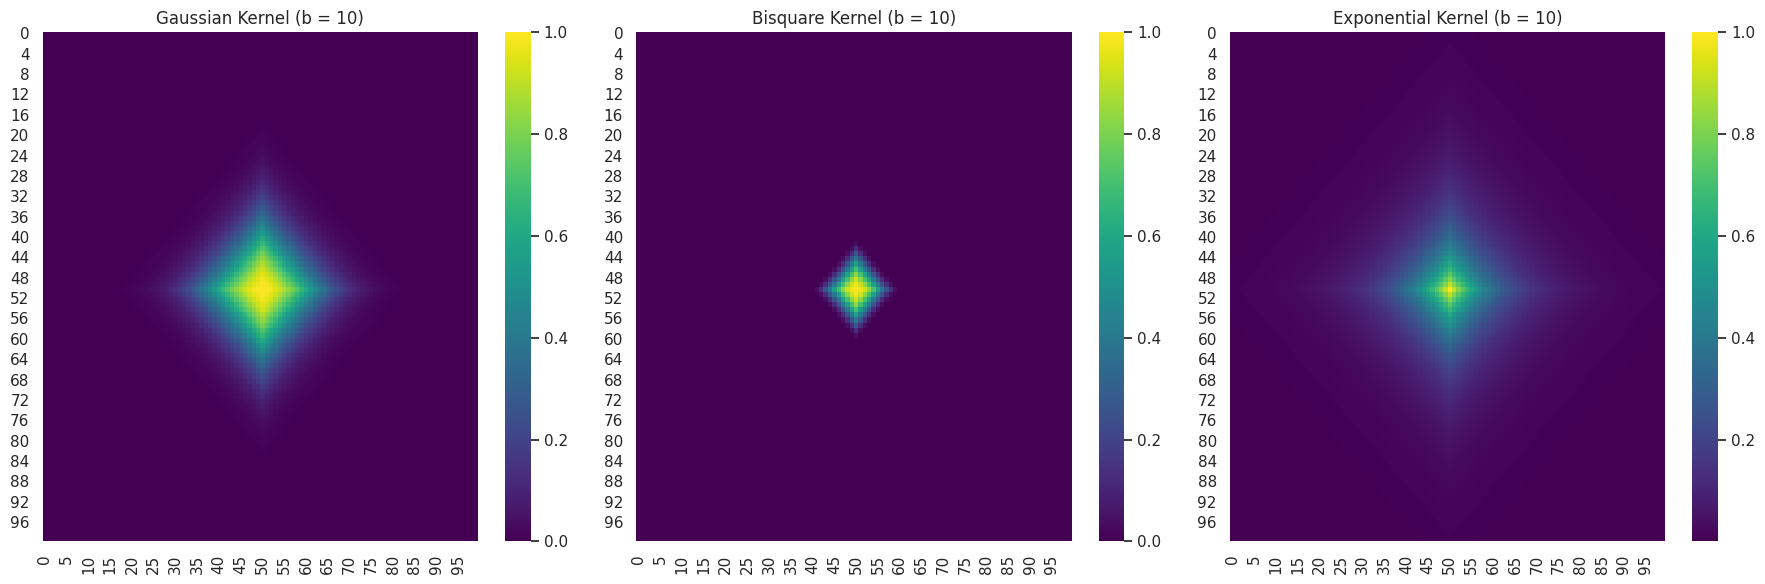
\includegraphics[width=0.85\linewidth]{gfx/m6l3_img001.png}
\par\smallskip{\small \textbf{Hình:} Hàm nhân (kernel) theo khoảng cách Manhattan, băng thông 10.}
\end{figure}

\begin{figure}[H]
\centering
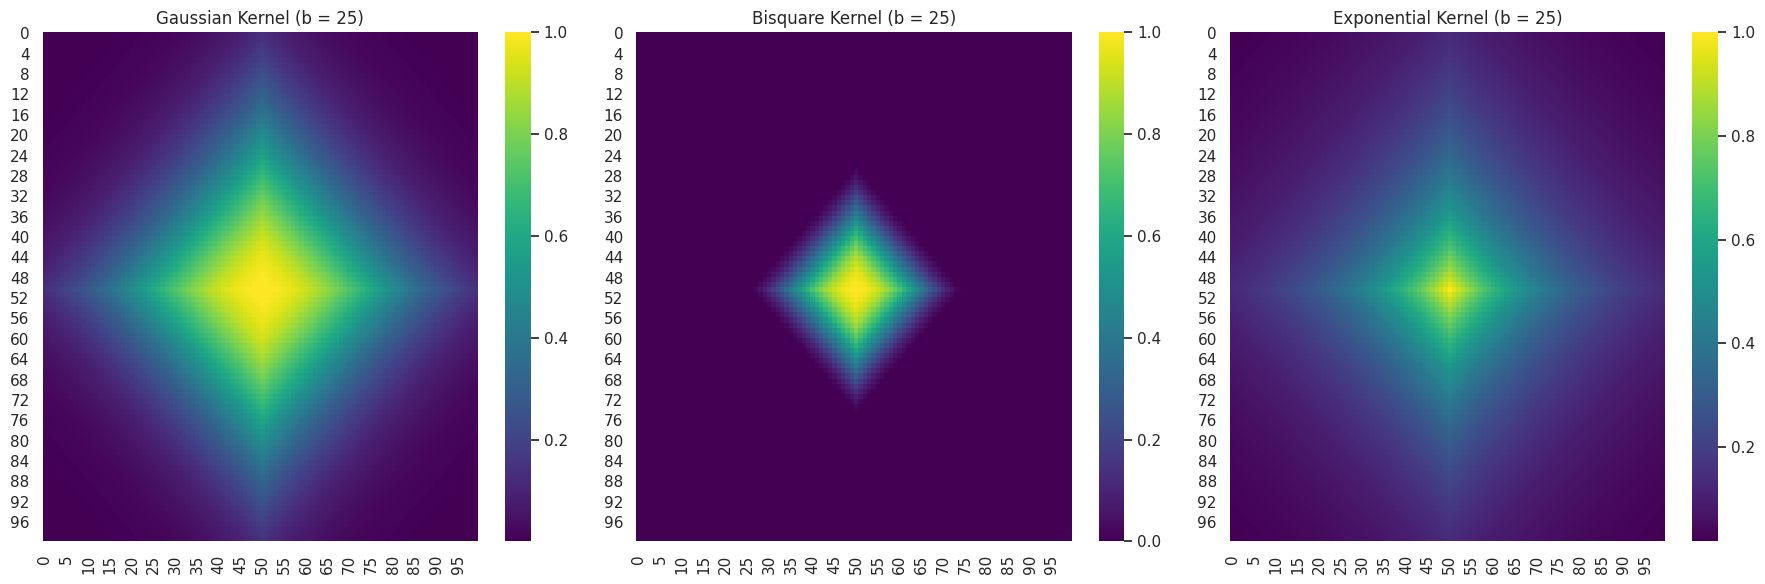
\includegraphics[width=0.85\linewidth]{gfx/m6l3_img002.png}
\par\smallskip{\small \textbf{Hình:} Hàm nhân (kernel) theo khoảng cách Manhattan, băng thông 25.}
\end{figure}

\begin{figure}[H]
\centering
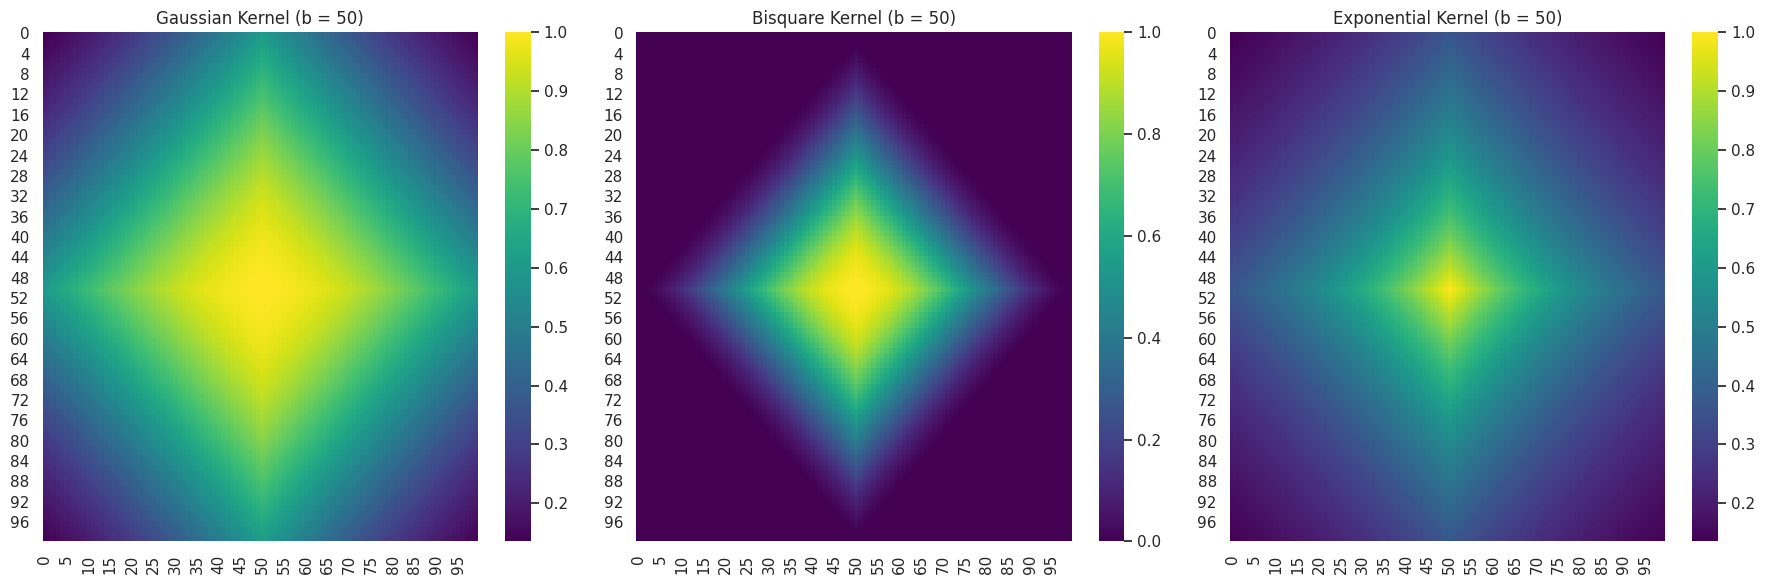
\includegraphics[width=0.85\linewidth]{gfx/m6l3_img003.png}
\par\smallskip{\small \textbf{Hình:} Hàm nhân (kernel) theo khoảng cách Manhattan, băng thông 50.}
\end{figure}

\begin{lstlisting}[language=Python,escapeinside={(*@}{@*)}]
# Figure 2
# Plot the kernels using Euclidean distance
for b in [10, 25, 50]:
    plot_kernels(D = euclidean_distance, bandwidth=b)
\end{lstlisting}

\begin{figure}[H]
\centering
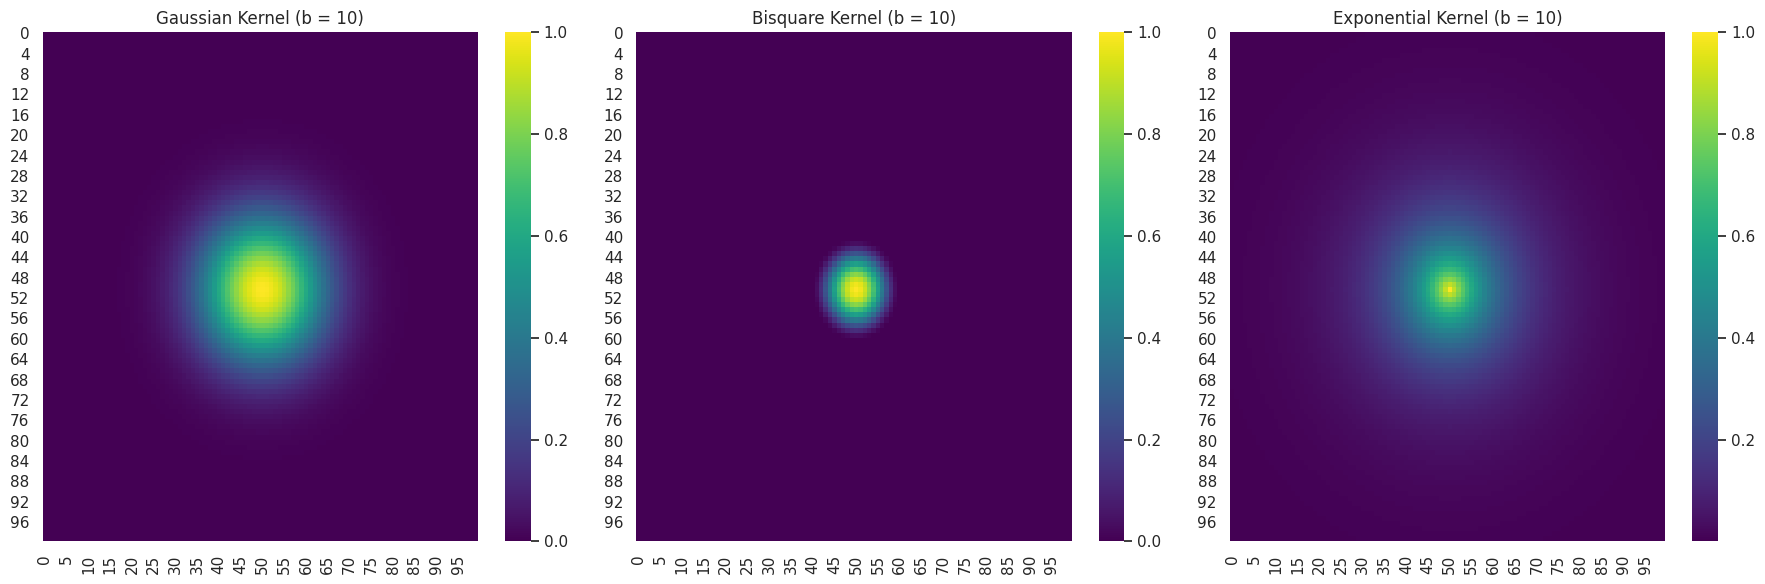
\includegraphics[width=0.85\linewidth]{gfx/m6l3_img004.png}
\par\smallskip{\small \textbf{Hình:} Hàm nhân (kernel) theo khoảng cách Euclid, băng thông 10.}
\end{figure}

\begin{figure}[H]
\centering
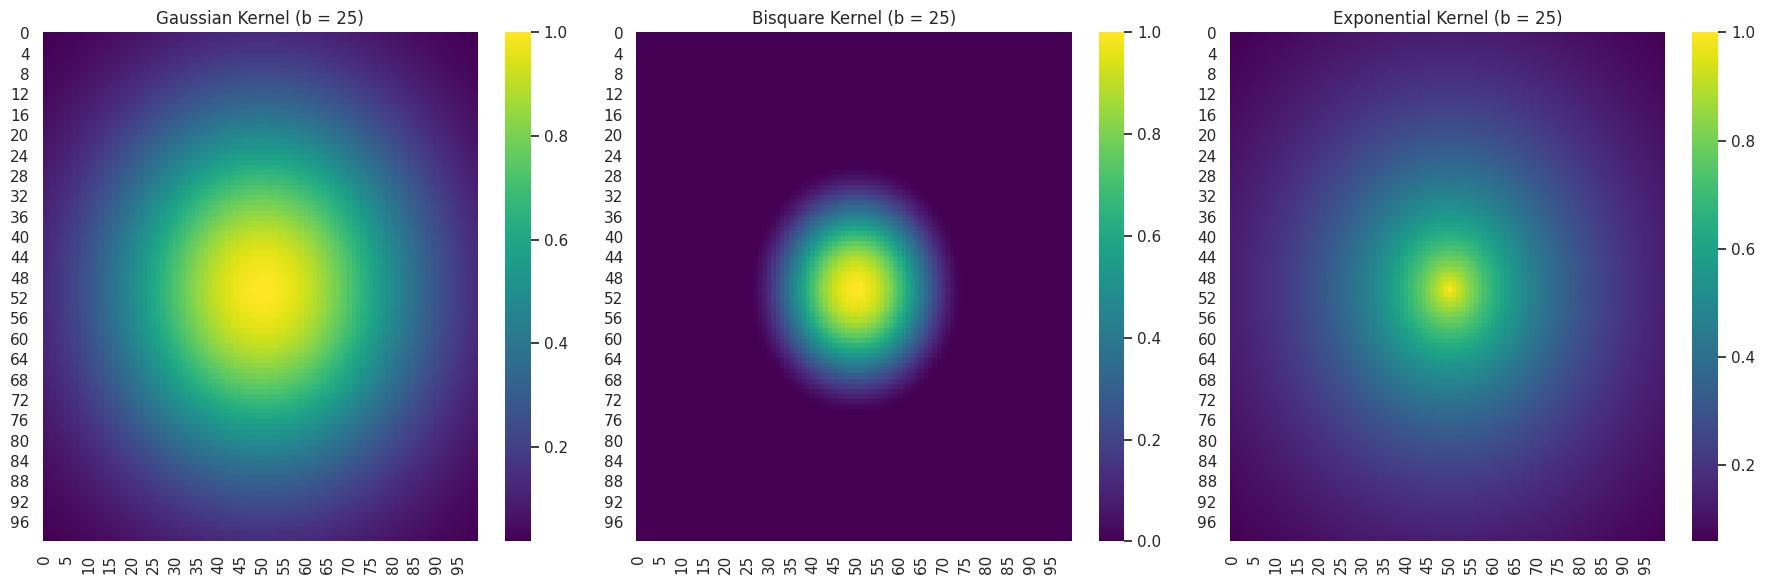
\includegraphics[width=0.85\linewidth]{gfx/m6l3_img005.png}
\par\smallskip{\small \textbf{Hình:} Hàm nhân (kernel) theo khoảng cách Euclid, băng thông 25.}
\end{figure}

\begin{figure}[H]
\centering
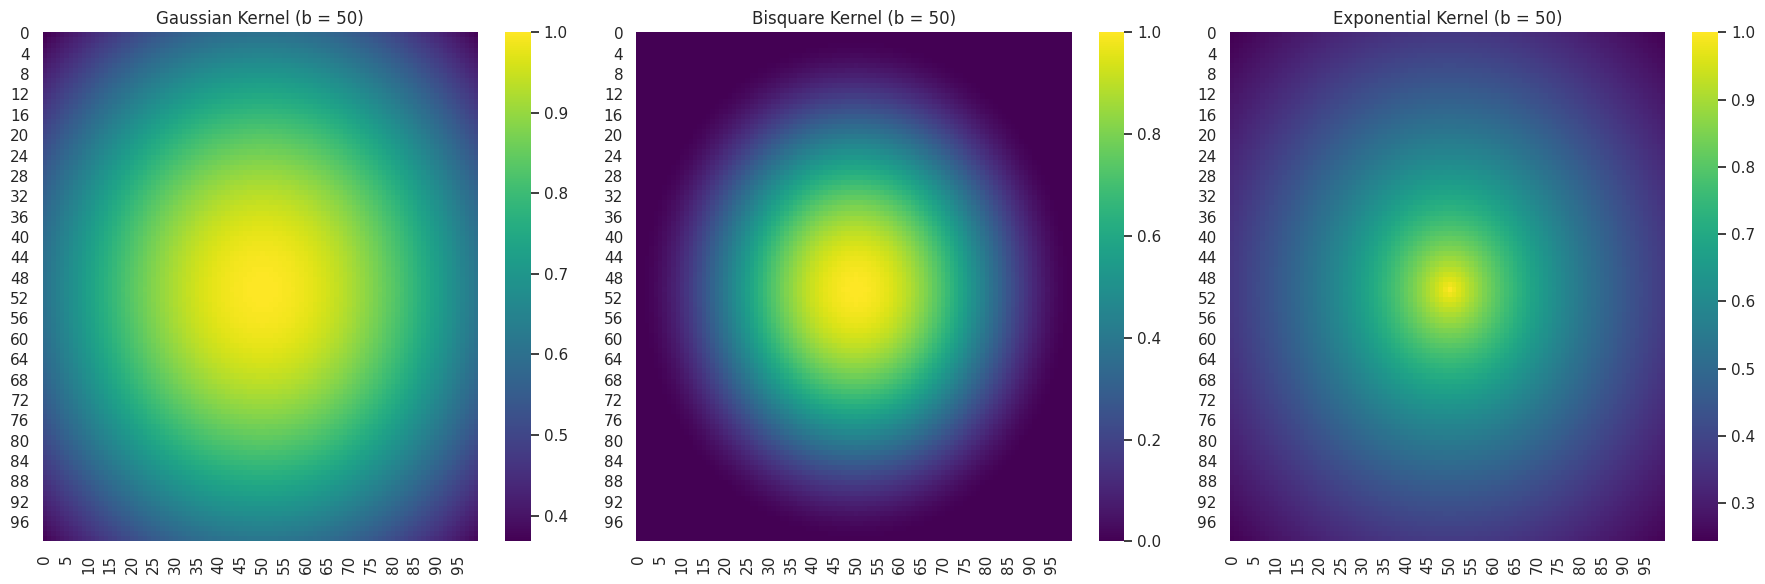
\includegraphics[width=0.85\linewidth]{gfx/m6l3_img006.png}
\par\smallskip{\small \textbf{Hình:} Hàm nhân (kernel) theo khoảng cách Euclid, băng thông 50.}
\end{figure}

Ở Hình 1 và 2, ta thấy tác động của băng thông lên việc chọn vùng lân cận: băng thông tăng thì vùng dùng trong hồi quy cục bộ cũng rộng ra. Hình dạng vùng cũng khác nhau theo từng thước đo khoảng cách. Quan trọng hơn, các hình làm rõ sự khác biệt giữa các hàm nhân:

\begin{itemize}
\item
  Gaussian: suy giảm dần và mượt, bắt đầu từ điểm quan tâm
\item
  Bisquare: cắt đột ngột, xác định rõ biên ảnh hưởng
\item
  Exponential: suy giảm nhanh nhưng có đuôi dài phản ánh các tác động ở khoảng cách xa
\end{itemize}

\section{Ứng dụng hồi quy trọng số địa lý (GWR)}

Trong phần này, chúng ta áp dụng những gì đã học về GWR ở phần trước vào dữ liệu thực tế.

\subsection{Nhập nguồn dữ liệu}

Ví dụ sử dụng dữ liệu cho thuê Airbnb tại khu Prenzlauer Berg (Prenz) ở Berlin, Đức (Oshan et al.). Prenz là điểm đến du lịch nổi tiếng, có nhiều lựa chọn ăn uống, nghệ thuật và đời sống về đêm. Dữ liệu được dùng để tìm hiểu các yếu tố chính quyết định giá thuê Airbnb trong khu vực này. Bộ dữ liệu có sẵn qua gói Python libpysal, nên cần cài gói này trước. Gói thứ hai cần cài là mgwr, gói Python để chạy GWR. Cài hai gói như sau.

\begin{lstlisting}[language=Python,escapeinside={(*@}{@*)}]
pip install libpysal
\end{lstlisting}

\begin{lstlisting}[language=Python,escapeinside={(*@}{@*)}]
pip install mgwr
\end{lstlisting}

Tiếp theo, nhập các gói Python cần thiết cho ứng dụng này.

\begin{lstlisting}[language=Python,escapeinside={(*@}{@*)}]
import pandas as pd
import libpysal as ps
from libpysal.examples import available
from libpysal.examples import load_example
from libpysal.examples import get_path
from mgwr.gwr import GWR, MGWR
from mgwr.sel_bw import Sel_BW
from mgwr.utils import compare_surfaces, truncate_colormap
import geopandas as gp
import folium
\end{lstlisting}

Pysal chứa nhiều bộ dữ liệu mẫu cho phân tích không gian; chi tiết xem tại \href{https://pysal.org/notebooks/lib/libpysal/Example_Datasets.html\#Datasets-for-use-with-libpysal}{Pysal Example Data}. Hàm sau cho phép xem danh sách các bộ dữ liệu mẫu của Pysal.

\begin{lstlisting}[language=Python,escapeinside={(*@}{@*)}]
# Check available datasets on Pysal
available()
\end{lstlisting}

Output:

\begin{lstlisting}[escapeinside={(*@}{@*)}]
         Name                                        Description  Installed
0       10740  Albuquerque, New Mexico, Census 2000 Tract Dat...       True
1      AirBnB  Airbnb rentals, socioeconomics, and crime in C...      False
2     Atlanta       Atlanta, GA region homicide counts and rates      False
3   Baltimore          Baltimore house sales prices and hedonics      False
4   Bostonhsg               Boston housing and neighborhood data      False
..        ...                                                ...        ...
94        taz           Traffic Analysis Zones in So. California      False
95      tokyo                               Tokyo Mortality data       True
96  us_income  Per-capita income for the lower 48 US states 1...       True
97   virginia                        Virginia counties shapefile       True
98       wmat          Datasets used for spatial weights testing       True

[99 rows x 3 columns]
\end{lstlisting}

Tiếp theo, tải bộ dữ liệu Prenz. Trên Pysal bộ này có tên "Berlin", nên đoạn mã dưới đây tải bộ dữ liệu Berlin.

\begin{lstlisting}[language=Python,escapeinside={(*@}{@*)}]
#Download Prenz (Berlin) dataset from Pysal
berlin = load_example('berlin')

# Check if the dataset is intalled and ready for analysis
berlin.installed
\end{lstlisting}

Output:

\begin{lstlisting}[escapeinside={(*@}{@*)}]
True
\end{lstlisting}

\subsection{Trực quan hóa dữ liệu}

Bộ dữ liệu đã được cài đặt. Hãy xem bên trong có gì.

\begin{lstlisting}[language=Python,escapeinside={(*@}{@*)}]
# Check file lists from the installed dataset
berlin.get_file_list()
\end{lstlisting}

Output:

\begin{lstlisting}[escapeinside={(*@}{@*)}]
['/usr/local/lib/python3.10/dist-packages/libpysal/examples/berlin/prenzlauer.zip',
 '/usr/local/lib/python3.10/dist-packages/libpysal/examples/berlin/README.md',
 '/usr/local/lib/python3.10/dist-packages/libpysal/examples/berlin/prenz_bound.zip']
\end{lstlisting}

Trong danh sách tệp, "prenzlauer.zip" chứa dữ liệu cần phân tích, còn "prenz\_bound.zip" dùng để vẽ ranh giới khu Prenz. Ta dùng hàm "get\_path" của Pysal và hàm "read.file" của geopandas để chuyển hai tệp này thành geo-dataframe.

\begin{lstlisting}[language=Python,escapeinside={(*@}{@*)}]
# Convert two zipped files to geo dataframes
prenz = gp.read_file(berlin.get_path('prenzlauer.zip'))
prenz_bound = gp.read_file(berlin.get_path('prenz_bound.zip'))
\end{lstlisting}

Kiểm tra lại kiểu của hai tệp đã chuyển đổi.

\begin{lstlisting}[language=Python,escapeinside={(*@}{@*)}]
# Check the type of Prenz dataset
type(prenz)
\end{lstlisting}

Output:

\begin{lstlisting}[escapeinside={(*@}{@*)}]
geopandas.geodataframe.GeoDataFrame
\end{lstlisting}

\begin{lstlisting}[language=Python,escapeinside={(*@}{@*)}]
# Check the type of Prenz_bound dataset
type(prenz)
\end{lstlisting}

Output:

\begin{lstlisting}[escapeinside={(*@}{@*)}]
geopandas.geodataframe.GeoDataFrame
\end{lstlisting}

Cả hai đều là bộ dữ liệu địa lý. Xem nội dung của chúng.

\begin{lstlisting}[language=Python,escapeinside={(*@}{@*)}]
prenz.head()
\end{lstlisting}

Output:

\begin{lstlisting}[escapeinside={(*@}{@*)}]
   accommodat  review_sco  bedrooms  bathrooms  beds  price             X  \
0           2       100.0       1.0        1.0   1.0   35.0  1.494450e+06   
1           2        90.0       1.0        1.0   1.0   23.0  1.494354e+06   
2           2        93.0       1.0        1.0   1.0   38.0  1.494406e+06   
3           2       100.0       1.0        1.0   1.0   50.0  1.494271e+06   
4           2       100.0       1.0        1.0   1.0   80.0  1.493982e+06   

              Y                         geometry  
0  6.899036e+06  POINT (1494450.105 6899036.141)  
1  6.899121e+06  POINT (1494353.555 6899120.594)  
2  6.898809e+06  POINT (1494405.897 6898808.518)  
3  6.898655e+06  POINT (1494270.517 6898655.223)  
4  6.899397e+06  POINT (1493982.078 6899397.385)
\end{lstlisting}

\begin{lstlisting}[language=Python,escapeinside={(*@}{@*)}]
# Find out number of rental properties in the dataset
len(prenz)
\end{lstlisting}

Output:

\begin{lstlisting}[escapeinside={(*@}{@*)}]
2203
\end{lstlisting}

Đoạn mã trên hiển thị năm dòng đầu của dữ liệu Prenz và cho biết bộ dữ liệu có 2.203 căn nhà cho thuê. Mô tả các biến:

\begin{itemize}
\item
  \textbf{accommodat}: Số khách tối đa căn nhà có thể tiếp nhận
\item
  \textbf{review\_sco}: Điểm đánh giá tích lũy từ khách gần nhất đã lưu trú
\item
  \textbf{bedrooms}: Số phòng ngủ
\item
  \textbf{bathrooms}: Số phòng tắm
\item
  \textbf{beds}: Số giường
\item
  \textbf{price}: Giá thuê
\item
  \textbf{X}: Vĩ độ của vị trí căn nhà
\item
  \textbf{Y}: Kinh độ của vị trí căn nhà
\item
  \textbf{geometry}: Vị trí địa lý của căn nhà
\end{itemize}

Bài trước đã nêu đặc điểm chính của bộ dữ liệu địa lý là có biến địa lý "geometry" cung cấp thông tin vị trí cho mỗi đặc trưng. Vì vị trí nhà cho thuê là dữ liệu điểm, ta chỉ có một cặp tọa độ gồm vĩ độ và kinh độ.

Tiếp theo, xem bộ dữ liệu địa lý prenz\_bound.

\begin{lstlisting}[language=Python,escapeinside={(*@}{@*)}]
prenz_bound.head()
\end{lstlisting}

Output:

\begin{lstlisting}[escapeinside={(*@}{@*)}]
       neighbourh                                           geometry
0  Helmholtzplatz  POLYGON ((1496989.669 6899662.266, 1497008.148...
\end{lstlisting}

Như đã giải thích, prenz\_bound cung cấp thông tin địa lý để vẽ ranh giới khu Prenz. Bộ dữ liệu này gồm tọa độ của nhiều điểm trên bản đồ; nối các điểm đó lại sẽ tạo thành một vùng (đa giác), nên prenz\_bound chỉ có một dòng dữ liệu.

Trước khi phân tích, hãy vẽ vị trí các căn nhà cho thuê lên bản đồ.

\begin{lstlisting}[language=Python,escapeinside={(*@}{@*)}]
# Draw Rental Properties of Prenz on a map

# First, create a basemap
map = folium.Map(location=[52.542986,13.427986], zoom_start=13.5, control_scale=True)

# Then add the Prenz neighborhood borders to the map
folium.GeoJson(prenz_bound).add_to(map)

# Then add the Airbnb rental locations to the map. We will use a red dot to represent the location of one airbnb rental.
folium.GeoJson(prenz,
               marker=folium.Circle(radius=10, fill_color="red", fill_opacity=0.4, color="red", weight=1)).add_to(map)

map
\end{lstlisting}

Output:

\begin{lstlisting}[escapeinside={(*@}{@*)}]
<folium.folium.Map at 0x7e6897fc5000>
\end{lstlisting}

\subsection{Chạy mô hình GWR}

Trong phần này, ta dùng dữ liệu Prenz để xây dựng mô hình định giá GWR bằng gói Python mgwr. Biến phụ thuộc là logarit của giá, nhằm hiệu chỉnh độ lệch (skewness) của dữ liệu giá. Ba biến độc lập là điểm đánh giá, số khách và số phòng tắm. Phương trình tuyến tính có dạng sau.

\textbf{log(price) = hệ số chặn + điểm đánh giá + số khách + số phòng tắm}

Ta cũng tạo một biến danh sách chứa thông tin của hai biến \(u\) và \(v\) đã mô tả ở phần 1.

\begin{lstlisting}[language=Python,escapeinside={(*@}{@*)}]
#Create variables for Berlin GWR pricing model
#Take the logarithm of the price variable to correct for skewing
b_y = np.log(prenz['price'].values.reshape((-1, 1)))
b_X = prenz[['review_sco','accommodat','bathrooms']].values
u = prenz['X']
v = prenz['Y']
b_coords = list(zip(u, v))
\end{lstlisting}

Sau khi tạo xong các biến cần cho mô hình, bước tiếp theo là xác định tham số băng thông (bandwidth).

Gói mgwr cung cấp hàm Sel\_BW để tìm băng thông tối ưu. Ta dùng quy trình tối ưu hóa và tiêu chí khớp mô hình mặc định của Sel\_BW. Mặc định là hàm nhân (kernel) bisquare và khoảng cách Euclid. Chọn kernel bisquare vì nó gán trọng số 0 cho các vị trí ở xa, trong khi kernel Gaussian và hàm mũ luôn gán trọng số khác 0 cho các vị trí ở xa.

Sau đó, Sel\_BW dùng phương pháp tìm kiếm mặc định dựa trên AIC hiệu chỉnh (AICc) để tìm băng thông tối ưu. \textbf{AIC hiệu chỉnh (AICc)} là một dạng AIC đặc biệt dùng cho phân tích không gian. AICc có thành phần phạt đối với băng thông nhỏ, vì băng thông nhỏ làm mô hình phức tạp hơn.

Bây giờ ta tìm băng thông cho mô hình.

\begin{lstlisting}[language=Python,escapeinside={(*@}{@*)}]
#Find bandwidth parameter
selector = Sel_BW(b_coords, b_y, b_X)
bw = selector.search()
print(bw)
\end{lstlisting}

Output:

\begin{lstlisting}[escapeinside={(*@}{@*)}]
192.0
\end{lstlisting}

Có băng thông rồi, ta dùng nó làm đầu vào để xây dựng mô hình GWR.

\begin{lstlisting}[language=Python,escapeinside={(*@}{@*)}]
# Build a GWR model and print out model summary
gwr_model = GWR(b_coords, b_y, b_X, bw)
gwr_results = gwr_model.fit()
gwr_results.summary()
\end{lstlisting}

Kết quả hồi quy toàn cục trong bản tóm tắt trên là kết quả mô hình OLS cho dữ liệu Prenz. Nó được dùng làm mô hình chuẩn so sánh (benchmark) với mô hình GWR. Kết quả OLS gồm phần tóm tắt mô hình thông thường mà ta đã quen thuộc.

\subsection{Xem xét kết quả mô hình}

Khối tiếp theo của phần tóm tắt là kết quả mô hình GWR, trước hết cho biết hàm nhân (kernel) bisquare và băng thông (bandwidth) 192 được chọn cho mô hình này, cùng nhiều thông tin chẩn đoán mô hình. Chẳng hạn, R\textsuperscript{2} hiệu chỉnh của mô hình OLS là 0,271 trong khi của mô hình GWR là 0,391; như vậy GWR phù hợp dữ liệu tốt hơn OLS.

Tiếp theo là kết quả ước lượng tham số. Trong mô hình GWR, mỗi vị trí có một bộ ước lượng tham số cho các biến độc lập; ở đây mỗi biến độc lập có 2.203 ước lượng tham số. Trong phần tóm tắt trên, X0 là hệ số chặn, X1 là điểm đánh giá, X2 là số khách được phục vụ, X3 là số phòng tắm. Vì vậy phần tóm tắt cho biết trung bình, độ lệch chuẩn, giá trị nhỏ nhất, trung vị và lớn nhất của các ước lượng tham số của từng biến độc lập. Để xem chi tiết, ta dùng mã Python sau, hiển thị bộ tham số ước lượng cho từng vị trí; dưới đây là năm vị trí đầu tiên.

\begin{lstlisting}[language=Python,escapeinside={(*@}{@*)}]
# Show estimated parameters for
gwr_results.params[0:5]
\end{lstlisting}

Output:

\begin{lstlisting}[escapeinside={(*@}{@*)}]
array([[ 3.30479996e+00,  1.61014298e-03,  2.06243405e-01,
        -2.67321919e-02],
       [ 3.43635569e+00, -4.51930353e-04,  1.95844944e-01,
         5.37474550e-02],
       [ 3.27912291e+00,  2.92768647e-03,  2.12363255e-01,
        -8.10919052e-02],
       [ 2.88779932e+00,  5.06056110e-03,  2.45744327e-01,
        4.65164479e-02],
       [ 2.89309002e+00,  3.06784769e-03,  1.67282256e-01,
         3.42487452e-01]])
\end{lstlisting}

GWR xây dựng một hồi quy cho mỗi vị trí nên mỗi vị trí cũng có R\textsuperscript{2} riêng. Dưới đây là R\textsuperscript{2} của 10 vị trí đầu tiên.

\begin{lstlisting}[language=Python,escapeinside={(*@}{@*)}]
gwr_results.localR2[0:10]
\end{lstlisting}

Output:

\begin{lstlisting}[escapeinside={(*@}{@*)}]
array([[0.39583113],
       [0.41660429],
       [0.35650484],
       [0.43641022],
       [0.44784271],
       [0.41771337],
       [0.42162229],
       [0.41387561],
       [0.36649332],
       [0.46269692]])
\end{lstlisting}

Ta cũng có thể vẽ biểu đồ R\textsuperscript{2} của mọi vị trí.

\begin{lstlisting}[language=Python,escapeinside={(*@}{@*)}]
#Show local model fit (R squared) for all locations
prenz['R2'] = gwr_results.localR2
prenz.plot('R2', legend = True)
ax = plt.gca()
ax.get_xaxis().set_visible(False)
ax.get_yaxis().set_visible(False)
plt.title("Local Model Fit")
plt.show()
\end{lstlisting}

\begin{figure}[H]
\centering
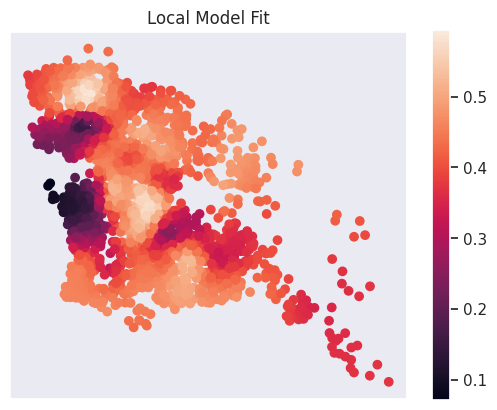
\includegraphics[width=0.85\linewidth]{gfx/m6l3_img007.png}
\par\smallskip{\small \textbf{Hình:} Độ khớp của mô hình cục bộ (Local Model Fit) trên bản đồ.}
\end{figure}

Từ biểu đồ "Local Model Fit", hai vùng sáng bên trái có nhiều vị trí nhất với R\textsuperscript{2} trên 0,5. Tuy nhiên, ở khu vực lệch trái so với trung tâm của khu phố, nhiều vị trí có R\textsuperscript{2} dưới 0,2.

\subsection{Minh họa tính các tham số GWR bằng đại số tuyến tính}

Phần này trình bày cách dùng đại số tuyến tính để thu được các ước lượng tham số của GWR. Trước hết, ta nhắc lại bộ ước lượng GWR cho các ước lượng tham số cục bộ tại vị trí \(i\).

\[\hat{\beta}(i)=\left[ X'W(i)X \right]^{-1}X'W(i)y\]

Ta dùng công thức trên để tính ước lượng tham số cho vị trí 1 (i bằng 0 vì Python đánh chỉ số từ 0). Vì ma trận trọng số được suy ra từ phương pháp tìm kiếm tối ưu, ta lấy trực tiếp từ kết quả mô hình để làm đầu vào.

\begin{lstlisting}[language=Python,escapeinside={(*@}{@*)}]
#Pull the information of weight matrix of location 1 from GWR model result
W_1 = gwr_results.W[0]
W_matrix = np.diag(W_1)
\end{lstlisting}

Tiếp theo, tạo ma trận \(X\): ma trận có các biến độc lập làm cột, kèm một cột toàn số 1 để ước lượng hệ số chặn.

\begin{lstlisting}[language=Python,escapeinside={(*@}{@*)}]
# Create X matrix with additional column of all 1s.
b_X_1 = np.hstack([np.ones((b_X.shape[0], 1)), b_X])
\end{lstlisting}

Tính trước ma trận nghịch đảo \(\left[ X'W(i)X \right]^{-1}\) trong công thức.

\begin{lstlisting}[language=Python,escapeinside={(*@}{@*)}]
inverse_matrix = np.linalg.inv(b_X_1.T@W_matrix@b_X_1)
\end{lstlisting}

Tiếp theo, tính ước lượng tham số cho vị trí 1.

\begin{lstlisting}[language=Python,escapeinside={(*@}{@*)}]
beta_1 = inverse_matrix@b_X_1.T@W_matrix@b_y
beta_1
\end{lstlisting}

Output:

\begin{lstlisting}[escapeinside={(*@}{@*)}]
array([[ 3.30479996e+00],
       [ 1.61014298e-03],
       [ 2.06243405e-01],
       [-2.67321919e-02]])
\end{lstlisting}

So sánh với kết quả của mô hình GWR.

\begin{lstlisting}[language=Python,escapeinside={(*@}{@*)}]
gwr_results.params[0]
\end{lstlisting}

Output:

\begin{lstlisting}[escapeinside={(*@}{@*)}]
array([ 3.30479996e+00,  1.61014298e-03,  2.06243405e-01, -2.67321919e-02])
\end{lstlisting}

Hai kết quả trùng khớp, cho thấy đại số tuyến tính được áp dụng thế nào vào việc tính mô hình GWR.

\section{Kết luận}

Bài học này trình bày lý thuyết về hồi quy trọng số địa lý (GWR), gồm định nghĩa và các khái niệm chính, đặc biệt là các phương pháp hàm nhân (kernel) và cách tính khoảng cách cho GWR, cũng như cách tính băng thông (bandwidth) của mô hình. Tiếp đó, chúng ta dùng một bộ dữ liệu thực tế để minh họa cách xây dựng mô hình GWR và so sánh kết quả với mô hình OLS truyền thống. Cuối cùng, chúng ta chỉ ra cách dùng đại số tuyến tính để suy ra các ước lượng tham số của mô hình GWR.

\chapter{Đọc thêm 1: Hồi quy trọng số địa lý (Brunsdon, Fotheringham \& Charlton)}
\label{ch:M6L3DocThem1}

\section{Thông tin nguồn}

\begin{itemize}
  \item \textbf{Nguồn:} Brunsdon, C., Fotheringham, A. S. \& Charlton, M. E. ``Geographically Weighted Regression: A Method for Exploring Spatial Nonstationarity.'' \emph{Geographical Analysis}, 28(4), 1996.
  \item \textbf{Phần cần đọc:} Toàn bộ bài báo (18 trang)
  \item \textbf{Ghi chú:} bản chuyển ngữ tiếng Việt súc tích, bám cấu trúc nguồn (giữ nguyên tiêu đề, công thức, số liệu, bảng, chú thích và danh mục tài liệu tham khảo).
\end{itemize}

Chris Brunsdon, A. Stewart Fotheringham và Martin E. Charlton

Hồi quy trọng số địa lý (Geographically Weighted Regression): Một phương pháp khám phá tính không dừng theo không gian

\textbf{Tóm tắt.} Tính không dừng theo không gian (spatial nonstationarity) là tình trạng một mô hình "toàn cục" đơn giản không thể giải thích quan hệ giữa một số tập biến; bản chất của mô hình phải thay đổi theo không gian để phản ánh cấu trúc trong dữ liệu. Bài báo phát triển một kỹ thuật gọi là hồi quy trọng số địa lý (GWR), hiệu chỉnh một mô hình hồi quy bội cho phép các quan hệ khác nhau tồn tại tại các điểm khác nhau trong không gian. Kỹ thuật này dựa lỏng lẻo trên hồi quy hàm nhân (kernel). Bài báo giới thiệu phương pháp và thảo luận các vấn đề liên quan như việc chọn hàm trọng số không gian. Tiếp theo là một loạt kiểm định thống kê nhằm kiểm tra tính không dừng theo không gian. Bằng phương pháp Monte Carlo, các tác giả đề xuất kỹ thuật kiểm định giả thuyết không rằng dữ liệu có thể được mô tả bằng một mô hình toàn cục thay vì mô hình không dừng, cũng như kiểm định xem từng hệ số hồi quy có ổn định trên không gian địa lý hay không. Các kỹ thuật được minh họa trên bộ dữ liệu điều tra dân số Anh năm 1991, liên hệ tỷ lệ sở hữu ô tô với tầng lớp xã hội và tỷ lệ thất nghiệp ở nam giới. Bài báo kết thúc bằng việc bàn về các hướng mở rộng kỹ thuật.

Một trong những mục tiêu chính của phân tích không gian là xác định bản chất các quan hệ giữa các biến, thường bằng cách tính thống kê hoặc ước lượng tham số từ quan sát tại các đơn vị không gian khác nhau trong vùng nghiên cứu. Các thống kê hay ước lượng tham số thu được thường được giả định là không đổi trên không gian, dù giả định này rất đáng ngờ trong nhiều trường hợp. Có thể quan hệ vốn khác nhau theo không gian, hoặc mô hình đo lường quan hệ bị đặc tả sai và điều đó biểu hiện thành các ước lượng tham số biến thiên theo không gian. Dù thế nào, một công cụ khám phá để mô tả và lập bản đồ các biến thiên không gian như vậy sẽ giúp hiểu rõ hơn các quan hệ đang nghiên cứu.

\emph{Chú thích tác giả: Chris Brunsdon là giảng viên về phương pháp dựa trên máy tính tại Khoa Quy hoạch Đô thị và Nông thôn; A. Stewart Fotheringham là Giáo sư Địa lý định lượng; Martin Charlton là giảng viên về GIS tại Khoa Địa lý; tất cả thuộc Đại học Newcastle.}

\emph{Geographical Analysis, Vol. 28, No. 4 (October 1996), Ohio State University Press. Nộp 6/7/95; bản sửa đổi được chấp nhận 2/16/96.}

Đã có một số kỹ thuật phục vụ mục đích này, nhưng các tác giả cho rằng phương pháp trong bài có nhiều ưu điểm quan trọng. Khung được biết đến nhiều nhất để đo "độ trôi" tham số là phương pháp mở rộng của Casetti (Casetti 1972; Casetti và Jones 1992), trong đó các tham số của mô hình toàn cục được làm thành hàm của không gian địa lý để đo xu hướng biến thiên tham số (xem Fotheringham và Pitts 1995; Eldridge và Jones 1991). Tuy quan trọng, đây chỉ là bài toán khớp xu hướng, ít hữu ích khi tham số biến thiên phức tạp trong không gian nghiên cứu. GWR cho phép ước lượng và lập bản đồ chính các tham số thực tại từng vị trí, thay vì khớp một mặt xu hướng lên chúng.

Phương pháp lọc thích nghi không gian (SAF) cũng từng được đề xuất để xử lý các quan hệ biến thiên theo không gian (Foster và Gorr 1986; Gorr và Olligschlaeger 1994). Tuy nhiên, cách này đưa quan hệ không gian vào theo kiểu ad hoc và cho ra các ước lượng tham số không thể kiểm định thống kê, nên phạm vi áp dụng hạn chế.

Hai phương pháp khác mô hình hóa biến thiên không gian của ước lượng tham số là mô hình hệ số ngẫu nhiên (Aitken 1996) và mô hình đa cấp (Goldstein 1987). Cả hai đều giả định các ước lượng tham số trong mô hình hồi quy là biến ngẫu nhiên: ở mô hình đa cấp, phân phối của chúng được giả định là Gauss, còn ở mô hình hệ số ngẫu nhiên, các tham số được mô hình hóa như phân phối hỗn hợp hữu hạn. Trong cả hai trường hợp, nhờ định lý Bayes có thể thu được ước lượng cho từng tham số, nhưng không có phụ thuộc không gian nào được giả định giữa các ước lượng, điều này không thực tế với mô hình các hiện tượng không gian. Dù các biến thể địa lý của mô hình đa cấp đã được áp dụng (Jones 1991), chúng phụ thuộc nhiều vào giả định về phân cấp các đơn vị không gian. Điều này có thể hợp lý nếu bản chất phân cấp được phản ánh tốt trong quá trình được mô hình hóa; còn trong các trường hợp khác, một mô hình liên kết không gian kiểu "suy giảm theo khoảng cách" như GWR có thể phù hợp hơn.

\section{2. TÍNH KHÔNG DỪNG THEO KHÔNG GIAN TRONG BỐI CẢNH HỒI QUY}

Mô hình thường dùng trong phân tích địa lý là hồi quy tuyến tính đơn giản (xem Dobson 1990, tr. 68-78). Trong kỹ thuật này, một biến (biến phụ thuộc) được mô hình hóa như hàm tuyến tính của một tập biến độc lập hay biến dự báo:

\begin{equation*}y_i = a_0 + \sum_{k=1}^{m} a_k x_{ik} + \varepsilon_i \tag{1}\end{equation*}

trong đó \(y_i\) là quan sát thứ \(i\) của biến phụ thuộc, \(x_{ik}\) là quan sát thứ \(i\) của biến độc lập thứ \(k\), các \(\varepsilon_i\) là các sai số độc lập phân phối chuẩn với trung bình bằng 0, và mỗi \(a_k\) phải được xác định từ mẫu gồm \(n\) quan sát. Thông thường dùng phương pháp bình phương tối thiểu để ước lượng các \(a_k\). Dùng ký hiệu ma trận, có thể viết:

\begin{equation*}\hat{\mathbf{a}} = (\mathbf{X}^T \mathbf{X})^{-1} \mathbf{X}^T \mathbf{y} \tag{2}\end{equation*}

trong đó các quan sát độc lập là các cột của x và các quan sát phụ thuộc là vectơ cột đơn y.* Vectơ cột chứa các ước lượng hệ số. Mỗi ước lượng có thể được hiểu là một "tốc độ thay đổi" giữa một biến độc lập và biến phụ thuộc. Chẳng hạn, nếu y là giá nhà đã thỏa thuận, còn x gồm nhiều biến liên quan đến thuộc tính của ngôi nhà và môi trường xung quanh, thì các hệ số có thể dùng để ước lượng mức thay đổi giá nhà khi có thêm một mét vuông sân vườn, thêm một phòng ngủ, hoặc khi nhà nằm gần trường học nhất hơn một kilômét.

Cần lưu ý rằng các tốc độ thay đổi này được giả định là phổ quát. Dù ngôi nhà nằm ở đâu, mức tăng giá biên khi có thêm một phòng ngủ vẫn cố định. Tuy nhiên, điều này có thể không đúng. Có thể hợp lý hơn khi giả định rằng tốc độ thay đổi do văn hóa và hiểu biết địa phương quyết định, thay vì một độ thỏa dụng toàn cục áp dụng cho mỗi hàng hóa. Quay lại ví dụ, giá trị gia tăng của một phòng ngủ thêm có thể lớn hơn ở khu dân cư đông gia đình có con, nơi không gian rộng thêm được xem là rất có lợi, so với khu dân cư của người độc thân hoặc các cặp vợ chồng cao tuổi, đối với họ không gian rộng thêm có thể bị coi là một đặc trưng tiêu cực.

Sự biến thiên của các mối quan hệ theo không gian như trên được gọi là tính không dừng theo không gian (spatial nonstationarity). Trong một bài báo gần đây, Fotheringham, Charlton và Brunsdon (1996) minh họa mức độ các ước lượng tham số hồi quy có thể biến thiên theo không gian. Trong ví dụ của họ, một cửa sổ 7 x 7 được đặt lên mọi ô của ma trận 50 x 38, theo cách sao cho cửa sổ nằm hoàn toàn trong vùng nghiên cứu. Tại mỗi vị trí đặt, dữ liệu trong cửa sổ được dùng để hiệu chỉnh một mô hình hồi quy, nhờ đó mỗi ô có một tập ước lượng tham số đi kèm. Các ước lượng tham số sau đó có thể được vẽ bản đồ để cho thấy mức độ biến thiên không gian của các mối quan hệ ước lượng. Kết quả cho thấy (a) các mối quan hệ có thể biến thiên đáng kể theo không gian và ước lượng "toàn cục" có thể che khuất những mối quan hệ địa lý đáng quan tâm, và (b) sự biến thiên theo không gian có thể phức tạp đến mức làm vô hiệu các bài tập khớp xu hướng đơn giản. Một ví dụ về loại bề mặt tham số mà Fotheringham, Charlton và Brunsdon (1996) mô tả được trình bày ở Hình 1, cho mối quan hệ giữa mật độ dân số và độ cao ở một phần đông bắc Scotland. Bề mặt này thể hiện các ước lượng tham số cục bộ thu được từ kỹ thuật hồi quy cửa sổ nêu trên, trong đó một mô hình hồi quy tuyến tính bội được hiệu chỉnh bằng cửa sổ 7 x 7. Bề mặt là một tập giá trị tham số phức tạp, dao động từ -1,26 đến 0,75. Ở một số khu vực nghiên cứu, mối quan hệ giữa mật độ dân số và độ cao âm có ý nghĩa, còn ở những khu vực khác thì dương có ý nghĩa. Mặc dù bề mặt tham số này có những "thung lũng" và "đồi" thú vị, nó rõ ràng quá phức tạp để biểu diễn bằng một xu hướng tuyến tính hay bậc hai đơn giản. Tuy vậy, nó cho những hiểu biết thú vị về cách mối quan hệ cụ thể này biến thiên theo không gian, có thể dùng để khám phá những khía cạnh của quan hệ giữa hai biến mà nếu không có thể sẽ không được nghiên cứu.

Dù phương pháp của Fotheringham, Charlton và Brunsdon (1996) dùng để tạo Hình 1 phục vụ mục đích khám phá hữu ích, nó mang tính ad hoc. Vì vậy, mục đích của bài báo này là mô tả một kỹ thuật thống kê chính thức, mà chúng tôi gọi là hồi quy trọng số địa lý (GWR), cho phép các biến thiên không gian phức tạp trong ước lượng tham số được xác định, vẽ bản đồ và mô hình hóa.

* Đối với số hạng hằng số, x phải chứa một cột gồm các số 1.

\textbf{HÌNH 1.} Bề mặt tham số độ cao (các khoảng giá trị tham số: từ -1,26 đến -0,92; -0,92 đến -0,59; -0,59 đến -0,25; -0,25 đến 0,08; 0,08 đến 0,41; 0,41 đến 0,75)

\section{3. HỒI QUY TRỌNG SỐ ĐỊA LÝ}

GWR là một kỹ thuật tương đối đơn giản mở rộng khung hồi quy truyền thống của phương trình (1) bằng cách cho phép các tốc độ thay đổi biến thiên cục bộ, sao cho các hệ số trong mô hình, thay vì là ước lượng toàn cục, đặc thù cho một vị trí i. Khi đó phương trình hồi quy là k=l,m

trong đó \(a_{ik}\) là giá trị của tham số thứ \(k\) tại vị trí \(i\). Lưu ý (1) là trường hợp đặc biệt của (3), khi mọi hàm đều là hằng số trên toàn không gian. Như sẽ trình bày dưới đây, điểm \(i\) tại đó các tham số được ước lượng hoàn toàn có thể khái quát hóa và không nhất thiết chỉ là những điểm có dữ liệu thu thập. Với GWR, ta dễ dàng tính ước lượng tham số cho các vị trí nằm giữa các điểm dữ liệu, nhờ đó có thể lập bản đồ chi tiết về sự biến thiên không gian của các mối quan hệ.

Mặc dù mô hình (3) có vẻ chỉ là phần mở rộng đơn giản của mô hình (1), việc hiệu chỉnh (3) gặp khó khăn vì các đại lượng chưa biết thực chất là những hàm ánh xạ không gian địa lý lên trục số thực, chứ không phải các số vô hướng như trong (1). Trong một tập dữ liệu điển hình, các mẫu của biến phụ thuộc và biến độc lập được lấy tại một tập điểm mẫu, và các tham số phải được ước lượng từ chúng. Trong mô hình truyền thống, các ước lượng này là hằng số với mọi \(i\), nhưng ở phương trình (3) thì rõ ràng không phải vậy.

Với mô hình (3), một cách trực giác hợp lý là dựa các ước lượng \(a_{ik}\) vào các quan sát tại những điểm mẫu gần \(i\). Nếu giả định các \(a_{ik}\) có mức độ trơn nhất định, ta có thể xấp xỉ hợp lý bằng cách xét quan hệ giữa các biến quan sát trong vùng gần \(i\) về mặt địa lý.

Với phương pháp bình phương tối thiểu có trọng số (weighted least squares) để hiệu chỉnh mô hình hồi quy, các quan sát khác nhau có thể được nhấn mạnh khác nhau khi sinh ra tham số ước lượng. Trong bình phương tối thiểu thông thường, các ước lượng hệ số cực tiểu hóa tổng bình phương chênh lệch giữa \(y_i\) dự đoán và thực tế. Trong bình phương tối thiểu có trọng số, một nhân tố trọng số \(w_i\) được áp dụng cho mỗi bình phương chênh lệch trước khi cực tiểu hóa, sao cho sai số của một số dự đoán bị phạt nặng hơn các dự đoán khác. Nếu \(\mathbf{W}\) là ma trận đường chéo của các \(w_i\), thì các hệ số ước lượng thỏa mãn

\[\hat{a} = (X^T W X)^{-1} X^T W y \quad (4)\]

Trong GWR, việc đặt trọng số cho quan sát theo mức độ gần \(i\) cho phép ước lượng \(a_{ik}\) thỏa tiêu chí "các điểm hiệu chỉnh ở gần" nêu trên.

Lưu ý rằng trong các mô hình hồi quy có trọng số thông thường, giá trị \(w_i\) là hằng số, nên chỉ cần một lần hiệu chỉnh để có tập ước lượng hệ số; nhưng ở đây \(w\) thay đổi theo \(i\), nên mỗi điểm trong vùng nghiên cứu có một lần hiệu chỉnh riêng. Khi đó, công thức ước lượng tham số có thể viết tổng quát hơn là

\[\hat{a}(i) = (X^T W(i) X)^{-1} X^T W(i) y \quad (5)\]

Phương pháp này có nét tương đồng với hồi quy kernel và ước lượng mật độ kernel (Parzen 1962; Cleveland 1979; Cleveland và Devlin 1988; Silverman 1986; Brunsdon 1991, 1995; Wand và Jones 1995, tr. 114-115). Trong hồi quy kernel, \(y\) được mô hình hóa như một hàm phi tuyến của \(x\) bằng hồi quy có trọng số, với trọng số của quan sát thứ \(i\) phụ thuộc vào mức gần nhau giữa \(x\) và \(x_i\), với mỗi \(i\), và bộ ước lượng là

\[\hat{f}(x) = (X^T W(x) X)^{-1} X^T W(x) y. \quad (6)\]

Khác biệt cốt yếu giữa hai phương pháp là: ở (6), hồi quy kernel, hệ thống trọng số phụ thuộc vào vị trí trong "không gian thuộc tính" (Openshaw 1993) của các biến độc lập, còn ở (5), GWR, nó phụ thuộc vào vị trí trong không gian địa lý. Đầu ra của (5) thường là tập ước lượng tham số cục bộ trong không gian \(x\), nên có thể mô hình hóa các quan hệ phi tuyến và không đơn điệu mạnh giữa \(y\) và \(x\). Tuy nhiên, đầu ra điển hình của (6) là tập ước lượng tham số có thể vẽ lên bản đồ địa lý để biểu diễn tính không dừng hay sự "trôi" tham số.

\subsection{3.1 Lựa chọn hàm trọng số không gian}

Đến đây, ta mới chỉ nêu rằng \(w(i)\) là một sơ đồ trọng số dựa trên mức gần của \(i\) với các vị trí lấy mẫu xung quanh \(i\), mà chưa nêu quan hệ tường minh. Phần này xét việc lựa chọn quan hệ đó. Trước hết, xét sơ đồ trọng số ngầm định của (2). Ở đây

\[w_{ij} = 1 \quad \forall i, j \quad (7)\]

trong đó \(j\) là một điểm cụ thể trong không gian có dữ liệu quan sát và \(i\) là điểm bất kỳ trong không gian cần ước lượng tham số. Nghĩa là trong mô hình toàn cục, mỗi quan sát có trọng số bằng một. Bước đầu hướng tới việc đặt trọng số theo vùng lân cận là loại khỏi quá trình hiệu chỉnh mô hình những quan sát cách vùng đó xa hơn một khoảng \(d\) nào đó. Điều này tương đương đặt trọng số của chúng bằng không, cho hàm trọng số

\[w_{ij} = 1 \text{ nếu } d_{ij} < d; \quad w_{ij} = 0 \text{ trong trường hợp còn lại.} \quad (8)\]

Hàm (8) cho phép tính toán hiệu quả, vì với mỗi điểm cần tính hệ số, chỉ một tập con (thường khá nhỏ) các điểm mẫu cần đưa vào mô hình hồi quy. Tuy nhiên, hàm trọng số không gian (8) gặp vấn đề gián đoạn. Khi \(i\) thay đổi trong vùng nghiên cứu, các hệ số hồi quy có thể biến đổi đột ngột mỗi khi một điểm mẫu đi vào hoặc ra khỏi vùng đệm tròn quanh \(i\), tức vùng xác định dữ liệu được đưa vào hiệu chỉnh cho vị trí \(i\). Dù các thay đổi đột ngột của tham số theo không gian có thể thực sự tồn tại, ở đây sự thay đổi của các ước lượng chỉ là hệ quả (artifact) của cách bố trí các điểm mẫu, chứ không phản ánh quá trình nền tảng của hiện tượng đang nghiên cứu. Một cách khắc phục là xác định \(w_{ij}\) như một hàm liên tục của \(d_{ij}\), khoảng cách giữa \(i\) và \(j\). Khi đó, từ (5) có thể thấy các ước lượng hệ số sẽ biến thiên liên tục theo \(i\). Một lựa chọn hiển nhiên là

\[w_{ij} = \exp(-\beta d_{ij}^2) \qquad (9)\]

sao cho nếu \(i\) là điểm có dữ liệu quan sát thì trọng số của dữ liệu đó bằng 1, còn trọng số của các dữ liệu khác giảm theo đường cong Gauss khi khoảng cách giữa \(i\) và \(j\) tăng. Trong trường hợp này, việc đưa dữ liệu vào quá trình hiệu chỉnh trở nên "phân đoạn". Chẳng hạn, khi hiệu chỉnh mô hình cho điểm \(i\), nếu \(w_{ij} = 0.5\) thì dữ liệu tại \(j\) chỉ đóng góp một nửa trọng số so với dữ liệu tại chính \(i\). Với dữ liệu ở rất xa \(i\), trọng số gần như bằng không, tức là loại bỏ thực chất các quan sát này khỏi việc ước lượng tham số tại vị trí \(i\).

Có thể dung hòa giữa (8) và (9), vừa có tính chất thuận lợi về tính toán là loại mọi điểm cách \(i\) quá một khoảng nhất định, vừa có tính chất thuận lợi về phân tích là tính liên tục. Một ví dụ là hàm bisquare:

\[w_{ij} = \left[1 - d_{ij}^2/d^2\right]^2 \ \text{ nếu } d_{ij} < d; \qquad w_{ij} = 0 \ \text{ nếu ngược lại.} \qquad (10)\]

Hàm này loại các điểm ngoài bán kính \(d\) nhưng làm thoải dần trọng số của các điểm bên trong bán kính, sao cho \(w_{ij}\) là hàm liên tục và khả vi một lần với mọi điểm cách \(i\) ít hơn \(d\) đơn vị.

Dù dùng hàm trọng số cụ thể nào, ý tưởng cốt lõi của GWR là với mỗi điểm \(i\) có một "đỉnh ảnh hưởng" quanh \(i\) tương ứng với hàm trọng số, sao cho các quan sát mẫu gần \(i\) có ảnh hưởng lớn hơn các quan sát ở xa trong việc ước lượng tham số của \(i\). Phương pháp cửa sổ trượt dùng để tạo Hình 1 và được mô tả đầy đủ hơn ở nơi khác (Fotheringham, Charlton, and Brunsdon 1996) sử dụng hàm trọng số bằng 1 nếu các điểm \(i\) và \(j\) nằm trong hình vuông có các đỉnh \((-d/2,-d/2)\), \((-d/2,d/2)\), \((d/2,d/2)\) và \((d/2,-d/2)\), và bằng 0 trong các trường hợp còn lại. Về bản chất đây là hàm nhân (kernel) "cắt đột ngột" như (8), nhưng có dạng vuông thay vì tròn. Nhìn lại, đây là lựa chọn kernel khá kỳ quặc, mặc dù về tính toán thì nó phù hợp với khung raster.

\subsection{3.2 Hiệu chỉnh hàm trọng số}

Một khó khăn của GWR là các tham số ước lượng phần nào phụ thuộc vào hàm trọng số hay hàm nhân (kernel) được chọn. Chẳng hạn trong (8), khi \(d\) càng lớn thì nghiệm của mô hình càng gần với OLS, và khi \(d\) bằng khoảng cách lớn nhất giữa các điểm trong hệ thống thì hai mô hình trùng nhau. Tương tự, trong (9), khi \(\beta\) tiến về 0, trọng số tiến về 1 với mọi cặp điểm, nên các tham số ước lượng trở nên đồng nhất và GWR tương đương OLS. Ngược lại, khi độ suy giảm theo khoảng cách (distance-decay) càng lớn, các ước lượng tham số càng phụ thuộc vào các quan sát ở gần \(i\) và do đó có phương sai tăng. Vấn đề là làm thế nào chọn hàm suy giảm phù hợp trong GWR.

Xét việc chọn \(\beta\) trong (9). Một khả năng là chọn \(\beta\) theo tiêu chí bình phương tối thiểu. Nếu các sai số trong (3) được giả định là Gauss thì điều này cũng thỏa tiêu chí hợp lý cực đại. Rõ ràng cách làm là cực tiểu hóa đại lượng

\[\sum_{i=1}^{n} \left[y_i - \hat{y}_i(\beta)\right]^2 \qquad (11)\]

trong đó \(\hat{y}_i(\beta)\) là giá trị khớp của \(y_i\) khi dùng độ suy giảm theo khoảng cách \(\beta\). Để tìm giá trị khớp của \(y_i\), cần ước lượng các \(a_{ik}\) tại mỗi điểm mẫu rồi kết hợp chúng với các giá trị \(z\) tại các điểm đó. Tuy nhiên, khi cực tiểu hóa tổng bình phương sai số như trên thì gặp một vấn đề. Giả sử \(\beta\) rất lớn sao cho trọng số của mọi điểm trừ chính \(i\) là không đáng kể. Khi đó các giá trị khớp tại các điểm mẫu sẽ tiến về giá trị thực, nên (11) bằng không. Điều này gợi ý rằng với tiêu chí tối ưu như vậy, \(\beta\) tiến tới vô cùng, nhưng rõ ràng trường hợp suy biến này vô ích. Thứ nhất, các tham số của mô hình như vậy không xác định trong trường hợp giới hạn này; thứ hai, các ước lượng sẽ dao động dữ dội trong không gian để cho giá trị khớp tốt cục bộ tại mỗi \(i\).

Giải pháp cho vấn đề này là phương pháp kiểm định chéo (cross-validation, CV) do Cleveland (1979) đề xuất cho hồi quy cục bộ và Bowman (1984) cho ước lượng mật độ kernel. Ở đây, ta dùng điểm số có dạng

\[CV = \sum_{i=1}^{n} \left[y_i - \hat{y}_{\neq i}(\beta)\right]^2 \qquad (12)\]

trong đó \(\hat{y}_{\neq i}(\beta)\) là giá trị khớp của \(y_i\) khi các quan sát tại điểm \(i\) bị bỏ ra khỏi quá trình hiệu chỉnh. Cách tiếp cận này có tính chất thuận lợi là chống được hiệu ứng quấn vòng (wrap-around), vì khi \(\beta\) rất lớn, mô hình chỉ được hiệu chỉnh trên các mẫu gần \(i\) chứ không phải tại chính \(i\).

Do đó, việc vẽ đồ thị điểm CV theo tham số cần thiết của hàm trọng số được chọn sẽ giúp định hướng chọn giá trị phù hợp cho tham số đó. Nếu muốn tự động hóa quy trình này, có thể cực đại hóa điểm CV bằng một kỹ thuật tối ưu hóa như tìm kiếm theo tỉ lệ vàng (Golden Section search; Greig 1980).

\subsection{3.3 Kiểm định tính không dừng theo không gian}

Cho đến đây, các kỹ thuật của GWR chủ yếu mang tính mô tả. Tuy nhiên, có hai câu hỏi hữu ích có thể được xem xét:

\begin{itemize}
\item
  Mô hình GWR có mô tả dữ liệu tốt hơn một cách có ý nghĩa thống kê so với mô hình hồi quy toàn cục hay không?
\item
  Tập các tham số \(a_{ik}\) có biến thiên không gian đáng kể hay không?
\end{itemize}

Ở câu hỏi thứ nhất, toàn bộ mô hình hồi quy thay đổi theo địa lý được đem ra kiểm định. Ở câu hỏi thứ hai, ta có thể kiểm định xem tốc độ thay đổi của một biến cụ thể có biến động đáng kể trên toàn vùng nghiên cứu hay không. Để trả lời cả hai câu hỏi, cần định nghĩa các thống kê mô tả cho mẫu. Trước hết, thống kê này mô tả mức độ "toàn cục" của mô hình. Một lựa chọn khả dĩ là tham số trọng số \(\beta\) thu được từ thủ tục CV, dùng để đánh giá mức khác biệt giữa mô hình GWR và mô hình toàn cục. Như đã nêu, giá trị \(\beta\) trong hàm mũ tiến về 0 đối với mô hình toàn cục, và độ lệch của ước lượng \(\hat{\beta}\) khỏi 0 cho biết mức độ khác biệt giữa mô hình cục bộ và mô hình toàn cục.

Đối với giả thuyết thứ hai, chính độ biến thiên của \(a_k\) có thể dùng để mô tả mức độ hợp lý của một hệ số không đổi. Nói chung, đây có thể xem như một thước đo phương sai. Với một \(k\) cho trước, giả sử \(\hat{a}_{ik}\) là ước lượng GWR của \(a_{ik}\). Khi đó, một ước lượng khả dĩ của độ biến thiên là "độ gồ ghề" (roughness) của \(a_k\), được định nghĩa là

(công thức gốc bị vỡ khi trích PDF; các thành phần: \(\int_G (\cdot)^2\,dx\,dy\) với \(G\) là vùng nghiên cứu)

trong đó \(G\) là vùng nghiên cứu. Đại lượng này có thể được ước lượng nếu xây dựng được một xấp xỉ dạng lưới cho \(a_{ik}\). Tuy nhiên, thống kê này khá cồng kềnh khi tính toán, nên ở đây đề xuất một phương án thay thế. Giả sử với mỗi điểm trong \(n\) điểm mẫu \(i\), ta tính được ước lượng tham số \(\hat{a}_{ik}\). Khi đó ta có \(n\) ước lượng của hệ số đang nghiên cứu. Một cách tiếp cận là tính độ lệch chuẩn của các giá trị này, cho ra ước lượng mẫu của (13). Thống kê này được gọi là \(s_k\).

Như vậy đã có hai loại thống kê, mỗi loại tương ứng với một câu hỏi nêu trên. Bước tiếp theo là xác định phân phối mẫu của chúng dưới giả thuyết không rằng mô hình (1) đúng. Dù trong tương lai sẽ xem xét các tính chất lý thuyết của các phân phối này, hiện tại sẽ áp dụng phương pháp Monte Carlo. Dưới giả thuyết không, mọi hoán vị của các cặp \((x_i, y_i)\) giữa các điểm lấy mẫu địa lý \(i\) đều có khả năng xảy ra như nhau. Do đó, các giá trị quan sát được của \(\beta\) hoặc \(s_k\) có thể được so sánh với các phân phối ngẫu nhiên hóa này để thực hiện kiểm định ý nghĩa thống kê. Với phương pháp Monte Carlo, việc chọn \(N\) hoán vị ngẫu nhiên của các cặp \((x_i, y_i)\) giữa các điểm \(i\) và tính \(\hat{\beta}\) hoặc \(s_k\) cũng cho một kiểm định ý nghĩa khi so với các thống kê quan sát được.

\textbf{Bảng 1.} Các biến dùng trong ví dụ GWR

{\small
\begin{longtable}[]{@{}
  >{\raggedright\arraybackslash}p{(\columnwidth - 6\tabcolsep) * \real{0.2222}}
  >{\raggedright\arraybackslash}p{(\columnwidth - 6\tabcolsep) * \real{0.2593}}
  >{\raggedright\arraybackslash}p{(\columnwidth - 6\tabcolsep) * \real{0.2963}}
  >{\raggedright\arraybackslash}p{(\columnwidth - 6\tabcolsep) * \real{0.2222}}@{}}
\toprule\noalign{}
\begin{minipage}[b]{\linewidth}\raggedright
Biến
\end{minipage} & \begin{minipage}[b]{\linewidth}\raggedright
Tử số
\end{minipage} & \begin{minipage}[b]{\linewidth}\raggedright
Mẫu số
\end{minipage} & \begin{minipage}[b]{\linewidth}\raggedright
Phụ thuộc (D) hoặc độc lập (I)
\end{minipage} \\
\midrule\noalign{}
\endhead
\bottomrule\noalign{}
\endlastfoot
Thất nghiệp nam & Dân số nam đang tìm việc & Dân số hoạt động kinh tế & I \\
Tầng lớp xã hội I & Số hộ có chủ hộ thuộc tầng lớp xã hội I & Tổng số hộ & I \\
Số xe trên mỗi hộ & Số xe & Số hộ (đơn vị trăm) & D \\
\end{longtable}
}

Khi thực hiện kiểm định cho \(\hat{\beta}\), lưu ý rằng chi phí tính toán có thể rất lớn: với mỗi hoán vị, phải tìm \(\beta\) tối ưu theo CV bằng tìm kiếm theo tỉ lệ vàng. Dù phương pháp này tốn thời gian, việc tính từng thống kê \(s_k\) cho mỗi hoán vị lại khá đơn giản sau khi \(\beta\) đã được hiệu chỉnh. Một cách tiết kiệm thời gian, nếu không cần kiểm định ý nghĩa của \(\beta\), là tối ưu \(\hat{\beta}\) từ dữ liệu quan sát rồi dùng giá trị này để thực hiện các ước lượng \(s_k\) còn lại dựa trên hoán vị.

\section{4. NGHIÊN CỨU TÌNH HUỐNG: SỞ HỮU Ô TÔ TẠI TYNE AND WEAR}

Trong phần này, kỹ thuật GWR được áp dụng cho dữ liệu điều tra dân số năm 1991 cấp phường (ward) của hạt Tyne and Wear, Vương quốc Anh. Hạt này có trung tâm là thành phố Newcastle và sông Tyne ở đông bắc nước Anh. Các mối quan hệ được khảo sát là giữa tỷ lệ sở hữu ô tô (biến phụ thuộc) và hai biến độc lập kinh tế - xã hội: tỷ lệ thất nghiệp nam giới và tỷ lệ hộ gia đình thuộc tầng lớp xã hội I (một biến điều tra dân số của Anh đo tỷ lệ hộ có chủ hộ làm nghề chuyên môn hoặc quản lý, thường được dùng làm biến đại diện cho các hộ thu nhập cao). Chi tiết về các biến này có trong Bảng 1 và phân bố không gian của chúng được vẽ ở Hình 2-4. Phân bố không gian của số ô tô trên mỗi hộ cho thấy các phường dọc sông Tyne, về phía trung tâm vùng, nhìn chung có số ô tô trên mỗi hộ thấp hơn các khu ngoại ô ở ngoại vi. Tỷ lệ thất nghiệp nam giới cao tập trung ở các phường trung tâm của Newcastle (ở gần giữa vùng) và Sunderland (ở phía đông nam). Phân bố của biến tầng lớp xã hội ít rõ nét hơn nhưng phản ánh các khu giàu có ở phía bắc Newcastle và một số khu ven biển ở phía đông của vùng.

Giả thuyết đặt ra là khi tỷ lệ thất nghiệp nam giới trong một phường tăng lên thì tỷ lệ sở hữu ô tô giảm, ceteris paribus (các yếu tố khác không đổi), và khi tỷ lệ hộ thuộc tầng lớp xã hội I tăng lên thì tỷ lệ sở hữu ô tô tăng, ceteris paribus. Các giả thuyết này được ủng hộ mạnh bởi kết quả hồi quy OLS toàn cục ở Bảng 2, trong đó cả hai ước lượng tham số đều khác 0 có ý nghĩa ở mức 99 phần trăm và đều có dấu như kỳ vọng. Giá trị R bình phương của mô hình là 0,83, cho thấy độ khớp cao với dữ liệu. Tuy nhiên, kết quả này không cho biết tính ổn định của các mối quan hệ trên toàn vùng nghiên cứu, và để làm điều đó cần áp dụng GWR.

FIG.2. Bản đồ số ô tô trên một trăm hộ theo phường (các mức: dưới 40; 40-55; 55-65; 65-75; trên 75)

FIG.3. Bản đồ tỷ lệ thất nghiệp nam giới theo phường (các mức: dưới 10\%; 10\%-15\%; 15\%-20\%; 20\%-25\%; trên 25\%)

\subsection{4.1 Ứng dụng GWR}

Vì GWR là kỹ thuật dựa trên các điểm mẫu, các biến gắn với mỗi phường được giả định là mẫu lấy tại tâm (centroid) của phường đó, sao cho điểm i được xác định là tâm của phường i. Theo cách này, hiệu ứng suy giảm theo khoảng cách vẫn được áp dụng, với ảnh hưởng của mỗi phường lên ước lượng a\_ik giảm dần khi khoảng cách từ tâm phường đến i tăng. Điều này cũng cung cấp một cách hữu ích để lập bản đồ kết quả phân tích: nếu a\_ik được ước lượng cho từng tâm phường và giá trị đó được gán cho phường tương ứng thì có thể vẽ bản đồ choropleth về sự biến thiên của các hệ số. Các giá trị hệ số này cũng có thể làm cơ sở cho các kiểm định ý nghĩa đã mô tả ở trên.

FIG.4. Bản đồ tỷ lệ chủ hộ thuộc tầng lớp xã hội I theo phường (các mức: dưới 1\%; 1\%-2\%; 2\%-3\%; 3\%-4\%; trên 4\%)

\textbf{BẢNG 2} Kết quả hồi quy OLS toàn cục

{\small
\begin{longtable}[]{@{}llll@{}}
\toprule\noalign{}
Tham số & Giá trị ước lượng & Sai số chuẩn & Giá trị t \\
\midrule\noalign{}
\endhead
\bottomrule\noalign{}
\endlastfoot
Hệ số chặn (Intercept) & 88,5 & 2,89 & 30,6 \\
Tầng lớp xã hội & 1,88 & 0,33 & 5,7 \\
Thất nghiệp & -1,83 & 0,11 & 16,6 \\
\end{longtable}
}

R² = 0,83

Các mô hình GWR với hàm trọng số không gian mô tả ở (9) và nhiều giá trị \ensuremath{\beta} khác nhau được áp dụng cho dữ liệu mô tả ở Bảng 1 và Hình 2-4. Giá trị tổng bình phương sai số kiểm định chéo (CVSS) được vẽ theo hàm của \ensuremath{\beta} ở Hình 5. Từ đó thấy có một giá trị \ensuremath{\beta} tối ưu toàn cục quanh 0,303, được xác nhận bằng thuật toán tối ưu Golden Section. Tại giá trị này, điểm CV xấp xỉ một nửa so với trường hợp hồi quy toàn cục (\ensuremath{\beta} = 0). Sơ đồ trọng số quanh một phường ở trung tâm thành phố ứng với \ensuremath{\beta} tối ưu được minh họa ở Hình 6. Mẫu này cho thấy dữ liệu được gán trọng số theo không gian như thế nào để ước lượng tham số cho phường đó. Sơ đồ trọng số được đặt tâm tại từng phường để ước lượng các tham số biến thiên theo không gian.

FIG.5. Hiệu chỉnh hàm trọng số không gian

FIG.6. Bản đồ hàm trọng số theo phường (các mức: dưới 0,01; 0,01-0,03; 0,03-0,06; 0,06-0,30; 0,30-1,00)

Kết quả chính của GWR, tức sự biến thiên không gian của các ước lượng tham số, được thể hiện ở Hình 7-9 lần lượt cho hệ số chặn, tầng lớp xã hội và thất nghiệp. Sự biến thiên không gian của các mối quan hệ được bộc lộ bởi

Các phân bố này đáng chú ý. Chẳng hạn, các số hạng chặn (intercept) cho thấy một mô hình không gian rõ rệt, với giá trị cao hơn ở phía tây bắc và đông nam của vùng. Đây là những khu vực ít đô thị hóa hơn, và gợi ý rằng, với các điều kiện khác không đổi (ceteris paribus), tỷ lệ sở hữu ô tô cao hơn gắn với các khu vực nông thôn hơn. Điều này có thể liên quan đến mức độ giao thông công cộng thấp hơn và khả năng tiếp cận dịch vụ kém hơn ở các khu vực đó. Mối quan hệ giữa tỷ lệ sở hữu ô tô và tầng lớp xã hội ở Hình 8 cho thấy, với các điều kiện khác không đổi và cùng một tỷ lệ hộ gia đình thuộc tầng lớp xã hội I, tỷ lệ sở hữu ô tô cao hơn ở các phường hướng ra bờ biển và trong một dải gần rìa phía nam của vùng. Một cách giải thích khả dĩ là tỷ lệ sở hữu ô tô cao hơn ở các phường giàu hơn nhưng không được phục vụ tốt bởi hệ thống giao thông công cộng đường sắt nhẹ của vùng, vốn tập trung vào thành phố Newcastle, xấp xỉ ở trung tâm khu vực nghiên cứu. Phân bố của tham số thất nghiệp cho thấy mối quan hệ này ít âm hơn trong lõi đô thị hóa cao của khu vực nghiên cứu và trong một dải chạy từ tây nam sang đông bắc qua phần phía nam của vùng. Nguyên nhân chưa rõ ràng ngay lập tức. Một ứng dụng quan trọng của GWR là làm công cụ khám phá để điều tra thêm các câu hỏi và phát hiện mà nếu không có thể bị bỏ sót.

\textbf{HÌNH 7.} Bản đồ hệ số chặn (intercept) theo phường (các mức: dưới 75; 75-80; 80-85; 85-90; trên 90).

\textbf{HÌNH 8.} Bản đồ hệ số Tầng lớp xã hội I theo phường (các mức: dưới 0; 0,0-1,5; 1,5-3,0; 3,0-4,5; trên 4,5).

\textbf{HÌNH 9.} Bản đồ hệ số Thất nghiệp nam theo phường (các mức: dưới -1,7; -1,7 đến -1,6; -1,6 đến -1,5; -1,5 đến -1,4; trên -1,4).

\textbf{BẢNG 3} Kiểm định ý nghĩa thống kê cho tính không dừng

{\small
\begin{longtable}[]{@{}lll@{}}
\toprule\noalign{}
Biến & \(s_i\) & giá trị p \\
\midrule\noalign{}
\endhead
\bottomrule\noalign{}
\endlastfoot
Intercept (hệ số chặn) & 6.34 & 0.40 \\
Tầng lớp xã hội I & 1.66 & 0.04 \\
Thất nghiệp nam & 0.17 & 0.96 \\
\end{longtable}
}

Trước khi bàn chi tiết hơn về các kết quả này, cần đánh giá ý nghĩa thống kê của các biến thiên không gian trong các ước lượng tham số, được xác định bằng cách tính các thống kê \(s_i\) theo phương pháp Monte Carlo đã mô tả ở trên. Kết quả các kiểm định được trình bày ở Bảng 3.

Từ đó có thể thấy hệ số duy nhất biến thiên có ý nghĩa theo không gian là hệ số gắn với tỷ lệ tầng lớp xã hội I trong một phường. Điều này cũng được củng cố bởi việc độ lệch chuẩn của các ước lượng tham số biến thiên theo không gian của biến này (1,66) lớn hơn năm lần sai số chuẩn của ước lượng tham số toàn cục (0,33, như trong Bảng 2). Một cách diễn giải khả dĩ là: dù người thất nghiệp có thể coi trọng khả năng tiếp cận giao thông ở nông thôn hơn ở thành thị, thực tế cho thấy việc duy trì một chiếc ô tô có thể quá tốn kém, nên mức thất nghiệp không ảnh hưởng đến tỷ lệ sở hữu ô tô theo cách khác nhau giữa nông thôn và thành thị. Tuy nhiên, với những người khá giả hơn, sở hữu một hoặc nhiều ô tô thường là lựa chọn khả thi, và lựa chọn này được dùng nhiều hơn ở nông thôn, nơi giao thông công cộng thường kém hơn và có lẽ nhu cầu đi lại bằng ô tô lớn hơn. Rõ ràng có thể có những cách diễn giải khác cho phân tích này, nhưng GWR dường như là một phương tiện hữu ích để khám phá dữ liệu và nhận diện các mô hình địa lý tiềm ẩn, có thể được đưa vào một quy trình mô hình hóa chính thức sau đó.

\textbf{HÌNH 10.} Bản đồ sai số chuẩn của hệ số Tầng lớp xã hội I theo phường.

\section{5. CÁC VẤN ĐỀ BỔ SUNG VỀ GWR}

Bài báo này mô tả một kỹ thuật mới cho phân tích không gian, có tiềm năng làm lộ ra nhiều câu hỏi thú vị về tính bất ổn định theo không gian của các mối quan hệ. Ở đây chúng tôi thảo luận một số vấn đề có thể làm cơ sở cho các nghiên cứu tiếp theo về chủ đề này.

5.1 Độ biến thiên của các ước lượng hệ số

Mọi phương pháp phân tích không gian cho ra kết quả cục bộ có thể lập bản đồ đều chịu hiệu ứng biên, và GWR cũng không ngoại lệ. Chẳng hạn, với hàm nhân (kernel) "cắt đột ngột" như (8), các điểm gần biên vùng nghiên cứu thường có ít điểm mẫu trong bán kính d quanh điểm i, vì một phần vòng tròn lấy mẫu nằm ngoài vùng nghiên cứu. Do đó, việc hiệu chỉnh mô hình hồi quy tại những điểm này chịu sai số lấy mẫu lớn hơn. Các hàm nhân khác cũng gặp hiện tượng tương tự dù tinh tế hơn: tổng các trọng số đóng vai trò tương tự n và thay đổi theo vị trí từng điểm, nên những vùng chỉ gần vài điểm mẫu sẽ có sai số lấy mẫu lớn hơn. Có thể tính sai số chuẩn của các ước lượng hệ số trong mô hình GWR và lập bản đồ chúng để đánh giá độ tin cậy của từng ước lượng. Ở Hình 10, sai số chuẩn của hệ số Social Class I trong ví dụ trên được vẽ thành bản đồ; bản đồ cho thấy rõ sai số chuẩn không đồng đều và lớn hơn ở các phường (ward) thuộc phía nam vùng nghiên cứu.

Thách thức cho nghiên cứu tương lai là tìm cách trực quan hóa đồng thời các ước lượng hệ số và độ tin cậy của chúng, đo bằng sai số chuẩn này.

5.2 Kiểm định giả thuyết lưu động (Roving Hypothesis Tests)

Từ phần trên, với mỗi điểm có thể tính một ước lượng hệ số và một sai số chuẩn. Lấy ước lượng chia cho sai số chuẩn sẽ được một thống kê t giả (pseudo t). Trong hồi quy bình phương tối thiểu thông thường, thống kê này là cơ sở để kiểm định hệ số có khác 0 một cách có ý nghĩa hay không, tức kiểm định sự phụ thuộc giữa một biến độc lập và biến phụ thuộc. Với GWR, sẽ có một thống kê như vậy tại mọi điểm trong vùng nghiên cứu. Việc khái quát hóa kiểm định phụ thuộc này là hướng hấp dẫn, vì nó cho phép xác định khu vực nào biến này ảnh hưởng đến biến kia và khu vực nào không.

Rõ ràng cần cân nhắc kỹ vấn đề này, đặc biệt là những cạm bẫy của kiểm định ý nghĩa thống kê nhiều lần; tuy vậy, sẽ hữu ích nếu phát triển được một phương tiện, chính thức hoặc không chính thức, để khảo sát bản chất không gian của các mối phụ thuộc.

5.3 Biến thiên không gian của các hàm trọng số

Trong các phương pháp GWR đã đề xuất đến nay, hàm trọng số sau khi hiệu chỉnh được giả định là không đổi trên toàn vùng nghiên cứu. Tuy nhiên, đôi khi giả định này không hợp lý. Chẳng hạn trong các ứng dụng kinh tế, cơ cấu giá có thể phụ thuộc vào thị trường địa phương, nhưng phạm vi của khái niệm "địa phương" có thể khác nhau theo vùng: phạm vi địa lý của thị trường London có thể rộng hơn của Newcastle. Khi đó, cách tiếp cận GWR hợp lý hơn là dùng hàm trọng số biến thiên theo không gian, sao cho \(p_i\) được ước lượng thay vì \(\beta\). Dù phức tạp về tính toán, kết quả sẽ mang nhiều thông tin, không chỉ về bản chất mối quan hệ giữa các thuộc tính mà còn về cách các địa điểm tương tác với nhau.

5.4 Các mở rộng của GWR

Ý tưởng dùng dữ liệu có trọng số địa lý để tạo thống kê cục bộ không chỉ áp dụng cho kỹ thuật hồi quy. Nhiều kỹ thuật thống kê khác cho phép gán trọng số cho từng biến, và bất kỳ kỹ thuật nào trong số đó cũng có thể được điều chỉnh để thích ứng địa lý như hồi quy đã làm với GWR. Một ví dụ đơn giản: có thể tính độ lệch chuẩn của một tập quan sát với trọng số gán cho từng quan sát. Độ lệch chuẩn trọng số địa lý (GWSD) tại điểm i được định nghĩa bằng cách áp dụng sơ đồ trọng số kernel quanh i vào việc tính độ lệch chuẩn mẫu, tạo ra một bề mặt phủ vùng nghiên cứu thể hiện độ biến thiên cục bộ của biến được lập bản đồ. Cũng có thể tạo các thống kê tự tương quan không gian cục bộ theo cách này từ phiên bản GWR của mô hình Ord (Ord 1975). Về cơ bản, bất kỳ mô hình nào có thể gán trọng số đều có thể được gán trọng số địa lý.

\begin{enumerate}
\def\labelenumi{\arabic{enumi}.}
\setcounter{enumi}{5}
\item
  KẾT LUẬN
\end{enumerate}

Một cách diễn giải GWR là xem nó như một phép biến đổi rời rạc, chẳng hạn biến đổi Fourier. Biến đổi Fourier thường dùng với dữ liệu chuỗi thời gian để xem nội dung tần số; chuỗi được quan sát càng dài thì càng thấy được nhiều thành phần tần số thấp, nên số phần tử dữ liệu trong chuỗi Fourier tăng theo kích thước chuỗi thời gian. Do đó, thay vì dùng

"Giảm dữ liệu" (data reduction) là một mô hình mô tả dữ liệu, nhưng ở đây đúng hơn là "sắp xếp lại dữ liệu", tức biến đổi dữ liệu. GWR cũng có thể được xem theo cách này.

Một tập dữ liệu ban đầu có \(m\) biến độc lập, một biến phụ thuộc và \(n\) quan sát chứa \((m+1)n\) phần tử dữ liệu. Sau khi tính các giá trị \(a_i\) cục bộ cho từng hệ số và cho cả số hạng chặn tại mỗi trong \(n\) điểm mẫu, tập dữ liệu đã biến đổi vẫn có \((m+1)n\) phần tử. Tuy nhiên, nhờ biến đổi như vậy, ta có thể khảo sát các xu hướng cục bộ của tính không dừng trong mô hình hồi quy, điều không thể thấy rõ từ dữ liệu thô. Do đó, giống như biến đổi Fourier, đây là một phép biến đổi dữ liệu cho phép nhìn tập dữ liệu từ một góc độ khác.

Kỹ thuật này cũng có thể xem là phản hồi trước lời kêu gọi của Fotheringham (1992, 1994), Fotheringham và Rogerson (1993) và Openshaw (1993) về việc chuyển từ thống kê trên toàn bản đồ sang thống kê cục bộ, vốn giàu thông tin hơn và có thể được lập bản đồ. Trong bài này, chúng tôi phản đối việc dùng một thống kê đơn lẻ, như hệ số tương quan hay một tham số hồi quy, để mô tả mối quan hệ trên toàn bộ khu vực nghiên cứu địa lý. Giá trị như vậy là trung bình trên mọi điểm trong khu vực và có thể che khuất thông tin không gian quan trọng về các mối quan hệ giữa các biến vốn thay đổi theo địa phương. Có ý kiến cho rằng phân tích không gian chỉ có thể tiến bộ đáng kể nếu giải quyết được sự thiếu nhất quán này. Chúng tôi hy vọng GWR là một bước theo hướng đó và sẽ thúc đẩy sự quan tâm đến các cách tiếp cận mang tính địa lý thực sự hơn trong phân tích dữ liệu không gian.

% ---- Lesson 4 ----
\chapter{Thất bại của mô hình, khủng hoảng và nhu cầu về dữ liệu}
\label{ch:M6L4LessonNotes}

\section*{Lesson Notes}

MODULE 6 \textbar{} BÀI 4

{\small
\begin{longtable}[]{@{}ll@{}}
\toprule\noalign{}
\endhead
\bottomrule\noalign{}
\endlastfoot
\textbf{Thời gian đọc} & 30 phút \\
\textbf{Kiến thức nền} & Khóa Thị trường tài chính \\
\end{longtable}
}

\textbf{Từ khóa:} Mô hình mẫu (model paradigm), phản tác dụng (backfire)

\emph{Trong bài học cuối của học phần này, ta tóm lược những bài học chính về dữ liệu và vai trò của dữ liệu trong việc giải quyết các thách thức tài chính đã bàn ở khóa Thị trường tài chính. Cụ thể, bài học đề cập đến thất bại của mô hình và khủng hoảng, qua đó cho thấy vì sao cần có dữ liệu.}

Đôi khi mô hình thất bại. Vấn đề không nằm ở thị trường mà ở lăng kính biểu diễn đơn giản hóa, qua đó ta tóm lược, giản lược hoặc hệ thống hóa thế giới. Những mô hình đã hiệu quả hàng thập kỷ, được kiểm định và tái lập vẫn có thể thất bại. Những mô hình được chứng minh bằng suy diễn toán học và đăng trên tạp chí bình duyệt vẫn có thể thất bại. Những mô hình nổi tiếng, được trích dẫn nhiều và mang về giải Nobel cho tác giả vẫn có thể thất bại. Những mô hình có mặt trong phần mềm dùng khắp thế giới vẫn có thể thất bại. Vì sao lại như vậy?

Có đủ loại mô hình: mô hình dự báo biến động và quyền chọn, mô hình xác định phần bù rủi ro; mô hình giao dịch theo giá trị, ít giao dịch; mô hình giao dịch tần suất cao hoạt động trong tích tắc; mô hình cấu trúc vi mô thị trường mô tả chi tiết các lệnh trên sàn; mô hình kinh tế vĩ mô toàn cầu về GDP, việc làm, lạm phát và chính sách tiền tệ. Mô hình có đủ hình dạng và quy mô.

Điểm chung của mọi mô hình là thường giúp thấu hiểu các thách thức đã bàn: rủi ro tín dụng và tài trợ, biến động, tương quan, đòn bẩy, phi tuyến, thanh khoản và quy định. Tuy nhiên, khi mô hình thất bại, kết quả và cách diễn giải của chúng có thể gây hiểu lầm.

Hãy xem xét mười bài học rút ra từ thất bại của mô hình.

\section{Tài chính không phải là vật lý}

Các định luật vật lý không phải là định luật của tài chính. Cần phân biệt rõ điều đúng trong các mô hình lý thuyết, duy lý với điều đúng trong thực tế. Tài chính không phải là vật lý: mô hình tài chính phản ánh hành vi con người, vốn là sự pha trộn giữa duy lý và phi lý. Vì vậy, mô hình tài chính có thể thất bại nếu giả định mọi người đều hành xử duy lý. Đôi khi thị trường dao động giữa trạng thái hiệu quả cao và trạng thái bị chi phối bởi các thiên lệch nhận thức (bias) cực đoan. (Xem Giả thuyết Thị trường Thích ứng (Adaptive Market Hypothesis) của Andrew Lo \url{https://web.mit.edu/Alo/www/Papers/JPM2004_Pub.pdf} để có thảo luận thú vị về sự dao động này).

Yếu tố phi lý mới xuất hiện trong kinh tế học gần đây hơn nhiều so với các giả định duy lý. Chỉ trong 20 năm qua, giải Nobel mới được trao cho các nhà nghiên cứu kinh tế học hành vi (ví dụ Kahneman, Thaler). Tài chính hành vi nhắc rằng nhiều giả định nền tảng của tài chính thực tế là sai sót. Do đó, tài chính không có những định luật bất biến như các ngành khoa học tự nhiên. Một số ý tưởng này được nêu trong một tuyên ngôn viết sau Đại khủng hoảng tài chính (Wilmott), nhắc rằng thiên lệch của con người trong ra quyết định khiến mọi "định luật tài chính" không thể tái lập.

Hãy xét đợt tăng giá gần đây của cổ phiếu Game Stop. Trong nhiều bài học rút ra, có việc con người có thể thao túng thị trường chứng khoán vì những lý do vượt ngoài đặc điểm rủi ro và lợi suất. Xem và đọc bài của Zhao (\url{https://www.atlantis-press.com/proceedings/icemci-21/125966071}).

\section{Các vị thế dùng đòn bẩy có thể khuếch đại lợi nhuận hoặc làm trầm trọng thêm khoản lỗ.}

Giả sử bạn có một mô hình đã được kiểm định tốt và khai thác được alpha. Bạn có thể bị thúc đẩy dùng đòn bẩy để thu về lượng alpha lớn hơn, chẳng hạn đầu tư gấp 8 lần vào chiến lược với kỳ vọng doanh thu ròng cũng gấp 8 lần. Đòn bẩy cho phép bỏ ra ít vốn hơn, vay thêm và tạo lợi suất lớn hơn. Quả thực chiến lược này có thể mang lại lợi suất cao hơn, nhưng cũng có thể gây lỗ lớn hơn. Điều chắc chắn là nó làm rủi ro tăng lên: đòn bẩy càng nhiều thì độ bất định quanh giá trị kỳ vọng càng lớn. Vị thế dùng đòn bẩy không phân biệt hướng đi: nó có thể tăng lãi hoặc làm khoản lỗ sâu hơn.

Để xem các ví dụ chi tiết hơn, hãy đọc bài "Leverage and Risk Taking under Moral Hazard" của Hott (\url{https://www.google.com/url?q=https\%3A\%2F\%2Flink.springer.com\%2Farticle\%2F10.1007\%2Fs10693-021-00359-8}).

\section{Dễ nhầm biến với tham số: biến thay đổi, còn tham số là hằng số.}

Làm sao biết đại lượng nào giữ nguyên và đại lượng nào thay đổi trong một mô hình? Khi mô hình hóa một hệ thống, ta chọn một số đại lượng làm tham số và số khác làm biến. Tham số là các hằng số được ước lượng từ dữ liệu lịch sử hoặc suy ra từ giá thị trường. Biến là các đại lượng động, thay đổi theo thời gian. Rất dễ coi biến là tham số, và trong bối cảnh tài chính, người ta thường gọi nhầm một biến là tham số.

Thiếu nền tảng toán và thống kê vững, ta dễ giả định nhiều thứ là hằng số: biến động, lãi suất, tương quan, thậm chí cả phân phối. Bộ công cụ phân tích càng mạnh thì ta càng có thể nới lỏng giả định và nâng cấp mô hình, chẳng hạn cho biến động hay lãi suất là biến thay vì tham số. Trớ trêu là đôi khi ta lại muốn một số đại lượng là tham số thay vì biến. Người không chuyên chỉ có thể dựa vào các mô hình do người khác xây dựng. Người có chuyên môn kỹ thuật không chỉ dùng mà còn điều chỉnh được mô hình cho mục đích riêng bằng cách nới lỏng giả định, dùng thuật toán mạnh hơn và các phương pháp hiệu chỉnh, tối ưu hóa nâng cao. Hơn nữa, nếu bổ sung sự sáng tạo, tư duy phản biện và chuyên môn lĩnh vực, họ có thể tạo ra các mô hình tùy biến.

Điểm cuối này cho thấy vì sao cần một chương trình thạc sĩ, chứ không chỉ một khóa học hay một video về "cách trở thành kỹ sư tài chính". Tài liệu cung cấp lý thuyết và cách triển khai các công cụ, sau đó dùng chúng để minh họa việc giải quyết vấn đề trong kỹ thuật tài chính. Nếu mô hình biến động hằng số tỏ ra không đủ (như khi cố tái tạo nụ cười biến động), ta có thể nâng cấp lên mô hình biến động ngẫu nhiên hai nhân tố, đòi hỏi hiểu biết toán, hiệu chỉnh thống kê và triển khai tính toán. Điều tương tự áp dụng cho lãi suất động, tương quan động hay bất kỳ đại lượng nào ta muốn biểu diễn là biến thiên theo thời gian. Cái giá của mô hình tinh vi hơn là nền tảng để hiểu chúng, độ phức tạp tính toán khi triển khai, và sự thấu hiểu để biết khi nào chúng hiệu quả và khi nào không.

\section{Ta có thể dùng mô hình sai cách, do không hiểu hướng dẫn hoặc giới hạn của chúng.}

Mô hình có thể vận hành đúng, nhưng ta lại dùng chưa đúng: đánh giá thấp hoặc cao một tham số, làm sai hướng dẫn, không hiểu các giả định mô hình áp đặt, hoặc dùng mô hình trong điều kiện nó không lường trước. Lỗi không nằm ở mô hình mà ở cách ta sử dụng.

Ví dụ đơn giản là sự cẩu thả. Khi gửi lệnh lên sàn, lệnh là một "mô hình": ta chỉ định giá và khối lượng. Giả sử muốn bán 1 đơn vị với giá 610.000 yên, nhưng lại nhầm giá với khối lượng và gửi lệnh bán 610.000 đơn vị với giá 1 yên. Nghe khó tin? Việc này đã xảy ra vào tháng 12 năm 2005. Lệnh rất bất thường: giá không phải 1 yên mà là 610.000 yên (khoảng \$5.041), và số cổ phiếu trong lệnh gấp hơn 40 lần số công ty đang phát hành. Dù vậy, sàn vẫn không từ chối lệnh. Thiệt hại gần một phần tư tỷ đô la. Lỗi này thuộc về rủi ro vận hành. Phần mềm được đưa vào sản xuất mà thiếu kiểm thử và thẩm định như thế nào? Hãy hình dung một mô hình có hàng nghìn bộ phận và việc đánh giá xem nó có sai sót cơ bản hay không.

Khó hơn là khi các giả định hoặc điều kiện xây dựng mô hình không được tuân thủ. Có những ví dụ bi thảm: năm 1986, tàu con thoi Challenger nổ tung, giết chết cả bảy phi hành đoàn. Thủ phạm là một bộ phận, vòng đệm O-ring. Richard Feynman, một trong những nhà vật lý xuất sắc nhất thế giới, đã giải thích nguyên nhân. Khi chờ phát biểu trước hội đồng điều tra, ông bỏ các vòng O-ring vào nước đá; đến lượt mình, ông lấy ra và cho thấy chúng mất độ đàn hồi như giả định. Các vòng này chỉ được thử nghiệm ở Florida trong thời tiết ấm, cao hơn nhiều so với điểm đóng băng, nhưng vào ngày phóng tháng 1, Florida lạnh bất thường, ở mức nhiệt chưa từng được thử nghiệm.

Đây là ví dụ áp dụng kết quả mô hình ở mức nhiệt mà nó hầu như chưa được kiểm tra; theo thuật ngữ thống kê, đó là ngoại suy (extrapolation). Việc thử nghiệm đã không xét đến hiệu quả của O-ring trong môi trường lạnh hơn bình thường 20 độ F (11 độ C). Dữ liệu và câu chuyện được trình bày trong bài của Wujek (\url{https://www.google.com/url?q=https\%3A\%2F\%2Fonlineethics.org\%2Fcases\%2Fnumerical-design-problems-ethical-content\%2Fchallenger-o-ring-data-analysis}). Hãy đọc bài này. Mô hình thất bại có thể rất tốn kém, đánh đổi bằng tính mạng và tài sản.

\section{Tính thanh khoản có thể khiến mô hình cho kết quả ngoài dự kiến.}

Giả sử bạn có một giao dịch rất tốt và muốn mở rộng quy mô bằng cách mua thêm. Nếu vị thế quá lớn, thanh khoản của chứng khoán bắt đầu bị đặt dấu hỏi: liệu có tác động lên thị trường (market impact) hay không? Một giao dịch có lãi vẫn có thể trở thành thua lỗ nếu mở rộng quá mức, vì tác động thị trường triệt tiêu alpha của chiến lược. Mỗi nhà giao dịch đều có một mô hình khai thác alpha từ thị trường. Khi giao dịch ngày càng nhiều, họ gặp trượt giá (slippage): tác động thị trường làm tăng giá khi vào lệnh và hạ giá khi thoát lệnh. Liệu có một mô hình tương ứng cho tác động thị trường của chính mình? Dù mua hay bán, tác động thị trường làm giá dịch chuyển theo hướng ăn mòn alpha của chiến lược. Nếu không kiểm soát, trượt giá có thể lấn át mọi lợi thế. Chúng ta sẽ bàn về trường hợp Zillow ngay sau đây.

\section{Sự tồn tại của một mô hình, hay niềm tin của tác giả vào nó, không có nghĩa là mô hình hiệu quả trong thực tế.}

"Chúng tôi dùng mô hình này từ xưa đến nay." "Đây là mô hình ai cũng dùng." "Mô hình này có tuổi đời lâu hơn cả tuổi của bạn!" "Tại sao tôi phải tin mô hình của bạn khi những người nổi tiếng và hàng tỷ đô la đã dùng mô hình này?"

Bạn được giao một mô hình và thường được bảo rằng nó hiệu quả, điều này tạo cảm giác an toàn trọn vẹn. Bạn sẽ gặp tình huống này nhiều lần trong chương trình. Chẳng hạn, trong Định giá phái sinh (Derivative Pricing), bạn định giá một quyền chọn bằng mô hình đã có 50 năm tuổi; bạn tính giá và các độ nhạy nhưng ban đầu không đặt câu hỏi nhiều. Dần dần, bạn nhận ra một số giả định của mô hình có sai sót, ví dụ được bảo biến động là hằng số, nhưng sau đó thấy thị trường quyền chọn không quan sát được điều đó. Vì sao người ta bám lấy mô hình dù thấy bằng chứng ủng hộ rất ít? Chúng ta sẽ bàn về các thiên lệch (bias) nhận thức và hành vi trong Quản lý danh mục đầu tư (Portfolio Management); chẳng hạn, thiên lệch quá tự tin có thể che mắt một người trước sự thật vì học vấn, kinh nghiệm và vị trí của họ. Thị trường có thể khiến ta khiêm nhường.

Mô hình lâu đời, từng đoạt giải Nobel, phổ quát, dễ triển khai, được trích dẫn thường xuyên, cực kỳ phổ biến hay trực quan không nhất thiết là mô hình tốt nhất để dùng. Động lực thị trường thay đổi. Hãy xét các mô hình cho cổ phiếu: cổ phiếu chịu tác động từ quyết định của ngân hàng trung ương; việc thêm hoặc loại bỏ cổ phiếu khỏi các chỉ số lớn có thể ảnh hưởng đến chúng; ngày đáo hạn quyền chọn tác động lên thị trường cổ phiếu cơ sở. Ngay cả sự tồn tại và mở rộng của tiền mã hóa cũng ảnh hưởng đến cách thị trường cổ phiếu giao dịch! Các mô hình định giá vốn hiệu quả trong giao dịch cổ phiếu có thể bị gián đoạn tạm thời (nếu chưa phải đổ vỡ) bởi sự mở rộng và sụp đổ của các sàn giao dịch tiền mã hóa. Với vai trò kỹ sư, bạn dùng dữ liệu và năng lực mô hình hóa để xác định độ nhạy, các điểm gãy cấu trúc hay sự chuyển đổi chế độ. Trớ trêu thay, đôi khi bạn lại dùng thêm nhiều mô hình để đánh giá hiệu quả xem các mô hình đang có có phù hợp hay không. Trong một số tình huống khắc nghiệt, bạn có thể cần trao đổi với nhà nghiên cứu, nhà quản lý danh mục đầu tư và nhà quản lý rủi ro để xác định mô hình có thiếu độ tin cậy hay thiếu kiểm định hay không. Phụ thuộc mù quáng vào các mô hình chưa được kiểm chứng có thể tạo cảm giác an toàn giả tạo.

Hầu như không ai nhận được thông báo: "Mô hình này không còn hiệu quả. Hãy dùng mô hình khác." Mô hình có thể được dùng rất lâu sau "ngày hết hạn". Hãy học cách tư duy phản biện về mô hình, và đừng biện minh cho việc sử dụng bằng ngụy biện viện dẫn quyền uy.

\section{Các mô hình giả định tuyến tính có thể thất bại do phi tuyến tính, đặc biệt khi có đòn bẩy.}

Ta thường giả định mô hình có tính tuyến tính: tăng đầu vào thì đầu ra tăng theo một mức đã biết. Giả sử tỷ lệ là 1,5. Khi đó, nếu đầu vào tăng gấp đôi thì đầu ra tăng gấp ba. Trong nhiều trường hợp khác, ta lại thấy có nhiều phi tuyến tính. Như đã thấy, tính lồi (convexity) khiến thay đổi nhỏ chỉ tạo kết quả nhỏ, nhưng thay đổi lớn tạo kết quả lớn hơn một cách không tương xứng.

Tương tự, tính phi tuyến từng khúc trong payoff của quyền chọn có thể đưa quyền chọn vào trạng thái có lời (in the money) hoặc không có lời (out of the money). Việc mức tăng đưa bạn sang phía nào của giá thực hiện (strike) là rất quan trọng! Tác động thị trường (market impact) là ví dụ về độ nhạy có thể ban đầu tuyến tính (với lượng giao dịch tương đối nhỏ) rồi trở nên rất phi tuyến với lượng giao dịch lớn hơn. Sai lầm thường là đánh giá thấp nghiêm trọng một chi phí, tổn thất hoặc rủi ro, có thể gây ra khủng hoảng.

\section{Mô hình được xây dựng trên các giả định, vì vậy hãy nắm rõ các điều kiện.}

Mọi mô hình đều có giả định. Nhiều người không nhận ra các giả định này vì cần hiểu sâu hơn việc chỉ chạy code để dùng mô hình. Có những điều kiện quyết định có nên dùng mô hình hay không, chẳng hạn: Gaussian so với phi Gaussian, dừng so với không dừng, động lượng (momentum) so với hồi quy về trung bình, không âm so với có thể âm. Giả định thường quyết định mô hình thành hay bại, và đôi khi điều kiện không thỏa mãn khiến mô hình mất hiệu lực. Lỗi phổ biến là chạy hồi quy trên các quá trình không dừng rồi thấy một thống kê kiểm định có vẻ có ý nghĩa, trong khi đó có thể chỉ là hồi quy giả (spurious regression). Đây là lỗi của người vận hành hơn là lỗi của mô hình, vì ngay từ đầu mô hình đã không phù hợp để sử dụng. Do đó, việc xây dựng nền tảng vững chắc là thiết yếu. Nhiều sinh viên và người đi làm chỉ chạy mô hình theo thủ tục mà không đánh giá xem mô hình có phù hợp hay không. Có thể khắc phục dễ dàng bằng cách nghiên cứu các tính chất toán học nền tảng của mô hình.

Các điều kiện khác đơn giản liên quan đến giới hạn tự nhiên của biến mục tiêu. Mô hình dự báo giá cổ phiếu âm là đáng ngờ, vì giá cổ phiếu không thể âm. Tuy vậy, mô hình cấm lãi suất âm cũng đáng ngờ không kém, vì lãi suất âm có tồn tại. Tương tự, giá hợp đồng tương lai dầu có thể âm. Không phải lúc nào cũng dễ xác định đại lượng nào buộc phải không âm.

\section{Mọi mô hình đều là một mô thức (paradigm) cần được kiểm định để đánh giá đúng.}

Mô hình phản ánh các mô thức. Rất thường xuyên, bạn nhìn thế giới thông qua chính mô hình mình đang dùng. Chẳng hạn, nếu tin rằng lợi suất của một cổ phiếu tuân theo phân phối Gauss, bạn sẽ gọi một khoản lỗ rất lớn là biến động 5 sigma, một sự kiện thực sự rất hiếm. Nhưng nếu phân phối không thực sự là Gauss thì sao? Các sự kiện 5 sigma là cực kỳ khó xảy ra. Nhiều phân phối lợi suất có độ nhọn dư (excess kurtosis), khiến chúng không phải Gauss. Vì vậy, ta nên bỏ "cặp kính Gauss" và đeo cặp kính nhìn thế giới qua một phân phối phù hợp hơn.

Mô hình cần được kiểm định. Rất khó biết mô hình của bạn sai nếu bạn nhìn thế giới như thể các giả định mặc nhiên đúng. Các ngân hàng được phép dùng mô hình nội bộ để chạy kiểm tra sức chịu đựng (stress test) đối với rủi ro tín dụng, nhưng các mô hình này cần được kiểm định kỹ lưỡng. Với các ngân hàng trung ương hay quy định Basel, họ yêu cầu những tiêu chí nhất định để kiểm định mô hình.

Là học viên của chương trình, bạn sẽ học các mô hình nền tảng rồi bổ sung độ phức tạp cho chúng. Chẳng hạn, trong lộ trình Học máy, bạn ôn lại bình phương tối thiểu rồi học nhiều mở rộng. Có hai nhận định dẫn dắt quá trình này. Thứ nhất, học mô hình đơn giản giúp xây nền tảng để học mô hình nâng cao. Thứ hai, nếu mô hình đơn giản hoạt động tốt thì ta có thể dùng chúng; nhiều khi mô hình đơn giản lại tốt nhất! Tuy nhiên, nếu các mô hình này khớp thiếu (underfit), ta còn các phương pháp khác để dùng. Hiểu "tại sao" và "như thế nào" đằng sau các mô hình sẽ mài giũa bộ kỹ năng của bạn.

\section{Mô hình có thể phản tác dụng.}

Mô hình có thể phản tác dụng: mô hình nhằm giảm rủi ro có thể làm rủi ro tăng, mô hình nhằm tăng lợi suất thực tế lại làm giảm lợi suất. Ngoài rủi ro, mô hình còn chứa bất định: ta có thể không biết phân phối, thậm chí không biết các kết cục. Hãy xét một ví dụ thực tế.

Gần đây, Zillow, nhà cung cấp phân tích thông tin bất động sản, triển khai một chiến lược tự thân và bị phản tác dụng. Họ quyết định mua đi bán lại (flip) nhà ở, vì sở hữu lượng dữ liệu khổng lồ và tin rằng dữ liệu này tạo lợi thế trên thị trường do ít công ty khác có được. Dữ liệu không chỉ gồm giá niêm yết và giá chốt, mà còn lượt truy cập, tìm kiếm và dữ liệu khác từ cổng tìm kiếm rất phổ biến của họ. Chẳng hạn, khu vực hay con phố có nhiều lượt tìm kiếm trở thành bất động sản được ưa chuộng. Zillow tin mình nắm rõ bất động sản nào được ưa chuộng và sẽ bán bằng hoặc cao hơn giá niêm yết. Ngoài ra, họ còn có thuật toán độc quyền định giá nhà, gọi là Zestimate.

Zillow mua gom quyết liệt để bán lại, đồng thời thao túng thị trường nhẹ bằng cách nâng giá dần khi mua, hy vọng tạo xu hướng khiến toàn bộ số nhà đó được định giá cao hơn. Tiếc là thị trường nhận ra chiến lược này, tạo cảm xúc rất xấu rằng họ đang thao túng giá nhà. Họ cũng đánh giá thấp việc thiếu đa dạng hóa: các vụ mua tập trung quanh những điểm nóng. Họ cũng đánh giá thấp rủi ro thanh khoản: việc cải tạo và bán nhà mất nhiều thời gian hơn dự kiến. Họ lại mua khá muộn trong giai đoạn bong bóng, trả giá gần đỉnh thị trường. Khi bán hàng tồn kho, giá bán trung bình thấp hơn khoảng 80.000 đô la mỗi căn. Tổng cộng họ lỗ hàng trăm triệu đô la, phải sa thải nhân viên và cuối cùng rút khỏi mảng kinh doanh đầu tư.

Dù có dữ liệu, khả năng tiếp cận, kinh nghiệm và các mô hình định giá, họ vẫn không tính đến những vấn đề then chốt như tương quan, thanh khoản và danh tiếng. Lợi thế họ tin mình có rốt cuộc phản tác dụng thành một khoản đầu tư thảm họa.

Mô hình có thể phản tác dụng vì không dễ biết được ảnh hưởng của chính ta lên thị trường.

\section{Kết luận}

Trong các dự án capstone, sinh viên thường chạy kiểm định lùi (backtesting) với giả định có thể mua bán tại giá đóng cửa. Họ dùng lượng vốn rất lớn và báo cáo kết quả phi thường, không có tác động thị trường hay chênh lệch giá mua-bán (bid-ask spread). Họ cho rằng kết quả backtest trên giấy phản ánh chính xác điều sẽ xảy ra. Nhưng khi tham gia thị trường, họ chắc chắn sẽ gặp chênh lệch giá mua-bán và có thể chịu tác động thị trường, tùy quy mô giao dịch.

Như trước đây, điểm chung của mọi mô hình là cung cấp cái nhìn sâu sắc về các thách thức đã bàn: rủi ro tín dụng và tài trợ, biến động, tương quan, đòn bẩy, phi tuyến, thanh khoản và quy định. Tuy nhiên, khi bị dùng sai, kết quả và diễn giải của chúng tốt nhất là vô nghĩa (tức không dùng được), tệ nhất là gây hiểu lầm nghiêm trọng. Cảm giác an toàn giả tạo đó có thể dẫn đến rủi ro hệ thống lan rộng.

Trong bài học cuối này, ta thấy mô hình thất bại vì ba nguyên nhân bao trùm:

\begin{enumerate}
\def\labelenumi{\arabic{enumi}.}
\item
  chúng có thể được xác định sai,
\item
  chúng có thể bị sử dụng sai, và
\item
  chúng có thể bị sử dụng không phù hợp.
\end{enumerate}

Với những hiểu biết mới này, ta tiếp tục. Ta sẽ đón nhận các thách thức tài chính này và tận dụng kinh nghiệm phân tích thực nghiệm bằng cách dùng dữ liệu trong nhiều mô hình, dẫn ta qua hành trình nhiều học kỳ gồm kinh tế lượng, phân tích chuỗi thời gian, quá trình ngẫu nhiên, học máy, học sâu và hơn thế nữa. Dù dùng mô hình nào, hãy luôn thận trọng về cách sử dụng (và cố gắng không lạm dụng) chúng.

\begin{center}\rule{0.5\linewidth}{0.5pt}\end{center}

Copyright 2024 WorldQuant University. This content is licensed solely for personal use. Redistribution or publication of this material is strictly prohibited.

\chapter{Đọc thêm 1: Đợt tăng vọt giá cổ phiếu GameStop dưới góc nhìn nhà đầu tư cá nhân (Zhao)}
\label{ch:M6L4DocThem1}

\section{Thông tin nguồn}

\begin{itemize}
  \item \textbf{Nguồn:} Zhao, Y. ``A Study of the GameStop Stock Price Surge During the Covid-19 Pandemic from the Perspective of Individual Investors.'' 2021.
  \item \textbf{Phần cần đọc:} Toàn bộ bài báo
  \item \textbf{Ghi chú:} bản chuyển ngữ tiếng Việt súc tích, bám cấu trúc nguồn (giữ nguyên tiêu đề, công thức, số liệu, bảng, chú thích và danh mục tài liệu tham khảo).
\end{itemize}

Nghiên cứu về đợt tăng vọt giá cổ phiếu GameStop trong đại dịch Covid-19 dưới góc nhìn của nhà đầu tư cá nhân

Yilin Zhao

Khoa Kinh tế, Đại học California, Los Angeles, 90024, Hoa Kỳ

*Tác giả liên hệ. E-mail: yilinzhao\_5025@yahoo.com

Đại dịch Covid-19 bùng phát tại Hoa Kỳ đã làm thị trường chứng khoán thay đổi đáng kể, đồng thời tỷ trọng giao dịch trực tiếp của nhà đầu tư cá nhân tăng lên. Vụ bán khống GameStop (GME) gần đây cho thấy sức mạnh của nhà đầu tư nhỏ lẻ, khiến người ta chú ý đến xu hướng quay lại của nhà đầu tư nhỏ lẻ trên thị trường cổ phiếu Mỹ. Bài báo nghiên cứu các yếu tố làm gia tăng hành vi giao dịch trực tiếp của nhà đầu tư cá nhân trên thị trường chứng khoán Mỹ trong thời kỳ Covid-19 và dự báo xu hướng chi phối của thị trường trong tương lai. Phương pháp nghiên cứu là phân tích dữ liệu từ Yahoo Finance, đồng thời tham chiếu các giả thuyết và chính sách kinh tế liên quan. Bốn yếu tố làm tăng giao dịch trực tiếp của nhà đầu tư cá nhân gồm: lệnh cách ly và các ưu đãi tài khóa sau khi dịch bùng phát, mô hình môi giới bán lẻ không thu phí hoa hồng, biến động giá cổ phiếu tạo thêm cơ hội đầu cơ, và ảnh hưởng của mạng xã hội. Nhà đầu tư cá nhân tạo ra tác động phức tạp lên thị trường chứng khoán; tuy nhiên, hành vi giao dịch trực tiếp tích cực của họ ít có khả năng kéo dài, và vai trò chi phối của nhà đầu tư tổ chức vẫn là xu hướng dài hạn.

Từ khóa: Nhà đầu tư cá nhân, Thị trường chứng khoán, Nền tảng giao dịch trực tuyến, Giao dịch trực tiếp, Giá tăng vọt

\section{1. GIỚI THIỆU}

Trong kỷ nguyên kinh tế số, thông tin lan truyền nhanh làm mở rộng phạm vi quan hệ quen biết và niềm tin, qua đó chia sẻ tiếng nói giữa các tổ chức chuyên nghiệp và nhà đầu tư cá nhân. Năm 2020, thị trường toàn cầu chứng kiến làn sóng giao dịch của nhà đầu tư cá nhân, với số tài khoản đăng ký mới kỷ lục tại bốn công ty môi giới bán lẻ lớn và tỷ trọng giao dịch tăng nhanh. Tháng 1/2021, cổ phiếu GameStop, một nhà bán lẻ trò chơi điện tử của Mỹ, bị nhà đầu tư cá nhân ép bán khống. Theo dữ liệu Yahoo Finance, giá cổ phiếu tăng vọt từ 18,84 USD cuối năm 2020 lên đỉnh 347,51 USD ngày 28/1/2021, tăng 134\% so với ngày hôm trước. Sau khi giảm về khoảng 40-50 USD vào giữa tháng 2 khi các nhà đầu tư chuyên nghiệp bắt đầu rút lui, giá cổ phiếu tiếp tục dao động mạnh. Thị trường vốn toàn cầu đang chú ý đến việc nhà đầu tư cá nhân tại Mỹ tích cực giao dịch cổ phiếu trực tiếp. Theo nghiên cứu của Ngoc {[}1{]}, năm yếu tố ảnh hưởng đến hành vi đầu tư của nhà đầu tư cá nhân gồm: hành vi bầy đàn, thị trường, triển vọng, tự tin thái quá - ngụy biện của con bạc, và thiên lệch neo giữ - năng lực; tuy nhiên có rất ít nghiên cứu giải thích vì sao nhà đầu tư cá nhân có thể đẩy giá một cổ phiếu lên mức cao như vậy. Từ góc nhìn của nhà đầu tư cá nhân, bài báo xem xét những yếu tố nào dẫn đến cuộc đối đầu giữa nhà đầu tư cá nhân và nhà đầu tư tổ chức xét về chính sách và công nghệ. Bài báo dùng dữ liệu từ Yahoo Finance và tham chiếu thông tin hiện có, kết hợp dữ liệu định lượng và định tính. Nghiên cứu này có thể giúp tối ưu hóa chiến lược đầu tư của tổ chức, và các yếu tố trên có thể dùng để dự báo lượng vốn đầu tư của nhà đầu tư cá nhân trong tương lai.

\section{2. BỐN YẾU TỐ GÂY RA ĐỢT TĂNG VỌT GIÁ CỔ PHIẾU GAMESTOP}

\subsection{2.1. Ưu đãi tài khóa}

Nhà đầu tư cá nhân, còn gọi là nhà đầu tư nhỏ lẻ, tự đầu tư vào chứng khoán và tài sản, thường với số tiền khiêm tốn. Cổ phiếu họ mua là một phần danh mục đầu tư cá nhân và không đại diện cho lợi ích của công ty nào. Nhiều nhà đầu tư cá nhân ra quyết định dựa trên cảm xúc, và một số yếu tố chi phối hành vi đầu tư của họ. Từ thập niên 1960-1970, với các quỹ tương hỗ và quỹ hưu trí đại diện cho nhà đầu tư tổ chức, nhà đầu tư tổ chức dần chiếm ưu thế trên thị trường chứng khoán Mỹ, nhưng nhà đầu tư cá nhân vẫn là những người nắm giữ đáng kể cổ phiếu Mỹ {[}2{]}. Sau khi đại dịch COVID-19 bùng phát do tính lây lan cao của virus, 42 bang và vùng lãnh thổ đã ban hành lệnh ở nhà từ 19/3/2020 đến 31/5/2020, ảnh hưởng đến 2.355 (73\%) trong số 3.233 quận của Mỹ {[}3{]}. Lệnh cách ly tại nhà hạn chế phạm vi sinh hoạt bình thường của người dân. Ba đợt thanh toán hỗ trợ kinh tế là khoản tiền do IRS phát hành để giúp người dân trong đại dịch, cùng với các chính sách giảm thuế khác liên quan đến virus corona. Theo số liệu của Cục Phân tích Kinh tế Hoa Kỳ, trong tháng 4/2020, thu nhập cá nhân tăng 1,97 nghìn tỷ USD (10,5\%), thu nhập khả dụng cá nhân (DPI) tăng 2,13 nghìn tỷ USD (12,9\%), trong khi chi tiêu tiêu dùng cá nhân (PCE) giảm 1,89 nghìn tỷ USD (13,6\%) {[}4{]}. Số liệu cho thấy dịch bệnh làm ngành dịch vụ ngoại tuyến co hẹp và hạn chế

các hành vi tiêu dùng hằng ngày như ăn uống và giải trí, những cư dân bị cách ly tại nhà có xu hướng rót nhiều vốn hơn vào thị trường chứng khoán vì có nhiều thời gian rảnh hơn so với cuộc sống bình thường. Đại dịch cũng khiến nhiều người thất nghiệp: tháng 4/2020 tỷ lệ thất nghiệp là 14,8\%, mức cao nhất kể từ khi bắt đầu thu thập dữ liệu năm 1948. Đến tháng 5/2021, tỷ lệ thất nghiệp vẫn cao hơn (5,8\%) so với tháng 2/2020 (3,5\%){[}5{]}. Centiment Research khảo sát 2.054 cá nhân từ ngày 24 đến 26/6/2020 và thấy 83\% người được hỏi nhận séc của chính phủ, trong đó một nửa đưa một phần tiền hỗ trợ vào thị trường chứng khoán. Người thất nghiệp có động lực mạnh để kiếm tiền, và giao dịch chứng khoán trực tuyến rõ ràng rất thuận tiện. Sau khi COVID-19 bùng phát, lệnh ở nhà và hỗ trợ tài chính đã thúc đẩy nhà đầu tư cá nhân mở tài khoản và tham gia thị trường.

Figure 1: Personal Income and Outlays: April 2020 (Thu nhập cá nhân và chi tiêu: tháng 4/2020)

\subsection{2.2. Mô hình môi giới bán lẻ không hoa hồng}

Các nhà môi giới bán lẻ thường hỗ trợ khách hàng giao dịch cổ phiếu và nợ, như cổ phiếu và trái phiếu. Từ tháng 9/2019, một số công ty môi giới lớn đã hạ hoa hồng về 0 cho các giao dịch, khiến việc giao dịch của nhà đầu tư cá nhân cực kỳ rẻ và giúp các công ty phát triển các mảng kinh doanh phụ trợ. Theo ước tính của Bloomberg Intelligence, nhà đầu tư cá nhân sẽ chiếm 20\% tổng số cổ phiếu được giao dịch tại Hoa Kỳ năm 2020; sau quý I/2021, con số này đã tăng lên 22\%. Việc chuyển sang giao dịch không hoa hồng là lợi thế cho nhà đầu tư, đặc biệt là nhà đầu tư mới có vốn hạn chế. Các nghiên cứu cho thấy các nhà môi giới không hoa hồng làm tăng đáng kể thị phần tài sản của khách hàng, và việc gia tăng các nhóm lệnh quy mô nhỏ trong khối lượng từ lệnh bán lẻ có liên quan đến việc không thu hoa hồng{[}6{]}. Khi các nhà môi giới bán lẻ hạ hoa hồng, nhà đầu tư cá nhân sẵn sàng tham gia thị trường hơn. Khi ngày càng nhiều nhà đầu tư và nhà giao dịch dùng máy tính bảng hoặc điện thoại thông minh làm nền tảng chính, các công ty này đã cải thiện ứng dụng di động để thu hút thêm người dùng di động. Các ứng dụng đầu tư trực tuyến tốt nhất mang lại trải nghiệm thống nhất giữa máy tính để bàn và thiết bị di động, gồm khả năng chia sẻ danh sách theo dõi và cảnh báo, bộ lọc cổ phiếu và nộp séc qua ảnh. Chẳng hạn, nền tảng môi giới trực tuyến Robinhood, nổi tiếng với giao dịch miễn hoa hồng tiên phong, ra mắt năm 2015 qua ứng dụng di động, đã tăng số người dùng từ 0,5 triệu năm 2015 lên 18 triệu năm 2021{[}7{]}. Nhờ giao dịch trực tuyến không hoa hồng và sự tiện lợi của phần mềm, nhà đầu tư cá nhân có thể dễ dàng đầu tư trực tiếp vào thị trường chứng khoán. Ngoài ra, xu hướng cho phép khách hàng mua bán cổ phiếu lẻ (fractional shares) thu hút nhiều nhà đầu tư trẻ và giúp họ đa dạng hóa danh mục đầu tư với vốn tương đối nhỏ.

Figure 2: Robinhood users between 2015 to 2021 (Số người dùng Robinhood giai đoạn 2015-2021)

Figure 3: Robinhood revenue between 2015 to 2020 (Doanh thu Robinhood giai đoạn 2015-2020)

\subsection{2.3. Biến động cổ phiếu làm gia tăng cơ hội đầu cơ trên thị trường}

Biến động (volatility) là tốc độ giá cổ phiếu tăng hoặc giảm trong một khoảng thời gian nhất định. Biến động giá cổ phiếu càng lớn thường kéo theo rủi ro càng cao, đồng thời giúp nhà đầu tư dự đoán các dao động trong tương lai.

S\&P 500 (Standard and Poor\textquotesingle s 500) là chỉ số cổ phiếu theo dõi hiệu quả hoạt động của 500 công ty lớn, được dùng làm ví dụ để nghiên cứu biến động của thị trường chứng khoán Hoa Kỳ và là một trong những chỉ số cổ phiếu được theo dõi phổ biến nhất. Chỉ số này sẽ được dùng để xem xét biến động cổ phiếu sau khi COVID-19 bùng phát. Biến động của thị trường chứng khoán cũng có thể xuất hiện do thông tin mới, bất ngờ làm thay đổi lợi suất cổ phiếu kỳ vọng {[}8{]}.

Có bằng chứng cho thấy lợi suất của Dow Jones và S\&P có tác động thuận chiều lên phương sai có điều kiện thay đổi do COVID-19 {[}9{]}. Biến động thị trường mang lại cho nhà đầu tư cơ hội sinh lời; mua ở đáy không mất nhiều thời gian để thu lợi. Trong giai đoạn biến động cao như đại dịch COVID-19, nhà đầu tư dễ ra quyết định thiên lệch hoặc cảm tính hơn. Biến động của thị trường chứng khoán Hoa Kỳ năm 2020 thu hút nhà đầu tư cá nhân tham gia để tìm kiếm lợi suất vượt trội. Dù nhiều nhà đầu tư cá nhân quen đầu tư vào quỹ tương hỗ và quỹ chỉ số hoán đổi danh mục (ETF) để tránh biến động, nhưng do đại dịch, sự phân hóa tình hình kinh doanh của các công ty niêm yết tại Hoa Kỳ gây ra dao động giá cổ phiếu, thu hút nhà đầu tư cá nhân tìm kiếm cơ hội giao dịch đầu cơ. Ngoài ra, xét theo phân bố giá trị của thị trường, trong các cổ phiếu cấu thành S\&P 500, một số gã khổng lồ công nghệ chiếm gần một phần tư tổng giá trị vốn hóa, nên nhà đầu tư cá nhân chỉ cần đầu tư vào các cổ phiếu dẫn đầu cũng có thể đạt lợi suất đáng kể tương tự chỉ số. Nhiều nhà đầu tư cá nhân có thể sẵn sàng phân bổ vào cổ phiếu riêng lẻ hơn, qua đó thúc đẩy thêm thị trường bán lẻ.

2.4. Ảnh hưởng của mạng xã hội

Nhà đầu tư cá nhân ngày càng dựa vào lời khuyên đầu tư trên các nền tảng mạng xã hội, ngay cả khi những lời khuyên đó có rất ít giá trị dự báo vẫn có thể tác động đến quyết định của họ. Khi cổ phiếu xuất hiện trên tin tức, nhà đầu tư thực bị truyền thông chi phối và có xu hướng mua hơn là bán, nên việc mua dựa trên sự chú ý này có thể khiến họ giao dịch quá mức mang tính đầu cơ, ảnh hưởng đến giá cổ phiếu {[}10{]}. Các nhà nghiên cứu phát hiện một số nhà đầu tư dựa vào lời khuyên có giá trị dự báo thấp vì tin rằng nó mang tính chỉ dẫn, trong khi số khác không nhận ra tác động của lời khuyên đó lên quyết định đầu tư của mình {[}11{]}. Việc kêu gọi trên mạng xã hội có thể dẫn đến hành vi bầy đàn (herding). Hành vi bầy đàn xảy ra khi một nhóm nhà đầu tư có cùng khuynh hướng làm theo hành vi giao dịch của một người dẫn dắt {[}12{]}.

Nhờ tiến bộ công nghệ, mạng xã hội thường tràn ngập thông tin đầu tư, có thể dẫn dắt nhà đầu tư cá nhân mua một cổ phiếu nhất định. Một nhân tố đằng sau đợt tăng vọt giá cổ phiếu GameStop là ảnh hưởng của mạng xã hội, khi nhiều người kêu gọi cùng mua cổ phiếu để tránh việc công ty sụp đổ. Angel cho rằng, theo nghiên cứu, một số nhà đầu tư chia sẻ lợi suất cổ phiếu và gợi ý đầu tư qua mạng xã hội, đóng vai trò kích động đối với các nhà đầu tư cá nhân thiếu nguồn thông tin và khả năng phân tích, phân biệt {[}13{]}.

Cá nhân tham gia hành vi bầy đàn khi họ làm theo người khác thay vì đưa ra phán đoán dựa trên chuyên môn và dữ kiện của chính mình. Hành vi bầy đàn có thể dẫn đến những hành động phi lý ở các nhóm lớn. Trong các bong bóng và đợt sụp đổ thị trường, đây là hiện tượng bầy đàn thường gặp ở nhà đầu tư. Sự lạc quan phi lý đẩy giá tài sản vượt xa giá trị cơ bản trong thời kỳ bong bóng {[}14{]}. Cảm xúc (affect) là lối tắt trong ra quyết định, trong đó tình cảm tích cực hoặc tiêu cực của một người tác động đến lựa chọn của họ. Đây là phản ứng cảm xúc trước thông tin chứ không phải phản ứng lý tính. Cảm xúc có xu hướng làm thay đổi nhận thức của con người về lợi ích và rủi ro của các quyết định. Nói chung, nếu thông tin về một quyết định khiến ta hài lòng, ta có nhiều khả năng đánh giá cao lợi ích của lựa chọn đó. Chẳng hạn, trên diễn đàn Reddit WallStreetBets, một nhà đầu tư cá nhân đi đầu đã đăng câu chuyện làm giàu nhanh chóng, cho thấy khoản đầu tư ban đầu 4.500 USD thành 1,5 triệu USD, nhằm thu hút "đám đông bán lẻ". Do đó, thông tin chứng khoán và đầu tư trên mạng xã hội là một lý do nữa khiến nhà đầu tư cá nhân tham gia giao dịch trực tiếp trên thị trường chứng khoán.

\begin{enumerate}
\def\labelenumi{\arabic{enumi}.}
\setcounter{enumi}{2}
\item
  THẢO LUẬN
\end{enumerate}

Về dài hạn, nhiệt huyết của nhà đầu tư cá nhân sẽ không nhanh chóng phai nhạt, nhưng vẫn còn khoảng cách so với vị thế thống trị trên thị trường đầu tư. Người ta cho rằng tỷ trọng giao dịch của nhà đầu tư cá nhân ở Hoa Kỳ dự kiến tiếp tục tăng, song nhà đầu tư tổ chức vẫn sẽ chi phối thị trường, vì các lý do sau. Thứ nhất, thói quen tiêu dùng và đầu tư hình thành trong đại dịch có thể tiếp tục, nên một số nhà đầu tư cá nhân Mỹ sẽ không rút khỏi thị trường chứng khoán ngay sau đại dịch. Thứ hai, xu hướng môi giới không hoa hồng đã hình thành, và mô hình giao dịch không hoa hồng trong tương lai sẽ tiếp tục nuôi dưỡng nhiệt huyết của nhà đầu tư bán lẻ. Thứ ba, giá trị vốn hóa của các công ty hàng đầu Hoa Kỳ vẫn đang mở rộng, và ảnh hưởng của họ lên chỉ số cũng tăng. Nếu thị trường chứng khoán Mỹ vẫn mạnh, nhà đầu tư cá nhân có thể sẵn sàng đầu tư vào cổ phiếu riêng lẻ hơn là quỹ.

\begin{enumerate}
\def\labelenumi{\arabic{enumi}.}
\setcounter{enumi}{3}
\item
  KẾT LUẬN
\end{enumerate}

Từ góc nhìn của nhà đầu tư cá nhân, bài báo này xem xét các nguyên nhân có thể khiến giá cổ phiếu GameStop tăng, gồm: cách ly và các biện pháp kích thích tài khóa sau khi dịch bùng phát, mô hình môi giới bán lẻ không hoa hồng cùng sự trỗi dậy của các nền tảng giao dịch trực tuyến, biến động cổ phiếu làm tăng cơ hội đầu cơ trên thị trường, và ảnh hưởng của mạng xã hội. Bốn yếu tố bên ngoài này đều có tác động nhất định đến việc nhà đầu tư cá nhân mua cổ phiếu quy mô lớn, dẫn đến giá cổ phiếu tăng mạnh. Sự phát triển của fintech giúp cá nhân tham gia trực tiếp vào thị trường chứng khoán dễ hơn, và đại dịch COVID-19 đã thay đổi phần lớn cách chúng ta nhìn nhận mọi việc. Về dài hạn, nhà đầu tư tổ chức vẫn sẽ chi phối thị trường, còn nhà đầu tư cá nhân có thể tham gia thị trường khi xu hướng lợi nhuận thị trường chưa rõ ràng, như việc nhà đầu tư cá nhân quy mô lớn rút lui do khủng hoảng tài chính 2008. Trong kỷ nguyên hậu dịch, ảnh hưởng chồng chéo và lên men của hai yếu tố này đến hành vi đầu tư của nhà đầu tư cá nhân vẫn cần nhiều quan sát và nghiên cứu. Hạn chế của nghiên cứu là xét từ góc độ nhà đầu tư không phải cá nhân, giá cổ phiếu tăng nhanh cũng có thể là kết quả của việc nhà đầu tư tổ chức thao túng nhà đầu tư cá nhân, điều này chưa được xem xét trong bài báo. Bài báo không đưa ra phân tích định lượng về tác động của các yếu tố này đến hành vi tiêu dùng, và các nghiên cứu tiếp theo có thể tập trung vào phân tích định lượng tác động của các yếu tố bên ngoài đến hành vi đầu tư cá nhân.

REFERENCE

{[}1{]} Ngoc, Luu Thi Bich. "Behavior pattern of individual investors in stock market." International Journal of Business and Management 9.1 (2014): 1.

{[}2{]} Davis E P, Steil B. Institutional investors{[}M{]}. Massachusetts: The MIT Press, 2004.

{[}3{]} Moreland A, Herlihy C, Tynan MA, et al. Timing of State and Territorial COVID-19 Stay-at-Home Orders and Changes in Population Movement --- United States, March 1--May 31, 2020. MMWR Morb Mortal Wkly Rep 2020;69:1198--1203. DOI: http://dx.doi.org/10.15585/mmwr.mm6935a2

{[}4{]} "Personal Income and Outlays: April 2020" Bureau of Economics Analysis https://www.bea.gov/news/2020/personal-incomeand-outlays-april-2020.

{[}5{]} Falk, Romero., etal. " Unemployment Rate during Covid-19 Pandemic." Congressional Research Service. Updated June 15, 2021 https://fas.org/sgp/crs/misc/R46554.pdf.

{[}6{]} Jain, Pankaj K. and Mishra, Suchismita and O\textquotesingle Donoghue, Shawn and Zhao, Le, Trading Volume Shares and Market Quality in a Zero Commission World (December 2, 2020). Available at SSRN: https://ssrn.com/abstract=3741470 or http://dx.doi.org/10.2139/ssrn.3741470.

{[}7{]} Curry, David. "Robinhood Revenue and Usage Statistics (2021)" July 11, 2021. Business of Apps. https://www.businessofapps.com/data/robinhoodstatistics/.

{[}8{]} Engle, R.F., Victor, K.Ng. (1993), Measuring and Testing the impact on Volatility. The Journal of Finance, 48(5), 1749-1778.

{[}9{]} Onali, Enrico. "COVID-19 and stock market volatility." Available at SSRN 3571453 (2020).

{[}10{]} Barber, Brad M., and Terrance Odean. "The behavior of individual investors." Handbook of the Economics of Finance. Vol. 2. Elsevier, 2013. 1533-1570.

{[}11{]} Kadous, Kathryn and Mercer, Molly and Zhou, Yuepin, Do Individual Investors Understand How Social Media Advice Influences Their Investment Decisions? (June 17, 2019). Available at SSRN: https://ssrn.com/abstract=2968407 or http://dx.doi.org/10.2139/ssrn.2968407.

{[}12{]} Shu-Fan Hsieh, Chia-Ying Chan, Ming-Chun Wang, Retail investor attention and herding behavior, Journal of Empirical Finance, Volume 59, 2020, Pages 109-132, ISSN 0927-5398, https://doi.org/10.1016/j.jempfin.2020.09.005.

{[}13{]} Angel J J. Gamestonk: what happened and what to do about it{[}R{]}. Georgetown University Working Paper, 2021.

{[}14{]} Dale, Richard S., et al. "Financial Markets Can Go Mad: Evidence of Irrational Behaviour during the South Sea Bubble." The Economic History Review, vol. 58, no. 2, 2005, pp. 233--271. JSTOR, www.jstor.org/stable/3698692. Accessed 27 Aug. 2021.

\chapter{Đọc thêm 2: Đòn bẩy và hành vi chấp nhận rủi ro dưới rủi ro đạo đức (Hott)}
\label{ch:M6L4DocThem2}

\section{Thông tin nguồn}

\begin{itemize}
  \item \textbf{Nguồn:} Hott, C. ``Leverage and Risk Taking under Moral Hazard.'' \emph{Journal of Financial Services Research}, 2022.
  \item \textbf{Phần cần đọc:} Chỉ các bảng, hình, biểu đồ và chú thích
  \item \textbf{Ghi chú:} bản chuyển ngữ tiếng Việt súc tích, bám cấu trúc nguồn (giữ nguyên tiêu đề, công thức, số liệu, bảng, chú thích và danh mục tài liệu tham khảo).
\end{itemize}

\begin{figure}[H]
\centering
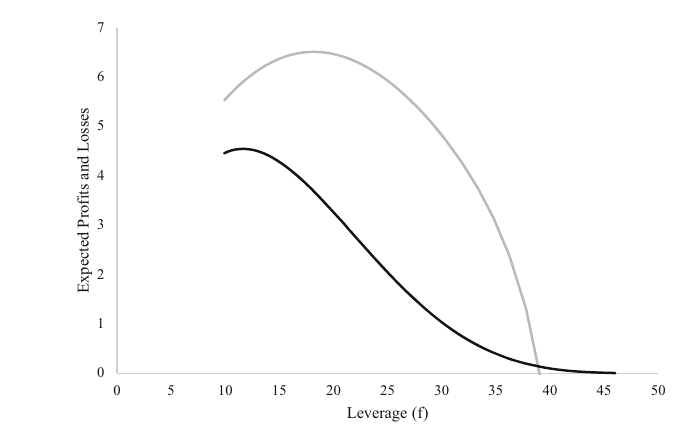
\includegraphics[width=0.85\linewidth]{gfx/m6l4_hott_fig1.png}
\par\smallskip{\small \textbf{Hình 1.} Quan hệ giữa đòn bẩy và lợi nhuận kỳ vọng E(Y) của ngân hàng, cũng như tổn thất kỳ vọng EL của người gửi tiền. P(\ensuremath{\pi}) = 1 \ensuremath{-} \ensuremath{\pi}, I = 50, C = 1 và k(\ensuremath{\pi}) = 0,01/\ensuremath{\pi}. (Nguồn: Hott (2022), Hình 1)}
\end{figure}


Với hai tham số còn lại là C = 1 và I = 50, lợi nhuận đạt cực đại tại \ensuremath{\pi} = 0,21. Hàm chi phí làm cho xác suất vỡ nợ thấp trở nên kém hấp dẫn. Khi chi phí cao hơn, k(\ensuremath{\pi}) = 0,05/\ensuremath{\pi}, xác suất vỡ nợ tối ưu tăng lên 0,23. Đối với các tham số C và I, độ lớn tương đối của chúng quan trọng hơn mức tuyệt đối. Với C = 100

\begin{figure}[H]
\centering
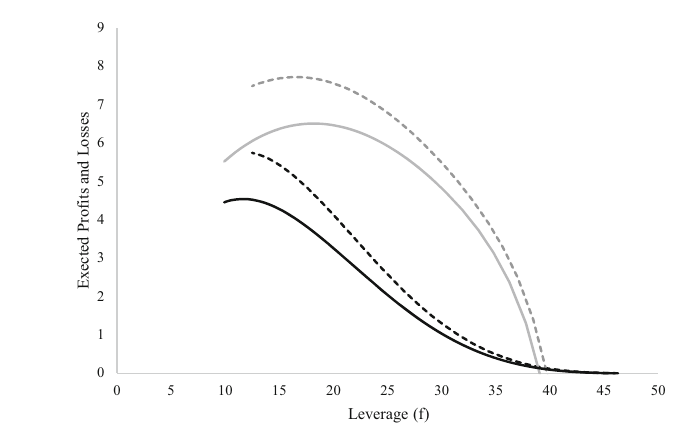
\includegraphics[width=0.85\linewidth]{gfx/m6l4_hott_fig2.png}
\par\smallskip{\small \textbf{Hình 2.} Quan hệ giữa đòn bẩy với tổn thất kỳ vọng (EL và EL\^{}mh) cũng như lợi nhuận kỳ vọng (E(Y) và E(Y\^{}mh)) khi có và không có rủi ro đạo đức. P(\ensuremath{\pi}) = 1 \ensuremath{-} \ensuremath{\pi}, I = 50, C = 1, k(\ensuremath{\pi}) = 0,01/\ensuremath{\pi} và \ensuremath{\beta} = 0,4. (Nguồn: Hott (2022), Hình 2)}
\end{figure}


Khi có bảo lãnh (ngầm định) của chính phủ, tổn thất trực tiếp kỳ vọng của người gửi tiền giảm đi vì chính phủ, với một xác suất nào đó, sẽ chi trả trong trường hợp vỡ nợ. Tuy nhiên, người gửi tiền vẫn chịu tác động gián tiếp vì chính phủ phải tài trợ cho khoản cứu trợ bằng thuế. Do đó, tổn thất kỳ vọng tổng hợp (EL\^{}mh) của người gửi tiền và

\begin{figure}[H]
\centering
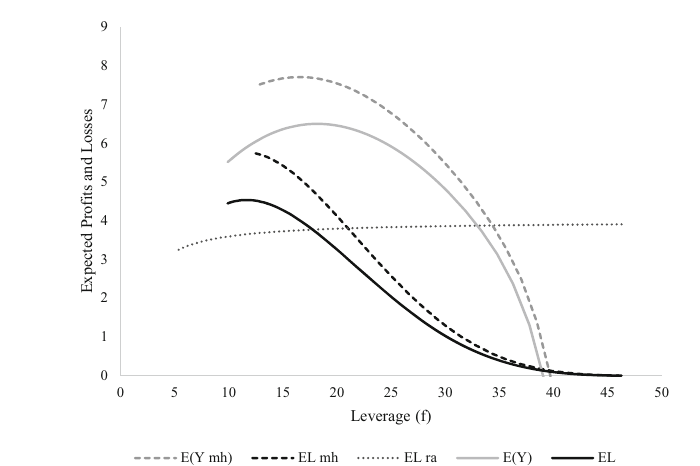
\includegraphics[width=0.85\linewidth]{gfx/m6l4_hott_fig3.png}
\par\smallskip{\small \textbf{Hình 3.} Quan hệ giữa đòn bẩy và các tổn thất kỳ vọng (EL, ELmh và ELra) cũng như lợi nhuận kỳ vọng (E(Y) và E(Y mh)). C = 1, I = 50, \ensuremath{\beta} là 10\%, k(\ensuremath{\pi}) = 0,01/\ensuremath{\pi}, P = 1 \ensuremath{-} \ensuremath{\pi} và \ensuremath{\rho} = 2. (Nguồn: Hott (2022), Hình 3)}
\end{figure}


Các tổn thất tăng đến mức tối đa \ensuremath{\rho}C = 4. Tại đòn bẩy khoảng 18, tổn thất kỳ vọng của ngân hàng hệ thống chịu quy định bằng tổn thất kỳ vọng của chuẩn so sánh (benchmark). Tuy nhiên, đòn bẩy tối đa hóa lợi nhuận khi yêu cầu vốn điều chỉnh theo rủi ro có hiệu lực ràng buộc là khoảng 19 (không hiển thị trong Hình 3).

\chapter{Đọc thêm 3: Phân tích dữ liệu vòng đệm O-ring của Challenger (Wujek)}
\label{ch:M6L4DocThem3}

\section{Thông tin nguồn}

\begin{itemize}
  \item \textbf{Nguồn:} Wujek, J. H. ``Challenger O-Ring Data Analysis.'' Numerical \& Design Problems With Ethical Content, TAMU, 1995.
  \item \textbf{Phần cần đọc:} Toàn bộ
  \item \textbf{Ghi chú:} bản chuyển ngữ tiếng Việt súc tích, bám cấu trúc nguồn (giữ nguyên tiêu đề, công thức, số liệu, bảng, chú thích và danh mục tài liệu tham khảo).
\end{itemize}

\textbf{Tác giả:} Joseph H. Wujek. \textbf{Bộ sưu tập:} Numerical \& Design Problems With Ethical Content. \textbf{Đơn vị:} Zachry Department of Civil Engineering-TAMU Ethics. \textbf{Năm:} 1995. \textbf{DOI:} https://doi.org/10.18130/2pem-7a20

\textbf{Lĩnh vực:} Kỹ thuật hàng không vũ trụ; Khoa học máy tính, toán và vật lý; Kỹ thuật; Khoa học và kỹ thuật vật liệu; Kỹ thuật cơ khí; Thống kê và xác suất.

\textbf{Chủ đề:} Thảm họa, hiểm họa; Quan hệ giữa người sử dụng lao động và người lao động; An toàn phòng thí nghiệm và nơi làm việc; An toàn; Đạo đức nghề nghiệp. Loại: nghiên cứu tình huống.

\subsection{Mô tả}

Tình huống này phân tích dữ liệu vòng đệm O-ring trong thảm họa Challenger và lập luận cho việc hủy bỏ lần phóng. Phù hợp với các môn thống kê ứng dụng, vật liệu và kỹ thuật đại cương (cấp 1-4).

\subsection{Giới thiệu}

Các sự kiện dẫn đến thảm họa Challenger đã được biết rõ. Bài toán này phân tích dữ liệu vòng đệm O-ring và dựa trên kết quả để lập luận về việc hủy phóng.

Dữ liệu ở Bảng 1 được David Hodges sử dụng trong Hội thảo Sinh viên năm nhất tại Đại học California, Berkeley.¹ Đây là dữ liệu của các chuyến bay thành công. Roger Boisjoly cho biết các dữ liệu này chưa có trước thảm họa Challenger.² Hãy dùng dữ liệu Bảng 1 khi cần.³

\begin{enumerate}
\def\labelenumi{\arabic{enumi}.}
\item
  Lập đồ thị hồi quy tuyến tính và ngoại suy kết quả để dự đoán mức hao mòn vật liệu của vòng đệm O-ring tại thời điểm phóng Challenger thảm họa. Giả sử vòng đệm ở nhiệt độ môi trường bệ phóng, 29 °F.

  \begin{enumerate}
  \def\labelenumii{\alph{enumii}.}
    \item
    Tính hệ số tương quan r. So sánh với giá trị tới hạn của r ở mức ý nghĩa 5\% và giải thích ý nghĩa.
  \item
    Bình luận về ý nghĩa của r, \(r^2\) và \(1-r^2\). Điều này có liên quan thế nào khi lập luận không nên phóng?
  \item
    Tính cận khoảng tin cậy 95\% và thể hiện kết quả trên đồ thị tuyến tính.
  \item
    Bình luận về độ phù hợp bằng kiểm định Chi-square (khi bình phương).
  \item
    Bình luận về độ phù hợp bằng kiểm định Kolmogorov-Smirnov.
  \end{enumerate}
\end{enumerate}

\textbf{Bảng 1. Dữ liệu đo sau chuyến bay của Challenger³}

{\small
\begin{longtable}[]{@{}ll@{}}
\toprule\noalign{}
Nhiệt độ O-ring (°F) & Độ sâu xói mòn \ensuremath{\delta} (mil) * \\
\midrule\noalign{}
\endhead
\bottomrule\noalign{}
\endlastfoot
66.0 & 0.0 \\
70.0 & 53.0 \\
69.0 & 0.0 \\
68.0 & 0.0 \\
67.0 & 0.0 \\
72.0 & 0.0 \\
73.0 & 0.0 \\
70.0 & 0.0 \\
57.0 & 40.0 \\
63.0 & 0.0 \\
70.0 & 28.0 \\
78.0 & 0.0 \\
67.0 & 0.0 \\
53.0 & 48.0 \\
67.0 & 0.0 \\
75.0 & 0.0 \\
70.0 & 0.0 \\
81.0 & 0.0 \\
76.0 & 0.0 \\
79.0 & 0.0 \\
75.0 & 0.0 \\
76.0 & 0.0 \\
\end{longtable}
}

* 1 mil bằng \(10^{-3}\) inch.

\begin{enumerate}
\def\labelenumi{\arabic{enumi}.}
\setcounter{enumi}{1}
\item
  Thử khớp các đa thức bậc n = 2, 3, ... với dữ liệu và áp dụng các thước đo ở bài 1(c), (d) và (e) cho kết quả.
\item
  Thử biến đổi tập dữ liệu bằng hàm logarit hoặc hàm lũy thừa rồi khớp hàm tuyến tính với các biến đã biến đổi. Áp dụng các thước đo ở bài 1(c), (d) và (e) cho kết quả và so sánh.
\item
  Với các kết quả trên, dữ liệu sẽ hữu ích đến mức nào khi lập luận cho quyết định "không phóng"? Nhận xét về các hệ quả đạo đức.
\end{enumerate}

\subsection{LỜI GIẢI}

Giả định sinh viên đã được học về các khía cạnh kỹ thuật của thảm họa.

Mục đích của các bài tập là giúp sinh viên nhạy bén với các vấn đề sau:

\begin{itemize}
\item
  Thế giới mang tính xác suất, không tất định, và không có gì là "chắc chắn".
\item
  Dù dữ liệu có thể chưa đủ kết luận, khi tính mạng và tài sản bị đe dọa thì "không biết" phải được coi là "chúng ta đang có vấn đề".
\item
  Hồi quy tuyến tính chỉ là một cách khớp hàm với dữ liệu và diễn giải kết quả về mặt thống kê.
\end{itemize}

\begin{enumerate}
\def\labelenumi{\arabic{enumi}.}
\item
  (Đồ thị được cho bên dưới, phù hợp để làm slide chiếu.) (Phương trình ghi ba chữ số có nghĩa để đối chiếu kết quả.) Tại 29 °F, mức hao hụt vật liệu (độ tin cậy 95 \%) nằm trong khoảng 25 đến 105 mil. Biến thiên cực lớn này cho thấy (xem thêm bên dưới) rủi ro hỏng gioăng rất cao. Dù ngoại suy luôn đáng ngờ, chính việc "không biết" một cách có ý nghĩa thống kê gioăng sẽ hoạt động ra sao ở 29 °F lẽ ra đã là lý do đủ để hủy phóng.

  \begin{enumerate}
  \def\labelenumii{\alph{enumii}.}
  \item
    Từ Hình 1, r = \ensuremath{-}0,56. Tra bảng giá trị tới hạn của hệ số tương quan, ở mức tin cậy 95 \% (mức ý nghĩa 5 \%), với 20 bậc tự do {[}22 cặp dữ liệu trừ hai tham số của phương trình tuyến tính{]}, tìm được \(r_c = 0{,}423\). Điều này có nghĩa là với xác suất 5 \%, dữ liệu có hệ số tương quan lớn đến 0,423 vẫn có thể là không tương quan. Hay nói cách khác, \(r_c\) là giá trị lớn nhất mà \(r\) có thể đạt được chỉ do ngẫu nhiên (trong 95 \% số lần) khi không tồn tại tương quan.
  \item
    Hệ số tương quan r được định nghĩa là: \(r = S_{XY}/(S_X S_Y)\). Tử số là hiệp phương sai mẫu, mẫu số là tích của các độ lệch chuẩn mẫu của hai biến X, Y. Do đó giá trị r là thước đo mức độ liên hệ giữa hai biến. Ta có \(0 \le |r| \le 1\), với \(r = \pm 1\) là tương quan hoàn hảo và \(r = 0\) là hoàn toàn không tương quan. Khi đó \(r^2\) là thước đo phần biến thiên do quan hệ nhân quả, còn \(1 - r^2\) là thước đo phần biến thiên do ngẫu nhiên. Xem thêm các nhận xét ngay sau đề bài ở trên.
  \item
    Xem Hình 1. Giải thích ý nghĩa của khoảng tin cậy. Một cách diễn giải: "Nếu thực hiện một số rất lớn phép thử, 95 \% kết quả sẽ nằm trong khoảng giới hạn 95 \% đã chỉ ra."
  \item
    Đối với cả kiểm định Chi-square và kiểm định K-S ở bài (e), giả thuyết kiểm định là: \(H_0\): dữ liệu không tương quan.

    Ta chấp nhận giả thuyết nếu: \(\chi_0^2 > \chi^2_{1-\alpha,\nu}\)

    trong đó \(1 - \alpha = C\) là mức tin cậy (\(\alpha\) là mức ý nghĩa), và \(\nu\) là số bậc tự do. Ở đây, \(\nu = N - 1 - m\), với N là số quan sát của các biến (22 trong trường hợp này) và m là số tham số của phương trình được kiểm định (m = 2 với phương trình tuyến tính).

    Vế trái của bất đẳng thức là thống kê Chi-square quan sát được, tính từ dữ liệu. Vế phải là giá trị của biến Chi-square ứng với xác suất C, tức là giá trị của tích phân hàm mật độ đến biến ngẫu nhiên đó; các giá trị này đã được lập bảng.

    Với bài toán đang xét: \(\chi^2_{0.95,19} = 30{,}1\) và \(\chi_0^2 = 422\).

    Do đó, giả thuyết được chấp nhận: dữ liệu không tương quan tuyến tính.
  \item
    Với kiểm định Kolmogorov-Smirnov, ta dùng cùng giả thuyết: \(H_0\): dữ liệu không tương quan.

    Ta bác bỏ giả thuyết nếu: \(\sup\{|y_f - y_d|\} \ge d_\alpha(\nu)\)

    Chỉ số dưới của y lần lượt là giá trị "khớp" (fitted) và giá trị "dữ liệu" (data). Như vậy, với một cặp dữ liệu \(x_d, y_d\), giá trị của hàm khớp tại \(x_d\) là \(y_f\). Giá trị lớn nhất ("supremum") được so sánh với thống kê K-S ứng với mức ý nghĩa và số bậc tự do như ở bài (d).

    Ta có \(\sup\{|y_f - y_d|\} = 45\) và \(d_{0.05}(19) = 0{,}301\), nên không thể bác bỏ giả thuyết rằng dữ liệu không tương quan tuyến tính.
  \end{enumerate}
\item
  Bài toán 2 dành cho các bài tập khớp đường cong. Do tính chất mở của bài, không cung cấp lời giải. Một cạm bẫy khi dùng phép biến đổi logarit là cố tính logarit của số không!
\item
  Bài toán 3 dành cho các bài tập khớp đường cong. Do tính chất mở của bài, không cung cấp lời giải. Một cạm bẫy khi dùng phép biến đổi logarit là cố tính logarit của số không!
\item
  Dữ liệu thất thường lẽ ra đã đủ để báo hiệu "chúng ta đang có vấn đề" vì rủi ro đối với tính mạng con người. Các phi hành gia không được thông báo về lịch sử các khiếm khuyết của vòng đệm O-ring, nên không thể có sự đồng thuận có hiểu biết.
\end{enumerate}

\subsection{Chú thích}

\begin{enumerate}
\def\labelenumi{\arabic{enumi}.}
\item
  Lighthall, F. "Launching the Space Shuttle Challenger: Disciplinary Deficiencies in the Analysis of Engineering Data," IEEE Transactions on Engineering Management, Vol. 38, No. 1, February 1991. pp. 63-74.
\item
  Boisjoly, R. Pers. comm. November 1993.
\item
  Lighthall, p. 70, Table I.
\item
  Found in many texts and handbooks. See for example, Fisher, R., and Yates, F., Statistical Tables for Biological. Agricultural, and Medical Research. Oliver \& Boyd, Ltd., Edinburgh, 1957.
\item
  Owen, D. Handbook of Statistical Tables. Addison-Wesley, Reading, MA, 1962. p. 51.
\item
  Owen, p. 64.
\end{enumerate}

Hình 1. Biểu đồ hồi quy tuyến tính trên dữ liệu vòng đệm O-ring (theo Lighthall)

\subsection{Ghi chú}

Tác giả: Dr. Joseph H. Wujek, P.E., College of Engineering, University of California, Berkeley.

Các bài toán này ban đầu được xây dựng trong khuôn khổ một dự án do NSF tài trợ nhằm tạo ra các bài toán số có chứa vấn đề đạo đức, dùng cho bài tập của các môn kỹ thuật và môn học khác. Các bài toán trình bày ở đây đã được chỉnh sửa đôi chút cho rõ ràng.

\subsection{Trích dẫn}

Joseph H. Wujek. 1995. Challenger O-Ring Data Analysis. Online Ethics Center. DOI:https://doi.org/10.18130/2pem-7a20.

\end{document}
